\documentclass[a4paper]{book}
\usepackage{a4wide}
\usepackage{makeidx}
\usepackage{fancyhdr}
\usepackage{graphicx}
\usepackage{multicol}
\usepackage{float}
\usepackage{textcomp}
\usepackage{alltt}
\usepackage{doxygen}
\makeindex
\setcounter{tocdepth}{1}
\renewcommand{\footrulewidth}{0.4pt}
\begin{document}
\begin{titlepage}
\vspace*{7cm}
\begin{center}
{\Large meshmorph Reference Manual\\[1ex]\large 33 }\\
\vspace*{1cm}
{\large Generated by Doxygen 1.5.1}\\
\vspace*{0.5cm}
{\small Fri Feb 13 13:58:10 2009}\\
\end{center}
\end{titlepage}
\clearemptydoublepage
\pagenumbering{roman}
\tableofcontents
\clearemptydoublepage
\pagenumbering{arabic}
\chapter{meshmorph Namespace Index}
\section{meshmorph Namespace List}
Here is a list of all namespaces with brief descriptions:\begin{CompactList}
\item\contentsline{section}{{\bf hxa7241} }{\pageref{namespacehxa7241}}{}
\item\contentsline{section}{{\bf hxa7241\_\-general} }{\pageref{namespacehxa7241__general}}{}
\item\contentsline{section}{{\bf hxa7241\_\-graphics} }{\pageref{namespacehxa7241__graphics}}{}
\item\contentsline{section}{{\bf Wm4} }{\pageref{namespaceWm4}}{}
\end{CompactList}

\chapter{meshmorph Hierarchical Index}
\section{meshmorph Class Hierarchy}
This inheritance list is sorted roughly, but not completely, alphabetically:\begin{CompactList}
\item \contentsline{section}{hxa7241\_\-general::Array$<$ TYPE $>$}{\pageref{classhxa7241__general_1_1Array}}{}
\item \contentsline{section}{Complex}{\pageref{structComplex}}{}
\item \contentsline{section}{Container}{\pageref{classContainer}}{}
\item \contentsline{section}{Controls}{\pageref{classControls}}{}
\item \contentsline{section}{e\_\-hash}{\pageref{structe__hash}}{}
\item \contentsline{section}{Edge}{\pageref{classEdge}}{}
\item \contentsline{section}{Energy}{\pageref{classEnergy}}{}
\item \contentsline{section}{f\_\-hash}{\pageref{structf__hash}}{}
\item \contentsline{section}{Face}{\pageref{classFace}}{}
\item \contentsline{section}{face\_\-grp}{\pageref{structface__grp}}{}
\item \contentsline{section}{Gain\_\-Schedule}{\pageref{classGain__Schedule}}{}
\item \contentsline{section}{Grid}{\pageref{structGrid}}{}
\item \contentsline{section}{Intersecting\_\-Faces}{\pageref{classIntersecting__Faces}}{}
\item \contentsline{section}{Wm4::Intr\-Segment3Triangle3$<$ Real $>$}{\pageref{classWm4_1_1IntrSegment3Triangle3}}{}
\item \contentsline{section}{Wm4::Intr\-Triangle3Cone3$<$ Real $>$}{\pageref{classWm4_1_1IntrTriangle3Cone3}}{}
\item \contentsline{section}{Log}{\pageref{classLog}}{}
\item \contentsline{section}{Wm4::Math$<$ Real $>$}{\pageref{classWm4_1_1Math}}{}
\item \contentsline{section}{Wm4::Matrix3$<$ Real $>$}{\pageref{classWm4_1_1Matrix3}}{}
\item \contentsline{section}{Minmax}{\pageref{structMinmax}}{}
\item \contentsline{section}{my\_\-ltv}{\pageref{structmy__ltv}}{}
\item \contentsline{section}{Nice}{\pageref{classNice}}{}
\item \contentsline{section}{Object}{\pageref{classObject}}{}
\item \contentsline{section}{hxa7241\_\-graphics::Octree$<$ TYPE $>$}{\pageref{classhxa7241__graphics_1_1Octree}}{}
\item \contentsline{section}{hxa7241\_\-graphics::Octree\-Agent\-V}{\pageref{classhxa7241__graphics_1_1OctreeAgentV}}{}
\begin{CompactList}
\item \contentsline{section}{hxa7241\_\-graphics::Octree\-Agent$<$ TYPE $>$}{\pageref{classhxa7241__graphics_1_1OctreeAgent}}{}
\item \contentsline{section}{hxa7241\_\-graphics::Octree\-Agent$<$ Face $>$}{\pageref{classhxa7241__graphics_1_1OctreeAgent}}{}
\begin{CompactList}
\item \contentsline{section}{Octree\_\-Agent\_\-Face}{\pageref{classOctree__Agent__Face}}{}
\end{CompactList}
\end{CompactList}
\item \contentsline{section}{hxa7241\_\-graphics::Octree\-Bound}{\pageref{classhxa7241__graphics_1_1OctreeBound}}{}
\item \contentsline{section}{hxa7241\_\-graphics::Octree\-Cell}{\pageref{classhxa7241__graphics_1_1OctreeCell}}{}
\begin{CompactList}
\item \contentsline{section}{hxa7241\_\-graphics::Octree\-Branch}{\pageref{classhxa7241__graphics_1_1OctreeBranch}}{}
\item \contentsline{section}{hxa7241\_\-graphics::Octree\-Leaf}{\pageref{classhxa7241__graphics_1_1OctreeLeaf}}{}
\end{CompactList}
\item \contentsline{section}{hxa7241\_\-graphics::Octree\-Data}{\pageref{classhxa7241__graphics_1_1OctreeData}}{}
\item \contentsline{section}{hxa7241\_\-graphics::Octree\-Dimensions}{\pageref{classhxa7241__graphics_1_1OctreeDimensions}}{}
\item \contentsline{section}{hxa7241\_\-graphics::Octree\-Root}{\pageref{classhxa7241__graphics_1_1OctreeRoot}}{}
\item \contentsline{section}{hxa7241\_\-graphics::Octree\-Visitor\-V}{\pageref{classhxa7241__graphics_1_1OctreeVisitorV}}{}
\begin{CompactList}
\item \contentsline{section}{hxa7241\_\-graphics::Octree\-Visitor$<$ TYPE $>$}{\pageref{classhxa7241__graphics_1_1OctreeVisitor}}{}
\begin{CompactList}
\item \contentsline{section}{Octree\_\-Visitor\_\-Check\_\-Face}{\pageref{classOctree__Visitor__Check__Face}}{}
\item \contentsline{section}{Octree\_\-Visitor\_\-Face}{\pageref{classOctree__Visitor__Face}}{}
\item \contentsline{section}{Octree\_\-Visitor\_\-Measure}{\pageref{classOctree__Visitor__Measure}}{}
\item \contentsline{section}{Octree\_\-Visitor\_\-Update}{\pageref{classOctree__Visitor__Update}}{}
\end{CompactList}
\item \contentsline{section}{hxa7241\_\-graphics::Octree\-Visitor$<$ Face $>$}{\pageref{classhxa7241__graphics_1_1OctreeVisitor}}{}
\end{CompactList}
\item \contentsline{section}{Wm4::Quaternion$<$ Real $>$}{\pageref{classWm4_1_1Quaternion}}{}
\item \contentsline{section}{Wm4::Quaternion$<$ Real $>$::Constraints}{\pageref{classWm4_1_1Quaternion_1_1Constraints}}{}
\item \contentsline{section}{Refractory}{\pageref{classRefractory}}{}
\item \contentsline{section}{result}{\pageref{structresult}}{}
\item \contentsline{section}{Search\_\-Stats}{\pageref{structSearch__Stats}}{}
\item \contentsline{section}{State}{\pageref{classState}}{}
\item \contentsline{section}{Wm4::System}{\pageref{classWm4_1_1System}}{}
\item \contentsline{section}{Wm4::THash\-Set$<$ TKEY $>$}{\pageref{classWm4_1_1THashSet}}{}
\item \contentsline{section}{Wm4::THash\-Table$<$ TKEY, TVALUE $>$}{\pageref{classWm4_1_1THashTable}}{}
\item \contentsline{section}{Wm4::TMin\-Heap$<$ Generator, Real $>$}{\pageref{classWm4_1_1TMinHeap}}{}
\item \contentsline{section}{Wm4::TMin\-Heap\-Record$<$ Generator, Real $>$}{\pageref{classWm4_1_1TMinHeapRecord}}{}
\item \contentsline{section}{Wm4::TSmall\-Unordered\-Set$<$ T $>$}{\pageref{classWm4_1_1TSmallUnorderedSet}}{}
\item \contentsline{section}{Wm4::TString\-Hash\-Table$<$ TVALUE $>$}{\pageref{classWm4_1_1TStringHashTable}}{}
\item \contentsline{section}{Wm4::TTuple$<$ DIMENSION, TYPE $>$}{\pageref{classWm4_1_1TTuple}}{}
\item \contentsline{section}{v\_\-hash}{\pageref{structv__hash}}{}
\item \contentsline{section}{vector3}{\pageref{structvector3}}{}
\item \contentsline{section}{Wm4::Vector3$<$ Real $>$}{\pageref{classWm4_1_1Vector3}}{}
\item \contentsline{section}{hxa7241\_\-graphics::Vector3r}{\pageref{classhxa7241__graphics_1_1Vector3r}}{}
\item \contentsline{section}{Vertex}{\pageref{classVertex}}{}
\item \contentsline{section}{Vertex\_\-Schedule}{\pageref{classVertex__Schedule}}{}
\item \contentsline{section}{Virtual\_\-Disp}{\pageref{classVirtual__Disp}}{}
\end{CompactList}

\chapter{meshmorph Class Index}
\section{meshmorph Class List}
Here are the classes, structs, unions and interfaces with brief descriptions:\begin{CompactList}
\item\contentsline{section}{{\bf hxa7241\_\-general::Array$<$ TYPE $>$} }{\pageref{classhxa7241__general_1_1Array}}{}
\item\contentsline{section}{{\bf Complex} }{\pageref{structComplex}}{}
\item\contentsline{section}{{\bf Container} }{\pageref{classContainer}}{}
\item\contentsline{section}{{\bf Controls} }{\pageref{classControls}}{}
\item\contentsline{section}{{\bf e\_\-hash} }{\pageref{structe__hash}}{}
\item\contentsline{section}{{\bf Edge} }{\pageref{classEdge}}{}
\item\contentsline{section}{{\bf Energy} }{\pageref{classEnergy}}{}
\item\contentsline{section}{{\bf f\_\-hash} }{\pageref{structf__hash}}{}
\item\contentsline{section}{{\bf Face} }{\pageref{classFace}}{}
\item\contentsline{section}{{\bf face\_\-grp} }{\pageref{structface__grp}}{}
\item\contentsline{section}{{\bf Gain\_\-Schedule} }{\pageref{classGain__Schedule}}{}
\item\contentsline{section}{{\bf Grid} }{\pageref{structGrid}}{}
\item\contentsline{section}{{\bf Intersecting\_\-Faces} }{\pageref{classIntersecting__Faces}}{}
\item\contentsline{section}{{\bf Wm4::Intr\-Segment3Triangle3$<$ Real $>$} }{\pageref{classWm4_1_1IntrSegment3Triangle3}}{}
\item\contentsline{section}{{\bf Wm4::Intr\-Triangle3Cone3$<$ Real $>$} }{\pageref{classWm4_1_1IntrTriangle3Cone3}}{}
\item\contentsline{section}{{\bf Log} }{\pageref{classLog}}{}
\item\contentsline{section}{{\bf Wm4::Math$<$ Real $>$} }{\pageref{classWm4_1_1Math}}{}
\item\contentsline{section}{{\bf Wm4::Matrix3$<$ Real $>$} }{\pageref{classWm4_1_1Matrix3}}{}
\item\contentsline{section}{{\bf Minmax} }{\pageref{structMinmax}}{}
\item\contentsline{section}{{\bf my\_\-ltv} }{\pageref{structmy__ltv}}{}
\item\contentsline{section}{{\bf Nice} }{\pageref{classNice}}{}
\item\contentsline{section}{{\bf Object} }{\pageref{classObject}}{}
\item\contentsline{section}{{\bf hxa7241\_\-graphics::Octree$<$ TYPE $>$} }{\pageref{classhxa7241__graphics_1_1Octree}}{}
\item\contentsline{section}{{\bf Octree\_\-Agent\_\-Face} }{\pageref{classOctree__Agent__Face}}{}
\item\contentsline{section}{{\bf Octree\_\-Visitor\_\-Check\_\-Face} }{\pageref{classOctree__Visitor__Check__Face}}{}
\item\contentsline{section}{{\bf Octree\_\-Visitor\_\-Face} }{\pageref{classOctree__Visitor__Face}}{}
\item\contentsline{section}{{\bf Octree\_\-Visitor\_\-Measure} }{\pageref{classOctree__Visitor__Measure}}{}
\item\contentsline{section}{{\bf Octree\_\-Visitor\_\-Update} }{\pageref{classOctree__Visitor__Update}}{}
\item\contentsline{section}{{\bf hxa7241\_\-graphics::Octree\-Agent$<$ TYPE $>$} }{\pageref{classhxa7241__graphics_1_1OctreeAgent}}{}
\item\contentsline{section}{{\bf hxa7241\_\-graphics::Octree\-Agent\-V} }{\pageref{classhxa7241__graphics_1_1OctreeAgentV}}{}
\item\contentsline{section}{{\bf hxa7241\_\-graphics::Octree\-Bound} }{\pageref{classhxa7241__graphics_1_1OctreeBound}}{}
\item\contentsline{section}{{\bf hxa7241\_\-graphics::Octree\-Branch} }{\pageref{classhxa7241__graphics_1_1OctreeBranch}}{}
\item\contentsline{section}{{\bf hxa7241\_\-graphics::Octree\-Cell} }{\pageref{classhxa7241__graphics_1_1OctreeCell}}{}
\item\contentsline{section}{{\bf hxa7241\_\-graphics::Octree\-Data} }{\pageref{classhxa7241__graphics_1_1OctreeData}}{}
\item\contentsline{section}{{\bf hxa7241\_\-graphics::Octree\-Dimensions} }{\pageref{classhxa7241__graphics_1_1OctreeDimensions}}{}
\item\contentsline{section}{{\bf hxa7241\_\-graphics::Octree\-Leaf} }{\pageref{classhxa7241__graphics_1_1OctreeLeaf}}{}
\item\contentsline{section}{{\bf hxa7241\_\-graphics::Octree\-Root} }{\pageref{classhxa7241__graphics_1_1OctreeRoot}}{}
\item\contentsline{section}{{\bf hxa7241\_\-graphics::Octree\-Visitor$<$ TYPE $>$} }{\pageref{classhxa7241__graphics_1_1OctreeVisitor}}{}
\item\contentsline{section}{{\bf hxa7241\_\-graphics::Octree\-Visitor\-V} }{\pageref{classhxa7241__graphics_1_1OctreeVisitorV}}{}
\item\contentsline{section}{{\bf Wm4::Quaternion$<$ Real $>$} }{\pageref{classWm4_1_1Quaternion}}{}
\item\contentsline{section}{{\bf Wm4::Quaternion$<$ Real $>$::Constraints} }{\pageref{classWm4_1_1Quaternion_1_1Constraints}}{}
\item\contentsline{section}{{\bf Refractory} }{\pageref{classRefractory}}{}
\item\contentsline{section}{{\bf result} }{\pageref{structresult}}{}
\item\contentsline{section}{{\bf Search\_\-Stats} }{\pageref{structSearch__Stats}}{}
\item\contentsline{section}{{\bf State} }{\pageref{classState}}{}
\item\contentsline{section}{{\bf Wm4::System} }{\pageref{classWm4_1_1System}}{}
\item\contentsline{section}{{\bf Wm4::THash\-Set$<$ TKEY $>$} }{\pageref{classWm4_1_1THashSet}}{}
\item\contentsline{section}{{\bf Wm4::THash\-Table$<$ TKEY, TVALUE $>$} }{\pageref{classWm4_1_1THashTable}}{}
\item\contentsline{section}{{\bf Wm4::TMin\-Heap$<$ Generator, Real $>$} }{\pageref{classWm4_1_1TMinHeap}}{}
\item\contentsline{section}{{\bf Wm4::TMin\-Heap\-Record$<$ Generator, Real $>$} }{\pageref{classWm4_1_1TMinHeapRecord}}{}
\item\contentsline{section}{{\bf Wm4::TSmall\-Unordered\-Set$<$ T $>$} }{\pageref{classWm4_1_1TSmallUnorderedSet}}{}
\item\contentsline{section}{{\bf Wm4::TString\-Hash\-Table$<$ TVALUE $>$} }{\pageref{classWm4_1_1TStringHashTable}}{}
\item\contentsline{section}{{\bf Wm4::TTuple$<$ DIMENSION, TYPE $>$} }{\pageref{classWm4_1_1TTuple}}{}
\item\contentsline{section}{{\bf v\_\-hash} }{\pageref{structv__hash}}{}
\item\contentsline{section}{{\bf vector3} }{\pageref{structvector3}}{}
\item\contentsline{section}{{\bf Wm4::Vector3$<$ Real $>$} }{\pageref{classWm4_1_1Vector3}}{}
\item\contentsline{section}{{\bf hxa7241\_\-graphics::Vector3r} }{\pageref{classhxa7241__graphics_1_1Vector3r}}{}
\item\contentsline{section}{{\bf Vertex} }{\pageref{classVertex}}{}
\item\contentsline{section}{{\bf Vertex\_\-Schedule} }{\pageref{classVertex__Schedule}}{}
\item\contentsline{section}{{\bf Virtual\_\-Disp} }{\pageref{classVirtual__Disp}}{}
\end{CompactList}

\chapter{meshmorph File Index}
\section{File List}
Here is a list of all files with brief descriptions:\begin{CompactList}
\item\contentsline{section}{\hyperlink{container_8cc}{container.cc} }{\pageref{container_8cc}}{}
\item\contentsline{section}{\hyperlink{container_8h}{container.h} }{\pageref{container_8h}}{}
\item\contentsline{section}{\hyperlink{contour_8cc}{contour.cc} }{\pageref{contour_8cc}}{}
\item\contentsline{section}{\hyperlink{contour_8h}{contour.h} }{\pageref{contour_8h}}{}
\item\contentsline{section}{\hyperlink{control__points_8cc}{control\_\-points.cc} }{\pageref{control__points_8cc}}{}
\item\contentsline{section}{\hyperlink{control__points_8h}{control\_\-points.h} }{\pageref{control__points_8h}}{}
\item\contentsline{section}{\hyperlink{controls_8cc}{controls.cc} }{\pageref{controls_8cc}}{}
\item\contentsline{section}{\hyperlink{controls_8h}{controls.h} }{\pageref{controls_8h}}{}
\item\contentsline{section}{\hyperlink{histogram_8cc}{histogram.cc} }{\pageref{histogram_8cc}}{}
\item\contentsline{section}{\hyperlink{histogram_8h}{histogram.h} }{\pageref{histogram_8h}}{}
\item\contentsline{section}{\hyperlink{object_8cc}{object.cc} }{\pageref{object_8cc}}{}
\item\contentsline{section}{\hyperlink{object_8h}{object.h} }{\pageref{object_8h}}{}
\item\contentsline{section}{\hyperlink{parameter_8cc}{parameter.cc} }{\pageref{parameter_8cc}}{}
\item\contentsline{section}{\hyperlink{parameter_8h}{parameter.h} }{\pageref{parameter_8h}}{}
\item\contentsline{section}{\hyperlink{point_8cc}{point.cc} }{\pageref{point_8cc}}{}
\item\contentsline{section}{\hyperlink{point_8h}{point.h} }{\pageref{point_8h}}{}
\item\contentsline{section}{\hyperlink{proximity__energy_8m}{proximity\_\-energy.m} }{\pageref{proximity__energy_8m}}{}
\item\contentsline{section}{\hyperlink{reconstruct2contourtiler_8cc}{reconstruct2contourtiler.cc} }{\pageref{reconstruct2contourtiler_8cc}}{}
\item\contentsline{section}{\hyperlink{reconstruct2contourtiler_8h}{reconstruct2contourtiler.h} }{\pageref{reconstruct2contourtiler_8h}}{}
\item\contentsline{section}{\hyperlink{sim__anneal_8cc}{sim\_\-anneal.cc} }{\pageref{sim__anneal_8cc}}{}
\item\contentsline{section}{\hyperlink{sim__anneal_8h}{sim\_\-anneal.h} }{\pageref{sim__anneal_8h}}{}
\end{CompactList}

\chapter{meshmorph Namespace Documentation}
\section{hxa7241 Namespace Reference}
\label{namespacehxa7241}\index{hxa7241@{hxa7241}}


\subsection*{Typedefs}
\begin{CompactItemize}
\item 
typedef signed char {\bf byte}
\begin{CompactList}\small\item\em types ---------------------------------------------------------------------- \item\end{CompactList}\item 
typedef unsigned char {\bf ubyte}
\item 
typedef signed short {\bf word}
\item 
typedef unsigned short {\bf uword}
\item 
typedef signed int {\bf dword}
\item 
typedef unsigned int {\bf udword}
\item 
typedef double {\bf real}
\end{CompactItemize}
\subsection*{Variables}
\begin{CompactItemize}
\item 
const {\bf byte} {\bf BYTE\_\-MIN} = SCHAR\_\-MIN
\begin{CompactList}\small\item\em constants ------------------------------------------------------------------ \item\end{CompactList}\item 
const {\bf byte} {\bf BYTE\_\-MAX} = SCHAR\_\-MAX
\item 
const int {\bf BYTE\_\-BITS} = 8
\item 
const {\bf ubyte} {\bf UBYTE\_\-MIN} = 0
\item 
const {\bf ubyte} {\bf UBYTE\_\-MAX} = UCHAR\_\-MAX
\item 
const int {\bf UBYTE\_\-BITS} = 8
\item 
const {\bf word} {\bf WORD\_\-MIN} = SHRT\_\-MIN
\item 
const {\bf word} {\bf WORD\_\-MAX} = SHRT\_\-MAX
\item 
const int {\bf WORD\_\-BITS} = 16
\item 
const {\bf uword} {\bf UWORD\_\-MIN} = 0
\item 
const {\bf uword} {\bf UWORD\_\-MAX} = USHRT\_\-MAX
\item 
const int {\bf UWORD\_\-BITS} = 16
\item 
const {\bf dword} {\bf DWORD\_\-MIN} = INT\_\-MIN
\item 
const {\bf dword} {\bf DWORD\_\-MAX} = INT\_\-MAX
\item 
const int {\bf DWORD\_\-BITS} = 32
\item 
const {\bf udword} {\bf UDWORD\_\-MIN} = 0
\item 
const {\bf udword} {\bf UDWORD\_\-MAX} = UINT\_\-MAX
\item 
const int {\bf UDWORD\_\-BITS} = 32
\item 
const float {\bf FLOAT\_\-MIN\_\-POS} = static\_\-cast$<$float$>$(FLT\_\-MIN)
\item 
const float {\bf FLOAT\_\-MIN\_\-NEG} = static\_\-cast$<$float$>$(-FLT\_\-MAX)
\item 
const float {\bf FLOAT\_\-MAX} = static\_\-cast$<$float$>$(FLT\_\-MAX)
\item 
const float {\bf FLOAT\_\-EPSILON} = static\_\-cast$<$float$>$(FLT\_\-EPSILON)
\item 
const float {\bf FLOAT\_\-ALMOST\_\-ONE} = static\_\-cast$<$float$>$(1.0f - FLT\_\-EPSILON)
\item 
const float {\bf FLOAT\_\-SMALL} = static\_\-cast$<$float$>$(1.0e-12f)
\item 
const float {\bf FLOAT\_\-LARGE} = static\_\-cast$<$float$>$(1.0e+12f)
\item 
const double {\bf DOUBLE\_\-MIN\_\-POS} = static\_\-cast$<$double$>$(DBL\_\-MIN)
\item 
const double {\bf DOUBLE\_\-MIN\_\-NEG} = static\_\-cast$<$double$>$(-DBL\_\-MAX)
\item 
const double {\bf DOUBLE\_\-MAX} = static\_\-cast$<$double$>$(DBL\_\-MAX)
\item 
const double {\bf DOUBLE\_\-EPSILON} = static\_\-cast$<$double$>$(DBL\_\-EPSILON)
\item 
const double {\bf DOUBLE\_\-ALMOST\_\-ONE} = static\_\-cast$<$double$>$(1.0 - DBL\_\-EPSILON)
\item 
const double {\bf DOUBLE\_\-SMALL} = static\_\-cast$<$double$>$(1.0e-96)
\item 
const double {\bf DOUBLE\_\-LARGE} = static\_\-cast$<$double$>$(1.0e+96)
\item 
const double {\bf REAL\_\-MIN\_\-POS} = {\bf DOUBLE\_\-MIN\_\-POS}
\item 
const double {\bf REAL\_\-MIN\_\-NEG} = {\bf DOUBLE\_\-MIN\_\-NEG}
\item 
const double {\bf REAL\_\-MAX} = {\bf DOUBLE\_\-MAX}
\item 
const double {\bf REAL\_\-EPSILON} = {\bf DOUBLE\_\-EPSILON}
\item 
const double {\bf REAL\_\-ALMOST\_\-ONE} = {\bf DOUBLE\_\-ALMOST\_\-ONE}
\item 
const double {\bf REAL\_\-SMALL} = {\bf DOUBLE\_\-SMALL}
\item 
const double {\bf REAL\_\-LARGE} = {\bf DOUBLE\_\-LARGE}
\end{CompactItemize}


\subsection{Typedef Documentation}
\index{hxa7241@{hxa7241}!byte@{byte}}
\index{byte@{byte}!hxa7241@{hxa7241}}
\subsubsection{\setlength{\rightskip}{0pt plus 5cm}typedef signed char {\bf hxa7241::byte}}\label{namespacehxa7241_f9f106c86bb3c811a94166a414427ab4}


types ---------------------------------------------------------------------- 

\index{hxa7241@{hxa7241}!dword@{dword}}
\index{dword@{dword}!hxa7241@{hxa7241}}
\subsubsection{\setlength{\rightskip}{0pt plus 5cm}typedef signed int {\bf hxa7241::dword}}\label{namespacehxa7241_bcd38545952886f4718dd5f32b2c5a29}


\index{hxa7241@{hxa7241}!real@{real}}
\index{real@{real}!hxa7241@{hxa7241}}
\subsubsection{\setlength{\rightskip}{0pt plus 5cm}typedef double {\bf hxa7241::real}}\label{namespacehxa7241_59e97cee28216d10a7456904131c03e2}


\index{hxa7241@{hxa7241}!ubyte@{ubyte}}
\index{ubyte@{ubyte}!hxa7241@{hxa7241}}
\subsubsection{\setlength{\rightskip}{0pt plus 5cm}typedef unsigned char {\bf hxa7241::ubyte}}\label{namespacehxa7241_fab3e7e85b1e21a7f958fd1335a29267}


\index{hxa7241@{hxa7241}!udword@{udword}}
\index{udword@{udword}!hxa7241@{hxa7241}}
\subsubsection{\setlength{\rightskip}{0pt plus 5cm}typedef unsigned int {\bf hxa7241::udword}}\label{namespacehxa7241_2eca61fc527a2cb781fb2b30ab6a7196}


\index{hxa7241@{hxa7241}!uword@{uword}}
\index{uword@{uword}!hxa7241@{hxa7241}}
\subsubsection{\setlength{\rightskip}{0pt plus 5cm}typedef unsigned short {\bf hxa7241::uword}}\label{namespacehxa7241_4cdf1512ec5528bf1f7e620c3b02550e}


\index{hxa7241@{hxa7241}!word@{word}}
\index{word@{word}!hxa7241@{hxa7241}}
\subsubsection{\setlength{\rightskip}{0pt plus 5cm}typedef signed short {\bf hxa7241::word}}\label{namespacehxa7241_af2eb8e13a846666d2f01e67472f2315}




\subsection{Variable Documentation}
\index{hxa7241@{hxa7241}!BYTE_BITS@{BYTE\_\-BITS}}
\index{BYTE_BITS@{BYTE\_\-BITS}!hxa7241@{hxa7241}}
\subsubsection{\setlength{\rightskip}{0pt plus 5cm}const int {\bf hxa7241::BYTE\_\-BITS} = 8}\label{namespacehxa7241_c802cdb38c9d21ee955d63d4ec4fd99c}


\index{hxa7241@{hxa7241}!BYTE_MAX@{BYTE\_\-MAX}}
\index{BYTE_MAX@{BYTE\_\-MAX}!hxa7241@{hxa7241}}
\subsubsection{\setlength{\rightskip}{0pt plus 5cm}const {\bf byte} {\bf hxa7241::BYTE\_\-MAX} = SCHAR\_\-MAX}\label{namespacehxa7241_f59c9ac5ab7a08e8a401541c5f92500d}


\index{hxa7241@{hxa7241}!BYTE_MIN@{BYTE\_\-MIN}}
\index{BYTE_MIN@{BYTE\_\-MIN}!hxa7241@{hxa7241}}
\subsubsection{\setlength{\rightskip}{0pt plus 5cm}const {\bf byte} {\bf hxa7241::BYTE\_\-MIN} = SCHAR\_\-MIN}\label{namespacehxa7241_611bdcb31914ce386ba010c3bae70ca2}


constants ------------------------------------------------------------------ 

\index{hxa7241@{hxa7241}!DOUBLE_ALMOST_ONE@{DOUBLE\_\-ALMOST\_\-ONE}}
\index{DOUBLE_ALMOST_ONE@{DOUBLE\_\-ALMOST\_\-ONE}!hxa7241@{hxa7241}}
\subsubsection{\setlength{\rightskip}{0pt plus 5cm}const double {\bf hxa7241::DOUBLE\_\-ALMOST\_\-ONE} = static\_\-cast$<$double$>$(1.0 - DBL\_\-EPSILON)}\label{namespacehxa7241_dc69c21791f41d1dec6484feba84e78b}


\index{hxa7241@{hxa7241}!DOUBLE_EPSILON@{DOUBLE\_\-EPSILON}}
\index{DOUBLE_EPSILON@{DOUBLE\_\-EPSILON}!hxa7241@{hxa7241}}
\subsubsection{\setlength{\rightskip}{0pt plus 5cm}const double {\bf hxa7241::DOUBLE\_\-EPSILON} = static\_\-cast$<$double$>$(DBL\_\-EPSILON)}\label{namespacehxa7241_4ca720e502303c8ff466000e00779167}


\index{hxa7241@{hxa7241}!DOUBLE_LARGE@{DOUBLE\_\-LARGE}}
\index{DOUBLE_LARGE@{DOUBLE\_\-LARGE}!hxa7241@{hxa7241}}
\subsubsection{\setlength{\rightskip}{0pt plus 5cm}const double {\bf hxa7241::DOUBLE\_\-LARGE} = static\_\-cast$<$double$>$(1.0e+96)}\label{namespacehxa7241_c5793cdbd6528204aa1941c431f054ba}


\index{hxa7241@{hxa7241}!DOUBLE_MAX@{DOUBLE\_\-MAX}}
\index{DOUBLE_MAX@{DOUBLE\_\-MAX}!hxa7241@{hxa7241}}
\subsubsection{\setlength{\rightskip}{0pt plus 5cm}const double {\bf hxa7241::DOUBLE\_\-MAX} = static\_\-cast$<$double$>$(DBL\_\-MAX)}\label{namespacehxa7241_c96d6f5b1b2d6308f9641677c6f070fc}


\index{hxa7241@{hxa7241}!DOUBLE_MIN_NEG@{DOUBLE\_\-MIN\_\-NEG}}
\index{DOUBLE_MIN_NEG@{DOUBLE\_\-MIN\_\-NEG}!hxa7241@{hxa7241}}
\subsubsection{\setlength{\rightskip}{0pt plus 5cm}const double {\bf hxa7241::DOUBLE\_\-MIN\_\-NEG} = static\_\-cast$<$double$>$(-DBL\_\-MAX)}\label{namespacehxa7241_a9629489df8ef535266f11220c0744a8}


\index{hxa7241@{hxa7241}!DOUBLE_MIN_POS@{DOUBLE\_\-MIN\_\-POS}}
\index{DOUBLE_MIN_POS@{DOUBLE\_\-MIN\_\-POS}!hxa7241@{hxa7241}}
\subsubsection{\setlength{\rightskip}{0pt plus 5cm}const double {\bf hxa7241::DOUBLE\_\-MIN\_\-POS} = static\_\-cast$<$double$>$(DBL\_\-MIN)}\label{namespacehxa7241_4346063ac57e1eca8b123fc5d74bda60}


\index{hxa7241@{hxa7241}!DOUBLE_SMALL@{DOUBLE\_\-SMALL}}
\index{DOUBLE_SMALL@{DOUBLE\_\-SMALL}!hxa7241@{hxa7241}}
\subsubsection{\setlength{\rightskip}{0pt plus 5cm}const double {\bf hxa7241::DOUBLE\_\-SMALL} = static\_\-cast$<$double$>$(1.0e-96)}\label{namespacehxa7241_82624246707fba349d1d4128e2165da2}


\index{hxa7241@{hxa7241}!DWORD_BITS@{DWORD\_\-BITS}}
\index{DWORD_BITS@{DWORD\_\-BITS}!hxa7241@{hxa7241}}
\subsubsection{\setlength{\rightskip}{0pt plus 5cm}const int {\bf hxa7241::DWORD\_\-BITS} = 32}\label{namespacehxa7241_98add39fa8e129dce90bd4d5b713654d}


\index{hxa7241@{hxa7241}!DWORD_MAX@{DWORD\_\-MAX}}
\index{DWORD_MAX@{DWORD\_\-MAX}!hxa7241@{hxa7241}}
\subsubsection{\setlength{\rightskip}{0pt plus 5cm}const {\bf dword} {\bf hxa7241::DWORD\_\-MAX} = INT\_\-MAX}\label{namespacehxa7241_695c61218401c8b2037d44df891197de}


\index{hxa7241@{hxa7241}!DWORD_MIN@{DWORD\_\-MIN}}
\index{DWORD_MIN@{DWORD\_\-MIN}!hxa7241@{hxa7241}}
\subsubsection{\setlength{\rightskip}{0pt plus 5cm}const {\bf dword} {\bf hxa7241::DWORD\_\-MIN} = INT\_\-MIN}\label{namespacehxa7241_6812ba25c03cea3ac61c640bb57189a6}


\index{hxa7241@{hxa7241}!FLOAT_ALMOST_ONE@{FLOAT\_\-ALMOST\_\-ONE}}
\index{FLOAT_ALMOST_ONE@{FLOAT\_\-ALMOST\_\-ONE}!hxa7241@{hxa7241}}
\subsubsection{\setlength{\rightskip}{0pt plus 5cm}const float {\bf hxa7241::FLOAT\_\-ALMOST\_\-ONE} = static\_\-cast$<$float$>$(1.0f - FLT\_\-EPSILON)}\label{namespacehxa7241_2b4e780116de88f676fb1cf7baa8547f}


\index{hxa7241@{hxa7241}!FLOAT_EPSILON@{FLOAT\_\-EPSILON}}
\index{FLOAT_EPSILON@{FLOAT\_\-EPSILON}!hxa7241@{hxa7241}}
\subsubsection{\setlength{\rightskip}{0pt plus 5cm}const float {\bf hxa7241::FLOAT\_\-EPSILON} = static\_\-cast$<$float$>$(FLT\_\-EPSILON)}\label{namespacehxa7241_1c1abb83af1eaa2c69272cf6cca3bb0a}


\index{hxa7241@{hxa7241}!FLOAT_LARGE@{FLOAT\_\-LARGE}}
\index{FLOAT_LARGE@{FLOAT\_\-LARGE}!hxa7241@{hxa7241}}
\subsubsection{\setlength{\rightskip}{0pt plus 5cm}const float {\bf hxa7241::FLOAT\_\-LARGE} = static\_\-cast$<$float$>$(1.0e+12f)}\label{namespacehxa7241_3e7fc9606463c22343f046d0befb25f6}


\index{hxa7241@{hxa7241}!FLOAT_MAX@{FLOAT\_\-MAX}}
\index{FLOAT_MAX@{FLOAT\_\-MAX}!hxa7241@{hxa7241}}
\subsubsection{\setlength{\rightskip}{0pt plus 5cm}const float {\bf hxa7241::FLOAT\_\-MAX} = static\_\-cast$<$float$>$(FLT\_\-MAX)}\label{namespacehxa7241_54f62fe96affb3f699b92d88fd7e06b4}


\index{hxa7241@{hxa7241}!FLOAT_MIN_NEG@{FLOAT\_\-MIN\_\-NEG}}
\index{FLOAT_MIN_NEG@{FLOAT\_\-MIN\_\-NEG}!hxa7241@{hxa7241}}
\subsubsection{\setlength{\rightskip}{0pt plus 5cm}const float {\bf hxa7241::FLOAT\_\-MIN\_\-NEG} = static\_\-cast$<$float$>$(-FLT\_\-MAX)}\label{namespacehxa7241_20436bf56f732a7069b399899de886ed}


\index{hxa7241@{hxa7241}!FLOAT_MIN_POS@{FLOAT\_\-MIN\_\-POS}}
\index{FLOAT_MIN_POS@{FLOAT\_\-MIN\_\-POS}!hxa7241@{hxa7241}}
\subsubsection{\setlength{\rightskip}{0pt plus 5cm}const float {\bf hxa7241::FLOAT\_\-MIN\_\-POS} = static\_\-cast$<$float$>$(FLT\_\-MIN)}\label{namespacehxa7241_52f6258541564b64550f0ca3fa3ce3f5}


\index{hxa7241@{hxa7241}!FLOAT_SMALL@{FLOAT\_\-SMALL}}
\index{FLOAT_SMALL@{FLOAT\_\-SMALL}!hxa7241@{hxa7241}}
\subsubsection{\setlength{\rightskip}{0pt plus 5cm}const float {\bf hxa7241::FLOAT\_\-SMALL} = static\_\-cast$<$float$>$(1.0e-12f)}\label{namespacehxa7241_b8f869ddf6dcec3226201c4df448e1d7}


\index{hxa7241@{hxa7241}!REAL_ALMOST_ONE@{REAL\_\-ALMOST\_\-ONE}}
\index{REAL_ALMOST_ONE@{REAL\_\-ALMOST\_\-ONE}!hxa7241@{hxa7241}}
\subsubsection{\setlength{\rightskip}{0pt plus 5cm}const double {\bf hxa7241::REAL\_\-ALMOST\_\-ONE} = {\bf DOUBLE\_\-ALMOST\_\-ONE}}\label{namespacehxa7241_141e6b07cad91128f60b5aa6778b37cb}


\index{hxa7241@{hxa7241}!REAL_EPSILON@{REAL\_\-EPSILON}}
\index{REAL_EPSILON@{REAL\_\-EPSILON}!hxa7241@{hxa7241}}
\subsubsection{\setlength{\rightskip}{0pt plus 5cm}const double {\bf hxa7241::REAL\_\-EPSILON} = {\bf DOUBLE\_\-EPSILON}}\label{namespacehxa7241_e6f0fc0eacc944c6869a65e0328c386e}


\index{hxa7241@{hxa7241}!REAL_LARGE@{REAL\_\-LARGE}}
\index{REAL_LARGE@{REAL\_\-LARGE}!hxa7241@{hxa7241}}
\subsubsection{\setlength{\rightskip}{0pt plus 5cm}const double {\bf hxa7241::REAL\_\-LARGE} = {\bf DOUBLE\_\-LARGE}}\label{namespacehxa7241_2b48c7e1783ee552f43c4f8839c95ced}


\index{hxa7241@{hxa7241}!REAL_MAX@{REAL\_\-MAX}}
\index{REAL_MAX@{REAL\_\-MAX}!hxa7241@{hxa7241}}
\subsubsection{\setlength{\rightskip}{0pt plus 5cm}const double {\bf hxa7241::REAL\_\-MAX} = {\bf DOUBLE\_\-MAX}}\label{namespacehxa7241_380c050c11695752ff7b39f3805a3868}


\index{hxa7241@{hxa7241}!REAL_MIN_NEG@{REAL\_\-MIN\_\-NEG}}
\index{REAL_MIN_NEG@{REAL\_\-MIN\_\-NEG}!hxa7241@{hxa7241}}
\subsubsection{\setlength{\rightskip}{0pt plus 5cm}const double {\bf hxa7241::REAL\_\-MIN\_\-NEG} = {\bf DOUBLE\_\-MIN\_\-NEG}}\label{namespacehxa7241_9adfd9003355ed1cf3a89e4d6971c5e1}


\index{hxa7241@{hxa7241}!REAL_MIN_POS@{REAL\_\-MIN\_\-POS}}
\index{REAL_MIN_POS@{REAL\_\-MIN\_\-POS}!hxa7241@{hxa7241}}
\subsubsection{\setlength{\rightskip}{0pt plus 5cm}const double {\bf hxa7241::REAL\_\-MIN\_\-POS} = {\bf DOUBLE\_\-MIN\_\-POS}}\label{namespacehxa7241_b525ac3ca9aeca68c69a5b672398589b}


\index{hxa7241@{hxa7241}!REAL_SMALL@{REAL\_\-SMALL}}
\index{REAL_SMALL@{REAL\_\-SMALL}!hxa7241@{hxa7241}}
\subsubsection{\setlength{\rightskip}{0pt plus 5cm}const double {\bf hxa7241::REAL\_\-SMALL} = {\bf DOUBLE\_\-SMALL}}\label{namespacehxa7241_3acdce9acb0aa49597564e9a4250cc47}


\index{hxa7241@{hxa7241}!UBYTE_BITS@{UBYTE\_\-BITS}}
\index{UBYTE_BITS@{UBYTE\_\-BITS}!hxa7241@{hxa7241}}
\subsubsection{\setlength{\rightskip}{0pt plus 5cm}const int {\bf hxa7241::UBYTE\_\-BITS} = 8}\label{namespacehxa7241_4ba3d00b9d684194124a3fbff57fcb63}


\index{hxa7241@{hxa7241}!UBYTE_MAX@{UBYTE\_\-MAX}}
\index{UBYTE_MAX@{UBYTE\_\-MAX}!hxa7241@{hxa7241}}
\subsubsection{\setlength{\rightskip}{0pt plus 5cm}const {\bf ubyte} {\bf hxa7241::UBYTE\_\-MAX} = UCHAR\_\-MAX}\label{namespacehxa7241_7c80885229aeca6dd516ec489663fc12}


\index{hxa7241@{hxa7241}!UBYTE_MIN@{UBYTE\_\-MIN}}
\index{UBYTE_MIN@{UBYTE\_\-MIN}!hxa7241@{hxa7241}}
\subsubsection{\setlength{\rightskip}{0pt plus 5cm}const {\bf ubyte} {\bf hxa7241::UBYTE\_\-MIN} = 0}\label{namespacehxa7241_985afaf4f35143a7f95b3e637b1b6cdc}


\index{hxa7241@{hxa7241}!UDWORD_BITS@{UDWORD\_\-BITS}}
\index{UDWORD_BITS@{UDWORD\_\-BITS}!hxa7241@{hxa7241}}
\subsubsection{\setlength{\rightskip}{0pt plus 5cm}const int {\bf hxa7241::UDWORD\_\-BITS} = 32}\label{namespacehxa7241_d8ec726172357b64427005ab7cffd331}


\index{hxa7241@{hxa7241}!UDWORD_MAX@{UDWORD\_\-MAX}}
\index{UDWORD_MAX@{UDWORD\_\-MAX}!hxa7241@{hxa7241}}
\subsubsection{\setlength{\rightskip}{0pt plus 5cm}const {\bf udword} {\bf hxa7241::UDWORD\_\-MAX} = UINT\_\-MAX}\label{namespacehxa7241_109842b71bd27893c469b44c13210408}


\index{hxa7241@{hxa7241}!UDWORD_MIN@{UDWORD\_\-MIN}}
\index{UDWORD_MIN@{UDWORD\_\-MIN}!hxa7241@{hxa7241}}
\subsubsection{\setlength{\rightskip}{0pt plus 5cm}const {\bf udword} {\bf hxa7241::UDWORD\_\-MIN} = 0}\label{namespacehxa7241_c0fcca8fbe0376014c9a336023760ffc}


\index{hxa7241@{hxa7241}!UWORD_BITS@{UWORD\_\-BITS}}
\index{UWORD_BITS@{UWORD\_\-BITS}!hxa7241@{hxa7241}}
\subsubsection{\setlength{\rightskip}{0pt plus 5cm}const int {\bf hxa7241::UWORD\_\-BITS} = 16}\label{namespacehxa7241_3c901e42fc702a526da6502107198d8f}


\index{hxa7241@{hxa7241}!UWORD_MAX@{UWORD\_\-MAX}}
\index{UWORD_MAX@{UWORD\_\-MAX}!hxa7241@{hxa7241}}
\subsubsection{\setlength{\rightskip}{0pt plus 5cm}const {\bf uword} {\bf hxa7241::UWORD\_\-MAX} = USHRT\_\-MAX}\label{namespacehxa7241_8affc157ed03316fcd9173cea844e441}


\index{hxa7241@{hxa7241}!UWORD_MIN@{UWORD\_\-MIN}}
\index{UWORD_MIN@{UWORD\_\-MIN}!hxa7241@{hxa7241}}
\subsubsection{\setlength{\rightskip}{0pt plus 5cm}const {\bf uword} {\bf hxa7241::UWORD\_\-MIN} = 0}\label{namespacehxa7241_94fcac7abfdda4cce159043b1b920a82}


\index{hxa7241@{hxa7241}!WORD_BITS@{WORD\_\-BITS}}
\index{WORD_BITS@{WORD\_\-BITS}!hxa7241@{hxa7241}}
\subsubsection{\setlength{\rightskip}{0pt plus 5cm}const int {\bf hxa7241::WORD\_\-BITS} = 16}\label{namespacehxa7241_557317dd9eb73c58ce12dd1ebeeb15ad}


\index{hxa7241@{hxa7241}!WORD_MAX@{WORD\_\-MAX}}
\index{WORD_MAX@{WORD\_\-MAX}!hxa7241@{hxa7241}}
\subsubsection{\setlength{\rightskip}{0pt plus 5cm}const {\bf word} {\bf hxa7241::WORD\_\-MAX} = SHRT\_\-MAX}\label{namespacehxa7241_a1c315326fc6eac19ae2b36ebeaf5cf2}


\index{hxa7241@{hxa7241}!WORD_MIN@{WORD\_\-MIN}}
\index{WORD_MIN@{WORD\_\-MIN}!hxa7241@{hxa7241}}
\subsubsection{\setlength{\rightskip}{0pt plus 5cm}const {\bf word} {\bf hxa7241::WORD\_\-MIN} = SHRT\_\-MIN}\label{namespacehxa7241_8f61a80a277aa122a7871f37ecfe74c1}



\section{hxa7241\_\-general Namespace Reference}
\label{namespacehxa7241__general}\index{hxa7241_general@{hxa7241\_\-general}}


\subsection*{Classes}
\begin{CompactItemize}
\item 
class {\bf Array}
\end{CompactItemize}

\section{hxa7241\_\-graphics Namespace Reference}
\label{namespacehxa7241__graphics}\index{hxa7241_graphics@{hxa7241\_\-graphics}}


\subsection*{Classes}
\begin{CompactItemize}
\item 
class {\bf Octree\-Agent}
\item 
class {\bf Octree\-Visitor}
\item 
class {\bf Octree}
\item 
class {\bf Octree\-Dimensions}
\item 
class {\bf Octree\-Bound}
\item 
class {\bf Octree\-Data}
\item 
class {\bf Octree\-Agent\-V}
\item 
class {\bf Octree\-Visitor\-V}
\item 
class {\bf Octree\-Root}
\item 
class {\bf Octree\-Cell}
\item 
class {\bf Octree\-Branch}
\item 
class {\bf Octree\-Leaf}
\item 
class {\bf Vector3r}
\end{CompactItemize}
\subsection*{Functions}
\begin{CompactItemize}
\item 
{\bf Vector3r} {\bf operator $\ast$} (const real r, const {\bf Vector3r} \&v)
\begin{CompactList}\small\item\em friends -------------------------------------------------------------------- \item\end{CompactList}\item 
{\bf Vector3r} {\bf operator/} (const real r, const {\bf Vector3r} \&v)
\end{CompactItemize}


\subsection{Function Documentation}
\index{hxa7241_graphics@{hxa7241\_\-graphics}!operator *@{operator $\ast$}}
\index{operator *@{operator $\ast$}!hxa7241_graphics@{hxa7241\_\-graphics}}
\subsubsection{\setlength{\rightskip}{0pt plus 5cm}{\bf Vector3r} hxa7241\_\-graphics::operator $\ast$ (const real {\em r}, const {\bf Vector3r} \& {\em v})}\label{namespacehxa7241__graphics_93fa5571b153e88e195ed93966ad0605}


friends -------------------------------------------------------------------- 

\index{hxa7241_graphics@{hxa7241\_\-graphics}!operator/@{operator/}}
\index{operator/@{operator/}!hxa7241_graphics@{hxa7241\_\-graphics}}
\subsubsection{\setlength{\rightskip}{0pt plus 5cm}{\bf Vector3r} hxa7241\_\-graphics::operator/ (const real {\em r}, const {\bf Vector3r} \& {\em v})}\label{namespacehxa7241__graphics_5dd42f9a5a298691181c114b09155a98}



\section{Wm4 Namespace Reference}
\label{namespaceWm4}\index{Wm4@{Wm4}}


\subsection*{Classes}
\begin{CompactItemize}
\item 
class {\bf Intr\-Segment3Triangle3}
\item 
class {\bf Intr\-Triangle3Cone3}
\item 
class {\bf Math}
\item 
class {\bf Matrix3}
\item 
class {\bf Quaternion}
\item 
class {\bf System}
\item 
class {\bf THash\-Set}
\item 
class {\bf THash\-Table}
\item 
class {\bf TMin\-Heap\-Record}
\item 
class {\bf TMin\-Heap}
\item 
class {\bf TSmall\-Unordered\-Set}
\item 
class {\bf TString\-Hash\-Table}
\item 
class {\bf TTuple}
\item 
class {\bf Vector3}
\end{CompactItemize}
\subsection*{Typedefs}
\begin{CompactItemize}
\item 
typedef {\bf Intr\-Segment3Triangle3}$<$ float $>$ {\bf Intr\-Segment3Triangle3f}
\item 
typedef {\bf Intr\-Segment3Triangle3}$<$ double $>$ {\bf Intr\-Segment3Triangle3d}
\item 
typedef {\bf Intr\-Triangle3Cone3}$<$ float $>$ {\bf Intr\-Triangle3Cone3f}
\item 
typedef {\bf Intr\-Triangle3Cone3}$<$ double $>$ {\bf Intr\-Triangle3Cone3d}
\item 
typedef {\bf Math}$<$ float $>$ {\bf Mathf}
\item 
typedef {\bf Math}$<$ double $>$ {\bf Mathd}
\item 
typedef {\bf Matrix3}$<$ float $>$ {\bf Matrix3f}
\item 
typedef {\bf Matrix3}$<$ double $>$ {\bf Matrix3d}
\item 
typedef {\bf Quaternion}$<$ float $>$ {\bf Quaternionf}
\item 
typedef {\bf Quaternion}$<$ double $>$ {\bf Quaterniond}
\item 
typedef {\bf Vector3}$<$ float $>$ {\bf Vector3f}
\item 
typedef {\bf Vector3}$<$ double $>$ {\bf Vector3d}
\end{CompactItemize}
\subsection*{Functions}
\begin{CompactItemize}
\item 
template$<$class Real$>$ {\bf Matrix3}$<$ Real $>$ {\bf operator $\ast$} (Real f\-Scalar, const {\bf Matrix3}$<$ Real $>$ \&rk\-M)
\item 
template$<$class Real$>$ {\bf Vector3}$<$ Real $>$ {\bf operator $\ast$} (const {\bf Vector3}$<$ Real $>$ \&rk\-V, const {\bf Matrix3}$<$ Real $>$ \&rk\-M)
\item 
template$<$class Real$>$ {\bf Quaternion}$<$ Real $>$ {\bf operator $\ast$} (Real f\-Scalar, const {\bf Quaternion}$<$ Real $>$ \&rk\-Q)
\item 
template$<$class T$>$ void {\bf Allocate} (int i\-Cols, int i\-Rows, T $\ast$$\ast$\&raat\-Array)
\item 
template$<$class T$>$ void {\bf Allocate} (int i\-Cols, int i\-Rows, int i\-Slices, T $\ast$$\ast$$\ast$\&raaat\-Array)
\item 
template$<$class T$>$ void {\bf Deallocate} (T $\ast$$\ast$$\ast$\&raaat\-Array)
\item 
template$<$class Real$>$ {\bf Vector3}$<$ Real $>$ {\bf operator $\ast$} (Real f\-Scalar, const {\bf Vector3}$<$ Real $>$ \&rk\-V)
\item 
template$<$class Real$>$ std::ostream \& {\bf operator$<$$<$} (std::ostream \&rk\-OStr, const {\bf Vector3}$<$ Real $>$ \&rk\-V)
\end{CompactItemize}
\subsection*{Variables}
\begin{CompactItemize}
\item 
template WM4\_\-FOUNDATION\_\-ITEM class {\bf Intr\-Segment3Triangle3$<$ float $>$}
\item 
template WM4\_\-FOUNDATION\_\-ITEM class {\bf Intr\-Segment3Triangle3$<$ double $>$}
\item 
template WM4\_\-FOUNDATION\_\-ITEM class {\bf Intr\-Triangle3Cone3$<$ float $>$}
\item 
template WM4\_\-FOUNDATION\_\-ITEM class {\bf Intr\-Triangle3Cone3$<$ double $>$}
\end{CompactItemize}


\subsection{Typedef Documentation}
\index{Wm4@{Wm4}!IntrSegment3Triangle3d@{IntrSegment3Triangle3d}}
\index{IntrSegment3Triangle3d@{IntrSegment3Triangle3d}!Wm4@{Wm4}}
\subsubsection{\setlength{\rightskip}{0pt plus 5cm}typedef {\bf Intr\-Segment3Triangle3}$<$double$>$ {\bf Wm4::Intr\-Segment3Triangle3d}}\label{namespaceWm4_797bfd6561ce2a5a07affad5f11f5e7b}


\index{Wm4@{Wm4}!IntrSegment3Triangle3f@{IntrSegment3Triangle3f}}
\index{IntrSegment3Triangle3f@{IntrSegment3Triangle3f}!Wm4@{Wm4}}
\subsubsection{\setlength{\rightskip}{0pt plus 5cm}typedef {\bf Intr\-Segment3Triangle3}$<$float$>$ {\bf Wm4::Intr\-Segment3Triangle3f}}\label{namespaceWm4_bc4804d8fd796cdc79768f4e6ef4457a}


\index{Wm4@{Wm4}!IntrTriangle3Cone3d@{IntrTriangle3Cone3d}}
\index{IntrTriangle3Cone3d@{IntrTriangle3Cone3d}!Wm4@{Wm4}}
\subsubsection{\setlength{\rightskip}{0pt plus 5cm}typedef {\bf Intr\-Triangle3Cone3}$<$double$>$ {\bf Wm4::Intr\-Triangle3Cone3d}}\label{namespaceWm4_816e71b773bc28ff4bcacec82ab49ebb}


\index{Wm4@{Wm4}!IntrTriangle3Cone3f@{IntrTriangle3Cone3f}}
\index{IntrTriangle3Cone3f@{IntrTriangle3Cone3f}!Wm4@{Wm4}}
\subsubsection{\setlength{\rightskip}{0pt plus 5cm}typedef {\bf Intr\-Triangle3Cone3}$<$float$>$ {\bf Wm4::Intr\-Triangle3Cone3f}}\label{namespaceWm4_a349038cb140a341016302f1bbeae8fb}


\index{Wm4@{Wm4}!Mathd@{Mathd}}
\index{Mathd@{Mathd}!Wm4@{Wm4}}
\subsubsection{\setlength{\rightskip}{0pt plus 5cm}typedef {\bf Math}$<$double$>$ {\bf Wm4::Mathd}}\label{namespaceWm4_faa01b266f012e63ec357036378b4bbd}


\index{Wm4@{Wm4}!Mathf@{Mathf}}
\index{Mathf@{Mathf}!Wm4@{Wm4}}
\subsubsection{\setlength{\rightskip}{0pt plus 5cm}typedef {\bf Math}$<$float$>$ {\bf Wm4::Mathf}}\label{namespaceWm4_de76e69edb4f2f89a3d2346a4817c4c5}


\index{Wm4@{Wm4}!Matrix3d@{Matrix3d}}
\index{Matrix3d@{Matrix3d}!Wm4@{Wm4}}
\subsubsection{\setlength{\rightskip}{0pt plus 5cm}typedef {\bf Matrix3}$<$double$>$ {\bf Wm4::Matrix3d}}\label{namespaceWm4_5a2568194b95499ce70ee2c63b659ba0}


\index{Wm4@{Wm4}!Matrix3f@{Matrix3f}}
\index{Matrix3f@{Matrix3f}!Wm4@{Wm4}}
\subsubsection{\setlength{\rightskip}{0pt plus 5cm}typedef {\bf Matrix3}$<$float$>$ {\bf Wm4::Matrix3f}}\label{namespaceWm4_2e453cf8fd471529ebb216f6af3b8327}


\index{Wm4@{Wm4}!Quaterniond@{Quaterniond}}
\index{Quaterniond@{Quaterniond}!Wm4@{Wm4}}
\subsubsection{\setlength{\rightskip}{0pt plus 5cm}typedef {\bf Quaternion}$<$double$>$ {\bf Wm4::Quaterniond}}\label{namespaceWm4_7fc3d5a1f317da69e7a8d160ad6a58dd}


\index{Wm4@{Wm4}!Quaternionf@{Quaternionf}}
\index{Quaternionf@{Quaternionf}!Wm4@{Wm4}}
\subsubsection{\setlength{\rightskip}{0pt plus 5cm}typedef {\bf Quaternion}$<$float$>$ {\bf Wm4::Quaternionf}}\label{namespaceWm4_9d5fcfdca7a8d5f6fa7b0e881edc4824}


\index{Wm4@{Wm4}!Vector3d@{Vector3d}}
\index{Vector3d@{Vector3d}!Wm4@{Wm4}}
\subsubsection{\setlength{\rightskip}{0pt plus 5cm}typedef {\bf Vector3}$<$double$>$ {\bf Wm4::Vector3d}}\label{namespaceWm4_e32b89f10ad530ea25c9f82f8adb7fcd}


\index{Wm4@{Wm4}!Vector3f@{Vector3f}}
\index{Vector3f@{Vector3f}!Wm4@{Wm4}}
\subsubsection{\setlength{\rightskip}{0pt plus 5cm}typedef {\bf Vector3}$<$float$>$ {\bf Wm4::Vector3f}}\label{namespaceWm4_6dced9b2b09795128098afa9ac887f88}




\subsection{Function Documentation}
\index{Wm4@{Wm4}!Allocate@{Allocate}}
\index{Allocate@{Allocate}!Wm4@{Wm4}}
\subsubsection{\setlength{\rightskip}{0pt plus 5cm}template$<$class T$>$ void Wm4::Allocate (int {\em i\-Cols}, int {\em i\-Rows}, int {\em i\-Slices}, T $\ast$$\ast$$\ast$\& {\em raaat\-Array})}\label{namespaceWm4_b57559d9025704099f8b09cd0895e7ce}


\index{Wm4@{Wm4}!Allocate@{Allocate}}
\index{Allocate@{Allocate}!Wm4@{Wm4}}
\subsubsection{\setlength{\rightskip}{0pt plus 5cm}template$<$class T$>$ void Wm4::Allocate (int {\em i\-Cols}, int {\em i\-Rows}, T $\ast$$\ast$\& {\em raat\-Array})}\label{namespaceWm4_2a09d8fdea16940ce61e71566784929f}


\index{Wm4@{Wm4}!Deallocate@{Deallocate}}
\index{Deallocate@{Deallocate}!Wm4@{Wm4}}
\subsubsection{\setlength{\rightskip}{0pt plus 5cm}template$<$class T$>$ void Wm4::Deallocate (T $\ast$$\ast$$\ast$\& {\em raaat\-Array})}\label{namespaceWm4_fa698db75b487d4ac7b80f2cfa1603ff}


\index{Wm4@{Wm4}!operator *@{operator $\ast$}}
\index{operator *@{operator $\ast$}!Wm4@{Wm4}}
\subsubsection{\setlength{\rightskip}{0pt plus 5cm}template$<$class Real$>$ {\bf Vector3}$<$ Real $>$ Wm4::operator $\ast$ (Real {\em f\-Scalar}, const Vector3$<$ Real $>$ \& {\em rk\-V})\hspace{0.3cm}{\tt  [inline]}}\label{namespaceWm4_b7c54563bf1a694a03e0dd4e76412628}


\index{Wm4@{Wm4}!operator *@{operator $\ast$}}
\index{operator *@{operator $\ast$}!Wm4@{Wm4}}
\subsubsection{\setlength{\rightskip}{0pt plus 5cm}template$<$class Real$>$ {\bf Quaternion}$<$ Real $>$ Wm4::operator $\ast$ (Real {\em f\-Scalar}, const Quaternion$<$ Real $>$ \& {\em rk\-Q})\hspace{0.3cm}{\tt  [inline]}}\label{namespaceWm4_489c92bd0ac137ef6ad05c6f60b76caf}


\index{Wm4@{Wm4}!operator *@{operator $\ast$}}
\index{operator *@{operator $\ast$}!Wm4@{Wm4}}
\subsubsection{\setlength{\rightskip}{0pt plus 5cm}template$<$class Real$>$ {\bf Vector3}$<$ Real $>$ Wm4::operator $\ast$ (const Vector3$<$ Real $>$ \& {\em rk\-V}, const Matrix3$<$ Real $>$ \& {\em rk\-M})\hspace{0.3cm}{\tt  [inline]}}\label{namespaceWm4_2f836125d7cd277938903bfef23cdad1}


\index{Wm4@{Wm4}!operator *@{operator $\ast$}}
\index{operator *@{operator $\ast$}!Wm4@{Wm4}}
\subsubsection{\setlength{\rightskip}{0pt plus 5cm}template$<$class Real$>$ {\bf Matrix3}$<$ Real $>$ Wm4::operator $\ast$ (Real {\em f\-Scalar}, const Matrix3$<$ Real $>$ \& {\em rk\-M})\hspace{0.3cm}{\tt  [inline]}}\label{namespaceWm4_44b8a95f5c53512a77d4f0a6eb3128b9}


\index{Wm4@{Wm4}!operator<<@{operator$<$$<$}}
\index{operator<<@{operator$<$$<$}!Wm4@{Wm4}}
\subsubsection{\setlength{\rightskip}{0pt plus 5cm}template$<$class Real$>$ std::ostream \& Wm4::operator$<$$<$ (std::ostream \& {\em rk\-OStr}, const Vector3$<$ Real $>$ \& {\em rk\-V})}\label{namespaceWm4_49191c9a535c51c4ed16e47987779d06}




\subsection{Variable Documentation}
\index{Wm4@{Wm4}!IntrSegment3Triangle3< double >@{IntrSegment3Triangle3$<$ double $>$}}
\index{IntrSegment3Triangle3< double >@{IntrSegment3Triangle3$<$ double $>$}!Wm4@{Wm4}}
\subsubsection{\setlength{\rightskip}{0pt plus 5cm}template WM4\_\-FOUNDATION\_\-ITEM class {\bf Wm4::Intr\-Segment3Triangle3}$<$ double $>$}\label{namespaceWm4_cf6638f107707b030ecbe71126ad2739}


\index{Wm4@{Wm4}!IntrSegment3Triangle3< float >@{IntrSegment3Triangle3$<$ float $>$}}
\index{IntrSegment3Triangle3< float >@{IntrSegment3Triangle3$<$ float $>$}!Wm4@{Wm4}}
\subsubsection{\setlength{\rightskip}{0pt plus 5cm}template WM4\_\-FOUNDATION\_\-ITEM class {\bf Wm4::Intr\-Segment3Triangle3}$<$ float $>$}\label{namespaceWm4_93c724e9a8b7ffcf7b3e0a028006b4ec}


\index{Wm4@{Wm4}!IntrTriangle3Cone3< double >@{IntrTriangle3Cone3$<$ double $>$}}
\index{IntrTriangle3Cone3< double >@{IntrTriangle3Cone3$<$ double $>$}!Wm4@{Wm4}}
\subsubsection{\setlength{\rightskip}{0pt plus 5cm}template WM4\_\-FOUNDATION\_\-ITEM class {\bf Wm4::Intr\-Triangle3Cone3}$<$ double $>$}\label{namespaceWm4_a06663b33f891e4a7a4c5f3bfa6a1bf6}


\index{Wm4@{Wm4}!IntrTriangle3Cone3< float >@{IntrTriangle3Cone3$<$ float $>$}}
\index{IntrTriangle3Cone3< float >@{IntrTriangle3Cone3$<$ float $>$}!Wm4@{Wm4}}
\subsubsection{\setlength{\rightskip}{0pt plus 5cm}template WM4\_\-FOUNDATION\_\-ITEM class {\bf Wm4::Intr\-Triangle3Cone3}$<$ float $>$}\label{namespaceWm4_b815f6b91e3e1f2c6cc84eb8d0194975}



\chapter{meshmorph Class Documentation}
\section{hxa7241\_\-general::Array$<$ TYPE $>$ Class Template Reference}
\label{classhxa7241__general_1_1Array}\index{hxa7241_general::Array@{hxa7241\_\-general::Array}}
{\tt \#include $<$Array.h$>$}

Collaboration diagram for hxa7241\_\-general::Array$<$ TYPE $>$:\begin{figure}[H]
\begin{center}
\leavevmode
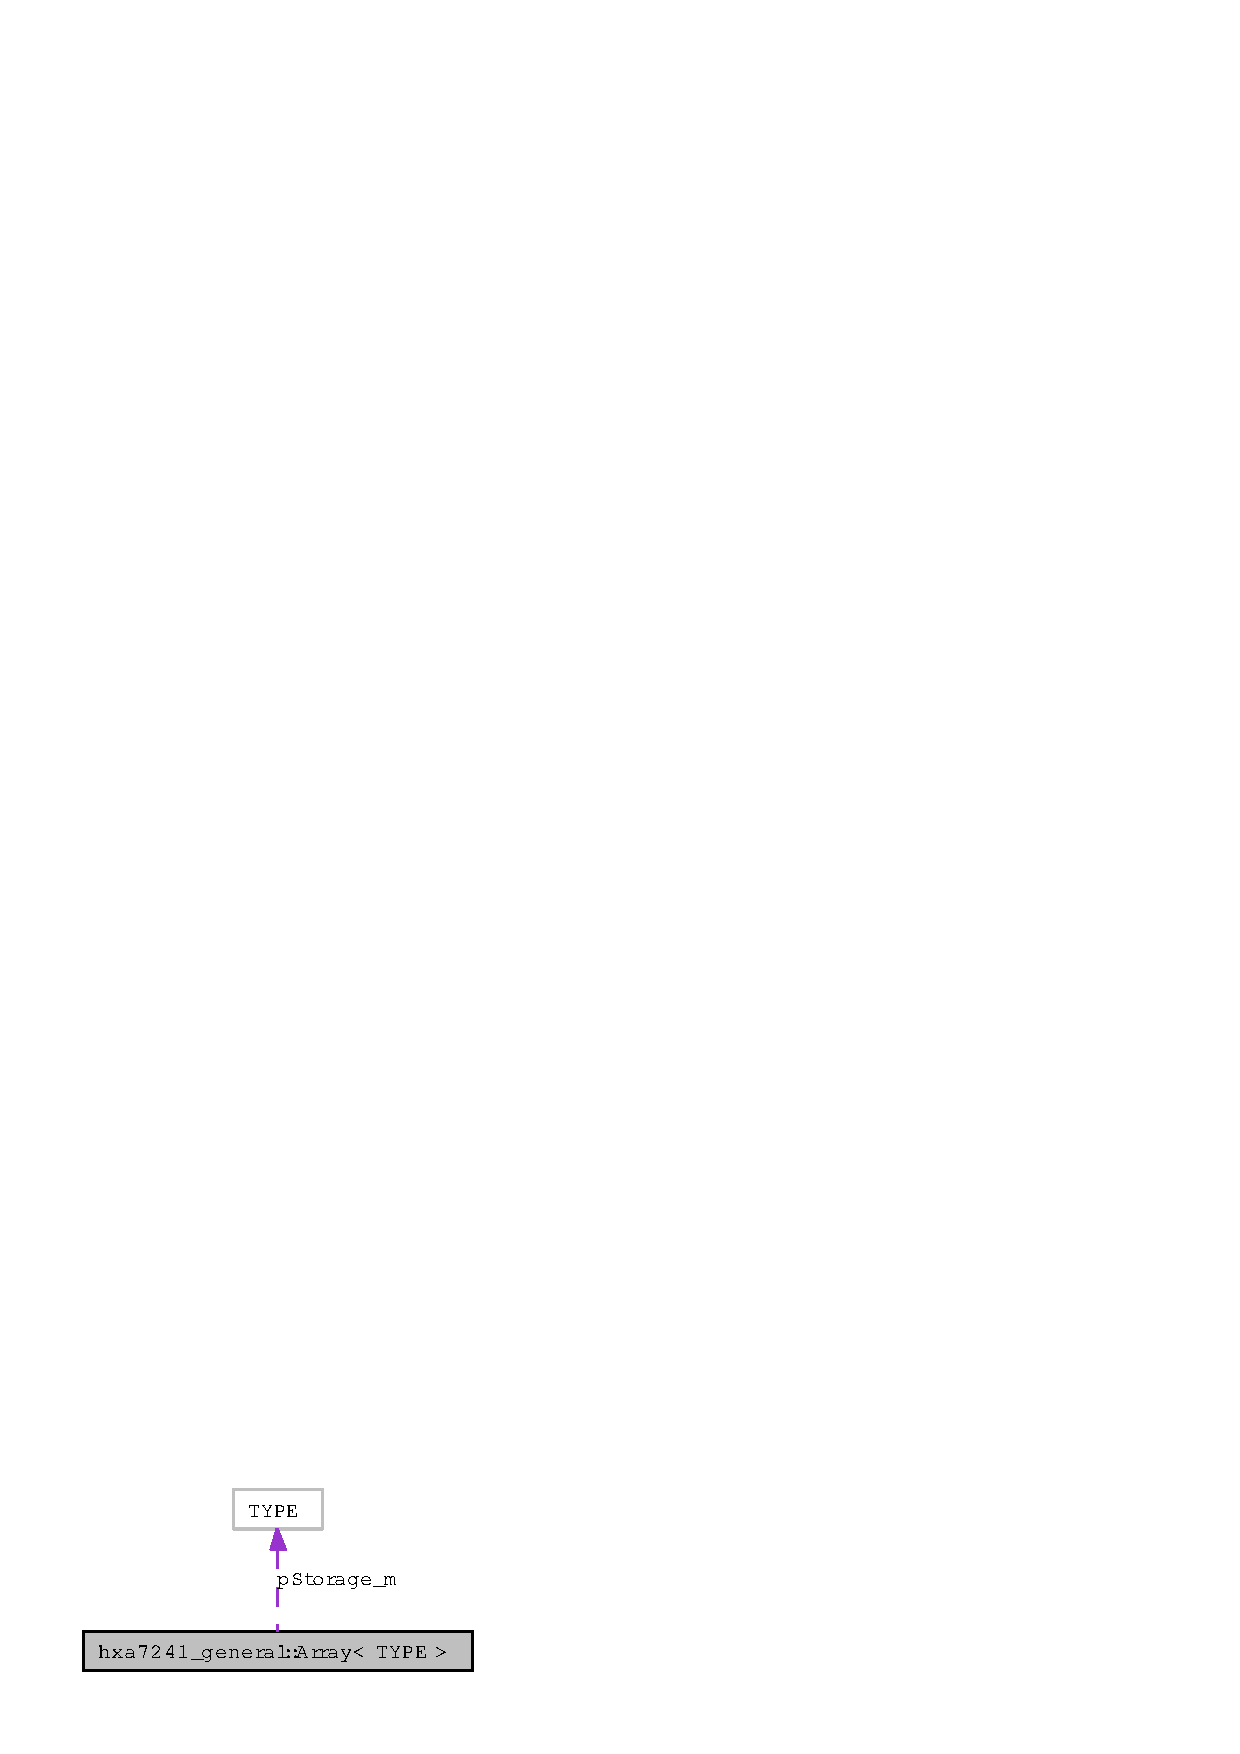
\includegraphics[width=115pt]{classhxa7241__general_1_1Array__coll__graph}
\end{center}
\end{figure}
\subsection*{Public Member Functions}
\begin{CompactItemize}
\item 
{\bf Array} ()
\begin{CompactList}\small\item\em standard object services --------------------------------------------------- \item\end{CompactList}\item 
{\bf Array} (dword length)
\item 
{\bf $\sim$Array} ()
\item 
{\bf Array} (const {\bf Array} \&)
\item 
{\bf Array} \& {\bf operator=} (const {\bf Array} \&)
\item 
void {\bf set\-Length} (dword length)
\begin{CompactList}\small\item\em commands ------------------------------------------------------------------- \item\end{CompactList}\item 
void {\bf swap} ({\bf Array} \&)
\item 
void {\bf append} (const TYPE \&)
\item 
void {\bf remove} (int index)
\item 
void {\bf zero\-Storage} ()
\item 
TYPE $\ast$ {\bf get\-Storage} ()
\item 
TYPE \& {\bf operator[$\,$]} (int index)
\item 
dword {\bf get\-Length} () const
\begin{CompactList}\small\item\em queries -------------------------------------------------------------------- \item\end{CompactList}\item 
bool {\bf is\-Empty} () const
\item 
const TYPE $\ast$ {\bf get\-Storage} () const
\item 
const TYPE \& {\bf operator[$\,$]} (int index) const
\end{CompactItemize}
\subsection*{Static Public Member Functions}
\begin{CompactItemize}
\item 
static dword {\bf get\-Max\-Length} ()
\end{CompactItemize}
\subsection*{Protected Member Functions}
\begin{CompactItemize}
\item 
void {\bf assign} (const {\bf Array}$<$ TYPE $>$ \&)
\begin{CompactList}\small\item\em implementation ------------------------------------------------------------- \item\end{CompactList}\item 
void {\bf acquire\-Storage} (dword length, bool is\-Copied)
\end{CompactItemize}
\subsection*{Static Protected Member Functions}
\begin{CompactItemize}
\item 
static void {\bf copy\-Objects} (TYPE $\ast$l\-Val\-Start, const TYPE $\ast$r\-Val\-Start, dword length)
\end{CompactItemize}


\subsection{Detailed Description}
\subsubsection*{template$<$class TYPE$>$ class hxa7241\_\-general::Array$<$ TYPE $>$}

A simpler, compacter alternative to std::vector.\par
\par


Length is explicit - there is no hidden reserve.\par
\par


$\ast$ p\-Storage\_\-m is 0 or a valid address\par
 $\ast$ length\_\-m is $>$= 0 and $<$= \doxyref{get\-Max\-Length()}{p.}{classhxa7241__general_1_1Array_d20af64d14392e5a5f6a771951721a70} (DWORD\_\-MAX)\par
 



\subsection{Constructor \& Destructor Documentation}
\index{hxa7241_general::Array@{hxa7241\_\-general::Array}!Array@{Array}}
\index{Array@{Array}!hxa7241_general::Array@{hxa7241\_\-general::Array}}
\subsubsection{\setlength{\rightskip}{0pt plus 5cm}template$<$class TYPE$>$ {\bf hxa7241\_\-general::Array}$<$ TYPE $>$::{\bf Array} ()}\label{classhxa7241__general_1_1Array_19c8ccd416430b948bece58b6ef0cd65}


standard object services --------------------------------------------------- 

\index{hxa7241_general::Array@{hxa7241\_\-general::Array}!Array@{Array}}
\index{Array@{Array}!hxa7241_general::Array@{hxa7241\_\-general::Array}}
\subsubsection{\setlength{\rightskip}{0pt plus 5cm}template$<$class TYPE$>$ {\bf hxa7241\_\-general::Array}$<$ TYPE $>$::{\bf Array} (dword {\em length})\hspace{0.3cm}{\tt  [explicit]}}\label{classhxa7241__general_1_1Array_e34427d138a69a24c3b483627d0d5825}


\index{hxa7241_general::Array@{hxa7241\_\-general::Array}!~Array@{$\sim$Array}}
\index{~Array@{$\sim$Array}!hxa7241_general::Array@{hxa7241\_\-general::Array}}
\subsubsection{\setlength{\rightskip}{0pt plus 5cm}template$<$class TYPE$>$ {\bf hxa7241\_\-general::Array}$<$ TYPE $>$::$\sim${\bf Array} ()}\label{classhxa7241__general_1_1Array_910ed166575ac746c058a54e1f50828e}


\index{hxa7241_general::Array@{hxa7241\_\-general::Array}!Array@{Array}}
\index{Array@{Array}!hxa7241_general::Array@{hxa7241\_\-general::Array}}
\subsubsection{\setlength{\rightskip}{0pt plus 5cm}template$<$class TYPE$>$ {\bf hxa7241\_\-general::Array}$<$ TYPE $>$::{\bf Array} (const {\bf Array}$<$ TYPE $>$ \&)}\label{classhxa7241__general_1_1Array_11de2e2cecf48880a62508619d7caab1}




\subsection{Member Function Documentation}
\index{hxa7241_general::Array@{hxa7241\_\-general::Array}!operator=@{operator=}}
\index{operator=@{operator=}!hxa7241_general::Array@{hxa7241\_\-general::Array}}
\subsubsection{\setlength{\rightskip}{0pt plus 5cm}template$<$class TYPE$>$ {\bf Array}$<$ TYPE $>$ \& {\bf hxa7241\_\-general::Array}$<$ TYPE $>$::operator= (const {\bf Array}$<$ TYPE $>$ \&)}\label{classhxa7241__general_1_1Array_108e643b3185767e2cc2911b62d68df2}


\index{hxa7241_general::Array@{hxa7241\_\-general::Array}!setLength@{setLength}}
\index{setLength@{setLength}!hxa7241_general::Array@{hxa7241\_\-general::Array}}
\subsubsection{\setlength{\rightskip}{0pt plus 5cm}template$<$class TYPE$>$ void {\bf hxa7241\_\-general::Array}$<$ TYPE $>$::set\-Length (dword {\em length})}\label{classhxa7241__general_1_1Array_5dca0cb17cbbe92caab48328a65ab9d4}


commands ------------------------------------------------------------------- 

\index{hxa7241_general::Array@{hxa7241\_\-general::Array}!swap@{swap}}
\index{swap@{swap}!hxa7241_general::Array@{hxa7241\_\-general::Array}}
\subsubsection{\setlength{\rightskip}{0pt plus 5cm}template$<$class TYPE$>$ void {\bf hxa7241\_\-general::Array}$<$ TYPE $>$::swap ({\bf Array}$<$ TYPE $>$ \&)}\label{classhxa7241__general_1_1Array_27f99dbdb82416aefe4ab98d61cefdc6}


\index{hxa7241_general::Array@{hxa7241\_\-general::Array}!append@{append}}
\index{append@{append}!hxa7241_general::Array@{hxa7241\_\-general::Array}}
\subsubsection{\setlength{\rightskip}{0pt plus 5cm}template$<$class TYPE$>$ void {\bf hxa7241\_\-general::Array}$<$ TYPE $>$::append (const TYPE \&)}\label{classhxa7241__general_1_1Array_6c0da347dae749198cdca92fe0974eff}


\index{hxa7241_general::Array@{hxa7241\_\-general::Array}!remove@{remove}}
\index{remove@{remove}!hxa7241_general::Array@{hxa7241\_\-general::Array}}
\subsubsection{\setlength{\rightskip}{0pt plus 5cm}template$<$class TYPE$>$ void {\bf hxa7241\_\-general::Array}$<$ TYPE $>$::remove (int {\em index})}\label{classhxa7241__general_1_1Array_df64ea9c922348d908936c9130800473}


\index{hxa7241_general::Array@{hxa7241\_\-general::Array}!zeroStorage@{zeroStorage}}
\index{zeroStorage@{zeroStorage}!hxa7241_general::Array@{hxa7241\_\-general::Array}}
\subsubsection{\setlength{\rightskip}{0pt plus 5cm}template$<$class TYPE$>$ void {\bf hxa7241\_\-general::Array}$<$ TYPE $>$::zero\-Storage ()}\label{classhxa7241__general_1_1Array_dd0d285c045512bb7d7084293a85875a}


\index{hxa7241_general::Array@{hxa7241\_\-general::Array}!getStorage@{getStorage}}
\index{getStorage@{getStorage}!hxa7241_general::Array@{hxa7241\_\-general::Array}}
\subsubsection{\setlength{\rightskip}{0pt plus 5cm}template$<$class TYPE$>$ TYPE $\ast$ {\bf hxa7241\_\-general::Array}$<$ TYPE $>$::get\-Storage ()\hspace{0.3cm}{\tt  [inline]}}\label{classhxa7241__general_1_1Array_56bd54118d903d09b4c75cc48c6a9e69}


\index{hxa7241_general::Array@{hxa7241\_\-general::Array}!operator[]@{operator[]}}
\index{operator[]@{operator[]}!hxa7241_general::Array@{hxa7241\_\-general::Array}}
\subsubsection{\setlength{\rightskip}{0pt plus 5cm}template$<$class TYPE$>$ TYPE \& {\bf hxa7241\_\-general::Array}$<$ TYPE $>$::operator[$\,$] (int {\em index})\hspace{0.3cm}{\tt  [inline]}}\label{classhxa7241__general_1_1Array_1680c1ea351c611606f8e65377f5753f}


\index{hxa7241_general::Array@{hxa7241\_\-general::Array}!getLength@{getLength}}
\index{getLength@{getLength}!hxa7241_general::Array@{hxa7241\_\-general::Array}}
\subsubsection{\setlength{\rightskip}{0pt plus 5cm}template$<$class TYPE$>$ dword {\bf hxa7241\_\-general::Array}$<$ TYPE $>$::get\-Length () const\hspace{0.3cm}{\tt  [inline]}}\label{classhxa7241__general_1_1Array_e0192970720698950334458e62244921}


queries -------------------------------------------------------------------- 

\index{hxa7241_general::Array@{hxa7241\_\-general::Array}!isEmpty@{isEmpty}}
\index{isEmpty@{isEmpty}!hxa7241_general::Array@{hxa7241\_\-general::Array}}
\subsubsection{\setlength{\rightskip}{0pt plus 5cm}template$<$class TYPE$>$ bool {\bf hxa7241\_\-general::Array}$<$ TYPE $>$::is\-Empty () const\hspace{0.3cm}{\tt  [inline]}}\label{classhxa7241__general_1_1Array_5d0848f151f59bf43f6c7e2d194e5515}


\index{hxa7241_general::Array@{hxa7241\_\-general::Array}!getMaxLength@{getMaxLength}}
\index{getMaxLength@{getMaxLength}!hxa7241_general::Array@{hxa7241\_\-general::Array}}
\subsubsection{\setlength{\rightskip}{0pt plus 5cm}template$<$class TYPE$>$ dword {\bf hxa7241\_\-general::Array}$<$ TYPE $>$::get\-Max\-Length ()\hspace{0.3cm}{\tt  [inline, static]}}\label{classhxa7241__general_1_1Array_d20af64d14392e5a5f6a771951721a70}


\index{hxa7241_general::Array@{hxa7241\_\-general::Array}!getStorage@{getStorage}}
\index{getStorage@{getStorage}!hxa7241_general::Array@{hxa7241\_\-general::Array}}
\subsubsection{\setlength{\rightskip}{0pt plus 5cm}template$<$class TYPE$>$ const TYPE $\ast$ {\bf hxa7241\_\-general::Array}$<$ TYPE $>$::get\-Storage () const\hspace{0.3cm}{\tt  [inline]}}\label{classhxa7241__general_1_1Array_9a86a5038cd279d96ca583120340a584}


\index{hxa7241_general::Array@{hxa7241\_\-general::Array}!operator[]@{operator[]}}
\index{operator[]@{operator[]}!hxa7241_general::Array@{hxa7241\_\-general::Array}}
\subsubsection{\setlength{\rightskip}{0pt plus 5cm}template$<$class TYPE$>$ const TYPE \& {\bf hxa7241\_\-general::Array}$<$ TYPE $>$::operator[$\,$] (int {\em index}) const\hspace{0.3cm}{\tt  [inline]}}\label{classhxa7241__general_1_1Array_d2489b8310652a6b58a66df9d6a6a5f8}


\index{hxa7241_general::Array@{hxa7241\_\-general::Array}!assign@{assign}}
\index{assign@{assign}!hxa7241_general::Array@{hxa7241\_\-general::Array}}
\subsubsection{\setlength{\rightskip}{0pt plus 5cm}template$<$class TYPE$>$ void {\bf hxa7241\_\-general::Array}$<$ TYPE $>$::assign (const {\bf Array}$<$ TYPE $>$ \&)\hspace{0.3cm}{\tt  [protected]}}\label{classhxa7241__general_1_1Array_ce96e08be4773e3bc1b31eaf73fce215}


implementation ------------------------------------------------------------- 

\index{hxa7241_general::Array@{hxa7241\_\-general::Array}!acquireStorage@{acquireStorage}}
\index{acquireStorage@{acquireStorage}!hxa7241_general::Array@{hxa7241\_\-general::Array}}
\subsubsection{\setlength{\rightskip}{0pt plus 5cm}template$<$class TYPE$>$ void {\bf hxa7241\_\-general::Array}$<$ TYPE $>$::acquire\-Storage (dword {\em length}, bool {\em is\-Copied})\hspace{0.3cm}{\tt  [protected]}}\label{classhxa7241__general_1_1Array_51db8453fcef1a51d478202d025fae64}


\index{hxa7241_general::Array@{hxa7241\_\-general::Array}!copyObjects@{copyObjects}}
\index{copyObjects@{copyObjects}!hxa7241_general::Array@{hxa7241\_\-general::Array}}
\subsubsection{\setlength{\rightskip}{0pt plus 5cm}template$<$class TYPE$>$ void {\bf hxa7241\_\-general::Array}$<$ TYPE $>$::copy\-Objects (TYPE $\ast$ {\em l\-Val\-Start}, const TYPE $\ast$ {\em r\-Val\-Start}, dword {\em length})\hspace{0.3cm}{\tt  [static, protected]}}\label{classhxa7241__general_1_1Array_050e82ca928bcda017ce73b3682f768e}




The documentation for this class was generated from the following file:\begin{CompactItemize}
\item 
{\bf Array.h}\end{CompactItemize}

\section{Complex Struct Reference}
\label{structComplex}\index{Complex@{Complex}}
{\tt \#include $<$container.h$>$}

Collaboration diagram for Complex:\begin{figure}[H]
\begin{center}
\leavevmode
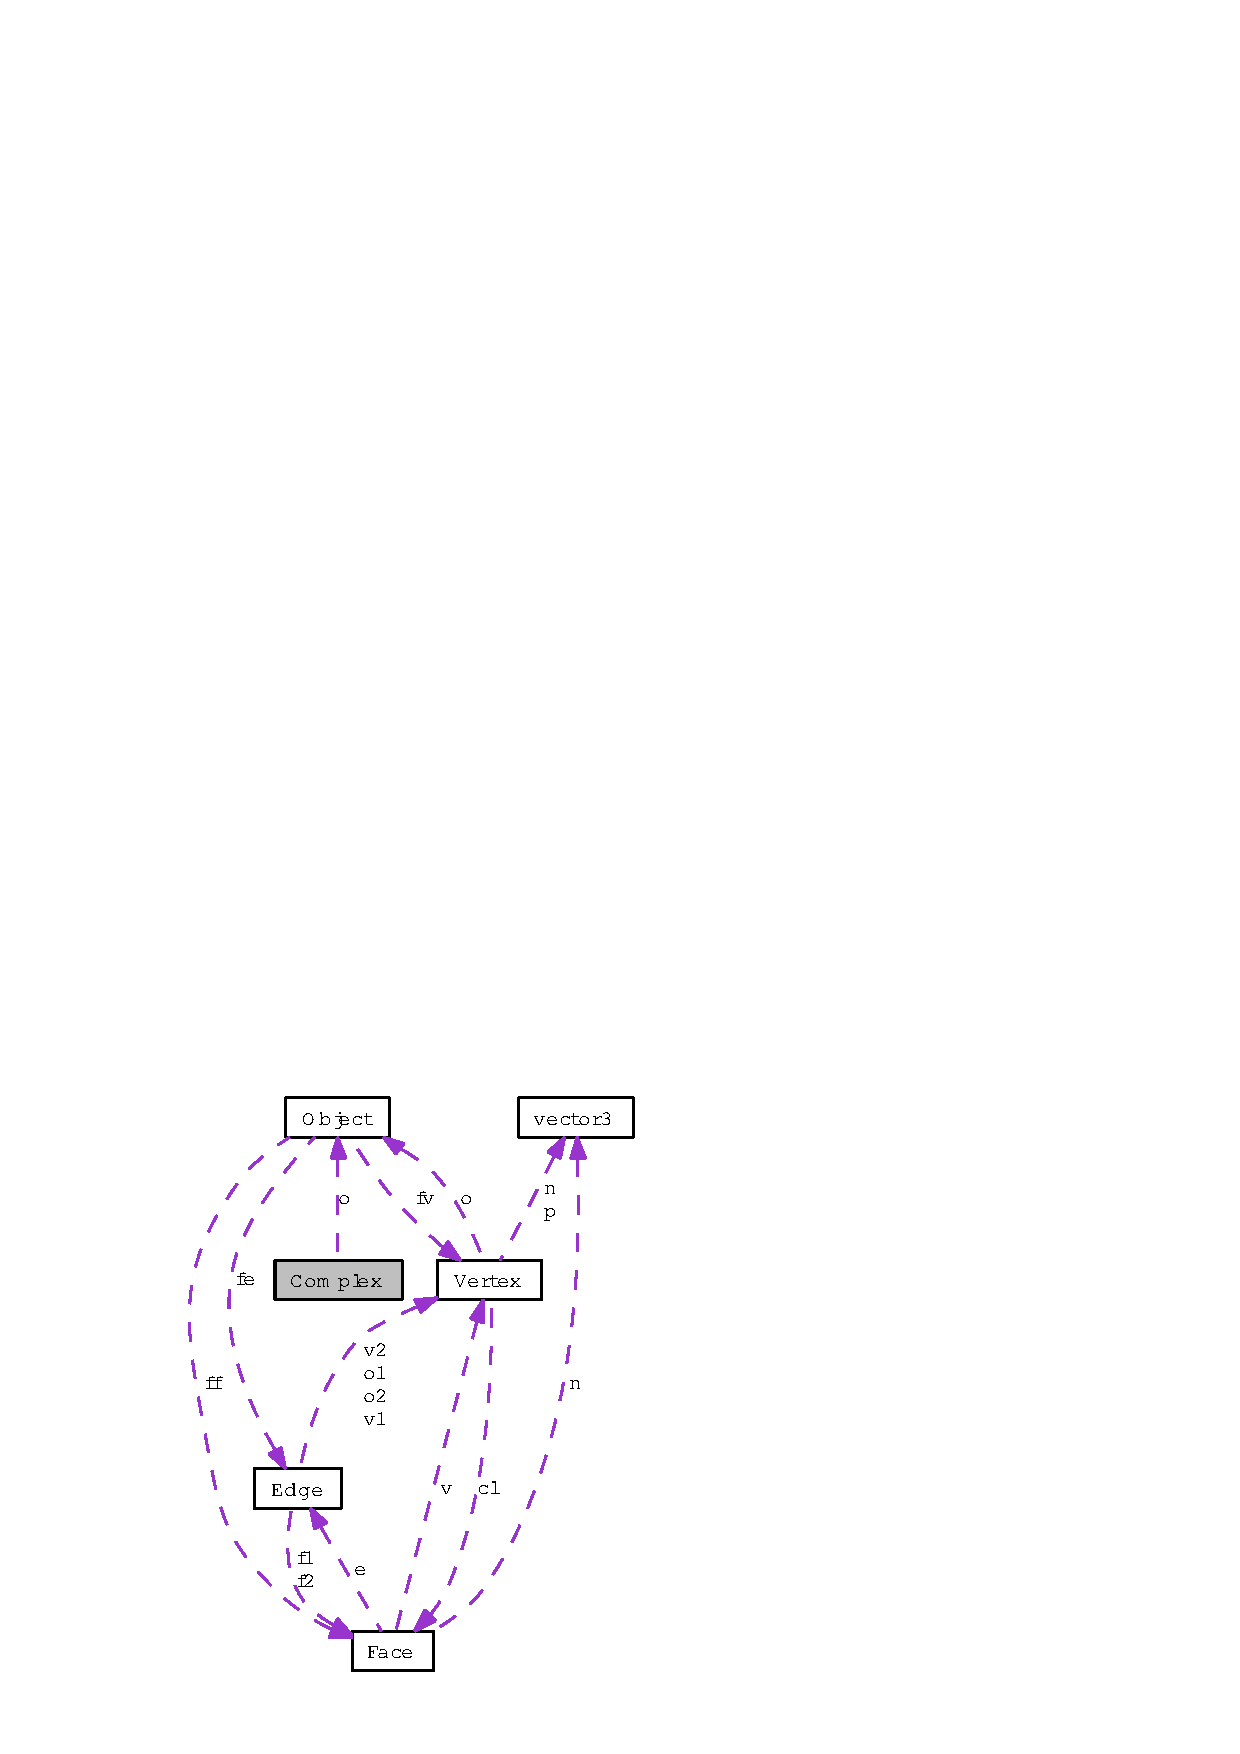
\includegraphics[width=153pt]{structComplex__coll__graph}
\end{center}
\end{figure}
\subsection*{Public Member Functions}
\begin{CompactItemize}
\item 
{\bf Complex} ({\bf Object} $\ast$oo, int i)
\end{CompactItemize}
\subsection*{Public Attributes}
\begin{CompactItemize}
\item 
{\bf Object} $\ast$ {\bf o}
\item 
int {\bf index}
\end{CompactItemize}


\subsection{Constructor \& Destructor Documentation}
\index{Complex@{Complex}!Complex@{Complex}}
\index{Complex@{Complex}!Complex@{Complex}}
\subsubsection{\setlength{\rightskip}{0pt plus 5cm}Complex::Complex ({\bf Object} $\ast$ {\em oo}, int {\em i})\hspace{0.3cm}{\tt  [inline]}}\label{structComplex_c7f33e27fa07f516f3584c40531a0818}




\subsection{Member Data Documentation}
\index{Complex@{Complex}!o@{o}}
\index{o@{o}!Complex@{Complex}}
\subsubsection{\setlength{\rightskip}{0pt plus 5cm}{\bf Object}$\ast$ {\bf Complex::o}}\label{structComplex_8f85f8797081817b2029fd94f40d5de2}


\index{Complex@{Complex}!index@{index}}
\index{index@{index}!Complex@{Complex}}
\subsubsection{\setlength{\rightskip}{0pt plus 5cm}int {\bf Complex::index}}\label{structComplex_03af76523c5ced4e5e709f54e3869fb6}




The documentation for this struct was generated from the following file:\begin{CompactItemize}
\item 
{\bf container.h}\end{CompactItemize}

\section{Container Class Reference}
\label{classContainer}\index{Container@{Container}}
{\tt \#include $<$container.h$>$}

Collaboration diagram for Container:\begin{figure}[H]
\begin{center}
\leavevmode
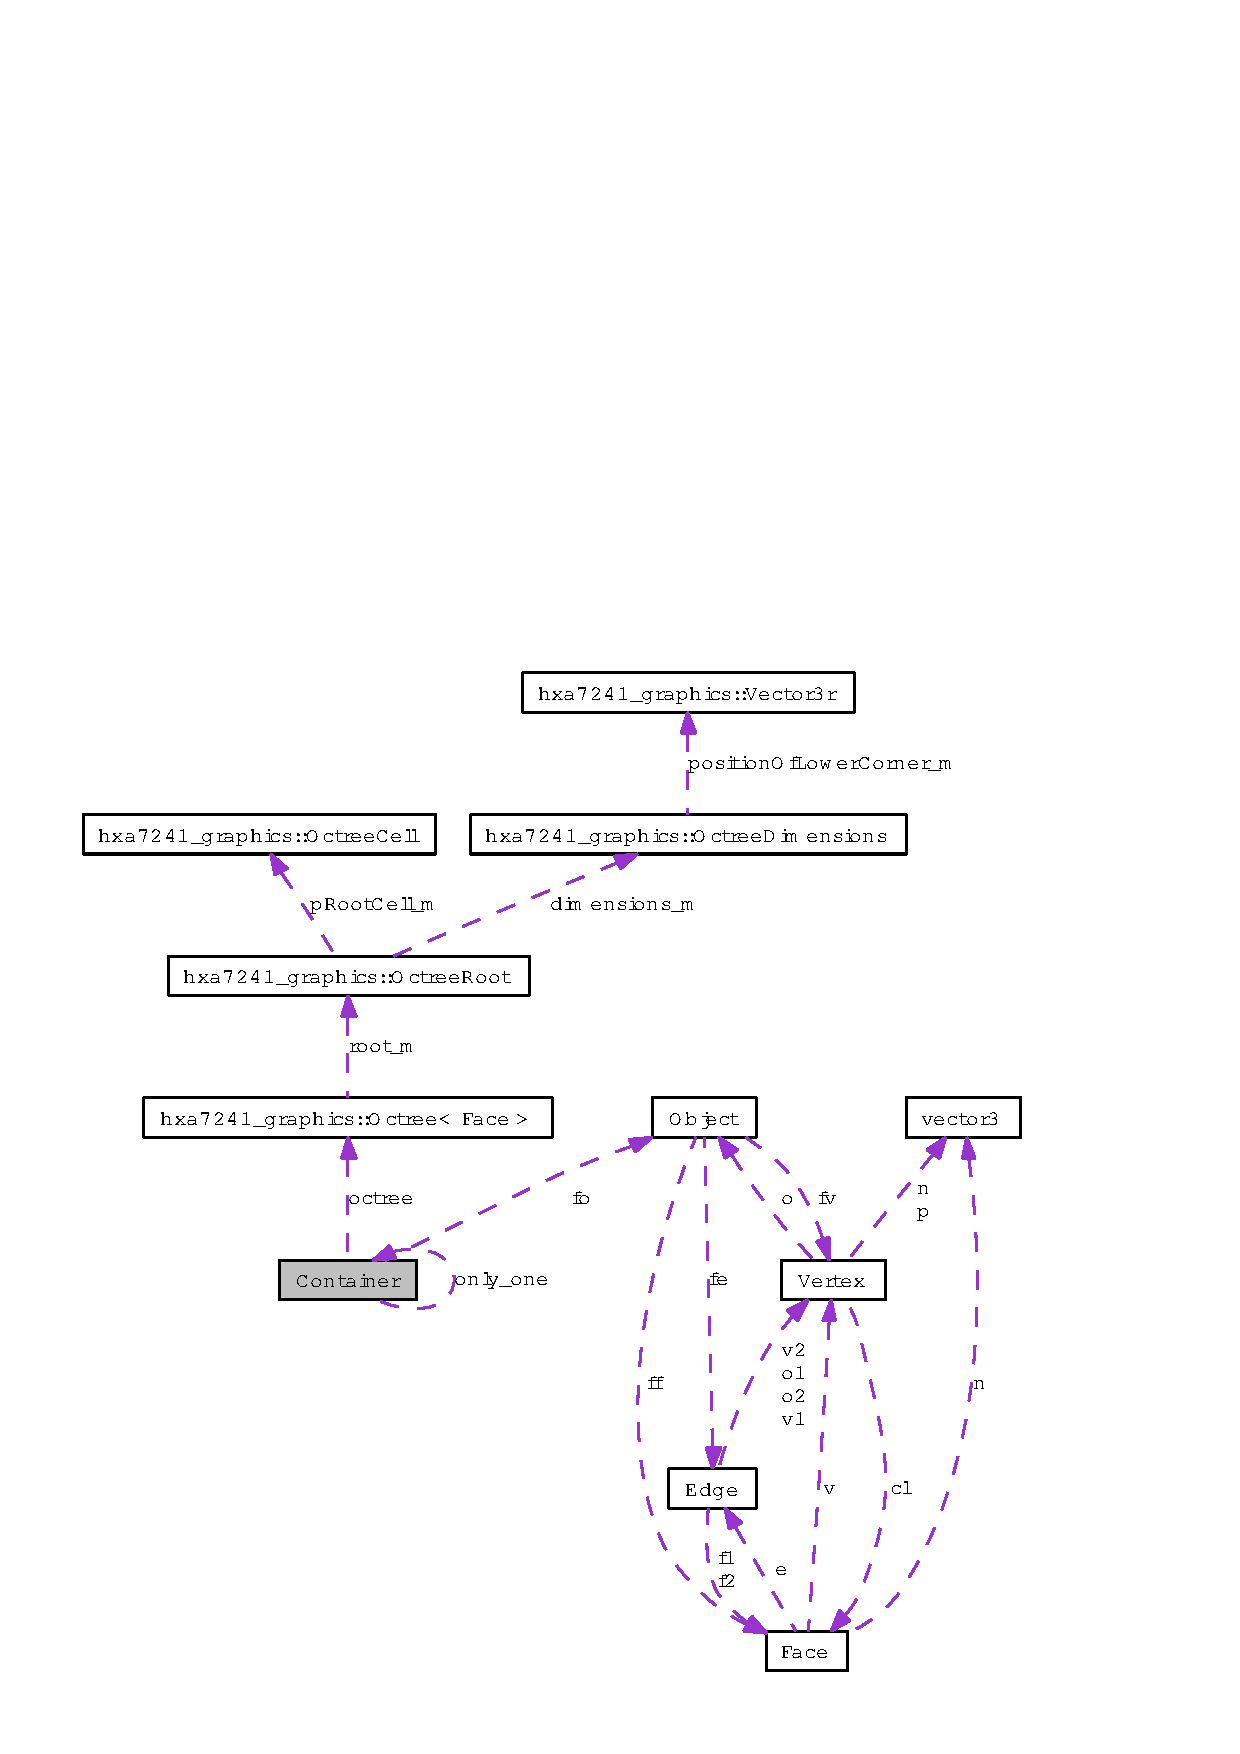
\includegraphics[width=246pt]{classContainer__coll__graph}
\end{center}
\end{figure}
\subsection*{Public Member Functions}
\begin{CompactItemize}
\item 
int {\bf get\-Vertex\-Count} (void) const
\item 
int {\bf get\-Face\-Count} (void) const
\item 
int {\bf get\-Edge\-Count} (void) const
\item 
void {\bf bound\-World} (void)
\item 
void {\bf write\-Summary} (std::ostream \&)
\item 
void {\bf scan\-Dir} (void)
\item 
void {\bf scan\-Files} (void)
\item 
void {\bf assess\-File} ({\bf Object} $\ast$const, char const $\ast$)
\item 
void {\bf scan\-File} ({\bf Object} $\ast$const, char const $\ast$)
\item 
void {\bf compute\-Vertex\-Normals} (void)
\item 
void {\bf create\-Edges} (void)
\item 
void {\bf find\-Vert\-Adj} (void)
\item 
void {\bf read\-Frozen} (char const $\ast$)
\item 
void {\bf sort\-Adjacent\-Faces} (void)
\item 
void {\bf deleteme\_\-check\-Closest\-Face} (int const \&, int const \&, std::string)
\item 
void {\bf check\-Closest\-Face} (int const \&, std::string)
\item 
void {\bf check\-Closest\-Face2} (int const \&, std::string)
\item 
void {\bf check\-Closest\-Face3} (int const \&, std::string)
\item 
void {\bf check\-Faces} (std::string)
\item 
void {\bf check\-Faces\-In\-Octree} (void)
\item 
void {\bf print\-Region\-In\-Octree} (void)
\item 
void {\bf write\-Mesh\-Data} (int const \&) const 
\item 
void {\bf find\-Closest\-Face\-To\-Each\-Vertex} (void)
\item 
void {\bf find\-Closest\-Pt\-In\-Face\-To\-Location} ({\bf vector3} const \&pt, {\bf Face} const $\ast$const face, {\bf vector3} \&p, double \&square\-D) const
\item 
void {\bf find\-Pt\-In\-Face\-Where\-Normal\-Int} ({\bf vector3} const \&pt, {\bf vector3} n, double const \&, {\bf Face} const $\ast$const face, {\bf vector3} \&p, double \&square\-D) const
\item 
bool {\bf face\-Lies\-Opposite\-To\-Normal} ({\bf vector3} const \&, {\bf Face} const $\ast$const face, {\bf vector3} const \&n) const 
\item 
bool {\bf bounding\-Box\-Fully\-In\-Search\-Region} ({\bf vec\_\-d} const \&sr, {\bf vec\_\-d} const \&bb) const
\item 
bool {\bf vertex\-Outside\-Octree\-Bounds} ({\bf vector3} const $\ast$const new\_\-pos)
\item 
bool {\bf closest\-Pt\-Is\-In\-Search\-Cone} ({\bf vector3} const \&pt, {\bf vector3} const \&p, {\bf vector3} const \&n, double const \&) const
\item 
bool {\bf find\-Closest\-Pt\-To\-Barycenter\-Among\-Faces} ({\bf vector3} const \&, {\bf Face} $\ast$const f, {\bf fp\_\-cit}, {\bf fp\_\-cit}, double const \&cone\_\-radius, {\bf vector3} \&, double \&, {\bf Face} $\ast$\&, int \&) const
\item 
bool {\bf find\-Closest\-Pt\-To\-Vertex\-Among\-Faces} ({\bf Vertex} const $\ast$const, {\bf fp\_\-cit}, {\bf fp\_\-cit}, double const \&, {\bf vector3} \&, double \&, {\bf Face} $\ast$\&, int \&) const
\item 
bool {\bf find\-Closest\-Pt\-To\-Vertex} ({\bf Vertex} const $\ast$const, {\bf vector3} \&, double \&, {\bf Face} $\ast$\&) const
\item 
bool {\bf find\-Closest\-Pt\-To\-Barycenter} ({\bf vector3} const \&pt, {\bf Face} $\ast$const f, {\bf vector3} \&, double \&, {\bf Face} $\ast$\&) const
\item 
double {\bf get\-Min\-Edge\-Angle} (void) const
\item 
double {\bf get\-World} (int const \&) const 
\item 
{\bf vec\_\-d} {\bf get\-Spherical\-Cone\-Bounding\-Box} ({\bf vector3} const \&pt, {\bf vector3} n, double const \&cone\_\-radius) const
\item 
{\bf mmap\_\-oi} {\bf load\-Map} (char const $\ast$, {\bf s\_\-set} \&)
\item 
{\bf Object} $\ast$ {\bf get\-Object\-Pointer} (std::string) const 
\item 
std::vector$<$ {\bf Complex} $>$ {\bf load\-Vector} (const char $\ast$filename, {\bf s\_\-set} \&not\_\-found)
\item 
bool {\bf vertex\-Is\-Frozen} ({\bf Vertex} $\ast$const v) const
\item 
int {\bf get\-File\-Count} (void) const
\end{CompactItemize}
\subsection*{Static Public Member Functions}
\begin{CompactItemize}
\item 
static {\bf Container} \& {\bf instance} (void)
\end{CompactItemize}
\subsection*{Public Attributes}
\begin{CompactItemize}
\item 
{\bf hxa7241\_\-graphics::Octree}$<$ {\bf Face} $>$ $\ast$ {\bf octree}
\item 
{\bf vec\_\-o} {\bf o}
\end{CompactItemize}


\subsection{Member Function Documentation}
\index{Container@{Container}!instance@{instance}}
\index{instance@{instance}!Container@{Container}}
\subsubsection{\setlength{\rightskip}{0pt plus 5cm}{\bf Container} \& Container::instance (void)\hspace{0.3cm}{\tt  [static]}}\label{classContainer_e4646d7b418a9b302db245f074ad8ec5}


\index{Container@{Container}!getVertexCount@{getVertexCount}}
\index{getVertexCount@{getVertexCount}!Container@{Container}}
\subsubsection{\setlength{\rightskip}{0pt plus 5cm}int Container::get\-Vertex\-Count (void) const}\label{classContainer_31f05695581593644aafa457cc2b2bc8}


Get the total number of vertices in the input data. \begin{Desc}
\item[Returns:]The total number of vertices in the input data. \end{Desc}
\index{Container@{Container}!getFaceCount@{getFaceCount}}
\index{getFaceCount@{getFaceCount}!Container@{Container}}
\subsubsection{\setlength{\rightskip}{0pt plus 5cm}int Container::get\-Face\-Count (void) const}\label{classContainer_570049d28d9b59a6b314fdbe9978f056}


Get the total number of faces in the input data. \begin{Desc}
\item[Returns:]The total number of faces in the input data. \end{Desc}
\index{Container@{Container}!getEdgeCount@{getEdgeCount}}
\index{getEdgeCount@{getEdgeCount}!Container@{Container}}
\subsubsection{\setlength{\rightskip}{0pt plus 5cm}int Container::get\-Edge\-Count (void) const}\label{classContainer_c805cd419c41dbc672b081b88bcb6552}


Get the total number of edges in the input data. \begin{Desc}
\item[Returns:]The total number of edges in the input data. \end{Desc}
\index{Container@{Container}!boundWorld@{boundWorld}}
\index{boundWorld@{boundWorld}!Container@{Container}}
\subsubsection{\setlength{\rightskip}{0pt plus 5cm}void Container::bound\-World (void)}\label{classContainer_a5fc905c668cc9f7909b9bbcf5beee65}


Calculate and record limits of model along each prinicpal axis. \index{Container@{Container}!writeSummary@{writeSummary}}
\index{writeSummary@{writeSummary}!Container@{Container}}
\subsubsection{\setlength{\rightskip}{0pt plus 5cm}void Container::write\-Summary (std::ostream \& {\em target})}\label{classContainer_a4e9a37eb14178872c1b735aed195eda}


Write description and summary of this class to output stream. \begin{Desc}
\item[Parameters:]
\begin{description}
\item[\mbox{$\leftarrow$} {\em target}]Pre-initialized output stream. \end{description}
\end{Desc}
\index{Container@{Container}!scanDir@{scanDir}}
\index{scanDir@{scanDir}!Container@{Container}}
\subsubsection{\setlength{\rightskip}{0pt plus 5cm}void Container::scan\-Dir (void)}\label{classContainer_e49ee77c3921f10fcc057f61b307251b}


Find all .mesh files in input directory. \index{Container@{Container}!scanFiles@{scanFiles}}
\index{scanFiles@{scanFiles}!Container@{Container}}
\subsubsection{\setlength{\rightskip}{0pt plus 5cm}void Container::scan\-Files (void)}\label{classContainer_d46293c789ebc22aa77b938b85979800}


For each .mesh file found in input directory build an instance of object class.

\begin{Desc}
\item[Returns:]Void. \end{Desc}
\index{Container@{Container}!assessFile@{assessFile}}
\index{assessFile@{assessFile}!Container@{Container}}
\subsubsection{\setlength{\rightskip}{0pt plus 5cm}void Container::assess\-File ({\bf Object} $\ast$ const {\em obj}, char const $\ast$ {\em filename})}\label{classContainer_06befe7555d878137526e7eddd1feec3}


Scan input data file once to count total number of vertices and faces in the object. \begin{Desc}
\item[Parameters:]
\begin{description}
\item[\mbox{$\leftarrow$} {\em obj}]Pointer to parent \doxyref{Object}{p.}{classObject}. \item[\mbox{$\leftarrow$} {\em filename}]Input file name. \end{description}
\end{Desc}
\index{Container@{Container}!scanFile@{scanFile}}
\index{scanFile@{scanFile}!Container@{Container}}
\subsubsection{\setlength{\rightskip}{0pt plus 5cm}void Container::scan\-File ({\bf Object} $\ast$ const {\em obj}, char const $\ast$ {\em filename})}\label{classContainer_1f2ebe727eb7f5d77f77ff9f8e60f339}


Build \doxyref{Object}{p.}{classObject} from input file data. \begin{Desc}
\item[Parameters:]
\begin{description}
\item[\mbox{$\leftarrow$} {\em obj}]Pointer to parent \doxyref{Object}{p.}{classObject}. \item[\mbox{$\leftarrow$} {\em filename}]Input file name. \end{description}
\end{Desc}
\index{Container@{Container}!computeVertexNormals@{computeVertexNormals}}
\index{computeVertexNormals@{computeVertexNormals}!Container@{Container}}
\subsubsection{\setlength{\rightskip}{0pt plus 5cm}void Container::compute\-Vertex\-Normals (void)}\label{classContainer_b103cc06097fab5f1a7204572d7c60c5}


Calculate and record the normal vector of each vertex in the model. \index{Container@{Container}!createEdges@{createEdges}}
\index{createEdges@{createEdges}!Container@{Container}}
\subsubsection{\setlength{\rightskip}{0pt plus 5cm}void Container::create\-Edges (void)}\label{classContainer_4ea77ab7f90acdf56e51e04ddef48808}


For each object build instance of edge class using face and vertex class data. \index{Container@{Container}!findVertAdj@{findVertAdj}}
\index{findVertAdj@{findVertAdj}!Container@{Container}}
\subsubsection{\setlength{\rightskip}{0pt plus 5cm}void Container::find\-Vert\-Adj (void)}\label{classContainer_3406171e70819424f595b04e4c37efc9}


For each vertex in each object add pointers to adjacent faces of vertex to vertex class. \index{Container@{Container}!readFrozen@{readFrozen}}
\index{readFrozen@{readFrozen}!Container@{Container}}
\subsubsection{\setlength{\rightskip}{0pt plus 5cm}void Container::read\-Frozen (char const $\ast$ {\em filename})}\label{classContainer_e63666838eb9afa04f2a54fdec3820f0}


Process frozen vertex data. \begin{Desc}
\item[Parameters:]
\begin{description}
\item[\mbox{$\leftarrow$} {\em filename}]Frozen vertex file name. \end{description}
\end{Desc}
\index{Container@{Container}!sortAdjacentFaces@{sortAdjacentFaces}}
\index{sortAdjacentFaces@{sortAdjacentFaces}!Container@{Container}}
\subsubsection{\setlength{\rightskip}{0pt plus 5cm}void Container::sort\-Adjacent\-Faces (void)}\label{classContainer_a91178ecc1710c316c27f54ed0ede0a9}


Sort adjacent faces of each vertex in model. \index{Container@{Container}!deleteme_checkClosestFace@{deleteme\_\-checkClosestFace}}
\index{deleteme_checkClosestFace@{deleteme\_\-checkClosestFace}!Container@{Container}}
\subsubsection{\setlength{\rightskip}{0pt plus 5cm}void Container::deleteme\_\-check\-Closest\-Face (int const \&, int const \&, std::string)}\label{classContainer_b88ab4f62ffb44dcc2db6650fe405dce}


\index{Container@{Container}!checkClosestFace@{checkClosestFace}}
\index{checkClosestFace@{checkClosestFace}!Container@{Container}}
\subsubsection{\setlength{\rightskip}{0pt plus 5cm}void Container::check\-Closest\-Face (int const \& {\em group}, std::string {\em suffix})}\label{classContainer_5350a46003ff8160b0125a6058c7603c}


Find the closest face of each vertex in container and compare with closest face stored in vertex class.

\begin{Desc}
\item[Parameters:]
\begin{description}
\item[\mbox{$\leftarrow$} {\em group}]Number of group of vertices being moved. \item[\mbox{$\leftarrow$} {\em suffix}]String to append to file name to identify when in the program the file was written. \end{description}
\end{Desc}
\index{Container@{Container}!checkClosestFace2@{checkClosestFace2}}
\index{checkClosestFace2@{checkClosestFace2}!Container@{Container}}
\subsubsection{\setlength{\rightskip}{0pt plus 5cm}void Container::check\-Closest\-Face2 (int const \&, std::string)}\label{classContainer_bebf935e5f2bcbfa593861a88693aa1e}


\index{Container@{Container}!checkClosestFace3@{checkClosestFace3}}
\index{checkClosestFace3@{checkClosestFace3}!Container@{Container}}
\subsubsection{\setlength{\rightskip}{0pt plus 5cm}void Container::check\-Closest\-Face3 (int const \&, std::string)}\label{classContainer_063be9bc92dbc325ac5911550da8a8e9}


\index{Container@{Container}!checkFaces@{checkFaces}}
\index{checkFaces@{checkFaces}!Container@{Container}}
\subsubsection{\setlength{\rightskip}{0pt plus 5cm}void Container::check\-Faces (std::string {\em s})}\label{classContainer_35bf9908f07f7a95a44af9878d41629f}


Check that all faces have flag set to false. \begin{Desc}
\item[Parameters:]
\begin{description}
\item[\mbox{$\leftarrow$} {\em s}]Error message if face found with flag set to true. \end{description}
\end{Desc}
\index{Container@{Container}!checkFacesInOctree@{checkFacesInOctree}}
\index{checkFacesInOctree@{checkFacesInOctree}!Container@{Container}}
\subsubsection{\setlength{\rightskip}{0pt plus 5cm}void Container::check\-Faces\-In\-Octree (void)}\label{classContainer_2b2598775cc2a322fc7ded1d7a54f899}


Check that all faces are present in appropriate octree cells. \index{Container@{Container}!printRegionInOctree@{printRegionInOctree}}
\index{printRegionInOctree@{printRegionInOctree}!Container@{Container}}
\subsubsection{\setlength{\rightskip}{0pt plus 5cm}void Container::print\-Region\-In\-Octree (void)}\label{classContainer_4b1cfa76345dbe77dd8b2b04bb742eee}


Print octree overlapping region. \index{Container@{Container}!writeMeshData@{writeMeshData}}
\index{writeMeshData@{writeMeshData}!Container@{Container}}
\subsubsection{\setlength{\rightskip}{0pt plus 5cm}void Container::write\-Mesh\-Data (int const \& {\em group}) const}\label{classContainer_a1c33ec2055ed34432ee1deb355e8930}


Write to file the current position of all mesh objects. \begin{Desc}
\item[Parameters:]
\begin{description}
\item[\mbox{$\leftarrow$} {\em group}]The current group number from \doxyref{meshmorph.cc}{p.}{meshmorph_8cc}. \end{description}
\end{Desc}
\index{Container@{Container}!findClosestFaceToEachVertex@{findClosestFaceToEachVertex}}
\index{findClosestFaceToEachVertex@{findClosestFaceToEachVertex}!Container@{Container}}
\subsubsection{\setlength{\rightskip}{0pt plus 5cm}void Container::find\-Closest\-Face\-To\-Each\-Vertex (void)}\label{classContainer_ba37bd114f68b67a78dc4c09e8029abb}


Find and record the closest face to each vertex in the model. \index{Container@{Container}!findClosestPtInFaceToLocation@{findClosestPtInFaceToLocation}}
\index{findClosestPtInFaceToLocation@{findClosestPtInFaceToLocation}!Container@{Container}}
\subsubsection{\setlength{\rightskip}{0pt plus 5cm}void Container::find\-Closest\-Pt\-In\-Face\-To\-Location ({\bf vector3} const \& {\em pt}, {\bf Face} const $\ast$const {\em face}, {\bf vector3} \& {\em closest\_\-point}, double \& {\em f\-Sqr\-Distance}) const}\label{classContainer_837dbd3229fe0507a940cec75883405c}


Find closest point in face to input location.

\begin{Desc}
\item[Parameters:]
\begin{description}
\item[\mbox{$\leftarrow$} {\em pt}]Location of interest. \item[\mbox{$\leftarrow$} {\em face}]\doxyref{Face}{p.}{classFace} on which closest point to input location will be identified. \item[\mbox{$\rightarrow$} {\em closest\_\-point}]Closest point position, if found. \item[\mbox{$\rightarrow$} {\em f\-Sqr\-Distance}]Squared distance between input location and closest point, if found. \end{description}
\end{Desc}
\begin{Desc}
\item[Returns:]True if closest point found; otherwise false. \end{Desc}
\index{Container@{Container}!findPtInFaceWhereNormalInt@{findPtInFaceWhereNormalInt}}
\index{findPtInFaceWhereNormalInt@{findPtInFaceWhereNormalInt}!Container@{Container}}
\subsubsection{\setlength{\rightskip}{0pt plus 5cm}void Container::find\-Pt\-In\-Face\-Where\-Normal\-Int ({\bf vector3} const \& {\em pt}, {\bf vector3} {\em n}, double const \& {\em cone\_\-radius}, {\bf Face} const $\ast$const {\em face}, {\bf vector3} \& {\em intersection\_\-point}, double \& {\em f\-Sqr\-Distance}) const}\label{classContainer_abfb5b26e0d1018db39bb5994645c2c7}


Find intersection point of vertex normal vector and input face.

\begin{Desc}
\item[Parameters:]
\begin{description}
\item[\mbox{$\leftarrow$} {\em pt}]Location of interest. \item[\mbox{$\leftarrow$} {\em face}]\doxyref{Face}{p.}{classFace} on which intersection point of normal vector will be identified. \item[\mbox{$\rightarrow$} {\em intersection\_\-point}]Intersection point position, if found. \item[\mbox{$\rightarrow$} {\em f\-Sqr\-Distance}]Squared distance between input location and intersection point, if found. \end{description}
\end{Desc}
\begin{Desc}
\item[Returns:]True if intersection point found; otherwise false. \end{Desc}
\index{Container@{Container}!faceLiesOppositeToNormal@{faceLiesOppositeToNormal}}
\index{faceLiesOppositeToNormal@{faceLiesOppositeToNormal}!Container@{Container}}
\subsubsection{\setlength{\rightskip}{0pt plus 5cm}bool Container::face\-Lies\-Opposite\-To\-Normal ({\bf vector3} const \& {\em pt}, {\bf Face} const $\ast$const {\em face}, {\bf vector3} const \& {\em nn}) const}\label{classContainer_d1d134db6575e05a59b9d1e553a37db1}


Determine if entire input face lies in hemispace opposite to normal vector at input location. \begin{Desc}
\item[Parameters:]
\begin{description}
\item[\mbox{$\leftarrow$} {\em pt}]Location of interest. \item[\mbox{$\leftarrow$} {\em face}]\doxyref{Face}{p.}{classFace} of interest. \item[\mbox{$\leftarrow$} {\em nn}]Normal vector of this face. \end{description}
\end{Desc}
\begin{Desc}
\item[Returns:]True if entire face lies opposite to normal vector; false otherwise. \end{Desc}
\index{Container@{Container}!boundingBoxFullyInSearchRegion@{boundingBoxFullyInSearchRegion}}
\index{boundingBoxFullyInSearchRegion@{boundingBoxFullyInSearchRegion}!Container@{Container}}
\subsubsection{\setlength{\rightskip}{0pt plus 5cm}bool Container::bounding\-Box\-Fully\-In\-Search\-Region ({\bf vec\_\-d} const \& {\em sr}, {\bf vec\_\-d} const \& {\em bb}) const}\label{classContainer_f6c9062691e697dbc3a36066b70094a6}


Determine if input bounding box is fully inside the input search region. \begin{Desc}
\item[Parameters:]
\begin{description}
\item[\mbox{$\leftarrow$} {\em sr}]Search region [xmin,xmax,ymin,ymax,zmin,zmax]. \item[\mbox{$\leftarrow$} {\em bb}]Bounding box [xmin,xmax,ymin,ymax,zmin,zmax]. \end{description}
\end{Desc}
\begin{Desc}
\item[Returns:]True if bounding box is fully inside search region; false otherwise. \end{Desc}
\index{Container@{Container}!vertexOutsideOctreeBounds@{vertexOutsideOctreeBounds}}
\index{vertexOutsideOctreeBounds@{vertexOutsideOctreeBounds}!Container@{Container}}
\subsubsection{\setlength{\rightskip}{0pt plus 5cm}bool Container::vertex\-Outside\-Octree\-Bounds ({\bf vector3} const $\ast$const  {\em new\_\-pos})}\label{classContainer_44faaf0d36151e1bef4e82167ff56c36}


Check if moved vertex has breached octree boundary.

\begin{Desc}
\item[Parameters:]
\begin{description}
\item[\mbox{$\leftarrow$} {\em new\_\-pos}]The new position of current vertex. \end{description}
\end{Desc}
\begin{Desc}
\item[Returns:]True if vertex has moved to a location outside of octree bounday, false otherwise. \end{Desc}
\index{Container@{Container}!closestPtIsInSearchCone@{closestPtIsInSearchCone}}
\index{closestPtIsInSearchCone@{closestPtIsInSearchCone}!Container@{Container}}
\subsubsection{\setlength{\rightskip}{0pt plus 5cm}bool Container::closest\-Pt\-Is\-In\-Search\-Cone ({\bf vector3} const \& {\em pt}, {\bf vector3} const \& {\em p}, {\bf vector3} const \& {\em n}, double const \& {\em sqd\_\-sep\_\-dist}) const}\label{classContainer_565ad9f08462161c38360f7f3b16f3d9}


Determine if closest point is inside search cone. \begin{Desc}
\item[Parameters:]
\begin{description}
\item[\mbox{$\leftarrow$} {\em pt}]Point of interest. \item[\mbox{$\leftarrow$} {\em p}]Closest point of interest. \item[\mbox{$\leftarrow$} {\em n}]\doxyref{Vertex}{p.}{classVertex} normal vector. \item[\mbox{$\leftarrow$} {\em sqd\_\-sep\_\-dist}]Squared distance between point and vertex. \end{description}
\end{Desc}
\begin{Desc}
\item[Returns:]True if point is inside vertex search cone; false otherwise; \end{Desc}
\index{Container@{Container}!findClosestPtToBarycenterAmongFaces@{findClosestPtToBarycenterAmongFaces}}
\index{findClosestPtToBarycenterAmongFaces@{findClosestPtToBarycenterAmongFaces}!Container@{Container}}
\subsubsection{\setlength{\rightskip}{0pt plus 5cm}bool Container::find\-Closest\-Pt\-To\-Barycenter\-Among\-Faces ({\bf vector3} const \& {\em pt}, {\bf Face} $\ast$const  {\em f}, {\bf fp\_\-cit} {\em begin}, {\bf fp\_\-cit} {\em end}, double const \& {\em cone\_\-radius}, {\bf vector3} \& {\em p}, double \& {\em square\-D}, {\bf Face} $\ast$\& {\em ncl}, int \& {\em faces\_\-checked}) const}\label{classContainer_91bf3d22d0a3ce63c3bb80bab6946e35}


Find closest point to tile's barycenter among input faces. \begin{Desc}
\item[Parameters:]
\begin{description}
\item[\mbox{$\leftarrow$} {\em pt}]Barycenter of face tile for which closest point is searched. \item[\mbox{$\leftarrow$} {\em f}]\doxyref{Face}{p.}{classFace} on which tile is located. \item[\mbox{$\leftarrow$} {\em begin}]Iterator pointing to first face in vector of faces to check. \item[\mbox{$\leftarrow$} {\em end}]Iterator pointing to one past the last face in vector of faces to check. \item[\mbox{$\rightarrow$} {\em p}]Closest point position, if found. \item[\mbox{$\rightarrow$} {\em square\-D}]Squared distance between vertex and closest point, if found. \item[\mbox{$\rightarrow$} {\em ncl}]Parent face of closest point, if found. \item[\mbox{$\rightarrow$} {\em faces\_\-checked}]Cumulative number of faces checked. \end{description}
\end{Desc}
\begin{Desc}
\item[Returns:]True if closest point found; otherwise false. \end{Desc}
\index{Container@{Container}!findClosestPtToVertexAmongFaces@{findClosestPtToVertexAmongFaces}}
\index{findClosestPtToVertexAmongFaces@{findClosestPtToVertexAmongFaces}!Container@{Container}}
\subsubsection{\setlength{\rightskip}{0pt plus 5cm}bool Container::find\-Closest\-Pt\-To\-Vertex\-Among\-Faces ({\bf Vertex} const $\ast$ const {\em v}, {\bf fp\_\-cit} {\em begin}, {\bf fp\_\-cit} {\em end}, double const \& {\em cone\_\-radius}, {\bf vector3} \& {\em p}, double \& {\em square\-D}, {\bf Face} $\ast$\& {\em ncl}, int \& {\em faces\_\-checked}) const}\label{classContainer_4d781e1e289f742adf6e71a632de530c}


Find closest point to vertex among input faces.

\begin{Desc}
\item[Parameters:]
\begin{description}
\item[\mbox{$\leftarrow$} {\em v}]\doxyref{Vertex}{p.}{classVertex} of interest. \item[\mbox{$\leftarrow$} {\em begin}]Iterator pointing to first face in vector of faces to check. \item[\mbox{$\leftarrow$} {\em end}]Iterator pointing to one past the last face in vector of faces to check. \item[\mbox{$\rightarrow$} {\em p}]Closest point position, if found. \item[\mbox{$\rightarrow$} {\em square\-D}]Squared distance between vertex and closest point, if found. \item[\mbox{$\rightarrow$} {\em ncl}]Parent face of closest point, if found. \item[\mbox{$\rightarrow$} {\em faces\_\-checked}]Cumulative number of faces checked. \end{description}
\end{Desc}
\begin{Desc}
\item[Returns:]True if closest point found; otherwise false. \end{Desc}
\index{Container@{Container}!findClosestPtToVertex@{findClosestPtToVertex}}
\index{findClosestPtToVertex@{findClosestPtToVertex}!Container@{Container}}
\subsubsection{\setlength{\rightskip}{0pt plus 5cm}bool Container::find\-Closest\-Pt\-To\-Vertex ({\bf Vertex} const $\ast$ const {\em v}, {\bf vector3} \& {\em p}, double \& {\em sqd}, {\bf Face} $\ast$\& {\em ncl}) const}\label{classContainer_6ff5eef4c44b9e539b0fafd6cd3951c0}


Find the closest point to a vertex. \begin{Desc}
\item[Parameters:]
\begin{description}
\item[\mbox{$\leftarrow$} {\em v}]\doxyref{Vertex}{p.}{classVertex} for which closest point is searched. \item[\mbox{$\rightarrow$} {\em p}]Closest point position, if found. \item[\mbox{$\rightarrow$} {\em sqd}]Squared distance between vertex and closest point, if found. \item[\mbox{$\rightarrow$} {\em ncl}]Parent face of closest point, if found. \end{description}
\end{Desc}
\begin{Desc}
\item[Returns:]True if closest point found; otherwise false. \end{Desc}
\index{Container@{Container}!findClosestPtToBarycenter@{findClosestPtToBarycenter}}
\index{findClosestPtToBarycenter@{findClosestPtToBarycenter}!Container@{Container}}
\subsubsection{\setlength{\rightskip}{0pt plus 5cm}bool Container::find\-Closest\-Pt\-To\-Barycenter ({\bf vector3} const \& {\em pt}, {\bf Face} $\ast$const  {\em f}, {\bf vector3} \& {\em p}, double \& {\em sqd}, {\bf Face} $\ast$\& {\em ncl}) const}\label{classContainer_6a3bb520f8dbcf3fedda302851ca1574}


Find the closest point to a tile's barycenter. \begin{Desc}
\item[Parameters:]
\begin{description}
\item[\mbox{$\leftarrow$} {\em pt}]Barycenter of face tile for which closest point is searched. \item[\mbox{$\leftarrow$} {\em f}]\doxyref{Face}{p.}{classFace} on which tile is located. \item[\mbox{$\rightarrow$} {\em p}]Closest point position, if found. \item[\mbox{$\rightarrow$} {\em sqd}]Squared distance between barycenter and closest point, if found. \item[\mbox{$\rightarrow$} {\em ncl}]Parent face of closest point, if found. \end{description}
\end{Desc}
\begin{Desc}
\item[Returns:]True if closest point found; otherwise false. \end{Desc}
\index{Container@{Container}!getMinEdgeAngle@{getMinEdgeAngle}}
\index{getMinEdgeAngle@{getMinEdgeAngle}!Container@{Container}}
\subsubsection{\setlength{\rightskip}{0pt plus 5cm}double Container::get\-Min\-Edge\-Angle (void) const}\label{classContainer_05aadd9612e660c318188c1bb6d08168}


Find the edge in model with smallest angle and return angle. \begin{Desc}
\item[Returns:]Smallest edge angle in radians. \end{Desc}
\index{Container@{Container}!getWorld@{getWorld}}
\index{getWorld@{getWorld}!Container@{Container}}
\subsubsection{\setlength{\rightskip}{0pt plus 5cm}double Container::get\-World (int const \& {\em axis}) const}\label{classContainer_52f51ec2336524ab9dee6e34bbaf5817}


Return the world limit along input axis. \begin{Desc}
\item[Parameters:]
\begin{description}
\item[\mbox{$\leftarrow$} {\em axis}]Requested direction 0,1,2,3,4,5 == -x,+x,-y,+y,-z,+z. \end{description}
\end{Desc}
\begin{Desc}
\item[Returns:]World limit along ith axis. \end{Desc}
\index{Container@{Container}!getSphericalConeBoundingBox@{getSphericalConeBoundingBox}}
\index{getSphericalConeBoundingBox@{getSphericalConeBoundingBox}!Container@{Container}}
\subsubsection{\setlength{\rightskip}{0pt plus 5cm}{\bf vec\_\-d} Container::get\-Spherical\-Cone\-Bounding\-Box ({\bf vector3} const \& {\em pt}, {\bf vector3} {\em n}, double const \& {\em cone\_\-radius}) const}\label{classContainer_61686822f39e2081f28e55b4588575df}


Compute axis-aligned bounding box of spherical cone. \begin{Desc}
\item[Parameters:]
\begin{description}
\item[\mbox{$\leftarrow$} {\em pt}]Point of interest. \item[\mbox{$\leftarrow$} {\em n}]Normal vector at point of interest. \item[\mbox{$\leftarrow$} {\em cone\_\-radius}]Spherical cone radius. \end{description}
\end{Desc}
\begin{Desc}
\item[Returns:]Bounding box along principal axes [xmin,xmax,ymin,ymax,zmin,zmax]. \end{Desc}
\index{Container@{Container}!loadMap@{loadMap}}
\index{loadMap@{loadMap}!Container@{Container}}
\subsubsection{\setlength{\rightskip}{0pt plus 5cm}{\bf mmap\_\-oi} Container::load\-Map (char const $\ast$, {\bf s\_\-set} \&)}\label{classContainer_411e568e6df9c842916a57e81bf7b18c}


\index{Container@{Container}!getObjectPointer@{getObjectPointer}}
\index{getObjectPointer@{getObjectPointer}!Container@{Container}}
\subsubsection{\setlength{\rightskip}{0pt plus 5cm}{\bf Object} $\ast$ Container::get\-Object\-Pointer (std::string {\em name}) const}\label{classContainer_73fa40d6071c9bec7535f17cc1e605e7}


Get pointer to object with matching name. \begin{Desc}
\item[Parameters:]
\begin{description}
\item[\mbox{$\leftarrow$} {\em name}]Name of object of interest. \end{description}
\end{Desc}
\begin{Desc}
\item[Returns:]Pointer to object with name that matches the input name; otherwise NULL. \end{Desc}
\index{Container@{Container}!loadVector@{loadVector}}
\index{loadVector@{loadVector}!Container@{Container}}
\subsubsection{\setlength{\rightskip}{0pt plus 5cm}std::vector$<$ {\bf Complex} $>$ Container::load\-Vector (const char $\ast$ {\em filename}, {\bf s\_\-set} \& {\em not\_\-found})}\label{classContainer_2bddb5801b2a1b80d19974184405a452}


Parse input file of vertices (obejct name and vertex index) and store data. \begin{Desc}
\item[Parameters:]
\begin{description}
\item[\mbox{$\leftarrow$} {\em filename}]Input file name. \item[\mbox{$\rightarrow$} {\em not\_\-found}]Set of object names from file that were not found in input data. \end{description}
\end{Desc}
\begin{Desc}
\item[Returns:]Stored object data. \end{Desc}
\index{Container@{Container}!vertexIsFrozen@{vertexIsFrozen}}
\index{vertexIsFrozen@{vertexIsFrozen}!Container@{Container}}
\subsubsection{\setlength{\rightskip}{0pt plus 5cm}bool Container::vertex\-Is\-Frozen ({\bf Vertex} $\ast$const {\em v}) const\hspace{0.3cm}{\tt  [inline]}}\label{classContainer_18d7d38743a6da8e383f6d59280066d0}


Check if vertex is frozen. \begin{Desc}
\item[Parameters:]
\begin{description}
\item[\mbox{$\leftarrow$} {\em v}]\doxyref{Vertex}{p.}{classVertex} of interest. \end{description}
\end{Desc}
\begin{Desc}
\item[Returns:]True if vertex is frozen; otherwise false; \end{Desc}
\index{Container@{Container}!getFileCount@{getFileCount}}
\index{getFileCount@{getFileCount}!Container@{Container}}
\subsubsection{\setlength{\rightskip}{0pt plus 5cm}int Container::get\-File\-Count (void) const\hspace{0.3cm}{\tt  [inline]}}\label{classContainer_b5b53af75606a8358b48efdea451227f}


Get number of input mesh files. \begin{Desc}
\item[Returns:]Number of input files. \end{Desc}


\subsection{Member Data Documentation}
\index{Container@{Container}!octree@{octree}}
\index{octree@{octree}!Container@{Container}}
\subsubsection{\setlength{\rightskip}{0pt plus 5cm}{\bf hxa7241\_\-graphics::Octree}$<${\bf Face}$>$$\ast$ {\bf Container::octree}}\label{classContainer_4df52f9f8477885e34143f8e5dffec8d}


\index{Container@{Container}!o@{o}}
\index{o@{o}!Container@{Container}}
\subsubsection{\setlength{\rightskip}{0pt plus 5cm}{\bf vec\_\-o} {\bf Container::o}}\label{classContainer_c3ac0ef8e13fb01215064cd9bd24ff85}




The documentation for this class was generated from the following files:\begin{CompactItemize}
\item 
{\bf container.h}\item 
{\bf container.cc}\end{CompactItemize}

\hypertarget{classControls}{
\section{Controls Class Reference}
\label{classControls}\index{Controls@{Controls}}
}
{\tt \#include $<$controls.h$>$}

\subsection*{Public Member Functions}
\begin{CompactItemize}
\item 
void \hyperlink{classControls_c155d57ffffad8062dca68e5dd8e45c1}{parseCommandLine} (int, char $\ast$$\ast$)
\item 
std::string \hyperlink{classControls_cc10201b6a7efde6066fd29e797abaf4}{getUsageMessage} (void)
\item 
int \hyperlink{classControls_b7738197e6e7658acde1e73bf6519c41}{getNumReserve} () const   throw ()
\item 
int \hyperlink{classControls_718c293ec502518db33c8491e8ef84db}{getCappingFlag} () const   throw ()
\item 
int \hyperlink{classControls_5f70bbd62a41dd74fee9750acf432a19}{getMinSection} () const   throw ()
\item 
int \hyperlink{classControls_afc35dff6349419fe3b0089c78a56127}{getMaxSection} () const   throw ()
\item 
int \hyperlink{classControls_fb69cf3fe723123d382dbf709ece5f84}{getPrintDetailedInfo} () const   throw ()
\item 
int \hyperlink{classControls_7d717253ec34914ab2643b463777f72d}{getReturnRawContourPoints} () const   throw ()
\item 
int \hyperlink{classControls_96dac19dcb0a887e9e3f49c663bb5709}{getReturnInterpolatedRawPoints} () const   throw ()
\item 
int \hyperlink{classControls_4ba998e75d7c20623b65863de139aecf}{getPtPerContourThreshold} () const   throw ()
\item 
int \hyperlink{classControls_a3748a625808c17247692cd9c8d5ca4c}{getNumMovesPerIteration} () const   throw ()
\item 
int \hyperlink{classControls_c1bb853f9584201b07822e6c44e73f1a}{getMaxNumMoveAttempts} () const   throw ()
\item 
int \hyperlink{classControls_68df257c4251022461ab172c787d5242}{getIntegrationStep} () const   throw ()
\item 
int \hyperlink{classControls_26ba220025ff09c85dcdf9f8b6321b99}{getMaxDeviationAdjustments} () const   throw ()
\item 
int \hyperlink{classControls_5876b02a1eb372a76525bba36a39ea34}{getCurvatureEnergyExponent} () const   throw ()
\item 
int \hyperlink{classControls_79da34adf73fe0098834c2e801f36fd5}{getProximityEnergyExponent} () const   throw ()
\item 
double \hyperlink{classControls_556e825aa9766b9349c68cad370562f0}{getAdditionalPointsFactor} () const   throw ()
\item 
double \hyperlink{classControls_c939bf45ea4c27a61f73fc3f4ad01107}{getIntegrationStepFactor} () const   throw ()
\item 
double \hyperlink{classControls_060a80a65cbb830e71c0edce3cb837a3}{getHighTemp} () const   throw ()
\item 
double \hyperlink{classControls_2a6718effb5b99b4bacc07e2c274a371}{getTempScale} () const   throw ()
\item 
double \hyperlink{classControls_c185f29a09bb9eb583ecd9bf4324f217}{getBoltzman} () const   throw ()
\item 
double \hyperlink{classControls_821c182631d0e65f2262f2824e8f1f1a}{getCurvatureEnergyGain} () const   throw ()
\item 
double \hyperlink{classControls_c07acead6db3d81b104d2604d599660e}{getProximityEnergyGain} () const   throw ()
\item 
double \hyperlink{classControls_68ea9d72317226e8c95e60dc40a6beb6}{getMeanAmplitudeNoise} () const   throw ()
\item 
double \hyperlink{classControls_48e342e9425d94235ec8a73002815268}{getMaxRadiusOfCurvature} () const   throw ()
\item 
double \hyperlink{classControls_066ed1d2f58c990a3d269df94f65b553}{getSectionThickness} () const   throw ()
\item 
double \hyperlink{classControls_04ccfec20fdc596a900c95088f364fa8}{getOutputScaleFactor} () const   throw ()
\item 
double \hyperlink{classControls_fc84e06f47e14332d587027d319f8fee}{getDeviationThreshold} () const   throw ()
\item 
double \hyperlink{classControls_3d5b9e235d3459dfc1e2af8e02cd7b64}{getEpsilon} () const   throw ()
\item 
double \hyperlink{classControls_98f1837fca9b50d4cee7fa8b2c296572}{getMaxSampleInterval} () const   throw ()
\item 
double \hyperlink{classControls_bafd5f43ca67322425ef272c2f91542d}{getMinSampleInterval} () const   throw ()
\item 
char const $\ast$ \hyperlink{classControls_a81627abb77cefffc5e08c0bd1d2ae8d}{getInputDir} () const   throw ()
\item 
char const $\ast$ \hyperlink{classControls_fa588b8bd920e905787ea6965cc57c91}{getOutputDir} () const   throw ()
\item 
char const $\ast$ \hyperlink{classControls_441d81822ecacabee389d0c042775b96}{getPrefix} () const   throw ()
\item 
char const $\ast$ \hyperlink{classControls_552dbe0a3a05ede218a2fc8b21ce8c3b}{getOutputScript} () const   throw ()
\item 
char const $\ast$ \hyperlink{classControls_acd1a231f7b7df8ed6341a0807221a55}{getMultiPartSuffix} () const   throw ()
\item 
void \hyperlink{classControls_b73d68f47510bc7098ebe4a636c613ce}{validate} (void)
\item 
bool \hyperlink{classControls_3ea8c4351e489235cb411d50798185b6}{contourIsIgnored} (char const $\ast$const name) const 
\item 
std::string \hyperlink{classControls_77c3bc1e6a73f2d3df39e773e2dc1ea8}{d2str} (double const \&num) const 
\item 
std::string \hyperlink{classControls_c90675a41d4cce28524cb6b929d8cc11}{i2str} (int const \&num) const 
\item 
std::string \hyperlink{classControls_8495fe7cdfa4cca8c820c591a99c9f8e}{processDir} (char $\ast$ptr) const 
\end{CompactItemize}
\subsection*{Static Public Member Functions}
\begin{CompactItemize}
\item 
static \hyperlink{classControls}{Controls} \& \hyperlink{classControls_39f30cbd69ccbf480c976228725e0ed3}{instance} (void)
\end{CompactItemize}


\subsection{Member Function Documentation}
\hypertarget{classControls_39f30cbd69ccbf480c976228725e0ed3}{
\index{Controls@{Controls}!instance@{instance}}
\index{instance@{instance}!Controls@{Controls}}
\subsubsection[instance]{\setlength{\rightskip}{0pt plus 5cm}{\bf Controls} \& Controls::instance (void)\hspace{0.3cm}{\tt  \mbox{[}static\mbox{]}}}}
\label{classControls_39f30cbd69ccbf480c976228725e0ed3}




Referenced by Contour::clearArcLengthsLogFiles(), Contour::clearControlLogFiles(), Container::clearOutputScripts(), Object::clearPtsFiles(), Contour::clearRadiusCurvatureLogFiles(), Contour::clearSampleLogFiles(), Contour::clearSParamLogFiles(), Contour::clearUniformSampleLogFiles(), Container::Container(), Sim\_\-Anneal::debug(), Sim\_\-Anneal::decreaseTemp(), Parameter::deviationsLarge(), distinguishable(), Contour::fewButKeep(), Contour::fewOmit(), Container::getContours(), Sim\_\-Anneal::getNormalRandom(), Parameter::getRawPointsToDuplicate(), Contour::initializeControlPointVector(), Sim\_\-Anneal::isFrozen(), main(), Sim\_\-Anneal::moreMoves(), Contour::printPtsFiles(), Object::printRawPoints(), Contour::printRawPtsFiles(), Sim\_\-Anneal::printScript(), Contour::printScripts(), Contour::printSimpleScripts(), Object::processContour(), Contour::processContour(), Object::purgeBadContours(), Contour::setSamplesToRaw(), Contour::writeFilesAfter(), and Object::writeOutputContours().\hypertarget{classControls_c155d57ffffad8062dca68e5dd8e45c1}{
\index{Controls@{Controls}!parseCommandLine@{parseCommandLine}}
\index{parseCommandLine@{parseCommandLine}!Controls@{Controls}}
\subsubsection[parseCommandLine]{\setlength{\rightskip}{0pt plus 5cm}void Controls::parseCommandLine (int {\em argc}, \/  char $\ast$$\ast$ {\em argv})}}
\label{classControls_c155d57ffffad8062dca68e5dd8e45c1}


Parse command line. \begin{Desc}
\item[Parameters:]
\begin{description}
\item[\mbox{$\leftarrow$} {\em argc}]Argc. \item[\mbox{$\leftarrow$} {\em argv}]Argv. \end{description}
\end{Desc}


References getUsageMessage(), processDir(), and validate().

Referenced by main().\hypertarget{classControls_cc10201b6a7efde6066fd29e797abaf4}{
\index{Controls@{Controls}!getUsageMessage@{getUsageMessage}}
\index{getUsageMessage@{getUsageMessage}!Controls@{Controls}}
\subsubsection[getUsageMessage]{\setlength{\rightskip}{0pt plus 5cm}std::string Controls::getUsageMessage (void)}}
\label{classControls_cc10201b6a7efde6066fd29e797abaf4}


Create usage message. \begin{Desc}
\item[Returns:]usage message. \end{Desc}


References d2str(), and i2str().

Referenced by parseCommandLine().\hypertarget{classControls_b7738197e6e7658acde1e73bf6519c41}{
\index{Controls@{Controls}!getNumReserve@{getNumReserve}}
\index{getNumReserve@{getNumReserve}!Controls@{Controls}}
\subsubsection[getNumReserve]{\setlength{\rightskip}{0pt plus 5cm}int Controls::getNumReserve () const  throw ()\hspace{0.3cm}{\tt  \mbox{[}inline\mbox{]}}}}
\label{classControls_b7738197e6e7658acde1e73bf6519c41}


\hypertarget{classControls_718c293ec502518db33c8491e8ef84db}{
\index{Controls@{Controls}!getCappingFlag@{getCappingFlag}}
\index{getCappingFlag@{getCappingFlag}!Controls@{Controls}}
\subsubsection[getCappingFlag]{\setlength{\rightskip}{0pt plus 5cm}int Controls::getCappingFlag () const  throw ()\hspace{0.3cm}{\tt  \mbox{[}inline\mbox{]}}}}
\label{classControls_718c293ec502518db33c8491e8ef84db}




Referenced by Object::writeOutputContours().\hypertarget{classControls_5f70bbd62a41dd74fee9750acf432a19}{
\index{Controls@{Controls}!getMinSection@{getMinSection}}
\index{getMinSection@{getMinSection}!Controls@{Controls}}
\subsubsection[getMinSection]{\setlength{\rightskip}{0pt plus 5cm}int Controls::getMinSection () const  throw ()\hspace{0.3cm}{\tt  \mbox{[}inline\mbox{]}}}}
\label{classControls_5f70bbd62a41dd74fee9750acf432a19}




Referenced by Container::getContours().\hypertarget{classControls_afc35dff6349419fe3b0089c78a56127}{
\index{Controls@{Controls}!getMaxSection@{getMaxSection}}
\index{getMaxSection@{getMaxSection}!Controls@{Controls}}
\subsubsection[getMaxSection]{\setlength{\rightskip}{0pt plus 5cm}int Controls::getMaxSection () const  throw ()\hspace{0.3cm}{\tt  \mbox{[}inline\mbox{]}}}}
\label{classControls_afc35dff6349419fe3b0089c78a56127}




Referenced by Container::getContours().\hypertarget{classControls_fb69cf3fe723123d382dbf709ece5f84}{
\index{Controls@{Controls}!getPrintDetailedInfo@{getPrintDetailedInfo}}
\index{getPrintDetailedInfo@{getPrintDetailedInfo}!Controls@{Controls}}
\subsubsection[getPrintDetailedInfo]{\setlength{\rightskip}{0pt plus 5cm}int Controls::getPrintDetailedInfo () const  throw ()\hspace{0.3cm}{\tt  \mbox{[}inline\mbox{]}}}}
\label{classControls_fb69cf3fe723123d382dbf709ece5f84}




Referenced by main(), Object::processContour(), Contour::processContour(), and Object::writeOutputContours().\hypertarget{classControls_7d717253ec34914ab2643b463777f72d}{
\index{Controls@{Controls}!getReturnRawContourPoints@{getReturnRawContourPoints}}
\index{getReturnRawContourPoints@{getReturnRawContourPoints}!Controls@{Controls}}
\subsubsection[getReturnRawContourPoints]{\setlength{\rightskip}{0pt plus 5cm}int Controls::getReturnRawContourPoints () const  throw ()\hspace{0.3cm}{\tt  \mbox{[}inline\mbox{]}}}}
\label{classControls_7d717253ec34914ab2643b463777f72d}


\hypertarget{classControls_96dac19dcb0a887e9e3f49c663bb5709}{
\index{Controls@{Controls}!getReturnInterpolatedRawPoints@{getReturnInterpolatedRawPoints}}
\index{getReturnInterpolatedRawPoints@{getReturnInterpolatedRawPoints}!Controls@{Controls}}
\subsubsection[getReturnInterpolatedRawPoints]{\setlength{\rightskip}{0pt plus 5cm}int Controls::getReturnInterpolatedRawPoints () const  throw ()\hspace{0.3cm}{\tt  \mbox{[}inline\mbox{]}}}}
\label{classControls_96dac19dcb0a887e9e3f49c663bb5709}




Referenced by Contour::initializeControlPointVector().\hypertarget{classControls_4ba998e75d7c20623b65863de139aecf}{
\index{Controls@{Controls}!getPtPerContourThreshold@{getPtPerContourThreshold}}
\index{getPtPerContourThreshold@{getPtPerContourThreshold}!Controls@{Controls}}
\subsubsection[getPtPerContourThreshold]{\setlength{\rightskip}{0pt plus 5cm}int Controls::getPtPerContourThreshold () const  throw ()\hspace{0.3cm}{\tt  \mbox{[}inline\mbox{]}}}}
\label{classControls_4ba998e75d7c20623b65863de139aecf}




Referenced by Contour::fewButKeep(), Contour::fewOmit(), Object::processContour(), and Object::purgeBadContours().\hypertarget{classControls_a3748a625808c17247692cd9c8d5ca4c}{
\index{Controls@{Controls}!getNumMovesPerIteration@{getNumMovesPerIteration}}
\index{getNumMovesPerIteration@{getNumMovesPerIteration}!Controls@{Controls}}
\subsubsection[getNumMovesPerIteration]{\setlength{\rightskip}{0pt plus 5cm}int Controls::getNumMovesPerIteration () const  throw ()\hspace{0.3cm}{\tt  \mbox{[}inline\mbox{]}}}}
\label{classControls_a3748a625808c17247692cd9c8d5ca4c}




Referenced by Sim\_\-Anneal::debug(), and Sim\_\-Anneal::moreMoves().\hypertarget{classControls_c1bb853f9584201b07822e6c44e73f1a}{
\index{Controls@{Controls}!getMaxNumMoveAttempts@{getMaxNumMoveAttempts}}
\index{getMaxNumMoveAttempts@{getMaxNumMoveAttempts}!Controls@{Controls}}
\subsubsection[getMaxNumMoveAttempts]{\setlength{\rightskip}{0pt plus 5cm}int Controls::getMaxNumMoveAttempts () const  throw ()\hspace{0.3cm}{\tt  \mbox{[}inline\mbox{]}}}}
\label{classControls_c1bb853f9584201b07822e6c44e73f1a}




Referenced by Sim\_\-Anneal::debug(), and Sim\_\-Anneal::moreMoves().\hypertarget{classControls_68df257c4251022461ab172c787d5242}{
\index{Controls@{Controls}!getIntegrationStep@{getIntegrationStep}}
\index{getIntegrationStep@{getIntegrationStep}!Controls@{Controls}}
\subsubsection[getIntegrationStep]{\setlength{\rightskip}{0pt plus 5cm}int Controls::getIntegrationStep () const  throw ()\hspace{0.3cm}{\tt  \mbox{[}inline\mbox{]}}}}
\label{classControls_68df257c4251022461ab172c787d5242}


\hypertarget{classControls_26ba220025ff09c85dcdf9f8b6321b99}{
\index{Controls@{Controls}!getMaxDeviationAdjustments@{getMaxDeviationAdjustments}}
\index{getMaxDeviationAdjustments@{getMaxDeviationAdjustments}!Controls@{Controls}}
\subsubsection[getMaxDeviationAdjustments]{\setlength{\rightskip}{0pt plus 5cm}int Controls::getMaxDeviationAdjustments () const  throw ()\hspace{0.3cm}{\tt  \mbox{[}inline\mbox{]}}}}
\label{classControls_26ba220025ff09c85dcdf9f8b6321b99}


\hypertarget{classControls_5876b02a1eb372a76525bba36a39ea34}{
\index{Controls@{Controls}!getCurvatureEnergyExponent@{getCurvatureEnergyExponent}}
\index{getCurvatureEnergyExponent@{getCurvatureEnergyExponent}!Controls@{Controls}}
\subsubsection[getCurvatureEnergyExponent]{\setlength{\rightskip}{0pt plus 5cm}int Controls::getCurvatureEnergyExponent () const  throw ()\hspace{0.3cm}{\tt  \mbox{[}inline\mbox{]}}}}
\label{classControls_5876b02a1eb372a76525bba36a39ea34}


\hypertarget{classControls_79da34adf73fe0098834c2e801f36fd5}{
\index{Controls@{Controls}!getProximityEnergyExponent@{getProximityEnergyExponent}}
\index{getProximityEnergyExponent@{getProximityEnergyExponent}!Controls@{Controls}}
\subsubsection[getProximityEnergyExponent]{\setlength{\rightskip}{0pt plus 5cm}int Controls::getProximityEnergyExponent () const  throw ()\hspace{0.3cm}{\tt  \mbox{[}inline\mbox{]}}}}
\label{classControls_79da34adf73fe0098834c2e801f36fd5}


\hypertarget{classControls_556e825aa9766b9349c68cad370562f0}{
\index{Controls@{Controls}!getAdditionalPointsFactor@{getAdditionalPointsFactor}}
\index{getAdditionalPointsFactor@{getAdditionalPointsFactor}!Controls@{Controls}}
\subsubsection[getAdditionalPointsFactor]{\setlength{\rightskip}{0pt plus 5cm}double Controls::getAdditionalPointsFactor () const  throw ()\hspace{0.3cm}{\tt  \mbox{[}inline\mbox{]}}}}
\label{classControls_556e825aa9766b9349c68cad370562f0}


\hypertarget{classControls_c939bf45ea4c27a61f73fc3f4ad01107}{
\index{Controls@{Controls}!getIntegrationStepFactor@{getIntegrationStepFactor}}
\index{getIntegrationStepFactor@{getIntegrationStepFactor}!Controls@{Controls}}
\subsubsection[getIntegrationStepFactor]{\setlength{\rightskip}{0pt plus 5cm}double Controls::getIntegrationStepFactor () const  throw ()\hspace{0.3cm}{\tt  \mbox{[}inline\mbox{]}}}}
\label{classControls_c939bf45ea4c27a61f73fc3f4ad01107}


\hypertarget{classControls_060a80a65cbb830e71c0edce3cb837a3}{
\index{Controls@{Controls}!getHighTemp@{getHighTemp}}
\index{getHighTemp@{getHighTemp}!Controls@{Controls}}
\subsubsection[getHighTemp]{\setlength{\rightskip}{0pt plus 5cm}double Controls::getHighTemp () const  throw ()\hspace{0.3cm}{\tt  \mbox{[}inline\mbox{]}}}}
\label{classControls_060a80a65cbb830e71c0edce3cb837a3}


\hypertarget{classControls_2a6718effb5b99b4bacc07e2c274a371}{
\index{Controls@{Controls}!getTempScale@{getTempScale}}
\index{getTempScale@{getTempScale}!Controls@{Controls}}
\subsubsection[getTempScale]{\setlength{\rightskip}{0pt plus 5cm}double Controls::getTempScale () const  throw ()\hspace{0.3cm}{\tt  \mbox{[}inline\mbox{]}}}}
\label{classControls_2a6718effb5b99b4bacc07e2c274a371}




Referenced by Sim\_\-Anneal::decreaseTemp().\hypertarget{classControls_c185f29a09bb9eb583ecd9bf4324f217}{
\index{Controls@{Controls}!getBoltzman@{getBoltzman}}
\index{getBoltzman@{getBoltzman}!Controls@{Controls}}
\subsubsection[getBoltzman]{\setlength{\rightskip}{0pt plus 5cm}double Controls::getBoltzman () const  throw ()\hspace{0.3cm}{\tt  \mbox{[}inline\mbox{]}}}}
\label{classControls_c185f29a09bb9eb583ecd9bf4324f217}




Referenced by Sim\_\-Anneal::decreaseTemp().\hypertarget{classControls_821c182631d0e65f2262f2824e8f1f1a}{
\index{Controls@{Controls}!getCurvatureEnergyGain@{getCurvatureEnergyGain}}
\index{getCurvatureEnergyGain@{getCurvatureEnergyGain}!Controls@{Controls}}
\subsubsection[getCurvatureEnergyGain]{\setlength{\rightskip}{0pt plus 5cm}double Controls::getCurvatureEnergyGain () const  throw ()\hspace{0.3cm}{\tt  \mbox{[}inline\mbox{]}}}}
\label{classControls_821c182631d0e65f2262f2824e8f1f1a}


\hypertarget{classControls_c07acead6db3d81b104d2604d599660e}{
\index{Controls@{Controls}!getProximityEnergyGain@{getProximityEnergyGain}}
\index{getProximityEnergyGain@{getProximityEnergyGain}!Controls@{Controls}}
\subsubsection[getProximityEnergyGain]{\setlength{\rightskip}{0pt plus 5cm}double Controls::getProximityEnergyGain () const  throw ()\hspace{0.3cm}{\tt  \mbox{[}inline\mbox{]}}}}
\label{classControls_c07acead6db3d81b104d2604d599660e}


\hypertarget{classControls_68ea9d72317226e8c95e60dc40a6beb6}{
\index{Controls@{Controls}!getMeanAmplitudeNoise@{getMeanAmplitudeNoise}}
\index{getMeanAmplitudeNoise@{getMeanAmplitudeNoise}!Controls@{Controls}}
\subsubsection[getMeanAmplitudeNoise]{\setlength{\rightskip}{0pt plus 5cm}double Controls::getMeanAmplitudeNoise () const  throw ()\hspace{0.3cm}{\tt  \mbox{[}inline\mbox{]}}}}
\label{classControls_68ea9d72317226e8c95e60dc40a6beb6}




Referenced by Sim\_\-Anneal::getNormalRandom().\hypertarget{classControls_48e342e9425d94235ec8a73002815268}{
\index{Controls@{Controls}!getMaxRadiusOfCurvature@{getMaxRadiusOfCurvature}}
\index{getMaxRadiusOfCurvature@{getMaxRadiusOfCurvature}!Controls@{Controls}}
\subsubsection[getMaxRadiusOfCurvature]{\setlength{\rightskip}{0pt plus 5cm}double Controls::getMaxRadiusOfCurvature () const  throw ()\hspace{0.3cm}{\tt  \mbox{[}inline\mbox{]}}}}
\label{classControls_48e342e9425d94235ec8a73002815268}


\hypertarget{classControls_066ed1d2f58c990a3d269df94f65b553}{
\index{Controls@{Controls}!getSectionThickness@{getSectionThickness}}
\index{getSectionThickness@{getSectionThickness}!Controls@{Controls}}
\subsubsection[getSectionThickness]{\setlength{\rightskip}{0pt plus 5cm}double Controls::getSectionThickness () const  throw ()\hspace{0.3cm}{\tt  \mbox{[}inline\mbox{]}}}}
\label{classControls_066ed1d2f58c990a3d269df94f65b553}




Referenced by Contour::printPtsFiles(), and Contour::printRawPtsFiles().\hypertarget{classControls_04ccfec20fdc596a900c95088f364fa8}{
\index{Controls@{Controls}!getOutputScaleFactor@{getOutputScaleFactor}}
\index{getOutputScaleFactor@{getOutputScaleFactor}!Controls@{Controls}}
\subsubsection[getOutputScaleFactor]{\setlength{\rightskip}{0pt plus 5cm}double Controls::getOutputScaleFactor () const  throw ()\hspace{0.3cm}{\tt  \mbox{[}inline\mbox{]}}}}
\label{classControls_04ccfec20fdc596a900c95088f364fa8}




Referenced by Contour::printPtsFiles(), and Contour::printRawPtsFiles().\hypertarget{classControls_fc84e06f47e14332d587027d319f8fee}{
\index{Controls@{Controls}!getDeviationThreshold@{getDeviationThreshold}}
\index{getDeviationThreshold@{getDeviationThreshold}!Controls@{Controls}}
\subsubsection[getDeviationThreshold]{\setlength{\rightskip}{0pt plus 5cm}double Controls::getDeviationThreshold () const  throw ()\hspace{0.3cm}{\tt  \mbox{[}inline\mbox{]}}}}
\label{classControls_fc84e06f47e14332d587027d319f8fee}




Referenced by Parameter::deviationsLarge(), and Parameter::getRawPointsToDuplicate().\hypertarget{classControls_3d5b9e235d3459dfc1e2af8e02cd7b64}{
\index{Controls@{Controls}!getEpsilon@{getEpsilon}}
\index{getEpsilon@{getEpsilon}!Controls@{Controls}}
\subsubsection[getEpsilon]{\setlength{\rightskip}{0pt plus 5cm}double Controls::getEpsilon () const  throw ()\hspace{0.3cm}{\tt  \mbox{[}inline\mbox{]}}}}
\label{classControls_3d5b9e235d3459dfc1e2af8e02cd7b64}


\hypertarget{classControls_98f1837fca9b50d4cee7fa8b2c296572}{
\index{Controls@{Controls}!getMaxSampleInterval@{getMaxSampleInterval}}
\index{getMaxSampleInterval@{getMaxSampleInterval}!Controls@{Controls}}
\subsubsection[getMaxSampleInterval]{\setlength{\rightskip}{0pt plus 5cm}double Controls::getMaxSampleInterval () const  throw ()\hspace{0.3cm}{\tt  \mbox{[}inline\mbox{]}}}}
\label{classControls_98f1837fca9b50d4cee7fa8b2c296572}


\hypertarget{classControls_bafd5f43ca67322425ef272c2f91542d}{
\index{Controls@{Controls}!getMinSampleInterval@{getMinSampleInterval}}
\index{getMinSampleInterval@{getMinSampleInterval}!Controls@{Controls}}
\subsubsection[getMinSampleInterval]{\setlength{\rightskip}{0pt plus 5cm}double Controls::getMinSampleInterval () const  throw ()\hspace{0.3cm}{\tt  \mbox{[}inline\mbox{]}}}}
\label{classControls_bafd5f43ca67322425ef272c2f91542d}


\hypertarget{classControls_a81627abb77cefffc5e08c0bd1d2ae8d}{
\index{Controls@{Controls}!getInputDir@{getInputDir}}
\index{getInputDir@{getInputDir}!Controls@{Controls}}
\subsubsection[getInputDir]{\setlength{\rightskip}{0pt plus 5cm}char const$\ast$ Controls::getInputDir () const  throw ()\hspace{0.3cm}{\tt  \mbox{[}inline\mbox{]}}}}
\label{classControls_a81627abb77cefffc5e08c0bd1d2ae8d}




Referenced by Container::getContours().\hypertarget{classControls_fa588b8bd920e905787ea6965cc57c91}{
\index{Controls@{Controls}!getOutputDir@{getOutputDir}}
\index{getOutputDir@{getOutputDir}!Controls@{Controls}}
\subsubsection[getOutputDir]{\setlength{\rightskip}{0pt plus 5cm}char const$\ast$ Controls::getOutputDir () const  throw ()\hspace{0.3cm}{\tt  \mbox{[}inline\mbox{]}}}}
\label{classControls_fa588b8bd920e905787ea6965cc57c91}




Referenced by Container::clearOutputScripts(), Object::clearPtsFiles(), Contour::printPtsFiles(), Contour::printRawPtsFiles(), Sim\_\-Anneal::printScript(), Contour::printScripts(), Contour::printSimpleScripts(), Contour::processContour(), and Contour::writeFilesAfter().\hypertarget{classControls_441d81822ecacabee389d0c042775b96}{
\index{Controls@{Controls}!getPrefix@{getPrefix}}
\index{getPrefix@{getPrefix}!Controls@{Controls}}
\subsubsection[getPrefix]{\setlength{\rightskip}{0pt plus 5cm}char const$\ast$ Controls::getPrefix () const  throw ()\hspace{0.3cm}{\tt  \mbox{[}inline\mbox{]}}}}
\label{classControls_441d81822ecacabee389d0c042775b96}




Referenced by Container::getContours().\hypertarget{classControls_552dbe0a3a05ede218a2fc8b21ce8c3b}{
\index{Controls@{Controls}!getOutputScript@{getOutputScript}}
\index{getOutputScript@{getOutputScript}!Controls@{Controls}}
\subsubsection[getOutputScript]{\setlength{\rightskip}{0pt plus 5cm}char const$\ast$ Controls::getOutputScript () const  throw ()\hspace{0.3cm}{\tt  \mbox{[}inline\mbox{]}}}}
\label{classControls_552dbe0a3a05ede218a2fc8b21ce8c3b}




Referenced by Container::clearOutputScripts().\hypertarget{classControls_acd1a231f7b7df8ed6341a0807221a55}{
\index{Controls@{Controls}!getMultiPartSuffix@{getMultiPartSuffix}}
\index{getMultiPartSuffix@{getMultiPartSuffix}!Controls@{Controls}}
\subsubsection[getMultiPartSuffix]{\setlength{\rightskip}{0pt plus 5cm}char const$\ast$ Controls::getMultiPartSuffix () const  throw ()\hspace{0.3cm}{\tt  \mbox{[}inline\mbox{]}}}}
\label{classControls_acd1a231f7b7df8ed6341a0807221a55}




Referenced by Object::clearPtsFiles(), and Object::writeOutputContours().\hypertarget{classControls_b73d68f47510bc7098ebe4a636c613ce}{
\index{Controls@{Controls}!validate@{validate}}
\index{validate@{validate}!Controls@{Controls}}
\subsubsection[validate]{\setlength{\rightskip}{0pt plus 5cm}void Controls::validate (void)\hspace{0.3cm}{\tt  \mbox{[}inline\mbox{]}}}}
\label{classControls_b73d68f47510bc7098ebe4a636c613ce}


Validate the values for control parameters. 

Referenced by parseCommandLine().\hypertarget{classControls_3ea8c4351e489235cb411d50798185b6}{
\index{Controls@{Controls}!contourIsIgnored@{contourIsIgnored}}
\index{contourIsIgnored@{contourIsIgnored}!Controls@{Controls}}
\subsubsection[contourIsIgnored]{\setlength{\rightskip}{0pt plus 5cm}bool Controls::contourIsIgnored (char const $\ast$const  {\em name}) const\hspace{0.3cm}{\tt  \mbox{[}inline\mbox{]}}}}
\label{classControls_3ea8c4351e489235cb411d50798185b6}


Determine if contour is to be ignored. \begin{Desc}
\item[Parameters:]
\begin{description}
\item[\mbox{$\leftarrow$} {\em name}]Name of contour. \end{description}
\end{Desc}
\begin{Desc}
\item[Returns:]True if contour is to be ignored; false otherwise. \end{Desc}
\hypertarget{classControls_77c3bc1e6a73f2d3df39e773e2dc1ea8}{
\index{Controls@{Controls}!d2str@{d2str}}
\index{d2str@{d2str}!Controls@{Controls}}
\subsubsection[d2str]{\setlength{\rightskip}{0pt plus 5cm}std::string Controls::d2str (double const \& {\em num}) const\hspace{0.3cm}{\tt  \mbox{[}inline\mbox{]}}}}
\label{classControls_77c3bc1e6a73f2d3df39e773e2dc1ea8}


Create string from floating point number. \begin{Desc}
\item[Parameters:]
\begin{description}
\item[\mbox{$\leftarrow$} {\em num}]Number of interest. \end{description}
\end{Desc}
\begin{Desc}
\item[Returns:]String containing input number. \end{Desc}


Referenced by getUsageMessage().\hypertarget{classControls_c90675a41d4cce28524cb6b929d8cc11}{
\index{Controls@{Controls}!i2str@{i2str}}
\index{i2str@{i2str}!Controls@{Controls}}
\subsubsection[i2str]{\setlength{\rightskip}{0pt plus 5cm}std::string Controls::i2str (int const \& {\em num}) const\hspace{0.3cm}{\tt  \mbox{[}inline\mbox{]}}}}
\label{classControls_c90675a41d4cce28524cb6b929d8cc11}


Create string from integer number. \begin{Desc}
\item[Parameters:]
\begin{description}
\item[\mbox{$\leftarrow$} {\em num}]Number of interest. \end{description}
\end{Desc}
\begin{Desc}
\item[Returns:]String containing input number. \end{Desc}


Referenced by getUsageMessage().\hypertarget{classControls_8495fe7cdfa4cca8c820c591a99c9f8e}{
\index{Controls@{Controls}!processDir@{processDir}}
\index{processDir@{processDir}!Controls@{Controls}}
\subsubsection[processDir]{\setlength{\rightskip}{0pt plus 5cm}std::string Controls::processDir (char $\ast$ {\em ptr}) const\hspace{0.3cm}{\tt  \mbox{[}inline\mbox{]}}}}
\label{classControls_8495fe7cdfa4cca8c820c591a99c9f8e}


Ensure pathname ends with exactly one '/'. \begin{Desc}
\item[Parameters:]
\begin{description}
\item[\mbox{$\leftarrow$} {\em ptr}]Arbitrary pathname. \end{description}
\end{Desc}
\begin{Desc}
\item[Returns:]Input pathname with '/' added if absent. \end{Desc}


Referenced by parseCommandLine().

The documentation for this class was generated from the following files:\begin{CompactItemize}
\item 
\hyperlink{controls_8h}{controls.h}\item 
\hyperlink{controls_8cc}{controls.cc}\end{CompactItemize}

\section{e\_\-hash Struct Reference}
\label{structe__hash}\index{e_hash@{e\_\-hash}}
{\tt \#include $<$meshmorph.h$>$}

\subsection*{Public Member Functions}
\begin{CompactItemize}
\item 
{\bf u4} {\bf operator()} ({\bf Edge} $\ast$i) const
\end{CompactItemize}


\subsection{Member Function Documentation}
\index{e_hash@{e\_\-hash}!operator()@{operator()}}
\index{operator()@{operator()}!e_hash@{e\_\-hash}}
\subsubsection{\setlength{\rightskip}{0pt plus 5cm}{\bf u4} e\_\-hash::operator() ({\bf Edge} $\ast$ {\em i}) const\hspace{0.3cm}{\tt  [inline]}}\label{structe__hash_336edd298cf53ab6e7b7d1ee0cdddf20}




The documentation for this struct was generated from the following file:\begin{CompactItemize}
\item 
{\bf meshmorph.h}\end{CompactItemize}

\section{Edge Class Reference}
\label{classEdge}\index{Edge@{Edge}}
{\tt \#include $<$edge.h$>$}

Collaboration diagram for Edge:\begin{figure}[H]
\begin{center}
\leavevmode
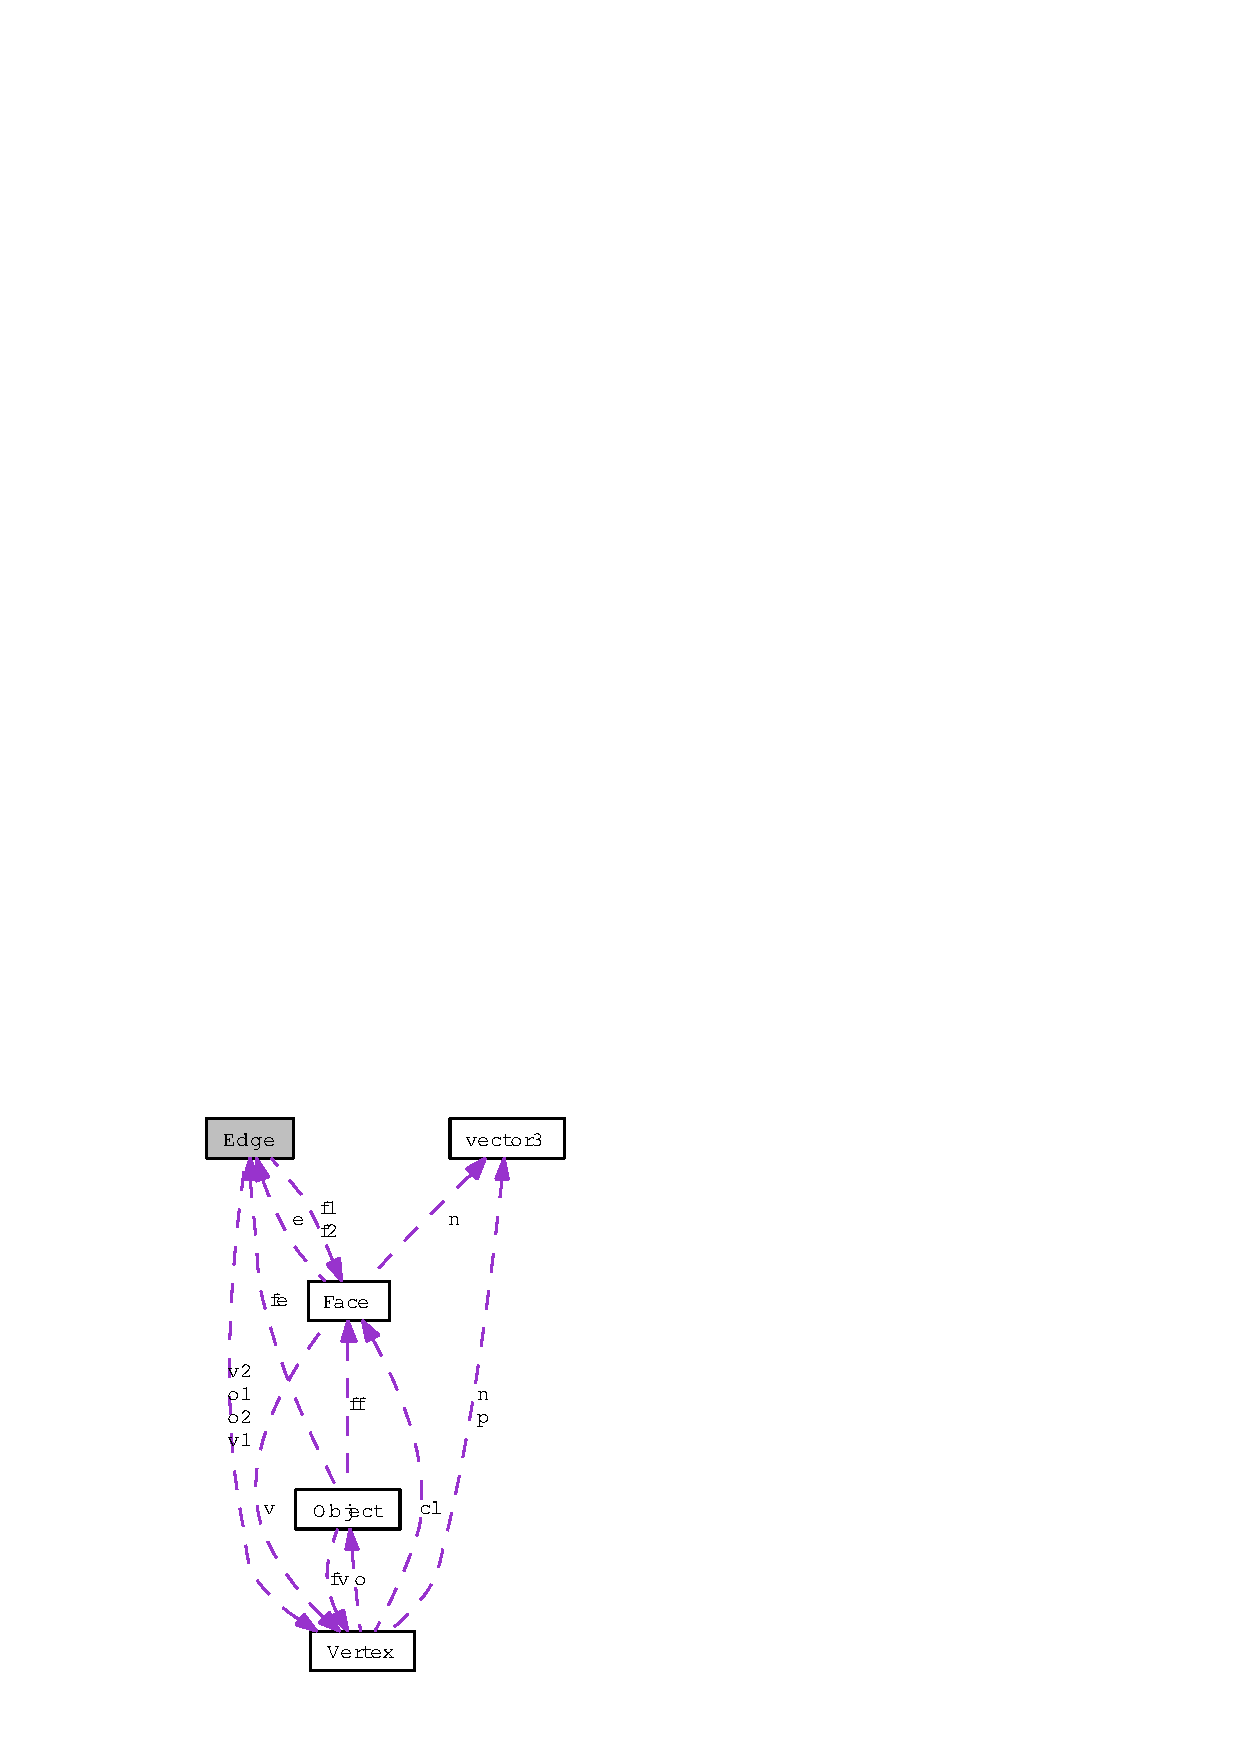
\includegraphics[width=139pt]{classEdge__coll__graph}
\end{center}
\end{figure}
\subsection*{Public Member Functions}
\begin{CompactItemize}
\item 
{\bf Edge} ({\bf Face} $\ast$const, {\bf Vertex} $\ast$const, {\bf Vertex} $\ast$const, {\bf Vertex} $\ast$const)
\item 
void {\bf print} (std::ostream \&) const
\item 
void {\bf update} ({\bf Face} $\ast$const, {\bf Vertex} $\ast$const)
\item 
double {\bf get\-Angle} (void) const
\item 
double {\bf get\-Curvature\-Length} ({\bf Vertex} const $\ast$const o, {\bf Vertex} const $\ast$const v1, {\bf Vertex} const $\ast$const v2, double const \&edge\_\-length) const
\item 
double {\bf get\-Angle\-Force\-Energy} (int const \&, {\bf vector3} \&, bool) const
\item 
void {\bf get\-Angle\-Re\-Force\-Energy} ({\bf vector3} \&, bool) const
\item 
double {\bf get\-Stretch\-Force\-Energy} ({\bf Vertex} const $\ast$const, {\bf vector3} \&, double const \&, bool) const
\item 
{\bf Face} $\ast$ {\bf get\-Face1} (void) const
\item 
{\bf Face} $\ast$ {\bf get\-Face2} (void) const
\item 
{\bf Vertex} $\ast$const {\bf get\-V1} (void)
\item 
{\bf Vertex} $\ast$const {\bf get\-V2} (void)
\item 
{\bf Vertex} $\ast$const {\bf get\-O1} (void)
\item 
{\bf Vertex} $\ast$const {\bf get\-O2} (void)
\item 
double {\bf get\-Original\-Length} (void) const
\item 
double {\bf get\-Sq\-Length} (void) const
\end{CompactItemize}


\subsection{Constructor \& Destructor Documentation}
\index{Edge@{Edge}!Edge@{Edge}}
\index{Edge@{Edge}!Edge@{Edge}}
\subsubsection{\setlength{\rightskip}{0pt plus 5cm}Edge::Edge ({\bf Face} $\ast$ {\em const}, {\bf Vertex} $\ast$ {\em const}, {\bf Vertex} $\ast$ {\em const}, {\bf Vertex} $\ast$ {\em const})}\label{classEdge_a3ce51e560418d2cf41fc86e110c7098}




\subsection{Member Function Documentation}
\index{Edge@{Edge}!print@{print}}
\index{print@{print}!Edge@{Edge}}
\subsubsection{\setlength{\rightskip}{0pt plus 5cm}void Edge::print (std::ostream \& {\em target}) const}\label{classEdge_04f01bd7699b517bef50597951ffc39e}


Write edge description to specified stream. \begin{Desc}
\item[Parameters:]
\begin{description}
\item[\mbox{$\leftarrow$} {\em target}]Output stream; \end{description}
\end{Desc}
\index{Edge@{Edge}!update@{update}}
\index{update@{update}!Edge@{Edge}}
\subsubsection{\setlength{\rightskip}{0pt plus 5cm}void Edge::update ({\bf Face} $\ast$ const {\em f}, {\bf Vertex} $\ast$ const {\em vc})}\label{classEdge_4b04196965158f48b84ceb5f81b90d29}


Add input \doxyref{Face}{p.}{classFace} pointer to this \doxyref{Edge}{p.}{classEdge}. \begin{Desc}
\item[Parameters:]
\begin{description}
\item[\mbox{$\leftarrow$} {\em f}]\doxyref{Face}{p.}{classFace} pointer. \item[\mbox{$\leftarrow$} {\em vc}]Pointer to vertex of second adjacent face to this edge that is not part of this edge. \end{description}
\end{Desc}
\index{Edge@{Edge}!getAngle@{getAngle}}
\index{getAngle@{getAngle}!Edge@{Edge}}
\subsubsection{\setlength{\rightskip}{0pt plus 5cm}double Edge::get\-Angle (void) const}\label{classEdge_b95226f59225e85233d7541ca5c922c3}


Calculate and return edge angle. \begin{Desc}
\item[Returns:]\doxyref{Edge}{p.}{classEdge} angle in radians. \end{Desc}
\index{Edge@{Edge}!getCurvatureLength@{getCurvatureLength}}
\index{getCurvatureLength@{getCurvatureLength}!Edge@{Edge}}
\subsubsection{\setlength{\rightskip}{0pt plus 5cm}double Edge::get\-Curvature\-Length ({\bf Vertex} const $\ast$const  {\em o}, {\bf Vertex} const $\ast$const  {\em vv1}, {\bf Vertex} const $\ast$const  {\em vv2}, double const \& {\em edge\_\-length}) const}\label{classEdge_15abe9cba7f5ccb5a10c0df8aac0e21c}


Get perpendicular length from outer vertex to edge. \begin{Desc}
\item[Parameters:]
\begin{description}
\item[\mbox{$\leftarrow$} {\em o}]Outer vertex of edge. \item[\mbox{$\leftarrow$} {\em vv1}]One edge vertex. \item[\mbox{$\leftarrow$} {\em vv2}]Other edge vertex. \item[\mbox{$\leftarrow$} {\em edge\_\-length}]\doxyref{Edge}{p.}{classEdge} Length. \end{description}
\end{Desc}
\begin{Desc}
\item[Returns:]Perpendicular distance from outer vertex to edge. \end{Desc}
\index{Edge@{Edge}!getAngleForceEnergy@{getAngleForceEnergy}}
\index{getAngleForceEnergy@{getAngleForceEnergy}!Edge@{Edge}}
\subsubsection{\setlength{\rightskip}{0pt plus 5cm}double Edge::get\-Angle\-Force\-Energy (int const \& {\em o2Is\-Requesting}, {\bf vector3} \& {\em force}, bool {\em compute\_\-force}) const}\label{classEdge_b7123bb698409c2142ea0a3e944cd696}


Calculate and return angle force vector and energy. \begin{Desc}
\item[Parameters:]
\begin{description}
\item[\mbox{$\leftarrow$} {\em o2Is\-Requesting}]If nonzero, calculate force and energy at o2 vertex; otherwise calculate for o1 vertex. \item[\mbox{$\rightarrow$} {\em force}]Cumulative force. \item[\mbox{$\leftarrow$} {\em compute\_\-force}]If true then compute force vector; otherwise compute energy only. \end{description}
\end{Desc}
\begin{Desc}
\item[Returns:]Angle energy. \end{Desc}
\index{Edge@{Edge}!getAngleReForceEnergy@{getAngleReForceEnergy}}
\index{getAngleReForceEnergy@{getAngleReForceEnergy}!Edge@{Edge}}
\subsubsection{\setlength{\rightskip}{0pt plus 5cm}void Edge::get\-Angle\-Re\-Force\-Energy ({\bf vector3} \& {\em force}, bool {\em compute\_\-force}) const}\label{classEdge_2f49596cfaef4ba7bc3a1d46373c0c54}


Calculate and return angle reaction force vector and energy. \begin{Desc}
\item[Parameters:]
\begin{description}
\item[\mbox{$\rightarrow$} {\em force}]Input force plus reaction force. \item[\mbox{$\leftarrow$} {\em compute\_\-force}]If true then compute reaction force vector; otherwise compute energy only. \end{description}
\end{Desc}
\begin{Desc}
\item[Returns:]Reaction energy. \end{Desc}
\index{Edge@{Edge}!getStretchForceEnergy@{getStretchForceEnergy}}
\index{getStretchForceEnergy@{getStretchForceEnergy}!Edge@{Edge}}
\subsubsection{\setlength{\rightskip}{0pt plus 5cm}double Edge::get\-Stretch\-Force\-Energy ({\bf Vertex} const $\ast$ const {\em v}, {\bf vector3} \& {\em force}, double const \& {\em mean}, bool {\em compute\_\-force}) const}\label{classEdge_90ebd7292097fa1af3cdad015774b53e}


Compute and return the force vector and energy due to the stretch of the edge. \begin{Desc}
\item[Parameters:]
\begin{description}
\item[\mbox{$\leftarrow$} {\em v}]\doxyref{Vertex}{p.}{classVertex} of interest. \item[\mbox{$\rightarrow$} {\em force}]Cumulative force. \item[\mbox{$\leftarrow$} {\em compute\_\-force}]If true then compute force vector; otherwise compute energy only. \end{description}
\end{Desc}
\index{Edge@{Edge}!getFace1@{getFace1}}
\index{getFace1@{getFace1}!Edge@{Edge}}
\subsubsection{\setlength{\rightskip}{0pt plus 5cm}{\bf Face}$\ast$ Edge::get\-Face1 (void) const}\label{classEdge_e7bf4c264a6353a73bba53eb4d7ef389}


\index{Edge@{Edge}!getFace2@{getFace2}}
\index{getFace2@{getFace2}!Edge@{Edge}}
\subsubsection{\setlength{\rightskip}{0pt plus 5cm}{\bf Face}$\ast$ Edge::get\-Face2 (void) const}\label{classEdge_c6ad9fcb1a330c7bd8b189977692411b}


\index{Edge@{Edge}!getV1@{getV1}}
\index{getV1@{getV1}!Edge@{Edge}}
\subsubsection{\setlength{\rightskip}{0pt plus 5cm}{\bf Vertex}$\ast$ const Edge::get\-V1 (void)\hspace{0.3cm}{\tt  [inline]}}\label{classEdge_dc5033f02e17f29772eb660405d71084}


Get the first vertex of this edge. \begin{Desc}
\item[Returns:]First vertex of this edge. \end{Desc}
\index{Edge@{Edge}!getV2@{getV2}}
\index{getV2@{getV2}!Edge@{Edge}}
\subsubsection{\setlength{\rightskip}{0pt plus 5cm}{\bf Vertex}$\ast$ const Edge::get\-V2 (void)\hspace{0.3cm}{\tt  [inline]}}\label{classEdge_5b2c363204255d8d162ff08218abdaa8}


Get the second vertex of this edge. \begin{Desc}
\item[Returns:]Second vertex of this edge. \end{Desc}
\index{Edge@{Edge}!getO1@{getO1}}
\index{getO1@{getO1}!Edge@{Edge}}
\subsubsection{\setlength{\rightskip}{0pt plus 5cm}{\bf Vertex}$\ast$ const Edge::get\-O1 (void)\hspace{0.3cm}{\tt  [inline]}}\label{classEdge_444b5c81a8e346316576598d16fa7ae5}


Get the non-edge vertex of first adjacent face. \begin{Desc}
\item[Returns:]Non-edge vertex of first adjacent face. \end{Desc}
\index{Edge@{Edge}!getO2@{getO2}}
\index{getO2@{getO2}!Edge@{Edge}}
\subsubsection{\setlength{\rightskip}{0pt plus 5cm}{\bf Vertex}$\ast$ const Edge::get\-O2 (void)\hspace{0.3cm}{\tt  [inline]}}\label{classEdge_b2939e74ece10eecab68fabb246e0236}


Get the non-edge vertex of second adjacent face. \begin{Desc}
\item[Returns:]Non-edge vertex of second adjacent face. \end{Desc}
\index{Edge@{Edge}!getOriginalLength@{getOriginalLength}}
\index{getOriginalLength@{getOriginalLength}!Edge@{Edge}}
\subsubsection{\setlength{\rightskip}{0pt plus 5cm}double Edge::get\-Original\-Length (void) const\hspace{0.3cm}{\tt  [inline]}}\label{classEdge_6b26a07738c9395583ba19e21ea53d10}


Get edge original length. \begin{Desc}
\item[Returns:]\doxyref{Edge}{p.}{classEdge} original length. \end{Desc}
\index{Edge@{Edge}!getSqLength@{getSqLength}}
\index{getSqLength@{getSqLength}!Edge@{Edge}}
\subsubsection{\setlength{\rightskip}{0pt plus 5cm}double Edge::get\-Sq\-Length (void) const\hspace{0.3cm}{\tt  [inline]}}\label{classEdge_8e0c211b2012c3679aeb757575cebead}


Get current squared length of this edge. \begin{Desc}
\item[Returns:]Current squared length of this edge. \end{Desc}


The documentation for this class was generated from the following files:\begin{CompactItemize}
\item 
{\bf edge.h}\item 
{\bf edge.cc}\end{CompactItemize}

\section{Energy Class Reference}
\label{classEnergy}\index{Energy@{Energy}}
{\tt \#include $<$energy.h$>$}

Collaboration diagram for Energy:\begin{figure}[H]
\begin{center}
\leavevmode
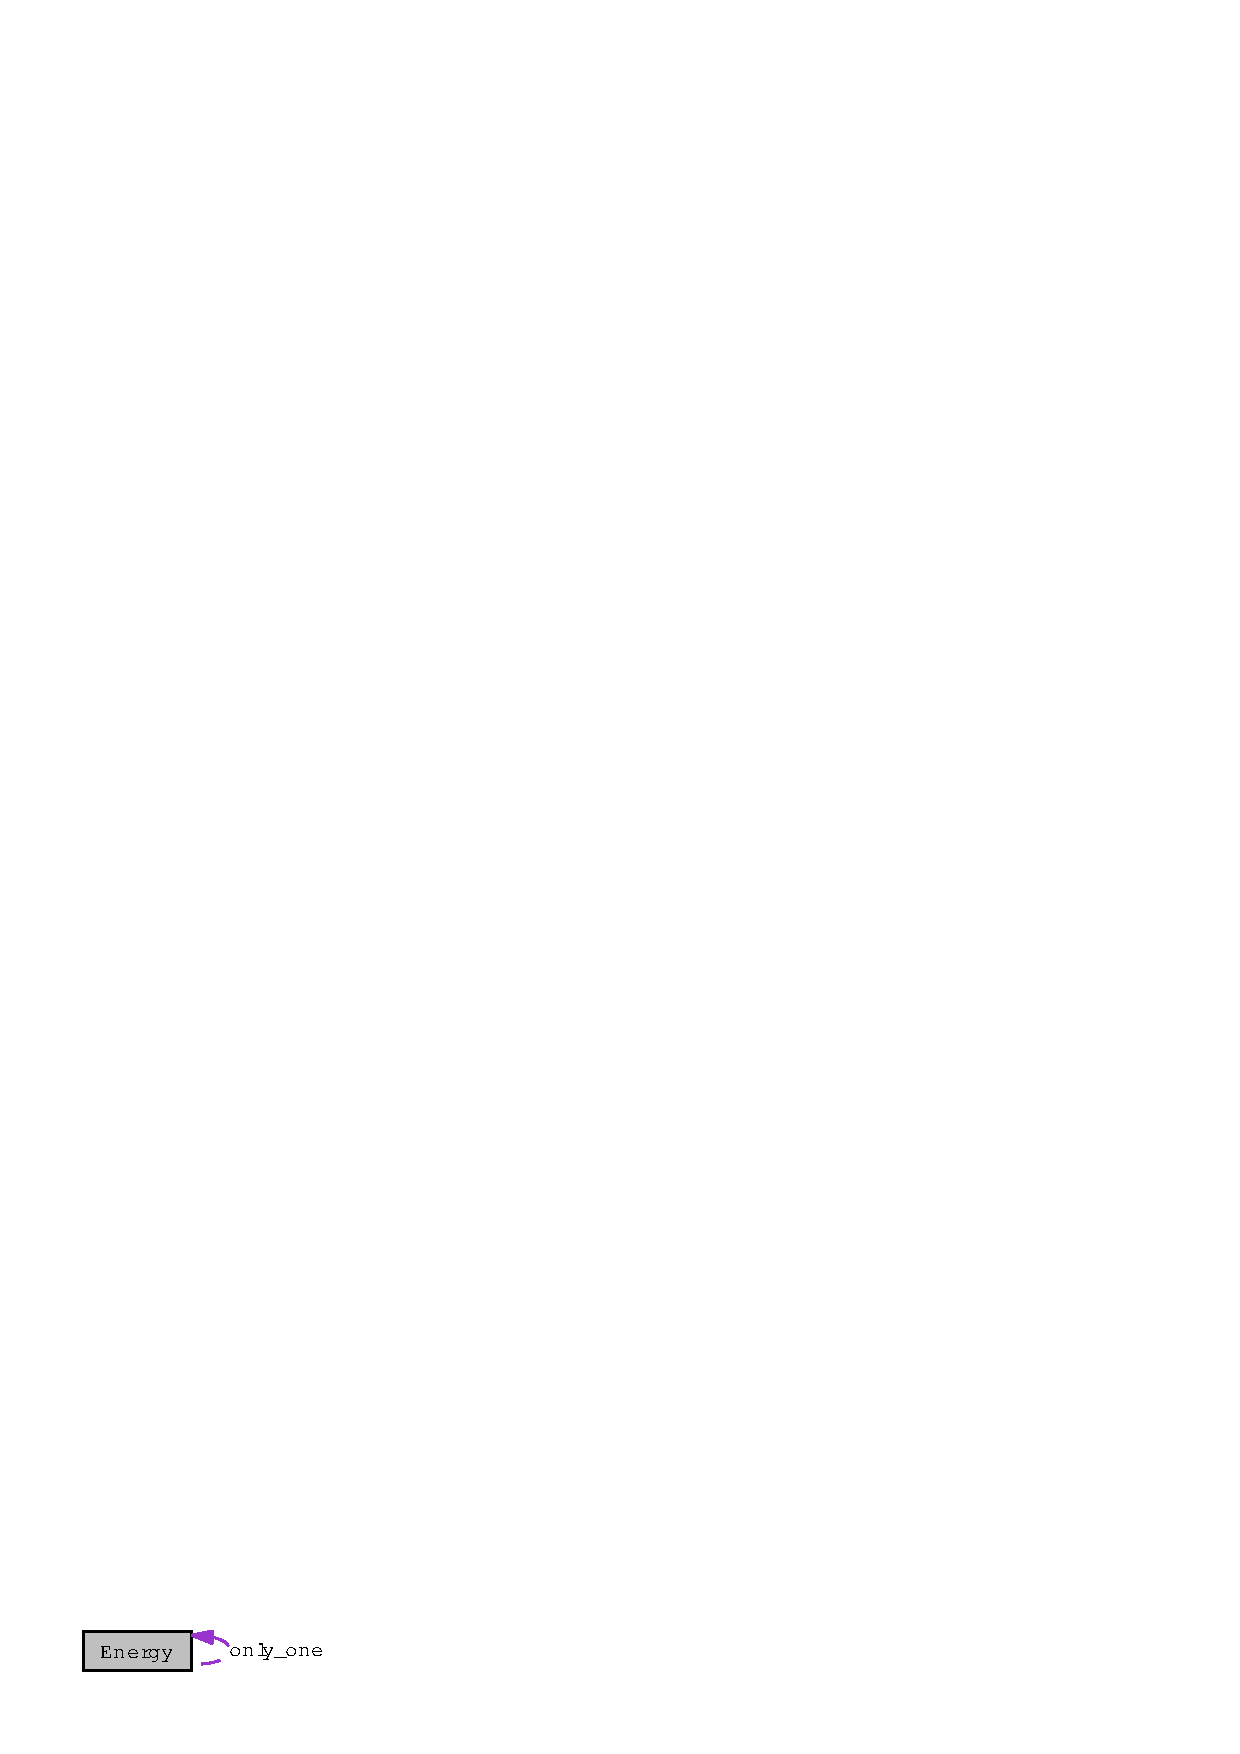
\includegraphics[width=80pt]{classEnergy__coll__graph}
\end{center}
\end{figure}
\subsection*{Public Member Functions}
\begin{CompactItemize}
\item 
void {\bf compute\-Global\-Energy} (void)
\item 
void {\bf write\-Stats} (std::ostream \&)
\end{CompactItemize}
\subsection*{Static Public Member Functions}
\begin{CompactItemize}
\item 
static {\bf Energy} \& {\bf instance} (void)
\end{CompactItemize}


\subsection{Member Function Documentation}
\index{Energy@{Energy}!instance@{instance}}
\index{instance@{instance}!Energy@{Energy}}
\subsubsection{\setlength{\rightskip}{0pt plus 5cm}{\bf Energy} \& Energy::instance (void)\hspace{0.3cm}{\tt  [static]}}\label{classEnergy_0507547be610702ae317b136fd05c31d}


\index{Energy@{Energy}!computeGlobalEnergy@{computeGlobalEnergy}}
\index{computeGlobalEnergy@{computeGlobalEnergy}!Energy@{Energy}}
\subsubsection{\setlength{\rightskip}{0pt plus 5cm}void Energy::compute\-Global\-Energy (void)}\label{classEnergy_fe2e06beeb8f6cadb07bfbd2f8a1d96e}


\index{Energy@{Energy}!writeStats@{writeStats}}
\index{writeStats@{writeStats}!Energy@{Energy}}
\subsubsection{\setlength{\rightskip}{0pt plus 5cm}void Energy::write\-Stats (std::ostream \& {\em target})}\label{classEnergy_818c911e57dd9c7d7be0c8b22f2f1957}


Print total model energy statistics.

\begin{Desc}
\item[Parameters:]
\begin{description}
\item[\mbox{$\leftarrow$} {\em target}]Pre-initialized output stream. \end{description}
\end{Desc}


The documentation for this class was generated from the following files:\begin{CompactItemize}
\item 
{\bf energy.h}\item 
{\bf energy.cc}\end{CompactItemize}

\section{f\_\-hash Struct Reference}
\label{structf__hash}\index{f_hash@{f\_\-hash}}
{\tt \#include $<$meshmorph.h$>$}

\subsection*{Public Member Functions}
\begin{CompactItemize}
\item 
{\bf u4} {\bf operator()} ({\bf Face} $\ast$i) const
\end{CompactItemize}


\subsection{Member Function Documentation}
\index{f_hash@{f\_\-hash}!operator()@{operator()}}
\index{operator()@{operator()}!f_hash@{f\_\-hash}}
\subsubsection{\setlength{\rightskip}{0pt plus 5cm}{\bf u4} f\_\-hash::operator() ({\bf Face} $\ast$ {\em i}) const\hspace{0.3cm}{\tt  [inline]}}\label{structf__hash_2596dc1c7fa5d6012fcb08bd789e5b97}




The documentation for this struct was generated from the following file:\begin{CompactItemize}
\item 
{\bf meshmorph.h}\end{CompactItemize}

\section{Face Class Reference}
\label{classFace}\index{Face@{Face}}
{\tt \#include $<$face.h$>$}

Collaboration diagram for Face:\begin{figure}[H]
\begin{center}
\leavevmode
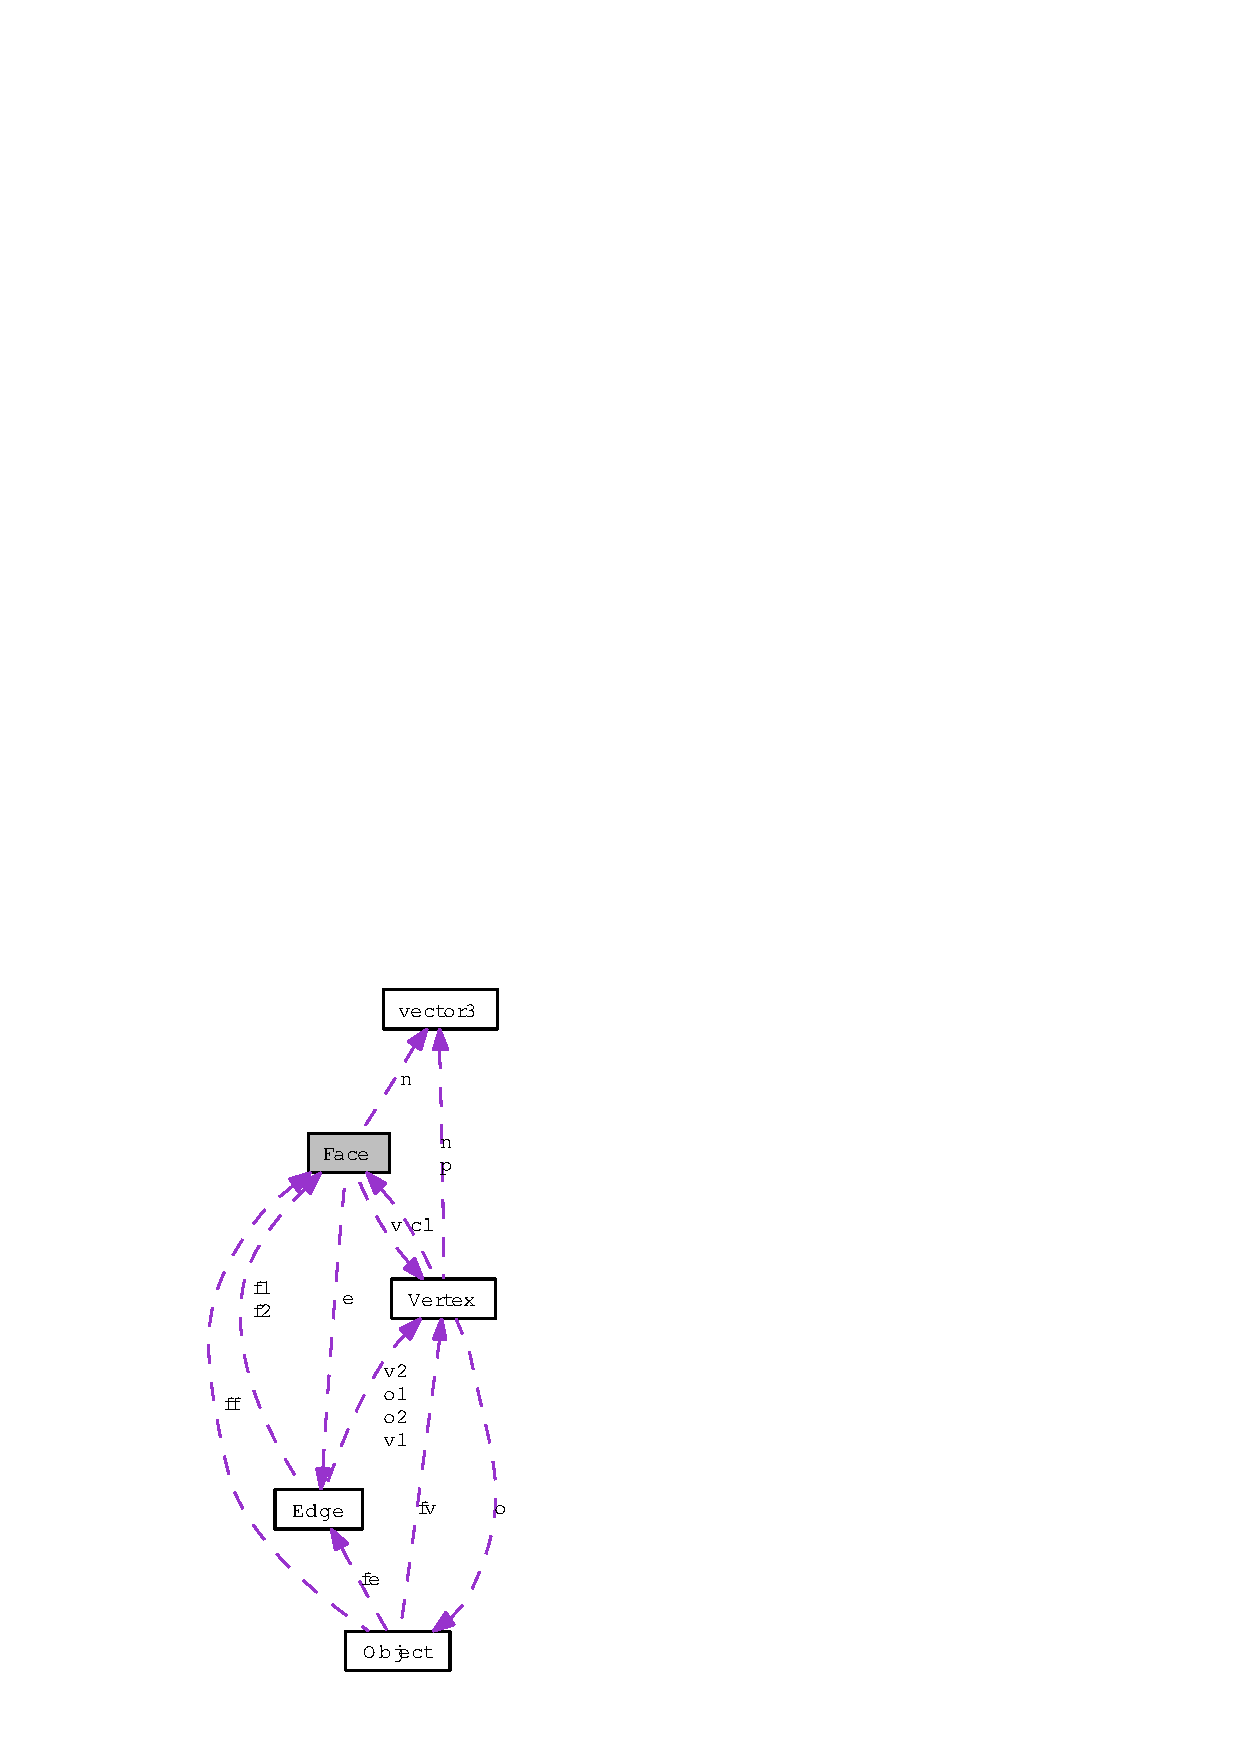
\includegraphics[width=136pt]{classFace__coll__graph}
\end{center}
\end{figure}
\subsection*{Public Member Functions}
\begin{CompactItemize}
\item 
{\bf Face} \& {\bf operator=} ({\bf Face} const \&)
\item 
{\bf Face} (int const \&, int const \&, int const \&, int const \&, {\bf vec\_\-vp} \&)
\item 
{\bf Face} ({\bf Face} const \&)
\item 
bool {\bf is\-Match} (int i, std::string const \&name) const
\item 
void {\bf print} (std::ostream \&) const
\item 
void {\bf print\-CP} (std::ostream \&) const
\item 
void {\bf add\-Edge} ({\bf Edge} $\ast$)
\item 
void {\bf get\-Bounding\-Box} ({\bf hxa7241\_\-graphics::Vector3r} \&lower, {\bf hxa7241\_\-graphics::Vector3r} \&upper) const
\item 
void {\bf get\-Vertex\-Coord} ({\bf vector3} const $\ast$\&, {\bf vector3} const $\ast$\&, {\bf vector3} const $\ast$\&) const
\item 
double {\bf get\-Angle} ({\bf Vertex} const $\ast$const v) const
\item 
double {\bf get\-Angle\-Proxy} ({\bf Vertex} const $\ast$const) const 
\item 
double {\bf get\-Aspect\-Ratio} ({\bf vector3} \&, {\bf Vertex} const $\ast$\&) const
\item 
double {\bf get\-Aspect\-Ratio\-Force\-Energy} ({\bf Vertex} const $\ast$const v, {\bf vector3} \&force, bool compute\_\-force) const 
\item 
void {\bf update\-Normal} (void)
\item 
bool {\bf get\-Flag} (void) const
\item 
void {\bf set\-Flag} (void)
\item 
void {\bf clear\-Flag} (void)
\item 
int {\bf get\-Index} (void) const
\item 
{\bf Edge} $\ast$ {\bf get\-Edge} (int const \&i)
\item 
{\bf Vertex} $\ast$ {\bf get\-Vertex} (int const \&i) const 
\item 
{\bf vector3} const $\ast$ {\bf get\-Normal} (void) const
\item 
double {\bf compute\-Area} (void)
\end{CompactItemize}


\subsection{Constructor \& Destructor Documentation}
\index{Face@{Face}!Face@{Face}}
\index{Face@{Face}!Face@{Face}}
\subsubsection{\setlength{\rightskip}{0pt plus 5cm}Face::Face (int const \& {\em in}, int const \& {\em v1}, int const \& {\em v2}, int const \& {\em v3}, {\bf vec\_\-vp} \& {\em vp})}\label{classFace_ab9295fd3031b7935fa26c8a6260b481}


Creat instance of \doxyref{Face}{p.}{classFace} class. \begin{Desc}
\item[Parameters:]
\begin{description}
\item[\mbox{$\leftarrow$} {\em line}]Single line from input mesh file. \item[\mbox{$\leftarrow$} {\em vp}]Implicit mapping from vertex index to vertex pointer. \end{description}
\end{Desc}
\index{Face@{Face}!Face@{Face}}
\index{Face@{Face}!Face@{Face}}
\subsubsection{\setlength{\rightskip}{0pt plus 5cm}Face::Face ({\bf Face} const \&)}\label{classFace_fb1843b8cdc5aaaa4875ea5550bc3493}




\subsection{Member Function Documentation}
\index{Face@{Face}!operator=@{operator=}}
\index{operator=@{operator=}!Face@{Face}}
\subsubsection{\setlength{\rightskip}{0pt plus 5cm}{\bf Face} \& Face::operator= ({\bf Face} const \&)}\label{classFace_cd891436f2dc7977dbc6a49ce81209c4}


\index{Face@{Face}!isMatch@{isMatch}}
\index{isMatch@{isMatch}!Face@{Face}}
\subsubsection{\setlength{\rightskip}{0pt plus 5cm}bool Face::is\-Match (int {\em i}, std::string const \& {\em name}) const}\label{classFace_7273f790f7b5cb5a4bbcb26d5906b515}


Compare input face index and object name to this face's index and object name.

\begin{Desc}
\item[Parameters:]
\begin{description}
\item[\mbox{$\leftarrow$} {\em i}]Input face index. \item[\mbox{$\leftarrow$} {\em name}]Input face parent object name. \end{description}
\end{Desc}
\begin{Desc}
\item[Returns:]True if indices and names match; false otherwise. \end{Desc}
\index{Face@{Face}!print@{print}}
\index{print@{print}!Face@{Face}}
\subsubsection{\setlength{\rightskip}{0pt plus 5cm}void Face::print (std::ostream \& {\em target}) const}\label{classFace_9eb0f65300ecfc4382a562ce38af6bb7}


Print identifying face information to output stream.

\begin{Desc}
\item[Parameters:]
\begin{description}
\item[\mbox{$\leftarrow$} {\em target}]Pre-initialized output stream. \end{description}
\end{Desc}
\index{Face@{Face}!printCP@{printCP}}
\index{printCP@{printCP}!Face@{Face}}
\subsubsection{\setlength{\rightskip}{0pt plus 5cm}void Face::print\-CP (std::ostream \& {\em target}) const}\label{classFace_2065da4c85bd140413ad08526025e53d}


Print to output stream the position of each vertex of this face in DREa\-MM custom points format.

\begin{Desc}
\item[Parameters:]
\begin{description}
\item[\mbox{$\leftarrow$} {\em target}]Pre-initialized output stream. \end{description}
\end{Desc}
\index{Face@{Face}!addEdge@{addEdge}}
\index{addEdge@{addEdge}!Face@{Face}}
\subsubsection{\setlength{\rightskip}{0pt plus 5cm}void Face::add\-Edge ({\bf Edge} $\ast$ {\em ptr})}\label{classFace_2e1c36f943740d503af6af28400b5a1e}


Add input edge pointer to this face. \begin{Desc}
\item[Parameters:]
\begin{description}
\item[\mbox{$\leftarrow$} {\em ptr}]\doxyref{Edge}{p.}{classEdge} of interest. \end{description}
\end{Desc}
\index{Face@{Face}!getBoundingBox@{getBoundingBox}}
\index{getBoundingBox@{getBoundingBox}!Face@{Face}}
\subsubsection{\setlength{\rightskip}{0pt plus 5cm}void Face::get\-Bounding\-Box ({\bf hxa7241\_\-graphics::Vector3r} \& {\em lower}, {\bf hxa7241\_\-graphics::Vector3r} \& {\em upper}) const}\label{classFace_d72c67513d0cf94806d1d62b4e79033a}


Calculate bounding box of this face. \begin{Desc}
\item[Parameters:]
\begin{description}
\item[\mbox{$\rightarrow$} {\em lower}]Lower corner of bounding box of this face. \item[\mbox{$\rightarrow$} {\em upper}]Upper corner of bounding box of this face. \end{description}
\end{Desc}
\begin{Desc}
\item[Returns:]Limiting extent of face in ith direction. \end{Desc}
\index{Face@{Face}!getVertexCoord@{getVertexCoord}}
\index{getVertexCoord@{getVertexCoord}!Face@{Face}}
\subsubsection{\setlength{\rightskip}{0pt plus 5cm}void Face::get\-Vertex\-Coord ({\bf vector3} const $\ast$\& {\em v0}, {\bf vector3} const $\ast$\& {\em v1}, {\bf vector3} const $\ast$\& {\em v2}) const}\label{classFace_0ff0c505774feeac45b4ed01c6bd4eb8}


Get pointers to face vertex positions. \begin{Desc}
\item[Parameters:]
\begin{description}
\item[\mbox{$\rightarrow$} {\em v0}]Pointer to position of first vertex. \item[\mbox{$\rightarrow$} {\em v1}]Pointer to position of second vertex. \item[\mbox{$\rightarrow$} {\em v2}]Pointer to position of third vertex. \end{description}
\end{Desc}
\index{Face@{Face}!getAngle@{getAngle}}
\index{getAngle@{getAngle}!Face@{Face}}
\subsubsection{\setlength{\rightskip}{0pt plus 5cm}double Face::get\-Angle ({\bf Vertex} const $\ast$const  {\em v}) const}\label{classFace_df9ee7f383efc1a1135c3dd4b5531c37}


\index{Face@{Face}!getAngleProxy@{getAngleProxy}}
\index{getAngleProxy@{getAngleProxy}!Face@{Face}}
\subsubsection{\setlength{\rightskip}{0pt plus 5cm}double Face::get\-Angle\-Proxy ({\bf Vertex} const $\ast$ const {\em vv}) const}\label{classFace_530452fc98f07048050bfca34a5ca469}


Calculate and retun a ratio of face edge lengths that behaves similarly to interior face angle. \begin{Desc}
\item[Parameters:]
\begin{description}
\item[\mbox{$\leftarrow$} {\em vv}]\doxyref{Vertex}{p.}{classVertex} of interest. \end{description}
\end{Desc}
\begin{Desc}
\item[Returns:]Ratio of length of opposite edge to sum of adjacent edges to vertex of interest. \end{Desc}
\index{Face@{Face}!getAspectRatio@{getAspectRatio}}
\index{getAspectRatio@{getAspectRatio}!Face@{Face}}
\subsubsection{\setlength{\rightskip}{0pt plus 5cm}double Face::get\-Aspect\-Ratio ({\bf vector3} \& {\em alt}, {\bf Vertex} const $\ast$\& {\em worst}) const}\label{classFace_a5e6b46c326d300d0e420ce24143be1d}


Calculate and return aspect ratio of this face. \begin{Desc}
\item[Returns:]\doxyref{Face}{p.}{classFace} aspect ratio as longest edge divided by perpendicular triangle height. \end{Desc}
\index{Face@{Face}!getAspectRatioForceEnergy@{getAspectRatioForceEnergy}}
\index{getAspectRatioForceEnergy@{getAspectRatioForceEnergy}!Face@{Face}}
\subsubsection{\setlength{\rightskip}{0pt plus 5cm}double Face::get\-Aspect\-Ratio\-Force\-Energy ({\bf Vertex} const $\ast$const  {\em vv}, {\bf vector3} \& {\em force}, bool {\em compute\_\-force}) const}\label{classFace_56c867ff1a40d2421e715adfab398aa3}


Compute and return the force vector and energy due to the aspect ratio of this face. \begin{Desc}
\item[Parameters:]
\begin{description}
\item[\mbox{$\leftarrow$} {\em v}]\doxyref{Vertex}{p.}{classVertex} of interest. \item[\mbox{$\rightarrow$} {\em force}]Cumulative force. \item[\mbox{$\leftarrow$} {\em compute\_\-force}]If true then compute force vector; otherwise compute energy only. \end{description}
\end{Desc}
\index{Face@{Face}!updateNormal@{updateNormal}}
\index{updateNormal@{updateNormal}!Face@{Face}}
\subsubsection{\setlength{\rightskip}{0pt plus 5cm}void Face::update\-Normal (void)}\label{classFace_fab8bab0149873704b6dc2bad0ceb1ed}


Calculate and record face normal (not guaranteed to be unit vector). \index{Face@{Face}!getFlag@{getFlag}}
\index{getFlag@{getFlag}!Face@{Face}}
\subsubsection{\setlength{\rightskip}{0pt plus 5cm}bool Face::get\-Flag (void) const\hspace{0.3cm}{\tt  [inline]}}\label{classFace_d5a435045d47259da8a745b3b2f3866b}


Get flag of this face. \begin{Desc}
\item[Returns:]Flag value. \end{Desc}
\index{Face@{Face}!setFlag@{setFlag}}
\index{setFlag@{setFlag}!Face@{Face}}
\subsubsection{\setlength{\rightskip}{0pt plus 5cm}void Face::set\-Flag (void)\hspace{0.3cm}{\tt  [inline]}}\label{classFace_f715c08998f029c39f9ab0e70071e91a}


Set flag of this face to true. \index{Face@{Face}!clearFlag@{clearFlag}}
\index{clearFlag@{clearFlag}!Face@{Face}}
\subsubsection{\setlength{\rightskip}{0pt plus 5cm}void Face::clear\-Flag (void)\hspace{0.3cm}{\tt  [inline]}}\label{classFace_950a31e1f2dda519ae3a4023cfdc43b0}


Reset flag of this face to false. \index{Face@{Face}!getIndex@{getIndex}}
\index{getIndex@{getIndex}!Face@{Face}}
\subsubsection{\setlength{\rightskip}{0pt plus 5cm}int Face::get\-Index (void) const\hspace{0.3cm}{\tt  [inline]}}\label{classFace_aa2388588d19089070f914f500f535ad}


Get face index. \begin{Desc}
\item[Returns:]The face index. \end{Desc}
\index{Face@{Face}!getEdge@{getEdge}}
\index{getEdge@{getEdge}!Face@{Face}}
\subsubsection{\setlength{\rightskip}{0pt plus 5cm}{\bf Edge}$\ast$ Face::get\-Edge (int const \& {\em i})\hspace{0.3cm}{\tt  [inline]}}\label{classFace_92fd27b43a9096ca1200dd9351a37cb7}


Get one of edges of this face. \begin{Desc}
\item[Parameters:]
\begin{description}
\item[\mbox{$\leftarrow$} {\em i}]\doxyref{Edge}{p.}{classEdge} of interest. \end{description}
\end{Desc}
\begin{Desc}
\item[Returns:]The ith edge. \end{Desc}
\index{Face@{Face}!getVertex@{getVertex}}
\index{getVertex@{getVertex}!Face@{Face}}
\subsubsection{\setlength{\rightskip}{0pt plus 5cm}{\bf Vertex}$\ast$ Face::get\-Vertex (int const \& {\em i}) const\hspace{0.3cm}{\tt  [inline]}}\label{classFace_139cf7aeff67ced45a85f404607ade56}


Get pointer to face vertex. \begin{Desc}
\item[Parameters:]
\begin{description}
\item[\mbox{$\leftarrow$} {\em i}]Index (0,1,2) of face vertex of interest. \end{description}
\end{Desc}
\begin{Desc}
\item[Returns:]Pointer to vertex of this face. \end{Desc}
\index{Face@{Face}!getNormal@{getNormal}}
\index{getNormal@{getNormal}!Face@{Face}}
\subsubsection{\setlength{\rightskip}{0pt plus 5cm}{\bf vector3} const$\ast$ Face::get\-Normal (void) const\hspace{0.3cm}{\tt  [inline]}}\label{classFace_c4ab940f378cea25d89a9d4398e793ae}


Return face normal (not guaranteed to be unit vector). \begin{Desc}
\item[Returns:]\doxyref{Face}{p.}{classFace} normal. \end{Desc}
\index{Face@{Face}!computeArea@{computeArea}}
\index{computeArea@{computeArea}!Face@{Face}}
\subsubsection{\setlength{\rightskip}{0pt plus 5cm}double Face::compute\-Area (void)\hspace{0.3cm}{\tt  [inline]}}\label{classFace_5f25dd4b4f5c8ec3423f95efa2d110f3}


Calculate face area. \begin{Desc}
\item[Returns:]\doxyref{Face}{p.}{classFace} area. \end{Desc}


The documentation for this class was generated from the following files:\begin{CompactItemize}
\item 
{\bf face.h}\item 
{\bf face.cc}\end{CompactItemize}

\section{face\_\-grp Struct Reference}
\label{structface__grp}\index{face_grp@{face\_\-grp}}
{\tt \#include $<$nice.h$>$}

\subsection*{Public Member Functions}
\begin{CompactItemize}
\item 
{\bf face\_\-grp} (void)
\end{CompactItemize}
\subsection*{Public Attributes}
\begin{CompactItemize}
\item 
{\bf vec\_\-fp} {\bf crossed\_\-faces}
\item 
{\bf vec\_\-fp} {\bf edge\_\-faces}
\end{CompactItemize}


\subsection{Constructor \& Destructor Documentation}
\index{face_grp@{face\_\-grp}!face_grp@{face\_\-grp}}
\index{face_grp@{face\_\-grp}!face_grp@{face\_\-grp}}
\subsubsection{\setlength{\rightskip}{0pt plus 5cm}face\_\-grp::face\_\-grp (void)\hspace{0.3cm}{\tt  [inline]}}\label{structface__grp_c6fb990165cedb5cdff05ae4b712c8d6}




\subsection{Member Data Documentation}
\index{face_grp@{face\_\-grp}!crossed_faces@{crossed\_\-faces}}
\index{crossed_faces@{crossed\_\-faces}!face_grp@{face\_\-grp}}
\subsubsection{\setlength{\rightskip}{0pt plus 5cm}{\bf vec\_\-fp} {\bf face\_\-grp::crossed\_\-faces}}\label{structface__grp_f27d172a5202ccb227b35dfc80808df9}


\index{face_grp@{face\_\-grp}!edge_faces@{edge\_\-faces}}
\index{edge_faces@{edge\_\-faces}!face_grp@{face\_\-grp}}
\subsubsection{\setlength{\rightskip}{0pt plus 5cm}{\bf vec\_\-fp} {\bf face\_\-grp::edge\_\-faces}}\label{structface__grp_24708d04ab4911b8d1f82a28ade452b7}




The documentation for this struct was generated from the following file:\begin{CompactItemize}
\item 
{\bf nice.h}\end{CompactItemize}

\section{Gain\_\-Schedule Class Reference}
\label{classGain__Schedule}\index{Gain_Schedule@{Gain\_\-Schedule}}
{\tt \#include $<$gain\_\-schedule.h$>$}

Collaboration diagram for Gain\_\-Schedule:\begin{figure}[H]
\begin{center}
\leavevmode
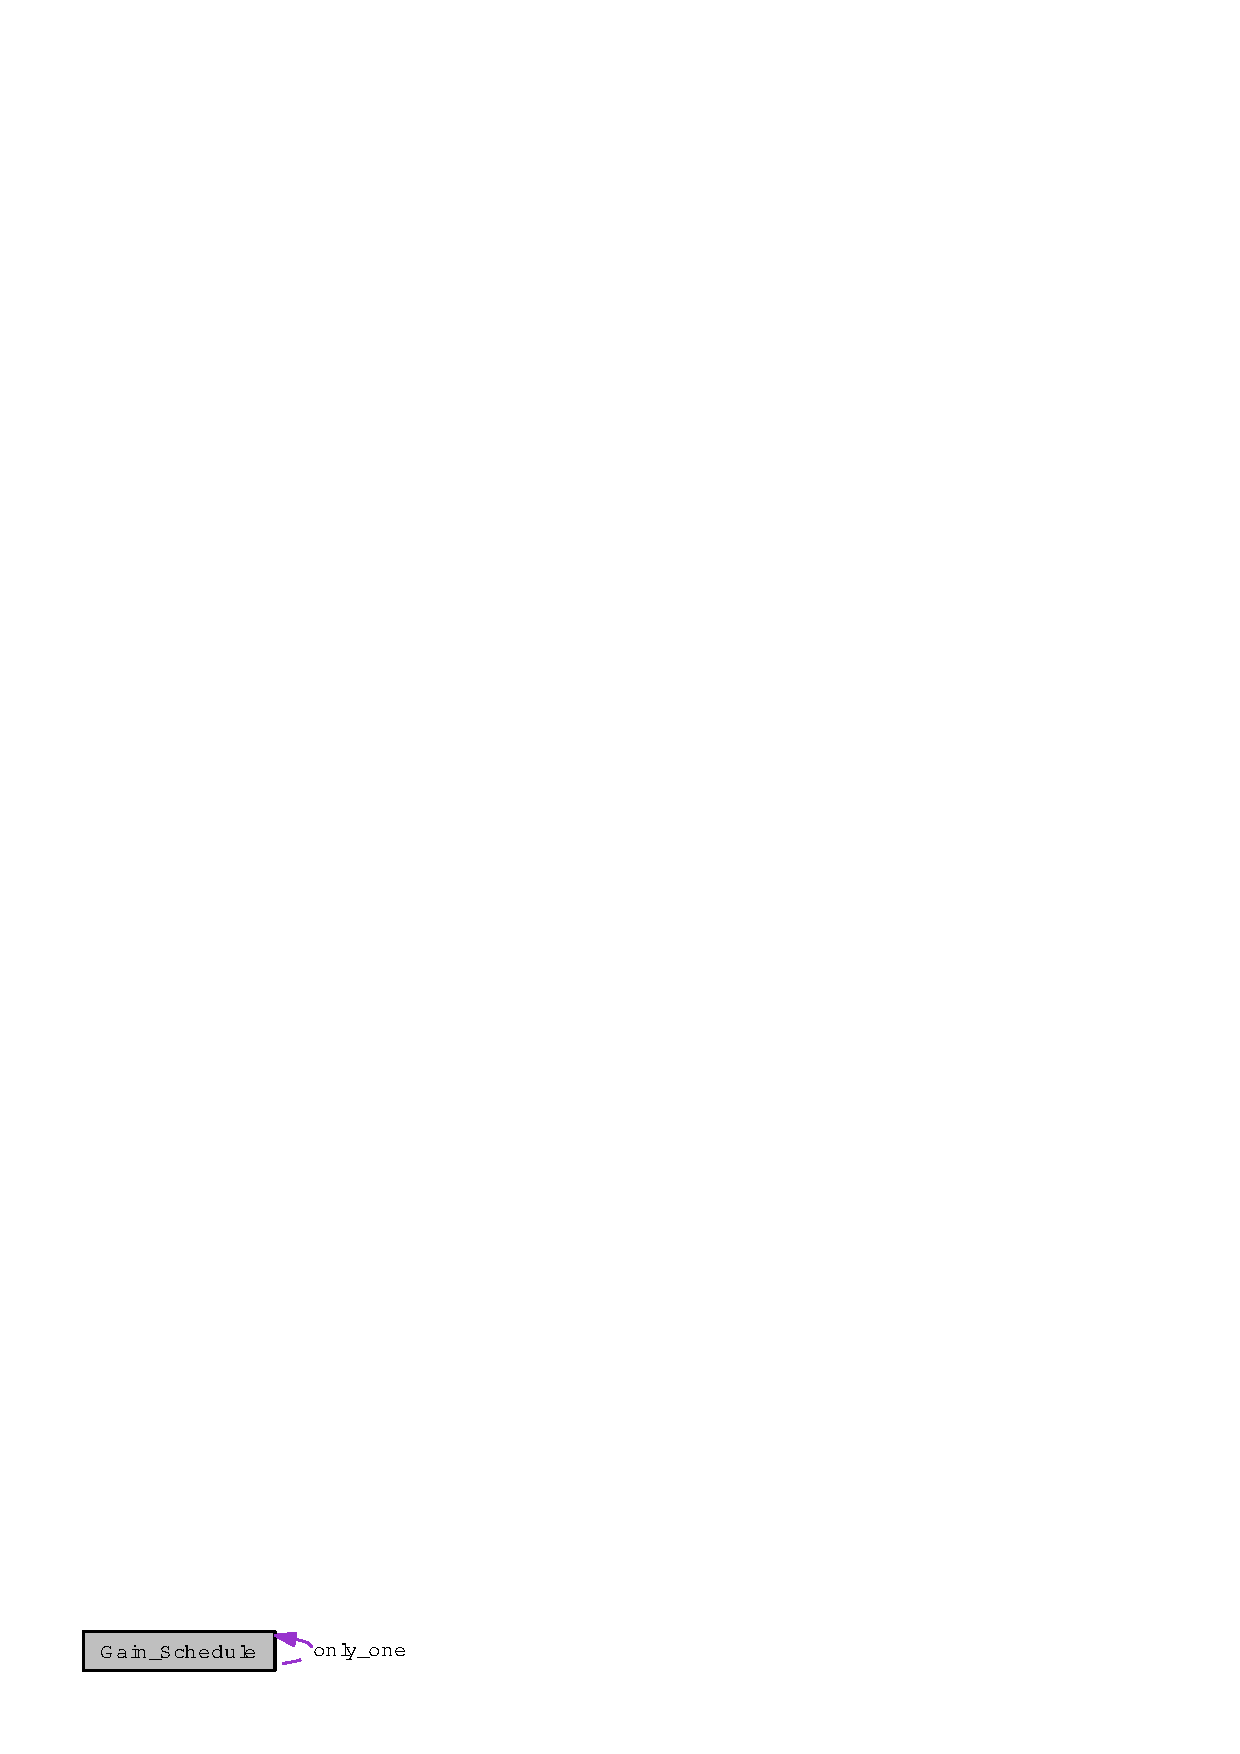
\includegraphics[width=100pt]{classGain__Schedule__coll__graph}
\end{center}
\end{figure}
\subsection*{Public Member Functions}
\begin{CompactItemize}
\item 
void {\bf update\-Max\-Gain} (void)
\item 
double {\bf get\-Max\-Gain} (void) const
\item 
double {\bf get\-Gain} (void) const
\item 
void {\bf reset\-Gain} (void)
\item 
void {\bf halve\-Gain} (void)
\end{CompactItemize}
\subsection*{Static Public Member Functions}
\begin{CompactItemize}
\item 
static {\bf Gain\_\-Schedule} \& {\bf instance} (void)
\end{CompactItemize}


\subsection{Member Function Documentation}
\index{Gain_Schedule@{Gain\_\-Schedule}!instance@{instance}}
\index{instance@{instance}!Gain_Schedule@{Gain\_\-Schedule}}
\subsubsection{\setlength{\rightskip}{0pt plus 5cm}{\bf Gain\_\-Schedule} \& Gain\_\-Schedule::instance (void)\hspace{0.3cm}{\tt  [static]}}\label{classGain__Schedule_e9eeedf767171cf65a3fa1ce7728a48d}


\index{Gain_Schedule@{Gain\_\-Schedule}!updateMaxGain@{updateMaxGain}}
\index{updateMaxGain@{updateMaxGain}!Gain_Schedule@{Gain\_\-Schedule}}
\subsubsection{\setlength{\rightskip}{0pt plus 5cm}void Gain\_\-Schedule::update\-Max\-Gain (void)}\label{classGain__Schedule_6cf994aea246dbfa7c0161a2ea85e8b7}


Update the maximum allowed value of gain and enforce limit. \index{Gain_Schedule@{Gain\_\-Schedule}!getMaxGain@{getMaxGain}}
\index{getMaxGain@{getMaxGain}!Gain_Schedule@{Gain\_\-Schedule}}
\subsubsection{\setlength{\rightskip}{0pt plus 5cm}double Gain\_\-Schedule::get\-Max\-Gain (void) const\hspace{0.3cm}{\tt  [inline]}}\label{classGain__Schedule_a48a7da15dfca933eaf64ff05effb27c}


Get max gain. \begin{Desc}
\item[Returns:]Maximum gain. \end{Desc}
\index{Gain_Schedule@{Gain\_\-Schedule}!getGain@{getGain}}
\index{getGain@{getGain}!Gain_Schedule@{Gain\_\-Schedule}}
\subsubsection{\setlength{\rightskip}{0pt plus 5cm}double Gain\_\-Schedule::get\-Gain (void) const\hspace{0.3cm}{\tt  [inline]}}\label{classGain__Schedule_c39682e959e22b2ce1a701aa11ab40ad}


Get gain. \begin{Desc}
\item[Returns:]Gain. \end{Desc}
\index{Gain_Schedule@{Gain\_\-Schedule}!resetGain@{resetGain}}
\index{resetGain@{resetGain}!Gain_Schedule@{Gain\_\-Schedule}}
\subsubsection{\setlength{\rightskip}{0pt plus 5cm}void Gain\_\-Schedule::reset\-Gain (void)\hspace{0.3cm}{\tt  [inline]}}\label{classGain__Schedule_75dcb2056c045ddaf16f3e72db0696ca}


Reset gain to reference value. /$\ast$$\ast$ Reset gain to max value. \index{Gain_Schedule@{Gain\_\-Schedule}!halveGain@{halveGain}}
\index{halveGain@{halveGain}!Gain_Schedule@{Gain\_\-Schedule}}
\subsubsection{\setlength{\rightskip}{0pt plus 5cm}void Gain\_\-Schedule::halve\-Gain (void)\hspace{0.3cm}{\tt  [inline]}}\label{classGain__Schedule_5fc79542643bd357116aea69735a1ac1}


Reduce gain by 50\%. 

The documentation for this class was generated from the following files:\begin{CompactItemize}
\item 
{\bf gain\_\-schedule.h}\item 
{\bf gain\_\-schedule.cc}\end{CompactItemize}

\section{Grid Struct Reference}
\label{structGrid}\index{Grid@{Grid}}
{\tt \#include $<$grid.h$>$}

Collaboration diagram for Grid:\begin{figure}[H]
\begin{center}
\leavevmode
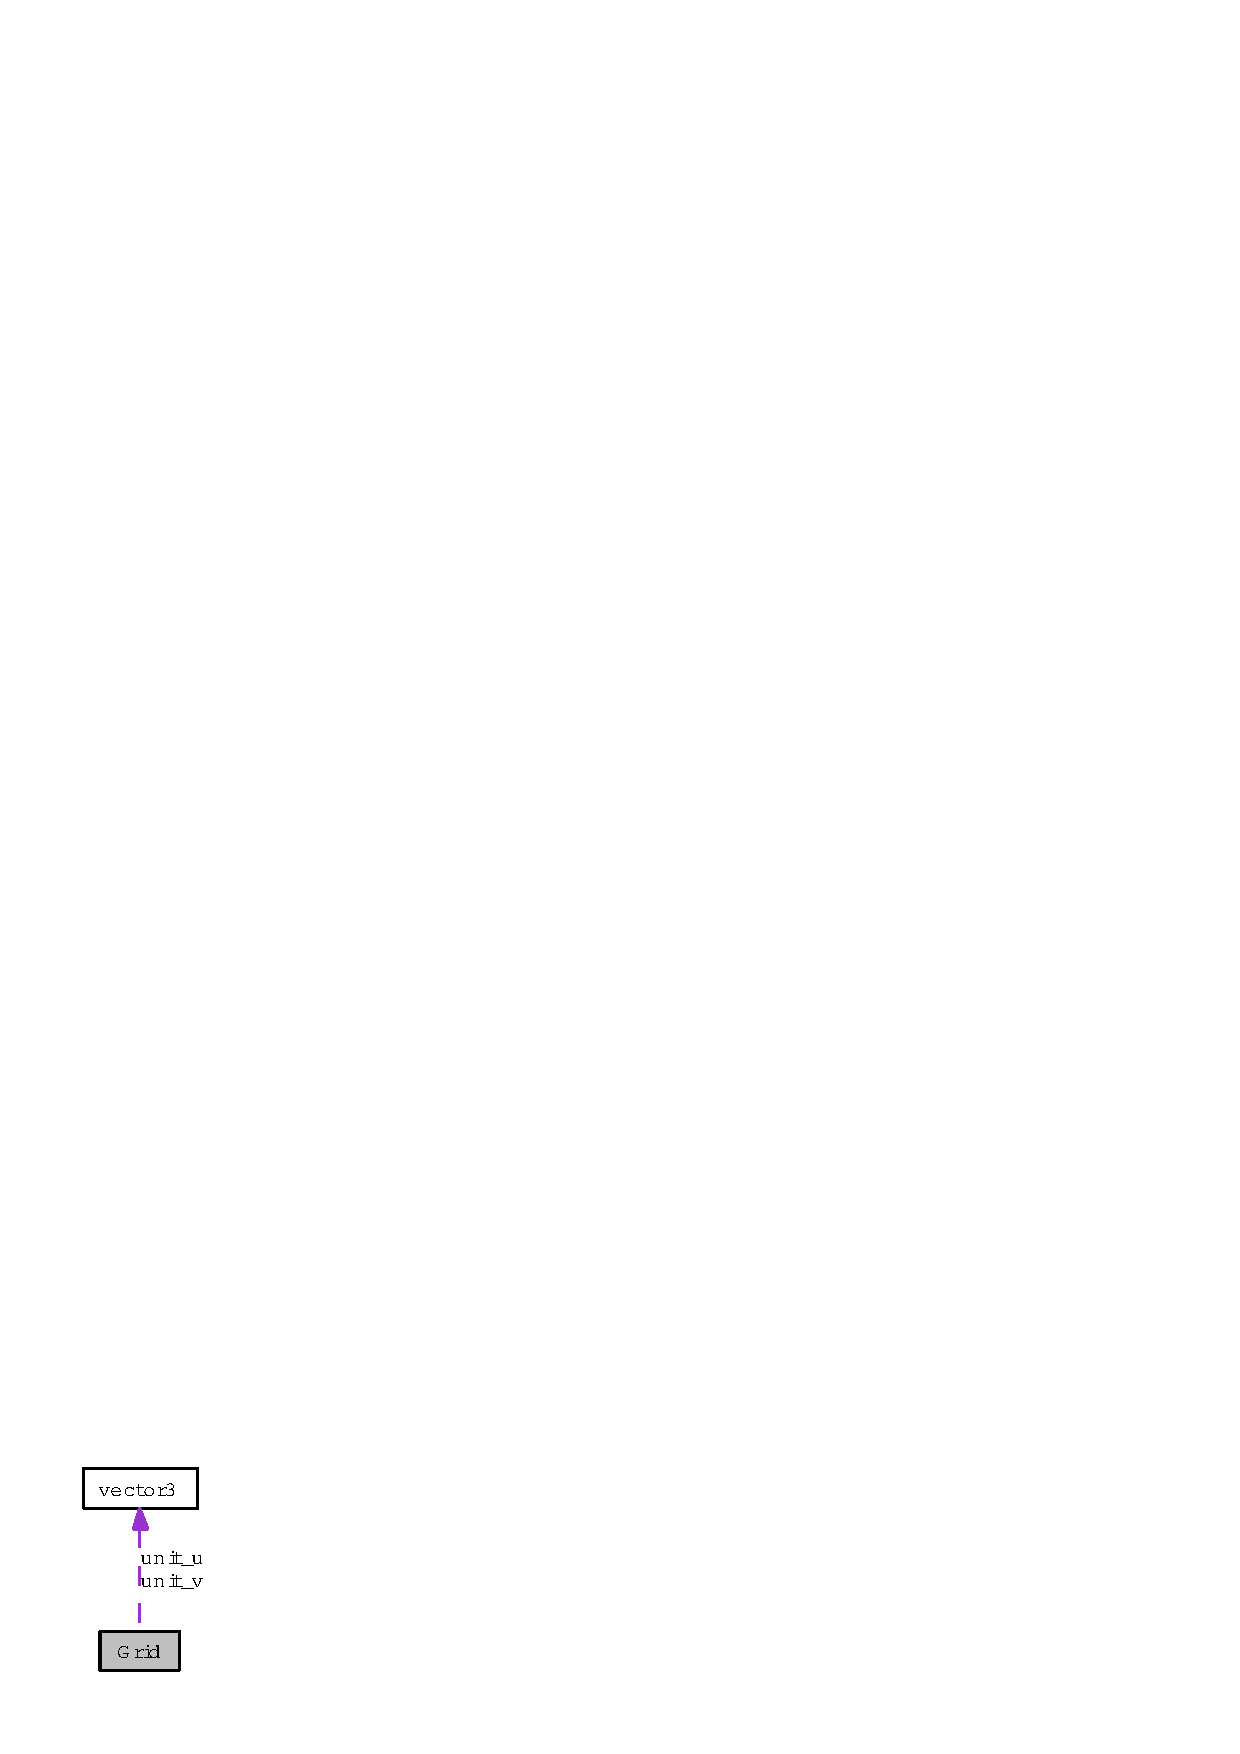
\includegraphics[width=51pt]{structGrid__coll__graph}
\end{center}
\end{figure}
\subsection*{Public Member Functions}
\begin{CompactItemize}
\item 
{\bf Grid} ({\bf Face} $\ast$)
\item 
void {\bf compute\-Barycenter} ({\bf vector3} \&, int, int, {\bf Face} $\ast$)
\end{CompactItemize}
\subsection*{Public Attributes}
\begin{CompactItemize}
\item 
{\bf vector3} {\bf unit\_\-u}
\item 
{\bf vector3} {\bf unit\_\-v}
\item 
double {\bf uv\_\-vert1\_\-u}
\item 
double {\bf uv\_\-vert2} [2]
\end{CompactItemize}


\subsection{Constructor \& Destructor Documentation}
\index{Grid@{Grid}!Grid@{Grid}}
\index{Grid@{Grid}!Grid@{Grid}}
\subsubsection{\setlength{\rightskip}{0pt plus 5cm}Grid::Grid ({\bf Face} $\ast$ {\em f})}\label{structGrid_84af02c866fa15ccc742ce92be1d3add}


Create instance of \doxyref{Grid}{p.}{structGrid}. \begin{Desc}
\item[Parameters:]
\begin{description}
\item[\mbox{$\leftarrow$} {\em f}]\doxyref{Face}{p.}{classFace} of interes. \end{description}
\end{Desc}


\subsection{Member Function Documentation}
\index{Grid@{Grid}!computeBarycenter@{computeBarycenter}}
\index{computeBarycenter@{computeBarycenter}!Grid@{Grid}}
\subsubsection{\setlength{\rightskip}{0pt plus 5cm}void Grid::compute\-Barycenter ({\bf vector3} \& {\em p}, int {\em index}, int {\em n}, {\bf Face} $\ast$ {\em f})}\label{structGrid_4bec6611a861dd9f6f421277dba468b6}


Compute barycenter of face tile. \begin{Desc}
\item[Parameters:]
\begin{description}
\item[\mbox{$\rightarrow$} {\em p}]Barycenter of face tile. \item[\mbox{$\leftarrow$} {\em index}]Index of face tile. \item[\mbox{$\leftarrow$} {\em n}]Not sure what this is. \item[\mbox{$\leftarrow$} {\em f}]\doxyref{Face}{p.}{classFace} of interes. \end{description}
\end{Desc}


\subsection{Member Data Documentation}
\index{Grid@{Grid}!unit_u@{unit\_\-u}}
\index{unit_u@{unit\_\-u}!Grid@{Grid}}
\subsubsection{\setlength{\rightskip}{0pt plus 5cm}{\bf vector3} {\bf Grid::unit\_\-u}}\label{structGrid_4b1f1e9f12cdde6494df39eec543c4b4}


\index{Grid@{Grid}!unit_v@{unit\_\-v}}
\index{unit_v@{unit\_\-v}!Grid@{Grid}}
\subsubsection{\setlength{\rightskip}{0pt plus 5cm}{\bf vector3} {\bf Grid::unit\_\-v}}\label{structGrid_b9d3eedb8715609e39b3681112bd8060}


\index{Grid@{Grid}!uv_vert1_u@{uv\_\-vert1\_\-u}}
\index{uv_vert1_u@{uv\_\-vert1\_\-u}!Grid@{Grid}}
\subsubsection{\setlength{\rightskip}{0pt plus 5cm}double {\bf Grid::uv\_\-vert1\_\-u}}\label{structGrid_a29a486f9d214661cf021226bed94857}


\index{Grid@{Grid}!uv_vert2@{uv\_\-vert2}}
\index{uv_vert2@{uv\_\-vert2}!Grid@{Grid}}
\subsubsection{\setlength{\rightskip}{0pt plus 5cm}double {\bf Grid::uv\_\-vert2}[2]}\label{structGrid_b6b9e0a31025f80a13b01d655aa0abed}




The documentation for this struct was generated from the following files:\begin{CompactItemize}
\item 
{\bf grid.h}\item 
{\bf grid.cc}\end{CompactItemize}

\section{Intersecting\_\-Faces Class Reference}
\label{classIntersecting__Faces}\index{Intersecting_Faces@{Intersecting\_\-Faces}}
{\tt \#include $<$intersecting\_\-faces.h$>$}

Collaboration diagram for Intersecting\_\-Faces:\begin{figure}[H]
\begin{center}
\leavevmode
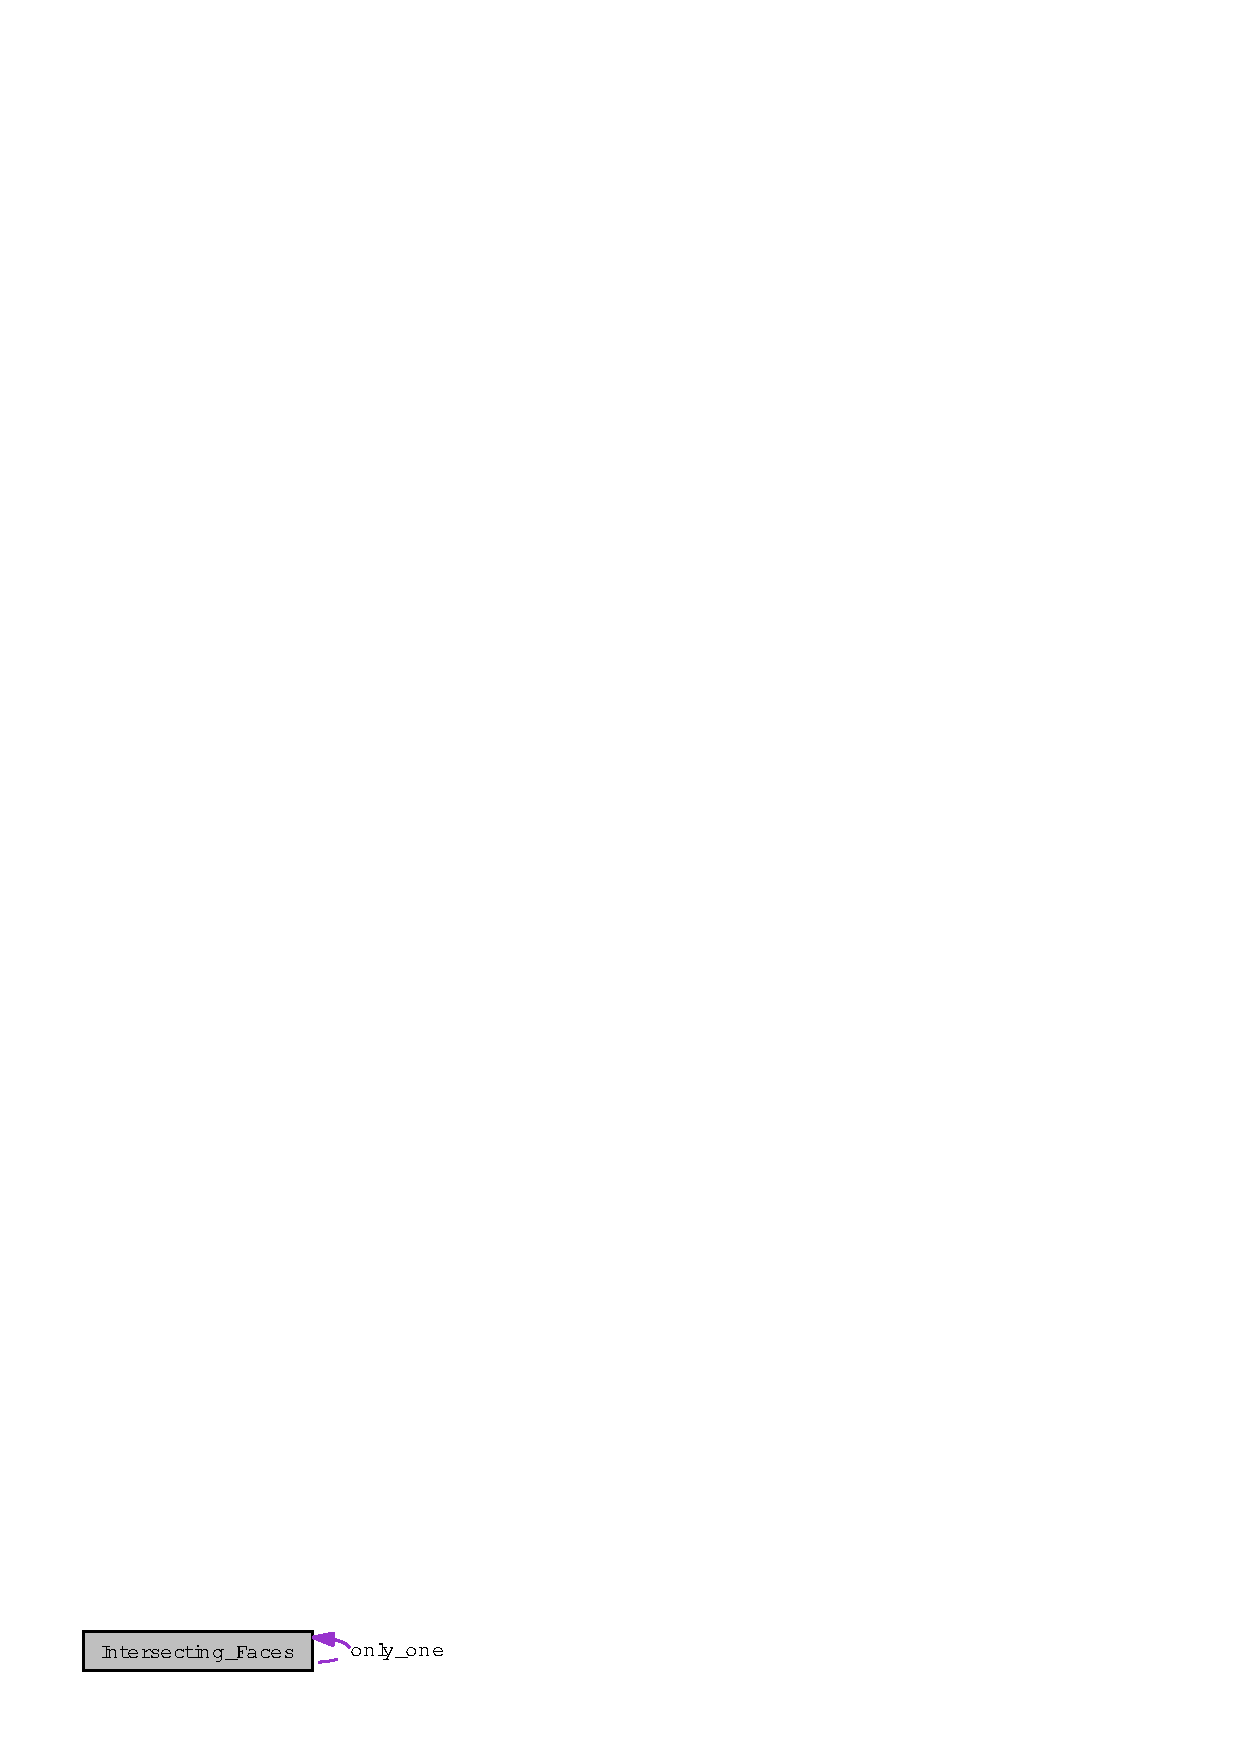
\includegraphics[width=109pt]{classIntersecting__Faces__coll__graph}
\end{center}
\end{figure}
\subsection*{Public Member Functions}
\begin{CompactItemize}
\item 
{\bf vec\_\-fp} $\ast$ {\bf get\-Intersecting\-Faces\-RHS} ({\bf Face} const $\ast$const)
\item 
int {\bf get\-Num\-Unique\-Verts} ({\bf Face} const $\ast$const, {\bf Face} const $\ast$const, int $\ast$const) const
\item 
int {\bf get\-Count\-Of\-Int\-Faces} (bool)
\item 
bool {\bf check\-Face\-Edge\-Int} ({\bf Face} const $\ast$const, {\bf Face} const $\ast$const) const
\item 
bool {\bf check\-Edge\-Edge\-Intersection} ({\bf Face} const $\ast$const, {\bf Face} const $\ast$const) const
\item 
bool {\bf faces\-Parallel} ({\bf Face} const $\ast$const, {\bf Face} const $\ast$const) const
\item 
bool {\bf faces\-Coplanar} ({\bf Face} const $\ast$const, {\bf Face} const $\ast$const) const
\item 
bool {\bf face\-Intersects\-Face} ({\bf Face} const $\ast$const haystack, {\bf Face} const $\ast$const needle)
\item 
bool {\bf face\-Is\-Intersected\-RHS} ({\bf Face} const $\ast$const) const
\item 
bool {\bf find\-And\-Record\-New\-Face\-Int} ({\bf Face} $\ast$const)
\item 
bool {\bf vert\-Adj\-Faces\-Have\-New\-Int} ({\bf Vertex} const $\ast$const)
\item 
bool {\bf check\-Face\-Face\-Ints} ({\bf Face} const $\ast$const, {\bf Face} const $\ast$const) const
\item 
bool {\bf detect\-New\-Face\-Ints} ({\bf Face} $\ast$const)
\item 
void {\bf get\-Nice\-Set} ({\bf v\_\-set} \&, {\bf hashset\_\-v} \&)
\item 
{\bf hashset\_\-v} {\bf get\-Nice\-Check\-Set} ({\bf Vertex} const $\ast$const)
\item 
void {\bf add\-Face\-To\-Face} ({\bf Face} $\ast$const, {\bf Face} const $\ast$const)
\item 
void {\bf remove\-Old\-Intersections} ({\bf Vertex} const $\ast$const, {\bf hashset\_\-v} \&)
\item 
void {\bf update\-New\-Intersections} ({\bf Vertex} const $\ast$const, {\bf hashset\_\-v} \&)
\item 
void {\bf find\-All\-Face\-Intersections} (void)
\item 
void {\bf set\-Face\-Not\-Intersected\-LHS} ({\bf Face} const $\ast$const)
\item 
void {\bf remove\-Face\-From\-Face\-Int} ({\bf Face} $\ast$const haystack, {\bf Face} const $\ast$const needle)
\item 
void {\bf get\-Face\-Intersection\-Force} ({\bf Face} $\ast$const f, {\bf vector3} \&total\_\-force)
\item 
void {\bf get\-Face\-Face\-Int\-Force} ({\bf Face} $\ast$const lhs, {\bf Face} $\ast$const rhs, {\bf vector3} \&)
\item 
bool {\bf face\-Is\-Intersected\-LHS} ({\bf Face} const $\ast$const face) const
\item 
{\bf htff\_\-cit} {\bf begin} (void)
\item 
{\bf htff\_\-cit} {\bf end} (void)
\end{CompactItemize}
\subsection*{Static Public Member Functions}
\begin{CompactItemize}
\item 
static {\bf Intersecting\_\-Faces} \& {\bf instance} (void)
\end{CompactItemize}


\subsection{Member Function Documentation}
\index{Intersecting_Faces@{Intersecting\_\-Faces}!instance@{instance}}
\index{instance@{instance}!Intersecting_Faces@{Intersecting\_\-Faces}}
\subsubsection{\setlength{\rightskip}{0pt plus 5cm}{\bf Intersecting\_\-Faces} \& Intersecting\_\-Faces::instance (void)\hspace{0.3cm}{\tt  [static]}}\label{classIntersecting__Faces_8ccec8bb3cfc50e4ad98ff13c1f8ec8f}


\index{Intersecting_Faces@{Intersecting\_\-Faces}!getIntersectingFacesRHS@{getIntersectingFacesRHS}}
\index{getIntersectingFacesRHS@{getIntersectingFacesRHS}!Intersecting_Faces@{Intersecting\_\-Faces}}
\subsubsection{\setlength{\rightskip}{0pt plus 5cm}{\bf vec\_\-fp} $\ast$ Intersecting\_\-Faces::get\-Intersecting\-Faces\-RHS ({\bf Face} const $\ast$ const {\em face})}\label{classIntersecting__Faces_293abeb5536fd3d69c82f44775d28396}


Return the stored collection of faces that intersect the input \doxyref{Face}{p.}{classFace}. \begin{Desc}
\item[Parameters:]
\begin{description}
\item[\mbox{$\leftarrow$} {\em face}]Intersected face of interest. \end{description}
\end{Desc}
\begin{Desc}
\item[Returns:]Pointer to collection of interecting faces of input face. \end{Desc}
\index{Intersecting_Faces@{Intersecting\_\-Faces}!getNumUniqueVerts@{getNumUniqueVerts}}
\index{getNumUniqueVerts@{getNumUniqueVerts}!Intersecting_Faces@{Intersecting\_\-Faces}}
\subsubsection{\setlength{\rightskip}{0pt plus 5cm}int Intersecting\_\-Faces::get\-Num\-Unique\-Verts ({\bf Face} const $\ast$ const {\em cf}, {\bf Face} const $\ast$ const {\em of}, int $\ast$ const {\em single\_\-shared}) const}\label{classIntersecting__Faces_d812af27b814d33dc7a59de051302a1b}


Count number of unique vertices for pair of faces, and, if exactly one shared vertex, then identify shared vertex in each face.

\begin{Desc}
\item[Parameters:]
\begin{description}
\item[\mbox{$\leftarrow$} {\em cf}]The current face. \item[\mbox{$\leftarrow$} {\em of}]The other face. \item[\mbox{$\rightarrow$} {\em single\_\-shared}]If exactly one shared vertex, then save it's identity in each face. \end{description}
\end{Desc}
\begin{Desc}
\item[Returns:]Number of unique vertices for pair of faces. \end{Desc}
\index{Intersecting_Faces@{Intersecting\_\-Faces}!getCountOfIntFaces@{getCountOfIntFaces}}
\index{getCountOfIntFaces@{getCountOfIntFaces}!Intersecting_Faces@{Intersecting\_\-Faces}}
\subsubsection{\setlength{\rightskip}{0pt plus 5cm}int Intersecting\_\-Faces::get\-Count\-Of\-Int\-Faces (bool {\em detect\_\-self})}\label{classIntersecting__Faces_a1a58bcebe21681324ab18ac410383b2}


Calculate and return the number of intersecting face pairs in model or only the number of intersecting pairs from faces of the same object. \begin{Desc}
\item[Parameters:]
\begin{description}
\item[\mbox{$\leftarrow$} {\em detect\_\-self}]If true then only count intersections between faces of the same object. \end{description}
\end{Desc}
\begin{Desc}
\item[Returns:]Count of pairs of intersecting faces. \end{Desc}
\index{Intersecting_Faces@{Intersecting\_\-Faces}!checkFaceEdgeInt@{checkFaceEdgeInt}}
\index{checkFaceEdgeInt@{checkFaceEdgeInt}!Intersecting_Faces@{Intersecting\_\-Faces}}
\subsubsection{\setlength{\rightskip}{0pt plus 5cm}bool Intersecting\_\-Faces::check\-Face\-Edge\-Int ({\bf Face} const $\ast$ {\em const}, {\bf Face} const $\ast$ {\em const}) const}\label{classIntersecting__Faces_afeb4b57fe4b16e5b5af73c300eaf64f}


\index{Intersecting_Faces@{Intersecting\_\-Faces}!checkEdgeEdgeIntersection@{checkEdgeEdgeIntersection}}
\index{checkEdgeEdgeIntersection@{checkEdgeEdgeIntersection}!Intersecting_Faces@{Intersecting\_\-Faces}}
\subsubsection{\setlength{\rightskip}{0pt plus 5cm}bool Intersecting\_\-Faces::check\-Edge\-Edge\-Intersection ({\bf Face} const $\ast$ const {\em cf}, {\bf Face} const $\ast$ const {\em of}) const}\label{classIntersecting__Faces_19dfb2b12487547e5d2322b6f8f2e549}


For a pair of faces, each edge of each face is checked for intersection with an edge of the other face.

\begin{Desc}
\item[Parameters:]
\begin{description}
\item[\mbox{$\leftarrow$} {\em cf}]The current face. \item[\mbox{$\leftarrow$} {\em of}]The other face. \end{description}
\end{Desc}
\begin{Desc}
\item[Returns:]True if faces intersect, otherwise false. \end{Desc}
\index{Intersecting_Faces@{Intersecting\_\-Faces}!facesParallel@{facesParallel}}
\index{facesParallel@{facesParallel}!Intersecting_Faces@{Intersecting\_\-Faces}}
\subsubsection{\setlength{\rightskip}{0pt plus 5cm}bool Intersecting\_\-Faces::faces\-Parallel ({\bf Face} const $\ast$ const {\em cf}, {\bf Face} const $\ast$ const {\em of}) const}\label{classIntersecting__Faces_bdd45262cca89eafcdbe8e2c40560001}


Check if pair of faces are parallel.

\begin{Desc}
\item[Parameters:]
\begin{description}
\item[\mbox{$\leftarrow$} {\em cf}]The current face. \item[\mbox{$\leftarrow$} {\em of}]The other face. \end{description}
\end{Desc}
\begin{Desc}
\item[Returns:]True if faces are parallel, otherwise false. \end{Desc}
\index{Intersecting_Faces@{Intersecting\_\-Faces}!facesCoplanar@{facesCoplanar}}
\index{facesCoplanar@{facesCoplanar}!Intersecting_Faces@{Intersecting\_\-Faces}}
\subsubsection{\setlength{\rightskip}{0pt plus 5cm}bool Intersecting\_\-Faces::faces\-Coplanar ({\bf Face} const $\ast$ {\em const}, {\bf Face} const $\ast$ {\em const}) const}\label{classIntersecting__Faces_8aa976ef7b7f18ba88985889692e42d5}


\index{Intersecting_Faces@{Intersecting\_\-Faces}!faceIntersectsFace@{faceIntersectsFace}}
\index{faceIntersectsFace@{faceIntersectsFace}!Intersecting_Faces@{Intersecting\_\-Faces}}
\subsubsection{\setlength{\rightskip}{0pt plus 5cm}bool Intersecting\_\-Faces::face\-Intersects\-Face ({\bf Face} const $\ast$const {\em lhs}, {\bf Face} const $\ast$const {\em rhs})}\label{classIntersecting__Faces_40b7910a771bb321d66967a738f5501a}


Determine if an intersection between two faces is recorded in class. \begin{Desc}
\item[Parameters:]
\begin{description}
\item[\mbox{$\leftarrow$} {\em lhs}]\doxyref{Face}{p.}{classFace} pointer to use as key of intersecting faces table. \item[\mbox{$\leftarrow$} {\em rhs}]Putative intersecting face of lhs face. \end{description}
\end{Desc}
\begin{Desc}
\item[Returns:]True if rhs is found in collection of intersecting faces for lhs (with note to the directionality of check); otherwise false. \end{Desc}
\index{Intersecting_Faces@{Intersecting\_\-Faces}!faceIsIntersectedRHS@{faceIsIntersectedRHS}}
\index{faceIsIntersectedRHS@{faceIsIntersectedRHS}!Intersecting_Faces@{Intersecting\_\-Faces}}
\subsubsection{\setlength{\rightskip}{0pt plus 5cm}bool Intersecting\_\-Faces::face\-Is\-Intersected\-RHS ({\bf Face} const $\ast$ const {\em face}) const}\label{classIntersecting__Faces_533016761a360de5de059ce179acd1a1}


Strongly determine if input face is recorded in class as being intersected. \begin{Desc}
\item[Parameters:]
\begin{description}
\item[\mbox{$\leftarrow$} {\em face}]\doxyref{Face}{p.}{classFace} of interest. \end{description}
\end{Desc}
\begin{Desc}
\item[Returns:]True if face is used as key in intersecting faces container and has faces stored as intersecting.; otherwise false. \end{Desc}
\index{Intersecting_Faces@{Intersecting\_\-Faces}!findAndRecordNewFaceInt@{findAndRecordNewFaceInt}}
\index{findAndRecordNewFaceInt@{findAndRecordNewFaceInt}!Intersecting_Faces@{Intersecting\_\-Faces}}
\subsubsection{\setlength{\rightskip}{0pt plus 5cm}bool Intersecting\_\-Faces::find\-And\-Record\-New\-Face\-Int ({\bf Face} $\ast$ const {\em face})}\label{classIntersecting__Faces_c1bb38e2d09c62762bfa566bdb21bdf5}


Find and record all intersecting faces of input face.

\begin{Desc}
\item[Parameters:]
\begin{description}
\item[\mbox{$\leftarrow$} {\em face}]\doxyref{Face}{p.}{classFace} of interest. \end{description}
\end{Desc}
\begin{Desc}
\item[Returns:]True if current face is intersected, false otherwise. \end{Desc}
\index{Intersecting_Faces@{Intersecting\_\-Faces}!vertAdjFacesHaveNewInt@{vertAdjFacesHaveNewInt}}
\index{vertAdjFacesHaveNewInt@{vertAdjFacesHaveNewInt}!Intersecting_Faces@{Intersecting\_\-Faces}}
\subsubsection{\setlength{\rightskip}{0pt plus 5cm}bool Intersecting\_\-Faces::vert\-Adj\-Faces\-Have\-New\-Int ({\bf Vertex} const $\ast$ const {\em v})}\label{classIntersecting__Faces_d0b9954e791421bbdbcdc0aa6bc13a88}


Check if any adjacent face of current vertex is intersected.

\begin{Desc}
\item[Parameters:]
\begin{description}
\item[\mbox{$\leftarrow$} {\em v}]The current vertex. \end{description}
\end{Desc}
\begin{Desc}
\item[Returns:]True if any adjacent face of vertex is intersected, false otherwise. \end{Desc}
\index{Intersecting_Faces@{Intersecting\_\-Faces}!checkFaceFaceInts@{checkFaceFaceInts}}
\index{checkFaceFaceInts@{checkFaceFaceInts}!Intersecting_Faces@{Intersecting\_\-Faces}}
\subsubsection{\setlength{\rightskip}{0pt plus 5cm}bool Intersecting\_\-Faces::check\-Face\-Face\-Ints ({\bf Face} const $\ast$ const {\em cf}, {\bf Face} const $\ast$ const {\em of}) const}\label{classIntersecting__Faces_f15a18276918e03d465d56b9b25af3b1}


For a pair of faces, each edge of each face is checked for intersection with other face.

\begin{Desc}
\item[Parameters:]
\begin{description}
\item[\mbox{$\leftarrow$} {\em cf}]The current face. \item[\mbox{$\leftarrow$} {\em of}]The other face. \end{description}
\end{Desc}
\begin{Desc}
\item[Returns:]True if faces intersect, otherwise false. \end{Desc}
\index{Intersecting_Faces@{Intersecting\_\-Faces}!detectNewFaceInts@{detectNewFaceInts}}
\index{detectNewFaceInts@{detectNewFaceInts}!Intersecting_Faces@{Intersecting\_\-Faces}}
\subsubsection{\setlength{\rightskip}{0pt plus 5cm}bool Intersecting\_\-Faces::detect\-New\-Face\-Ints ({\bf Face} $\ast$ const {\em face})}\label{classIntersecting__Faces_95e540a24135003654fa037dbfaa25a0}


Search for new face intersections with input face. \begin{Desc}
\item[Parameters:]
\begin{description}
\item[\mbox{$\leftarrow$} {\em face}]\doxyref{Face}{p.}{classFace} of interest. \end{description}
\end{Desc}
\begin{Desc}
\item[Returns:]True if new face intersections are detected; false otherwise. \end{Desc}
\index{Intersecting_Faces@{Intersecting\_\-Faces}!getNiceSet@{getNiceSet}}
\index{getNiceSet@{getNiceSet}!Intersecting_Faces@{Intersecting\_\-Faces}}
\subsubsection{\setlength{\rightskip}{0pt plus 5cm}void Intersecting\_\-Faces::get\-Nice\-Set ({\bf v\_\-set} \& {\em full\_\-search\_\-faces}, {\bf hashset\_\-v} \& {\em vertices})}\label{classIntersecting__Faces_0a15c1e789d63ebcb8d0d9b8198ecd32}


Check niceness of each collected vertex, and, if niceness changed, then add vertex to set of verticess requiring a full closest point search.

\begin{Desc}
\item[Parameters:]
\begin{description}
\item[\mbox{$\rightarrow$} {\em full\_\-search\_\-faces}]The collection of vertices requiring full search. \item[\mbox{$\leftarrow$} {\em vertices}]Collection of vertices whose niceness may have changed. \end{description}
\end{Desc}
\index{Intersecting_Faces@{Intersecting\_\-Faces}!getNiceCheckSet@{getNiceCheckSet}}
\index{getNiceCheckSet@{getNiceCheckSet}!Intersecting_Faces@{Intersecting\_\-Faces}}
\subsubsection{\setlength{\rightskip}{0pt plus 5cm}{\bf hashset\_\-v} Intersecting\_\-Faces::get\-Nice\-Check\-Set ({\bf Vertex} const $\ast$ const {\em v})}\label{classIntersecting__Faces_540d46017e3f03c2e26052b31e99ded1}


Collect vertices whose niceness may have changed after vertex move due to face intersections.

\begin{Desc}
\item[Parameters:]
\begin{description}
\item[\mbox{$\leftarrow$} {\em v}]The current vertex. \end{description}
\end{Desc}
\begin{Desc}
\item[Returns:]Collection of vertices whose niceness may have changed. \end{Desc}
\index{Intersecting_Faces@{Intersecting\_\-Faces}!addFaceToFace@{addFaceToFace}}
\index{addFaceToFace@{addFaceToFace}!Intersecting_Faces@{Intersecting\_\-Faces}}
\subsubsection{\setlength{\rightskip}{0pt plus 5cm}void Intersecting\_\-Faces::add\-Face\-To\-Face ({\bf Face} $\ast$ const {\em lhs}, {\bf Face} const $\ast$ const {\em rhs})}\label{classIntersecting__Faces_412a607e81b48c4d51a6947cb32b2569}


Record an intersection between two faces.

\begin{Desc}
\item[Parameters:]
\begin{description}
\item[\mbox{$\leftarrow$} {\em lhs}]\doxyref{Face}{p.}{classFace} pointer to use as key of intersecting faces table. \item[\mbox{$\leftarrow$} {\em rhs}]Intersecting face of lhs face. \end{description}
\end{Desc}
\index{Intersecting_Faces@{Intersecting\_\-Faces}!removeOldIntersections@{removeOldIntersections}}
\index{removeOldIntersections@{removeOldIntersections}!Intersecting_Faces@{Intersecting\_\-Faces}}
\subsubsection{\setlength{\rightskip}{0pt plus 5cm}void Intersecting\_\-Faces::remove\-Old\-Intersections ({\bf Vertex} const $\ast$ const {\em v}, {\bf hashset\_\-v} \& {\em vertices})}\label{classIntersecting__Faces_5605b62ecf28cc1f44518b7e6acbb4f8}


Remove intersections of adjacent faces to current vertex from intersection list, and add all vertices of intersecting faces to set of vertices whose niceness may have changed.

\begin{Desc}
\item[Parameters:]
\begin{description}
\item[\mbox{$\leftarrow$} {\em v}]The current vertex. \item[\mbox{$\leftarrow$} {\em vertices}]Collection of vertices whose niceness may have changed. \end{description}
\end{Desc}
\index{Intersecting_Faces@{Intersecting\_\-Faces}!updateNewIntersections@{updateNewIntersections}}
\index{updateNewIntersections@{updateNewIntersections}!Intersecting_Faces@{Intersecting\_\-Faces}}
\subsubsection{\setlength{\rightskip}{0pt plus 5cm}void Intersecting\_\-Faces::update\-New\-Intersections ({\bf Vertex} const $\ast$ const {\em v}, {\bf hashset\_\-v} \& {\em vertices})}\label{classIntersecting__Faces_d0b67f47b2af8f1f131009503cbc8a2a}


Check for face intersections of each adjacent face of current vertex, and add all vertices of intersecting faces to set of vertices whose niceness may have changed.

\begin{Desc}
\item[Parameters:]
\begin{description}
\item[\mbox{$\leftarrow$} {\em v}]The current vertex. \item[\mbox{$\leftarrow$} {\em vertices}]Collection of vertices whose niceness may have changed. \end{description}
\end{Desc}
\index{Intersecting_Faces@{Intersecting\_\-Faces}!findAllFaceIntersections@{findAllFaceIntersections}}
\index{findAllFaceIntersections@{findAllFaceIntersections}!Intersecting_Faces@{Intersecting\_\-Faces}}
\subsubsection{\setlength{\rightskip}{0pt plus 5cm}void Intersecting\_\-Faces::find\-All\-Face\-Intersections (void)}\label{classIntersecting__Faces_864360dc51339359609a9dec82defe06}


Find and record all face intersections. \index{Intersecting_Faces@{Intersecting\_\-Faces}!setFaceNotIntersectedLHS@{setFaceNotIntersectedLHS}}
\index{setFaceNotIntersectedLHS@{setFaceNotIntersectedLHS}!Intersecting_Faces@{Intersecting\_\-Faces}}
\subsubsection{\setlength{\rightskip}{0pt plus 5cm}void Intersecting\_\-Faces::set\-Face\-Not\-Intersected\-LHS ({\bf Face} const $\ast$ const {\em face})}\label{classIntersecting__Faces_308378379127c964fb70a1dad0fae0de}


Remove records of intersections for input face (with note that search is not exhaustive).

\begin{Desc}
\item[Parameters:]
\begin{description}
\item[\mbox{$\leftarrow$} {\em face}]\doxyref{Face}{p.}{classFace} of interest. \end{description}
\end{Desc}
\index{Intersecting_Faces@{Intersecting\_\-Faces}!removeFaceFromFaceInt@{removeFaceFromFaceInt}}
\index{removeFaceFromFaceInt@{removeFaceFromFaceInt}!Intersecting_Faces@{Intersecting\_\-Faces}}
\subsubsection{\setlength{\rightskip}{0pt plus 5cm}void Intersecting\_\-Faces::remove\-Face\-From\-Face\-Int ({\bf Face} $\ast$const  {\em lhs}, {\bf Face} const $\ast$const {\em rhs})}\label{classIntersecting__Faces_2ba705827cb13702fe3c88836220561a}


Remove record of intersection between input faces.

\begin{Desc}
\item[Parameters:]
\begin{description}
\item[\mbox{$\leftarrow$} {\em lhs}]\doxyref{Face}{p.}{classFace} pointer to use as key of intersecting faces table. \item[\mbox{$\leftarrow$} {\em rhs}]Intersecting face of lhs face that is to be removed. \end{description}
\end{Desc}
\index{Intersecting_Faces@{Intersecting\_\-Faces}!getFaceIntersectionForce@{getFaceIntersectionForce}}
\index{getFaceIntersectionForce@{getFaceIntersectionForce}!Intersecting_Faces@{Intersecting\_\-Faces}}
\subsubsection{\setlength{\rightskip}{0pt plus 5cm}void Intersecting\_\-Faces::get\-Face\-Intersection\-Force ({\bf Face} $\ast$const  {\em face}, {\bf vector3} \& {\em total\_\-force})}\label{classIntersecting__Faces_290a606147e644bfacb3f18703375d66}


Calculate total force vector on current face due to intersection with other faces.

\begin{Desc}
\item[Parameters:]
\begin{description}
\item[\mbox{$\leftarrow$} {\em face}]The current face. \item[\mbox{$\rightarrow$} {\em total\_\-force}]Intersection force is added to total\_\-force. \end{description}
\end{Desc}
\index{Intersecting_Faces@{Intersecting\_\-Faces}!getFaceFaceIntForce@{getFaceFaceIntForce}}
\index{getFaceFaceIntForce@{getFaceFaceIntForce}!Intersecting_Faces@{Intersecting\_\-Faces}}
\subsubsection{\setlength{\rightskip}{0pt plus 5cm}void Intersecting\_\-Faces::get\-Face\-Face\-Int\-Force ({\bf Face} $\ast$const  {\em lhs}, {\bf Face} $\ast$const  {\em rhs}, {\bf vector3} \& {\em total\_\-force})}\label{classIntersecting__Faces_953945694b5e7ec20f81d953bb651e43}


Calculate force vector on lhs face due to intersection with rhs face.

\begin{Desc}
\item[Parameters:]
\begin{description}
\item[\mbox{$\leftarrow$} {\em lhs}]The current face. \item[\mbox{$\leftarrow$} {\em rhs}]The other face. \item[\mbox{$\rightarrow$} {\em total\_\-force}]Intersection force is added to total\_\-force. \end{description}
\end{Desc}
\index{Intersecting_Faces@{Intersecting\_\-Faces}!faceIsIntersectedLHS@{faceIsIntersectedLHS}}
\index{faceIsIntersectedLHS@{faceIsIntersectedLHS}!Intersecting_Faces@{Intersecting\_\-Faces}}
\subsubsection{\setlength{\rightskip}{0pt plus 5cm}bool Intersecting\_\-Faces::face\-Is\-Intersected\-LHS ({\bf Face} const $\ast$const {\em face}) const\hspace{0.3cm}{\tt  [inline]}}\label{classIntersecting__Faces_a4bcdf24d391444ef8a941762fd61d43}


Weakly determine if input face is recorded in class as being intersected. \begin{Desc}
\item[Parameters:]
\begin{description}
\item[\mbox{$\leftarrow$} {\em face}]\doxyref{Face}{p.}{classFace} of interest. \end{description}
\end{Desc}
\begin{Desc}
\item[Returns:]True if face is used as key in intersecting faces container (with no further checks); otherwise false. \end{Desc}
\index{Intersecting_Faces@{Intersecting\_\-Faces}!begin@{begin}}
\index{begin@{begin}!Intersecting_Faces@{Intersecting\_\-Faces}}
\subsubsection{\setlength{\rightskip}{0pt plus 5cm}{\bf htff\_\-cit} Intersecting\_\-Faces::begin (void)\hspace{0.3cm}{\tt  [inline]}}\label{classIntersecting__Faces_3001ff5e44da230f952f7c0c9e23ce0c}


Get an iterator pointing to first intersecting face. \begin{Desc}
\item[Returns:]Iterator pointing to beginning of intersecting faces container. \end{Desc}
\index{Intersecting_Faces@{Intersecting\_\-Faces}!end@{end}}
\index{end@{end}!Intersecting_Faces@{Intersecting\_\-Faces}}
\subsubsection{\setlength{\rightskip}{0pt plus 5cm}{\bf htff\_\-cit} Intersecting\_\-Faces::end (void)\hspace{0.3cm}{\tt  [inline]}}\label{classIntersecting__Faces_5d2b8047ec822cad682ac0bdfff3b0d2}


Get an iterator pointing to one past the last intersecting face. \begin{Desc}
\item[Returns:]Iterator pointing to one past the last intersecting face. \end{Desc}


The documentation for this class was generated from the following files:\begin{CompactItemize}
\item 
{\bf intersecting\_\-faces.h}\item 
{\bf intersecting\_\-faces.cc}\end{CompactItemize}

\section{Wm4::Intr\-Segment3Triangle3$<$ Real $>$ Class Template Reference}
\label{classWm4_1_1IntrSegment3Triangle3}\index{Wm4::IntrSegment3Triangle3@{Wm4::IntrSegment3Triangle3}}
{\tt \#include $<$Wm4Intr\-Segment3Triangle3.h$>$}

Collaboration diagram for Wm4::Intr\-Segment3Triangle3$<$ Real $>$:\begin{figure}[H]
\begin{center}
\leavevmode
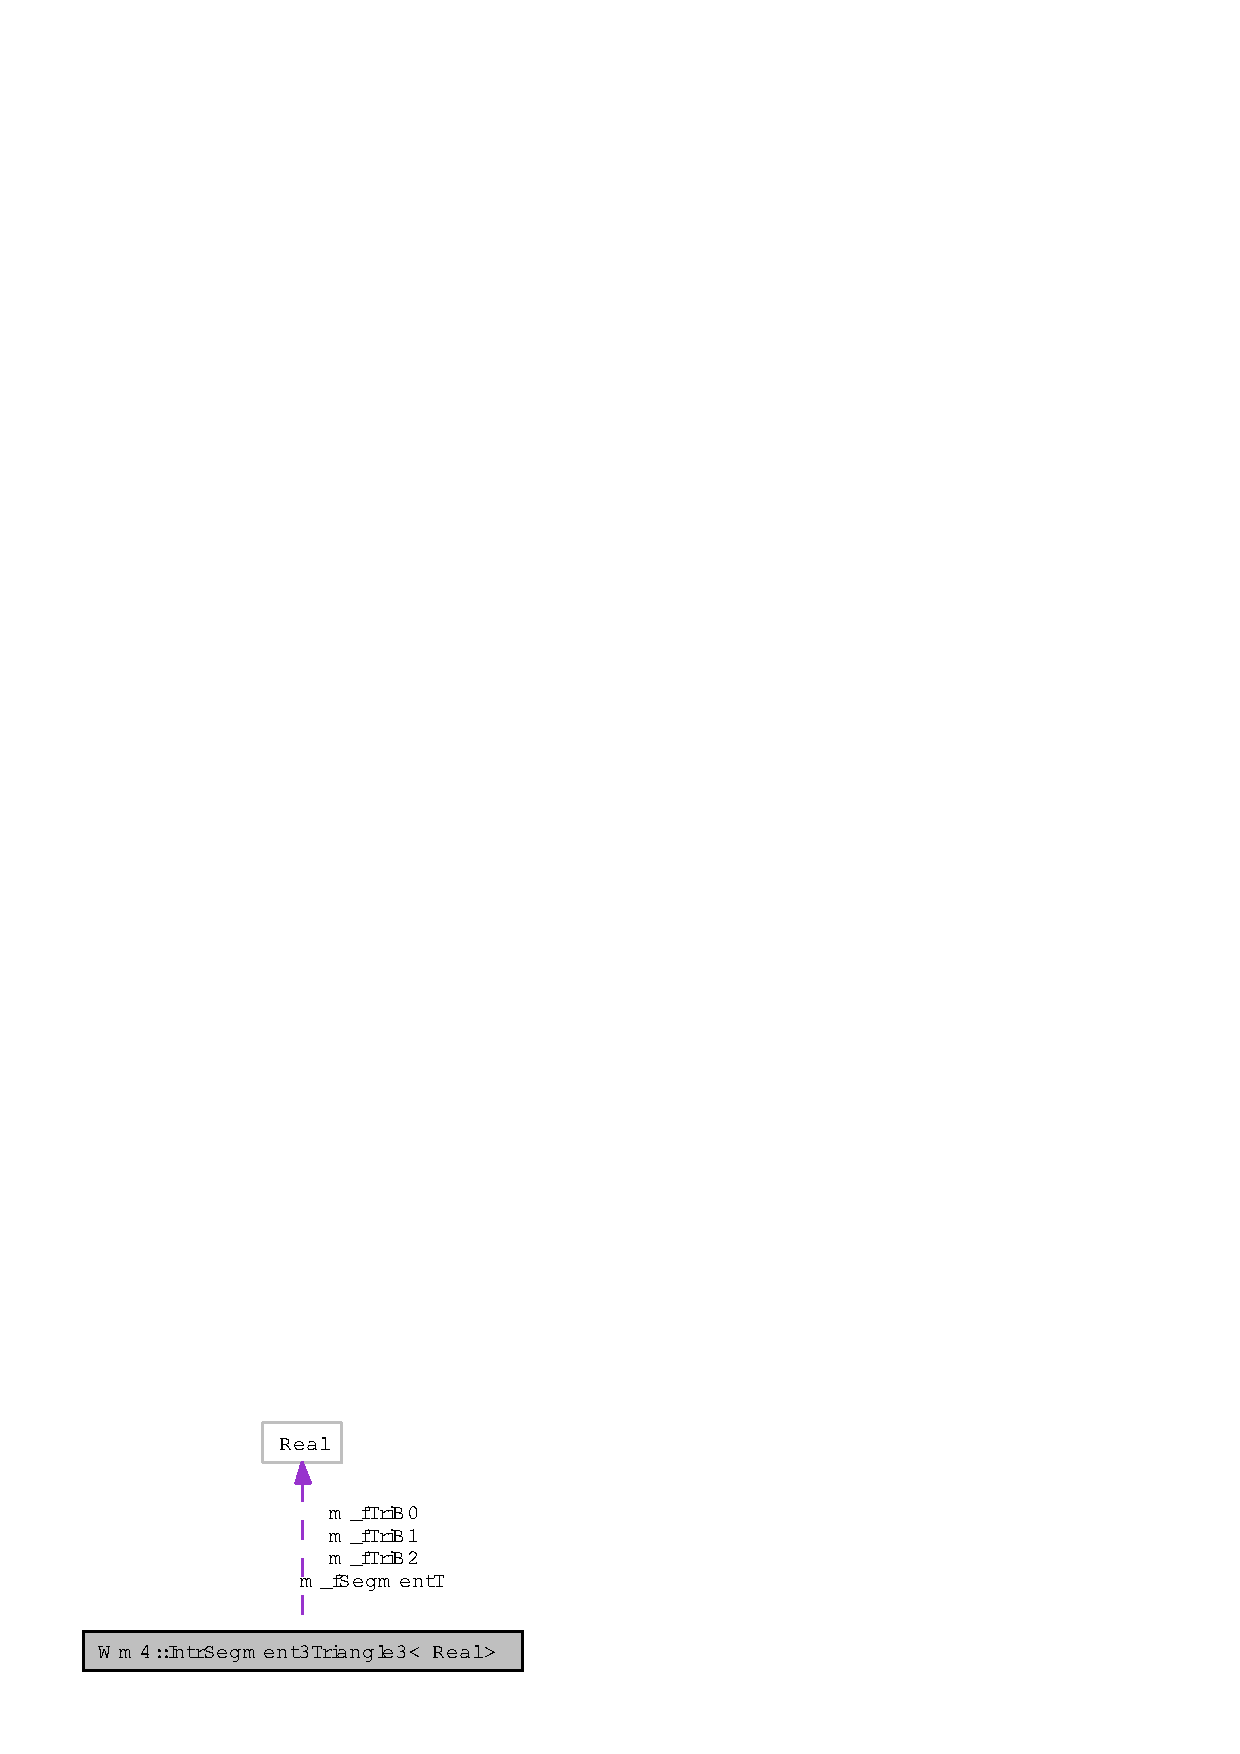
\includegraphics[width=127pt]{classWm4_1_1IntrSegment3Triangle3__coll__graph}
\end{center}
\end{figure}
\subsection*{Public Member Functions}
\begin{CompactItemize}
\item 
{\bf Intr\-Segment3Triangle3} (const Segment3$<$ Real $>$ \&rk\-Segment, const Triangle3$<$ Real $>$ \&rk\-Triangle)
\item 
const Segment3$<$ Real $>$ \& {\bf Get\-Segment} () const
\item 
const Triangle3$<$ Real $>$ \& {\bf Get\-Triangle} () const
\item 
virtual bool {\bf Test} ()
\item 
virtual bool {\bf Find} ()
\item 
Real {\bf Get\-Segment\-T} () const
\item 
Real {\bf Get\-Tri\-B0} () const
\item 
Real {\bf Get\-Tri\-B1} () const
\item 
Real {\bf Get\-Tri\-B2} () const
\item 
virtual bool {\bf Test} (Real f\-TMax, const {\bf Vector3}$<$ Real $>$ \&rk\-Velocity0, const {\bf Vector3}$<$ Real $>$ \&rk\-Velocity1)
\item 
virtual bool {\bf Find} (Real f\-TMax, const {\bf Vector3}$<$ Real $>$ \&rk\-Velocity0, const {\bf Vector3}$<$ Real $>$ \&rk\-Velocity1)
\item 
int {\bf Get\-Quantity} () const
\item 
const {\bf Vector3}$<$ Real $>$ \& {\bf Get\-Point} (int i) const
\end{CompactItemize}
\subsubsection*{template$<$class Real$>$ class Wm4::Intr\-Segment3Triangle3$<$ Real $>$}



\subsection{Constructor \& Destructor Documentation}
\index{Wm4::IntrSegment3Triangle3@{Wm4::Intr\-Segment3Triangle3}!IntrSegment3Triangle3@{IntrSegment3Triangle3}}
\index{IntrSegment3Triangle3@{IntrSegment3Triangle3}!Wm4::IntrSegment3Triangle3@{Wm4::Intr\-Segment3Triangle3}}
\subsubsection{\setlength{\rightskip}{0pt plus 5cm}template$<$class Real$>$ {\bf Wm4::Intr\-Segment3Triangle3}$<$ Real $>$::{\bf Intr\-Segment3Triangle3} (const Segment3$<$ Real $>$ \& {\em rk\-Segment}, const Triangle3$<$ Real $>$ \& {\em rk\-Triangle})}\label{classWm4_1_1IntrSegment3Triangle3_ae90a2770821bb24ea659d635c919176}




\subsection{Member Function Documentation}
\index{Wm4::IntrSegment3Triangle3@{Wm4::Intr\-Segment3Triangle3}!GetSegment@{GetSegment}}
\index{GetSegment@{GetSegment}!Wm4::IntrSegment3Triangle3@{Wm4::Intr\-Segment3Triangle3}}
\subsubsection{\setlength{\rightskip}{0pt plus 5cm}template$<$class Real$>$ const Segment3$<$ Real $>$ \& {\bf Wm4::Intr\-Segment3Triangle3}$<$ Real $>$::Get\-Segment () const}\label{classWm4_1_1IntrSegment3Triangle3_b32213d1a8556d80f3da862d80b78408}


\index{Wm4::IntrSegment3Triangle3@{Wm4::Intr\-Segment3Triangle3}!GetTriangle@{GetTriangle}}
\index{GetTriangle@{GetTriangle}!Wm4::IntrSegment3Triangle3@{Wm4::Intr\-Segment3Triangle3}}
\subsubsection{\setlength{\rightskip}{0pt plus 5cm}template$<$class Real$>$ const Triangle3$<$ Real $>$ \& {\bf Wm4::Intr\-Segment3Triangle3}$<$ Real $>$::Get\-Triangle () const}\label{classWm4_1_1IntrSegment3Triangle3_5cc684c2193aa0741761d32aef70e702}


\index{Wm4::IntrSegment3Triangle3@{Wm4::Intr\-Segment3Triangle3}!Test@{Test}}
\index{Test@{Test}!Wm4::IntrSegment3Triangle3@{Wm4::Intr\-Segment3Triangle3}}
\subsubsection{\setlength{\rightskip}{0pt plus 5cm}template$<$class Real$>$ bool {\bf Wm4::Intr\-Segment3Triangle3}$<$ Real $>$::Test ()\hspace{0.3cm}{\tt  [virtual]}}\label{classWm4_1_1IntrSegment3Triangle3_d4805ab9e7f40f421b7271ea057e2fcb}


\index{Wm4::IntrSegment3Triangle3@{Wm4::Intr\-Segment3Triangle3}!Find@{Find}}
\index{Find@{Find}!Wm4::IntrSegment3Triangle3@{Wm4::Intr\-Segment3Triangle3}}
\subsubsection{\setlength{\rightskip}{0pt plus 5cm}template$<$class Real$>$ bool {\bf Wm4::Intr\-Segment3Triangle3}$<$ Real $>$::Find ()\hspace{0.3cm}{\tt  [virtual]}}\label{classWm4_1_1IntrSegment3Triangle3_cbce364d2d648f6dc0628f28cf88b8b2}


\index{Wm4::IntrSegment3Triangle3@{Wm4::Intr\-Segment3Triangle3}!GetSegmentT@{GetSegmentT}}
\index{GetSegmentT@{GetSegmentT}!Wm4::IntrSegment3Triangle3@{Wm4::Intr\-Segment3Triangle3}}
\subsubsection{\setlength{\rightskip}{0pt plus 5cm}template$<$class Real$>$ Real {\bf Wm4::Intr\-Segment3Triangle3}$<$ Real $>$::Get\-Segment\-T () const}\label{classWm4_1_1IntrSegment3Triangle3_3c4873255c7a4bdf3d71f22c3d557118}


\index{Wm4::IntrSegment3Triangle3@{Wm4::Intr\-Segment3Triangle3}!GetTriB0@{GetTriB0}}
\index{GetTriB0@{GetTriB0}!Wm4::IntrSegment3Triangle3@{Wm4::Intr\-Segment3Triangle3}}
\subsubsection{\setlength{\rightskip}{0pt plus 5cm}template$<$class Real$>$ Real {\bf Wm4::Intr\-Segment3Triangle3}$<$ Real $>$::Get\-Tri\-B0 () const}\label{classWm4_1_1IntrSegment3Triangle3_e0552d572714bf9d22d2cd74c4362f9b}


\index{Wm4::IntrSegment3Triangle3@{Wm4::Intr\-Segment3Triangle3}!GetTriB1@{GetTriB1}}
\index{GetTriB1@{GetTriB1}!Wm4::IntrSegment3Triangle3@{Wm4::Intr\-Segment3Triangle3}}
\subsubsection{\setlength{\rightskip}{0pt plus 5cm}template$<$class Real$>$ Real {\bf Wm4::Intr\-Segment3Triangle3}$<$ Real $>$::Get\-Tri\-B1 () const}\label{classWm4_1_1IntrSegment3Triangle3_ffc0a298a3a668c7052fb9b29f70d754}


\index{Wm4::IntrSegment3Triangle3@{Wm4::Intr\-Segment3Triangle3}!GetTriB2@{GetTriB2}}
\index{GetTriB2@{GetTriB2}!Wm4::IntrSegment3Triangle3@{Wm4::Intr\-Segment3Triangle3}}
\subsubsection{\setlength{\rightskip}{0pt plus 5cm}template$<$class Real$>$ Real {\bf Wm4::Intr\-Segment3Triangle3}$<$ Real $>$::Get\-Tri\-B2 () const}\label{classWm4_1_1IntrSegment3Triangle3_e94f5488046b1331cf02f6a78618ffa4}


\index{Wm4::IntrSegment3Triangle3@{Wm4::Intr\-Segment3Triangle3}!Test@{Test}}
\index{Test@{Test}!Wm4::IntrSegment3Triangle3@{Wm4::Intr\-Segment3Triangle3}}
\subsubsection{\setlength{\rightskip}{0pt plus 5cm}template$<$class Real$>$ bool {\bf Wm4::Intr\-Segment3Triangle3}$<$ Real $>$::Test (Real {\em f\-TMax}, const {\bf Vector3}$<$ Real $>$ \& {\em rk\-Velocity0}, const {\bf Vector3}$<$ Real $>$ \& {\em rk\-Velocity1})\hspace{0.3cm}{\tt  [virtual]}}\label{classWm4_1_1IntrSegment3Triangle3_ec56edb6e1a5e4a3eab61b90d21d3180}


\index{Wm4::IntrSegment3Triangle3@{Wm4::Intr\-Segment3Triangle3}!Find@{Find}}
\index{Find@{Find}!Wm4::IntrSegment3Triangle3@{Wm4::Intr\-Segment3Triangle3}}
\subsubsection{\setlength{\rightskip}{0pt plus 5cm}template$<$class Real$>$ bool {\bf Wm4::Intr\-Segment3Triangle3}$<$ Real $>$::Find (Real {\em f\-TMax}, const {\bf Vector3}$<$ Real $>$ \& {\em rk\-Velocity0}, const {\bf Vector3}$<$ Real $>$ \& {\em rk\-Velocity1})\hspace{0.3cm}{\tt  [virtual]}}\label{classWm4_1_1IntrSegment3Triangle3_14b6137039fc467396424e8b5e6716aa}


\index{Wm4::IntrSegment3Triangle3@{Wm4::Intr\-Segment3Triangle3}!GetQuantity@{GetQuantity}}
\index{GetQuantity@{GetQuantity}!Wm4::IntrSegment3Triangle3@{Wm4::Intr\-Segment3Triangle3}}
\subsubsection{\setlength{\rightskip}{0pt plus 5cm}template$<$class Real$>$ int {\bf Wm4::Intr\-Segment3Triangle3}$<$ Real $>$::Get\-Quantity () const}\label{classWm4_1_1IntrSegment3Triangle3_1c9ecd76e19183d907ca8d57e864ed7b}


\index{Wm4::IntrSegment3Triangle3@{Wm4::Intr\-Segment3Triangle3}!GetPoint@{GetPoint}}
\index{GetPoint@{GetPoint}!Wm4::IntrSegment3Triangle3@{Wm4::Intr\-Segment3Triangle3}}
\subsubsection{\setlength{\rightskip}{0pt plus 5cm}template$<$class Real$>$ const {\bf Vector3}$<$ Real $>$ \& {\bf Wm4::Intr\-Segment3Triangle3}$<$ Real $>$::Get\-Point (int {\em i}) const}\label{classWm4_1_1IntrSegment3Triangle3_04684d5627edf7335bac7730cf4767a7}




The documentation for this class was generated from the following files:\begin{CompactItemize}
\item 
{\bf Wm4Intr\-Segment3Triangle3.h}\item 
{\bf Wm4Intr\-Segment3Triangle3.cpp}\end{CompactItemize}

\section{Wm4::Intr\-Triangle3Cone3$<$ Real $>$ Class Template Reference}
\label{classWm4_1_1IntrTriangle3Cone3}\index{Wm4::IntrTriangle3Cone3@{Wm4::IntrTriangle3Cone3}}
{\tt \#include $<$Wm4Intr\-Triangle3Cone3.h$>$}

\subsection*{Public Member Functions}
\begin{CompactItemize}
\item 
{\bf Intr\-Triangle3Cone3} (const Triangle3$<$ Real $>$ \&rk\-Triangle, const Cone3$<$ Real $>$ \&rk\-Cone)
\item 
const Triangle3$<$ Real $>$ \& {\bf Get\-Triangle} () const
\item 
const Cone3$<$ Real $>$ \& {\bf Get\-Cone} () const
\item 
virtual bool {\bf Test} ()
\end{CompactItemize}
\subsubsection*{template$<$class Real$>$ class Wm4::Intr\-Triangle3Cone3$<$ Real $>$}



\subsection{Constructor \& Destructor Documentation}
\index{Wm4::IntrTriangle3Cone3@{Wm4::Intr\-Triangle3Cone3}!IntrTriangle3Cone3@{IntrTriangle3Cone3}}
\index{IntrTriangle3Cone3@{IntrTriangle3Cone3}!Wm4::IntrTriangle3Cone3@{Wm4::Intr\-Triangle3Cone3}}
\subsubsection{\setlength{\rightskip}{0pt plus 5cm}template$<$class Real$>$ {\bf Wm4::Intr\-Triangle3Cone3}$<$ Real $>$::{\bf Intr\-Triangle3Cone3} (const Triangle3$<$ Real $>$ \& {\em rk\-Triangle}, const Cone3$<$ Real $>$ \& {\em rk\-Cone})}\label{classWm4_1_1IntrTriangle3Cone3_86caba9024ef7f4f202ec11627ea37e5}




\subsection{Member Function Documentation}
\index{Wm4::IntrTriangle3Cone3@{Wm4::Intr\-Triangle3Cone3}!GetTriangle@{GetTriangle}}
\index{GetTriangle@{GetTriangle}!Wm4::IntrTriangle3Cone3@{Wm4::Intr\-Triangle3Cone3}}
\subsubsection{\setlength{\rightskip}{0pt plus 5cm}template$<$class Real$>$ const Triangle3$<$ Real $>$ \& {\bf Wm4::Intr\-Triangle3Cone3}$<$ Real $>$::Get\-Triangle () const}\label{classWm4_1_1IntrTriangle3Cone3_620beb552e82511bcf2b67f1a1de220a}


\index{Wm4::IntrTriangle3Cone3@{Wm4::Intr\-Triangle3Cone3}!GetCone@{GetCone}}
\index{GetCone@{GetCone}!Wm4::IntrTriangle3Cone3@{Wm4::Intr\-Triangle3Cone3}}
\subsubsection{\setlength{\rightskip}{0pt plus 5cm}template$<$class Real$>$ const Cone3$<$ Real $>$ \& {\bf Wm4::Intr\-Triangle3Cone3}$<$ Real $>$::Get\-Cone () const}\label{classWm4_1_1IntrTriangle3Cone3_2a4d8302b291f20a934edeb305050e1e}


\index{Wm4::IntrTriangle3Cone3@{Wm4::Intr\-Triangle3Cone3}!Test@{Test}}
\index{Test@{Test}!Wm4::IntrTriangle3Cone3@{Wm4::Intr\-Triangle3Cone3}}
\subsubsection{\setlength{\rightskip}{0pt plus 5cm}template$<$class Real$>$ bool {\bf Wm4::Intr\-Triangle3Cone3}$<$ Real $>$::Test ()\hspace{0.3cm}{\tt  [virtual]}}\label{classWm4_1_1IntrTriangle3Cone3_e47fccb80478b76bb474ee8768fbacdd}




The documentation for this class was generated from the following files:\begin{CompactItemize}
\item 
{\bf Wm4Intr\-Triangle3Cone3.h}\item 
{\bf Wm4Intr\-Triangle3Cone3.cpp}\end{CompactItemize}

\section{Log Class Reference}
\label{classLog}\index{Log@{Log}}
{\tt \#include $<$log.h$>$}

Collaboration diagram for Log:\begin{figure}[H]
\begin{center}
\leavevmode
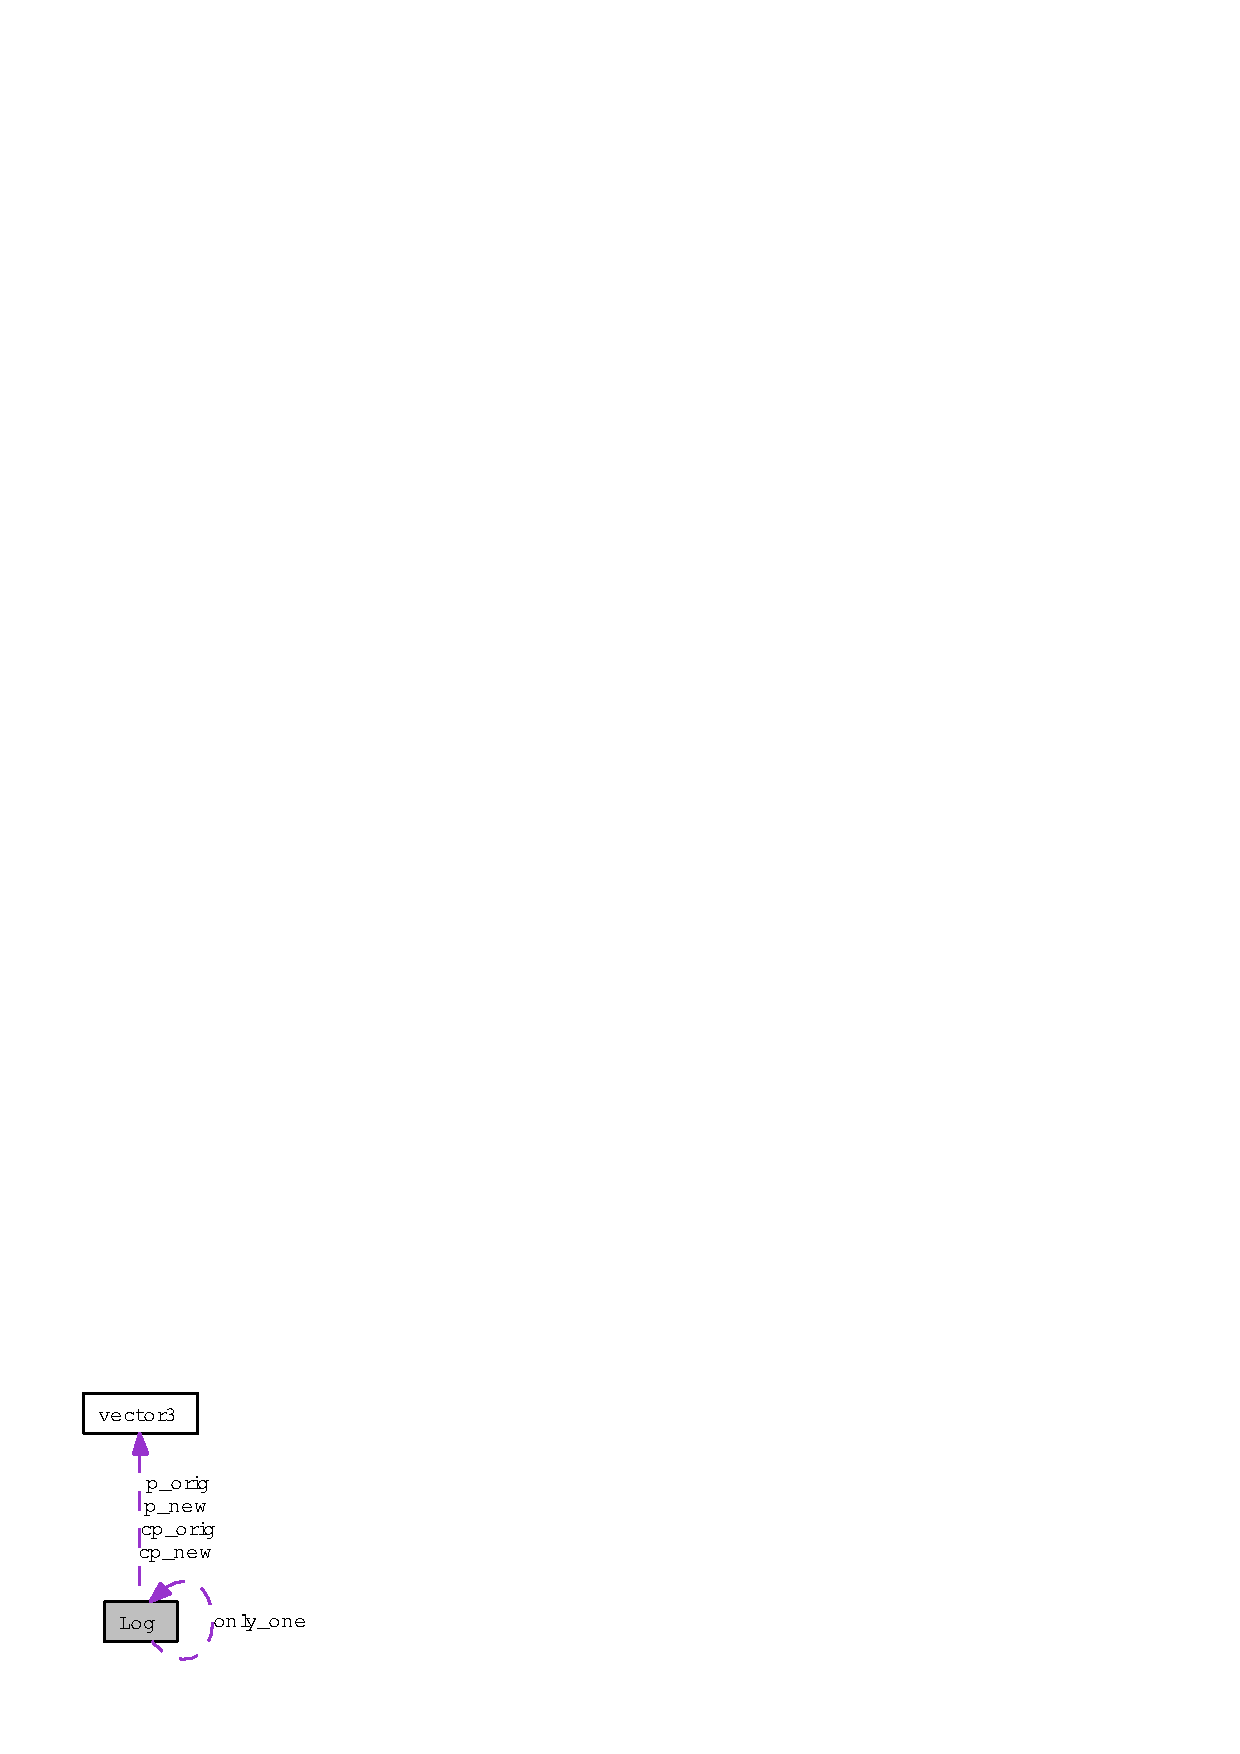
\includegraphics[width=76pt]{classLog__coll__graph}
\end{center}
\end{figure}
\subsection*{Public Member Functions}
\begin{CompactItemize}
\item 
int {\bf get\-N} (void)
\item 
void {\bf group\-Init} (void)
\item 
void {\bf write\-Vert\-Move\-Distribution} (int const \&)
\item 
void {\bf write\-Files} (int const \&group)
\item 
void {\bf write\-Sep\-Distances} (int const \&)
\item 
void {\bf update\-Hauss\_\-1} (std::string const \&, double const \&, {\bf map\_\-s\_\-d} \&)
\item 
void {\bf update\-Hauss\_\-2} (std::string const \&, {\bf o\_\-it} const \&, double const \&, {\bf map\_\-s\_\-d} \&)
\item 
void {\bf update\-Hauss\_\-1\_\-noself} (std::string const \&, double const \&, {\bf map\_\-s\_\-d} \&)
\item 
void {\bf update\-Hauss\_\-2\_\-noself} (std::string const \&, {\bf o\_\-it} const \&, double const \&, {\bf map\_\-s\_\-d} \&)
\item 
void {\bf write\-Command\-Settings} (void)
\item 
void {\bf close\-Files} (void)
\item 
void {\bf update\-File} (int const \&, bool, double const \&)
\item 
void {\bf status\-File\-Init} (void)
\item 
void {\bf write\-Object\-List} (void)
\item 
void {\bf write\-Object\-Data} (void)
\item 
void {\bf update\-Vert\-Displ\-Stats} ({\bf Vertex} $\ast$const, {\bf vector3} const \&)
\item 
void {\bf clear\-Vals} (void)
\item 
void {\bf write\-Move\-Summary} (int const \&, int const \&)
\item 
void {\bf write\-Refracted} (int const \&)
\item 
void {\bf write\-Refracted\-Now} (int const \&group, int code)
\item 
void {\bf write\-Intersected} (int const \&)
\item 
void {\bf write\-Nonnice} (int const \&)
\item 
void {\bf write\-VD} (int const \&)
\item 
void {\bf write\-AD} (int const \&group)
\item 
void {\bf print\-Num\-Nonnice} (std::ostream \&) const
\item 
void {\bf print\-Num\-Int} (std::ostream \&) const
\item 
void {\bf set\-Time} (time\_\-t)
\item 
void {\bf open\-Main\-File} (void)
\item 
void {\bf record\-Time} (std::string const \&)
\item 
void {\bf update\-Boxes\-Per\-Face\-Stats} (int const \&)
\item 
void {\bf calculate\-Faces\-Per\-Box\-Stats} (void)
\item 
void {\bf print\-Partitioning\-Stats} (std::ostream \&) const
\item 
void {\bf update\-Closest\-Pt\-Stats} (int const \&, int const \&, int const \&)
\item 
void {\bf print\-Closest\-Pt\-Stats} (std::ostream \&) const
\item 
void {\bf update\-Vertex\-Scheduling\-Stats} (int const \&)
\item 
void {\bf update\-Moved\-Verts\-From\-Set} (void)
\item 
void {\bf print\-Vertex\-Scheduling\-Stats} (std::ostream \&) const
\item 
void {\bf update\-Closest\-Pt\-Search\-Stats} (int const \&, int const \&, {\bf Search\_\-Stats} const \&)
\item 
void {\bf print\-Closest\-Pt\-Search\-Stats} (std::ostream \&) const
\item 
void {\bf open\-Or\-Die} (std::ofstream $\ast$const handle, std::string str, const int \&group)
\item 
bool {\bf is\-Good} ({\bf Vertex} const $\ast$const) const 
\item 
void {\bf write\-Detailed\-Move\-Info} (void)
\item 
void {\bf print\-Bad} ({\bf Vertex} const $\ast$const) const 
\item 
void {\bf set\-Detailed\-Info\-Pre\-Move} ({\bf Vertex} $\ast$const)
\item 
void {\bf set\-Detailed\-Info\-Post\-Move} ({\bf Vertex} $\ast$)
\item 
std::string {\bf formatv} (char const $\ast$fmt, va\_\-list args)
\item 
std::string {\bf format} (char const $\ast$fmt,...)
\end{CompactItemize}
\subsection*{Static Public Member Functions}
\begin{CompactItemize}
\item 
static {\bf Log} \& {\bf instance} (void)
\end{CompactItemize}


\subsection{Member Function Documentation}
\index{Log@{Log}!instance@{instance}}
\index{instance@{instance}!Log@{Log}}
\subsubsection{\setlength{\rightskip}{0pt plus 5cm}{\bf Log} \& Log::instance (void)\hspace{0.3cm}{\tt  [static]}}\label{classLog_560f0bdc9894198be1466c9888acb6fe}


\index{Log@{Log}!getN@{getN}}
\index{getN@{getN}!Log@{Log}}
\subsubsection{\setlength{\rightskip}{0pt plus 5cm}int Log::get\-N (void)\hspace{0.3cm}{\tt  [inline]}}\label{classLog_5984805af8f02565ce88ae6156e0dbaf}


\index{Log@{Log}!groupInit@{groupInit}}
\index{groupInit@{groupInit}!Log@{Log}}
\subsubsection{\setlength{\rightskip}{0pt plus 5cm}void Log::group\-Init (void)}\label{classLog_5a5bf6231b9a3af27a535bfe60307b55}


Initialize this class for start of group. \index{Log@{Log}!writeVertMoveDistribution@{writeVertMoveDistribution}}
\index{writeVertMoveDistribution@{writeVertMoveDistribution}!Log@{Log}}
\subsubsection{\setlength{\rightskip}{0pt plus 5cm}void Log::write\-Vert\-Move\-Distribution (int const \& {\em group})}\label{classLog_0c4b2a52477b8c929cb4c05d4d27793e}


Write to file the distribution of number of moves per vertex since start of last initialization. \begin{Desc}
\item[Parameters:]
\begin{description}
\item[\mbox{$\leftarrow$} {\em group}]Current group number (used as filename suffix). \end{description}
\end{Desc}
\index{Log@{Log}!writeFiles@{writeFiles}}
\index{writeFiles@{writeFiles}!Log@{Log}}
\subsubsection{\setlength{\rightskip}{0pt plus 5cm}void Log::write\-Files (int const \& {\em group})}\label{classLog_4ad9b818e3bc06dc1adfc9d79f29cb50}


Write to file the current position of model and diagnostic data. \begin{Desc}
\item[Parameters:]
\begin{description}
\item[\mbox{$\leftarrow$} {\em group}]Current group number. \end{description}
\end{Desc}
\index{Log@{Log}!writeSepDistances@{writeSepDistances}}
\index{writeSepDistances@{writeSepDistances}!Log@{Log}}
\subsubsection{\setlength{\rightskip}{0pt plus 5cm}void Log::write\-Sep\-Distances (int const \& {\em group})}\label{classLog_8bd4f014fe08393caf59f9f29ac75d36}


Calculate and write to file the extracellular width (or some metric) of each vertex in model using the stored closest face. \begin{Desc}
\item[Parameters:]
\begin{description}
\item[\mbox{$\leftarrow$} {\em group}]Current group number (used as filename suffix). \end{description}
\end{Desc}
\index{Log@{Log}!updateHauss_1@{updateHauss\_\-1}}
\index{updateHauss_1@{updateHauss\_\-1}!Log@{Log}}
\subsubsection{\setlength{\rightskip}{0pt plus 5cm}void Log::update\-Hauss\_\-1 (std::string const \& {\em name}, double const \& {\em dd}, {\bf map\_\-s\_\-d} \& {\em hausdorff\_\-1})}\label{classLog_19fed1d607f1b2b3c2df3cdeec659eb7}


Determine if extracellular distance to object is to be stored. \begin{Desc}
\item[Parameters:]
\begin{description}
\item[\mbox{$\leftarrow$} {\em name}]Identity of neighboring object. \item[\mbox{$\leftarrow$} {\em dd}]Extracellular distance to object. \item[\mbox{$\rightarrow$} {\em hausdorff\_\-1}]Map of neighboring objects and associated extracellular widths. \end{description}
\end{Desc}
\index{Log@{Log}!updateHauss_2@{updateHauss\_\-2}}
\index{updateHauss_2@{updateHauss\_\-2}!Log@{Log}}
\subsubsection{\setlength{\rightskip}{0pt plus 5cm}void Log::update\-Hauss\_\-2 (std::string const \& {\em name}, {\bf o\_\-it} const \& {\em i}, double const \& {\em dd}, {\bf map\_\-s\_\-d} \& {\em hausdorff\_\-2})}\label{classLog_132325fad016ba2a8d16af4fef52d32d}


Determine if extracellular distance to object is to be stored. \begin{Desc}
\item[Parameters:]
\begin{description}
\item[\mbox{$\leftarrow$} {\em name}]Identity of neighboring object. \item[\mbox{$\leftarrow$} {\em i}]\doxyref{Object}{p.}{classObject} of interest. \item[\mbox{$\leftarrow$} {\em dd}]Extracellular distance to object. \item[\mbox{$\rightarrow$} {\em hausdorff\_\-2}]Map of neighboring objects and associated extracellular widths. \end{description}
\end{Desc}
\index{Log@{Log}!updateHauss_1_noself@{updateHauss\_\-1\_\-noself}}
\index{updateHauss_1_noself@{updateHauss\_\-1\_\-noself}!Log@{Log}}
\subsubsection{\setlength{\rightskip}{0pt plus 5cm}void Log::update\-Hauss\_\-1\_\-noself (std::string const \& {\em name}, double const \& {\em dd}, {\bf map\_\-s\_\-d} \& {\em hausdorff\_\-1\_\-noself})}\label{classLog_c86f0bab9e01d29b4e2f52cd7c3a82a6}


Determine if extracellular distance to object is to be stored. \begin{Desc}
\item[Parameters:]
\begin{description}
\item[\mbox{$\leftarrow$} {\em name}]Identity of neighboring object. \item[\mbox{$\leftarrow$} {\em dd}]Extracellular distance to object. \item[\mbox{$\rightarrow$} {\em hausdorff\_\-1\_\-noself}]Map of neighboring objects and associated extracellular widths. \end{description}
\end{Desc}
\index{Log@{Log}!updateHauss_2_noself@{updateHauss\_\-2\_\-noself}}
\index{updateHauss_2_noself@{updateHauss\_\-2\_\-noself}!Log@{Log}}
\subsubsection{\setlength{\rightskip}{0pt plus 5cm}void Log::update\-Hauss\_\-2\_\-noself (std::string const \& {\em name}, {\bf o\_\-it} const \& {\em i}, double const \& {\em dd}, {\bf map\_\-s\_\-d} \& {\em hausdorff\_\-2\_\-noself})}\label{classLog_5084b574cf76ccd39801c09981539815}


Determine if extracellular distance to object is to be stored. \begin{Desc}
\item[Parameters:]
\begin{description}
\item[\mbox{$\leftarrow$} {\em name}]Identity of neighboring object. \item[\mbox{$\leftarrow$} {\em i}]\doxyref{Object}{p.}{classObject} of interest. \item[\mbox{$\leftarrow$} {\em dd}]Extracellular distance to object. \item[\mbox{$\rightarrow$} {\em hausdorff\_\-2\_\-noself}]Map of neighboring objects and associated extracellular widths. \end{description}
\end{Desc}
\index{Log@{Log}!writeCommandSettings@{writeCommandSettings}}
\index{writeCommandSettings@{writeCommandSettings}!Log@{Log}}
\subsubsection{\setlength{\rightskip}{0pt plus 5cm}void Log::write\-Command\-Settings (void)}\label{classLog_aea40113d8b8f95f34b54e694bfc9b3f}


Write command parameter settings to file. \index{Log@{Log}!closeFiles@{closeFiles}}
\index{closeFiles@{closeFiles}!Log@{Log}}
\subsubsection{\setlength{\rightskip}{0pt plus 5cm}void Log::close\-Files (void)}\label{classLog_ccaa869ade8e961337493d61eae74228}


Close output streams of this class. \index{Log@{Log}!updateFile@{updateFile}}
\index{updateFile@{updateFile}!Log@{Log}}
\subsubsection{\setlength{\rightskip}{0pt plus 5cm}void Log::update\-File (int const \& {\em group}, bool {\em verts\_\-moved}, double const \& {\em elapsed\_\-time})}\label{classLog_1ef9d68100fee4568c43e58660eac593}


Write to file the progress of vertex move campaign. \begin{Desc}
\item[Parameters:]
\begin{description}
\item[\mbox{$\leftarrow$} {\em group}]Current group number. \item[\mbox{$\leftarrow$} {\em not\_\-first\_\-group}]True if group is NOT the first group; false otherwise. \item[\mbox{$\leftarrow$} {\em elapsed\_\-time}]Elapsed time since last initialization. \end{description}
\end{Desc}
\index{Log@{Log}!statusFileInit@{statusFileInit}}
\index{statusFileInit@{statusFileInit}!Log@{Log}}
\subsubsection{\setlength{\rightskip}{0pt plus 5cm}void Log::status\-File\-Init (void)}\label{classLog_2b40ac1a684072ebe0ff13be2f6e638b}


Initialize progress file for vertex move campaign. \index{Log@{Log}!writeObjectList@{writeObjectList}}
\index{writeObjectList@{writeObjectList}!Log@{Log}}
\subsubsection{\setlength{\rightskip}{0pt plus 5cm}void Log::write\-Object\-List (void)}\label{classLog_1886bc499dbcb83a87e29c31c6aad6b3}


Write to file a list of objects in model. \index{Log@{Log}!writeObjectData@{writeObjectData}}
\index{writeObjectData@{writeObjectData}!Log@{Log}}
\subsubsection{\setlength{\rightskip}{0pt plus 5cm}void Log::write\-Object\-Data (void)}\label{classLog_6196328a2b244940b90e0931c975be0d}


Write to file the object list and initialize the vertex move campaing progress file. \index{Log@{Log}!updateVertDisplStats@{updateVertDisplStats}}
\index{updateVertDisplStats@{updateVertDisplStats}!Log@{Log}}
\subsubsection{\setlength{\rightskip}{0pt plus 5cm}void Log::update\-Vert\-Displ\-Stats ({\bf Vertex} $\ast$ const {\em v}, {\bf vector3} const \& {\em old\_\-pos})}\label{classLog_7f1e317915f4f4f0c81e67760f54fb37}


Update statistics on actual vertex displacements. \begin{Desc}
\item[Parameters:]
\begin{description}
\item[\mbox{$\leftarrow$} {\em vertex\_\-displ}]Most recent vertex displacement. \end{description}
\end{Desc}
\index{Log@{Log}!clearVals@{clearVals}}
\index{clearVals@{clearVals}!Log@{Log}}
\subsubsection{\setlength{\rightskip}{0pt plus 5cm}void Log::clear\-Vals (void)}\label{classLog_b9a9ee2553ef9a26e303b91b37bf26bf}


Clear members of this class. \index{Log@{Log}!writeMoveSummary@{writeMoveSummary}}
\index{writeMoveSummary@{writeMoveSummary}!Log@{Log}}
\subsubsection{\setlength{\rightskip}{0pt plus 5cm}void Log::write\-Move\-Summary (int const \& {\em group}, int const \& {\em group\_\-size})}\label{classLog_5fe038c98dd24c85d2347bea8ca914a3}


Write to STDOUT a brief summary information about the last vertex move. \begin{Desc}
\item[Parameters:]
\begin{description}
\item[\mbox{$\leftarrow$} {\em group}]Current group number (used as filename suffix). \end{description}
\end{Desc}
\index{Log@{Log}!writeRefracted@{writeRefracted}}
\index{writeRefracted@{writeRefracted}!Log@{Log}}
\subsubsection{\setlength{\rightskip}{0pt plus 5cm}void Log::write\-Refracted (int const \& {\em group})}\label{classLog_7bcb3783a04992d550886708464f0dc7}


Write to file all vertices refracted since last initialization. \begin{Desc}
\item[Parameters:]
\begin{description}
\item[\mbox{$\leftarrow$} {\em group}]Current group number (used as filename suffix). \end{description}
\end{Desc}
\index{Log@{Log}!writeRefractedNow@{writeRefractedNow}}
\index{writeRefractedNow@{writeRefractedNow}!Log@{Log}}
\subsubsection{\setlength{\rightskip}{0pt plus 5cm}void Log::write\-Refracted\-Now (int const \& {\em group}, int {\em code})}\label{classLog_c3ba8bdae8fe2d2a9ff32400f5bb49c8}


\index{Log@{Log}!writeIntersected@{writeIntersected}}
\index{writeIntersected@{writeIntersected}!Log@{Log}}
\subsubsection{\setlength{\rightskip}{0pt plus 5cm}void Log::write\-Intersected (int const \& {\em group})}\label{classLog_a715ed09d236057bf460116a8f838003}


Write to file all intersected faces in model. \begin{Desc}
\item[Parameters:]
\begin{description}
\item[\mbox{$\leftarrow$} {\em group}]Current group number (used as filename suffix). \end{description}
\end{Desc}
\index{Log@{Log}!writeNonnice@{writeNonnice}}
\index{writeNonnice@{writeNonnice}!Log@{Log}}
\subsubsection{\setlength{\rightskip}{0pt plus 5cm}void Log::write\-Nonnice (int const \& {\em group})}\label{classLog_199cfdb352f8e095386f8573f063cd6b}


Write to file list of nonnice vertices in model. \begin{Desc}
\item[Parameters:]
\begin{description}
\item[\mbox{$\leftarrow$} {\em group}]Current group number (used as filename suffix). \end{description}
\end{Desc}
\index{Log@{Log}!writeVD@{writeVD}}
\index{writeVD@{writeVD}!Log@{Log}}
\subsubsection{\setlength{\rightskip}{0pt plus 5cm}void Log::write\-VD (int const \& {\em group})}\label{classLog_7ef40d818c36bf8a35ef66b198ba7a9f}


Write to file list of seed vertex virtual displacements. \begin{Desc}
\item[Parameters:]
\begin{description}
\item[\mbox{$\leftarrow$} {\em group}]Current group number (used as filename suffix). \end{description}
\end{Desc}
\index{Log@{Log}!writeAD@{writeAD}}
\index{writeAD@{writeAD}!Log@{Log}}
\subsubsection{\setlength{\rightskip}{0pt plus 5cm}void Log::write\-AD (int const \& {\em group})}\label{classLog_a2dc9da596fea7429c00a150b59477f7}


Write to file list of seed vertex virtual displacements. \begin{Desc}
\item[Parameters:]
\begin{description}
\item[\mbox{$\leftarrow$} {\em group}]Current group number (used as filename suffix). \end{description}
\end{Desc}
\index{Log@{Log}!printNumNonnice@{printNumNonnice}}
\index{printNumNonnice@{printNumNonnice}!Log@{Log}}
\subsubsection{\setlength{\rightskip}{0pt plus 5cm}void Log::print\-Num\-Nonnice (std::ostream \& {\em target}) const}\label{classLog_1e09afe77ce542420db47b5aeafc8cb2}


Write to output stream the number of vertices recorded nonnice.

\begin{Desc}
\item[Parameters:]
\begin{description}
\item[\mbox{$\leftarrow$} {\em target}]Pre-initialized output stream. \end{description}
\end{Desc}
\index{Log@{Log}!printNumInt@{printNumInt}}
\index{printNumInt@{printNumInt}!Log@{Log}}
\subsubsection{\setlength{\rightskip}{0pt plus 5cm}void Log::print\-Num\-Int (std::ostream \& {\em target}) const}\label{classLog_afffe6351bfe96546a9566ea180b5da2}


Write to output stream the number of faces recorded as intersected.

\begin{Desc}
\item[Parameters:]
\begin{description}
\item[\mbox{$\leftarrow$} {\em target}]Pre-initialized output stream. \end{description}
\end{Desc}
\index{Log@{Log}!setTime@{setTime}}
\index{setTime@{setTime}!Log@{Log}}
\subsubsection{\setlength{\rightskip}{0pt plus 5cm}void Log::set\-Time (time\_\-t {\em t})}\label{classLog_6b1c1f2e8eba5b16cc15b3ab925372ec}


Initialize time to input value. \begin{Desc}
\item[Parameters:]
\begin{description}
\item[\mbox{$\leftarrow$} {\em t}]New time value. \end{description}
\end{Desc}
\index{Log@{Log}!openMainFile@{openMainFile}}
\index{openMainFile@{openMainFile}!Log@{Log}}
\subsubsection{\setlength{\rightskip}{0pt plus 5cm}void Log::open\-Main\-File (void)}\label{classLog_2bb3d9606ea67f1f576a620c921a101b}


Initialize output stream to main log file. \index{Log@{Log}!recordTime@{recordTime}}
\index{recordTime@{recordTime}!Log@{Log}}
\subsubsection{\setlength{\rightskip}{0pt plus 5cm}void Log::record\-Time (std::string const \& {\em message})}\label{classLog_c4a10bd3cfa75164ed1a202f059b5e15}


Write to file elapsed time since last call of this function. \begin{Desc}
\item[Parameters:]
\begin{description}
\item[\mbox{$\leftarrow$} {\em message}]Message to write to file. \end{description}
\end{Desc}
\index{Log@{Log}!updateBoxesPerFaceStats@{updateBoxesPerFaceStats}}
\index{updateBoxesPerFaceStats@{updateBoxesPerFaceStats}!Log@{Log}}
\subsubsection{\setlength{\rightskip}{0pt plus 5cm}void Log::update\-Boxes\-Per\-Face\-Stats (int const \& {\em box\_\-count})}\label{classLog_a41d65fb13feb0e44735882ed9248cab}


Update statistics on the number of boxes assigned to each face. \begin{Desc}
\item[Parameters:]
\begin{description}
\item[\mbox{$\leftarrow$} {\em box\_\-count}]Number of space partitions assigned to this face. \end{description}
\end{Desc}
\index{Log@{Log}!calculateFacesPerBoxStats@{calculateFacesPerBoxStats}}
\index{calculateFacesPerBoxStats@{calculateFacesPerBoxStats}!Log@{Log}}
\subsubsection{\setlength{\rightskip}{0pt plus 5cm}void Log::calculate\-Faces\-Per\-Box\-Stats (void)}\label{classLog_a652c5b694b6857cb36a1470c0634407}


\index{Log@{Log}!printPartitioningStats@{printPartitioningStats}}
\index{printPartitioningStats@{printPartitioningStats}!Log@{Log}}
\subsubsection{\setlength{\rightskip}{0pt plus 5cm}void Log::print\-Partitioning\-Stats (std::ostream \& {\em target}) const}\label{classLog_5528e95549c8af74a0f1563de8b98a3e}


Write to output stream recorded statistics of the number of faces assigned to each box and the number of boxes assigned to each face. \begin{Desc}
\item[Parameters:]
\begin{description}
\item[\mbox{$\leftarrow$} {\em target}]Pre-initialized output stream. \end{description}
\end{Desc}
\index{Log@{Log}!updateClosestPtStats@{updateClosestPtStats}}
\index{updateClosestPtStats@{updateClosestPtStats}!Log@{Log}}
\subsubsection{\setlength{\rightskip}{0pt plus 5cm}void Log::update\-Closest\-Pt\-Stats (int const \& {\em face\_\-count}, int const \& {\em leaves\_\-count}, int const \& {\em f\_\-check\_\-count})}\label{classLog_a459ccc43f3789e41818528aa25c2dc5}


Gather statistics on number of faces and boxes invloved in search for closest point to each vertex. \begin{Desc}
\item[Parameters:]
\begin{description}
\item[\mbox{$\leftarrow$} {\em face\_\-count}]Number of faces returned from octree in last search for closest point to current vertex. \item[\mbox{$\leftarrow$} {\em leaves\_\-count}]Number of leaves checked in last search for closest point to current vertex. \item[\mbox{$\leftarrow$} {\em f\_\-check\_\-count}]Number of faces checked in last search for closest point to current vertex. \end{description}
\end{Desc}
\index{Log@{Log}!printClosestPtStats@{printClosestPtStats}}
\index{printClosestPtStats@{printClosestPtStats}!Log@{Log}}
\subsubsection{\setlength{\rightskip}{0pt plus 5cm}void Log::print\-Closest\-Pt\-Stats (std::ostream \& {\em target}) const}\label{classLog_5c3cd6d1108c12a47894bd7eac337236}


Write to output stream summary statistics for closest point to vertex searches.

\begin{Desc}
\item[Parameters:]
\begin{description}
\item[\mbox{$\leftarrow$} {\em target}]Pre-initialized output stream. \end{description}
\end{Desc}
\index{Log@{Log}!updateVertexSchedulingStats@{updateVertexSchedulingStats}}
\index{updateVertexSchedulingStats@{updateVertexSchedulingStats}!Log@{Log}}
\subsubsection{\setlength{\rightskip}{0pt plus 5cm}void Log::update\-Vertex\-Scheduling\-Stats (int const \& {\em vertex\_\-count})}\label{classLog_f78d560b9bbc18e24368eefb10d40427}


Update statistics on number of vertices per moved set. \begin{Desc}
\item[Parameters:]
\begin{description}
\item[\mbox{$\leftarrow$} {\em vertex\_\-count}]Number of vertices in last moved set (noting that not all vertices in a moved set are allowed to move). \end{description}
\end{Desc}
\index{Log@{Log}!updateMovedVertsFromSet@{updateMovedVertsFromSet}}
\index{updateMovedVertsFromSet@{updateMovedVertsFromSet}!Log@{Log}}
\subsubsection{\setlength{\rightskip}{0pt plus 5cm}void Log::update\-Moved\-Verts\-From\-Set (void)}\label{classLog_2385a5c845a5ca0c887c332b11cdf5c0}


Update statistics on number of vertices per moved set. (noting that not all vertices in a moved set are allowed to move). \index{Log@{Log}!printVertexSchedulingStats@{printVertexSchedulingStats}}
\index{printVertexSchedulingStats@{printVertexSchedulingStats}!Log@{Log}}
\subsubsection{\setlength{\rightskip}{0pt plus 5cm}void Log::print\-Vertex\-Scheduling\-Stats (std::ostream \& {\em target}) const}\label{classLog_445ff1de967f5ab8cb153b4a2aaa3909}


Write to output streqam statistics on number of vertices per moved set. \begin{Desc}
\item[Parameters:]
\begin{description}
\item[\mbox{$\leftarrow$} {\em target}]Pre-initialized output stream. \end{description}
\end{Desc}
\index{Log@{Log}!updateClosestPtSearchStats@{updateClosestPtSearchStats}}
\index{updateClosestPtSearchStats@{updateClosestPtSearchStats}!Log@{Log}}
\subsubsection{\setlength{\rightskip}{0pt plus 5cm}void Log::update\-Closest\-Pt\-Search\-Stats (int const \& {\em full\_\-search}, int const \& {\em partial\_\-search}, {\bf Search\_\-Stats} const \& {\em ss})}\label{classLog_a4c94a78f7826121a2e41133198d6421}


Gather statistics on number of vertices undergoing full and partial closest point searches. \begin{Desc}
\item[Parameters:]
\begin{description}
\item[\mbox{$\leftarrow$} {\em full\_\-search}]Number of vertices given a full closest point seach. \item[\mbox{$\leftarrow$} {\em partial\_\-search}]Number of vertices given a partial closest point seach. \item[\mbox{$\leftarrow$} {\em ss}]Collection of vertex counts quantifying how often the closest face to vertex changed. \end{description}
\end{Desc}
\index{Log@{Log}!printClosestPtSearchStats@{printClosestPtSearchStats}}
\index{printClosestPtSearchStats@{printClosestPtSearchStats}!Log@{Log}}
\subsubsection{\setlength{\rightskip}{0pt plus 5cm}void Log::print\-Closest\-Pt\-Search\-Stats (std::ostream \& {\em target}) const}\label{classLog_234e14eb8839970087544b86725a4b5e}


Write to output stream summary statistics for closest point to vertex searches.

\begin{Desc}
\item[Parameters:]
\begin{description}
\item[\mbox{$\leftarrow$} {\em target}]Pre-initialized output stream. \end{description}
\end{Desc}
\index{Log@{Log}!openOrDie@{openOrDie}}
\index{openOrDie@{openOrDie}!Log@{Log}}
\subsubsection{\setlength{\rightskip}{0pt plus 5cm}void Log::open\-Or\-Die (std::ofstream $\ast$const  {\em handle}, std::string {\em str}, const int \& {\em group})}\label{classLog_5c75edbcb518da9f8a22d4958e79d950}


\index{Log@{Log}!isGood@{isGood}}
\index{isGood@{isGood}!Log@{Log}}
\subsubsection{\setlength{\rightskip}{0pt plus 5cm}bool Log::is\-Good ({\bf Vertex} const $\ast$ const {\em current\_\-vertex}) const}\label{classLog_eff9b0e33dcc37e71c4b2bb6d9ce0ca1}


Assert values are inside valid range for class elements carring detailed vertex move information. \begin{Desc}
\item[Parameters:]
\begin{description}
\item[\mbox{$\leftarrow$} {\em current\_\-vertex}]\doxyref{Vertex}{p.}{classVertex} of interest, likely, the last vertex moved. \end{description}
\end{Desc}
\index{Log@{Log}!writeDetailedMoveInfo@{writeDetailedMoveInfo}}
\index{writeDetailedMoveInfo@{writeDetailedMoveInfo}!Log@{Log}}
\subsubsection{\setlength{\rightskip}{0pt plus 5cm}void Log::write\-Detailed\-Move\-Info (void)}\label{classLog_88f866427eb6e6c0a3cdd2fc316b41e5}


Write to STDOUT detailed information about last vertex move. \index{Log@{Log}!printBad@{printBad}}
\index{printBad@{printBad}!Log@{Log}}
\subsubsection{\setlength{\rightskip}{0pt plus 5cm}void Log::print\-Bad ({\bf Vertex} const $\ast$ const {\em current\_\-vertex}) const}\label{classLog_ea54bf1684e3b2a0b6a98ef8370bbf26}


Write to STDOUT debug data for vertex move detailed information. \index{Log@{Log}!setDetailedInfoPreMove@{setDetailedInfoPreMove}}
\index{setDetailedInfoPreMove@{setDetailedInfoPreMove}!Log@{Log}}
\subsubsection{\setlength{\rightskip}{0pt plus 5cm}void Log::set\-Detailed\-Info\-Pre\-Move ({\bf Vertex} $\ast$ const {\em v})}\label{classLog_5f75777cf5cb63898440900547696cfa}


Record detailed move information of current vertex before the move is attempted. \begin{Desc}
\item[Parameters:]
\begin{description}
\item[\mbox{$\leftarrow$} {\em v}]\doxyref{Vertex}{p.}{classVertex} to be moved. \end{description}
\end{Desc}
\index{Log@{Log}!setDetailedInfoPostMove@{setDetailedInfoPostMove}}
\index{setDetailedInfoPostMove@{setDetailedInfoPostMove}!Log@{Log}}
\subsubsection{\setlength{\rightskip}{0pt plus 5cm}void Log::set\-Detailed\-Info\-Post\-Move ({\bf Vertex} $\ast$ {\em v})}\label{classLog_ee0b4b55384422c4ae23ebdb03f94c6d}


Record detailed move information of current vertex after a successfuly move is made. \begin{Desc}
\item[Parameters:]
\begin{description}
\item[\mbox{$\leftarrow$} {\em v}]Last vertex moved. \end{description}
\end{Desc}
\index{Log@{Log}!formatv@{formatv}}
\index{formatv@{formatv}!Log@{Log}}
\subsubsection{\setlength{\rightskip}{0pt plus 5cm}std::string Log::formatv (char const $\ast$ {\em fmt}, va\_\-list {\em args})\hspace{0.3cm}{\tt  [inline]}}\label{classLog_75750275e5424749ae3a5e118e0635c1}


\index{Log@{Log}!format@{format}}
\index{format@{format}!Log@{Log}}
\subsubsection{\setlength{\rightskip}{0pt plus 5cm}std::string Log::format (char const $\ast$ {\em fmt},  {\em ...})\hspace{0.3cm}{\tt  [inline]}}\label{classLog_6713dfaa81b6c577ba3d2de6925480f9}




The documentation for this class was generated from the following files:\begin{CompactItemize}
\item 
{\bf log.h}\item 
{\bf log.cc}\end{CompactItemize}

\section{Wm4::Math$<$ Real $>$ Class Template Reference}
\label{classWm4_1_1Math}\index{Wm4::Math@{Wm4::Math}}
{\tt \#include $<$Wm4Math.h$>$}

Collaboration diagram for Wm4::Math$<$ Real $>$:\begin{figure}[H]
\begin{center}
\leavevmode
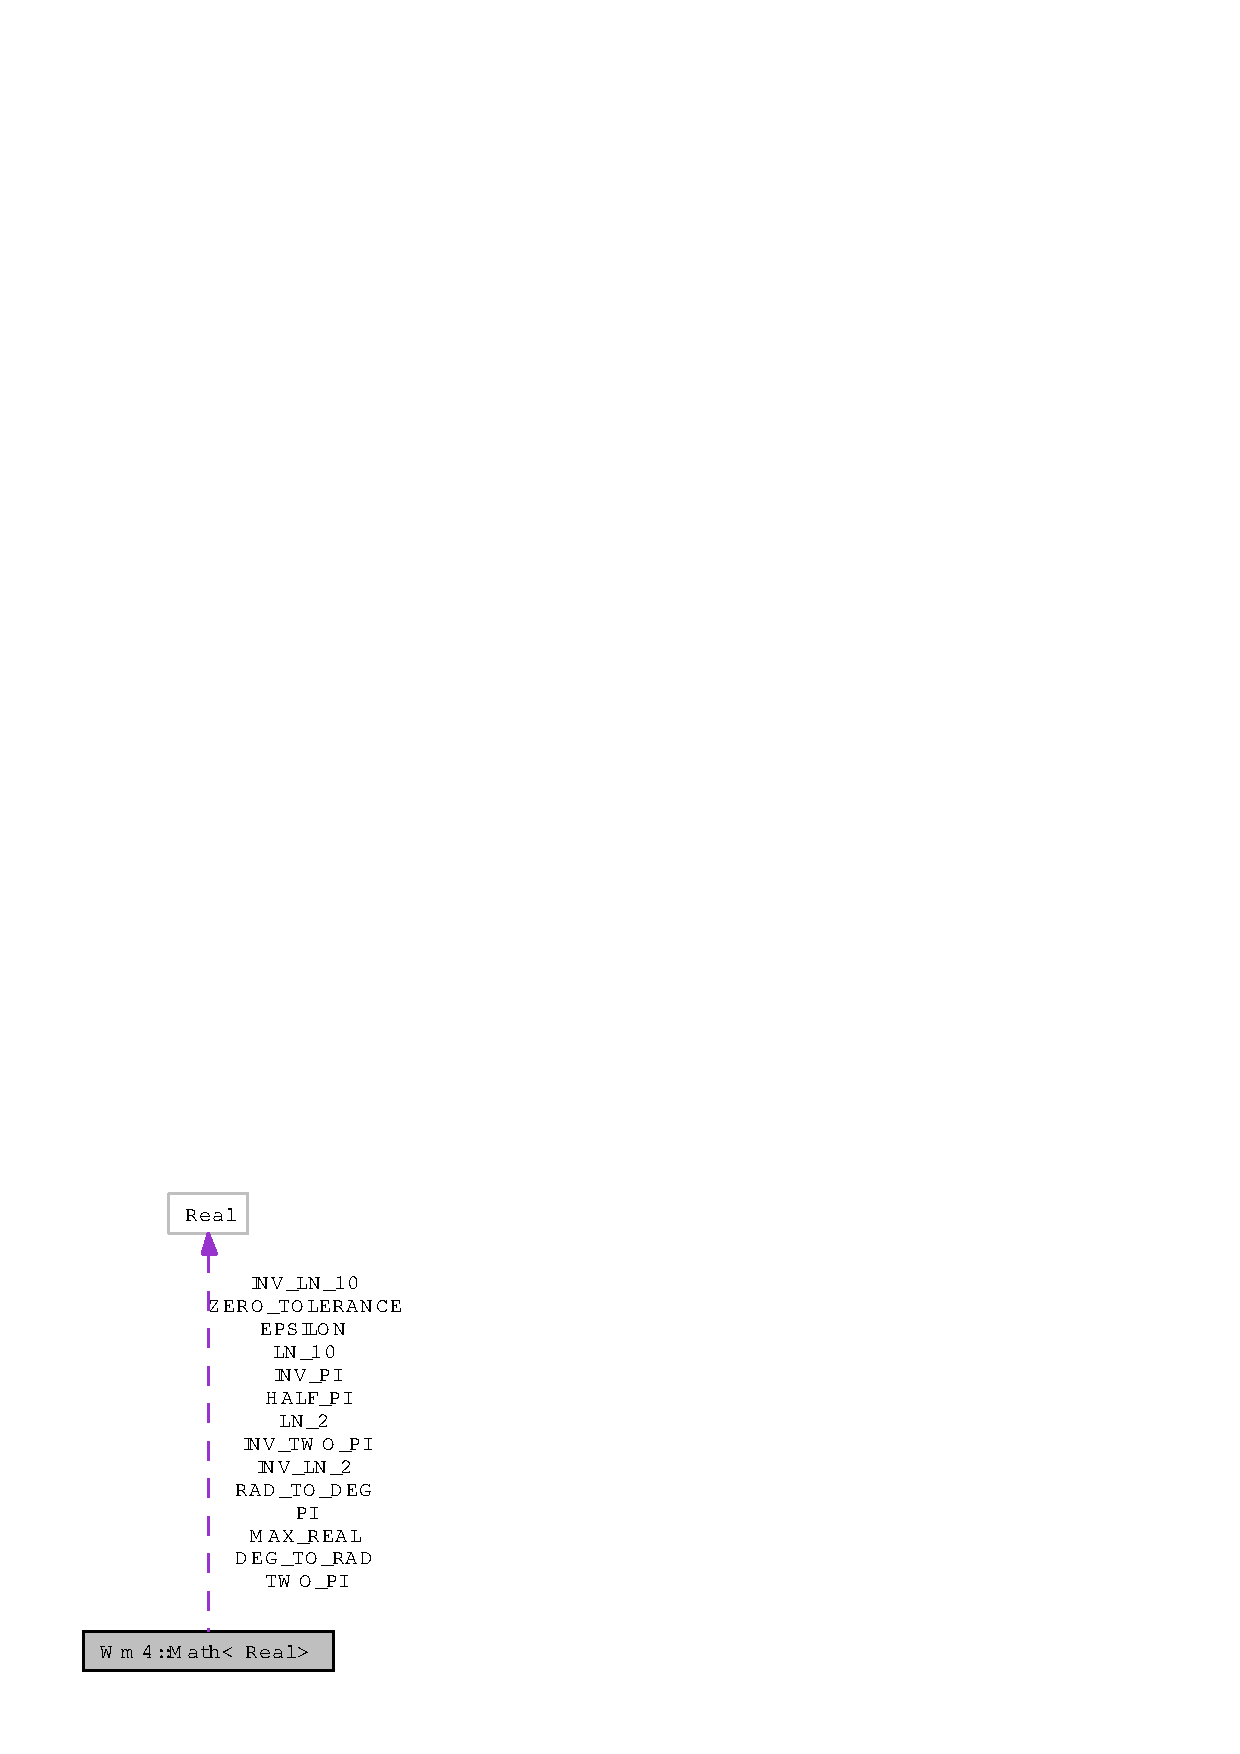
\includegraphics[width=99pt]{classWm4_1_1Math__coll__graph}
\end{center}
\end{figure}
\subsection*{Public Member Functions}
\begin{CompactItemize}
\item 
template$<$$>$ float {\bf Fast\-Inv\-Sqrt} (float f\-Value)
\item 
template$<$$>$ double {\bf Fast\-Inv\-Sqrt} (double d\-Value)
\end{CompactItemize}
\subsection*{Static Public Member Functions}
\begin{CompactItemize}
\item 
static Real {\bf ACos} (Real f\-Value)
\item 
static Real {\bf ASin} (Real f\-Value)
\item 
static Real {\bf ATan} (Real f\-Value)
\item 
static Real {\bf ATan2} (Real f\-Y, Real f\-X)
\item 
static Real {\bf Ceil} (Real f\-Value)
\item 
static Real {\bf Cos} (Real f\-Value)
\item 
static Real {\bf Exp} (Real f\-Value)
\item 
static Real {\bf FAbs} (Real f\-Value)
\item 
static Real {\bf Floor} (Real f\-Value)
\item 
static Real {\bf FMod} (Real f\-X, Real f\-Y)
\item 
static Real {\bf Inv\-Sqrt} (Real f\-Value)
\item 
static Real {\bf Log} (Real f\-Value)
\item 
static Real {\bf Log2} (Real f\-Value)
\item 
static Real {\bf Log10} (Real f\-Value)
\item 
static Real {\bf Pow} (Real f\-Base, Real f\-Exponent)
\item 
static Real {\bf Sin} (Real f\-Value)
\item 
static Real {\bf Sqr} (Real f\-Value)
\item 
static Real {\bf Sqrt} (Real f\-Value)
\item 
static Real {\bf Tan} (Real f\-Value)
\item 
static int {\bf Sign} (int i\-Value)
\item 
static Real {\bf Sign} (Real f\-Value)
\item 
static Real {\bf Unit\-Random} (unsigned int ui\-Seed=0)
\item 
static Real {\bf Symmetric\-Random} (unsigned int ui\-Seed=0)
\item 
static Real {\bf Interval\-Random} (Real f\-Min, Real f\-Max, unsigned int ui\-Seed=0)
\item 
static Real {\bf Fast\-Sin0} (Real f\-Angle)
\item 
static Real {\bf Fast\-Sin1} (Real f\-Angle)
\item 
static Real {\bf Fast\-Cos0} (Real f\-Angle)
\item 
static Real {\bf Fast\-Cos1} (Real f\-Angle)
\item 
static Real {\bf Fast\-Tan0} (Real f\-Angle)
\item 
static Real {\bf Fast\-Tan1} (Real f\-Angle)
\item 
static Real {\bf Fast\-Inv\-Sin0} (Real f\-Value)
\item 
static Real {\bf Fast\-Inv\-Sin1} (Real f\-Value)
\item 
static Real {\bf Fast\-Inv\-Cos0} (Real f\-Value)
\item 
static Real {\bf Fast\-Inv\-Cos1} (Real f\-Value)
\item 
static Real {\bf Fast\-Inv\-Tan0} (Real f\-Value)
\item 
static Real {\bf Fast\-Inv\-Tan1} (Real f\-Value)
\item 
static Real {\bf Fast\-Inv\-Sqrt} (Real f\-Value)
\item 
static Real {\bf Fast\-Neg\-Exp0} (Real f\-Value)
\item 
static Real {\bf Fast\-Neg\-Exp1} (Real f\-Value)
\item 
static Real {\bf Fast\-Neg\-Exp2} (Real f\-Value)
\item 
static Real {\bf Fast\-Neg\-Exp3} (Real f\-Value)
\end{CompactItemize}
\subsection*{Static Public Attributes}
\begin{CompactItemize}
\item 
static WM4\_\-FOUNDATION\_\-ITEM const Real {\bf EPSILON}
\item 
static WM4\_\-FOUNDATION\_\-ITEM const Real {\bf ZERO\_\-TOLERANCE}
\item 
static WM4\_\-FOUNDATION\_\-ITEM const Real {\bf MAX\_\-REAL}
\item 
static WM4\_\-FOUNDATION\_\-ITEM const Real {\bf PI}
\item 
static WM4\_\-FOUNDATION\_\-ITEM const Real {\bf TWO\_\-PI}
\item 
static WM4\_\-FOUNDATION\_\-ITEM const Real {\bf HALF\_\-PI}
\item 
static WM4\_\-FOUNDATION\_\-ITEM const Real {\bf INV\_\-PI}
\item 
static WM4\_\-FOUNDATION\_\-ITEM const Real {\bf INV\_\-TWO\_\-PI}
\item 
static WM4\_\-FOUNDATION\_\-ITEM const Real {\bf DEG\_\-TO\_\-RAD}
\item 
static WM4\_\-FOUNDATION\_\-ITEM const Real {\bf RAD\_\-TO\_\-DEG}
\item 
static WM4\_\-FOUNDATION\_\-ITEM const Real {\bf LN\_\-2}
\item 
static WM4\_\-FOUNDATION\_\-ITEM const Real {\bf LN\_\-10}
\item 
static WM4\_\-FOUNDATION\_\-ITEM const Real {\bf INV\_\-LN\_\-2}
\item 
static WM4\_\-FOUNDATION\_\-ITEM const Real {\bf INV\_\-LN\_\-10}
\end{CompactItemize}
\subsubsection*{template$<$class Real$>$ class Wm4::Math$<$ Real $>$}



\subsection{Member Function Documentation}
\index{Wm4::Math@{Wm4::Math}!ACos@{ACos}}
\index{ACos@{ACos}!Wm4::Math@{Wm4::Math}}
\subsubsection{\setlength{\rightskip}{0pt plus 5cm}template$<$class Real$>$ Real {\bf Wm4::Math}$<$ Real $>$::ACos (Real {\em f\-Value})\hspace{0.3cm}{\tt  [static]}}\label{classWm4_1_1Math_5a99eeb1bbcc52532f7512b596f46fee}


\index{Wm4::Math@{Wm4::Math}!ASin@{ASin}}
\index{ASin@{ASin}!Wm4::Math@{Wm4::Math}}
\subsubsection{\setlength{\rightskip}{0pt plus 5cm}template$<$class Real$>$ Real {\bf Wm4::Math}$<$ Real $>$::ASin (Real {\em f\-Value})\hspace{0.3cm}{\tt  [static]}}\label{classWm4_1_1Math_f0cc4c16dcefcf9535405cef650eab79}


\index{Wm4::Math@{Wm4::Math}!ATan@{ATan}}
\index{ATan@{ATan}!Wm4::Math@{Wm4::Math}}
\subsubsection{\setlength{\rightskip}{0pt plus 5cm}template$<$class Real$>$ Real {\bf Wm4::Math}$<$ Real $>$::ATan (Real {\em f\-Value})\hspace{0.3cm}{\tt  [static]}}\label{classWm4_1_1Math_d8797e64583fc1536d14460d4aa5a35d}


\index{Wm4::Math@{Wm4::Math}!ATan2@{ATan2}}
\index{ATan2@{ATan2}!Wm4::Math@{Wm4::Math}}
\subsubsection{\setlength{\rightskip}{0pt plus 5cm}template$<$class Real$>$ Real {\bf Wm4::Math}$<$ Real $>$::ATan2 (Real {\em f\-Y}, Real {\em f\-X})\hspace{0.3cm}{\tt  [static]}}\label{classWm4_1_1Math_12ff5ddc580d5a69f291ee9901242b8b}


\index{Wm4::Math@{Wm4::Math}!Ceil@{Ceil}}
\index{Ceil@{Ceil}!Wm4::Math@{Wm4::Math}}
\subsubsection{\setlength{\rightskip}{0pt plus 5cm}template$<$class Real$>$ Real {\bf Wm4::Math}$<$ Real $>$::Ceil (Real {\em f\-Value})\hspace{0.3cm}{\tt  [static]}}\label{classWm4_1_1Math_3fb661e8ea601da33bd46a8c442bfe42}


\index{Wm4::Math@{Wm4::Math}!Cos@{Cos}}
\index{Cos@{Cos}!Wm4::Math@{Wm4::Math}}
\subsubsection{\setlength{\rightskip}{0pt plus 5cm}template$<$class Real$>$ Real {\bf Wm4::Math}$<$ Real $>$::Cos (Real {\em f\-Value})\hspace{0.3cm}{\tt  [static]}}\label{classWm4_1_1Math_fd6959dae9326beb85a9aa63715abe22}


\index{Wm4::Math@{Wm4::Math}!Exp@{Exp}}
\index{Exp@{Exp}!Wm4::Math@{Wm4::Math}}
\subsubsection{\setlength{\rightskip}{0pt plus 5cm}template$<$class Real$>$ Real {\bf Wm4::Math}$<$ Real $>$::Exp (Real {\em f\-Value})\hspace{0.3cm}{\tt  [static]}}\label{classWm4_1_1Math_6fe0f8b629d9101caf4f0048af3723be}


\index{Wm4::Math@{Wm4::Math}!FAbs@{FAbs}}
\index{FAbs@{FAbs}!Wm4::Math@{Wm4::Math}}
\subsubsection{\setlength{\rightskip}{0pt plus 5cm}template$<$class Real$>$ Real {\bf Wm4::Math}$<$ Real $>$::FAbs (Real {\em f\-Value})\hspace{0.3cm}{\tt  [static]}}\label{classWm4_1_1Math_4d05439576b1f7a51883e93ca5da8841}


\index{Wm4::Math@{Wm4::Math}!Floor@{Floor}}
\index{Floor@{Floor}!Wm4::Math@{Wm4::Math}}
\subsubsection{\setlength{\rightskip}{0pt plus 5cm}template$<$class Real$>$ Real {\bf Wm4::Math}$<$ Real $>$::Floor (Real {\em f\-Value})\hspace{0.3cm}{\tt  [static]}}\label{classWm4_1_1Math_8effc599055e9a3ddd6d51e8ab2f6ea7}


\index{Wm4::Math@{Wm4::Math}!FMod@{FMod}}
\index{FMod@{FMod}!Wm4::Math@{Wm4::Math}}
\subsubsection{\setlength{\rightskip}{0pt plus 5cm}template$<$class Real$>$ Real {\bf Wm4::Math}$<$ Real $>$::FMod (Real {\em f\-X}, Real {\em f\-Y})\hspace{0.3cm}{\tt  [static]}}\label{classWm4_1_1Math_e5a1db646c275f72a75cb62173c64d15}


\index{Wm4::Math@{Wm4::Math}!InvSqrt@{InvSqrt}}
\index{InvSqrt@{InvSqrt}!Wm4::Math@{Wm4::Math}}
\subsubsection{\setlength{\rightskip}{0pt plus 5cm}template$<$class Real$>$ Real {\bf Wm4::Math}$<$ Real $>$::Inv\-Sqrt (Real {\em f\-Value})\hspace{0.3cm}{\tt  [static]}}\label{classWm4_1_1Math_3f72786907e61979bf643d93c78a6897}


\index{Wm4::Math@{Wm4::Math}!Log@{Log}}
\index{Log@{Log}!Wm4::Math@{Wm4::Math}}
\subsubsection{\setlength{\rightskip}{0pt plus 5cm}template$<$class Real$>$ Real {\bf Wm4::Math}$<$ Real $>$::{\bf Log} (Real {\em f\-Value})\hspace{0.3cm}{\tt  [static]}}\label{classWm4_1_1Math_c57ffd80f97eba8d7f69bbf546488fce}


\index{Wm4::Math@{Wm4::Math}!Log2@{Log2}}
\index{Log2@{Log2}!Wm4::Math@{Wm4::Math}}
\subsubsection{\setlength{\rightskip}{0pt plus 5cm}template$<$class Real$>$ Real {\bf Wm4::Math}$<$ Real $>$::Log2 (Real {\em f\-Value})\hspace{0.3cm}{\tt  [static]}}\label{classWm4_1_1Math_3dca722bc6b3252f8911c5a5f5c6d9fd}


\index{Wm4::Math@{Wm4::Math}!Log10@{Log10}}
\index{Log10@{Log10}!Wm4::Math@{Wm4::Math}}
\subsubsection{\setlength{\rightskip}{0pt plus 5cm}template$<$class Real$>$ Real {\bf Wm4::Math}$<$ Real $>$::Log10 (Real {\em f\-Value})\hspace{0.3cm}{\tt  [static]}}\label{classWm4_1_1Math_cf4b54b6f3dccd9d8a14afd5e65cb003}


\index{Wm4::Math@{Wm4::Math}!Pow@{Pow}}
\index{Pow@{Pow}!Wm4::Math@{Wm4::Math}}
\subsubsection{\setlength{\rightskip}{0pt plus 5cm}template$<$class Real$>$ Real {\bf Wm4::Math}$<$ Real $>$::Pow (Real {\em f\-Base}, Real {\em f\-Exponent})\hspace{0.3cm}{\tt  [static]}}\label{classWm4_1_1Math_fdce58a0449eacd2eb637d8ff77bb02c}


\index{Wm4::Math@{Wm4::Math}!Sin@{Sin}}
\index{Sin@{Sin}!Wm4::Math@{Wm4::Math}}
\subsubsection{\setlength{\rightskip}{0pt plus 5cm}template$<$class Real$>$ Real {\bf Wm4::Math}$<$ Real $>$::Sin (Real {\em f\-Value})\hspace{0.3cm}{\tt  [static]}}\label{classWm4_1_1Math_4840a7be35d06c9434c9f0b7355ef53a}


\index{Wm4::Math@{Wm4::Math}!Sqr@{Sqr}}
\index{Sqr@{Sqr}!Wm4::Math@{Wm4::Math}}
\subsubsection{\setlength{\rightskip}{0pt plus 5cm}template$<$class Real$>$ Real {\bf Wm4::Math}$<$ Real $>$::Sqr (Real {\em f\-Value})\hspace{0.3cm}{\tt  [static]}}\label{classWm4_1_1Math_c5800eb19a5392fadc476e42b9a5b8a4}


\index{Wm4::Math@{Wm4::Math}!Sqrt@{Sqrt}}
\index{Sqrt@{Sqrt}!Wm4::Math@{Wm4::Math}}
\subsubsection{\setlength{\rightskip}{0pt plus 5cm}template$<$class Real$>$ Real {\bf Wm4::Math}$<$ Real $>$::Sqrt (Real {\em f\-Value})\hspace{0.3cm}{\tt  [static]}}\label{classWm4_1_1Math_682df77a16fb68959c657ef2889b4797}


\index{Wm4::Math@{Wm4::Math}!Tan@{Tan}}
\index{Tan@{Tan}!Wm4::Math@{Wm4::Math}}
\subsubsection{\setlength{\rightskip}{0pt plus 5cm}template$<$class Real$>$ Real {\bf Wm4::Math}$<$ Real $>$::Tan (Real {\em f\-Value})\hspace{0.3cm}{\tt  [static]}}\label{classWm4_1_1Math_11b14bcbcb1683b01521e98e93c8b5fc}


\index{Wm4::Math@{Wm4::Math}!Sign@{Sign}}
\index{Sign@{Sign}!Wm4::Math@{Wm4::Math}}
\subsubsection{\setlength{\rightskip}{0pt plus 5cm}template$<$class Real$>$ int {\bf Wm4::Math}$<$ Real $>$::Sign (int {\em i\-Value})\hspace{0.3cm}{\tt  [static]}}\label{classWm4_1_1Math_2fb693eb53ba1b2643305c8f50b0d747}


\index{Wm4::Math@{Wm4::Math}!Sign@{Sign}}
\index{Sign@{Sign}!Wm4::Math@{Wm4::Math}}
\subsubsection{\setlength{\rightskip}{0pt plus 5cm}template$<$class Real$>$ Real {\bf Wm4::Math}$<$ Real $>$::Sign (Real {\em f\-Value})\hspace{0.3cm}{\tt  [static]}}\label{classWm4_1_1Math_1c85feb0b08de9215a49a6e1c34504ff}


\index{Wm4::Math@{Wm4::Math}!UnitRandom@{UnitRandom}}
\index{UnitRandom@{UnitRandom}!Wm4::Math@{Wm4::Math}}
\subsubsection{\setlength{\rightskip}{0pt plus 5cm}template$<$class Real$>$ Real {\bf Wm4::Math}$<$ Real $>$::Unit\-Random (unsigned int {\em ui\-Seed} = {\tt 0})\hspace{0.3cm}{\tt  [static]}}\label{classWm4_1_1Math_87baf2aa4f385477216614d478d99a43}


\index{Wm4::Math@{Wm4::Math}!SymmetricRandom@{SymmetricRandom}}
\index{SymmetricRandom@{SymmetricRandom}!Wm4::Math@{Wm4::Math}}
\subsubsection{\setlength{\rightskip}{0pt plus 5cm}template$<$class Real$>$ Real {\bf Wm4::Math}$<$ Real $>$::Symmetric\-Random (unsigned int {\em ui\-Seed} = {\tt 0})\hspace{0.3cm}{\tt  [static]}}\label{classWm4_1_1Math_3ccd8e5bce7153bf90e85c21cd943d9e}


\index{Wm4::Math@{Wm4::Math}!IntervalRandom@{IntervalRandom}}
\index{IntervalRandom@{IntervalRandom}!Wm4::Math@{Wm4::Math}}
\subsubsection{\setlength{\rightskip}{0pt plus 5cm}template$<$class Real$>$ Real {\bf Wm4::Math}$<$ Real $>$::Interval\-Random (Real {\em f\-Min}, Real {\em f\-Max}, unsigned int {\em ui\-Seed} = {\tt 0})\hspace{0.3cm}{\tt  [static]}}\label{classWm4_1_1Math_15447b36fcec0d09a39691e17878c9af}


\index{Wm4::Math@{Wm4::Math}!FastSin0@{FastSin0}}
\index{FastSin0@{FastSin0}!Wm4::Math@{Wm4::Math}}
\subsubsection{\setlength{\rightskip}{0pt plus 5cm}template$<$class Real$>$ Real {\bf Wm4::Math}$<$ Real $>$::Fast\-Sin0 (Real {\em f\-Angle})\hspace{0.3cm}{\tt  [static]}}\label{classWm4_1_1Math_c4119128bbb06bc1ccb037c3d91d952d}


\index{Wm4::Math@{Wm4::Math}!FastSin1@{FastSin1}}
\index{FastSin1@{FastSin1}!Wm4::Math@{Wm4::Math}}
\subsubsection{\setlength{\rightskip}{0pt plus 5cm}template$<$class Real$>$ Real {\bf Wm4::Math}$<$ Real $>$::Fast\-Sin1 (Real {\em f\-Angle})\hspace{0.3cm}{\tt  [static]}}\label{classWm4_1_1Math_e0f8fd007f571ca397e4e4f2486d968c}


\index{Wm4::Math@{Wm4::Math}!FastCos0@{FastCos0}}
\index{FastCos0@{FastCos0}!Wm4::Math@{Wm4::Math}}
\subsubsection{\setlength{\rightskip}{0pt plus 5cm}template$<$class Real$>$ Real {\bf Wm4::Math}$<$ Real $>$::Fast\-Cos0 (Real {\em f\-Angle})\hspace{0.3cm}{\tt  [static]}}\label{classWm4_1_1Math_c7a657948c6ac9d198105c9eccaedb86}


\index{Wm4::Math@{Wm4::Math}!FastCos1@{FastCos1}}
\index{FastCos1@{FastCos1}!Wm4::Math@{Wm4::Math}}
\subsubsection{\setlength{\rightskip}{0pt plus 5cm}template$<$class Real$>$ Real {\bf Wm4::Math}$<$ Real $>$::Fast\-Cos1 (Real {\em f\-Angle})\hspace{0.3cm}{\tt  [static]}}\label{classWm4_1_1Math_f4fdc4f15c2ded283b94494e08db6fc4}


\index{Wm4::Math@{Wm4::Math}!FastTan0@{FastTan0}}
\index{FastTan0@{FastTan0}!Wm4::Math@{Wm4::Math}}
\subsubsection{\setlength{\rightskip}{0pt plus 5cm}template$<$class Real$>$ Real {\bf Wm4::Math}$<$ Real $>$::Fast\-Tan0 (Real {\em f\-Angle})\hspace{0.3cm}{\tt  [static]}}\label{classWm4_1_1Math_7d94c326871ff1aa03e2e839b67adc21}


\index{Wm4::Math@{Wm4::Math}!FastTan1@{FastTan1}}
\index{FastTan1@{FastTan1}!Wm4::Math@{Wm4::Math}}
\subsubsection{\setlength{\rightskip}{0pt plus 5cm}template$<$class Real$>$ Real {\bf Wm4::Math}$<$ Real $>$::Fast\-Tan1 (Real {\em f\-Angle})\hspace{0.3cm}{\tt  [static]}}\label{classWm4_1_1Math_ae6316c29815e109aeb9194773811789}


\index{Wm4::Math@{Wm4::Math}!FastInvSin0@{FastInvSin0}}
\index{FastInvSin0@{FastInvSin0}!Wm4::Math@{Wm4::Math}}
\subsubsection{\setlength{\rightskip}{0pt plus 5cm}template$<$class Real$>$ Real {\bf Wm4::Math}$<$ Real $>$::Fast\-Inv\-Sin0 (Real {\em f\-Value})\hspace{0.3cm}{\tt  [static]}}\label{classWm4_1_1Math_f2b501ba906fb31c3dade17977003352}


\index{Wm4::Math@{Wm4::Math}!FastInvSin1@{FastInvSin1}}
\index{FastInvSin1@{FastInvSin1}!Wm4::Math@{Wm4::Math}}
\subsubsection{\setlength{\rightskip}{0pt plus 5cm}template$<$class Real$>$ Real {\bf Wm4::Math}$<$ Real $>$::Fast\-Inv\-Sin1 (Real {\em f\-Value})\hspace{0.3cm}{\tt  [static]}}\label{classWm4_1_1Math_c5cb2393220d2670af98e35ef6f00dd5}


\index{Wm4::Math@{Wm4::Math}!FastInvCos0@{FastInvCos0}}
\index{FastInvCos0@{FastInvCos0}!Wm4::Math@{Wm4::Math}}
\subsubsection{\setlength{\rightskip}{0pt plus 5cm}template$<$class Real$>$ Real {\bf Wm4::Math}$<$ Real $>$::Fast\-Inv\-Cos0 (Real {\em f\-Value})\hspace{0.3cm}{\tt  [static]}}\label{classWm4_1_1Math_32a199184eb80a9d5375bda93d926f15}


\index{Wm4::Math@{Wm4::Math}!FastInvCos1@{FastInvCos1}}
\index{FastInvCos1@{FastInvCos1}!Wm4::Math@{Wm4::Math}}
\subsubsection{\setlength{\rightskip}{0pt plus 5cm}template$<$class Real$>$ Real {\bf Wm4::Math}$<$ Real $>$::Fast\-Inv\-Cos1 (Real {\em f\-Value})\hspace{0.3cm}{\tt  [static]}}\label{classWm4_1_1Math_3f7614e98c6c9f5bd7d2b69fcb5584a1}


\index{Wm4::Math@{Wm4::Math}!FastInvTan0@{FastInvTan0}}
\index{FastInvTan0@{FastInvTan0}!Wm4::Math@{Wm4::Math}}
\subsubsection{\setlength{\rightskip}{0pt plus 5cm}template$<$class Real$>$ Real {\bf Wm4::Math}$<$ Real $>$::Fast\-Inv\-Tan0 (Real {\em f\-Value})\hspace{0.3cm}{\tt  [static]}}\label{classWm4_1_1Math_f71b8efef9741a01ead8958f15030396}


\index{Wm4::Math@{Wm4::Math}!FastInvTan1@{FastInvTan1}}
\index{FastInvTan1@{FastInvTan1}!Wm4::Math@{Wm4::Math}}
\subsubsection{\setlength{\rightskip}{0pt plus 5cm}template$<$class Real$>$ Real {\bf Wm4::Math}$<$ Real $>$::Fast\-Inv\-Tan1 (Real {\em f\-Value})\hspace{0.3cm}{\tt  [static]}}\label{classWm4_1_1Math_6a4efcdad00d630ff4397e77dab1e74a}


\index{Wm4::Math@{Wm4::Math}!FastInvSqrt@{FastInvSqrt}}
\index{FastInvSqrt@{FastInvSqrt}!Wm4::Math@{Wm4::Math}}
\subsubsection{\setlength{\rightskip}{0pt plus 5cm}template$<$class Real$>$ static Real {\bf Wm4::Math}$<$ Real $>$::Fast\-Inv\-Sqrt (Real {\em f\-Value})\hspace{0.3cm}{\tt  [static]}}\label{classWm4_1_1Math_b8972caffea9b5925f5a4ee6026c7d51}


\index{Wm4::Math@{Wm4::Math}!FastNegExp0@{FastNegExp0}}
\index{FastNegExp0@{FastNegExp0}!Wm4::Math@{Wm4::Math}}
\subsubsection{\setlength{\rightskip}{0pt plus 5cm}template$<$class Real$>$ Real {\bf Wm4::Math}$<$ Real $>$::Fast\-Neg\-Exp0 (Real {\em f\-Value})\hspace{0.3cm}{\tt  [static]}}\label{classWm4_1_1Math_050ac5217709e69b7a60b360e7fa377a}


\index{Wm4::Math@{Wm4::Math}!FastNegExp1@{FastNegExp1}}
\index{FastNegExp1@{FastNegExp1}!Wm4::Math@{Wm4::Math}}
\subsubsection{\setlength{\rightskip}{0pt plus 5cm}template$<$class Real$>$ Real {\bf Wm4::Math}$<$ Real $>$::Fast\-Neg\-Exp1 (Real {\em f\-Value})\hspace{0.3cm}{\tt  [static]}}\label{classWm4_1_1Math_03ca49eb8afa870d5ef49c85e8fb0894}


\index{Wm4::Math@{Wm4::Math}!FastNegExp2@{FastNegExp2}}
\index{FastNegExp2@{FastNegExp2}!Wm4::Math@{Wm4::Math}}
\subsubsection{\setlength{\rightskip}{0pt plus 5cm}template$<$class Real$>$ Real {\bf Wm4::Math}$<$ Real $>$::Fast\-Neg\-Exp2 (Real {\em f\-Value})\hspace{0.3cm}{\tt  [static]}}\label{classWm4_1_1Math_49a93e80e6fb29e6bdfd2a818e5d10cd}


\index{Wm4::Math@{Wm4::Math}!FastNegExp3@{FastNegExp3}}
\index{FastNegExp3@{FastNegExp3}!Wm4::Math@{Wm4::Math}}
\subsubsection{\setlength{\rightskip}{0pt plus 5cm}template$<$class Real$>$ Real {\bf Wm4::Math}$<$ Real $>$::Fast\-Neg\-Exp3 (Real {\em f\-Value})\hspace{0.3cm}{\tt  [static]}}\label{classWm4_1_1Math_0ddf42e768ea9d977ea76d37c8b71021}


\index{Wm4::Math@{Wm4::Math}!FastInvSqrt@{FastInvSqrt}}
\index{FastInvSqrt@{FastInvSqrt}!Wm4::Math@{Wm4::Math}}
\subsubsection{\setlength{\rightskip}{0pt plus 5cm}template$<$$>$ float {\bf Wm4::Math}$<$ float $>$::Fast\-Inv\-Sqrt (float {\em f\-Value})}\label{classWm4_1_1Math_87d88d16bb3909384320b2b7b89c25de}


\index{Wm4::Math@{Wm4::Math}!FastInvSqrt@{FastInvSqrt}}
\index{FastInvSqrt@{FastInvSqrt}!Wm4::Math@{Wm4::Math}}
\subsubsection{\setlength{\rightskip}{0pt plus 5cm}template$<$$>$ double {\bf Wm4::Math}$<$ double $>$::Fast\-Inv\-Sqrt (double {\em d\-Value})}\label{classWm4_1_1Math_6ef8a7a052083195e74864c9d3c64268}




\subsection{Member Data Documentation}
\index{Wm4::Math@{Wm4::Math}!EPSILON@{EPSILON}}
\index{EPSILON@{EPSILON}!Wm4::Math@{Wm4::Math}}
\subsubsection{\setlength{\rightskip}{0pt plus 5cm}template$<$class Real$>$ WM4\_\-FOUNDATION\_\-ITEM const Real {\bf Wm4::Math}$<$ Real $>$::{\bf EPSILON}\hspace{0.3cm}{\tt  [static]}}\label{classWm4_1_1Math_862e7780520f49ef23bb9062b0c5ca8f}


\index{Wm4::Math@{Wm4::Math}!ZERO_TOLERANCE@{ZERO\_\-TOLERANCE}}
\index{ZERO_TOLERANCE@{ZERO\_\-TOLERANCE}!Wm4::Math@{Wm4::Math}}
\subsubsection{\setlength{\rightskip}{0pt plus 5cm}template$<$class Real$>$ WM4\_\-FOUNDATION\_\-ITEM const Real {\bf Wm4::Math}$<$ Real $>$::{\bf ZERO\_\-TOLERANCE}\hspace{0.3cm}{\tt  [static]}}\label{classWm4_1_1Math_16c4a22ba9c410abf60185cf082b2951}


\index{Wm4::Math@{Wm4::Math}!MAX_REAL@{MAX\_\-REAL}}
\index{MAX_REAL@{MAX\_\-REAL}!Wm4::Math@{Wm4::Math}}
\subsubsection{\setlength{\rightskip}{0pt plus 5cm}template$<$class Real$>$ WM4\_\-FOUNDATION\_\-ITEM const Real {\bf Wm4::Math}$<$ Real $>$::{\bf MAX\_\-REAL}\hspace{0.3cm}{\tt  [static]}}\label{classWm4_1_1Math_de032b84b480b45e883e1d65db857a55}


\index{Wm4::Math@{Wm4::Math}!PI@{PI}}
\index{PI@{PI}!Wm4::Math@{Wm4::Math}}
\subsubsection{\setlength{\rightskip}{0pt plus 5cm}template$<$class Real$>$ WM4\_\-FOUNDATION\_\-ITEM const Real {\bf Wm4::Math}$<$ Real $>$::{\bf PI}\hspace{0.3cm}{\tt  [static]}}\label{classWm4_1_1Math_41ed76ae25a067e71c45f3e96bee186b}


\index{Wm4::Math@{Wm4::Math}!TWO_PI@{TWO\_\-PI}}
\index{TWO_PI@{TWO\_\-PI}!Wm4::Math@{Wm4::Math}}
\subsubsection{\setlength{\rightskip}{0pt plus 5cm}template$<$class Real$>$ WM4\_\-FOUNDATION\_\-ITEM const Real {\bf Wm4::Math}$<$ Real $>$::{\bf TWO\_\-PI}\hspace{0.3cm}{\tt  [static]}}\label{classWm4_1_1Math_cc5062f3c348ccb4e2f16bcf75ea5ddb}


\index{Wm4::Math@{Wm4::Math}!HALF_PI@{HALF\_\-PI}}
\index{HALF_PI@{HALF\_\-PI}!Wm4::Math@{Wm4::Math}}
\subsubsection{\setlength{\rightskip}{0pt plus 5cm}template$<$class Real$>$ WM4\_\-FOUNDATION\_\-ITEM const Real {\bf Wm4::Math}$<$ Real $>$::{\bf HALF\_\-PI}\hspace{0.3cm}{\tt  [static]}}\label{classWm4_1_1Math_70a1d1c090a188ce377e3093a265c40b}


\index{Wm4::Math@{Wm4::Math}!INV_PI@{INV\_\-PI}}
\index{INV_PI@{INV\_\-PI}!Wm4::Math@{Wm4::Math}}
\subsubsection{\setlength{\rightskip}{0pt plus 5cm}template$<$class Real$>$ WM4\_\-FOUNDATION\_\-ITEM const Real {\bf Wm4::Math}$<$ Real $>$::{\bf INV\_\-PI}\hspace{0.3cm}{\tt  [static]}}\label{classWm4_1_1Math_2c506a14173cd91d324a5eb12a819b80}


\index{Wm4::Math@{Wm4::Math}!INV_TWO_PI@{INV\_\-TWO\_\-PI}}
\index{INV_TWO_PI@{INV\_\-TWO\_\-PI}!Wm4::Math@{Wm4::Math}}
\subsubsection{\setlength{\rightskip}{0pt plus 5cm}template$<$class Real$>$ WM4\_\-FOUNDATION\_\-ITEM const Real {\bf Wm4::Math}$<$ Real $>$::{\bf INV\_\-TWO\_\-PI}\hspace{0.3cm}{\tt  [static]}}\label{classWm4_1_1Math_b807bb61cbc044afcebcf4c6e2e2cedb}


\index{Wm4::Math@{Wm4::Math}!DEG_TO_RAD@{DEG\_\-TO\_\-RAD}}
\index{DEG_TO_RAD@{DEG\_\-TO\_\-RAD}!Wm4::Math@{Wm4::Math}}
\subsubsection{\setlength{\rightskip}{0pt plus 5cm}template$<$class Real$>$ WM4\_\-FOUNDATION\_\-ITEM const Real {\bf Wm4::Math}$<$ Real $>$::{\bf DEG\_\-TO\_\-RAD}\hspace{0.3cm}{\tt  [static]}}\label{classWm4_1_1Math_0c9949da37870540982e2544895479c6}


\index{Wm4::Math@{Wm4::Math}!RAD_TO_DEG@{RAD\_\-TO\_\-DEG}}
\index{RAD_TO_DEG@{RAD\_\-TO\_\-DEG}!Wm4::Math@{Wm4::Math}}
\subsubsection{\setlength{\rightskip}{0pt plus 5cm}template$<$class Real$>$ WM4\_\-FOUNDATION\_\-ITEM const Real {\bf Wm4::Math}$<$ Real $>$::{\bf RAD\_\-TO\_\-DEG}\hspace{0.3cm}{\tt  [static]}}\label{classWm4_1_1Math_867d68abb2b53e14860b7889be367572}


\index{Wm4::Math@{Wm4::Math}!LN_2@{LN\_\-2}}
\index{LN_2@{LN\_\-2}!Wm4::Math@{Wm4::Math}}
\subsubsection{\setlength{\rightskip}{0pt plus 5cm}template$<$class Real$>$ WM4\_\-FOUNDATION\_\-ITEM const Real {\bf Wm4::Math}$<$ Real $>$::{\bf LN\_\-2}\hspace{0.3cm}{\tt  [static]}}\label{classWm4_1_1Math_7809361231a77d0fdb874c690427e3d4}


\index{Wm4::Math@{Wm4::Math}!LN_10@{LN\_\-10}}
\index{LN_10@{LN\_\-10}!Wm4::Math@{Wm4::Math}}
\subsubsection{\setlength{\rightskip}{0pt plus 5cm}template$<$class Real$>$ WM4\_\-FOUNDATION\_\-ITEM const Real {\bf Wm4::Math}$<$ Real $>$::{\bf LN\_\-10}\hspace{0.3cm}{\tt  [static]}}\label{classWm4_1_1Math_d55b067b5a62e2bbc5f3f3395225c788}


\index{Wm4::Math@{Wm4::Math}!INV_LN_2@{INV\_\-LN\_\-2}}
\index{INV_LN_2@{INV\_\-LN\_\-2}!Wm4::Math@{Wm4::Math}}
\subsubsection{\setlength{\rightskip}{0pt plus 5cm}template$<$class Real$>$ WM4\_\-FOUNDATION\_\-ITEM const Real {\bf Wm4::Math}$<$ Real $>$::{\bf INV\_\-LN\_\-2}\hspace{0.3cm}{\tt  [static]}}\label{classWm4_1_1Math_2bd9e85cc86fee05319aebe17706c932}


\index{Wm4::Math@{Wm4::Math}!INV_LN_10@{INV\_\-LN\_\-10}}
\index{INV_LN_10@{INV\_\-LN\_\-10}!Wm4::Math@{Wm4::Math}}
\subsubsection{\setlength{\rightskip}{0pt plus 5cm}template$<$class Real$>$ WM4\_\-FOUNDATION\_\-ITEM const Real {\bf Wm4::Math}$<$ Real $>$::{\bf INV\_\-LN\_\-10}\hspace{0.3cm}{\tt  [static]}}\label{classWm4_1_1Math_405239570d04875b42920e86207f0327}




The documentation for this class was generated from the following file:\begin{CompactItemize}
\item 
{\bf Wm4Math.h}\end{CompactItemize}

\section{Wm4::Matrix3$<$ Real $>$ Class Template Reference}
\label{classWm4_1_1Matrix3}\index{Wm4::Matrix3@{Wm4::Matrix3}}
{\tt \#include $<$Wm4Matrix3.h$>$}

Collaboration diagram for Wm4::Matrix3$<$ Real $>$:\begin{figure}[H]
\begin{center}
\leavevmode
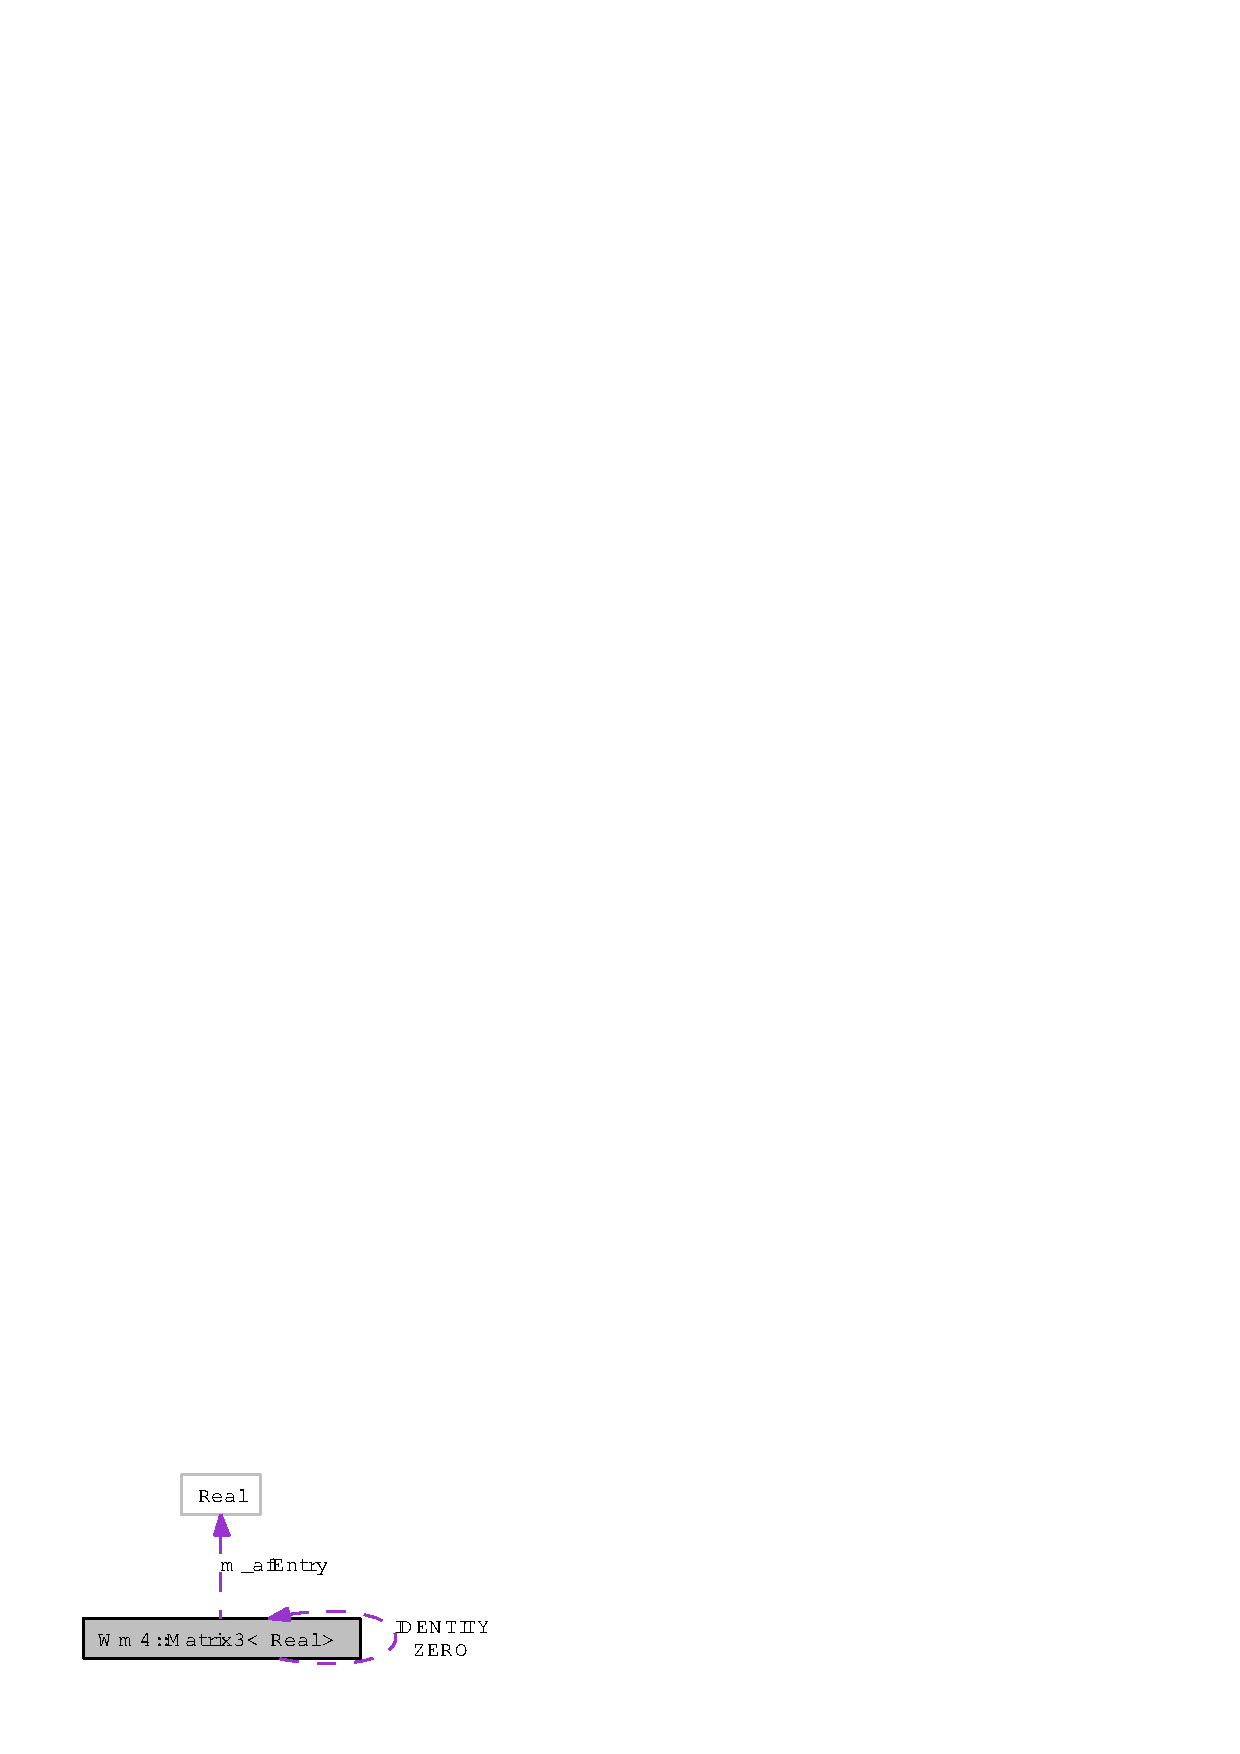
\includegraphics[width=120pt]{classWm4_1_1Matrix3__coll__graph}
\end{center}
\end{figure}
\subsection*{Public Types}
\begin{CompactItemize}
\item 
enum {\bf Euler\-Result} \{ {\bf EA\_\-UNIQUE}, 
{\bf EA\_\-NOT\_\-UNIQUE\_\-SUM}, 
{\bf EA\_\-NOT\_\-UNIQUE\_\-DIF}
 \}
\end{CompactItemize}
\subsection*{Public Member Functions}
\begin{CompactItemize}
\item 
{\bf Matrix3} (bool b\-Zero=true)
\item 
{\bf Matrix3} (const {\bf Matrix3} \&rk\-M)
\item 
{\bf Matrix3} (Real f\-M00, Real f\-M01, Real f\-M02, Real f\-M10, Real f\-M11, Real f\-M12, Real f\-M20, Real f\-M21, Real f\-M22)
\item 
{\bf Matrix3} (const Real af\-Entry[9], bool b\-Row\-Major)
\item 
{\bf Matrix3} (const {\bf Vector3}$<$ Real $>$ \&rk\-U, const {\bf Vector3}$<$ Real $>$ \&rk\-V, const {\bf Vector3}$<$ Real $>$ \&rk\-W, bool b\-Columns)
\item 
{\bf Matrix3} (const {\bf Vector3}$<$ Real $>$ $\ast$ak\-V, bool b\-Columns)
\item 
{\bf Matrix3} (Real f\-M00, Real f\-M11, Real f\-M22)
\item 
{\bf Matrix3} (const {\bf Vector3}$<$ Real $>$ \&rk\-Axis, Real f\-Angle)
\item 
{\bf Matrix3} (const {\bf Vector3}$<$ Real $>$ \&rk\-U, const {\bf Vector3}$<$ Real $>$ \&rk\-V)
\item 
{\bf Matrix3} \& {\bf Make\-Zero} ()
\item 
{\bf Matrix3} \& {\bf Make\-Identity} ()
\item 
{\bf Matrix3} \& {\bf Make\-Diagonal} (Real f\-M00, Real f\-M11, Real f\-M22)
\item 
{\bf Matrix3} \& {\bf From\-Axis\-Angle} (const {\bf Vector3}$<$ Real $>$ \&rk\-Axis, Real f\-Angle)
\item 
{\bf Matrix3} \& {\bf Make\-Tensor\-Product} (const {\bf Vector3}$<$ Real $>$ \&rk\-U, const {\bf Vector3}$<$ Real $>$ \&rk\-V)
\item 
{\bf operator const Real $\ast$} () const
\item 
{\bf operator Real $\ast$} ()
\item 
const Real $\ast$ {\bf operator[$\,$]} (int i\-Row) const
\item 
Real $\ast$ {\bf operator[$\,$]} (int i\-Row)
\item 
Real {\bf operator()} (int i\-Row, int i\-Col) const
\item 
Real \& {\bf operator()} (int i\-Row, int i\-Col)
\item 
void {\bf Set\-Row} (int i\-Row, const {\bf Vector3}$<$ Real $>$ \&rk\-V)
\item 
{\bf Vector3}$<$ Real $>$ {\bf Get\-Row} (int i\-Row) const
\item 
void {\bf Set\-Column} (int i\-Col, const {\bf Vector3}$<$ Real $>$ \&rk\-V)
\item 
{\bf Vector3}$<$ Real $>$ {\bf Get\-Column} (int i\-Col) const
\item 
void {\bf Get\-Column\-Major} (Real $\ast$af\-CMajor) const
\item 
{\bf Matrix3} \& {\bf operator=} (const {\bf Matrix3} \&rk\-M)
\item 
bool {\bf operator==} (const {\bf Matrix3} \&rk\-M) const
\item 
bool {\bf operator!=} (const {\bf Matrix3} \&rk\-M) const
\item 
bool {\bf operator$<$} (const {\bf Matrix3} \&rk\-M) const
\item 
bool {\bf operator$<$=} (const {\bf Matrix3} \&rk\-M) const
\item 
bool {\bf operator$>$} (const {\bf Matrix3} \&rk\-M) const
\item 
bool {\bf operator$>$=} (const {\bf Matrix3} \&rk\-M) const
\item 
{\bf Matrix3} {\bf operator+} (const {\bf Matrix3} \&rk\-M) const
\item 
{\bf Matrix3} {\bf operator-} (const {\bf Matrix3} \&rk\-M) const
\item 
{\bf Matrix3} {\bf operator $\ast$} (const {\bf Matrix3} \&rk\-M) const
\item 
{\bf Matrix3} {\bf operator $\ast$} (Real f\-Scalar) const 
\item 
{\bf Matrix3} {\bf operator/} (Real f\-Scalar) const 
\item 
{\bf Matrix3} {\bf operator-} () const
\item 
{\bf Matrix3} \& {\bf operator+=} (const {\bf Matrix3} \&rk\-M)
\item 
{\bf Matrix3} \& {\bf operator-=} (const {\bf Matrix3} \&rk\-M)
\item 
{\bf Matrix3} \& {\bf operator $\ast$=} (Real f\-Scalar)
\item 
{\bf Matrix3} \& {\bf operator/=} (Real f\-Scalar)
\item 
{\bf Vector3}$<$ Real $>$ {\bf operator $\ast$} (const {\bf Vector3}$<$ Real $>$ \&rk\-V) const
\item 
{\bf Matrix3} {\bf Transpose} () const
\item 
{\bf Matrix3} {\bf Transpose\-Times} (const {\bf Matrix3} \&rk\-M) const
\item 
{\bf Matrix3} {\bf Times\-Transpose} (const {\bf Matrix3} \&rk\-M) const
\item 
{\bf Matrix3} {\bf Inverse} () const
\item 
{\bf Matrix3} {\bf Adjoint} () const
\item 
Real {\bf Determinant} () const
\item 
Real {\bf QForm} (const {\bf Vector3}$<$ Real $>$ \&rk\-U, const {\bf Vector3}$<$ Real $>$ \&rk\-V) const
\item 
{\bf Matrix3} {\bf Times\-Diagonal} (const {\bf Vector3}$<$ Real $>$ \&rk\-Diag) const
\item 
{\bf Matrix3} {\bf Diagonal\-Times} (const {\bf Vector3}$<$ Real $>$ \&rk\-Diag) const
\item 
void {\bf To\-Axis\-Angle} ({\bf Vector3}$<$ Real $>$ \&rk\-Axis, Real \&rf\-Angle) const
\item 
void {\bf Orthonormalize} ()
\item 
void {\bf Eigen\-Decomposition} ({\bf Matrix3} \&rk\-Rot, {\bf Matrix3} \&rk\-Diag) const
\item 
{\bf Matrix3} \& {\bf From\-Euler\-Angles\-XYZ} (Real f\-XAngle, Real f\-YAngle, Real f\-ZAngle)
\item 
{\bf Matrix3} \& {\bf From\-Euler\-Angles\-XZY} (Real f\-XAngle, Real f\-ZAngle, Real f\-YAngle)
\item 
{\bf Matrix3} \& {\bf From\-Euler\-Angles\-YXZ} (Real f\-YAngle, Real f\-XAngle, Real f\-ZAngle)
\item 
{\bf Matrix3} \& {\bf From\-Euler\-Angles\-YZX} (Real f\-YAngle, Real f\-ZAngle, Real f\-XAngle)
\item 
{\bf Matrix3} \& {\bf From\-Euler\-Angles\-ZXY} (Real f\-ZAngle, Real f\-XAngle, Real f\-YAngle)
\item 
{\bf Matrix3} \& {\bf From\-Euler\-Angles\-ZYX} (Real f\-ZAngle, Real f\-YAngle, Real f\-XAngle)
\item 
{\bf Euler\-Result} {\bf To\-Euler\-Angles\-XYZ} (Real \&rf\-XAngle, Real \&rf\-YAngle, Real \&rf\-ZAngle) const
\item 
{\bf Euler\-Result} {\bf To\-Euler\-Angles\-XZY} (Real \&rf\-XAngle, Real \&rf\-ZAngle, Real \&rf\-YAngle) const
\item 
{\bf Euler\-Result} {\bf To\-Euler\-Angles\-YXZ} (Real \&rf\-YAngle, Real \&rf\-XAngle, Real \&rf\-ZAngle) const
\item 
{\bf Euler\-Result} {\bf To\-Euler\-Angles\-YZX} (Real \&rf\-YAngle, Real \&rf\-ZAngle, Real \&rf\-XAngle) const
\item 
{\bf Euler\-Result} {\bf To\-Euler\-Angles\-ZXY} (Real \&rf\-ZAngle, Real \&rf\-XAngle, Real \&rf\-YAngle) const
\item 
{\bf Euler\-Result} {\bf To\-Euler\-Angles\-ZYX} (Real \&rf\-ZAngle, Real \&rf\-YAngle, Real \&rf\-XAngle) const
\item 
{\bf Euler\-Result} {\bf To\-Euler\-Angles\-XYX} (Real \&rf\-X0Angle, Real \&rf\-YAngle, Real \&rf\-X1Angle) const
\item 
{\bf Euler\-Result} {\bf To\-Euler\-Angles\-XZX} (Real \&rf\-X0Angle, Real \&rf\-ZAngle, Real \&rf\-X1Angle) const
\item 
{\bf Euler\-Result} {\bf To\-Euler\-Angles\-YXY} (Real \&rf\-Y0Angle, Real \&rf\-XAngle, Real \&rf\-Y1Angle) const
\item 
{\bf Euler\-Result} {\bf To\-Euler\-Angles\-YZY} (Real \&rf\-Y0Angle, Real \&rf\-ZAngle, Real \&rf\-Y1Angle) const
\item 
{\bf Euler\-Result} {\bf To\-Euler\-Angles\-ZXZ} (Real \&rf\-Z0Angle, Real \&rf\-XAngle, Real \&rf\-Z1Angle) const
\item 
{\bf Euler\-Result} {\bf To\-Euler\-Angles\-ZYZ} (Real \&rf\-Z0Angle, Real \&rf\-YAngle, Real \&rf\-Z1Angle) const
\item 
{\bf Matrix3} \& {\bf Slerp} (Real f\-T, const {\bf Matrix3} \&rk\-R0, const {\bf Matrix3} \&rk\-R1)
\item 
void {\bf Singular\-Value\-Decomposition} ({\bf Matrix3} \&rk\-L, {\bf Matrix3} \&rk\-D, {\bf Matrix3} \&rk\-RTranspose) const
\item 
void {\bf Singular\-Value\-Composition} (const {\bf Matrix3} \&rk\-L, const {\bf Matrix3} \&rk\-D, const {\bf Matrix3} \&rk\-RTranspose)
\item 
void {\bf Polar\-Decomposition} ({\bf Matrix3} \&rk\-Q, {\bf Matrix3} \&rk\-S)
\item 
void {\bf QDUDecomposition} ({\bf Matrix3} \&rk\-Q, {\bf Matrix3} \&rk\-D, {\bf Matrix3} \&rk\-U) const
\end{CompactItemize}
\subsection*{Static Public Attributes}
\begin{CompactItemize}
\item 
static WM4\_\-FOUNDATION\_\-ITEM const {\bf Matrix3} {\bf ZERO}
\item 
static WM4\_\-FOUNDATION\_\-ITEM const {\bf Matrix3} {\bf IDENTITY}
\end{CompactItemize}
\subsubsection*{template$<$class Real$>$ class Wm4::Matrix3$<$ Real $>$}



\subsection{Member Enumeration Documentation}
\index{Wm4::Matrix3@{Wm4::Matrix3}!EulerResult@{EulerResult}}
\index{EulerResult@{EulerResult}!Wm4::Matrix3@{Wm4::Matrix3}}
\subsubsection{\setlength{\rightskip}{0pt plus 5cm}template$<$class Real$>$ enum {\bf Wm4::Matrix3::Euler\-Result}}\label{classWm4_1_1Matrix3_e781b5fbd3aff4b99f403d70c44bcba7}


\begin{Desc}
\item[Enumerator: ]\par
\begin{description}
\index{EA_UNIQUE@{EA\_\-UNIQUE}!Wm4::Matrix3@{Wm4::Matrix3}}\index{Wm4::Matrix3@{Wm4::Matrix3}!EA_UNIQUE@{EA\_\-UNIQUE}}\item[{\em 
EA\_\-UNIQUE\label{classWm4_1_1Matrix3_e781b5fbd3aff4b99f403d70c44bcba7d93b618b8e635db048303ead92a12212}
}]\index{EA_NOT_UNIQUE_SUM@{EA\_\-NOT\_\-UNIQUE\_\-SUM}!Wm4::Matrix3@{Wm4::Matrix3}}\index{Wm4::Matrix3@{Wm4::Matrix3}!EA_NOT_UNIQUE_SUM@{EA\_\-NOT\_\-UNIQUE\_\-SUM}}\item[{\em 
EA\_\-NOT\_\-UNIQUE\_\-SUM\label{classWm4_1_1Matrix3_e781b5fbd3aff4b99f403d70c44bcba7fa8c8c83f5beaf9db1f4a2145bb30b7a}
}]\index{EA_NOT_UNIQUE_DIF@{EA\_\-NOT\_\-UNIQUE\_\-DIF}!Wm4::Matrix3@{Wm4::Matrix3}}\index{Wm4::Matrix3@{Wm4::Matrix3}!EA_NOT_UNIQUE_DIF@{EA\_\-NOT\_\-UNIQUE\_\-DIF}}\item[{\em 
EA\_\-NOT\_\-UNIQUE\_\-DIF\label{classWm4_1_1Matrix3_e781b5fbd3aff4b99f403d70c44bcba718ec0a7b9b0a0a0a477c47b3a5ea4988}
}]\end{description}
\end{Desc}



\subsection{Constructor \& Destructor Documentation}
\index{Wm4::Matrix3@{Wm4::Matrix3}!Matrix3@{Matrix3}}
\index{Matrix3@{Matrix3}!Wm4::Matrix3@{Wm4::Matrix3}}
\subsubsection{\setlength{\rightskip}{0pt plus 5cm}template$<$class Real$>$ {\bf Wm4::Matrix3}$<$ Real $>$::{\bf Matrix3} (bool {\em b\-Zero} = {\tt true})}\label{classWm4_1_1Matrix3_a55b2f8807d619c6f35c4b862e66b797}


\index{Wm4::Matrix3@{Wm4::Matrix3}!Matrix3@{Matrix3}}
\index{Matrix3@{Matrix3}!Wm4::Matrix3@{Wm4::Matrix3}}
\subsubsection{\setlength{\rightskip}{0pt plus 5cm}template$<$class Real$>$ {\bf Wm4::Matrix3}$<$ Real $>$::{\bf Matrix3} (const {\bf Matrix3}$<$ Real $>$ \& {\em rk\-M})}\label{classWm4_1_1Matrix3_d0f2c654dcb88abddabbfc98d595476e}


\index{Wm4::Matrix3@{Wm4::Matrix3}!Matrix3@{Matrix3}}
\index{Matrix3@{Matrix3}!Wm4::Matrix3@{Wm4::Matrix3}}
\subsubsection{\setlength{\rightskip}{0pt plus 5cm}template$<$class Real$>$ {\bf Wm4::Matrix3}$<$ Real $>$::{\bf Matrix3} (Real {\em f\-M00}, Real {\em f\-M01}, Real {\em f\-M02}, Real {\em f\-M10}, Real {\em f\-M11}, Real {\em f\-M12}, Real {\em f\-M20}, Real {\em f\-M21}, Real {\em f\-M22})}\label{classWm4_1_1Matrix3_a8cbc9a34dfb2467f05b8e10bec7191a}


\index{Wm4::Matrix3@{Wm4::Matrix3}!Matrix3@{Matrix3}}
\index{Matrix3@{Matrix3}!Wm4::Matrix3@{Wm4::Matrix3}}
\subsubsection{\setlength{\rightskip}{0pt plus 5cm}template$<$class Real$>$ {\bf Wm4::Matrix3}$<$ Real $>$::{\bf Matrix3} (const Real {\em af\-Entry}[9], bool {\em b\-Row\-Major})}\label{classWm4_1_1Matrix3_1cbbfa4bd490e8c50f8e743b15272bcd}


\index{Wm4::Matrix3@{Wm4::Matrix3}!Matrix3@{Matrix3}}
\index{Matrix3@{Matrix3}!Wm4::Matrix3@{Wm4::Matrix3}}
\subsubsection{\setlength{\rightskip}{0pt plus 5cm}template$<$class Real$>$ {\bf Wm4::Matrix3}$<$ Real $>$::{\bf Matrix3} (const {\bf Vector3}$<$ Real $>$ \& {\em rk\-U}, const {\bf Vector3}$<$ Real $>$ \& {\em rk\-V}, const {\bf Vector3}$<$ Real $>$ \& {\em rk\-W}, bool {\em b\-Columns})}\label{classWm4_1_1Matrix3_4e654958d2ef2649a23093f148f82a25}


\index{Wm4::Matrix3@{Wm4::Matrix3}!Matrix3@{Matrix3}}
\index{Matrix3@{Matrix3}!Wm4::Matrix3@{Wm4::Matrix3}}
\subsubsection{\setlength{\rightskip}{0pt plus 5cm}template$<$class Real$>$ {\bf Wm4::Matrix3}$<$ Real $>$::{\bf Matrix3} (const {\bf Vector3}$<$ Real $>$ $\ast$ {\em ak\-V}, bool {\em b\-Columns})}\label{classWm4_1_1Matrix3_40317ee53dedc5de8856dba80dfd08e9}


\index{Wm4::Matrix3@{Wm4::Matrix3}!Matrix3@{Matrix3}}
\index{Matrix3@{Matrix3}!Wm4::Matrix3@{Wm4::Matrix3}}
\subsubsection{\setlength{\rightskip}{0pt plus 5cm}template$<$class Real$>$ {\bf Wm4::Matrix3}$<$ Real $>$::{\bf Matrix3} (Real {\em f\-M00}, Real {\em f\-M11}, Real {\em f\-M22})}\label{classWm4_1_1Matrix3_549e663ac03cbb31875320eebd12793a}


\index{Wm4::Matrix3@{Wm4::Matrix3}!Matrix3@{Matrix3}}
\index{Matrix3@{Matrix3}!Wm4::Matrix3@{Wm4::Matrix3}}
\subsubsection{\setlength{\rightskip}{0pt plus 5cm}template$<$class Real$>$ {\bf Wm4::Matrix3}$<$ Real $>$::{\bf Matrix3} (const {\bf Vector3}$<$ Real $>$ \& {\em rk\-Axis}, Real {\em f\-Angle})}\label{classWm4_1_1Matrix3_019006edd213d48113e80af4a80d10c2}


\index{Wm4::Matrix3@{Wm4::Matrix3}!Matrix3@{Matrix3}}
\index{Matrix3@{Matrix3}!Wm4::Matrix3@{Wm4::Matrix3}}
\subsubsection{\setlength{\rightskip}{0pt plus 5cm}template$<$class Real$>$ {\bf Wm4::Matrix3}$<$ Real $>$::{\bf Matrix3} (const {\bf Vector3}$<$ Real $>$ \& {\em rk\-U}, const {\bf Vector3}$<$ Real $>$ \& {\em rk\-V})}\label{classWm4_1_1Matrix3_48cbfa5bade6cb08ac6df155c1ded0c2}




\subsection{Member Function Documentation}
\index{Wm4::Matrix3@{Wm4::Matrix3}!MakeZero@{MakeZero}}
\index{MakeZero@{MakeZero}!Wm4::Matrix3@{Wm4::Matrix3}}
\subsubsection{\setlength{\rightskip}{0pt plus 5cm}template$<$class Real$>$ {\bf Matrix3}$<$ Real $>$ \& {\bf Wm4::Matrix3}$<$ Real $>$::Make\-Zero ()}\label{classWm4_1_1Matrix3_d04acb7ef7057076bd233fa6bea3084c}


\index{Wm4::Matrix3@{Wm4::Matrix3}!MakeIdentity@{MakeIdentity}}
\index{MakeIdentity@{MakeIdentity}!Wm4::Matrix3@{Wm4::Matrix3}}
\subsubsection{\setlength{\rightskip}{0pt plus 5cm}template$<$class Real$>$ {\bf Matrix3}$<$ Real $>$ \& {\bf Wm4::Matrix3}$<$ Real $>$::Make\-Identity ()}\label{classWm4_1_1Matrix3_0c2daa985ed0ebf9f73e5c33b182e04a}


\index{Wm4::Matrix3@{Wm4::Matrix3}!MakeDiagonal@{MakeDiagonal}}
\index{MakeDiagonal@{MakeDiagonal}!Wm4::Matrix3@{Wm4::Matrix3}}
\subsubsection{\setlength{\rightskip}{0pt plus 5cm}template$<$class Real$>$ {\bf Matrix3}$<$ Real $>$ \& {\bf Wm4::Matrix3}$<$ Real $>$::Make\-Diagonal (Real {\em f\-M00}, Real {\em f\-M11}, Real {\em f\-M22})}\label{classWm4_1_1Matrix3_3991b89c98a78edd6ccf308daaf2b0fb}


\index{Wm4::Matrix3@{Wm4::Matrix3}!FromAxisAngle@{FromAxisAngle}}
\index{FromAxisAngle@{FromAxisAngle}!Wm4::Matrix3@{Wm4::Matrix3}}
\subsubsection{\setlength{\rightskip}{0pt plus 5cm}template$<$class Real$>$ {\bf Matrix3}$<$ Real $>$ \& {\bf Wm4::Matrix3}$<$ Real $>$::From\-Axis\-Angle (const {\bf Vector3}$<$ Real $>$ \& {\em rk\-Axis}, Real {\em f\-Angle})}\label{classWm4_1_1Matrix3_acab1491959951aa9b1bb98101827f08}


\index{Wm4::Matrix3@{Wm4::Matrix3}!MakeTensorProduct@{MakeTensorProduct}}
\index{MakeTensorProduct@{MakeTensorProduct}!Wm4::Matrix3@{Wm4::Matrix3}}
\subsubsection{\setlength{\rightskip}{0pt plus 5cm}template$<$class Real$>$ {\bf Matrix3}$<$ Real $>$ \& {\bf Wm4::Matrix3}$<$ Real $>$::Make\-Tensor\-Product (const {\bf Vector3}$<$ Real $>$ \& {\em rk\-U}, const {\bf Vector3}$<$ Real $>$ \& {\em rk\-V})}\label{classWm4_1_1Matrix3_e4a69415c6e70f9614229c5543785160}


\index{Wm4::Matrix3@{Wm4::Matrix3}!operator const Real *@{operator const Real $\ast$}}
\index{operator const Real *@{operator const Real $\ast$}!Wm4::Matrix3@{Wm4::Matrix3}}
\subsubsection{\setlength{\rightskip}{0pt plus 5cm}template$<$class Real$>$ {\bf Wm4::Matrix3}$<$ Real $>$::operator const Real $\ast$ () const\hspace{0.3cm}{\tt  [inline]}}\label{classWm4_1_1Matrix3_ddc0a577a3cb2cc6380bfe739f8fe748}


\index{Wm4::Matrix3@{Wm4::Matrix3}!operator Real *@{operator Real $\ast$}}
\index{operator Real *@{operator Real $\ast$}!Wm4::Matrix3@{Wm4::Matrix3}}
\subsubsection{\setlength{\rightskip}{0pt plus 5cm}template$<$class Real$>$ {\bf Wm4::Matrix3}$<$ Real $>$::operator Real $\ast$ ()\hspace{0.3cm}{\tt  [inline]}}\label{classWm4_1_1Matrix3_788358934789519903270c1dd659ecd9}


\index{Wm4::Matrix3@{Wm4::Matrix3}!operator[]@{operator[]}}
\index{operator[]@{operator[]}!Wm4::Matrix3@{Wm4::Matrix3}}
\subsubsection{\setlength{\rightskip}{0pt plus 5cm}template$<$class Real$>$ const Real $\ast$ {\bf Wm4::Matrix3}$<$ Real $>$::operator[$\,$] (int {\em i\-Row}) const\hspace{0.3cm}{\tt  [inline]}}\label{classWm4_1_1Matrix3_1c5c0103cf0a2d80a9018f243369ca5f}


\index{Wm4::Matrix3@{Wm4::Matrix3}!operator[]@{operator[]}}
\index{operator[]@{operator[]}!Wm4::Matrix3@{Wm4::Matrix3}}
\subsubsection{\setlength{\rightskip}{0pt plus 5cm}template$<$class Real$>$ Real $\ast$ {\bf Wm4::Matrix3}$<$ Real $>$::operator[$\,$] (int {\em i\-Row})\hspace{0.3cm}{\tt  [inline]}}\label{classWm4_1_1Matrix3_14daa6c6e26f229d5451ba31d9b4140a}


\index{Wm4::Matrix3@{Wm4::Matrix3}!operator()@{operator()}}
\index{operator()@{operator()}!Wm4::Matrix3@{Wm4::Matrix3}}
\subsubsection{\setlength{\rightskip}{0pt plus 5cm}template$<$class Real$>$ Real {\bf Wm4::Matrix3}$<$ Real $>$::operator() (int {\em i\-Row}, int {\em i\-Col}) const\hspace{0.3cm}{\tt  [inline]}}\label{classWm4_1_1Matrix3_65ab739d36757fe4ac6109ddc715f9a7}


\index{Wm4::Matrix3@{Wm4::Matrix3}!operator()@{operator()}}
\index{operator()@{operator()}!Wm4::Matrix3@{Wm4::Matrix3}}
\subsubsection{\setlength{\rightskip}{0pt plus 5cm}template$<$class Real$>$ Real \& {\bf Wm4::Matrix3}$<$ Real $>$::operator() (int {\em i\-Row}, int {\em i\-Col})\hspace{0.3cm}{\tt  [inline]}}\label{classWm4_1_1Matrix3_d64da7985e824ad3a05f96e9a0dec07e}


\index{Wm4::Matrix3@{Wm4::Matrix3}!SetRow@{SetRow}}
\index{SetRow@{SetRow}!Wm4::Matrix3@{Wm4::Matrix3}}
\subsubsection{\setlength{\rightskip}{0pt plus 5cm}template$<$class Real$>$ void {\bf Wm4::Matrix3}$<$ Real $>$::Set\-Row (int {\em i\-Row}, const {\bf Vector3}$<$ Real $>$ \& {\em rk\-V})}\label{classWm4_1_1Matrix3_1dd38e246aa4f04318d21a0ea32aa23d}


\index{Wm4::Matrix3@{Wm4::Matrix3}!GetRow@{GetRow}}
\index{GetRow@{GetRow}!Wm4::Matrix3@{Wm4::Matrix3}}
\subsubsection{\setlength{\rightskip}{0pt plus 5cm}template$<$class Real$>$ {\bf Vector3}$<$ Real $>$ {\bf Wm4::Matrix3}$<$ Real $>$::Get\-Row (int {\em i\-Row}) const}\label{classWm4_1_1Matrix3_536f131c9d644d09b2b3bb0e0c518049}


\index{Wm4::Matrix3@{Wm4::Matrix3}!SetColumn@{SetColumn}}
\index{SetColumn@{SetColumn}!Wm4::Matrix3@{Wm4::Matrix3}}
\subsubsection{\setlength{\rightskip}{0pt plus 5cm}template$<$class Real$>$ void {\bf Wm4::Matrix3}$<$ Real $>$::Set\-Column (int {\em i\-Col}, const {\bf Vector3}$<$ Real $>$ \& {\em rk\-V})}\label{classWm4_1_1Matrix3_aa851323439ca2dbce87dbfa9a774048}


\index{Wm4::Matrix3@{Wm4::Matrix3}!GetColumn@{GetColumn}}
\index{GetColumn@{GetColumn}!Wm4::Matrix3@{Wm4::Matrix3}}
\subsubsection{\setlength{\rightskip}{0pt plus 5cm}template$<$class Real$>$ {\bf Vector3}$<$ Real $>$ {\bf Wm4::Matrix3}$<$ Real $>$::Get\-Column (int {\em i\-Col}) const}\label{classWm4_1_1Matrix3_b9b4e634a1b143daabfe95ff3879db7f}


\index{Wm4::Matrix3@{Wm4::Matrix3}!GetColumnMajor@{GetColumnMajor}}
\index{GetColumnMajor@{GetColumnMajor}!Wm4::Matrix3@{Wm4::Matrix3}}
\subsubsection{\setlength{\rightskip}{0pt plus 5cm}template$<$class Real$>$ void {\bf Wm4::Matrix3}$<$ Real $>$::Get\-Column\-Major (Real $\ast$ {\em af\-CMajor}) const}\label{classWm4_1_1Matrix3_de35d2b6305ceab46e4e01dd0ad0db8f}


\index{Wm4::Matrix3@{Wm4::Matrix3}!operator=@{operator=}}
\index{operator=@{operator=}!Wm4::Matrix3@{Wm4::Matrix3}}
\subsubsection{\setlength{\rightskip}{0pt plus 5cm}template$<$class Real$>$ {\bf Matrix3}$<$ Real $>$ \& {\bf Wm4::Matrix3}$<$ Real $>$::operator= (const {\bf Matrix3}$<$ Real $>$ \& {\em rk\-M})\hspace{0.3cm}{\tt  [inline]}}\label{classWm4_1_1Matrix3_b651892db2baead2ac509b985b3d03c9}


\index{Wm4::Matrix3@{Wm4::Matrix3}!operator==@{operator==}}
\index{operator==@{operator==}!Wm4::Matrix3@{Wm4::Matrix3}}
\subsubsection{\setlength{\rightskip}{0pt plus 5cm}template$<$class Real$>$ bool {\bf Wm4::Matrix3}$<$ Real $>$::operator== (const {\bf Matrix3}$<$ Real $>$ \& {\em rk\-M}) const}\label{classWm4_1_1Matrix3_07b23c6e4d57bac29a9d84e7cf43c064}


\index{Wm4::Matrix3@{Wm4::Matrix3}!operator"!=@{operator"!=}}
\index{operator"!=@{operator"!=}!Wm4::Matrix3@{Wm4::Matrix3}}
\subsubsection{\setlength{\rightskip}{0pt plus 5cm}template$<$class Real$>$ bool {\bf Wm4::Matrix3}$<$ Real $>$::operator!= (const {\bf Matrix3}$<$ Real $>$ \& {\em rk\-M}) const}\label{classWm4_1_1Matrix3_fe3245dc5f4b44ae4f1b99678958fa35}


\index{Wm4::Matrix3@{Wm4::Matrix3}!operator<@{operator$<$}}
\index{operator<@{operator$<$}!Wm4::Matrix3@{Wm4::Matrix3}}
\subsubsection{\setlength{\rightskip}{0pt plus 5cm}template$<$class Real$>$ bool {\bf Wm4::Matrix3}$<$ Real $>$::operator$<$ (const {\bf Matrix3}$<$ Real $>$ \& {\em rk\-M}) const}\label{classWm4_1_1Matrix3_5a90ac9e5ee24b8c5de4ba0b7ed3669d}


\index{Wm4::Matrix3@{Wm4::Matrix3}!operator<=@{operator$<$=}}
\index{operator<=@{operator$<$=}!Wm4::Matrix3@{Wm4::Matrix3}}
\subsubsection{\setlength{\rightskip}{0pt plus 5cm}template$<$class Real$>$ bool {\bf Wm4::Matrix3}$<$ Real $>$::operator$<$= (const {\bf Matrix3}$<$ Real $>$ \& {\em rk\-M}) const}\label{classWm4_1_1Matrix3_5ab25b19bf30745c63d65b6fe4c50ab0}


\index{Wm4::Matrix3@{Wm4::Matrix3}!operator>@{operator$>$}}
\index{operator>@{operator$>$}!Wm4::Matrix3@{Wm4::Matrix3}}
\subsubsection{\setlength{\rightskip}{0pt plus 5cm}template$<$class Real$>$ bool {\bf Wm4::Matrix3}$<$ Real $>$::operator$>$ (const {\bf Matrix3}$<$ Real $>$ \& {\em rk\-M}) const}\label{classWm4_1_1Matrix3_a31eccd98196a1cd120cc4d15aae6194}


\index{Wm4::Matrix3@{Wm4::Matrix3}!operator>=@{operator$>$=}}
\index{operator>=@{operator$>$=}!Wm4::Matrix3@{Wm4::Matrix3}}
\subsubsection{\setlength{\rightskip}{0pt plus 5cm}template$<$class Real$>$ bool {\bf Wm4::Matrix3}$<$ Real $>$::operator$>$= (const {\bf Matrix3}$<$ Real $>$ \& {\em rk\-M}) const}\label{classWm4_1_1Matrix3_7422d6c41b69cd09d26df62fc54fd1fd}


\index{Wm4::Matrix3@{Wm4::Matrix3}!operator+@{operator+}}
\index{operator+@{operator+}!Wm4::Matrix3@{Wm4::Matrix3}}
\subsubsection{\setlength{\rightskip}{0pt plus 5cm}template$<$class Real$>$ {\bf Matrix3}$<$ Real $>$ {\bf Wm4::Matrix3}$<$ Real $>$::operator+ (const {\bf Matrix3}$<$ Real $>$ \& {\em rk\-M}) const\hspace{0.3cm}{\tt  [inline]}}\label{classWm4_1_1Matrix3_8240b6acf1b11c538ba435086a5c5d0f}


\index{Wm4::Matrix3@{Wm4::Matrix3}!operator-@{operator-}}
\index{operator-@{operator-}!Wm4::Matrix3@{Wm4::Matrix3}}
\subsubsection{\setlength{\rightskip}{0pt plus 5cm}template$<$class Real$>$ {\bf Matrix3}$<$ Real $>$ {\bf Wm4::Matrix3}$<$ Real $>$::operator- (const {\bf Matrix3}$<$ Real $>$ \& {\em rk\-M}) const\hspace{0.3cm}{\tt  [inline]}}\label{classWm4_1_1Matrix3_756adec41f7a4f4b3cbef672b29ded08}


\index{Wm4::Matrix3@{Wm4::Matrix3}!operator *@{operator $\ast$}}
\index{operator *@{operator $\ast$}!Wm4::Matrix3@{Wm4::Matrix3}}
\subsubsection{\setlength{\rightskip}{0pt plus 5cm}template$<$class Real$>$ {\bf Matrix3}$<$ Real $>$ {\bf Wm4::Matrix3}$<$ Real $>$::operator $\ast$ (const {\bf Matrix3}$<$ Real $>$ \& {\em rk\-M}) const\hspace{0.3cm}{\tt  [inline]}}\label{classWm4_1_1Matrix3_f148a98abee064e95617b4478353d6a0}


\index{Wm4::Matrix3@{Wm4::Matrix3}!operator *@{operator $\ast$}}
\index{operator *@{operator $\ast$}!Wm4::Matrix3@{Wm4::Matrix3}}
\subsubsection{\setlength{\rightskip}{0pt plus 5cm}template$<$class Real$>$ {\bf Matrix3}$<$ Real $>$ {\bf Wm4::Matrix3}$<$ Real $>$::operator $\ast$ (Real {\em f\-Scalar}) const\hspace{0.3cm}{\tt  [inline]}}\label{classWm4_1_1Matrix3_ac900823579d732391f65493b85a74df}


\index{Wm4::Matrix3@{Wm4::Matrix3}!operator/@{operator/}}
\index{operator/@{operator/}!Wm4::Matrix3@{Wm4::Matrix3}}
\subsubsection{\setlength{\rightskip}{0pt plus 5cm}template$<$class Real$>$ {\bf Matrix3}$<$ Real $>$ {\bf Wm4::Matrix3}$<$ Real $>$::operator/ (Real {\em f\-Scalar}) const\hspace{0.3cm}{\tt  [inline]}}\label{classWm4_1_1Matrix3_1bbae58803bf031b72af473d68249bd2}


\index{Wm4::Matrix3@{Wm4::Matrix3}!operator-@{operator-}}
\index{operator-@{operator-}!Wm4::Matrix3@{Wm4::Matrix3}}
\subsubsection{\setlength{\rightskip}{0pt plus 5cm}template$<$class Real$>$ {\bf Matrix3}$<$ Real $>$ {\bf Wm4::Matrix3}$<$ Real $>$::operator- () const\hspace{0.3cm}{\tt  [inline]}}\label{classWm4_1_1Matrix3_96381815f5cbd0aadb0f36bc67cc0bcd}


\index{Wm4::Matrix3@{Wm4::Matrix3}!operator+=@{operator+=}}
\index{operator+=@{operator+=}!Wm4::Matrix3@{Wm4::Matrix3}}
\subsubsection{\setlength{\rightskip}{0pt plus 5cm}template$<$class Real$>$ {\bf Matrix3}$<$ Real $>$ \& {\bf Wm4::Matrix3}$<$ Real $>$::operator+= (const {\bf Matrix3}$<$ Real $>$ \& {\em rk\-M})\hspace{0.3cm}{\tt  [inline]}}\label{classWm4_1_1Matrix3_de318f71df42c592aa945b2f2ccb39c0}


\index{Wm4::Matrix3@{Wm4::Matrix3}!operator-=@{operator-=}}
\index{operator-=@{operator-=}!Wm4::Matrix3@{Wm4::Matrix3}}
\subsubsection{\setlength{\rightskip}{0pt plus 5cm}template$<$class Real$>$ {\bf Matrix3}$<$ Real $>$ \& {\bf Wm4::Matrix3}$<$ Real $>$::operator-= (const {\bf Matrix3}$<$ Real $>$ \& {\em rk\-M})\hspace{0.3cm}{\tt  [inline]}}\label{classWm4_1_1Matrix3_2228a0f9c127707e67893df8e88adb59}


\index{Wm4::Matrix3@{Wm4::Matrix3}!operator *=@{operator $\ast$=}}
\index{operator *=@{operator $\ast$=}!Wm4::Matrix3@{Wm4::Matrix3}}
\subsubsection{\setlength{\rightskip}{0pt plus 5cm}template$<$class Real$>$ {\bf Matrix3}$<$ Real $>$ \& {\bf Wm4::Matrix3}$<$ Real $>$::operator $\ast$= (Real {\em f\-Scalar})\hspace{0.3cm}{\tt  [inline]}}\label{classWm4_1_1Matrix3_cbc0b8383fb6346e8cf46673b0f9d286}


\index{Wm4::Matrix3@{Wm4::Matrix3}!operator/=@{operator/=}}
\index{operator/=@{operator/=}!Wm4::Matrix3@{Wm4::Matrix3}}
\subsubsection{\setlength{\rightskip}{0pt plus 5cm}template$<$class Real$>$ {\bf Matrix3}$<$ Real $>$ \& {\bf Wm4::Matrix3}$<$ Real $>$::operator/= (Real {\em f\-Scalar})\hspace{0.3cm}{\tt  [inline]}}\label{classWm4_1_1Matrix3_5331277f64785770f2941539613cf464}


\index{Wm4::Matrix3@{Wm4::Matrix3}!operator *@{operator $\ast$}}
\index{operator *@{operator $\ast$}!Wm4::Matrix3@{Wm4::Matrix3}}
\subsubsection{\setlength{\rightskip}{0pt plus 5cm}template$<$class Real$>$ {\bf Vector3}$<$ Real $>$ {\bf Wm4::Matrix3}$<$ Real $>$::operator $\ast$ (const {\bf Vector3}$<$ Real $>$ \& {\em rk\-V}) const\hspace{0.3cm}{\tt  [inline]}}\label{classWm4_1_1Matrix3_e3008eeadf23b72a2e7b7859b1f57371}


\index{Wm4::Matrix3@{Wm4::Matrix3}!Transpose@{Transpose}}
\index{Transpose@{Transpose}!Wm4::Matrix3@{Wm4::Matrix3}}
\subsubsection{\setlength{\rightskip}{0pt plus 5cm}template$<$class Real$>$ {\bf Matrix3}$<$ Real $>$ {\bf Wm4::Matrix3}$<$ Real $>$::Transpose () const}\label{classWm4_1_1Matrix3_03b9b38f9495e49113cfd1f317dd3149}


\index{Wm4::Matrix3@{Wm4::Matrix3}!TransposeTimes@{TransposeTimes}}
\index{TransposeTimes@{TransposeTimes}!Wm4::Matrix3@{Wm4::Matrix3}}
\subsubsection{\setlength{\rightskip}{0pt plus 5cm}template$<$class Real$>$ {\bf Matrix3}$<$ Real $>$ {\bf Wm4::Matrix3}$<$ Real $>$::Transpose\-Times (const {\bf Matrix3}$<$ Real $>$ \& {\em rk\-M}) const}\label{classWm4_1_1Matrix3_569769c48183a867172c9b0f5016cac7}


\index{Wm4::Matrix3@{Wm4::Matrix3}!TimesTranspose@{TimesTranspose}}
\index{TimesTranspose@{TimesTranspose}!Wm4::Matrix3@{Wm4::Matrix3}}
\subsubsection{\setlength{\rightskip}{0pt plus 5cm}template$<$class Real$>$ {\bf Matrix3}$<$ Real $>$ {\bf Wm4::Matrix3}$<$ Real $>$::Times\-Transpose (const {\bf Matrix3}$<$ Real $>$ \& {\em rk\-M}) const}\label{classWm4_1_1Matrix3_2ebdd8788b5c5b31a875c78940ef3935}


\index{Wm4::Matrix3@{Wm4::Matrix3}!Inverse@{Inverse}}
\index{Inverse@{Inverse}!Wm4::Matrix3@{Wm4::Matrix3}}
\subsubsection{\setlength{\rightskip}{0pt plus 5cm}template$<$class Real$>$ {\bf Matrix3}$<$ Real $>$ {\bf Wm4::Matrix3}$<$ Real $>$::Inverse () const}\label{classWm4_1_1Matrix3_1792108ddbbd08af04fa3f4fe6744feb}


\index{Wm4::Matrix3@{Wm4::Matrix3}!Adjoint@{Adjoint}}
\index{Adjoint@{Adjoint}!Wm4::Matrix3@{Wm4::Matrix3}}
\subsubsection{\setlength{\rightskip}{0pt plus 5cm}template$<$class Real$>$ {\bf Matrix3}$<$ Real $>$ {\bf Wm4::Matrix3}$<$ Real $>$::Adjoint () const}\label{classWm4_1_1Matrix3_92b3859cfe0985e9587f5ff140c12817}


\index{Wm4::Matrix3@{Wm4::Matrix3}!Determinant@{Determinant}}
\index{Determinant@{Determinant}!Wm4::Matrix3@{Wm4::Matrix3}}
\subsubsection{\setlength{\rightskip}{0pt plus 5cm}template$<$class Real$>$ Real {\bf Wm4::Matrix3}$<$ Real $>$::Determinant () const}\label{classWm4_1_1Matrix3_f091e3148f4dac2c517355fe6db91340}


\index{Wm4::Matrix3@{Wm4::Matrix3}!QForm@{QForm}}
\index{QForm@{QForm}!Wm4::Matrix3@{Wm4::Matrix3}}
\subsubsection{\setlength{\rightskip}{0pt plus 5cm}template$<$class Real$>$ Real {\bf Wm4::Matrix3}$<$ Real $>$::QForm (const {\bf Vector3}$<$ Real $>$ \& {\em rk\-U}, const {\bf Vector3}$<$ Real $>$ \& {\em rk\-V}) const}\label{classWm4_1_1Matrix3_f8541197f88d8bc21d02a9999b5f4b2b}


\index{Wm4::Matrix3@{Wm4::Matrix3}!TimesDiagonal@{TimesDiagonal}}
\index{TimesDiagonal@{TimesDiagonal}!Wm4::Matrix3@{Wm4::Matrix3}}
\subsubsection{\setlength{\rightskip}{0pt plus 5cm}template$<$class Real$>$ {\bf Matrix3}$<$ Real $>$ {\bf Wm4::Matrix3}$<$ Real $>$::Times\-Diagonal (const {\bf Vector3}$<$ Real $>$ \& {\em rk\-Diag}) const}\label{classWm4_1_1Matrix3_1af4de6842845c5a6d9f0430990ff5ee}


\index{Wm4::Matrix3@{Wm4::Matrix3}!DiagonalTimes@{DiagonalTimes}}
\index{DiagonalTimes@{DiagonalTimes}!Wm4::Matrix3@{Wm4::Matrix3}}
\subsubsection{\setlength{\rightskip}{0pt plus 5cm}template$<$class Real$>$ {\bf Matrix3}$<$ Real $>$ {\bf Wm4::Matrix3}$<$ Real $>$::Diagonal\-Times (const {\bf Vector3}$<$ Real $>$ \& {\em rk\-Diag}) const}\label{classWm4_1_1Matrix3_c3368d3cd8f5ab653dda4b1b615e03c9}


\index{Wm4::Matrix3@{Wm4::Matrix3}!ToAxisAngle@{ToAxisAngle}}
\index{ToAxisAngle@{ToAxisAngle}!Wm4::Matrix3@{Wm4::Matrix3}}
\subsubsection{\setlength{\rightskip}{0pt plus 5cm}template$<$class Real$>$ void {\bf Wm4::Matrix3}$<$ Real $>$::To\-Axis\-Angle ({\bf Vector3}$<$ Real $>$ \& {\em rk\-Axis}, Real \& {\em rf\-Angle}) const}\label{classWm4_1_1Matrix3_6ea6beaa2d1ef32d5ea1b1275ee61573}


\index{Wm4::Matrix3@{Wm4::Matrix3}!Orthonormalize@{Orthonormalize}}
\index{Orthonormalize@{Orthonormalize}!Wm4::Matrix3@{Wm4::Matrix3}}
\subsubsection{\setlength{\rightskip}{0pt plus 5cm}template$<$class Real$>$ void {\bf Wm4::Matrix3}$<$ Real $>$::Orthonormalize ()}\label{classWm4_1_1Matrix3_a92c09c69535be8f7c1d6e2589554aef}


\index{Wm4::Matrix3@{Wm4::Matrix3}!EigenDecomposition@{EigenDecomposition}}
\index{EigenDecomposition@{EigenDecomposition}!Wm4::Matrix3@{Wm4::Matrix3}}
\subsubsection{\setlength{\rightskip}{0pt plus 5cm}template$<$class Real$>$ void {\bf Wm4::Matrix3}$<$ Real $>$::Eigen\-Decomposition ({\bf Matrix3}$<$ Real $>$ \& {\em rk\-Rot}, {\bf Matrix3}$<$ Real $>$ \& {\em rk\-Diag}) const}\label{classWm4_1_1Matrix3_5be1cde61f78d9757fec13cb42ed4694}


\index{Wm4::Matrix3@{Wm4::Matrix3}!FromEulerAnglesXYZ@{FromEulerAnglesXYZ}}
\index{FromEulerAnglesXYZ@{FromEulerAnglesXYZ}!Wm4::Matrix3@{Wm4::Matrix3}}
\subsubsection{\setlength{\rightskip}{0pt plus 5cm}template$<$class Real$>$ {\bf Matrix3}$<$ Real $>$ \& {\bf Wm4::Matrix3}$<$ Real $>$::From\-Euler\-Angles\-XYZ (Real {\em f\-XAngle}, Real {\em f\-YAngle}, Real {\em f\-ZAngle})}\label{classWm4_1_1Matrix3_cd2933f7baa99c5051b8117ed560305a}


\index{Wm4::Matrix3@{Wm4::Matrix3}!FromEulerAnglesXZY@{FromEulerAnglesXZY}}
\index{FromEulerAnglesXZY@{FromEulerAnglesXZY}!Wm4::Matrix3@{Wm4::Matrix3}}
\subsubsection{\setlength{\rightskip}{0pt plus 5cm}template$<$class Real$>$ {\bf Matrix3}$<$ Real $>$ \& {\bf Wm4::Matrix3}$<$ Real $>$::From\-Euler\-Angles\-XZY (Real {\em f\-XAngle}, Real {\em f\-ZAngle}, Real {\em f\-YAngle})}\label{classWm4_1_1Matrix3_591aa70b7e90ee54adb61d2afed262c9}


\index{Wm4::Matrix3@{Wm4::Matrix3}!FromEulerAnglesYXZ@{FromEulerAnglesYXZ}}
\index{FromEulerAnglesYXZ@{FromEulerAnglesYXZ}!Wm4::Matrix3@{Wm4::Matrix3}}
\subsubsection{\setlength{\rightskip}{0pt plus 5cm}template$<$class Real$>$ {\bf Matrix3}$<$ Real $>$ \& {\bf Wm4::Matrix3}$<$ Real $>$::From\-Euler\-Angles\-YXZ (Real {\em f\-YAngle}, Real {\em f\-XAngle}, Real {\em f\-ZAngle})}\label{classWm4_1_1Matrix3_8670151d4c7f3f26ea7f9af0e4e0c631}


\index{Wm4::Matrix3@{Wm4::Matrix3}!FromEulerAnglesYZX@{FromEulerAnglesYZX}}
\index{FromEulerAnglesYZX@{FromEulerAnglesYZX}!Wm4::Matrix3@{Wm4::Matrix3}}
\subsubsection{\setlength{\rightskip}{0pt plus 5cm}template$<$class Real$>$ {\bf Matrix3}$<$ Real $>$ \& {\bf Wm4::Matrix3}$<$ Real $>$::From\-Euler\-Angles\-YZX (Real {\em f\-YAngle}, Real {\em f\-ZAngle}, Real {\em f\-XAngle})}\label{classWm4_1_1Matrix3_095a11d5fe0633aa7725e7e6b7d1aac6}


\index{Wm4::Matrix3@{Wm4::Matrix3}!FromEulerAnglesZXY@{FromEulerAnglesZXY}}
\index{FromEulerAnglesZXY@{FromEulerAnglesZXY}!Wm4::Matrix3@{Wm4::Matrix3}}
\subsubsection{\setlength{\rightskip}{0pt plus 5cm}template$<$class Real$>$ {\bf Matrix3}$<$ Real $>$ \& {\bf Wm4::Matrix3}$<$ Real $>$::From\-Euler\-Angles\-ZXY (Real {\em f\-ZAngle}, Real {\em f\-XAngle}, Real {\em f\-YAngle})}\label{classWm4_1_1Matrix3_e39ce3ddba288efe840e3575a4e68371}


\index{Wm4::Matrix3@{Wm4::Matrix3}!FromEulerAnglesZYX@{FromEulerAnglesZYX}}
\index{FromEulerAnglesZYX@{FromEulerAnglesZYX}!Wm4::Matrix3@{Wm4::Matrix3}}
\subsubsection{\setlength{\rightskip}{0pt plus 5cm}template$<$class Real$>$ {\bf Matrix3}$<$ Real $>$ \& {\bf Wm4::Matrix3}$<$ Real $>$::From\-Euler\-Angles\-ZYX (Real {\em f\-ZAngle}, Real {\em f\-YAngle}, Real {\em f\-XAngle})}\label{classWm4_1_1Matrix3_0bae3e6a064cd8efec13862fc21fbab4}


\index{Wm4::Matrix3@{Wm4::Matrix3}!ToEulerAnglesXYZ@{ToEulerAnglesXYZ}}
\index{ToEulerAnglesXYZ@{ToEulerAnglesXYZ}!Wm4::Matrix3@{Wm4::Matrix3}}
\subsubsection{\setlength{\rightskip}{0pt plus 5cm}template$<$class Real$>$ {\bf Matrix3}$<$ Real $>$::{\bf Euler\-Result} {\bf Wm4::Matrix3}$<$ Real $>$::To\-Euler\-Angles\-XYZ (Real \& {\em rf\-XAngle}, Real \& {\em rf\-YAngle}, Real \& {\em rf\-ZAngle}) const}\label{classWm4_1_1Matrix3_91326e97bc6021fae486c9d39fae10f7}


\index{Wm4::Matrix3@{Wm4::Matrix3}!ToEulerAnglesXZY@{ToEulerAnglesXZY}}
\index{ToEulerAnglesXZY@{ToEulerAnglesXZY}!Wm4::Matrix3@{Wm4::Matrix3}}
\subsubsection{\setlength{\rightskip}{0pt plus 5cm}template$<$class Real$>$ {\bf Matrix3}$<$ Real $>$::{\bf Euler\-Result} {\bf Wm4::Matrix3}$<$ Real $>$::To\-Euler\-Angles\-XZY (Real \& {\em rf\-XAngle}, Real \& {\em rf\-ZAngle}, Real \& {\em rf\-YAngle}) const}\label{classWm4_1_1Matrix3_aa5c0100bb6999c0c9cc1719b4ec9c47}


\index{Wm4::Matrix3@{Wm4::Matrix3}!ToEulerAnglesYXZ@{ToEulerAnglesYXZ}}
\index{ToEulerAnglesYXZ@{ToEulerAnglesYXZ}!Wm4::Matrix3@{Wm4::Matrix3}}
\subsubsection{\setlength{\rightskip}{0pt plus 5cm}template$<$class Real$>$ {\bf Matrix3}$<$ Real $>$::{\bf Euler\-Result} {\bf Wm4::Matrix3}$<$ Real $>$::To\-Euler\-Angles\-YXZ (Real \& {\em rf\-YAngle}, Real \& {\em rf\-XAngle}, Real \& {\em rf\-ZAngle}) const}\label{classWm4_1_1Matrix3_f59e6ebecc9556206fb5ee132b9991f1}


\index{Wm4::Matrix3@{Wm4::Matrix3}!ToEulerAnglesYZX@{ToEulerAnglesYZX}}
\index{ToEulerAnglesYZX@{ToEulerAnglesYZX}!Wm4::Matrix3@{Wm4::Matrix3}}
\subsubsection{\setlength{\rightskip}{0pt plus 5cm}template$<$class Real$>$ {\bf Matrix3}$<$ Real $>$::{\bf Euler\-Result} {\bf Wm4::Matrix3}$<$ Real $>$::To\-Euler\-Angles\-YZX (Real \& {\em rf\-YAngle}, Real \& {\em rf\-ZAngle}, Real \& {\em rf\-XAngle}) const}\label{classWm4_1_1Matrix3_63322aac22f1c3d49d3b2b802774071f}


\index{Wm4::Matrix3@{Wm4::Matrix3}!ToEulerAnglesZXY@{ToEulerAnglesZXY}}
\index{ToEulerAnglesZXY@{ToEulerAnglesZXY}!Wm4::Matrix3@{Wm4::Matrix3}}
\subsubsection{\setlength{\rightskip}{0pt plus 5cm}template$<$class Real$>$ {\bf Matrix3}$<$ Real $>$::{\bf Euler\-Result} {\bf Wm4::Matrix3}$<$ Real $>$::To\-Euler\-Angles\-ZXY (Real \& {\em rf\-ZAngle}, Real \& {\em rf\-XAngle}, Real \& {\em rf\-YAngle}) const}\label{classWm4_1_1Matrix3_2ddf69b28792fab4012476ee22ad5f9f}


\index{Wm4::Matrix3@{Wm4::Matrix3}!ToEulerAnglesZYX@{ToEulerAnglesZYX}}
\index{ToEulerAnglesZYX@{ToEulerAnglesZYX}!Wm4::Matrix3@{Wm4::Matrix3}}
\subsubsection{\setlength{\rightskip}{0pt plus 5cm}template$<$class Real$>$ {\bf Matrix3}$<$ Real $>$::{\bf Euler\-Result} {\bf Wm4::Matrix3}$<$ Real $>$::To\-Euler\-Angles\-ZYX (Real \& {\em rf\-ZAngle}, Real \& {\em rf\-YAngle}, Real \& {\em rf\-XAngle}) const}\label{classWm4_1_1Matrix3_95bb42296cc030b4ee1a0adece17e089}


\index{Wm4::Matrix3@{Wm4::Matrix3}!ToEulerAnglesXYX@{ToEulerAnglesXYX}}
\index{ToEulerAnglesXYX@{ToEulerAnglesXYX}!Wm4::Matrix3@{Wm4::Matrix3}}
\subsubsection{\setlength{\rightskip}{0pt plus 5cm}template$<$class Real$>$ {\bf Matrix3}$<$ Real $>$::{\bf Euler\-Result} {\bf Wm4::Matrix3}$<$ Real $>$::To\-Euler\-Angles\-XYX (Real \& {\em rf\-X0Angle}, Real \& {\em rf\-YAngle}, Real \& {\em rf\-X1Angle}) const}\label{classWm4_1_1Matrix3_4705be43f544e4266002aefab9a47f93}


\index{Wm4::Matrix3@{Wm4::Matrix3}!ToEulerAnglesXZX@{ToEulerAnglesXZX}}
\index{ToEulerAnglesXZX@{ToEulerAnglesXZX}!Wm4::Matrix3@{Wm4::Matrix3}}
\subsubsection{\setlength{\rightskip}{0pt plus 5cm}template$<$class Real$>$ {\bf Matrix3}$<$ Real $>$::{\bf Euler\-Result} {\bf Wm4::Matrix3}$<$ Real $>$::To\-Euler\-Angles\-XZX (Real \& {\em rf\-X0Angle}, Real \& {\em rf\-ZAngle}, Real \& {\em rf\-X1Angle}) const}\label{classWm4_1_1Matrix3_c940ce2efcd15ab642ad225bc62e9bfc}


\index{Wm4::Matrix3@{Wm4::Matrix3}!ToEulerAnglesYXY@{ToEulerAnglesYXY}}
\index{ToEulerAnglesYXY@{ToEulerAnglesYXY}!Wm4::Matrix3@{Wm4::Matrix3}}
\subsubsection{\setlength{\rightskip}{0pt plus 5cm}template$<$class Real$>$ {\bf Matrix3}$<$ Real $>$::{\bf Euler\-Result} {\bf Wm4::Matrix3}$<$ Real $>$::To\-Euler\-Angles\-YXY (Real \& {\em rf\-Y0Angle}, Real \& {\em rf\-XAngle}, Real \& {\em rf\-Y1Angle}) const}\label{classWm4_1_1Matrix3_76ae9aa382ee2ce5cea9e9a15a6e3304}


\index{Wm4::Matrix3@{Wm4::Matrix3}!ToEulerAnglesYZY@{ToEulerAnglesYZY}}
\index{ToEulerAnglesYZY@{ToEulerAnglesYZY}!Wm4::Matrix3@{Wm4::Matrix3}}
\subsubsection{\setlength{\rightskip}{0pt plus 5cm}template$<$class Real$>$ {\bf Matrix3}$<$ Real $>$::{\bf Euler\-Result} {\bf Wm4::Matrix3}$<$ Real $>$::To\-Euler\-Angles\-YZY (Real \& {\em rf\-Y0Angle}, Real \& {\em rf\-ZAngle}, Real \& {\em rf\-Y1Angle}) const}\label{classWm4_1_1Matrix3_6939f1e3663daa23231c29eb65ff9bd2}


\index{Wm4::Matrix3@{Wm4::Matrix3}!ToEulerAnglesZXZ@{ToEulerAnglesZXZ}}
\index{ToEulerAnglesZXZ@{ToEulerAnglesZXZ}!Wm4::Matrix3@{Wm4::Matrix3}}
\subsubsection{\setlength{\rightskip}{0pt plus 5cm}template$<$class Real$>$ {\bf Matrix3}$<$ Real $>$::{\bf Euler\-Result} {\bf Wm4::Matrix3}$<$ Real $>$::To\-Euler\-Angles\-ZXZ (Real \& {\em rf\-Z0Angle}, Real \& {\em rf\-XAngle}, Real \& {\em rf\-Z1Angle}) const}\label{classWm4_1_1Matrix3_4c72fd7be1c389039131f4e34001552c}


\index{Wm4::Matrix3@{Wm4::Matrix3}!ToEulerAnglesZYZ@{ToEulerAnglesZYZ}}
\index{ToEulerAnglesZYZ@{ToEulerAnglesZYZ}!Wm4::Matrix3@{Wm4::Matrix3}}
\subsubsection{\setlength{\rightskip}{0pt plus 5cm}template$<$class Real$>$ {\bf Matrix3}$<$ Real $>$::{\bf Euler\-Result} {\bf Wm4::Matrix3}$<$ Real $>$::To\-Euler\-Angles\-ZYZ (Real \& {\em rf\-Z0Angle}, Real \& {\em rf\-YAngle}, Real \& {\em rf\-Z1Angle}) const}\label{classWm4_1_1Matrix3_3ede757007a191b450fdd405e90cf5a0}


\index{Wm4::Matrix3@{Wm4::Matrix3}!Slerp@{Slerp}}
\index{Slerp@{Slerp}!Wm4::Matrix3@{Wm4::Matrix3}}
\subsubsection{\setlength{\rightskip}{0pt plus 5cm}template$<$class Real$>$ {\bf Matrix3}$<$ Real $>$ \& {\bf Wm4::Matrix3}$<$ Real $>$::Slerp (Real {\em f\-T}, const {\bf Matrix3}$<$ Real $>$ \& {\em rk\-R0}, const {\bf Matrix3}$<$ Real $>$ \& {\em rk\-R1})}\label{classWm4_1_1Matrix3_e99ed2a428943d58d3acb6c8547cf05e}


\index{Wm4::Matrix3@{Wm4::Matrix3}!SingularValueDecomposition@{SingularValueDecomposition}}
\index{SingularValueDecomposition@{SingularValueDecomposition}!Wm4::Matrix3@{Wm4::Matrix3}}
\subsubsection{\setlength{\rightskip}{0pt plus 5cm}template$<$class Real$>$ void {\bf Wm4::Matrix3}$<$ Real $>$::Singular\-Value\-Decomposition ({\bf Matrix3}$<$ Real $>$ \& {\em rk\-L}, {\bf Matrix3}$<$ Real $>$ \& {\em rk\-D}, {\bf Matrix3}$<$ Real $>$ \& {\em rk\-RTranspose}) const}\label{classWm4_1_1Matrix3_9ead85bcc169be40d64c18b38f2c7e39}


\index{Wm4::Matrix3@{Wm4::Matrix3}!SingularValueComposition@{SingularValueComposition}}
\index{SingularValueComposition@{SingularValueComposition}!Wm4::Matrix3@{Wm4::Matrix3}}
\subsubsection{\setlength{\rightskip}{0pt plus 5cm}template$<$class Real$>$ void {\bf Wm4::Matrix3}$<$ Real $>$::Singular\-Value\-Composition (const {\bf Matrix3}$<$ Real $>$ \& {\em rk\-L}, const {\bf Matrix3}$<$ Real $>$ \& {\em rk\-D}, const {\bf Matrix3}$<$ Real $>$ \& {\em rk\-RTranspose})}\label{classWm4_1_1Matrix3_3ac8ceafb3372a3e231185a727fddd8a}


\index{Wm4::Matrix3@{Wm4::Matrix3}!PolarDecomposition@{PolarDecomposition}}
\index{PolarDecomposition@{PolarDecomposition}!Wm4::Matrix3@{Wm4::Matrix3}}
\subsubsection{\setlength{\rightskip}{0pt plus 5cm}template$<$class Real$>$ void {\bf Wm4::Matrix3}$<$ Real $>$::Polar\-Decomposition ({\bf Matrix3}$<$ Real $>$ \& {\em rk\-Q}, {\bf Matrix3}$<$ Real $>$ \& {\em rk\-S})}\label{classWm4_1_1Matrix3_a9a22eaf4eb0f2cc9fd27eb3f8ab8396}


\index{Wm4::Matrix3@{Wm4::Matrix3}!QDUDecomposition@{QDUDecomposition}}
\index{QDUDecomposition@{QDUDecomposition}!Wm4::Matrix3@{Wm4::Matrix3}}
\subsubsection{\setlength{\rightskip}{0pt plus 5cm}template$<$class Real$>$ void {\bf Wm4::Matrix3}$<$ Real $>$::QDUDecomposition ({\bf Matrix3}$<$ Real $>$ \& {\em rk\-Q}, {\bf Matrix3}$<$ Real $>$ \& {\em rk\-D}, {\bf Matrix3}$<$ Real $>$ \& {\em rk\-U}) const}\label{classWm4_1_1Matrix3_d1b0e1980faaeeb3ea6ba82c2c9759ba}




\subsection{Member Data Documentation}
\index{Wm4::Matrix3@{Wm4::Matrix3}!ZERO@{ZERO}}
\index{ZERO@{ZERO}!Wm4::Matrix3@{Wm4::Matrix3}}
\subsubsection{\setlength{\rightskip}{0pt plus 5cm}template$<$class Real$>$ WM4\_\-FOUNDATION\_\-ITEM const {\bf Matrix3} {\bf Wm4::Matrix3}$<$ Real $>$::{\bf ZERO}\hspace{0.3cm}{\tt  [static]}}\label{classWm4_1_1Matrix3_86ae6f7aebf5479b5aa493e9db3b8b8c}


\index{Wm4::Matrix3@{Wm4::Matrix3}!IDENTITY@{IDENTITY}}
\index{IDENTITY@{IDENTITY}!Wm4::Matrix3@{Wm4::Matrix3}}
\subsubsection{\setlength{\rightskip}{0pt plus 5cm}template$<$class Real$>$ WM4\_\-FOUNDATION\_\-ITEM const {\bf Matrix3} {\bf Wm4::Matrix3}$<$ Real $>$::{\bf IDENTITY}\hspace{0.3cm}{\tt  [static]}}\label{classWm4_1_1Matrix3_1db157892ee1ae493df1edff649b61a1}




The documentation for this class was generated from the following file:\begin{CompactItemize}
\item 
{\bf Wm4Matrix3.h}\end{CompactItemize}

\section{Minmax Struct Reference}
\label{structMinmax}\index{Minmax@{Minmax}}
{\tt \#include $<$meshmorph.h$>$}

\subsection*{Public Member Functions}
\begin{CompactItemize}
\item 
{\bf Minmax} (double const $\ast$a, double const $\ast$b, double const $\ast$c)
\end{CompactItemize}
\subsection*{Public Attributes}
\begin{CompactItemize}
\item 
double const $\ast$ {\bf min}
\item 
double const $\ast$ {\bf max}
\end{CompactItemize}


\subsection{Constructor \& Destructor Documentation}
\index{Minmax@{Minmax}!Minmax@{Minmax}}
\index{Minmax@{Minmax}!Minmax@{Minmax}}
\subsubsection{\setlength{\rightskip}{0pt plus 5cm}Minmax::Minmax (double const $\ast$ {\em a}, double const $\ast$ {\em b}, double const $\ast$ {\em c})\hspace{0.3cm}{\tt  [inline]}}\label{structMinmax_85cca80dbbf17f2d31fef49d04cee7bf}




\subsection{Member Data Documentation}
\index{Minmax@{Minmax}!min@{min}}
\index{min@{min}!Minmax@{Minmax}}
\subsubsection{\setlength{\rightskip}{0pt plus 5cm}double const$\ast$ {\bf Minmax::min}}\label{structMinmax_f194061393907d72c64c08faf24af8d3}


\index{Minmax@{Minmax}!max@{max}}
\index{max@{max}!Minmax@{Minmax}}
\subsubsection{\setlength{\rightskip}{0pt plus 5cm}double const$\ast$ {\bf Minmax::max}}\label{structMinmax_b517182417d2fec025570e9ef7cc1f03}




The documentation for this struct was generated from the following file:\begin{CompactItemize}
\item 
{\bf meshmorph.h}\end{CompactItemize}

\section{my\_\-ltv Struct Reference}
\label{structmy__ltv}\index{my_ltv@{my\_\-ltv}}
{\tt \#include $<$vertex.h$>$}

\subsection*{Public Member Functions}
\begin{CompactItemize}
\item 
bool {\bf operator()} (const {\bf Vertex} $\ast$s1, const {\bf Vertex} $\ast$s2) const
\end{CompactItemize}


\subsection{Member Function Documentation}
\index{my_ltv@{my\_\-ltv}!operator()@{operator()}}
\index{operator()@{operator()}!my_ltv@{my\_\-ltv}}
\subsubsection{\setlength{\rightskip}{0pt plus 5cm}bool my\_\-ltv::operator() (const {\bf Vertex} $\ast$ {\em s1}, const {\bf Vertex} $\ast$ {\em s2}) const\hspace{0.3cm}{\tt  [inline]}}\label{structmy__ltv_477865948fdc569e7f3ce6dfb4f8ba48}




The documentation for this struct was generated from the following file:\begin{CompactItemize}
\item 
{\bf vertex.h}\end{CompactItemize}

\section{Nice Class Reference}
\label{classNice}\index{Nice@{Nice}}
{\tt \#include $<$nice.h$>$}

Collaboration diagram for Nice:\begin{figure}[H]
\begin{center}
\leavevmode
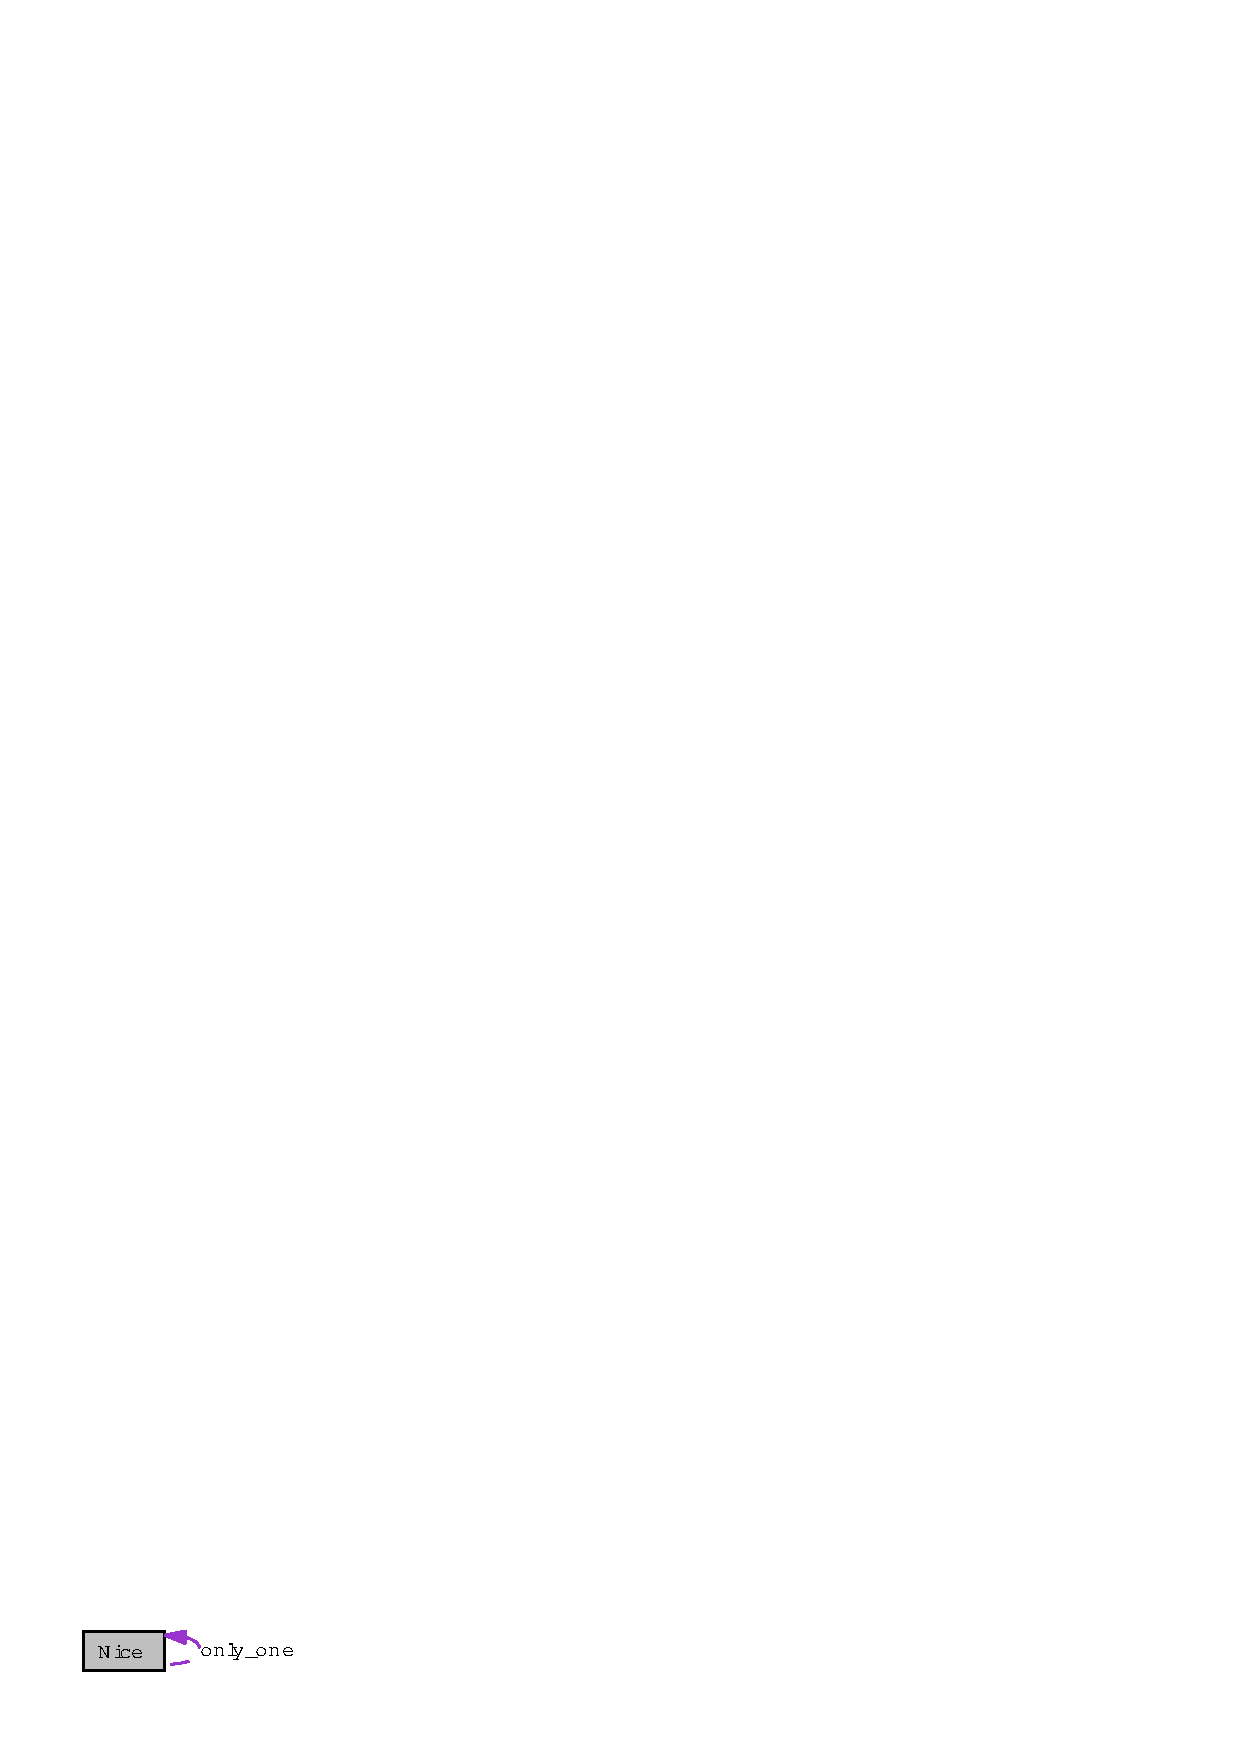
\includegraphics[width=73pt]{classNice__coll__graph}
\end{center}
\end{figure}
\subsection*{Public Member Functions}
\begin{CompactItemize}
\item 
int {\bf get\-Nonnice\-Count} (bool)
\item 
int {\bf get\-Vertex\-Nice\-Val} ({\bf Vertex} const $\ast$const) const 
\item 
bool {\bf find\-Extra\-Point} ({\bf Vertex} const $\ast$const, {\bf vector3} \&, {\bf fp\_\-cit} const \&) const
\item 
bool {\bf update\-Vertex\-Niceness} ({\bf Vertex} $\ast$const)
\item 
bool {\bf set\-Vertex\-Niceness} ({\bf Vertex} $\ast$const, {\bf vec\_\-op} \&)
\item 
bool {\bf get\-Crossed\-Obj\-From\-Vert\-To\-Extra} ({\bf Vertex} const $\ast$const, {\bf vector3} const \&, {\bf vec\_\-op} \&) const
\item 
bool {\bf get\-Crossed\-Obj\-From\-Extra\-To\-Limit} ({\bf vector3} const \&, {\bf vector3} const \&, {\bf vec\_\-op} \&) const
\item 
bool {\bf vertex\-Is\-Nice} ({\bf Vertex} const $\ast$const) const 
\item 
bool {\bf get\-Point\-Outside\-Object} ({\bf Vertex} const $\ast$const, {\bf vector3} \&, {\bf vec\_\-op} \&) const
\item 
void {\bf get\-Crossed\-Objects} ({\bf Vertex} const $\ast$const, {\bf vec\_\-op} \&) const
\item 
void {\bf get\-Vert\-Adj\-Face\-Ray} ({\bf vector3} \&, {\bf vector3} \&, {\bf fp\_\-cit} const \&) const
\item 
void {\bf get\-Penetrated\-Objs} ({\bf vec\_\-fp} \&, {\bf vec\_\-fp} \&, {\bf vec\_\-op} \&) const
\item 
void {\bf get\-Objects\-From\-Edge\-Hits} ({\bf vec\_\-op} \&edge\_\-hits, {\bf vec\_\-op} \&objs) const
\item 
void {\bf find\-Odd\-Objects} ({\bf vec\_\-op} \&, {\bf vec\_\-op} \&) const
\item 
void {\bf get\-Rays\-To\-World\-Limit} ({\bf vector3} const \&, double[6][3]) const 
\item 
void {\bf set\-Vertex\-Nice\-Val} (int const \&, {\bf Vertex} $\ast$const)
\item 
void {\bf find\-Nonnice\-Vertices} (void)
\item 
{\bf face\_\-grp} {\bf find\-Int\-Faces\-Along\-Ray} ({\bf Vertex} const $\ast$const, {\bf vector3} const \&, {\bf vector3} const \&) const
\item 
{\bf vhm\_\-cit} {\bf begin\-Nice} (void) const
\item 
{\bf vhm\_\-cit} {\bf end\-Nice} (void) const
\end{CompactItemize}
\subsection*{Static Public Member Functions}
\begin{CompactItemize}
\item 
static {\bf Nice} \& {\bf instance} (void)
\end{CompactItemize}


\subsection{Member Function Documentation}
\index{Nice@{Nice}!instance@{instance}}
\index{instance@{instance}!Nice@{Nice}}
\subsubsection{\setlength{\rightskip}{0pt plus 5cm}{\bf Nice} \& Nice::instance (void)\hspace{0.3cm}{\tt  [static]}}\label{classNice_0e7a8f2b7f6c9e5a41b4f0a106a7614e}


\index{Nice@{Nice}!getNonniceCount@{getNonniceCount}}
\index{getNonniceCount@{getNonniceCount}!Nice@{Nice}}
\subsubsection{\setlength{\rightskip}{0pt plus 5cm}int Nice::get\-Nonnice\-Count (bool {\em detect\_\-self})}\label{classNice_240dbc4371a3b6931b38dda59bd827a0}


Count the number of nonnice vertices in model. \begin{Desc}
\item[Parameters:]
\begin{description}
\item[\mbox{$\leftarrow$} {\em detect\_\-self}]If true then only count vertices inside their parent object. \end{description}
\end{Desc}
\begin{Desc}
\item[Returns:]Number of nonnice vertices. \end{Desc}
\index{Nice@{Nice}!getVertexNiceVal@{getVertexNiceVal}}
\index{getVertexNiceVal@{getVertexNiceVal}!Nice@{Nice}}
\subsubsection{\setlength{\rightskip}{0pt plus 5cm}int Nice::get\-Vertex\-Nice\-Val ({\bf Vertex} const $\ast$ const {\em v}) const}\label{classNice_b4bb5fcc411699c7a0c937f912ba2cfc}


Get nice value of vertex with code described in \doxyref{nice.cc}{p.}{nice_8cc}. \begin{Desc}
\item[Parameters:]
\begin{description}
\item[\mbox{$\leftarrow$} {\em v}]\doxyref{Vertex}{p.}{classVertex} of interest. \end{description}
\end{Desc}
\begin{Desc}
\item[Returns:]\doxyref{Nice}{p.}{classNice} value of vertex. \end{Desc}
\index{Nice@{Nice}!findExtraPoint@{findExtraPoint}}
\index{findExtraPoint@{findExtraPoint}!Nice@{Nice}}
\subsubsection{\setlength{\rightskip}{0pt plus 5cm}bool Nice::find\-Extra\-Point ({\bf Vertex} const $\ast$ const {\em v}, {\bf vector3} \& {\em extra\_\-obj\_\-pt}, {\bf fp\_\-cit} const \& {\em adjacent\_\-face}) const}\label{classNice_59b64767fd42e4febb07a31037930853}


Identify a location near the vertex of interest guaranteed to be outside of the parent object of vertex. \begin{Desc}
\item[Parameters:]
\begin{description}
\item[\mbox{$\leftarrow$} {\em v}]\doxyref{Vertex}{p.}{classVertex} of interest. \item[\mbox{$\rightarrow$} {\em extra\_\-obj\_\-pt}]Location outside of vertex parent object, if successfully found. \item[\mbox{$\leftarrow$} {\em adjacent\_\-face}]Iterator pointing to vertex adjacent face to use as parent of extracellular location. \end{description}
\end{Desc}
\begin{Desc}
\item[Returns:]1 if extra-object location identified; 0 otherwise. \end{Desc}
\index{Nice@{Nice}!updateVertexNiceness@{updateVertexNiceness}}
\index{updateVertexNiceness@{updateVertexNiceness}!Nice@{Nice}}
\subsubsection{\setlength{\rightskip}{0pt plus 5cm}bool Nice::update\-Vertex\-Niceness ({\bf Vertex} $\ast$ const {\em v})}\label{classNice_cbba0af11271c50201e5d3fdd6c77df5}


Evaluate niceness of vertex with ray tracing and record and return result. \begin{Desc}
\item[Parameters:]
\begin{description}
\item[\mbox{$\leftarrow$} {\em v}]\doxyref{Vertex}{p.}{classVertex} of interest. \end{description}
\end{Desc}
\begin{Desc}
\item[Returns:]True if vertex niceness changed since last check; false otherwise. \end{Desc}
\index{Nice@{Nice}!setVertexNiceness@{setVertexNiceness}}
\index{setVertexNiceness@{setVertexNiceness}!Nice@{Nice}}
\subsubsection{\setlength{\rightskip}{0pt plus 5cm}bool Nice::set\-Vertex\-Niceness ({\bf Vertex} $\ast$ const {\em v}, {\bf vec\_\-op} \& {\em crossed\_\-objects})}\label{classNice_8bda94694b244b3f2c147cdcdc07fc11}


Record new nice value based on collection of objects crossed in ray trace from vertex to world limits. \begin{Desc}
\item[Parameters:]
\begin{description}
\item[\mbox{$\leftarrow$} {\em v}]\doxyref{Vertex}{p.}{classVertex} of interest. \item[\mbox{$\leftarrow$} {\em crossed\_\-objects}]Collection of objects crossed in ray trace from vertex to world limits. \end{description}
\end{Desc}
\begin{Desc}
\item[Returns:]True if vertex niceness changed since last check; false otherwise. \end{Desc}
\index{Nice@{Nice}!getCrossedObjFromVertToExtra@{getCrossedObjFromVertToExtra}}
\index{getCrossedObjFromVertToExtra@{getCrossedObjFromVertToExtra}!Nice@{Nice}}
\subsubsection{\setlength{\rightskip}{0pt plus 5cm}bool Nice::get\-Crossed\-Obj\-From\-Vert\-To\-Extra ({\bf Vertex} const $\ast$ const {\em v}, {\bf vector3} const \& {\em extra\_\-obj\_\-pt}, {\bf vec\_\-op} \& {\em crossed\_\-objects}) const}\label{classNice_c6523ebcf3dd3ab3ae2cc4df228552d1}


Identify and collect objects crossed during ray tracing from input vertex to extra-object location. \begin{Desc}
\item[Parameters:]
\begin{description}
\item[\mbox{$\leftarrow$} {\em v}]\doxyref{Vertex}{p.}{classVertex} of interest. \item[\mbox{$\leftarrow$} {\em extra\_\-obj\_\-pt}]Location guaranteed to be outside vertex parent object. \item[\mbox{$\rightarrow$} {\em crossed\_\-objects}]Collection of object crossed during ray trace from vertex to extra-object point. \end{description}
\end{Desc}
\begin{Desc}
\item[Returns:]True if any edges were intersected by ray; false otherwise. \end{Desc}
\index{Nice@{Nice}!getCrossedObjFromExtraToLimit@{getCrossedObjFromExtraToLimit}}
\index{getCrossedObjFromExtraToLimit@{getCrossedObjFromExtraToLimit}!Nice@{Nice}}
\subsubsection{\setlength{\rightskip}{0pt plus 5cm}bool Nice::get\-Crossed\-Obj\-From\-Extra\-To\-Limit ({\bf vector3} const \& {\em extra\_\-obj\_\-pt}, {\bf vector3} const \& {\em world\_\-limit}, {\bf vec\_\-op} \& {\em crossed\_\-objects}) const}\label{classNice_64131de8b343337f44ac395432301d2f}


Find and return objects crossed during ray trace from extra-object point to world limit. \begin{Desc}
\item[Parameters:]
\begin{description}
\item[\mbox{$\leftarrow$} {\em extra\_\-obj\_\-pt}]Location guaranteed to be outside of object of interest. \item[\mbox{$\leftarrow$} {\em world\_\-limit}]Ray will be traced to the world limit. \item[\mbox{$\rightarrow$} {\em crossed\_\-objects}]Collection of objects crossed during ray trace. \end{description}
\end{Desc}
\begin{Desc}
\item[Returns:]True if any edges were intersected by ray; false otherwise. \end{Desc}
\index{Nice@{Nice}!vertexIsNice@{vertexIsNice}}
\index{vertexIsNice@{vertexIsNice}!Nice@{Nice}}
\subsubsection{\setlength{\rightskip}{0pt plus 5cm}bool Nice::vertex\-Is\-Nice ({\bf Vertex} const $\ast$ const {\em v}) const}\label{classNice_63af897cc818697a97bc5710216be3b7}


Check if vertex is recorded as being nice. \begin{Desc}
\item[Parameters:]
\begin{description}
\item[\mbox{$\leftarrow$} {\em v}]\doxyref{Vertex}{p.}{classVertex} of interest. \end{description}
\end{Desc}
\begin{Desc}
\item[Returns:]True if vertex is nice; false otherwise. \end{Desc}
\index{Nice@{Nice}!getPointOutsideObject@{getPointOutsideObject}}
\index{getPointOutsideObject@{getPointOutsideObject}!Nice@{Nice}}
\subsubsection{\setlength{\rightskip}{0pt plus 5cm}bool Nice::get\-Point\-Outside\-Object ({\bf Vertex} const $\ast$ const {\em v}, {\bf vector3} \& {\em extra\_\-obj\_\-pt}, {\bf vec\_\-op} \& {\em crossed\_\-objects}) const}\label{classNice_69a3315d47dbf2a553d1eb2d84d81b07}


Identify a location guaranteed to be outside the parent object of the vertex of interest and identify object crossings between point and current vertex. \begin{Desc}
\item[Parameters:]
\begin{description}
\item[\mbox{$\leftarrow$} {\em v}]\doxyref{Vertex}{p.}{classVertex} of interest. \item[\mbox{$\rightarrow$} {\em extra\_\-obj\_\-pt}]Location guaranteed to be outside vertex parent object. \item[\mbox{$\rightarrow$} {\em crossed\_\-objects}]Collection of crossed objects between vertex and extra-object location. \end{description}
\end{Desc}
\begin{Desc}
\item[Returns:]True if extra-object location found; false otherwise. \end{Desc}
\index{Nice@{Nice}!getCrossedObjects@{getCrossedObjects}}
\index{getCrossedObjects@{getCrossedObjects}!Nice@{Nice}}
\subsubsection{\setlength{\rightskip}{0pt plus 5cm}void Nice::get\-Crossed\-Objects ({\bf Vertex} const $\ast$ const {\em v}, {\bf vec\_\-op} \& {\em all\_\-crossed\_\-objects}) const}\label{classNice_63e2b67ff6019d9e699ab5fdec131a4e}


Collect and return objects inside which vertex lies as determined by ray tracing. \begin{Desc}
\item[Parameters:]
\begin{description}
\item[\mbox{$\leftarrow$} {\em v}]\doxyref{Vertex}{p.}{classVertex} of interest. \item[\mbox{$\rightarrow$} {\em all\_\-crossed\_\-objects}]Collection of objects inside which vertex lies. \end{description}
\end{Desc}
\index{Nice@{Nice}!getVertAdjFaceRay@{getVertAdjFaceRay}}
\index{getVertAdjFaceRay@{getVertAdjFaceRay}!Nice@{Nice}}
\subsubsection{\setlength{\rightskip}{0pt plus 5cm}void Nice::get\-Vert\-Adj\-Face\-Ray ({\bf vector3} \& {\em centroid}, {\bf vector3} \& {\em extra\_\-obj\_\-pt}, {\bf fp\_\-cit} const \& {\em f}) const}\label{classNice_6ef97573fef2dd9e4028d32404f37dcb}


Calculate ray from adjacent face centroid along face normal small distance. \begin{Desc}
\item[Parameters:]
\begin{description}
\item[\mbox{$\rightarrow$} {\em centroid}]One endpoint of ray. \item[\mbox{$\rightarrow$} {\em extra\_\-obj\_\-pt}]Other endpoint of ray. \item[\mbox{$\leftarrow$} {\em f}]Iterator pointing to adjacent face of vertex of interest. \end{description}
\end{Desc}
\index{Nice@{Nice}!getPenetratedObjs@{getPenetratedObjs}}
\index{getPenetratedObjs@{getPenetratedObjs}!Nice@{Nice}}
\subsubsection{\setlength{\rightskip}{0pt plus 5cm}void Nice::get\-Penetrated\-Objs ({\bf vec\_\-fp} \& {\em crossed\_\-faces}, {\bf vec\_\-fp} \& {\em crossed\_\-faces\_\-on\_\-edge}, {\bf vec\_\-op} \& {\em odd\_\-objects}) const}\label{classNice_530da5dd310d3114b7495593f11047f4}


Collect the objects for which ray not only intersected but certainly changed sides of object, i.e. inside to outside or outside to inside. \begin{Desc}
\item[Parameters:]
\begin{description}
\item[\mbox{$\leftarrow$} {\em crossed\_\-faces}]Faces intersected by ray strictly in face interior. \item[\mbox{$\leftarrow$} {\em crossed\_\-faces\_\-on\_\-edge}]Faces intercted by ray on edge. \item[\mbox{$\rightarrow$} {\em odd\_\-objects}]Objects for which ray changed sides. \end{description}
\end{Desc}
\index{Nice@{Nice}!getObjectsFromEdgeHits@{getObjectsFromEdgeHits}}
\index{getObjectsFromEdgeHits@{getObjectsFromEdgeHits}!Nice@{Nice}}
\subsubsection{\setlength{\rightskip}{0pt plus 5cm}void Nice::get\-Objects\-From\-Edge\-Hits ({\bf vec\_\-op} \& {\em edge\_\-hits}, {\bf vec\_\-op} \& {\em objs}) const}\label{classNice_2d469432f18c28e88b9992aebb132395}


Coalesce pairs of same-object edge hits into single object hits. \begin{Desc}
\item[Parameters:]
\begin{description}
\item[\mbox{$\leftarrow$} {\em edge\_\-hits}]Collection of objects intersected on edge by ray. \item[\mbox{$\rightarrow$} {\em objs}]Collection of intersected objects inferred from edge hits. \end{description}
\end{Desc}
\index{Nice@{Nice}!findOddObjects@{findOddObjects}}
\index{findOddObjects@{findOddObjects}!Nice@{Nice}}
\subsubsection{\setlength{\rightskip}{0pt plus 5cm}void Nice::find\-Odd\-Objects ({\bf vec\_\-op} \&, {\bf vec\_\-op} \&) const}\label{classNice_0ebe9ba0e93a7b97fd324914af605b4d}


\index{Nice@{Nice}!getRaysToWorldLimit@{getRaysToWorldLimit}}
\index{getRaysToWorldLimit@{getRaysToWorldLimit}!Nice@{Nice}}
\subsubsection{\setlength{\rightskip}{0pt plus 5cm}void Nice::get\-Rays\-To\-World\-Limit ({\bf vector3} const \&, double[6][3]) const}\label{classNice_0d7099fe4a836c96f6922e9dd50ffecd}


\index{Nice@{Nice}!setVertexNiceVal@{setVertexNiceVal}}
\index{setVertexNiceVal@{setVertexNiceVal}!Nice@{Nice}}
\subsubsection{\setlength{\rightskip}{0pt plus 5cm}void Nice::set\-Vertex\-Nice\-Val (int const \& {\em newval}, {\bf Vertex} $\ast$ const {\em v})}\label{classNice_7f56f56d6bb507d7d5a13f97a3bdc9c7}


Set nice value of vertex with code described in \doxyref{nice.cc}{p.}{nice_8cc}. \begin{Desc}
\item[Parameters:]
\begin{description}
\item[\mbox{$\leftarrow$} {\em newval}]Set niceval of input vertex to new value. \item[\mbox{$\leftarrow$} {\em v}]\doxyref{Vertex}{p.}{classVertex} of interest. \end{description}
\end{Desc}
\index{Nice@{Nice}!findNonniceVertices@{findNonniceVertices}}
\index{findNonniceVertices@{findNonniceVertices}!Nice@{Nice}}
\subsubsection{\setlength{\rightskip}{0pt plus 5cm}void Nice::find\-Nonnice\-Vertices (void)}\label{classNice_7182baa27280717eaae32dc04543ad00}


Find and record all nonnice vertices in model. \index{Nice@{Nice}!findIntFacesAlongRay@{findIntFacesAlongRay}}
\index{findIntFacesAlongRay@{findIntFacesAlongRay}!Nice@{Nice}}
\subsubsection{\setlength{\rightskip}{0pt plus 5cm}{\bf face\_\-grp} Nice::find\-Int\-Faces\-Along\-Ray ({\bf Vertex} const $\ast$ const {\em v}, {\bf vector3} const \& {\em origin}, {\bf vector3} const \& {\em end}) const}\label{classNice_2588a8f90692a7b20a88a5a8a8c100ce}


Check a collection of faces for interection with input line segment. \begin{Desc}
\item[Parameters:]
\begin{description}
\item[\mbox{$\leftarrow$} {\em v}]\doxyref{Vertex}{p.}{classVertex} of interest. \item[\mbox{$\leftarrow$} {\em origin}]One end of line segment. \item[\mbox{$\leftarrow$} {\em end}]Other end of line segment. \end{description}
\end{Desc}
\begin{Desc}
\item[Returns:]Collection of faces that interect input line segment along an edge or strictly interior of face. \end{Desc}
\index{Nice@{Nice}!beginNice@{beginNice}}
\index{beginNice@{beginNice}!Nice@{Nice}}
\subsubsection{\setlength{\rightskip}{0pt plus 5cm}{\bf vhm\_\-cit} Nice::begin\-Nice (void) const\hspace{0.3cm}{\tt  [inline]}}\label{classNice_bfe44fa4a6225393c93eed8c128af13c}


Get an iterator pointing to first nonnice vertex. \begin{Desc}
\item[Returns:]Iterator pointing to beginning of nonnice vertex container. \end{Desc}
\index{Nice@{Nice}!endNice@{endNice}}
\index{endNice@{endNice}!Nice@{Nice}}
\subsubsection{\setlength{\rightskip}{0pt plus 5cm}{\bf vhm\_\-cit} Nice::end\-Nice (void) const\hspace{0.3cm}{\tt  [inline]}}\label{classNice_400a9465e49d8fcf1339d28eadc2fd1e}


Get an iterator pointing to one past the last nonnice vertex. \begin{Desc}
\item[Returns:]Iterator pointing to one past the last nonnice vertex. \end{Desc}


The documentation for this class was generated from the following files:\begin{CompactItemize}
\item 
{\bf nice.h}\item 
{\bf nice.cc}\end{CompactItemize}

\section{Object Class Reference}
\label{classObject}\index{Object@{Object}}
{\tt \#include $<$object.h$>$}

Collaboration diagram for Object:\begin{figure}[H]
\begin{center}
\leavevmode
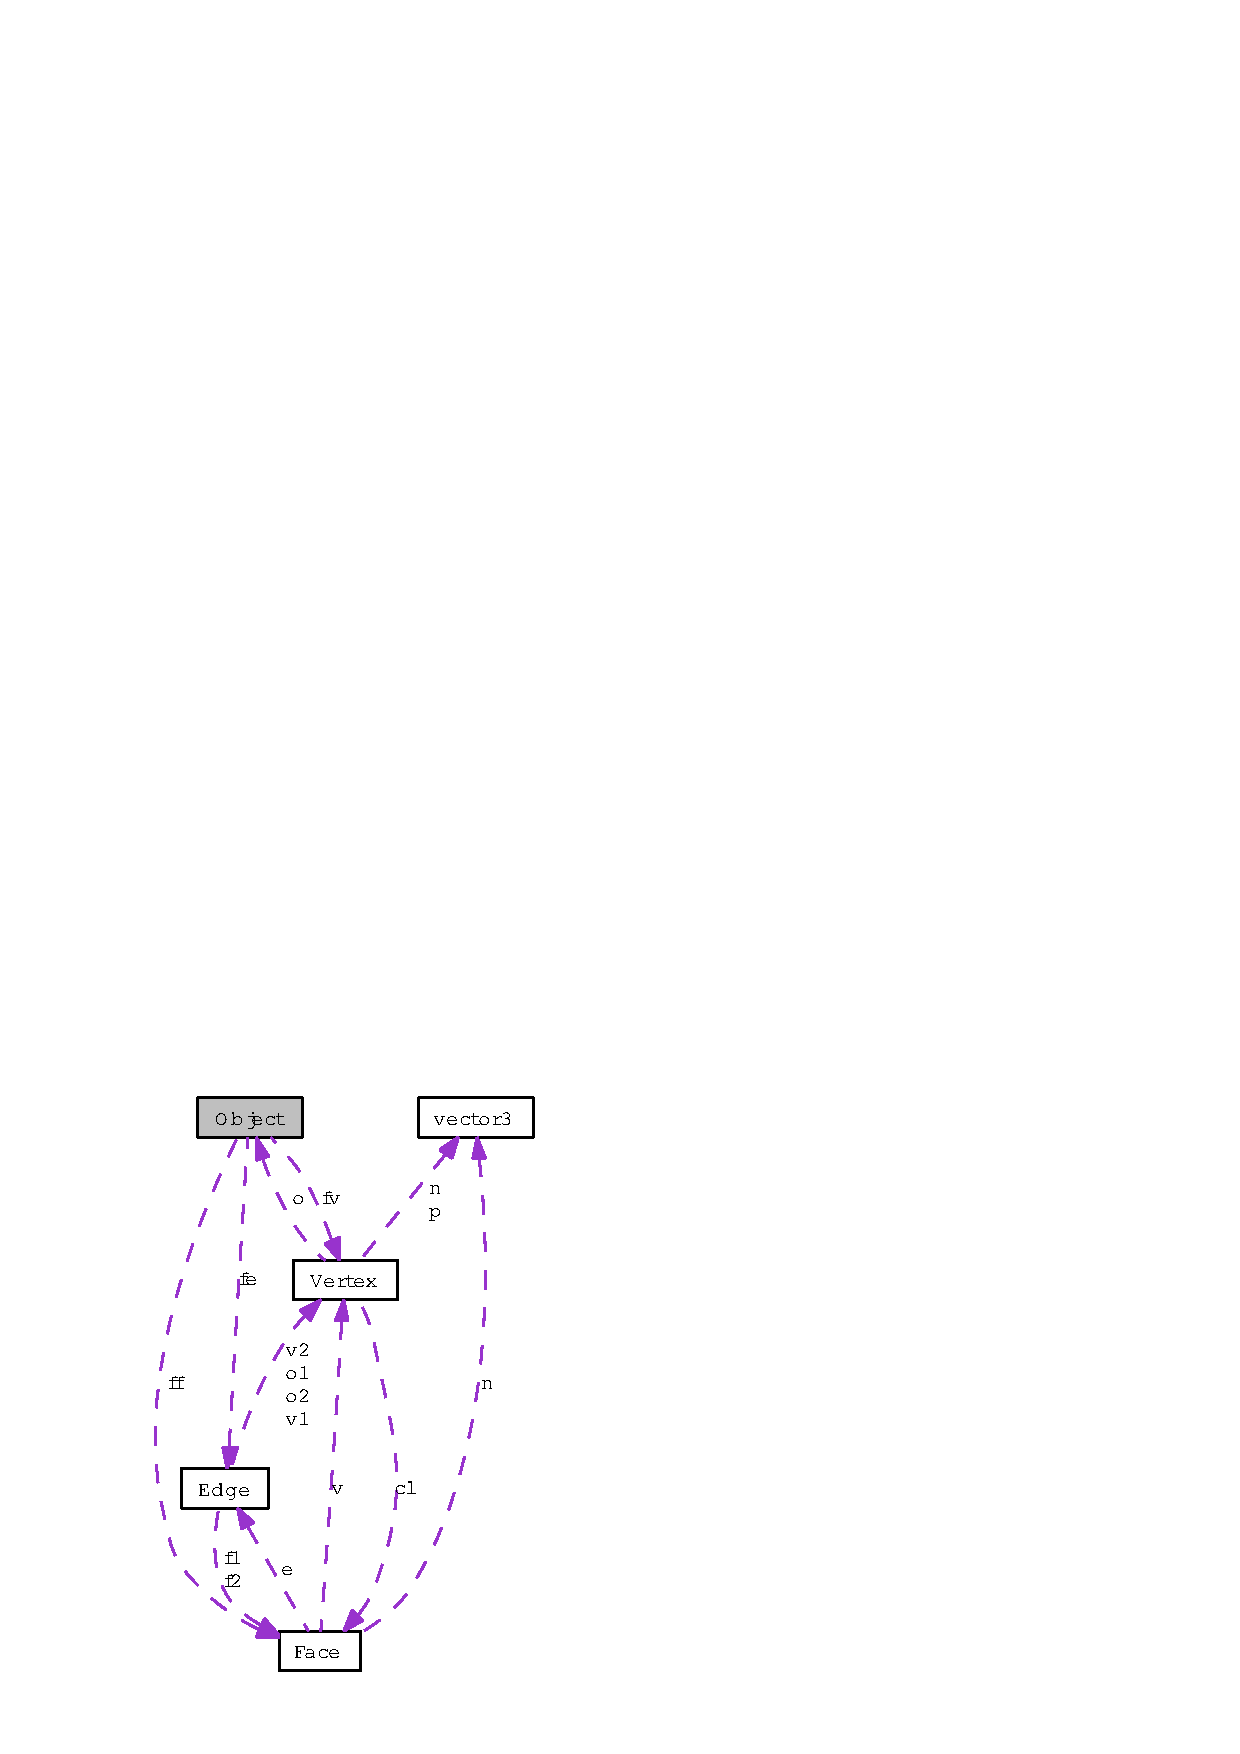
\includegraphics[width=129pt]{classObject__coll__graph}
\end{center}
\end{figure}
\subsection*{Public Member Functions}
\begin{CompactItemize}
\item 
{\bf Object} (std::string)
\item 
{\bf Object} ({\bf Object} const \&)
\item 
{\bf Object} \& {\bf operator=} ({\bf Object} const \&)
\item 
void {\bf find\-Vert\-Adj} (void)
\item 
void {\bf bound\-Object} (double $\ast$const \&) const
\item 
void {\bf set\-FF} ({\bf Face} $\ast$)
\item 
void {\bf set\-FV} ({\bf Vertex} $\ast$)
\item 
{\bf Edge} $\ast$ {\bf get\-FE} (void) const
\item 
{\bf Face} $\ast$ {\bf get\-FF} (void) const
\item 
{\bf Vertex} $\ast$ {\bf get\-FV} (void) const
\item 
std::string const \& {\bf get\-Name} (void) const
\item 
int {\bf set\-Num\-Digits} (void) const
\item 
void {\bf create\-Edges} (void)
\item 
void {\bf process\-Edge} ({\bf Face} $\ast$const, {\bf Vertex} $\ast$const, {\bf Vertex} $\ast$const, {\bf Vertex} $\ast$const, {\bf map\_\-s\_\-ep} \&, int const \&)
\item 
void {\bf create\-Edge} ({\bf Face} $\ast$const, {\bf Vertex} $\ast$const, {\bf Vertex} $\ast$const, {\bf Vertex} $\ast$const, {\bf map\_\-s\_\-ep} \&, int const \&)
\item 
{\bf Edge} $\ast$ {\bf find\-Edge} ({\bf Vertex} const $\ast$const, {\bf Vertex} const $\ast$const, {\bf map\_\-s\_\-ep} const \&, int const \&) const
\item 
std::string {\bf key\-Pair} (int const \&a, int const \&b, int const \&num\_\-digits) const
\end{CompactItemize}
\subsection*{Public Attributes}
\begin{CompactItemize}
\item 
{\bf vec\_\-v} {\bf v}
\item 
{\bf vec\_\-f} {\bf f}
\item 
{\bf vec\_\-e} {\bf e}
\end{CompactItemize}


\subsection{Constructor \& Destructor Documentation}
\index{Object@{Object}!Object@{Object}}
\index{Object@{Object}!Object@{Object}}
\subsubsection{\setlength{\rightskip}{0pt plus 5cm}Object::Object (std::string)}\label{classObject_9726153b1164522a3244fcb885870a99}


\index{Object@{Object}!Object@{Object}}
\index{Object@{Object}!Object@{Object}}
\subsubsection{\setlength{\rightskip}{0pt plus 5cm}Object::Object ({\bf Object} const \&)}\label{classObject_6e166f85639b15a8b8f9b783a6de3b45}




\subsection{Member Function Documentation}
\index{Object@{Object}!operator=@{operator=}}
\index{operator=@{operator=}!Object@{Object}}
\subsubsection{\setlength{\rightskip}{0pt plus 5cm}{\bf Object} \& Object::operator= ({\bf Object} const \&)}\label{classObject_d5a622757f2d91f0b3fc41b8af751d6f}


\index{Object@{Object}!findVertAdj@{findVertAdj}}
\index{findVertAdj@{findVertAdj}!Object@{Object}}
\subsubsection{\setlength{\rightskip}{0pt plus 5cm}void Object::find\-Vert\-Adj (void)}\label{classObject_2489fb94c4141ad5cd692fdb9d9019e9}


Record in vertex class adjacent faces to each vertex in this object. \index{Object@{Object}!boundObject@{boundObject}}
\index{boundObject@{boundObject}!Object@{Object}}
\subsubsection{\setlength{\rightskip}{0pt plus 5cm}void Object::bound\-Object (double $\ast$const \& {\em bounding\_\-box}) const}\label{classObject_40b6fe0262440f577e2c661dc118e9dc}


Compute and return bounding box of this object along principal directions. \begin{Desc}
\item[Parameters:]
\begin{description}
\item[\mbox{$\rightarrow$} {\em bounding\_\-box}]Bounding box of object as (xmin,xmax,ymin,ymax,zmin,zmax). \end{description}
\end{Desc}
\index{Object@{Object}!setFF@{setFF}}
\index{setFF@{setFF}!Object@{Object}}
\subsubsection{\setlength{\rightskip}{0pt plus 5cm}void Object::set\-FF ({\bf Face} $\ast$ {\em fptr})}\label{classObject_b6f62e2bd7a446660a1c4edddbc54c43}


Record pointer to first face in face vector. \begin{Desc}
\item[Parameters:]
\begin{description}
\item[\mbox{$\leftarrow$} {\em fptr}]Pointer to first face. \end{description}
\end{Desc}
\index{Object@{Object}!setFV@{setFV}}
\index{setFV@{setFV}!Object@{Object}}
\subsubsection{\setlength{\rightskip}{0pt plus 5cm}void Object::set\-FV ({\bf Vertex} $\ast$ {\em vv})}\label{classObject_f0c78579e86899e317de5c13ca376578}


Record pointer to first vertex in vertex vector. \begin{Desc}
\item[Parameters:]
\begin{description}
\item[\mbox{$\leftarrow$} {\em vv}]Pointer to first vertex. \end{description}
\end{Desc}
\index{Object@{Object}!getFE@{getFE}}
\index{getFE@{getFE}!Object@{Object}}
\subsubsection{\setlength{\rightskip}{0pt plus 5cm}{\bf Edge} $\ast$ Object::get\-FE (void) const}\label{classObject_f29ab111dc99b3bd5f3aa2909d95cbcb}


Return pointer to recorded first edge in edge vector. \begin{Desc}
\item[Returns:]Pointer to first edge. \end{Desc}
\index{Object@{Object}!getFF@{getFF}}
\index{getFF@{getFF}!Object@{Object}}
\subsubsection{\setlength{\rightskip}{0pt plus 5cm}{\bf Face} $\ast$ Object::get\-FF (void) const}\label{classObject_cf73cd78612c003fcd8898c3a6aadf3a}


Return pointer to recorded first face in face vector. \begin{Desc}
\item[Returns:]Pointer to first face. \end{Desc}
\index{Object@{Object}!getFV@{getFV}}
\index{getFV@{getFV}!Object@{Object}}
\subsubsection{\setlength{\rightskip}{0pt plus 5cm}{\bf Vertex} $\ast$ Object::get\-FV (void) const}\label{classObject_01ba19ef93138092e00449c5a2afe662}


Return pointer to recorded first vertex in vertex vector. \begin{Desc}
\item[Returns:]Pointer to first vertex. \end{Desc}
\index{Object@{Object}!getName@{getName}}
\index{getName@{getName}!Object@{Object}}
\subsubsection{\setlength{\rightskip}{0pt plus 5cm}std::string const \& Object::get\-Name (void) const}\label{classObject_13c8bbe670573a1af1c3c316a57b92a0}


Get recorded name of this object. \begin{Desc}
\item[Returns:]\doxyref{Object}{p.}{classObject} name. \end{Desc}
\index{Object@{Object}!setNumDigits@{setNumDigits}}
\index{setNumDigits@{setNumDigits}!Object@{Object}}
\subsubsection{\setlength{\rightskip}{0pt plus 5cm}int Object::set\-Num\-Digits (void) const}\label{classObject_380cd57bfc576a026727e9b110c13c3c}


Determine the length in digits of largest vertex index. \begin{Desc}
\item[Returns:]Number of digits required for larget vertex index. \end{Desc}
\index{Object@{Object}!createEdges@{createEdges}}
\index{createEdges@{createEdges}!Object@{Object}}
\subsubsection{\setlength{\rightskip}{0pt plus 5cm}void Object::create\-Edges (void)}\label{classObject_f7b4257697cf8cb9bdc289b80596e996}


\index{Object@{Object}!processEdge@{processEdge}}
\index{processEdge@{processEdge}!Object@{Object}}
\subsubsection{\setlength{\rightskip}{0pt plus 5cm}void Object::process\-Edge ({\bf Face} $\ast$ const {\em face}, {\bf Vertex} $\ast$ const {\em va}, {\bf Vertex} $\ast$ const {\em vb}, {\bf Vertex} $\ast$ const {\em vc}, {\bf map\_\-s\_\-ep} \& {\em hm}, int const \& {\em num\_\-digits})}\label{classObject_92a3557cc1df954d7bf78418f79f1a45}


Record input face edge information as \doxyref{Edge}{p.}{classEdge} class instance. \begin{Desc}
\item[Parameters:]
\begin{description}
\item[\mbox{$\leftarrow$} {\em face}]Parent face. \item[\mbox{$\leftarrow$} {\em va}]One vertex of edge from parent face. \item[\mbox{$\leftarrow$} {\em vb}]Other vertex of edge from parent face. \item[\mbox{$\leftarrow$} {\em vc}]\doxyref{Vertex}{p.}{classVertex} from parent face not on edge. \item[\mbox{$\leftarrow$} {\em hm}]Map for finding existing edges with vertex indices as key. \item[\mbox{$\leftarrow$} {\em num\_\-digits}]Number of digits used in maximum integer value. \end{description}
\end{Desc}
\index{Object@{Object}!createEdge@{createEdge}}
\index{createEdge@{createEdge}!Object@{Object}}
\subsubsection{\setlength{\rightskip}{0pt plus 5cm}void Object::create\-Edge ({\bf Face} $\ast$ const {\em face}, {\bf Vertex} $\ast$ const {\em va}, {\bf Vertex} $\ast$ const {\em vb}, {\bf Vertex} $\ast$ const {\em vc}, {\bf map\_\-s\_\-ep} \& {\em hm}, int const \& {\em num\_\-digits})}\label{classObject_4ba1e14d7e3a89f93808bd17b13c63ba}


Create and record new instance of \doxyref{Edge}{p.}{classEdge} class. \begin{Desc}
\item[Parameters:]
\begin{description}
\item[\mbox{$\leftarrow$} {\em face}]Parent face. \item[\mbox{$\leftarrow$} {\em va}]One vertex of edge from parent face. \item[\mbox{$\leftarrow$} {\em vb}]Other vertex of edge from parent face. \item[\mbox{$\leftarrow$} {\em vc}]\doxyref{Vertex}{p.}{classVertex} from parent face not on edge. \item[\mbox{$\leftarrow$} {\em hm}]Map for finding existing edges with vertex indices as key. \item[\mbox{$\leftarrow$} {\em num\_\-digits}]Number of digits used in maximum integer value. \end{description}
\end{Desc}
\index{Object@{Object}!findEdge@{findEdge}}
\index{findEdge@{findEdge}!Object@{Object}}
\subsubsection{\setlength{\rightskip}{0pt plus 5cm}{\bf Edge} $\ast$ Object::find\-Edge ({\bf Vertex} const $\ast$ const {\em va}, {\bf Vertex} const $\ast$ const {\em vb}, {\bf map\_\-s\_\-ep} const \& {\em hm}, int const \& {\em num\_\-digits}) const}\label{classObject_5bf479c6d31a29b8c9cf9a20eb0b923c}


Look for matching recorded edge instance. \begin{Desc}
\item[Parameters:]
\begin{description}
\item[\mbox{$\leftarrow$} {\em va}]One vertex of edge from parent face. \item[\mbox{$\leftarrow$} {\em vb}]Other vertex of edge from parent face. \item[\mbox{$\leftarrow$} {\em hm}]Map for finding existing edges with vertex indices as key. \item[\mbox{$\leftarrow$} {\em num\_\-digits}]Number of digits used in maximum integer value. \end{description}
\end{Desc}
\begin{Desc}
\item[Returns:]\doxyref{Edge}{p.}{classEdge} pointer if match found; NULL otherwise; \end{Desc}
\index{Object@{Object}!keyPair@{keyPair}}
\index{keyPair@{keyPair}!Object@{Object}}
\subsubsection{\setlength{\rightskip}{0pt plus 5cm}std::string Object::key\-Pair (int const \& {\em a}, int const \& {\em b}, int const \& {\em num\_\-digits}) const}\label{classObject_3babf3bd25fd46dfd69898c544c7babd}


Create a unique string from two input integers. \begin{Desc}
\item[Parameters:]
\begin{description}
\item[\mbox{$\leftarrow$} {\em a}]First integer. \item[\mbox{$\leftarrow$} {\em b}]Second integer. \item[\mbox{$\leftarrow$} {\em num\_\-digits}]Number of digits used in maximum integer value. \end{description}
\end{Desc}
\begin{Desc}
\item[Returns:]Unique string including two input integers. \end{Desc}


\subsection{Member Data Documentation}
\index{Object@{Object}!v@{v}}
\index{v@{v}!Object@{Object}}
\subsubsection{\setlength{\rightskip}{0pt plus 5cm}{\bf vec\_\-v} {\bf Object::v}}\label{classObject_f50cb9c150ab8493111dcf29170b23fc}


\index{Object@{Object}!f@{f}}
\index{f@{f}!Object@{Object}}
\subsubsection{\setlength{\rightskip}{0pt plus 5cm}{\bf vec\_\-f} {\bf Object::f}}\label{classObject_ec66102e74e431c089c6ce171e365002}


\index{Object@{Object}!e@{e}}
\index{e@{e}!Object@{Object}}
\subsubsection{\setlength{\rightskip}{0pt plus 5cm}{\bf vec\_\-e} {\bf Object::e}}\label{classObject_8906949fbfe42985f4cd33154abe2835}




The documentation for this class was generated from the following files:\begin{CompactItemize}
\item 
{\bf object.h}\item 
{\bf object.cc}\end{CompactItemize}

\section{hxa7241\_\-graphics::Octree$<$ TYPE $>$ Class Template Reference}
\label{classhxa7241__graphics_1_1Octree}\index{hxa7241_graphics::Octree@{hxa7241\_\-graphics::Octree}}
{\tt \#include $<$Octree.h$>$}

Collaboration diagram for hxa7241\_\-graphics::Octree$<$ TYPE $>$:\begin{figure}[H]
\begin{center}
\leavevmode
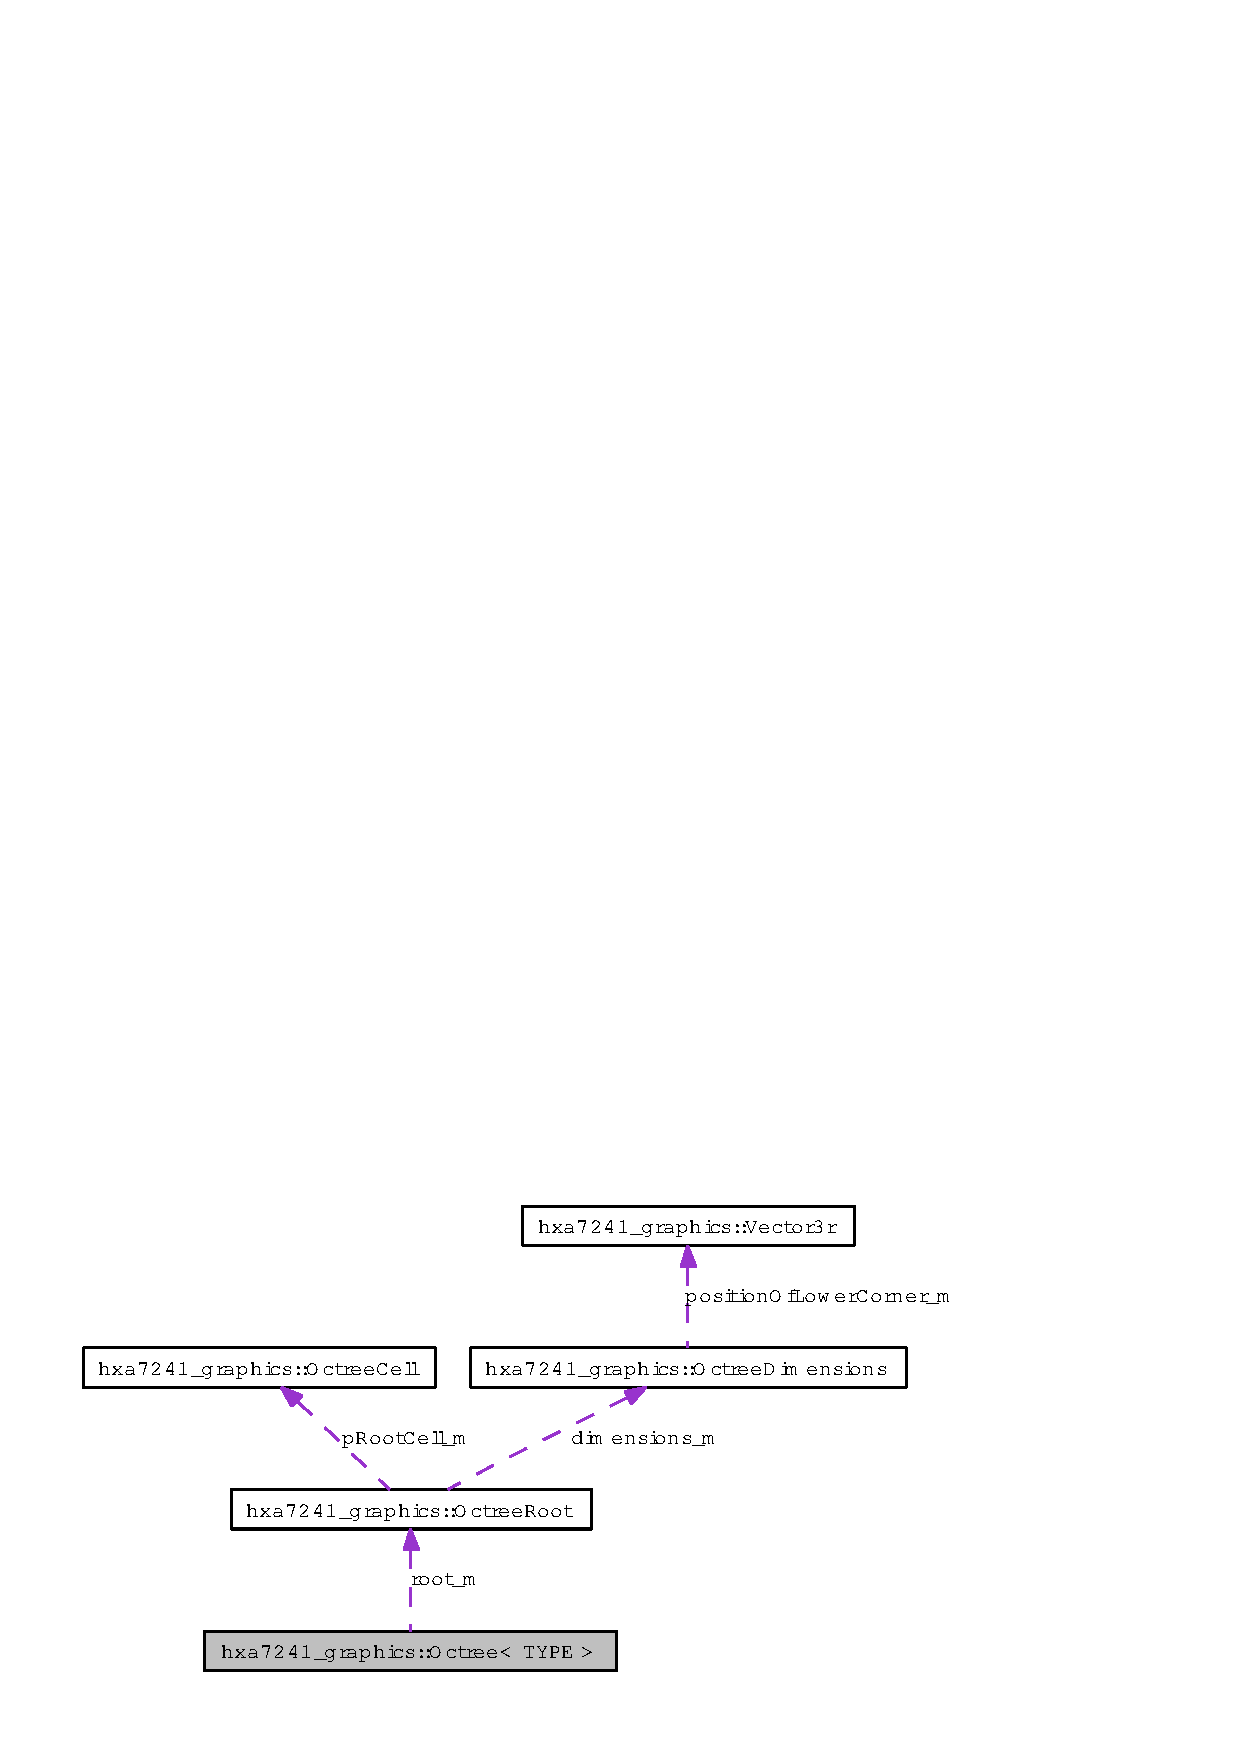
\includegraphics[width=232pt]{classhxa7241__graphics_1_1Octree__coll__graph}
\end{center}
\end{figure}
\subsection*{Public Member Functions}
\begin{CompactItemize}
\item 
{\bf Octree} (const {\bf Vector3r} \&position\-Of\-Lower\-Corner, real size\-Of\-Cube, dword max\-Item\-Count\-Per\-Cell, dword max\-Level\-Count, real min\-Cell\-Size)
\begin{CompactList}\small\item\em standard object services --------------------------------------------------- \item\end{CompactList}\item 
{\bf $\sim$Octree} ()
\item 
{\bf Octree} (const {\bf Octree} \&)
\item 
{\bf Octree} \& {\bf operator=} (const {\bf Octree} \&)
\item 
bool {\bf insert} (const TYPE \&item, const {\bf Octree\-Agent}$<$ TYPE $>$ \&agent)
\begin{CompactList}\small\item\em commands ------------------------------------------------------------------- \item\end{CompactList}\item 
bool {\bf remove} (const TYPE \&item, const {\bf Octree\-Agent}$<$ TYPE $>$ \&agent)
\item 
void {\bf visit} ({\bf Octree\-Visitor}$<$ TYPE $>$ \&visitor) const
\begin{CompactList}\small\item\em queries -------------------------------------------------------------------- \item\end{CompactList}\item 
bool {\bf is\-Empty} () const
\item 
void {\bf get\-Info} (dword \&byte\-Size, dword \&leaf\-Count, dword \&item\-Ref\-Count, dword \&max\-Depth) const
\item 
const {\bf Vector3r} \& {\bf get\-Position} () const
\item 
real {\bf get\-Size} () const
\item 
dword {\bf get\-Max\-Item\-Count\-Per\-Cell} () const
\item 
dword {\bf get\-Max\-Level\-Count} () const
\item 
real {\bf get\-Min\-Cell\-Size} () const
\end{CompactItemize}


\subsection{Detailed Description}
\subsubsection*{template$<$class TYPE$>$ class hxa7241\_\-graphics::Octree$<$ TYPE $>$}

\doxyref{Octree}{p.}{classhxa7241__graphics_1_1Octree} based spatial index.\par
\par


Client must define concrete derivatives of Octree\-Agent$<$Item\-Type$>$ and Octree\-Visitor$<$Item\-Type$>$.\par
\par


max\-Item\-Count\-Per\-Cell is ignored where max\-Level\-Count or min\-Cell\-Size is reached. \par
\par


The octree is cubical and axis aligned, partitions are axis aligned, partitions divide in half, each level partitions the previous level in all three axiss.\par
\par


Storage is contracted or expanded as needed by item insertion and removal. \par
\par


(Occupies, very approximately, 20 bytes per point item. maybe...)\par
\par


\doxyref{Octree}{p.}{classhxa7241__graphics_1_1Octree} is only an index: it points to client items, it does not manage storage of items themselves.\par
\par


\begin{Desc}
\item[See also:]\doxyref{Octree\-Agent}{p.}{classhxa7241__graphics_1_1OctreeAgent} 

\doxyref{Octree\-Visitor}{p.}{classhxa7241__graphics_1_1OctreeVisitor}\end{Desc}
The octree structure follows the Composite pattern.\par
\par


This template wrapper ensures the items indexed by the octree, and the agents and visitors used when accessing them are, of matching types. All algorithmic work is delegated to \doxyref{Octree\-Root}{p.}{classhxa7241__graphics_1_1OctreeRoot} and \doxyref{Octree\-Cell}{p.}{classhxa7241__graphics_1_1OctreeCell} derivatives in Octree\-Implementation, which work with abstract base interfaces and void pointers.\par
\par


For the insertion and removal commands, the agent provides an interface for the octree to query the typeless item, and for the visit query, the visitor provides callbacks to read tree nodes for carrying out the visit operation. 



\subsection{Constructor \& Destructor Documentation}
\index{hxa7241_graphics::Octree@{hxa7241\_\-graphics::Octree}!Octree@{Octree}}
\index{Octree@{Octree}!hxa7241_graphics::Octree@{hxa7241\_\-graphics::Octree}}
\subsubsection{\setlength{\rightskip}{0pt plus 5cm}template$<$class TYPE$>$ {\bf hxa7241\_\-graphics::Octree}$<$ TYPE $>$::{\bf Octree} (const {\bf Vector3r} \& {\em position\-Of\-Lower\-Corner}, real {\em size\-Of\-Cube}, dword {\em max\-Item\-Count\-Per\-Cell}, dword {\em max\-Level\-Count}, real {\em min\-Cell\-Size})\hspace{0.3cm}{\tt  [inline]}}\label{classhxa7241__graphics_1_1Octree_944f0b9fbb05beefb427492604d677ea}


standard object services --------------------------------------------------- 

Constructs a particular format of octree.\par
\par
  $\ast$ size\-Of\-Cube is desired length along a side\par
 $\ast$ max\-Item\-Count\-Per\-Cell is desired max item pointers per leaf\par
 $\ast$ max\-Level\-Count is desired max depth of tree\par
 $\ast$ min\-Cell\-Size is desired min size of cells\par
 \index{hxa7241_graphics::Octree@{hxa7241\_\-graphics::Octree}!~Octree@{$\sim$Octree}}
\index{~Octree@{$\sim$Octree}!hxa7241_graphics::Octree@{hxa7241\_\-graphics::Octree}}
\subsubsection{\setlength{\rightskip}{0pt plus 5cm}template$<$class TYPE$>$ {\bf hxa7241\_\-graphics::Octree}$<$ TYPE $>$::$\sim${\bf Octree} ()\hspace{0.3cm}{\tt  [inline]}}\label{classhxa7241__graphics_1_1Octree_996b0ca6208ac65b4e0fe492ba512de2}


\index{hxa7241_graphics::Octree@{hxa7241\_\-graphics::Octree}!Octree@{Octree}}
\index{Octree@{Octree}!hxa7241_graphics::Octree@{hxa7241\_\-graphics::Octree}}
\subsubsection{\setlength{\rightskip}{0pt plus 5cm}template$<$class TYPE$>$ {\bf hxa7241\_\-graphics::Octree}$<$ TYPE $>$::{\bf Octree} (const {\bf Octree}$<$ TYPE $>$ \&)\hspace{0.3cm}{\tt  [inline]}}\label{classhxa7241__graphics_1_1Octree_bc9d63a9de7ebe339fb59441853d4814}




\subsection{Member Function Documentation}
\index{hxa7241_graphics::Octree@{hxa7241\_\-graphics::Octree}!operator=@{operator=}}
\index{operator=@{operator=}!hxa7241_graphics::Octree@{hxa7241\_\-graphics::Octree}}
\subsubsection{\setlength{\rightskip}{0pt plus 5cm}template$<$class TYPE$>$ {\bf Octree}$<$ TYPE $>$ \& {\bf hxa7241\_\-graphics::Octree}$<$ TYPE $>$::operator= (const {\bf Octree}$<$ TYPE $>$ \&)\hspace{0.3cm}{\tt  [inline]}}\label{classhxa7241__graphics_1_1Octree_55ea755c45f60d1a1546c1e74abadfc4}


Can throw storage allocation exceptions. In such cases the octree is unmodified. \index{hxa7241_graphics::Octree@{hxa7241\_\-graphics::Octree}!insert@{insert}}
\index{insert@{insert}!hxa7241_graphics::Octree@{hxa7241\_\-graphics::Octree}}
\subsubsection{\setlength{\rightskip}{0pt plus 5cm}template$<$class TYPE$>$ bool {\bf hxa7241\_\-graphics::Octree}$<$ TYPE $>$::insert (const TYPE \& {\em item}, const {\bf Octree\-Agent}$<$ TYPE $>$ \& {\em agent})\hspace{0.3cm}{\tt  [inline]}}\label{classhxa7241__graphics_1_1Octree_d46b7fd6b1239727b49462cc05fff5bd}


commands ------------------------------------------------------------------- 

Add pointer(s) to the item to the octree.\par
\par
 (If an item has non-zero volume, it may have pointers in multiple cells.)\par
\par
 \begin{Desc}
\item[Returns:]is the item inserted -- false if item not inside root bound  Can throw storage allocation exceptions. In such cases the octree remains structurally ok, but the item will not be fully added, -- call this method again or the remove method. \end{Desc}
\begin{Desc}
\item[See also:]\doxyref{remove}{p.}{classhxa7241__graphics_1_1Octree_d43ca9852a49ac39915c75886d08e368}, \doxyref{Octree\-Agent}{p.}{classhxa7241__graphics_1_1OctreeAgent} \end{Desc}
\index{hxa7241_graphics::Octree@{hxa7241\_\-graphics::Octree}!remove@{remove}}
\index{remove@{remove}!hxa7241_graphics::Octree@{hxa7241\_\-graphics::Octree}}
\subsubsection{\setlength{\rightskip}{0pt plus 5cm}template$<$class TYPE$>$ bool {\bf hxa7241\_\-graphics::Octree}$<$ TYPE $>$::remove (const TYPE \& {\em item}, const {\bf Octree\-Agent}$<$ TYPE $>$ \& {\em agent})\hspace{0.3cm}{\tt  [inline]}}\label{classhxa7241__graphics_1_1Octree_d43ca9852a49ac39915c75886d08e368}


Removes pointer(s) to the item from the octree.\par
\par
 (If an item has non-zero volume, it may have pointers in multiple cells.)\par
\par
 \begin{Desc}
\item[Returns:]is the item removed -- false if item wasn't present  Can throw storage allocation exceptions. In such cases the octree remains structurally ok, but the item will not be fully removed, -- call this method again or the insert method. \end{Desc}
\begin{Desc}
\item[See also:]\doxyref{insert}{p.}{classhxa7241__graphics_1_1Octree_d46b7fd6b1239727b49462cc05fff5bd}, \doxyref{Octree\-Agent}{p.}{classhxa7241__graphics_1_1OctreeAgent} \end{Desc}
\index{hxa7241_graphics::Octree@{hxa7241\_\-graphics::Octree}!visit@{visit}}
\index{visit@{visit}!hxa7241_graphics::Octree@{hxa7241\_\-graphics::Octree}}
\subsubsection{\setlength{\rightskip}{0pt plus 5cm}template$<$class TYPE$>$ void {\bf hxa7241\_\-graphics::Octree}$<$ TYPE $>$::visit ({\bf Octree\-Visitor}$<$ TYPE $>$ \& {\em visitor}) const\hspace{0.3cm}{\tt  [inline]}}\label{classhxa7241__graphics_1_1Octree_b1e060abcc50911c00dcdd0c295e4402}


queries -------------------------------------------------------------------- 

Execute a visit query operation. \begin{Desc}
\item[See also:]\doxyref{Octree\-Visitor}{p.}{classhxa7241__graphics_1_1OctreeVisitor} \end{Desc}
\index{hxa7241_graphics::Octree@{hxa7241\_\-graphics::Octree}!isEmpty@{isEmpty}}
\index{isEmpty@{isEmpty}!hxa7241_graphics::Octree@{hxa7241\_\-graphics::Octree}}
\subsubsection{\setlength{\rightskip}{0pt plus 5cm}template$<$class TYPE$>$ bool {\bf hxa7241\_\-graphics::Octree}$<$ TYPE $>$::is\-Empty () const\hspace{0.3cm}{\tt  [inline]}}\label{classhxa7241__graphics_1_1Octree_08e61f7746c10d74a3709dd8b7e17583}


Reports if the octree is empty. \index{hxa7241_graphics::Octree@{hxa7241\_\-graphics::Octree}!getInfo@{getInfo}}
\index{getInfo@{getInfo}!hxa7241_graphics::Octree@{hxa7241\_\-graphics::Octree}}
\subsubsection{\setlength{\rightskip}{0pt plus 5cm}template$<$class TYPE$>$ void {\bf hxa7241\_\-graphics::Octree}$<$ TYPE $>$::get\-Info (dword \& {\em byte\-Size}, dword \& {\em leaf\-Count}, dword \& {\em item\-Ref\-Count}, dword \& {\em max\-Depth}) const\hspace{0.3cm}{\tt  [inline]}}\label{classhxa7241__graphics_1_1Octree_dd7f1b0d6725a61023b8115a467a2796}


Provides stats on the octree.\par
\par
  $\ast$ byte\-Size is size in bytes\par
 $\ast$ leaf\-Count is number of leafs\par
 $\ast$ item\-Ref\-Count is total number of item pointers in all leafs\par
 $\ast$ max\-Depth is deepest depth of tree\par
 \index{hxa7241_graphics::Octree@{hxa7241\_\-graphics::Octree}!getPosition@{getPosition}}
\index{getPosition@{getPosition}!hxa7241_graphics::Octree@{hxa7241\_\-graphics::Octree}}
\subsubsection{\setlength{\rightskip}{0pt plus 5cm}template$<$class TYPE$>$ const {\bf Vector3r} \& {\bf hxa7241\_\-graphics::Octree}$<$ TYPE $>$::get\-Position () const\hspace{0.3cm}{\tt  [inline]}}\label{classhxa7241__graphics_1_1Octree_a9e1abf0d8d06acf394a7fcd4d1a7fcb}


Gives the position supplied at construction. \index{hxa7241_graphics::Octree@{hxa7241\_\-graphics::Octree}!getSize@{getSize}}
\index{getSize@{getSize}!hxa7241_graphics::Octree@{hxa7241\_\-graphics::Octree}}
\subsubsection{\setlength{\rightskip}{0pt plus 5cm}template$<$class TYPE$>$ real {\bf hxa7241\_\-graphics::Octree}$<$ TYPE $>$::get\-Size () const\hspace{0.3cm}{\tt  [inline]}}\label{classhxa7241__graphics_1_1Octree_fc7cfe60e40751420cce7ba890b3f010}


Gives the size supplied at construction. \index{hxa7241_graphics::Octree@{hxa7241\_\-graphics::Octree}!getMaxItemCountPerCell@{getMaxItemCountPerCell}}
\index{getMaxItemCountPerCell@{getMaxItemCountPerCell}!hxa7241_graphics::Octree@{hxa7241\_\-graphics::Octree}}
\subsubsection{\setlength{\rightskip}{0pt plus 5cm}template$<$class TYPE$>$ dword {\bf hxa7241\_\-graphics::Octree}$<$ TYPE $>$::get\-Max\-Item\-Count\-Per\-Cell () const\hspace{0.3cm}{\tt  [inline]}}\label{classhxa7241__graphics_1_1Octree_4032abd9e481aa257a3ededb90d3933e}


Gives the leaf pointer limit supplied at construction. \index{hxa7241_graphics::Octree@{hxa7241\_\-graphics::Octree}!getMaxLevelCount@{getMaxLevelCount}}
\index{getMaxLevelCount@{getMaxLevelCount}!hxa7241_graphics::Octree@{hxa7241\_\-graphics::Octree}}
\subsubsection{\setlength{\rightskip}{0pt plus 5cm}template$<$class TYPE$>$ dword {\bf hxa7241\_\-graphics::Octree}$<$ TYPE $>$::get\-Max\-Level\-Count () const\hspace{0.3cm}{\tt  [inline]}}\label{classhxa7241__graphics_1_1Octree_97844414ff11d60b560e20aacb483283}


Gives the depth limit supplied at construction. \index{hxa7241_graphics::Octree@{hxa7241\_\-graphics::Octree}!getMinCellSize@{getMinCellSize}}
\index{getMinCellSize@{getMinCellSize}!hxa7241_graphics::Octree@{hxa7241\_\-graphics::Octree}}
\subsubsection{\setlength{\rightskip}{0pt plus 5cm}template$<$class TYPE$>$ real {\bf hxa7241\_\-graphics::Octree}$<$ TYPE $>$::get\-Min\-Cell\-Size () const\hspace{0.3cm}{\tt  [inline]}}\label{classhxa7241__graphics_1_1Octree_31ddc022702545032fe62edb3ffdf279}


Gives the size limit supplied at construction. 

The documentation for this class was generated from the following file:\begin{CompactItemize}
\item 
{\bf Octree.h}\end{CompactItemize}

\section{Octree\_\-Agent\_\-Face Class Reference}
\label{classOctree__Agent__Face}\index{Octree_Agent_Face@{Octree\_\-Agent\_\-Face}}
{\tt \#include $<$octree\_\-agent\_\-face.h$>$}

Inheritance diagram for Octree\_\-Agent\_\-Face:\begin{figure}[H]
\begin{center}
\leavevmode
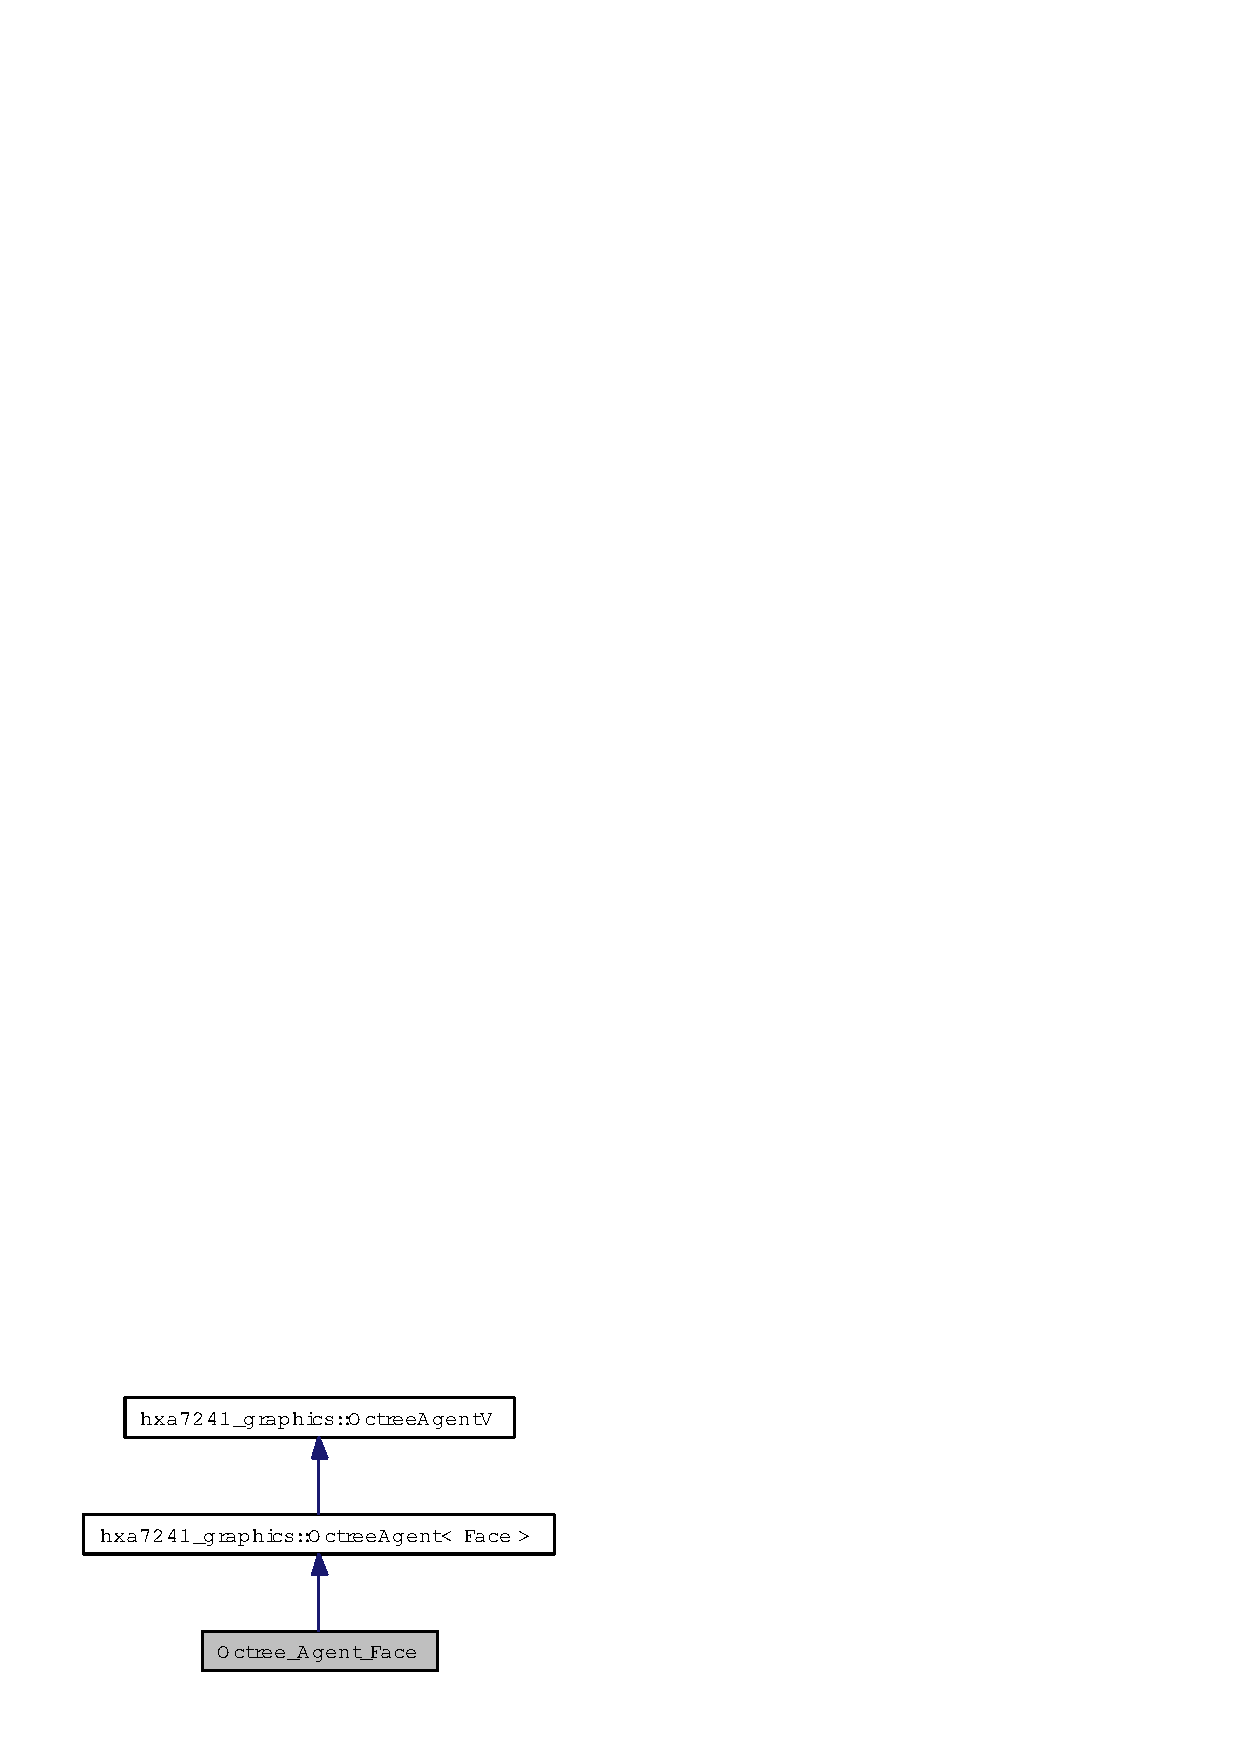
\includegraphics[width=135pt]{classOctree__Agent__Face__inherit__graph}
\end{center}
\end{figure}
Collaboration diagram for Octree\_\-Agent\_\-Face:\begin{figure}[H]
\begin{center}
\leavevmode
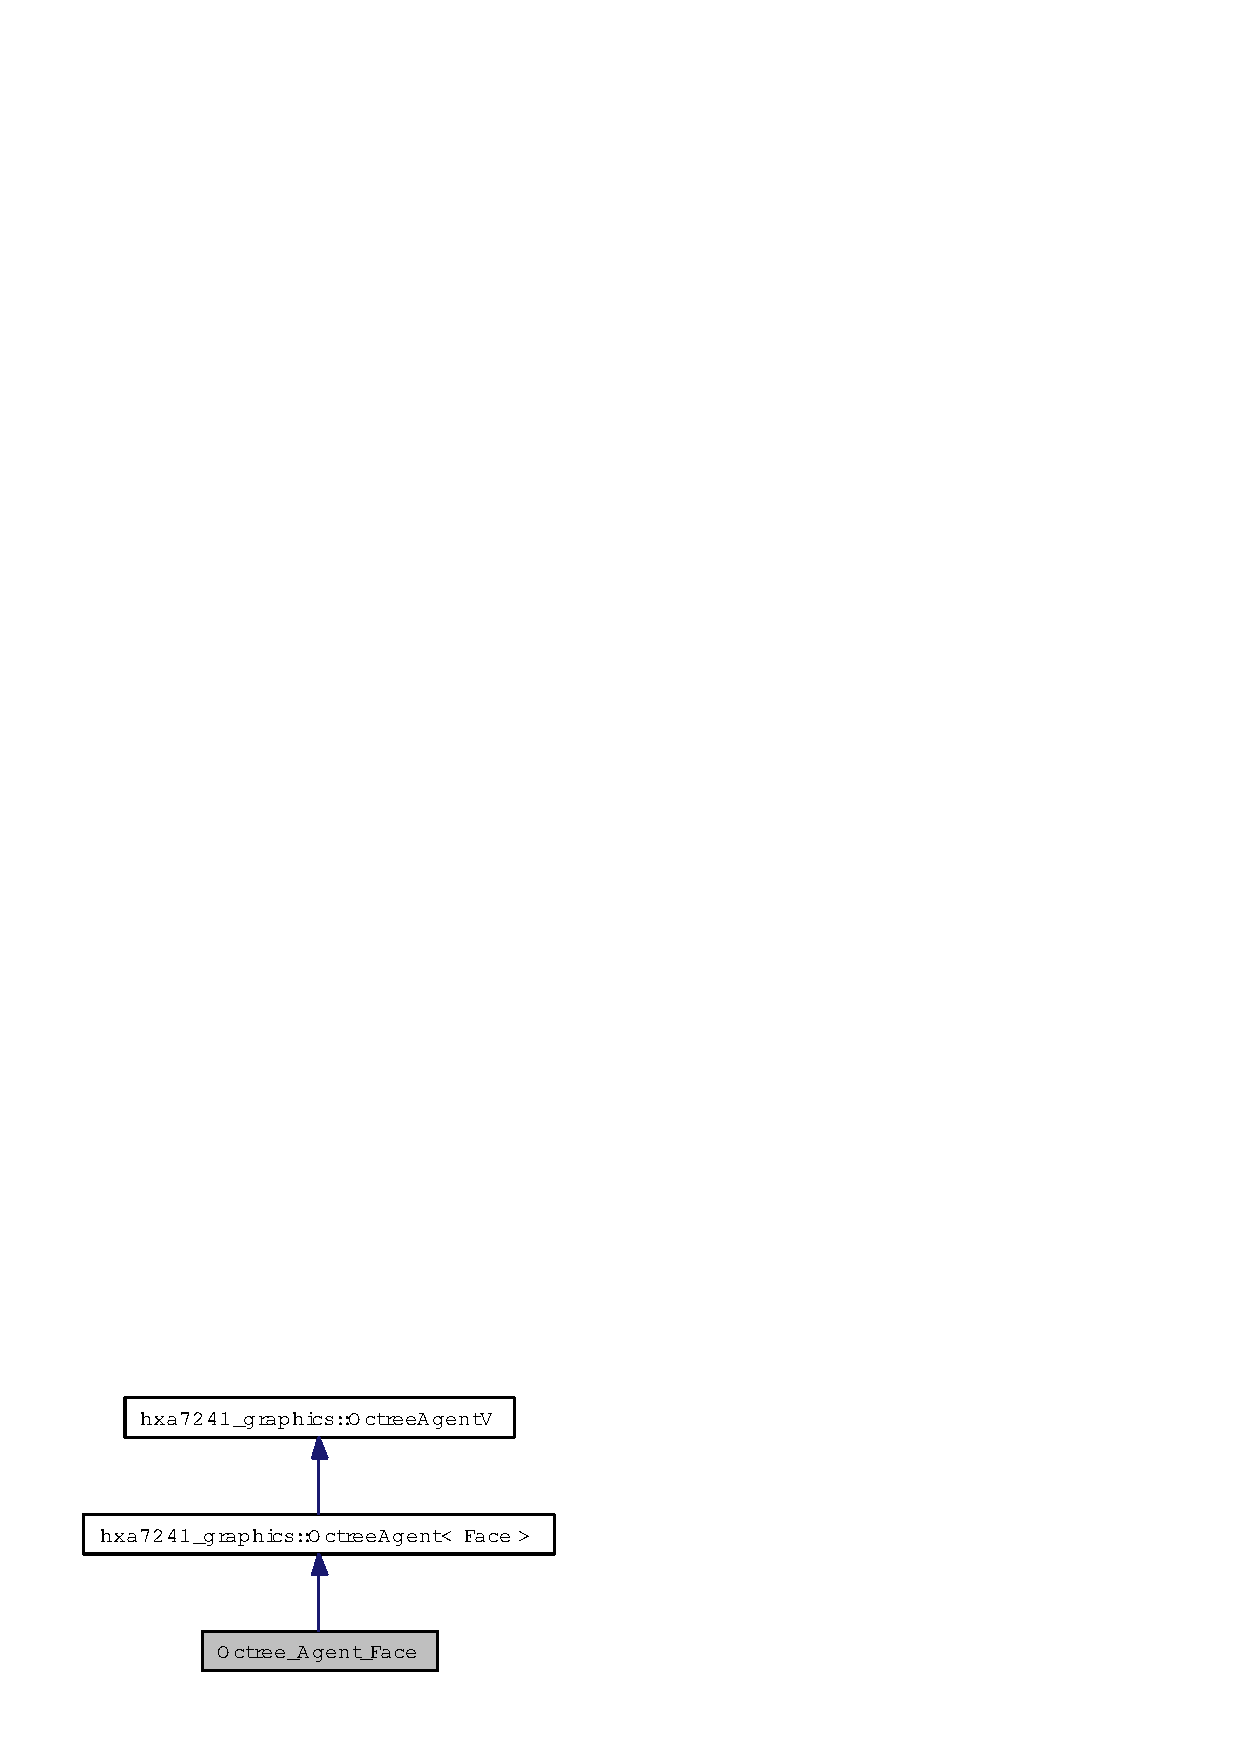
\includegraphics[width=135pt]{classOctree__Agent__Face__coll__graph}
\end{center}
\end{figure}
\subsection*{Public Member Functions}
\begin{CompactItemize}
\item 
{\bf Octree\_\-Agent\_\-Face} ()
\begin{CompactList}\small\item\em standard object services --------------------------------------------------- \item\end{CompactList}\item 
virtual {\bf $\sim$Octree\_\-Agent\_\-Face} ()
\end{CompactItemize}
\subsection*{Protected Member Functions}
\begin{CompactItemize}
\item 
virtual bool {\bf is\-Overlapping\-Cell} (const {\bf Face} \&item, const {\bf Vector3r} \&lower\-Corner, const {\bf Vector3r} \&upper\-Corner) const
\begin{CompactList}\small\item\em queries -------------------------------------------------------------------- \item\end{CompactList}\end{CompactItemize}


\subsection{Constructor \& Destructor Documentation}
\index{Octree_Agent_Face@{Octree\_\-Agent\_\-Face}!Octree_Agent_Face@{Octree\_\-Agent\_\-Face}}
\index{Octree_Agent_Face@{Octree\_\-Agent\_\-Face}!Octree_Agent_Face@{Octree\_\-Agent\_\-Face}}
\subsubsection{\setlength{\rightskip}{0pt plus 5cm}Octree\_\-Agent\_\-Face::Octree\_\-Agent\_\-Face ()\hspace{0.3cm}{\tt  [inline]}}\label{classOctree__Agent__Face_1feec717de681e9d07bb64564f7158b8}


standard object services --------------------------------------------------- 

\index{Octree_Agent_Face@{Octree\_\-Agent\_\-Face}!~Octree_Agent_Face@{$\sim$Octree\_\-Agent\_\-Face}}
\index{~Octree_Agent_Face@{$\sim$Octree\_\-Agent\_\-Face}!Octree_Agent_Face@{Octree\_\-Agent\_\-Face}}
\subsubsection{\setlength{\rightskip}{0pt plus 5cm}virtual Octree\_\-Agent\_\-Face::$\sim$Octree\_\-Agent\_\-Face ()\hspace{0.3cm}{\tt  [inline, virtual]}}\label{classOctree__Agent__Face_a6da65f6f19ccf09d915f089b434bd9a}




\subsection{Member Function Documentation}
\index{Octree_Agent_Face@{Octree\_\-Agent\_\-Face}!isOverlappingCell@{isOverlappingCell}}
\index{isOverlappingCell@{isOverlappingCell}!Octree_Agent_Face@{Octree\_\-Agent\_\-Face}}
\subsubsection{\setlength{\rightskip}{0pt plus 5cm}bool Octree\_\-Agent\_\-Face::is\-Overlapping\-Cell (const {\bf Face} \& {\em item}, const {\bf Vector3r} \& {\em lower\-Corner}, const {\bf Vector3r} \& {\em upper\-Corner}) const\hspace{0.3cm}{\tt  [protected, virtual]}}\label{classOctree__Agent__Face_1fc918ffe7dee3ca4f6a9ccd47f98000}


queries -------------------------------------------------------------------- 

queries -------------------------------------------------------------------- octree agent overrides 

Implements {\bf hxa7241\_\-graphics::Octree\-Agent$<$ Face $>$} \doxyref{}{p.}{classhxa7241__graphics_1_1OctreeAgent_a2df3912d793763643522ffd2f451dbb}.

The documentation for this class was generated from the following files:\begin{CompactItemize}
\item 
{\bf octree\_\-agent\_\-face.h}\item 
{\bf octree\_\-agent\_\-face.cc}\end{CompactItemize}

\section{Octree\_\-Visitor\_\-Check\_\-Face Class Reference}
\label{classOctree__Visitor__Check__Face}\index{Octree_Visitor_Check_Face@{Octree\_\-Visitor\_\-Check\_\-Face}}
{\tt \#include $<$octree\_\-visitor\_\-check\_\-face.h$>$}

Inheritance diagram for Octree\_\-Visitor\_\-Check\_\-Face:\begin{figure}[H]
\begin{center}
\leavevmode
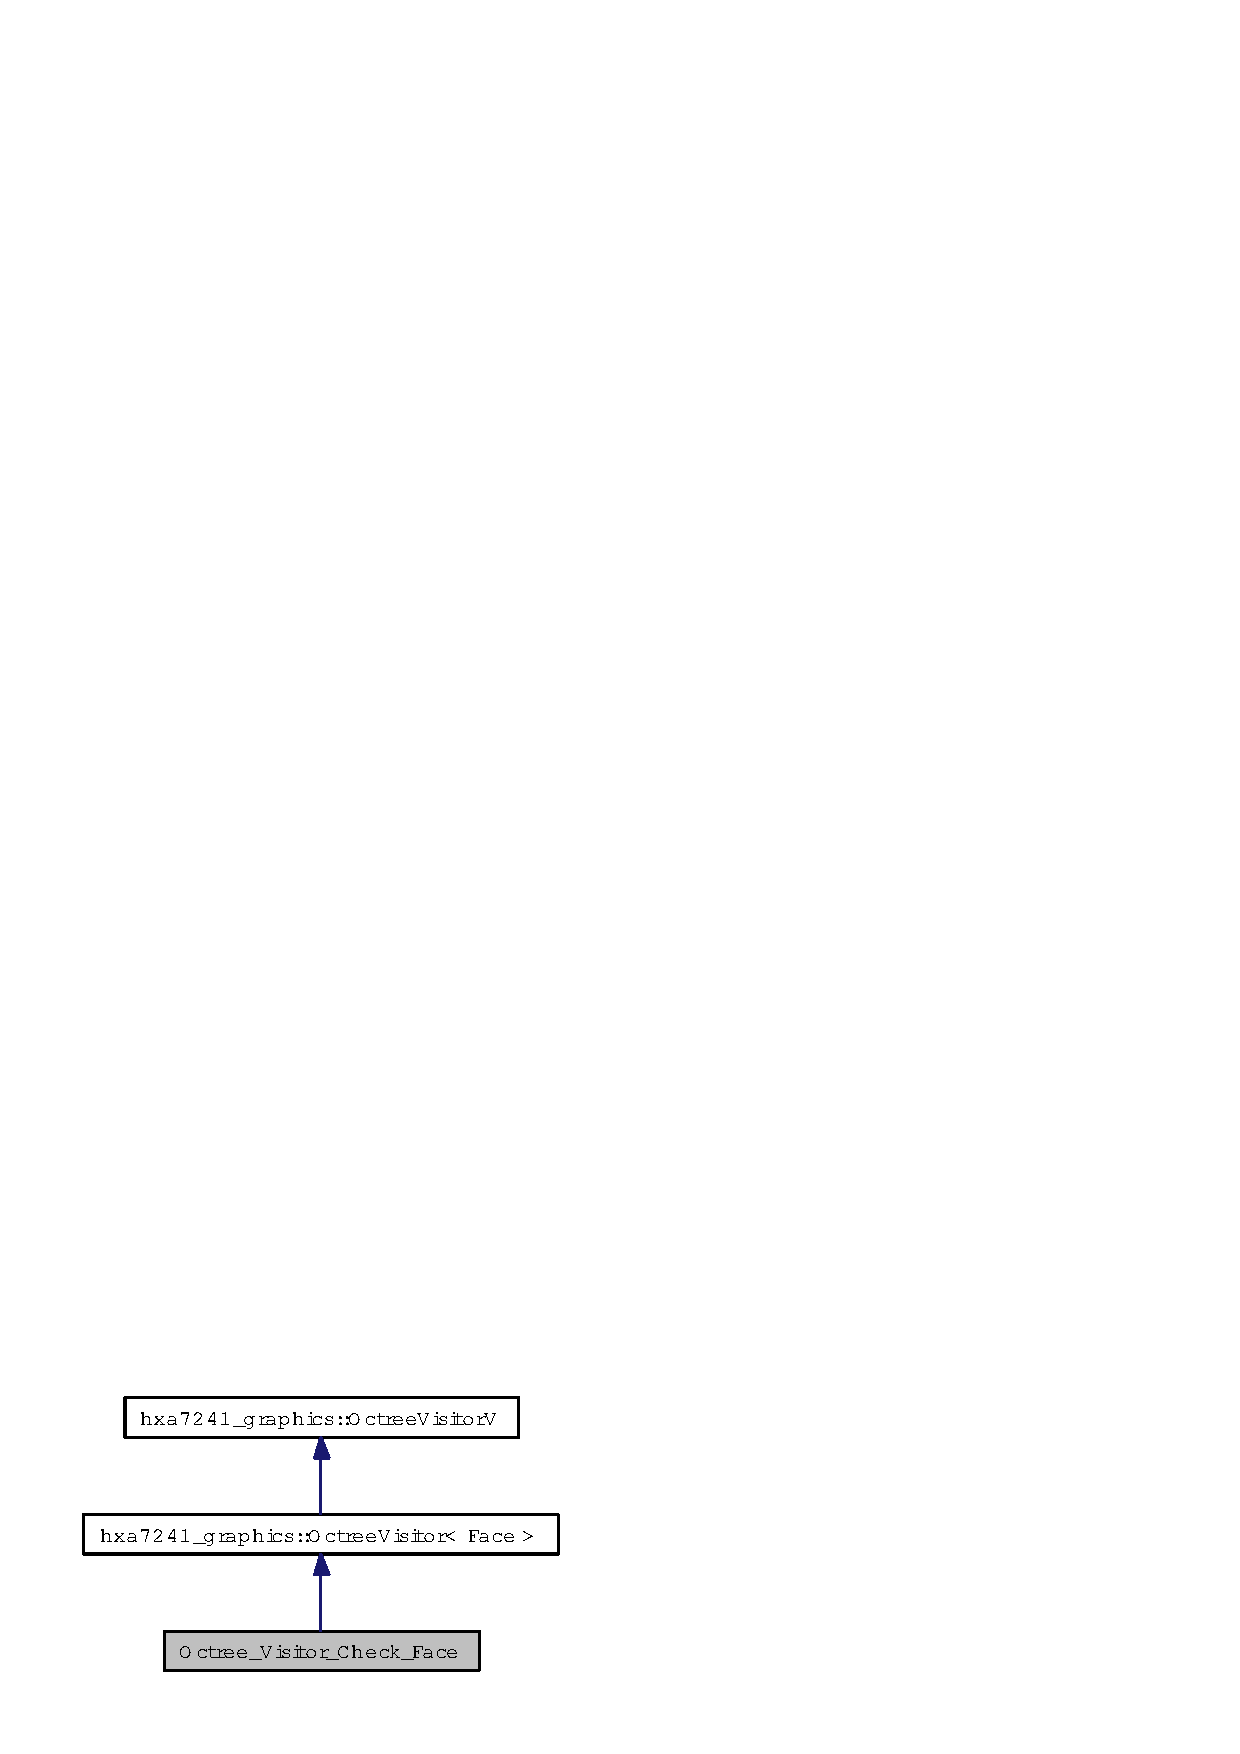
\includegraphics[width=136pt]{classOctree__Visitor__Check__Face__inherit__graph}
\end{center}
\end{figure}
Collaboration diagram for Octree\_\-Visitor\_\-Check\_\-Face:\begin{figure}[H]
\begin{center}
\leavevmode
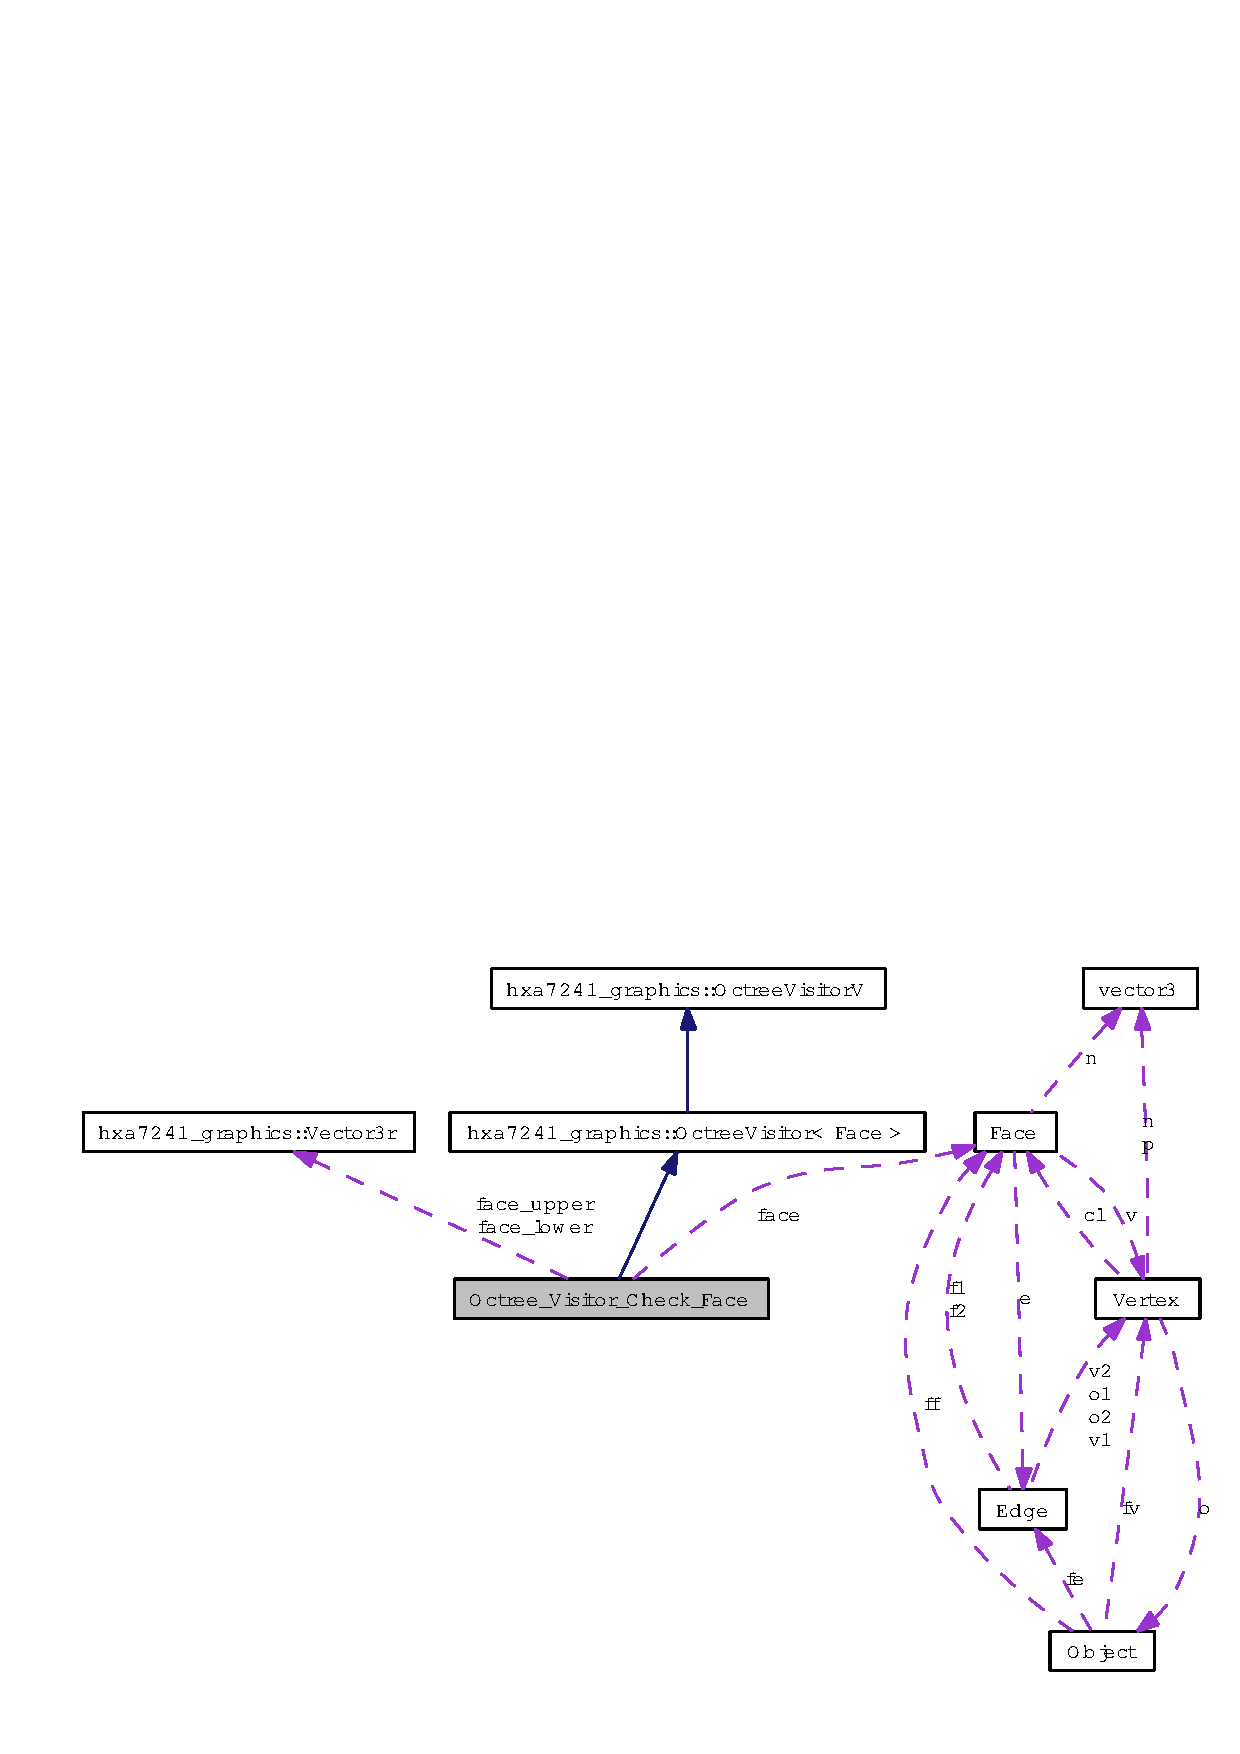
\includegraphics[width=305pt]{classOctree__Visitor__Check__Face__coll__graph}
\end{center}
\end{figure}
\subsection*{Public Member Functions}
\begin{CompactItemize}
\item 
{\bf Octree\_\-Visitor\_\-Check\_\-Face} ({\bf Face} $\ast$f, {\bf Vector3r} low, {\bf Vector3r} up)
\item 
virtual {\bf $\sim$Octree\_\-Visitor\_\-Check\_\-Face} ()
\end{CompactItemize}
\subsection*{Protected Member Functions}
\begin{CompactItemize}
\item 
virtual void {\bf visit\-Root} (const {\bf Octree\-Cell} $\ast$p\-Root\-Cell, const {\bf Octree\-Data} \&octree\-Data)
\begin{CompactList}\small\item\em commands ------------------------------------------------------------------- \item\end{CompactList}\item 
virtual void {\bf visit\-Branch} (const {\bf Octree\-Cell} $\ast$sub\-Cells[8], const {\bf Octree\-Data} \&octree\-Data)
\item 
virtual void {\bf visit\-Leaf} (const Array$<$ const {\bf Face} $\ast$ $>$ \&items, const {\bf Octree\-Data} \&octree\-Data)
\end{CompactItemize}


\subsection{Constructor \& Destructor Documentation}
\index{Octree_Visitor_Check_Face@{Octree\_\-Visitor\_\-Check\_\-Face}!Octree_Visitor_Check_Face@{Octree\_\-Visitor\_\-Check\_\-Face}}
\index{Octree_Visitor_Check_Face@{Octree\_\-Visitor\_\-Check\_\-Face}!Octree_Visitor_Check_Face@{Octree\_\-Visitor\_\-Check\_\-Face}}
\subsubsection{\setlength{\rightskip}{0pt plus 5cm}Octree\_\-Visitor\_\-Check\_\-Face::Octree\_\-Visitor\_\-Check\_\-Face ({\bf Face} $\ast$ {\em f}, {\bf Vector3r} {\em low}, {\bf Vector3r} {\em up})}\label{classOctree__Visitor__Check__Face_6a181d7c974fbe8ac780738f41add22e}


\index{Octree_Visitor_Check_Face@{Octree\_\-Visitor\_\-Check\_\-Face}!~Octree_Visitor_Check_Face@{$\sim$Octree\_\-Visitor\_\-Check\_\-Face}}
\index{~Octree_Visitor_Check_Face@{$\sim$Octree\_\-Visitor\_\-Check\_\-Face}!Octree_Visitor_Check_Face@{Octree\_\-Visitor\_\-Check\_\-Face}}
\subsubsection{\setlength{\rightskip}{0pt plus 5cm}Octree\_\-Visitor\_\-Check\_\-Face::$\sim$Octree\_\-Visitor\_\-Check\_\-Face ()\hspace{0.3cm}{\tt  [virtual]}}\label{classOctree__Visitor__Check__Face_76e69825a8359f0e1cf68cf941acf3e7}




\subsection{Member Function Documentation}
\index{Octree_Visitor_Check_Face@{Octree\_\-Visitor\_\-Check\_\-Face}!visitRoot@{visitRoot}}
\index{visitRoot@{visitRoot}!Octree_Visitor_Check_Face@{Octree\_\-Visitor\_\-Check\_\-Face}}
\subsubsection{\setlength{\rightskip}{0pt plus 5cm}virtual void Octree\_\-Visitor\_\-Check\_\-Face::visit\-Root (const {\bf Octree\-Cell} $\ast$ {\em p\-Root\-Cell}, const {\bf Octree\-Data} \& {\em octree\-Data})\hspace{0.3cm}{\tt  [protected, virtual]}}\label{classOctree__Visitor__Check__Face_b760cdd0db55cd5e0a365007ab400d1a}


commands ------------------------------------------------------------------- 

Called by Octree when visit traversal is at the root.\par
\par
 To continue deeper, implementation calls Octree\-Root::continue\-Visit( p\-Root\-Cell, octree\-Data, $\ast$this ). p\-Root\-Cell can be null.\par
\par
 \begin{Desc}
\item[See also:]Octree\-Data \end{Desc}


Implements {\bf hxa7241\_\-graphics::Octree\-Visitor$<$ TYPE $>$} \doxyref{}{p.}{classhxa7241__graphics_1_1OctreeVisitor_30b2c5b03acb6c75b40d79a86e015878}.\index{Octree_Visitor_Check_Face@{Octree\_\-Visitor\_\-Check\_\-Face}!visitBranch@{visitBranch}}
\index{visitBranch@{visitBranch}!Octree_Visitor_Check_Face@{Octree\_\-Visitor\_\-Check\_\-Face}}
\subsubsection{\setlength{\rightskip}{0pt plus 5cm}virtual void Octree\_\-Visitor\_\-Check\_\-Face::visit\-Branch (const {\bf Octree\-Cell} $\ast$ {\em sub\-Cells}[8], const {\bf Octree\-Data} \& {\em octree\-Data})\hspace{0.3cm}{\tt  [protected, virtual]}}\label{classOctree__Visitor__Check__Face_3846d9a9d6a0c0bf5adf34b324295c87}


Called by Octree when visit traversal is at a branch.\par
\par
 To continue deeper, implementation calls Octree\-Branch::continue\-Visit( sub\-Cells, octree\-Data, sub\-Cell\-Index, $\ast$this ) for any/all sub\-Cell\-Index values. sub\-Cells elements can be null.\par
\par
 \begin{Desc}
\item[See also:]Octree\-Data \end{Desc}


Implements {\bf hxa7241\_\-graphics::Octree\-Visitor$<$ TYPE $>$} \doxyref{}{p.}{classhxa7241__graphics_1_1OctreeVisitor_e62544f5cde1e32e7fd1515e0b8d110d}.\index{Octree_Visitor_Check_Face@{Octree\_\-Visitor\_\-Check\_\-Face}!visitLeaf@{visitLeaf}}
\index{visitLeaf@{visitLeaf}!Octree_Visitor_Check_Face@{Octree\_\-Visitor\_\-Check\_\-Face}}
\subsubsection{\setlength{\rightskip}{0pt plus 5cm}virtual void Octree\_\-Visitor\_\-Check\_\-Face::visit\-Leaf (const Array$<$ const {\bf Face} $\ast$ $>$ \& {\em items}, const {\bf Octree\-Data} \& {\em octree\-Data})\hspace{0.3cm}{\tt  [protected, virtual]}}\label{classOctree__Visitor__Check__Face_dd1c257e364a9c57a803b29899e304f0}




The documentation for this class was generated from the following files:\begin{CompactItemize}
\item 
{\bf octree\_\-visitor\_\-check\_\-face.h}\item 
{\bf octree\_\-visitor\_\-check\_\-face.cc}\end{CompactItemize}

\section{Octree\_\-Visitor\_\-Face Class Reference}
\label{classOctree__Visitor__Face}\index{Octree_Visitor_Face@{Octree\_\-Visitor\_\-Face}}
{\tt \#include $<$octree\_\-visitor\_\-face.h$>$}

Inheritance diagram for Octree\_\-Visitor\_\-Face:\begin{figure}[H]
\begin{center}
\leavevmode
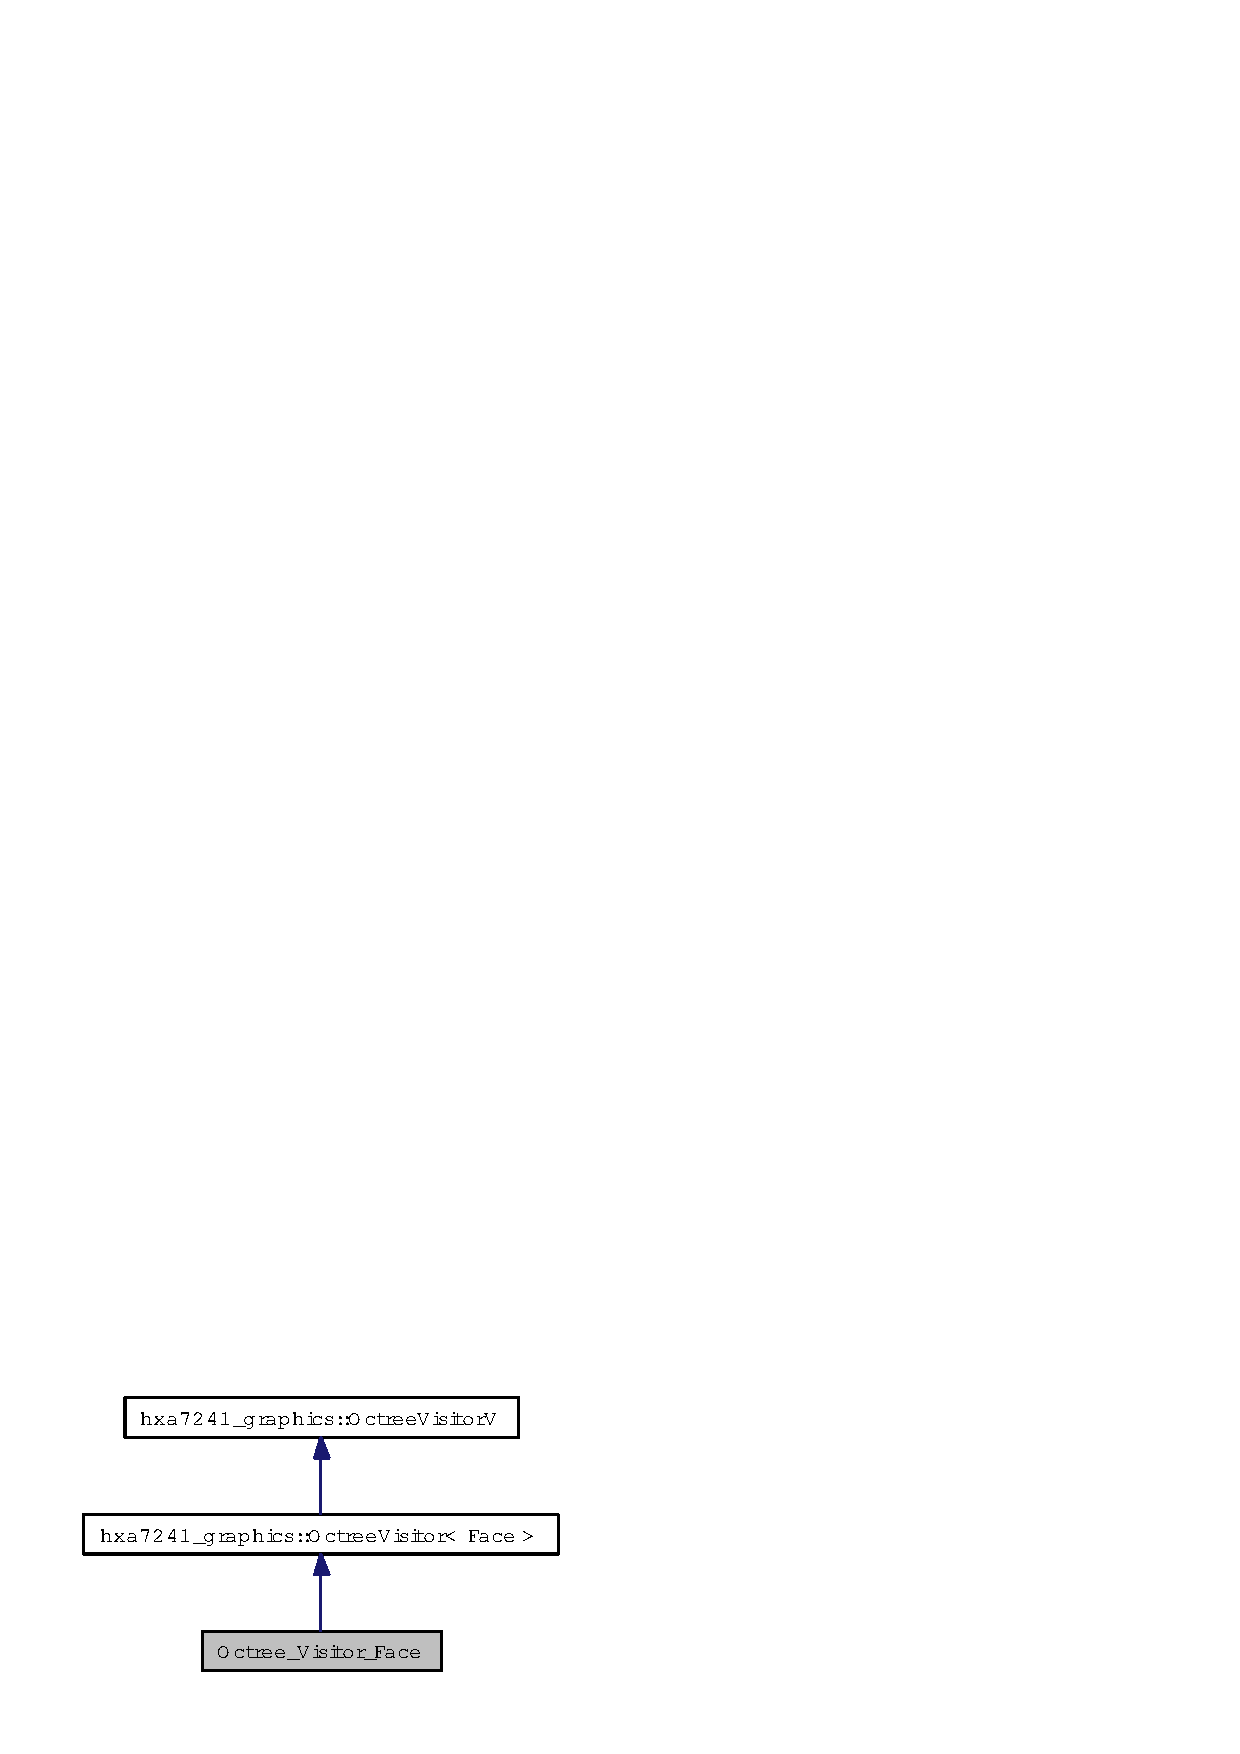
\includegraphics[width=136pt]{classOctree__Visitor__Face__inherit__graph}
\end{center}
\end{figure}
Collaboration diagram for Octree\_\-Visitor\_\-Face:\begin{figure}[H]
\begin{center}
\leavevmode
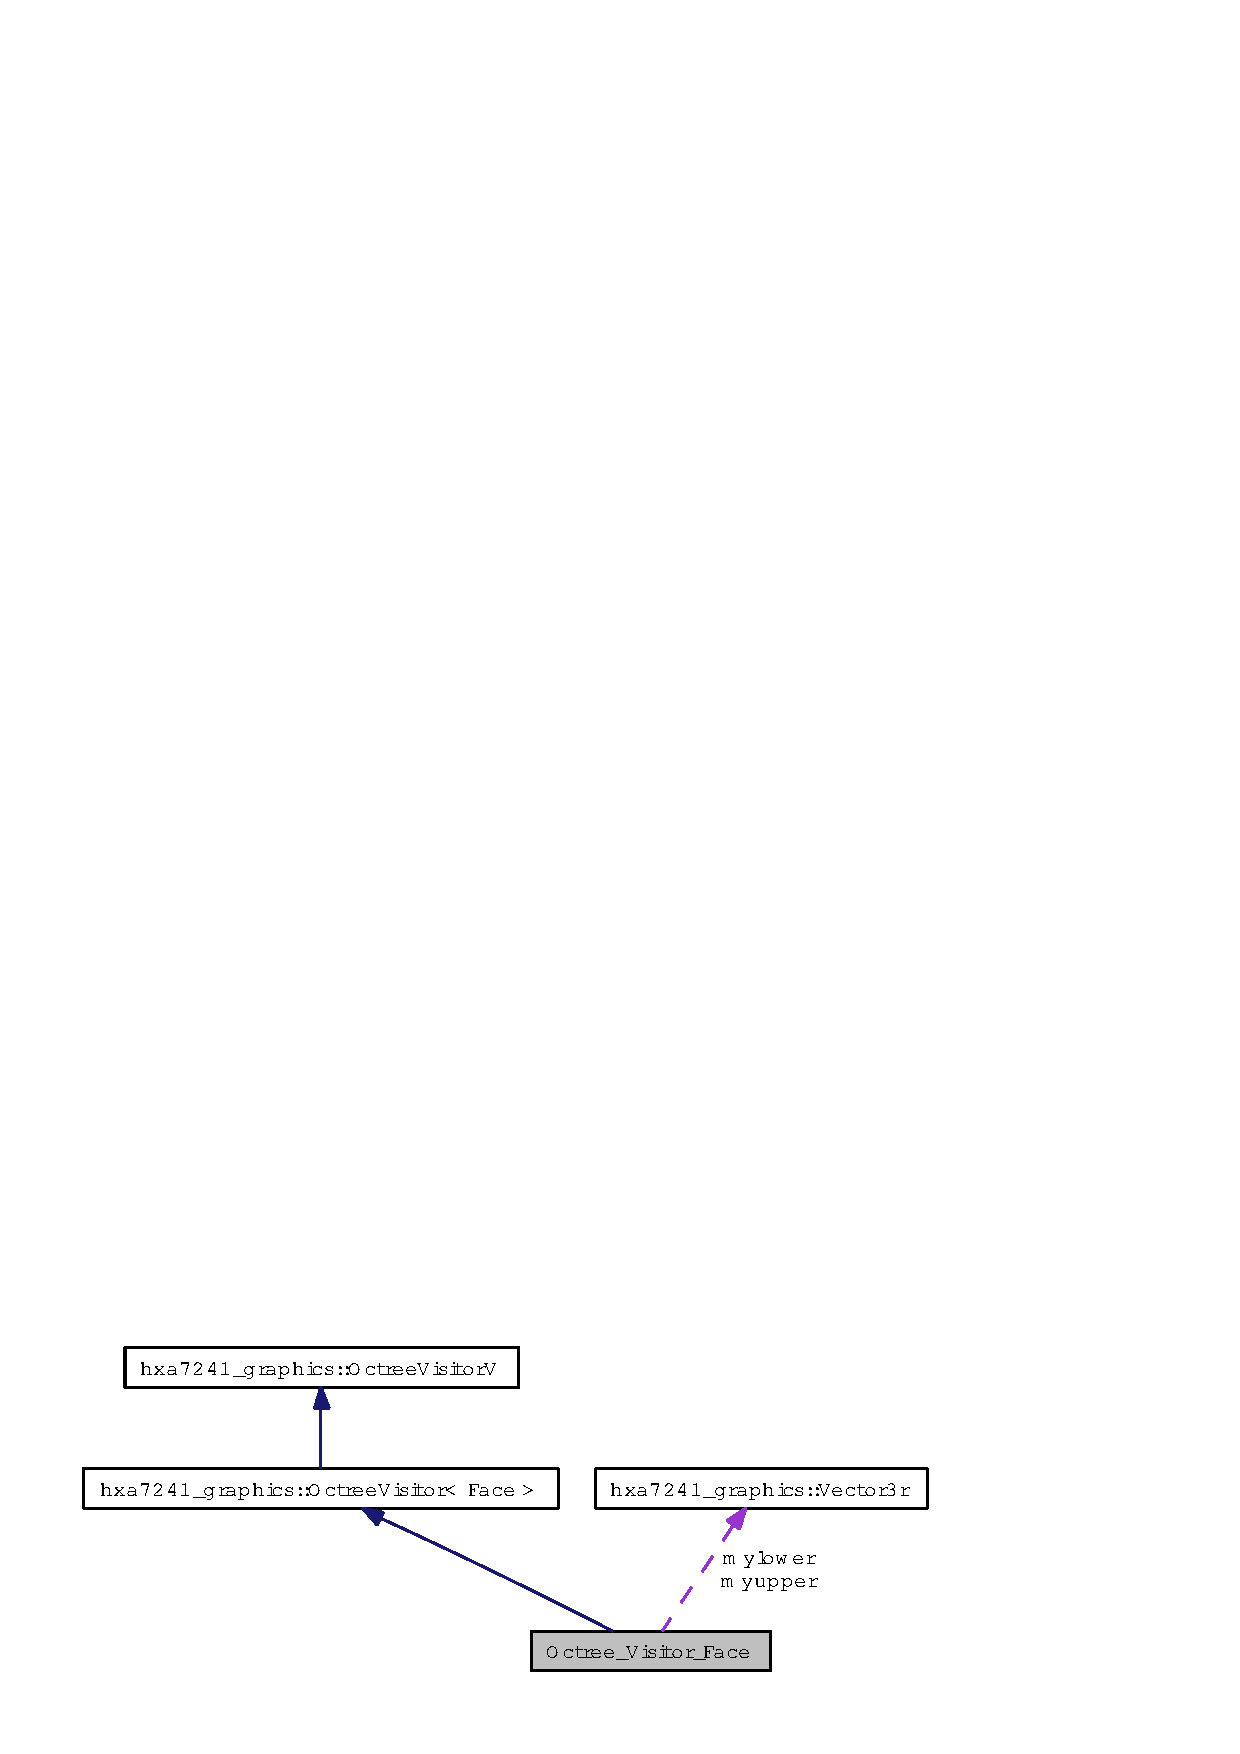
\includegraphics[width=224pt]{classOctree__Visitor__Face__coll__graph}
\end{center}
\end{figure}
\subsection*{Public Member Functions}
\begin{CompactItemize}
\item 
{\bf Octree\_\-Visitor\_\-Face} ({\bf Vector3r}, {\bf Vector3r})
\begin{CompactList}\small\item\em standard object services --------------------------------------------------- \item\end{CompactList}\item 
virtual {\bf $\sim$Octree\_\-Visitor\_\-Face} ()
\item 
{\bf fp\_\-it} {\bf mybegin} (void)
\item 
{\bf fp\_\-it} {\bf myend} (void)
\item 
int {\bf num\_\-faces} (void)
\item 
int {\bf num\_\-leaves} (void)
\end{CompactItemize}
\subsection*{Protected Member Functions}
\begin{CompactItemize}
\item 
virtual void {\bf visit\-Root} (const {\bf Octree\-Cell} $\ast$p\-Root\-Cell, const {\bf Octree\-Data} \&octree\-Data)
\item 
virtual void {\bf visit\-Branch} (const {\bf Octree\-Cell} $\ast$sub\-Cells[8], const {\bf Octree\-Data} \&octree\-Data)
\item 
virtual void {\bf visit\-Leaf} (const Array$<$ const {\bf Face} $\ast$ $>$ \&items, const {\bf Octree\-Data} \&octree\-Data)
\end{CompactItemize}


\subsection{Constructor \& Destructor Documentation}
\index{Octree_Visitor_Face@{Octree\_\-Visitor\_\-Face}!Octree_Visitor_Face@{Octree\_\-Visitor\_\-Face}}
\index{Octree_Visitor_Face@{Octree\_\-Visitor\_\-Face}!Octree_Visitor_Face@{Octree\_\-Visitor\_\-Face}}
\subsubsection{\setlength{\rightskip}{0pt plus 5cm}Octree\_\-Visitor\_\-Face::Octree\_\-Visitor\_\-Face ({\bf Vector3r}, {\bf Vector3r})}\label{classOctree__Visitor__Face_abdc8e42ba87a767d3c10fba6f83ac8c}


standard object services --------------------------------------------------- 

\index{Octree_Visitor_Face@{Octree\_\-Visitor\_\-Face}!~Octree_Visitor_Face@{$\sim$Octree\_\-Visitor\_\-Face}}
\index{~Octree_Visitor_Face@{$\sim$Octree\_\-Visitor\_\-Face}!Octree_Visitor_Face@{Octree\_\-Visitor\_\-Face}}
\subsubsection{\setlength{\rightskip}{0pt plus 5cm}Octree\_\-Visitor\_\-Face::$\sim$Octree\_\-Visitor\_\-Face ()\hspace{0.3cm}{\tt  [virtual]}}\label{classOctree__Visitor__Face_38bbbae9a0088ff39b83894f8085a03f}




\subsection{Member Function Documentation}
\index{Octree_Visitor_Face@{Octree\_\-Visitor\_\-Face}!mybegin@{mybegin}}
\index{mybegin@{mybegin}!Octree_Visitor_Face@{Octree\_\-Visitor\_\-Face}}
\subsubsection{\setlength{\rightskip}{0pt plus 5cm}{\bf fp\_\-it} Octree\_\-Visitor\_\-Face::mybegin (void)\hspace{0.3cm}{\tt  [inline]}}\label{classOctree__Visitor__Face_3bf38552b1e3c6020dd4b6df0f589ae8}


\index{Octree_Visitor_Face@{Octree\_\-Visitor\_\-Face}!myend@{myend}}
\index{myend@{myend}!Octree_Visitor_Face@{Octree\_\-Visitor\_\-Face}}
\subsubsection{\setlength{\rightskip}{0pt plus 5cm}{\bf fp\_\-it} Octree\_\-Visitor\_\-Face::myend (void)\hspace{0.3cm}{\tt  [inline]}}\label{classOctree__Visitor__Face_ca7ed3d14c0016a7c7d4be0588b699fc}


\index{Octree_Visitor_Face@{Octree\_\-Visitor\_\-Face}!num_faces@{num\_\-faces}}
\index{num_faces@{num\_\-faces}!Octree_Visitor_Face@{Octree\_\-Visitor\_\-Face}}
\subsubsection{\setlength{\rightskip}{0pt plus 5cm}int Octree\_\-Visitor\_\-Face::num\_\-faces (void)\hspace{0.3cm}{\tt  [inline]}}\label{classOctree__Visitor__Face_9901ce5624d28305a1b4ca068887b06f}


\index{Octree_Visitor_Face@{Octree\_\-Visitor\_\-Face}!num_leaves@{num\_\-leaves}}
\index{num_leaves@{num\_\-leaves}!Octree_Visitor_Face@{Octree\_\-Visitor\_\-Face}}
\subsubsection{\setlength{\rightskip}{0pt plus 5cm}int Octree\_\-Visitor\_\-Face::num\_\-leaves (void)\hspace{0.3cm}{\tt  [inline]}}\label{classOctree__Visitor__Face_48cd59c487907434b9e2c09a3fa4ef52}


\index{Octree_Visitor_Face@{Octree\_\-Visitor\_\-Face}!visitRoot@{visitRoot}}
\index{visitRoot@{visitRoot}!Octree_Visitor_Face@{Octree\_\-Visitor\_\-Face}}
\subsubsection{\setlength{\rightskip}{0pt plus 5cm}virtual void Octree\_\-Visitor\_\-Face::visit\-Root (const {\bf Octree\-Cell} $\ast$ {\em p\-Root\-Cell}, const {\bf Octree\-Data} \& {\em octree\-Data})\hspace{0.3cm}{\tt  [protected, virtual]}}\label{classOctree__Visitor__Face_0012a0413872dccf1c1358be7b4b9bc0}


commands ------------------------------------------------------------------- octree visitor overrides 

Implements {\bf hxa7241\_\-graphics::Octree\-Visitor$<$ TYPE $>$} \doxyref{}{p.}{classhxa7241__graphics_1_1OctreeVisitor_30b2c5b03acb6c75b40d79a86e015878}.\index{Octree_Visitor_Face@{Octree\_\-Visitor\_\-Face}!visitBranch@{visitBranch}}
\index{visitBranch@{visitBranch}!Octree_Visitor_Face@{Octree\_\-Visitor\_\-Face}}
\subsubsection{\setlength{\rightskip}{0pt plus 5cm}virtual void Octree\_\-Visitor\_\-Face::visit\-Branch (const {\bf Octree\-Cell} $\ast$ {\em sub\-Cells}[8], const {\bf Octree\-Data} \& {\em octree\-Data})\hspace{0.3cm}{\tt  [protected, virtual]}}\label{classOctree__Visitor__Face_982568defaf668997aceedd9eb69ff15}


Called by Octree when visit traversal is at a branch.\par
\par
 To continue deeper, implementation calls Octree\-Branch::continue\-Visit( sub\-Cells, octree\-Data, sub\-Cell\-Index, $\ast$this ) for any/all sub\-Cell\-Index values. sub\-Cells elements can be null.\par
\par
 \begin{Desc}
\item[See also:]Octree\-Data \end{Desc}


Implements {\bf hxa7241\_\-graphics::Octree\-Visitor$<$ TYPE $>$} \doxyref{}{p.}{classhxa7241__graphics_1_1OctreeVisitor_e62544f5cde1e32e7fd1515e0b8d110d}.\index{Octree_Visitor_Face@{Octree\_\-Visitor\_\-Face}!visitLeaf@{visitLeaf}}
\index{visitLeaf@{visitLeaf}!Octree_Visitor_Face@{Octree\_\-Visitor\_\-Face}}
\subsubsection{\setlength{\rightskip}{0pt plus 5cm}virtual void Octree\_\-Visitor\_\-Face::visit\-Leaf (const Array$<$ const {\bf Face} $\ast$ $>$ \& {\em items}, const {\bf Octree\-Data} \& {\em octree\-Data})\hspace{0.3cm}{\tt  [protected, virtual]}}\label{classOctree__Visitor__Face_92c63f2034aab5e10c47bcfb8fe1ee61}




The documentation for this class was generated from the following files:\begin{CompactItemize}
\item 
{\bf octree\_\-visitor\_\-face.h}\item 
{\bf octree\_\-visitor\_\-face.cc}\end{CompactItemize}

\section{Octree\_\-Visitor\_\-Measure Class Reference}
\label{classOctree__Visitor__Measure}\index{Octree_Visitor_Measure@{Octree\_\-Visitor\_\-Measure}}
{\tt \#include $<$octree\_\-visitor\_\-measure.h$>$}

Inheritance diagram for Octree\_\-Visitor\_\-Measure:\begin{figure}[H]
\begin{center}
\leavevmode
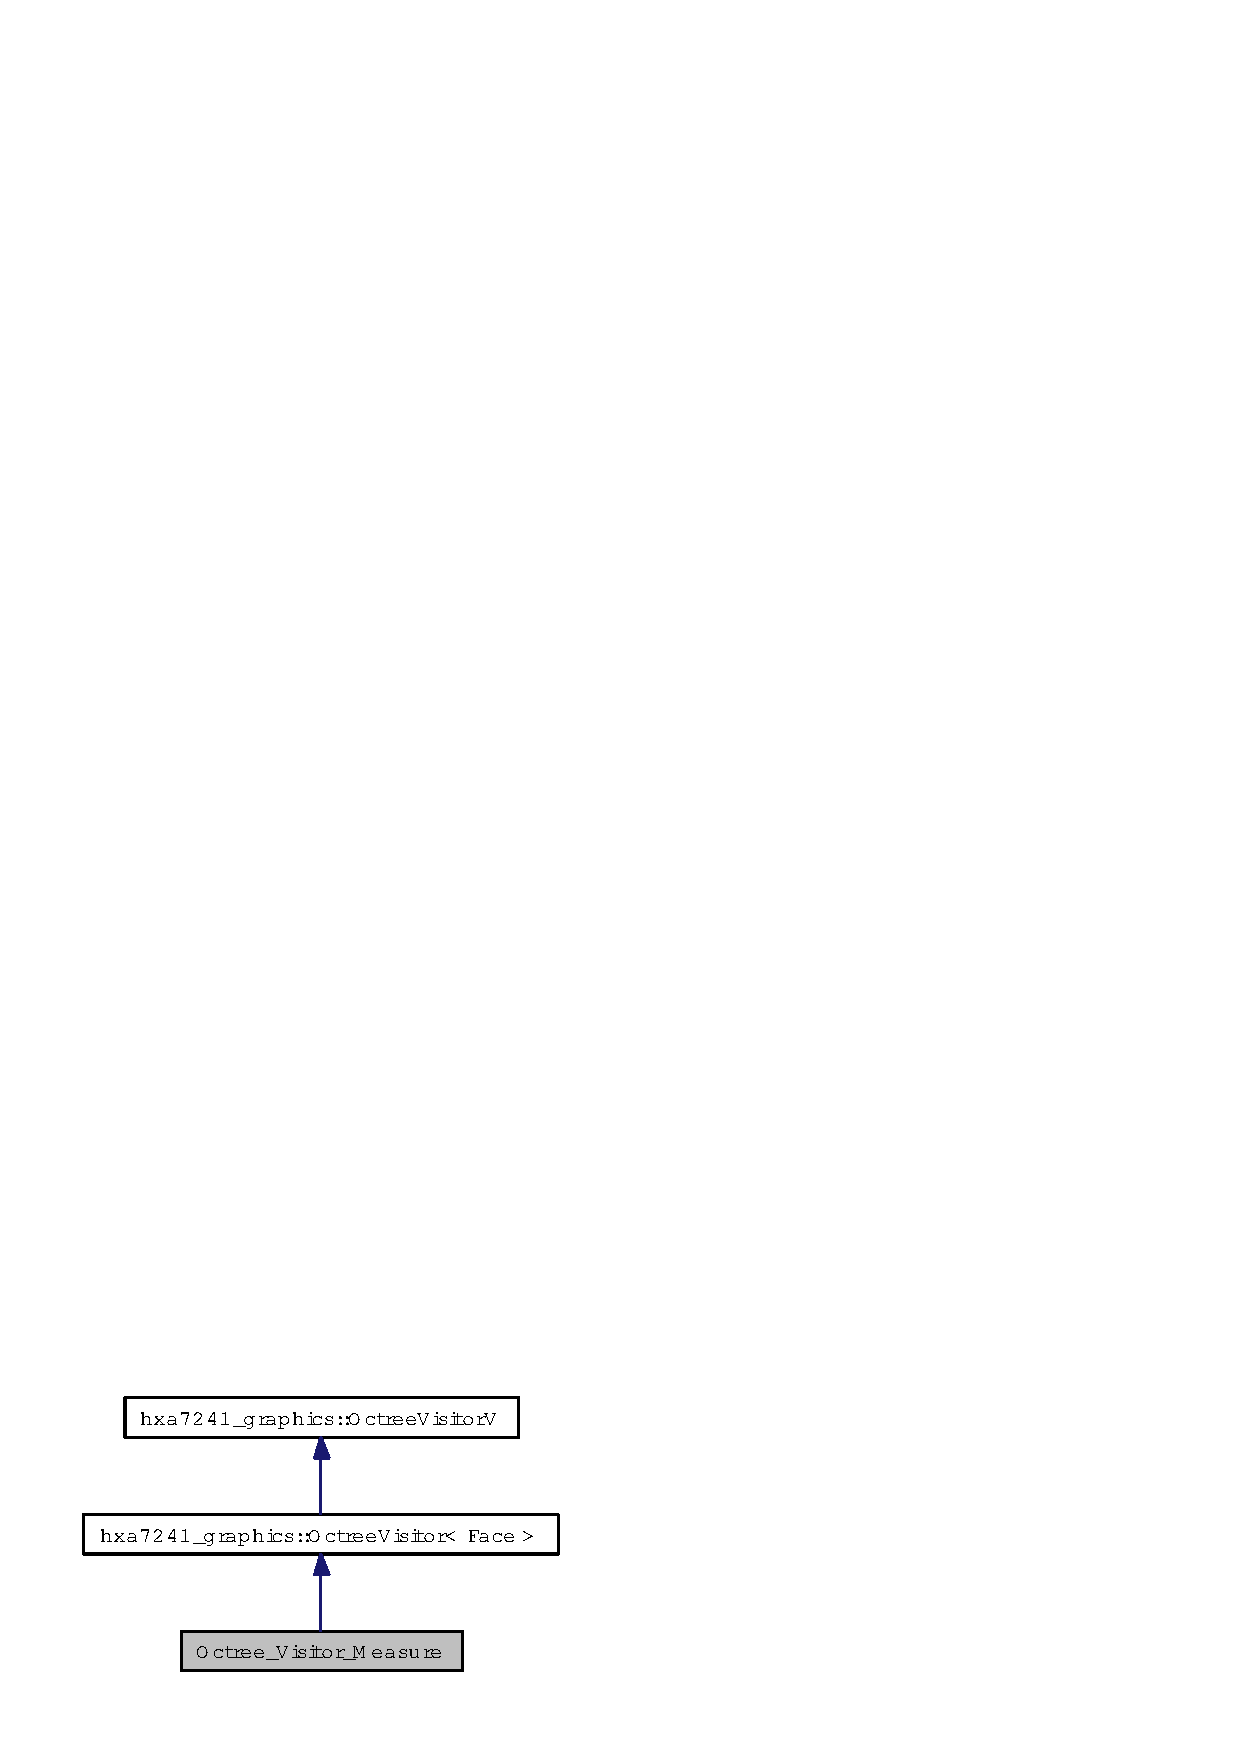
\includegraphics[width=136pt]{classOctree__Visitor__Measure__inherit__graph}
\end{center}
\end{figure}
Collaboration diagram for Octree\_\-Visitor\_\-Measure:\begin{figure}[H]
\begin{center}
\leavevmode
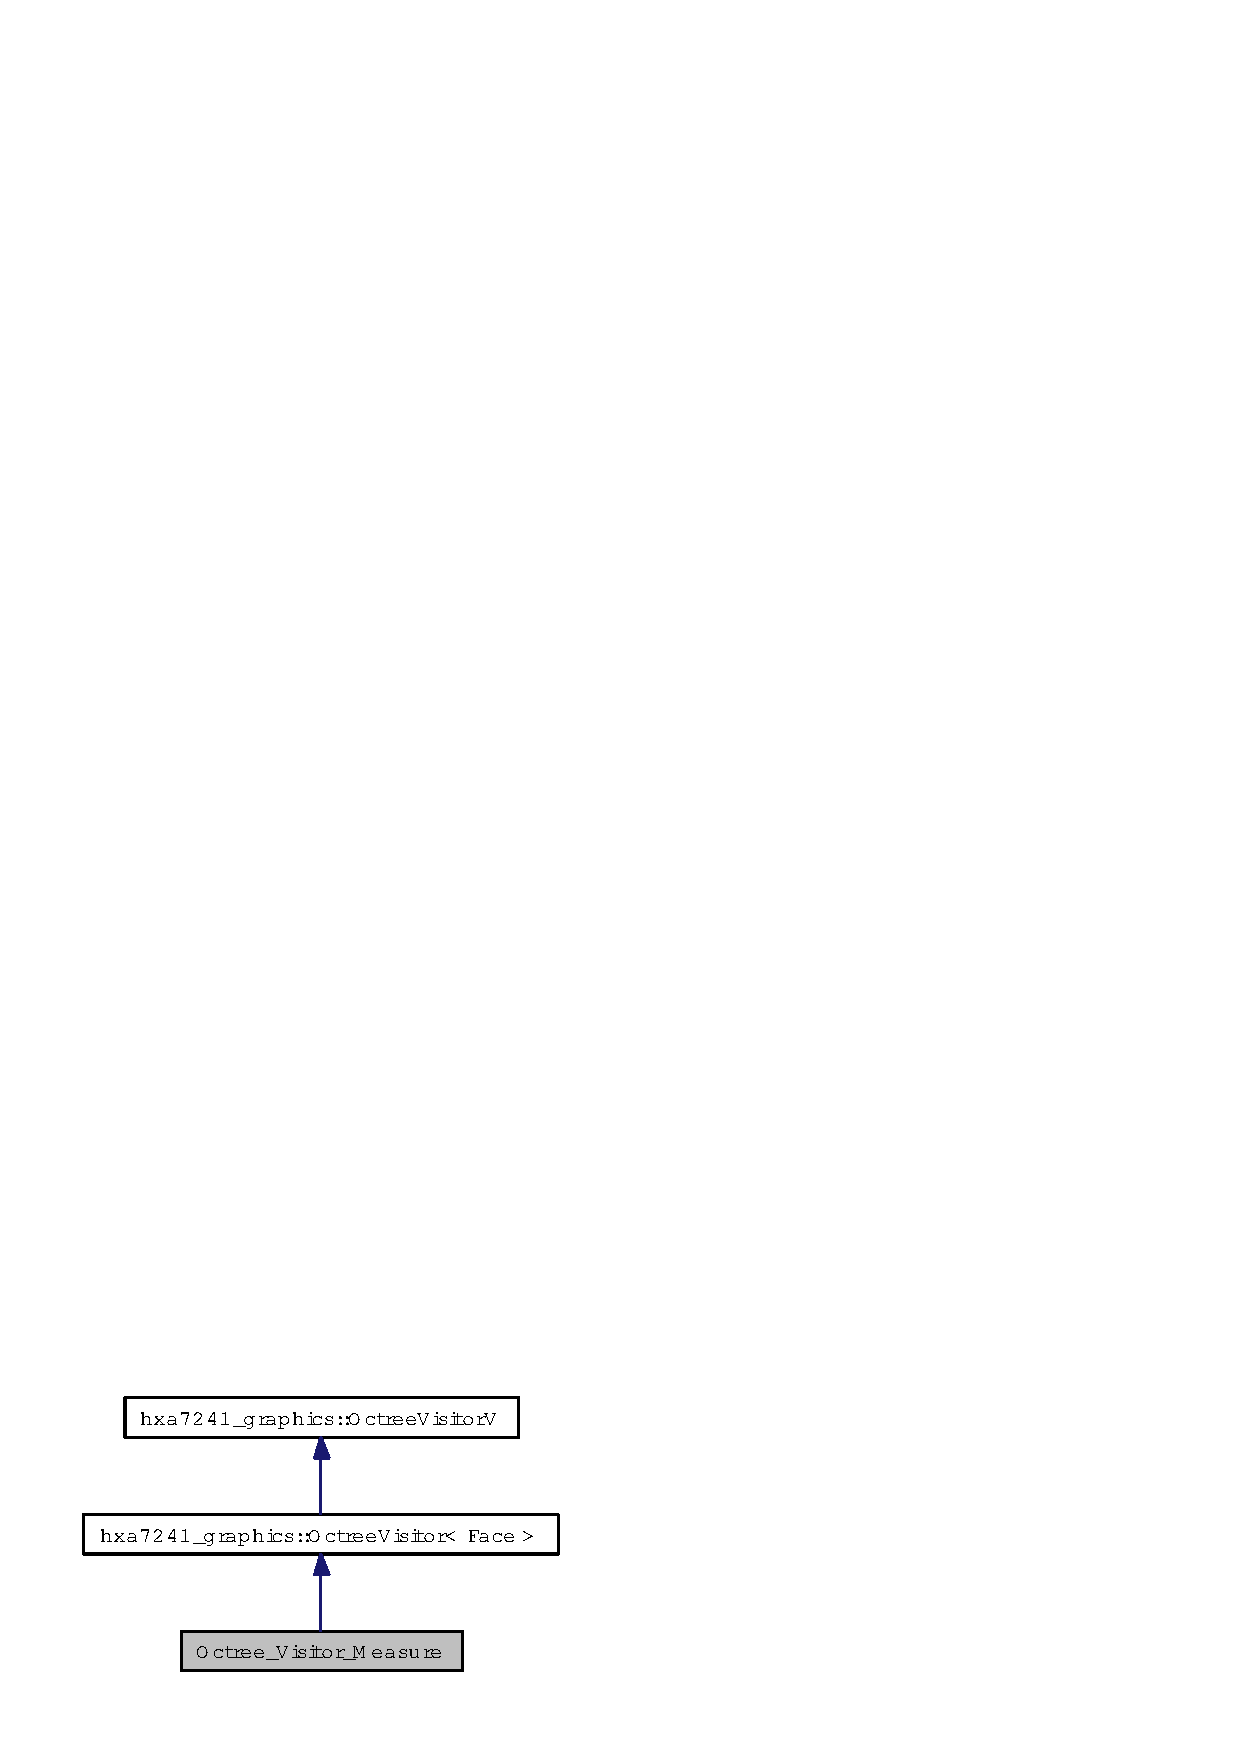
\includegraphics[width=136pt]{classOctree__Visitor__Measure__coll__graph}
\end{center}
\end{figure}
\subsection*{Public Member Functions}
\begin{CompactItemize}
\item 
{\bf Octree\_\-Visitor\_\-Measure} (void)
\begin{CompactList}\small\item\em standard object services --------------------------------------------------- \item\end{CompactList}\item 
virtual {\bf $\sim$Octree\_\-Visitor\_\-Measure} ()
\item 
int {\bf get\_\-max\_\-depth} (void)
\item 
int {\bf get\_\-num\_\-leaves} (void)
\end{CompactItemize}
\subsection*{Protected Member Functions}
\begin{CompactItemize}
\item 
virtual void {\bf visit\-Root} (const {\bf Octree\-Cell} $\ast$p\-Root\-Cell, const {\bf Octree\-Data} \&octree\-Data)
\item 
virtual void {\bf visit\-Branch} (const {\bf Octree\-Cell} $\ast$sub\-Cells[8], const {\bf Octree\-Data} \&octree\-Data)
\item 
virtual void {\bf visit\-Leaf} (const Array$<$ const {\bf Face} $\ast$ $>$ \&items, const {\bf Octree\-Data} \&octree\-Data)
\end{CompactItemize}


\subsection{Constructor \& Destructor Documentation}
\index{Octree_Visitor_Measure@{Octree\_\-Visitor\_\-Measure}!Octree_Visitor_Measure@{Octree\_\-Visitor\_\-Measure}}
\index{Octree_Visitor_Measure@{Octree\_\-Visitor\_\-Measure}!Octree_Visitor_Measure@{Octree\_\-Visitor\_\-Measure}}
\subsubsection{\setlength{\rightskip}{0pt plus 5cm}Octree\_\-Visitor\_\-Measure::Octree\_\-Visitor\_\-Measure (void)}\label{classOctree__Visitor__Measure_e865de195f510ad3100b35306b77b6a0}


standard object services --------------------------------------------------- 

\index{Octree_Visitor_Measure@{Octree\_\-Visitor\_\-Measure}!~Octree_Visitor_Measure@{$\sim$Octree\_\-Visitor\_\-Measure}}
\index{~Octree_Visitor_Measure@{$\sim$Octree\_\-Visitor\_\-Measure}!Octree_Visitor_Measure@{Octree\_\-Visitor\_\-Measure}}
\subsubsection{\setlength{\rightskip}{0pt plus 5cm}Octree\_\-Visitor\_\-Measure::$\sim$Octree\_\-Visitor\_\-Measure ()\hspace{0.3cm}{\tt  [virtual]}}\label{classOctree__Visitor__Measure_7fc195fe3e79e8ce0606031852cee598}




\subsection{Member Function Documentation}
\index{Octree_Visitor_Measure@{Octree\_\-Visitor\_\-Measure}!get_max_depth@{get\_\-max\_\-depth}}
\index{get_max_depth@{get\_\-max\_\-depth}!Octree_Visitor_Measure@{Octree\_\-Visitor\_\-Measure}}
\subsubsection{\setlength{\rightskip}{0pt plus 5cm}int Octree\_\-Visitor\_\-Measure::get\_\-max\_\-depth (void)\hspace{0.3cm}{\tt  [inline]}}\label{classOctree__Visitor__Measure_f2d9188918cf79ba8e3f8dbadbcfe805}


\index{Octree_Visitor_Measure@{Octree\_\-Visitor\_\-Measure}!get_num_leaves@{get\_\-num\_\-leaves}}
\index{get_num_leaves@{get\_\-num\_\-leaves}!Octree_Visitor_Measure@{Octree\_\-Visitor\_\-Measure}}
\subsubsection{\setlength{\rightskip}{0pt plus 5cm}int Octree\_\-Visitor\_\-Measure::get\_\-num\_\-leaves (void)\hspace{0.3cm}{\tt  [inline]}}\label{classOctree__Visitor__Measure_1def6455654fcd318c697b2a0445fe7b}


\index{Octree_Visitor_Measure@{Octree\_\-Visitor\_\-Measure}!visitRoot@{visitRoot}}
\index{visitRoot@{visitRoot}!Octree_Visitor_Measure@{Octree\_\-Visitor\_\-Measure}}
\subsubsection{\setlength{\rightskip}{0pt plus 5cm}virtual void Octree\_\-Visitor\_\-Measure::visit\-Root (const {\bf Octree\-Cell} $\ast$ {\em p\-Root\-Cell}, const {\bf Octree\-Data} \& {\em octree\-Data})\hspace{0.3cm}{\tt  [protected, virtual]}}\label{classOctree__Visitor__Measure_e12e73c31293ea5320acef16a49d14b6}


commands ------------------------------------------------------------------- octree visitor overrides 

Implements {\bf hxa7241\_\-graphics::Octree\-Visitor$<$ TYPE $>$} \doxyref{}{p.}{classhxa7241__graphics_1_1OctreeVisitor_30b2c5b03acb6c75b40d79a86e015878}.\index{Octree_Visitor_Measure@{Octree\_\-Visitor\_\-Measure}!visitBranch@{visitBranch}}
\index{visitBranch@{visitBranch}!Octree_Visitor_Measure@{Octree\_\-Visitor\_\-Measure}}
\subsubsection{\setlength{\rightskip}{0pt plus 5cm}virtual void Octree\_\-Visitor\_\-Measure::visit\-Branch (const {\bf Octree\-Cell} $\ast$ {\em sub\-Cells}[8], const {\bf Octree\-Data} \& {\em octree\-Data})\hspace{0.3cm}{\tt  [protected, virtual]}}\label{classOctree__Visitor__Measure_ab709f718cb6f6bd3d3ad4411749be04}


Called by Octree when visit traversal is at a branch.\par
\par
 To continue deeper, implementation calls Octree\-Branch::continue\-Visit( sub\-Cells, octree\-Data, sub\-Cell\-Index, $\ast$this ) for any/all sub\-Cell\-Index values. sub\-Cells elements can be null.\par
\par
 \begin{Desc}
\item[See also:]Octree\-Data \end{Desc}


Implements {\bf hxa7241\_\-graphics::Octree\-Visitor$<$ TYPE $>$} \doxyref{}{p.}{classhxa7241__graphics_1_1OctreeVisitor_e62544f5cde1e32e7fd1515e0b8d110d}.\index{Octree_Visitor_Measure@{Octree\_\-Visitor\_\-Measure}!visitLeaf@{visitLeaf}}
\index{visitLeaf@{visitLeaf}!Octree_Visitor_Measure@{Octree\_\-Visitor\_\-Measure}}
\subsubsection{\setlength{\rightskip}{0pt plus 5cm}virtual void Octree\_\-Visitor\_\-Measure::visit\-Leaf (const Array$<$ const {\bf Face} $\ast$ $>$ \& {\em items}, const {\bf Octree\-Data} \& {\em octree\-Data})\hspace{0.3cm}{\tt  [protected, virtual]}}\label{classOctree__Visitor__Measure_45a68e901c052bfc08b5e13157bf0c1b}




The documentation for this class was generated from the following files:\begin{CompactItemize}
\item 
{\bf octree\_\-visitor\_\-measure.h}\item 
{\bf octree\_\-visitor\_\-measure.cc}\end{CompactItemize}

\section{Octree\_\-Visitor\_\-Update Class Reference}
\label{classOctree__Visitor__Update}\index{Octree_Visitor_Update@{Octree\_\-Visitor\_\-Update}}
{\tt \#include $<$octree\_\-visitor\_\-update.h$>$}

Inheritance diagram for Octree\_\-Visitor\_\-Update:\begin{figure}[H]
\begin{center}
\leavevmode
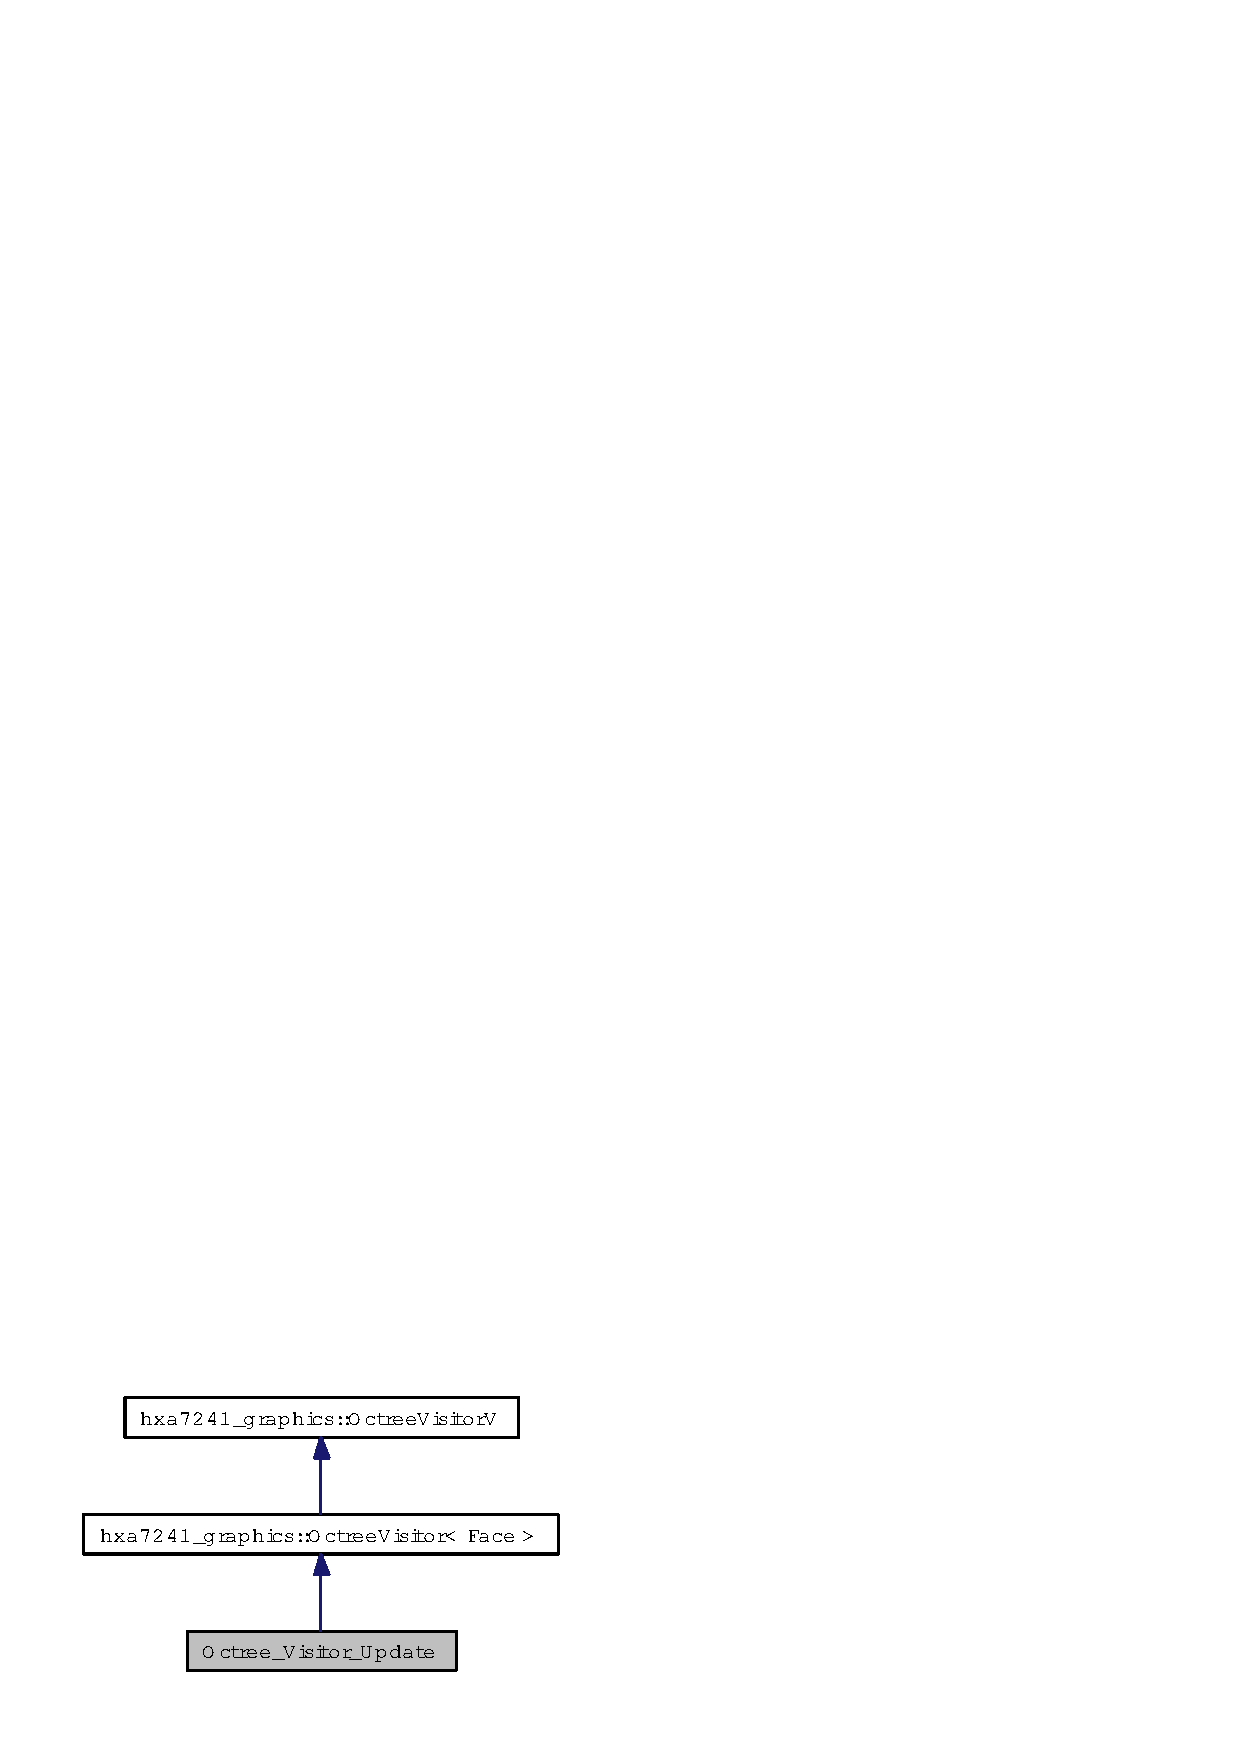
\includegraphics[width=136pt]{classOctree__Visitor__Update__inherit__graph}
\end{center}
\end{figure}
Collaboration diagram for Octree\_\-Visitor\_\-Update:\begin{figure}[H]
\begin{center}
\leavevmode
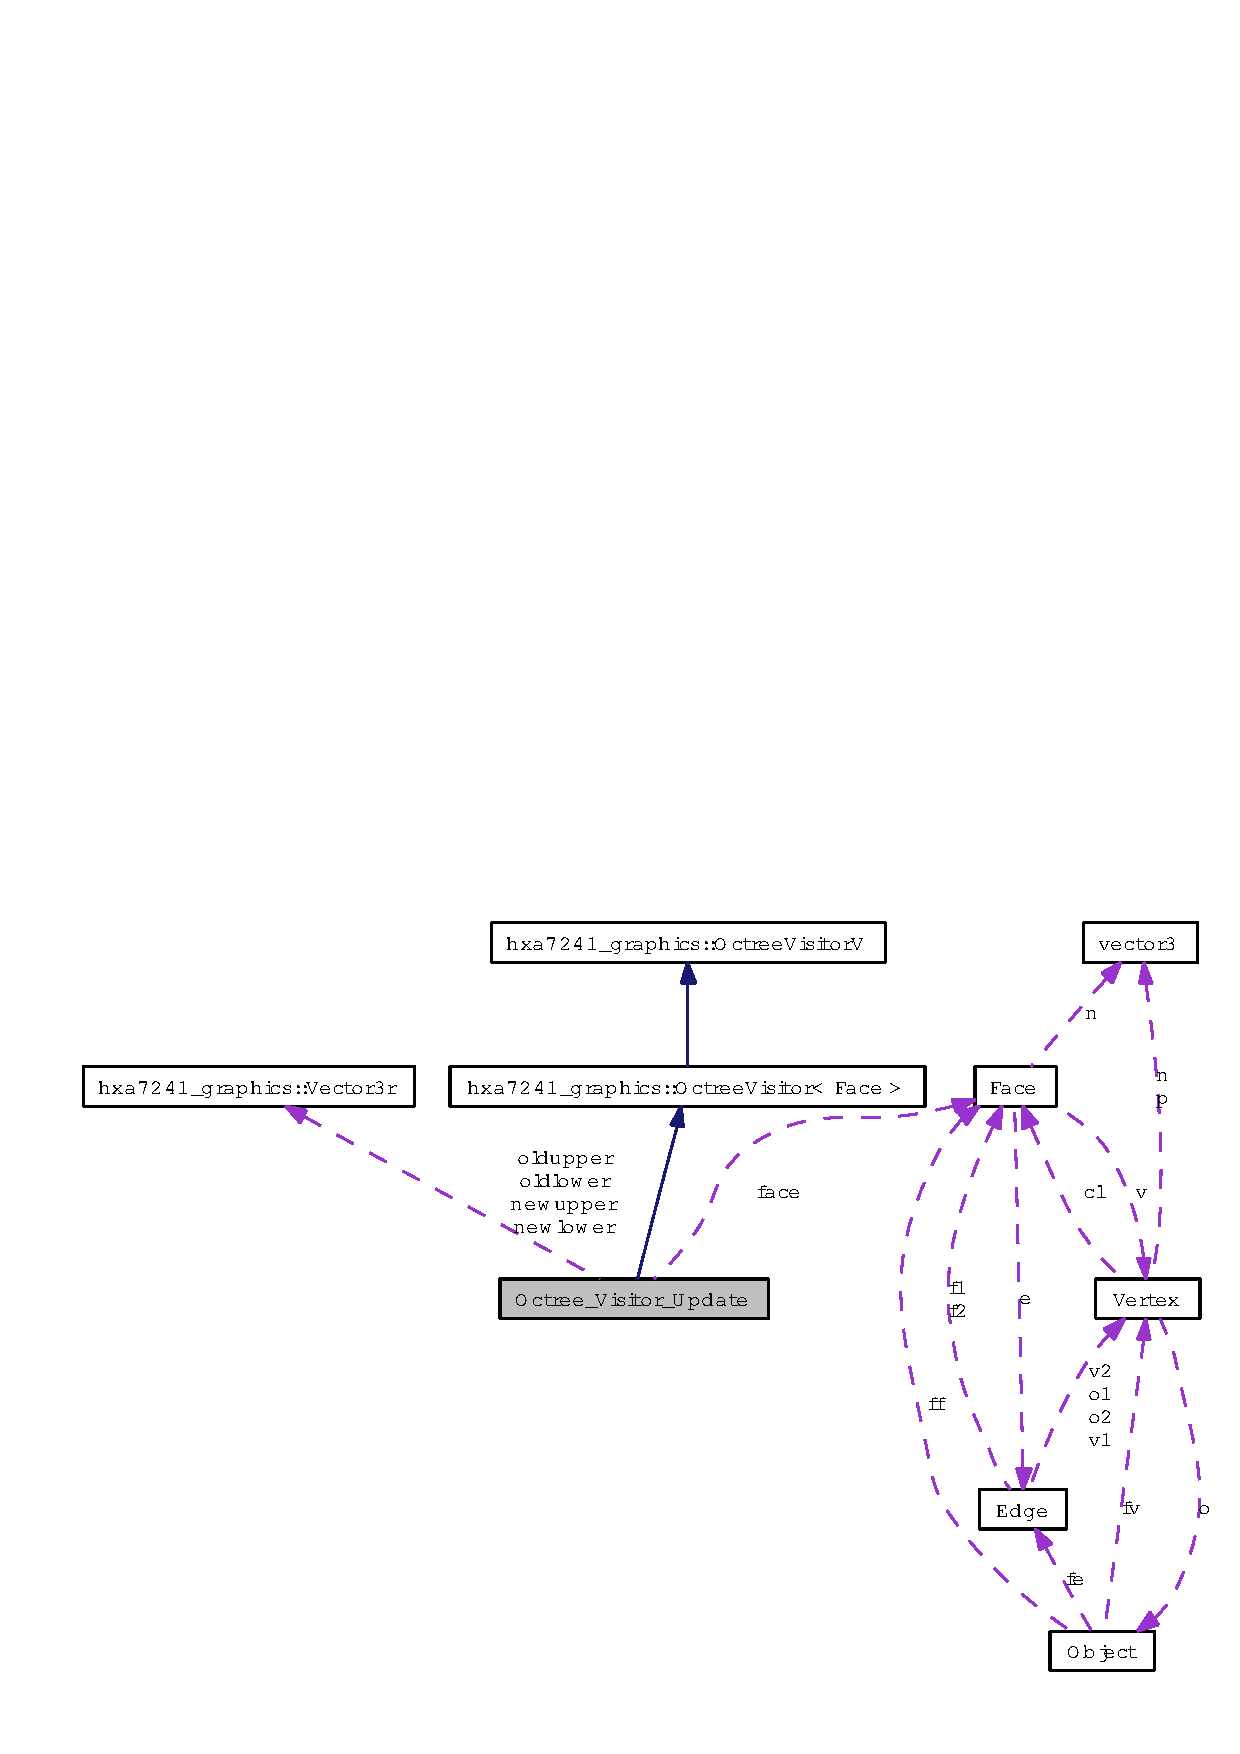
\includegraphics[width=305pt]{classOctree__Visitor__Update__coll__graph}
\end{center}
\end{figure}
\subsection*{Public Member Functions}
\begin{CompactItemize}
\item 
{\bf Octree\_\-Visitor\_\-Update} ({\bf Face} $\ast$, {\bf Vector3r}, {\bf Vector3r}, {\bf Vector3r}, {\bf Vector3r})
\begin{CompactList}\small\item\em standard object services --------------------------------------------------- \item\end{CompactList}\item 
virtual {\bf $\sim$Octree\_\-Visitor\_\-Update} ()
\end{CompactItemize}
\subsection*{Protected Member Functions}
\begin{CompactItemize}
\item 
virtual void {\bf visit\-Root} (const {\bf Octree\-Cell} $\ast$p\-Root\-Cell, const {\bf Octree\-Data} \&octree\-Data)
\item 
virtual void {\bf visit\-Branch} (const {\bf Octree\-Cell} $\ast$sub\-Cells[8], const {\bf Octree\-Data} \&octree\-Data)
\item 
virtual void {\bf visit\-Leaf} (const Array$<$ const {\bf Face} $\ast$ $>$ \&items, const {\bf Octree\-Data} \&octree\-Data)
\end{CompactItemize}


\subsection{Constructor \& Destructor Documentation}
\index{Octree_Visitor_Update@{Octree\_\-Visitor\_\-Update}!Octree_Visitor_Update@{Octree\_\-Visitor\_\-Update}}
\index{Octree_Visitor_Update@{Octree\_\-Visitor\_\-Update}!Octree_Visitor_Update@{Octree\_\-Visitor\_\-Update}}
\subsubsection{\setlength{\rightskip}{0pt plus 5cm}Octree\_\-Visitor\_\-Update::Octree\_\-Visitor\_\-Update ({\bf Face} $\ast$, {\bf Vector3r}, {\bf Vector3r}, {\bf Vector3r}, {\bf Vector3r})}\label{classOctree__Visitor__Update_7093410f63c98795f816fb60ac26adf8}


standard object services --------------------------------------------------- 

\index{Octree_Visitor_Update@{Octree\_\-Visitor\_\-Update}!~Octree_Visitor_Update@{$\sim$Octree\_\-Visitor\_\-Update}}
\index{~Octree_Visitor_Update@{$\sim$Octree\_\-Visitor\_\-Update}!Octree_Visitor_Update@{Octree\_\-Visitor\_\-Update}}
\subsubsection{\setlength{\rightskip}{0pt plus 5cm}Octree\_\-Visitor\_\-Update::$\sim$Octree\_\-Visitor\_\-Update ()\hspace{0.3cm}{\tt  [virtual]}}\label{classOctree__Visitor__Update_2b41eaf26e433332ef72ba1bd6d740f0}




\subsection{Member Function Documentation}
\index{Octree_Visitor_Update@{Octree\_\-Visitor\_\-Update}!visitRoot@{visitRoot}}
\index{visitRoot@{visitRoot}!Octree_Visitor_Update@{Octree\_\-Visitor\_\-Update}}
\subsubsection{\setlength{\rightskip}{0pt plus 5cm}virtual void Octree\_\-Visitor\_\-Update::visit\-Root (const {\bf Octree\-Cell} $\ast$ {\em p\-Root\-Cell}, const {\bf Octree\-Data} \& {\em octree\-Data})\hspace{0.3cm}{\tt  [protected, virtual]}}\label{classOctree__Visitor__Update_fc42ef265d0a074c51f403abc5dfa45f}


commands ------------------------------------------------------------------- octree visitor overrides 

Implements {\bf hxa7241\_\-graphics::Octree\-Visitor$<$ TYPE $>$} \doxyref{}{p.}{classhxa7241__graphics_1_1OctreeVisitor_30b2c5b03acb6c75b40d79a86e015878}.\index{Octree_Visitor_Update@{Octree\_\-Visitor\_\-Update}!visitBranch@{visitBranch}}
\index{visitBranch@{visitBranch}!Octree_Visitor_Update@{Octree\_\-Visitor\_\-Update}}
\subsubsection{\setlength{\rightskip}{0pt plus 5cm}virtual void Octree\_\-Visitor\_\-Update::visit\-Branch (const {\bf Octree\-Cell} $\ast$ {\em sub\-Cells}[8], const {\bf Octree\-Data} \& {\em octree\-Data})\hspace{0.3cm}{\tt  [protected, virtual]}}\label{classOctree__Visitor__Update_d9cb612bcad88d9bf13ecefc52c5f6d6}


Called by Octree when visit traversal is at a branch.\par
\par
 To continue deeper, implementation calls Octree\-Branch::continue\-Visit( sub\-Cells, octree\-Data, sub\-Cell\-Index, $\ast$this ) for any/all sub\-Cell\-Index values. sub\-Cells elements can be null.\par
\par
 \begin{Desc}
\item[See also:]Octree\-Data \end{Desc}


Implements {\bf hxa7241\_\-graphics::Octree\-Visitor$<$ TYPE $>$} \doxyref{}{p.}{classhxa7241__graphics_1_1OctreeVisitor_e62544f5cde1e32e7fd1515e0b8d110d}.\index{Octree_Visitor_Update@{Octree\_\-Visitor\_\-Update}!visitLeaf@{visitLeaf}}
\index{visitLeaf@{visitLeaf}!Octree_Visitor_Update@{Octree\_\-Visitor\_\-Update}}
\subsubsection{\setlength{\rightskip}{0pt plus 5cm}virtual void Octree\_\-Visitor\_\-Update::visit\-Leaf (const Array$<$ const {\bf Face} $\ast$ $>$ \& {\em items}, const {\bf Octree\-Data} \& {\em octree\-Data})\hspace{0.3cm}{\tt  [protected, virtual]}}\label{classOctree__Visitor__Update_e4450785e1fc3da61f53f4c5f6b1710d}




The documentation for this class was generated from the following files:\begin{CompactItemize}
\item 
{\bf octree\_\-visitor\_\-update.h}\item 
{\bf octree\_\-visitor\_\-update.cc}\end{CompactItemize}

\section{hxa7241\_\-graphics::Octree\-Agent$<$ TYPE $>$ Class Template Reference}
\label{classhxa7241__graphics_1_1OctreeAgent}\index{hxa7241_graphics::OctreeAgent@{hxa7241\_\-graphics::OctreeAgent}}
{\tt \#include $<$Octree.h$>$}

Inheritance diagram for hxa7241\_\-graphics::Octree\-Agent$<$ TYPE $>$:\begin{figure}[H]
\begin{center}
\leavevmode
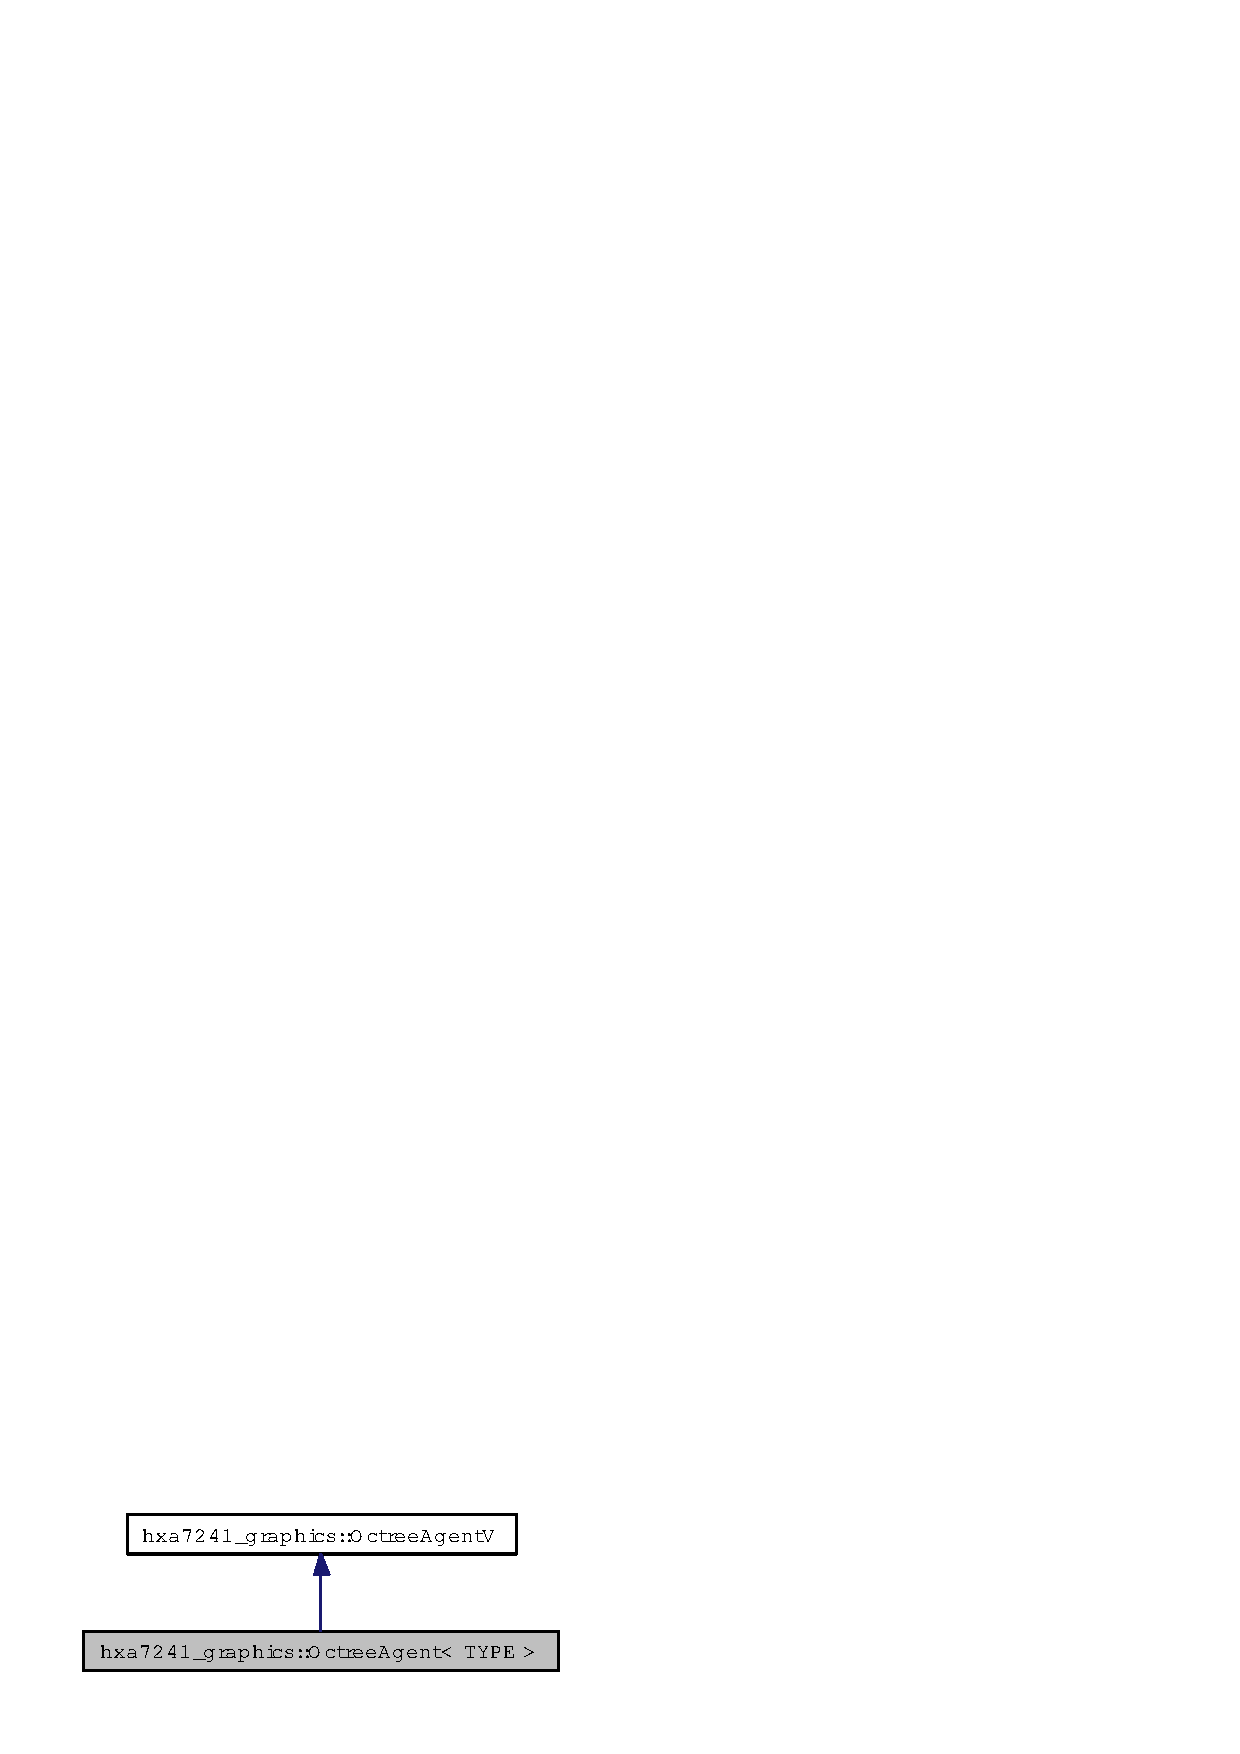
\includegraphics[width=136pt]{classhxa7241__graphics_1_1OctreeAgent__inherit__graph}
\end{center}
\end{figure}
Collaboration diagram for hxa7241\_\-graphics::Octree\-Agent$<$ TYPE $>$:\begin{figure}[H]
\begin{center}
\leavevmode
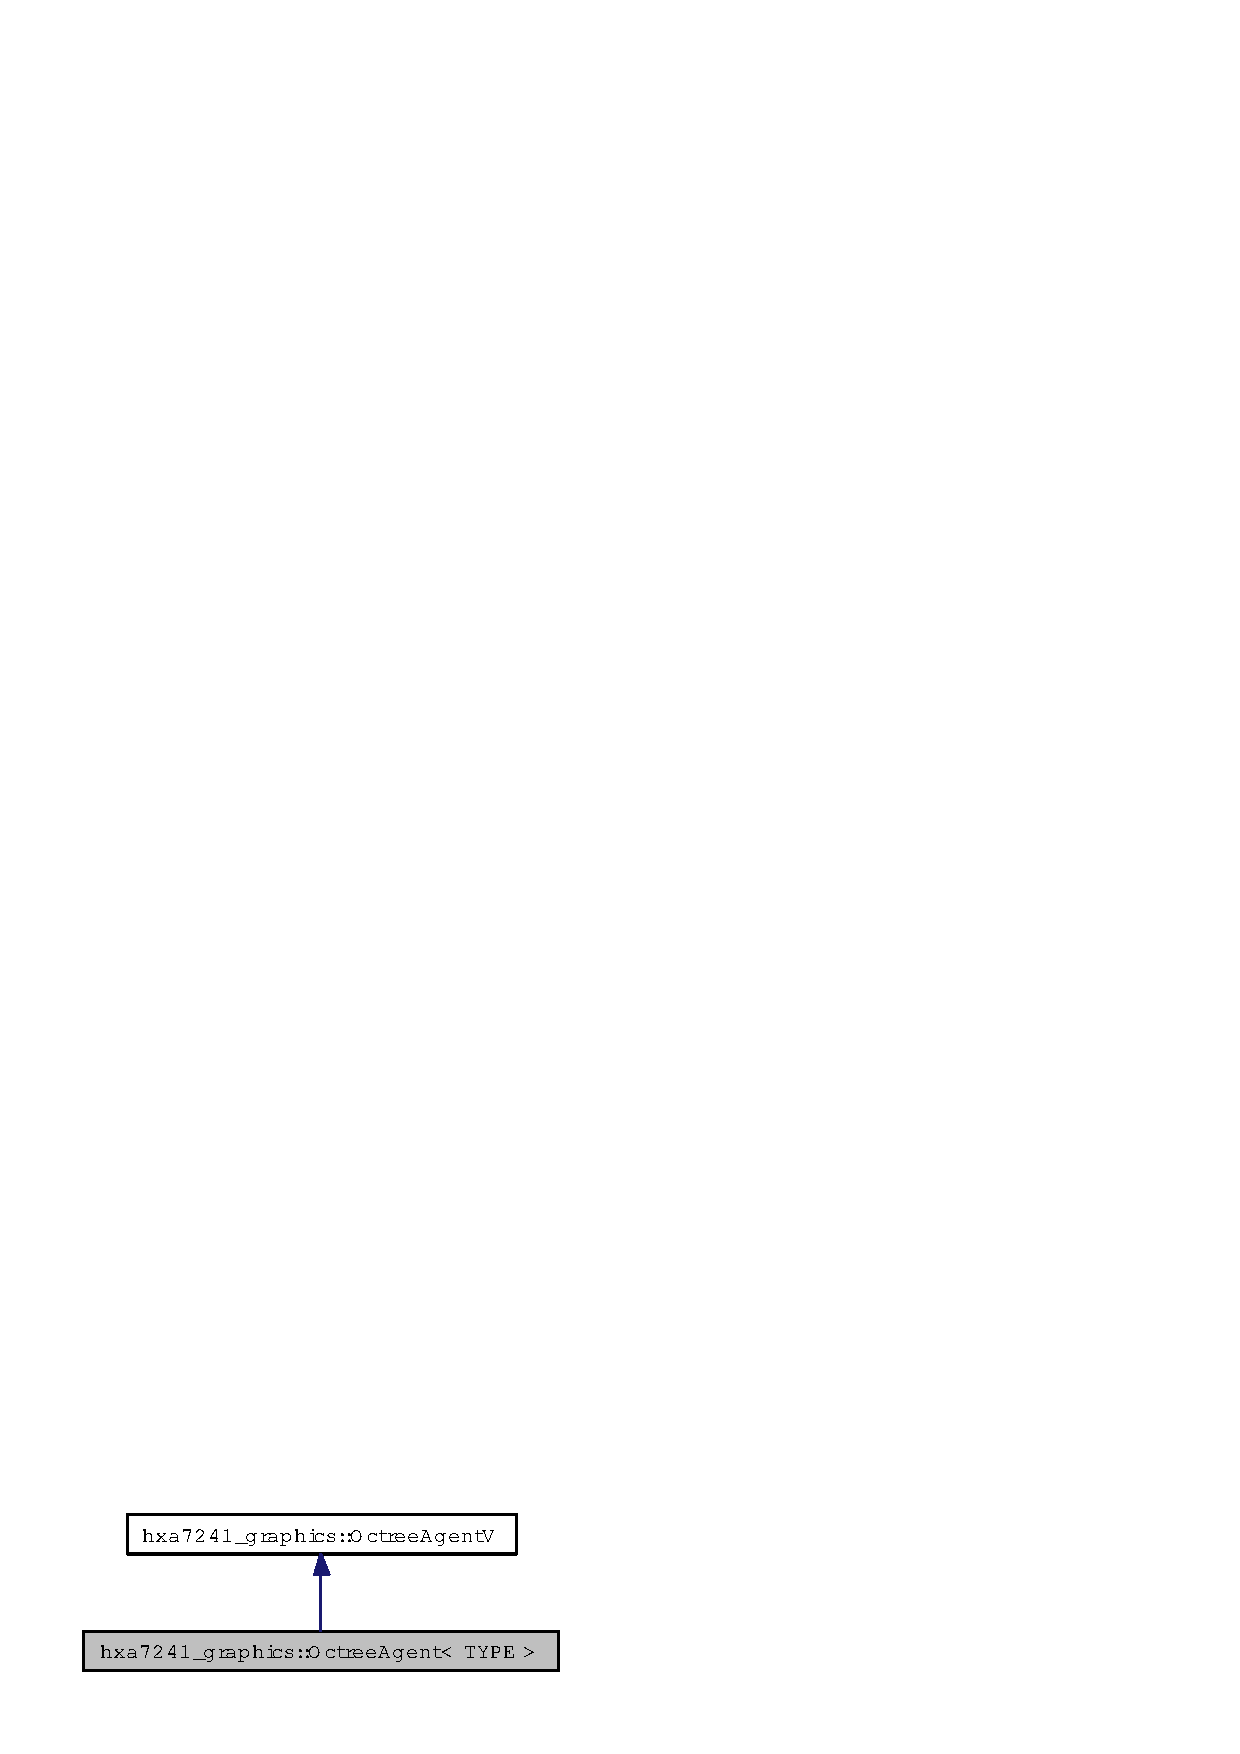
\includegraphics[width=136pt]{classhxa7241__graphics_1_1OctreeAgent__coll__graph}
\end{center}
\end{figure}
\subsection*{Public Member Functions}
\begin{CompactItemize}
\item 
virtual {\bf $\sim$Octree\-Agent} ()
\item 
virtual bool {\bf is\-Overlapping\-Cell\-V} (const void $\ast$p\-Item, const {\bf Vector3r} \&lower\-Corner, const {\bf Vector3r} \&upper\-Corner) const
\begin{CompactList}\small\item\em void-to-type forwarders \item\end{CompactList}\item 
virtual dword {\bf get\-Subcell\-Overlaps\-V} (const void $\ast$p\-Item, const {\bf Vector3r} \&lower, const {\bf Vector3r} \&middle, const {\bf Vector3r} \&upper) const
\end{CompactItemize}
\subsection*{Protected Member Functions}
\begin{CompactItemize}
\item 
{\bf Octree\-Agent} ()
\begin{CompactList}\small\item\em standard object services --------------------------------------------------- \item\end{CompactList}\item 
virtual bool {\bf is\-Overlapping\-Cell} (const TYPE \&item, const {\bf Vector3r} \&lower\-Corner, const {\bf Vector3r} \&upper\-Corner) const =0
\begin{CompactList}\small\item\em queries -------------------------------------------------------------------- \item\end{CompactList}\item 
virtual dword {\bf get\-Subcell\-Overlaps} (const TYPE \&item, const {\bf Vector3r} \&lower\-Corner, const {\bf Vector3r} \&middle\-Point, const {\bf Vector3r} \&upper\-Corner) const
\begin{CompactList}\small\item\em default implementation \item\end{CompactList}\end{CompactItemize}


\subsection{Detailed Description}
\subsubsection*{template$<$class TYPE$>$ class hxa7241\_\-graphics::Octree\-Agent$<$ TYPE $>$}

Agent abstract base, for client use with \doxyref{Octree}{p.}{classhxa7241__graphics_1_1Octree}.\par
\par


Client of \doxyref{Octree}{p.}{classhxa7241__graphics_1_1Octree} must define a concrete derivative of Octree\-Agent$<$Item\-Type$>$.\par
\par


This is similar to a proxy: it is an intermediary for an \doxyref{Octree}{p.}{classhxa7241__graphics_1_1Octree} to query its typeless subject items, when inserting or removing.\par
\par


The overlap methods are to determine an item's relation to a cell or cells, for insertion or removal. The parameters supply the bounds of the cell. \par
\par


Return value of get\-Subcell\-Overlaps is 8 bits, each bit is a bool corresponding to a subcell, the high bit for subcell 7, the low bit for subcell 0.\par
\par


Subcell numbering: \small\begin{alltt}
    y z       6 7
    |/   2 3  4 5
     -x  0 1
 \end{alltt}
\normalsize 
 in binary: \small\begin{alltt}
    y z           110 111
    |/   010 011  100 101
     -x  000 001
 \end{alltt}
\normalsize 


The \_\-\_\-\_\-V methods simply apply a type-cast to void$\ast$s and forward to their abstract counterparts.\par
\par


An \doxyref{Octree}{p.}{classhxa7241__graphics_1_1Octree} requires its contained items to provide positional info. But requiring the item classes to implement an Octree\-Item interface would impose a direct interface change on every prospective item type, and enlarge their instances with a vptr.\par
\par


Instead, this agent transfers the Octree-related interface/implementation away from the item type into a separate class. The \doxyref{Octree}{p.}{classhxa7241__graphics_1_1Octree} can now hold void pointers to items and call the agent to query them indirectly.\par
\par
 



\subsection{Constructor \& Destructor Documentation}
\index{hxa7241_graphics::OctreeAgent@{hxa7241\_\-graphics::Octree\-Agent}!OctreeAgent@{OctreeAgent}}
\index{OctreeAgent@{OctreeAgent}!hxa7241_graphics::OctreeAgent@{hxa7241\_\-graphics::Octree\-Agent}}
\subsubsection{\setlength{\rightskip}{0pt plus 5cm}template$<$class TYPE$>$ {\bf hxa7241\_\-graphics::Octree\-Agent}$<$ TYPE $>$::{\bf Octree\-Agent} ()\hspace{0.3cm}{\tt  [inline, protected]}}\label{classhxa7241__graphics_1_1OctreeAgent_77f0b8bc444f3cc58d2487e657123545}


standard object services --------------------------------------------------- 

\index{hxa7241_graphics::OctreeAgent@{hxa7241\_\-graphics::Octree\-Agent}!~OctreeAgent@{$\sim$OctreeAgent}}
\index{~OctreeAgent@{$\sim$OctreeAgent}!hxa7241_graphics::OctreeAgent@{hxa7241\_\-graphics::Octree\-Agent}}
\subsubsection{\setlength{\rightskip}{0pt plus 5cm}template$<$class TYPE$>$ virtual {\bf hxa7241\_\-graphics::Octree\-Agent}$<$ TYPE $>$::$\sim${\bf Octree\-Agent} ()\hspace{0.3cm}{\tt  [inline, virtual]}}\label{classhxa7241__graphics_1_1OctreeAgent_60870fa6b28b3e263189809cb493cfc4}




\subsection{Member Function Documentation}
\index{hxa7241_graphics::OctreeAgent@{hxa7241\_\-graphics::Octree\-Agent}!isOverlappingCellV@{isOverlappingCellV}}
\index{isOverlappingCellV@{isOverlappingCellV}!hxa7241_graphics::OctreeAgent@{hxa7241\_\-graphics::Octree\-Agent}}
\subsubsection{\setlength{\rightskip}{0pt plus 5cm}template$<$class TYPE$>$ bool {\bf hxa7241\_\-graphics::Octree\-Agent}$<$ TYPE $>$::is\-Overlapping\-Cell\-V (const void $\ast$ {\em p\-Item}, const {\bf Vector3r} \& {\em lower\-Corner}, const {\bf Vector3r} \& {\em upper\-Corner}) const\hspace{0.3cm}{\tt  [inline, virtual]}}\label{classhxa7241__graphics_1_1OctreeAgent_2640e4adca884dc4531a93215ef9f75c}


void-to-type forwarders 



Implements {\bf hxa7241\_\-graphics::Octree\-Agent\-V} \doxyref{}{p.}{classhxa7241__graphics_1_1OctreeAgentV_25a8bdfe6e2bfcc9dc307c22915a32ef}.\index{hxa7241_graphics::OctreeAgent@{hxa7241\_\-graphics::Octree\-Agent}!getSubcellOverlapsV@{getSubcellOverlapsV}}
\index{getSubcellOverlapsV@{getSubcellOverlapsV}!hxa7241_graphics::OctreeAgent@{hxa7241\_\-graphics::Octree\-Agent}}
\subsubsection{\setlength{\rightskip}{0pt plus 5cm}template$<$class TYPE$>$ dword {\bf hxa7241\_\-graphics::Octree\-Agent}$<$ TYPE $>$::get\-Subcell\-Overlaps\-V (const void $\ast$ {\em p\-Item}, const {\bf Vector3r} \& {\em lower}, const {\bf Vector3r} \& {\em middle}, const {\bf Vector3r} \& {\em upper}) const\hspace{0.3cm}{\tt  [inline, virtual]}}\label{classhxa7241__graphics_1_1OctreeAgent_1f3c0ce8e9f03e52de13262e095a2968}




Implements {\bf hxa7241\_\-graphics::Octree\-Agent\-V} \doxyref{}{p.}{classhxa7241__graphics_1_1OctreeAgentV_219e72c02f6845a5802349ef6d8bf115}.\index{hxa7241_graphics::OctreeAgent@{hxa7241\_\-graphics::Octree\-Agent}!isOverlappingCell@{isOverlappingCell}}
\index{isOverlappingCell@{isOverlappingCell}!hxa7241_graphics::OctreeAgent@{hxa7241\_\-graphics::Octree\-Agent}}
\subsubsection{\setlength{\rightskip}{0pt plus 5cm}template$<$class TYPE$>$ virtual bool {\bf hxa7241\_\-graphics::Octree\-Agent}$<$ TYPE $>$::is\-Overlapping\-Cell (const TYPE \& {\em item}, const {\bf Vector3r} \& {\em lower\-Corner}, const {\bf Vector3r} \& {\em upper\-Corner}) const\hspace{0.3cm}{\tt  [protected, pure virtual]}}\label{classhxa7241__graphics_1_1OctreeAgent_a2df3912d793763643522ffd2f451dbb}


queries -------------------------------------------------------------------- 

Called by \doxyref{Octree}{p.}{classhxa7241__graphics_1_1Octree} to get relation of item to cell. 

Implemented in {\bf Octree\_\-Agent\_\-Face} \doxyref{}{p.}{classOctree__Agent__Face_1fc918ffe7dee3ca4f6a9ccd47f98000}.\index{hxa7241_graphics::OctreeAgent@{hxa7241\_\-graphics::Octree\-Agent}!getSubcellOverlaps@{getSubcellOverlaps}}
\index{getSubcellOverlaps@{getSubcellOverlaps}!hxa7241_graphics::OctreeAgent@{hxa7241\_\-graphics::Octree\-Agent}}
\subsubsection{\setlength{\rightskip}{0pt plus 5cm}template$<$class TYPE$>$ dword {\bf hxa7241\_\-graphics::Octree\-Agent}$<$ TYPE $>$::get\-Subcell\-Overlaps (const TYPE \& {\em item}, const {\bf Vector3r} \& {\em lower\-Corner}, const {\bf Vector3r} \& {\em middle\-Point}, const {\bf Vector3r} \& {\em upper\-Corner}) const\hspace{0.3cm}{\tt  [protected, virtual]}}\label{classhxa7241__graphics_1_1OctreeAgent_c9c3473ff6749775aa199998de0bdcf6}


default implementation 

Called by \doxyref{Octree}{p.}{classhxa7241__graphics_1_1Octree} to get relation of item to subcell octants.\par
\par
 Override to make a more efficent calculation (boundary testing can be shared). \begin{Desc}
\item[Returns:]8 bits, each a bool corresponding to a subcell, the high bit for subcell 7, the low bit for subcell 0.\par
\par
 Subcell numbering: \small\begin{alltt}
    y z       6 7
    |/   2 3  4 5
     -x  0 1
 \end{alltt}
\normalsize 
 in binary: \small\begin{alltt}
    y z           110 111
    |/   010 011  100 101
     -x  000 001
 \end{alltt}
\normalsize 
 \end{Desc}


The documentation for this class was generated from the following file:\begin{CompactItemize}
\item 
{\bf Octree.h}\end{CompactItemize}

\section{hxa7241\_\-graphics::Octree\-Agent\-V Class Reference}
\label{classhxa7241__graphics_1_1OctreeAgentV}\index{hxa7241_graphics::OctreeAgentV@{hxa7241\_\-graphics::OctreeAgentV}}
{\tt \#include $<$Octree\-Auxiliary.h$>$}

Inheritance diagram for hxa7241\_\-graphics::Octree\-Agent\-V:\begin{figure}[H]
\begin{center}
\leavevmode
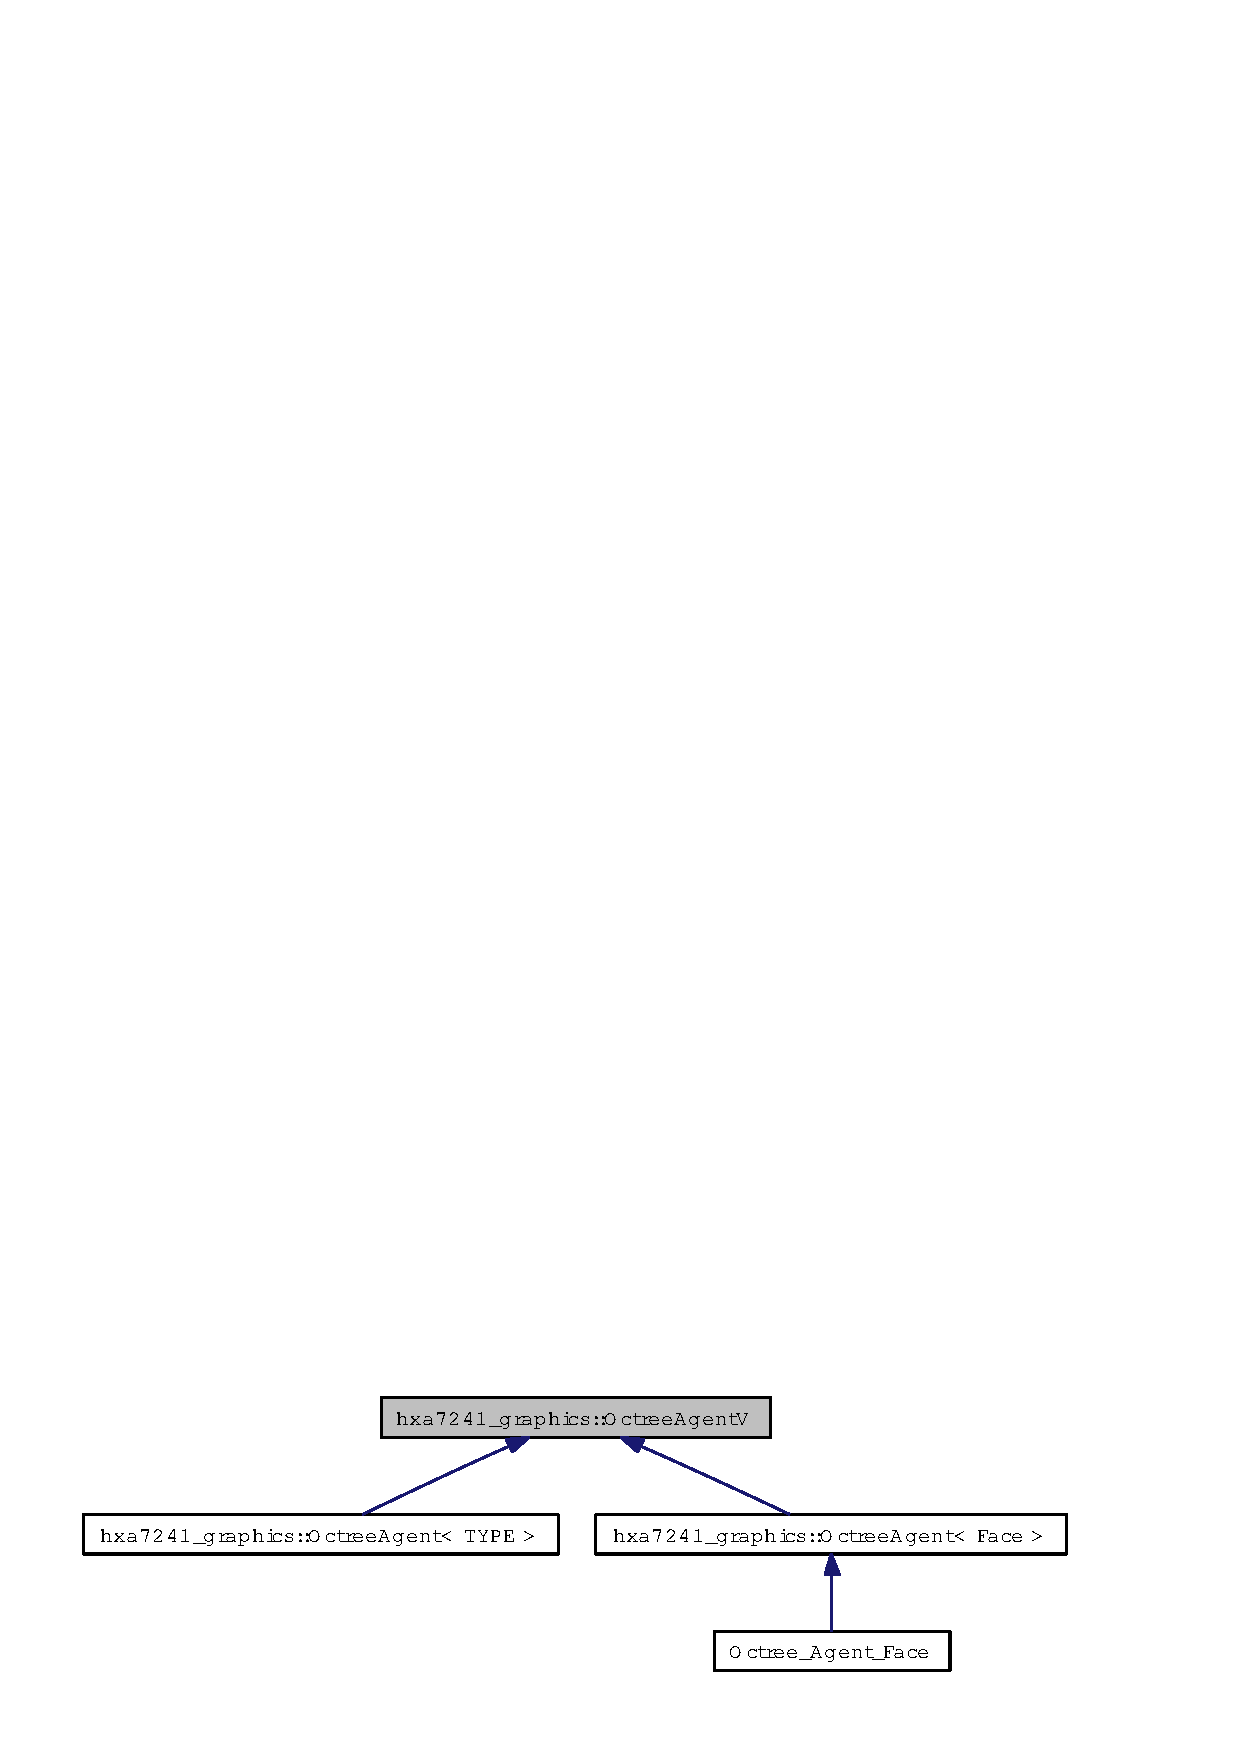
\includegraphics[width=258pt]{classhxa7241__graphics_1_1OctreeAgentV__inherit__graph}
\end{center}
\end{figure}
\subsection*{Public Member Functions}
\begin{CompactItemize}
\item 
virtual {\bf $\sim$Octree\-Agent\-V} ()
\item 
virtual bool {\bf is\-Overlapping\-Cell\-V} (const void $\ast$p\-Item, const {\bf Vector3r} \&lower\-Corner, const {\bf Vector3r} \&upper\-Corner) const=0
\begin{CompactList}\small\item\em queries -------------------------------------------------------------------- \item\end{CompactList}\item 
virtual dword {\bf get\-Subcell\-Overlaps\-V} (const void $\ast$p\-Item, const {\bf Vector3r} \&lower, const {\bf Vector3r} \&middle, const {\bf Vector3r} \&upper) const=0
\end{CompactItemize}
\subsection*{Static Public Attributes}
\begin{CompactItemize}
\item 
static const dword {\bf ALL\_\-INSIDE} = 0x0000FFFF
\begin{CompactList}\small\item\em constants ------------------------------------------------------------------ \item\end{CompactList}\item 
static const dword {\bf ALL\_\-OUTSIDE} = 0x00000000
\end{CompactItemize}
\subsection*{Protected Member Functions}
\begin{CompactItemize}
\item 
{\bf Octree\-Agent\-V} ()
\begin{CompactList}\small\item\em standard object services --------------------------------------------------- \item\end{CompactList}\end{CompactItemize}


\subsection{Detailed Description}
Agent abstract base, for \doxyref{Octree}{p.}{classhxa7241__graphics_1_1Octree} implementation use.\par
\par


Return value of get\-Subcell\-Overlaps\-V is 8 bits, each bit is a bool corresponding to a subcell, the high bit for subcell 7, the low bit for subcell 0.\par
\par


Subcell numbering: \small\begin{alltt}
    y z       6 7
    |/   2 3  4 5
     -x  0 1
 \end{alltt}
\normalsize 
 in binary: \small\begin{alltt}
    y z           110 111
    |/   010 011  100 101
     -x  000 001
 \end{alltt}
\normalsize 


\begin{Desc}
\item[See also:]\doxyref{Octree\-Cell}{p.}{classhxa7241__graphics_1_1OctreeCell} 

\doxyref{Octree\-Branch}{p.}{classhxa7241__graphics_1_1OctreeBranch} 

\doxyref{Octree\-Leaf}{p.}{classhxa7241__graphics_1_1OctreeLeaf} \end{Desc}




\subsection{Constructor \& Destructor Documentation}
\index{hxa7241_graphics::OctreeAgentV@{hxa7241\_\-graphics::Octree\-Agent\-V}!OctreeAgentV@{OctreeAgentV}}
\index{OctreeAgentV@{OctreeAgentV}!hxa7241_graphics::OctreeAgentV@{hxa7241\_\-graphics::Octree\-Agent\-V}}
\subsubsection{\setlength{\rightskip}{0pt plus 5cm}hxa7241\_\-graphics::Octree\-Agent\-V::Octree\-Agent\-V ()\hspace{0.3cm}{\tt  [inline, protected]}}\label{classhxa7241__graphics_1_1OctreeAgentV_19043bdcd8c7e685c032db8ef5bb8316}


standard object services --------------------------------------------------- 

\index{hxa7241_graphics::OctreeAgentV@{hxa7241\_\-graphics::Octree\-Agent\-V}!~OctreeAgentV@{$\sim$OctreeAgentV}}
\index{~OctreeAgentV@{$\sim$OctreeAgentV}!hxa7241_graphics::OctreeAgentV@{hxa7241\_\-graphics::Octree\-Agent\-V}}
\subsubsection{\setlength{\rightskip}{0pt plus 5cm}virtual hxa7241\_\-graphics::Octree\-Agent\-V::$\sim$Octree\-Agent\-V ()\hspace{0.3cm}{\tt  [inline, virtual]}}\label{classhxa7241__graphics_1_1OctreeAgentV_5f96881e48a77c3157e4e0fcc3249c56}




\subsection{Member Function Documentation}
\index{hxa7241_graphics::OctreeAgentV@{hxa7241\_\-graphics::Octree\-Agent\-V}!isOverlappingCellV@{isOverlappingCellV}}
\index{isOverlappingCellV@{isOverlappingCellV}!hxa7241_graphics::OctreeAgentV@{hxa7241\_\-graphics::Octree\-Agent\-V}}
\subsubsection{\setlength{\rightskip}{0pt plus 5cm}virtual bool hxa7241\_\-graphics::Octree\-Agent\-V::is\-Overlapping\-Cell\-V (const void $\ast$ {\em p\-Item}, const {\bf Vector3r} \& {\em lower\-Corner}, const {\bf Vector3r} \& {\em upper\-Corner}) const\hspace{0.3cm}{\tt  [pure virtual]}}\label{classhxa7241__graphics_1_1OctreeAgentV_25a8bdfe6e2bfcc9dc307c22915a32ef}


queries -------------------------------------------------------------------- 



Implemented in {\bf hxa7241\_\-graphics::Octree\-Agent$<$ TYPE $>$} \doxyref{}{p.}{classhxa7241__graphics_1_1OctreeAgent_2640e4adca884dc4531a93215ef9f75c}, and {\bf hxa7241\_\-graphics::Octree\-Agent$<$ Face $>$} \doxyref{}{p.}{classhxa7241__graphics_1_1OctreeAgent_2640e4adca884dc4531a93215ef9f75c}.\index{hxa7241_graphics::OctreeAgentV@{hxa7241\_\-graphics::Octree\-Agent\-V}!getSubcellOverlapsV@{getSubcellOverlapsV}}
\index{getSubcellOverlapsV@{getSubcellOverlapsV}!hxa7241_graphics::OctreeAgentV@{hxa7241\_\-graphics::Octree\-Agent\-V}}
\subsubsection{\setlength{\rightskip}{0pt plus 5cm}virtual dword hxa7241\_\-graphics::Octree\-Agent\-V::get\-Subcell\-Overlaps\-V (const void $\ast$ {\em p\-Item}, const {\bf Vector3r} \& {\em lower}, const {\bf Vector3r} \& {\em middle}, const {\bf Vector3r} \& {\em upper}) const\hspace{0.3cm}{\tt  [pure virtual]}}\label{classhxa7241__graphics_1_1OctreeAgentV_219e72c02f6845a5802349ef6d8bf115}




Implemented in {\bf hxa7241\_\-graphics::Octree\-Agent$<$ TYPE $>$} \doxyref{}{p.}{classhxa7241__graphics_1_1OctreeAgent_1f3c0ce8e9f03e52de13262e095a2968}, and {\bf hxa7241\_\-graphics::Octree\-Agent$<$ Face $>$} \doxyref{}{p.}{classhxa7241__graphics_1_1OctreeAgent_1f3c0ce8e9f03e52de13262e095a2968}.

\subsection{Member Data Documentation}
\index{hxa7241_graphics::OctreeAgentV@{hxa7241\_\-graphics::Octree\-Agent\-V}!ALL_INSIDE@{ALL\_\-INSIDE}}
\index{ALL_INSIDE@{ALL\_\-INSIDE}!hxa7241_graphics::OctreeAgentV@{hxa7241\_\-graphics::Octree\-Agent\-V}}
\subsubsection{\setlength{\rightskip}{0pt plus 5cm}const dword {\bf hxa7241\_\-graphics::Octree\-Agent\-V::ALL\_\-INSIDE} = 0x0000FFFF\hspace{0.3cm}{\tt  [static]}}\label{classhxa7241__graphics_1_1OctreeAgentV_575e0cac525016eca33639630683230c}


constants ------------------------------------------------------------------ 

\index{hxa7241_graphics::OctreeAgentV@{hxa7241\_\-graphics::Octree\-Agent\-V}!ALL_OUTSIDE@{ALL\_\-OUTSIDE}}
\index{ALL_OUTSIDE@{ALL\_\-OUTSIDE}!hxa7241_graphics::OctreeAgentV@{hxa7241\_\-graphics::Octree\-Agent\-V}}
\subsubsection{\setlength{\rightskip}{0pt plus 5cm}const dword {\bf hxa7241\_\-graphics::Octree\-Agent\-V::ALL\_\-OUTSIDE} = 0x00000000\hspace{0.3cm}{\tt  [static]}}\label{classhxa7241__graphics_1_1OctreeAgentV_44d70782aaf6ad8eefc46d41efb93d44}




The documentation for this class was generated from the following file:\begin{CompactItemize}
\item 
{\bf Octree\-Auxiliary.h}\end{CompactItemize}

\section{hxa7241\_\-graphics::Octree\-Bound Class Reference}
\label{classhxa7241__graphics_1_1OctreeBound}\index{hxa7241_graphics::OctreeBound@{hxa7241\_\-graphics::OctreeBound}}
{\tt \#include $<$Octree\-Auxiliary.h$>$}

Collaboration diagram for hxa7241\_\-graphics::Octree\-Bound:\begin{figure}[H]
\begin{center}
\leavevmode
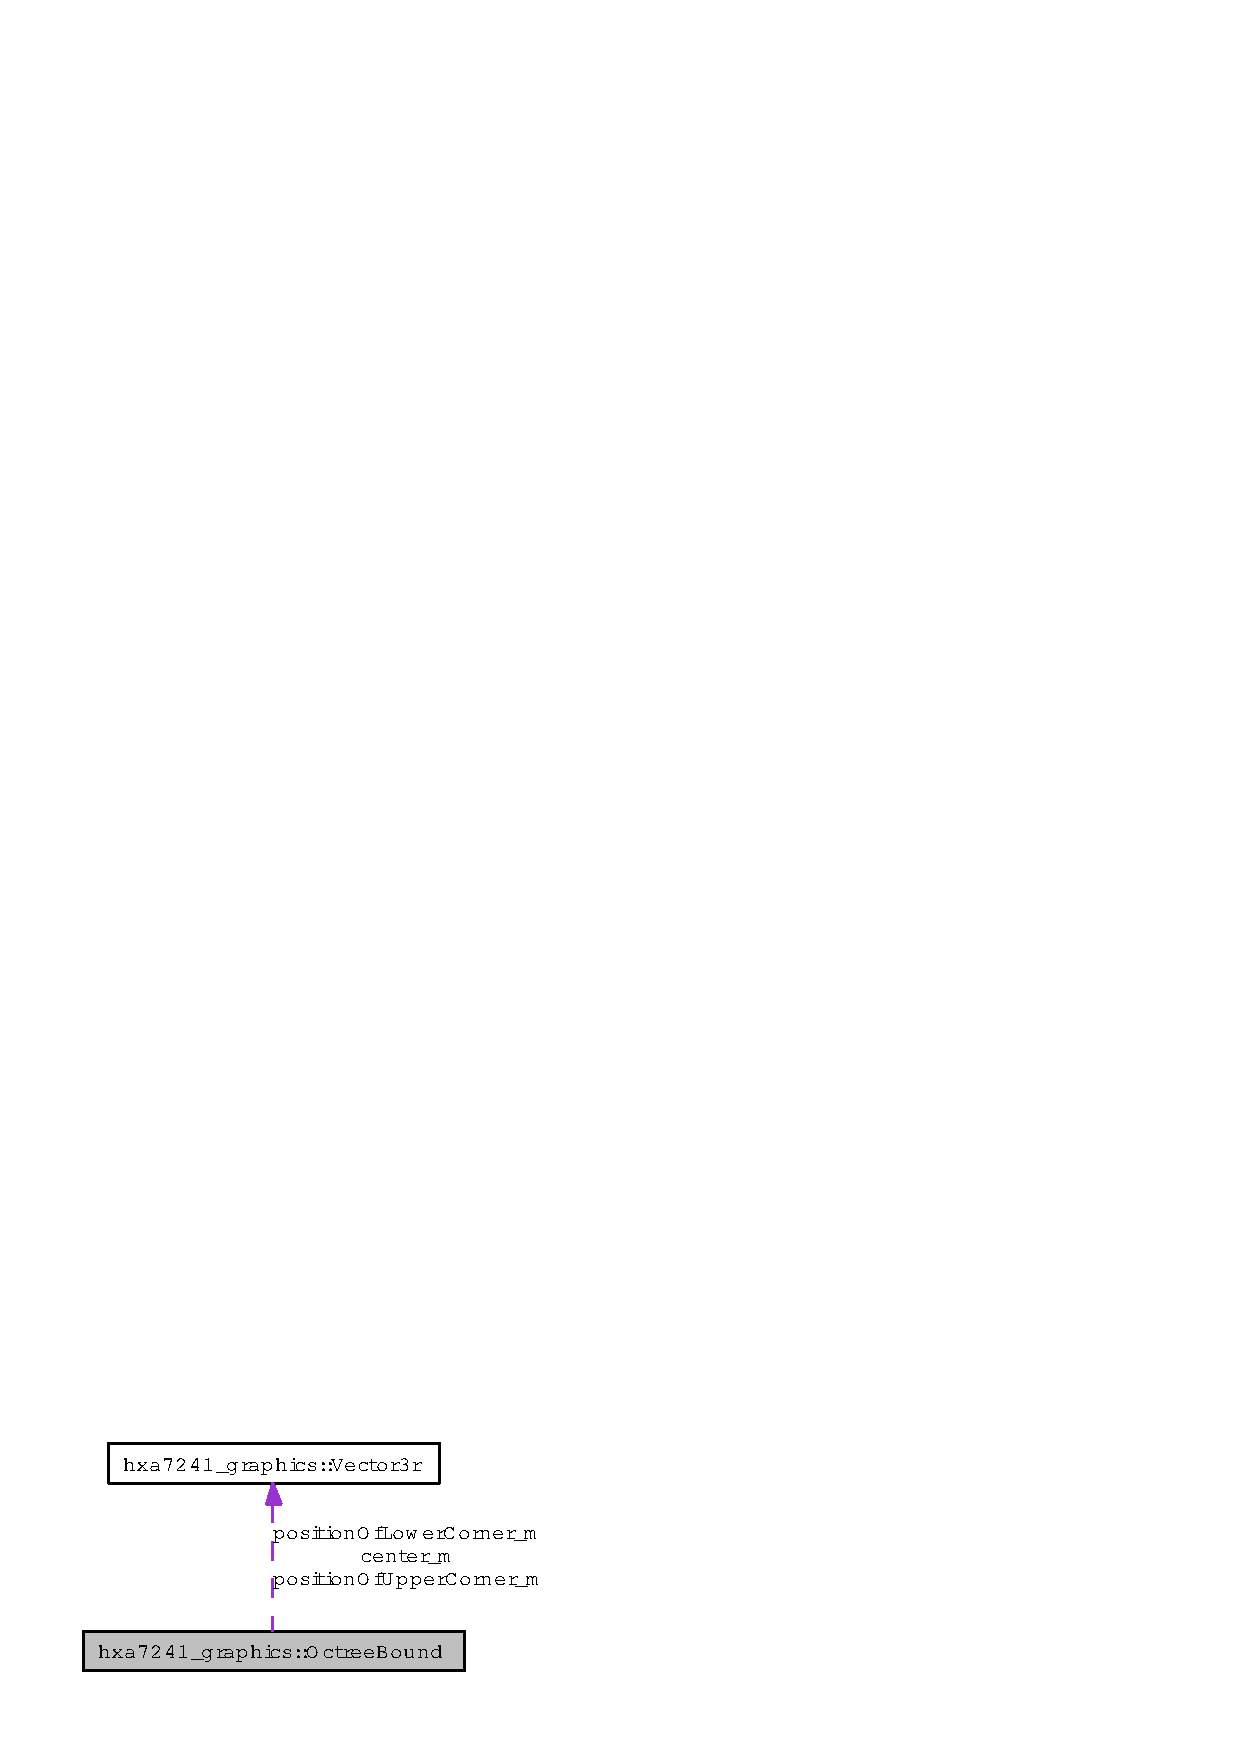
\includegraphics[width=133pt]{classhxa7241__graphics_1_1OctreeBound__coll__graph}
\end{center}
\end{figure}
\subsection*{Public Member Functions}
\begin{CompactItemize}
\item 
{\bf Octree\-Bound} ()
\begin{CompactList}\small\item\em standard object services --------------------------------------------------- \item\end{CompactList}\item 
{\bf Octree\-Bound} (const {\bf Vector3r} \&position\-Of\-Lower\-Corner, real size)
\item 
{\bf Octree\-Bound} (const {\bf Octree\-Bound} \&parent\-Cell\-Bound, dword sub\-Cell\-Index)
\item 
{\bf $\sim$Octree\-Bound} ()
\item 
{\bf Octree\-Bound} (const {\bf Octree\-Bound} \&)
\item 
{\bf Octree\-Bound} \& {\bf operator=} (const {\bf Octree\-Bound} \&)
\item 
const {\bf Vector3r} \& {\bf get\-Lower\-Corner} () const
\begin{CompactList}\small\item\em \doxyref{Octree\-Bound}{p.}{classhxa7241__graphics_1_1OctreeBound} ----------------------------------------------------------------. \item\end{CompactList}\item 
const {\bf Vector3r} \& {\bf get\-Upper\-Corner} () const
\item 
const {\bf Vector3r} \& {\bf get\-Center} () const
\item 
real {\bf get\-Radius} () const
\item 
real {\bf get\-Size} () const
\end{CompactItemize}


\subsection{Detailed Description}
Geometric data for the bound of an octree cell.\par
\par


Constant.\par
\par


Radius is that of the circumsphere.\par
\par


Subcell numbering: \small\begin{alltt}
    y z       6 7
    |/   2 3  4 5
     -x  0 1
 \end{alltt}
\normalsize 
 in binary: \small\begin{alltt}
    y z           110 111
    |/   010 011  100 101
     -x  000 001
 \end{alltt}
\normalsize 
 



\subsection{Constructor \& Destructor Documentation}
\index{hxa7241_graphics::OctreeBound@{hxa7241\_\-graphics::Octree\-Bound}!OctreeBound@{OctreeBound}}
\index{OctreeBound@{OctreeBound}!hxa7241_graphics::OctreeBound@{hxa7241\_\-graphics::Octree\-Bound}}
\subsubsection{\setlength{\rightskip}{0pt plus 5cm}Octree\-Bound::Octree\-Bound ()}\label{classhxa7241__graphics_1_1OctreeBound_104e42dc39b274fecda123f95c0dcf91}


standard object services --------------------------------------------------- 

\index{hxa7241_graphics::OctreeBound@{hxa7241\_\-graphics::Octree\-Bound}!OctreeBound@{OctreeBound}}
\index{OctreeBound@{OctreeBound}!hxa7241_graphics::OctreeBound@{hxa7241\_\-graphics::Octree\-Bound}}
\subsubsection{\setlength{\rightskip}{0pt plus 5cm}Octree\-Bound::Octree\-Bound (const {\bf Vector3r} \& {\em position\-Of\-Lower\-Corner}, real {\em size})}\label{classhxa7241__graphics_1_1OctreeBound_82bf086c05629a8a92808a3c612e9772}


\index{hxa7241_graphics::OctreeBound@{hxa7241\_\-graphics::Octree\-Bound}!OctreeBound@{OctreeBound}}
\index{OctreeBound@{OctreeBound}!hxa7241_graphics::OctreeBound@{hxa7241\_\-graphics::Octree\-Bound}}
\subsubsection{\setlength{\rightskip}{0pt plus 5cm}Octree\-Bound::Octree\-Bound (const {\bf Octree\-Bound} \& {\em parent\-Cell\-Bound}, dword {\em sub\-Cell\-Index})}\label{classhxa7241__graphics_1_1OctreeBound_008f2def7a4be54de13cc05e2ac26385}


\index{hxa7241_graphics::OctreeBound@{hxa7241\_\-graphics::Octree\-Bound}!~OctreeBound@{$\sim$OctreeBound}}
\index{~OctreeBound@{$\sim$OctreeBound}!hxa7241_graphics::OctreeBound@{hxa7241\_\-graphics::Octree\-Bound}}
\subsubsection{\setlength{\rightskip}{0pt plus 5cm}Octree\-Bound::$\sim$Octree\-Bound ()}\label{classhxa7241__graphics_1_1OctreeBound_cc9cc3280cc16c4d4d34d75f8a0d7865}


\index{hxa7241_graphics::OctreeBound@{hxa7241\_\-graphics::Octree\-Bound}!OctreeBound@{OctreeBound}}
\index{OctreeBound@{OctreeBound}!hxa7241_graphics::OctreeBound@{hxa7241\_\-graphics::Octree\-Bound}}
\subsubsection{\setlength{\rightskip}{0pt plus 5cm}Octree\-Bound::Octree\-Bound (const {\bf Octree\-Bound} \&)}\label{classhxa7241__graphics_1_1OctreeBound_2d7b15b774db6339eaaf596cf39df26b}




\subsection{Member Function Documentation}
\index{hxa7241_graphics::OctreeBound@{hxa7241\_\-graphics::Octree\-Bound}!operator=@{operator=}}
\index{operator=@{operator=}!hxa7241_graphics::OctreeBound@{hxa7241\_\-graphics::Octree\-Bound}}
\subsubsection{\setlength{\rightskip}{0pt plus 5cm}{\bf Octree\-Bound} \& Octree\-Bound::operator= (const {\bf Octree\-Bound} \&)}\label{classhxa7241__graphics_1_1OctreeBound_39b24075864904724cf361cdc018686f}


\index{hxa7241_graphics::OctreeBound@{hxa7241\_\-graphics::Octree\-Bound}!getLowerCorner@{getLowerCorner}}
\index{getLowerCorner@{getLowerCorner}!hxa7241_graphics::OctreeBound@{hxa7241\_\-graphics::Octree\-Bound}}
\subsubsection{\setlength{\rightskip}{0pt plus 5cm}const {\bf Vector3r} \& hxa7241\_\-graphics::Octree\-Bound::get\-Lower\-Corner () const\hspace{0.3cm}{\tt  [inline]}}\label{classhxa7241__graphics_1_1OctreeBound_858ad10e88ccf025f2b577bc381fee4b}


\doxyref{Octree\-Bound}{p.}{classhxa7241__graphics_1_1OctreeBound} ----------------------------------------------------------------. 

\index{hxa7241_graphics::OctreeBound@{hxa7241\_\-graphics::Octree\-Bound}!getUpperCorner@{getUpperCorner}}
\index{getUpperCorner@{getUpperCorner}!hxa7241_graphics::OctreeBound@{hxa7241\_\-graphics::Octree\-Bound}}
\subsubsection{\setlength{\rightskip}{0pt plus 5cm}const {\bf Vector3r} \& hxa7241\_\-graphics::Octree\-Bound::get\-Upper\-Corner () const\hspace{0.3cm}{\tt  [inline]}}\label{classhxa7241__graphics_1_1OctreeBound_0ac17d2c15cf94b2c46390e5a7b1bc86}


\index{hxa7241_graphics::OctreeBound@{hxa7241\_\-graphics::Octree\-Bound}!getCenter@{getCenter}}
\index{getCenter@{getCenter}!hxa7241_graphics::OctreeBound@{hxa7241\_\-graphics::Octree\-Bound}}
\subsubsection{\setlength{\rightskip}{0pt plus 5cm}const {\bf Vector3r} \& hxa7241\_\-graphics::Octree\-Bound::get\-Center () const\hspace{0.3cm}{\tt  [inline]}}\label{classhxa7241__graphics_1_1OctreeBound_153e9e87954fe9a29131eeaaae191b01}


\index{hxa7241_graphics::OctreeBound@{hxa7241\_\-graphics::Octree\-Bound}!getRadius@{getRadius}}
\index{getRadius@{getRadius}!hxa7241_graphics::OctreeBound@{hxa7241\_\-graphics::Octree\-Bound}}
\subsubsection{\setlength{\rightskip}{0pt plus 5cm}real hxa7241\_\-graphics::Octree\-Bound::get\-Radius () const\hspace{0.3cm}{\tt  [inline]}}\label{classhxa7241__graphics_1_1OctreeBound_948a0230a9f94957fee0b3053d3613d0}


\index{hxa7241_graphics::OctreeBound@{hxa7241\_\-graphics::Octree\-Bound}!getSize@{getSize}}
\index{getSize@{getSize}!hxa7241_graphics::OctreeBound@{hxa7241\_\-graphics::Octree\-Bound}}
\subsubsection{\setlength{\rightskip}{0pt plus 5cm}real hxa7241\_\-graphics::Octree\-Bound::get\-Size () const\hspace{0.3cm}{\tt  [inline]}}\label{classhxa7241__graphics_1_1OctreeBound_ff03cb49b27826f794da2062251f72be}




The documentation for this class was generated from the following files:\begin{CompactItemize}
\item 
{\bf Octree\-Auxiliary.h}\item 
{\bf Octree\-Auxiliary.cc}\end{CompactItemize}

\section{hxa7241\_\-graphics::Octree\-Branch Class Reference}
\label{classhxa7241__graphics_1_1OctreeBranch}\index{hxa7241_graphics::OctreeBranch@{hxa7241\_\-graphics::OctreeBranch}}
{\tt \#include $<$Octree\-Implementation.h$>$}

Inheritance diagram for hxa7241\_\-graphics::Octree\-Branch:\begin{figure}[H]
\begin{center}
\leavevmode
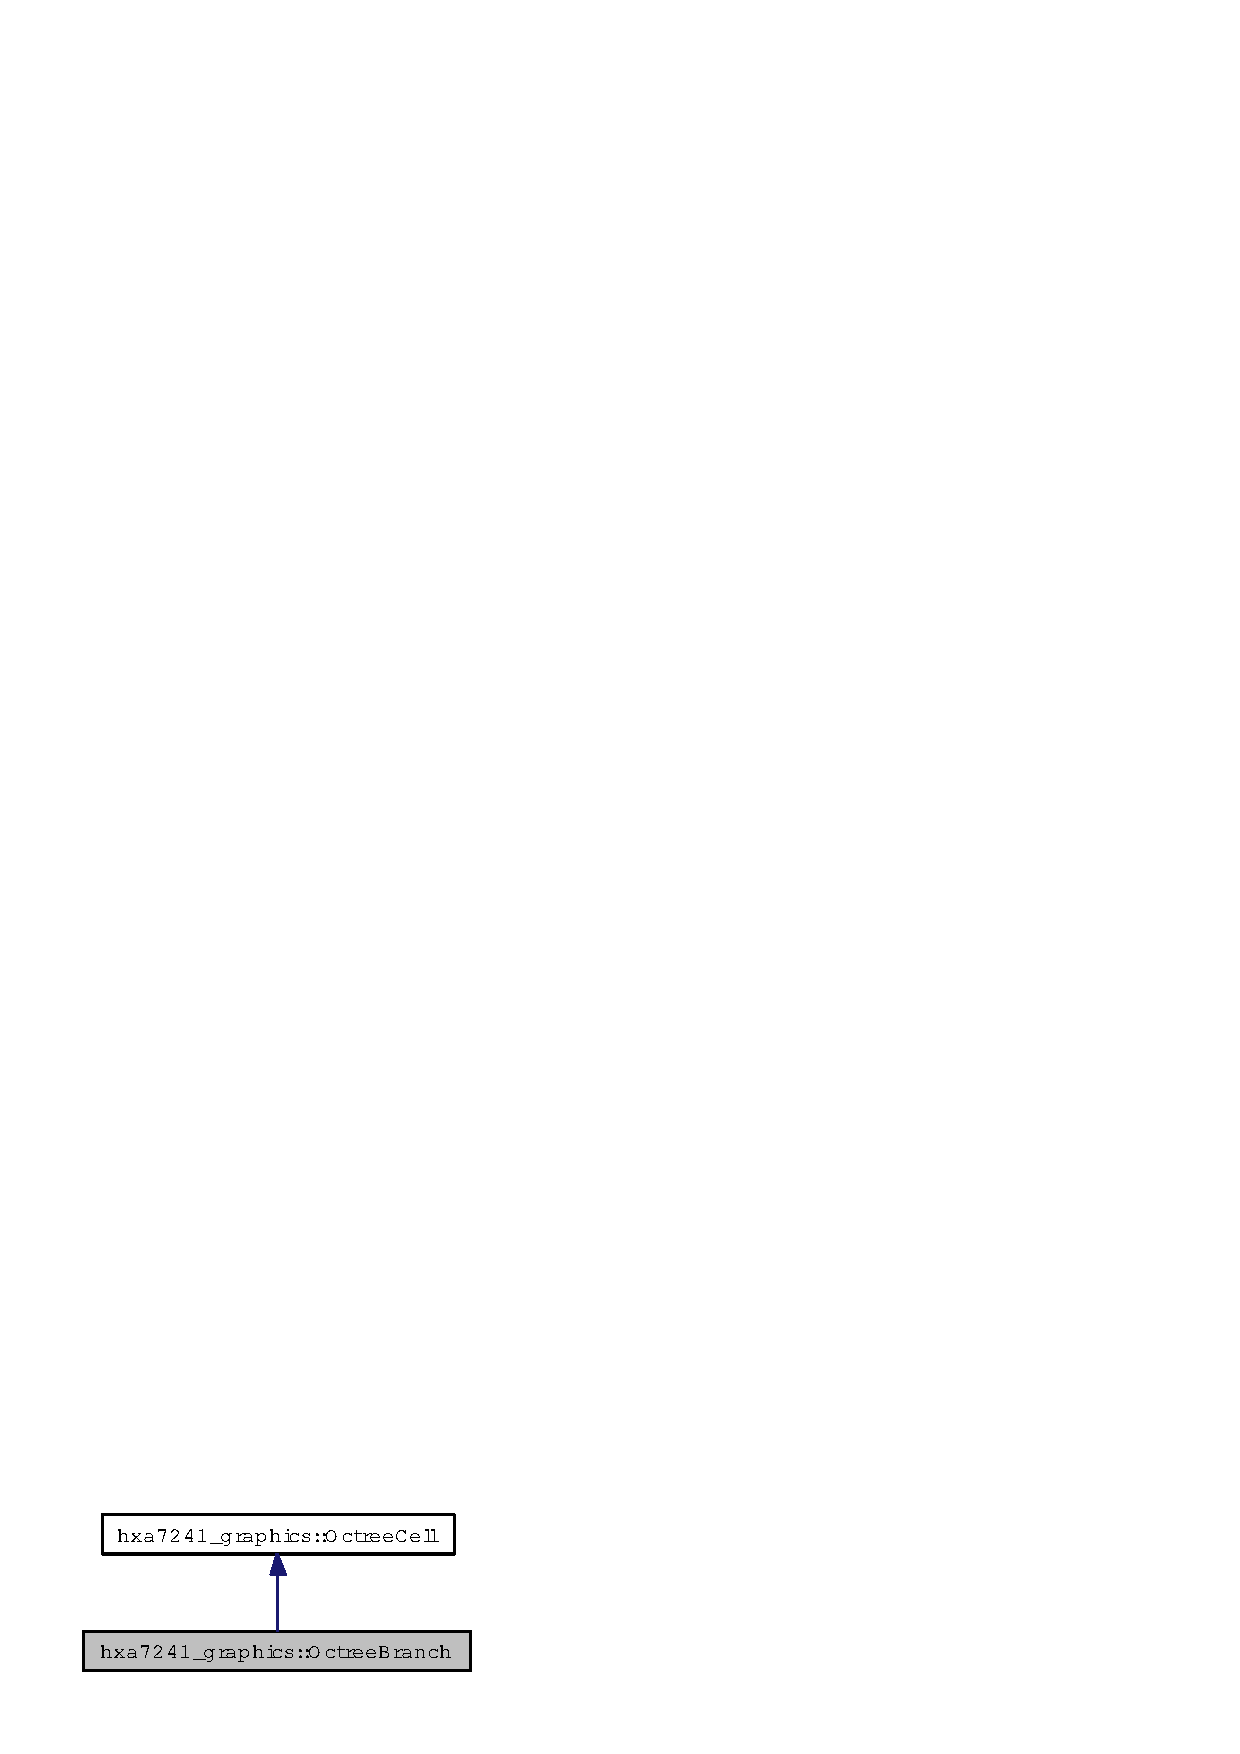
\includegraphics[width=115pt]{classhxa7241__graphics_1_1OctreeBranch__inherit__graph}
\end{center}
\end{figure}
Collaboration diagram for hxa7241\_\-graphics::Octree\-Branch:\begin{figure}[H]
\begin{center}
\leavevmode
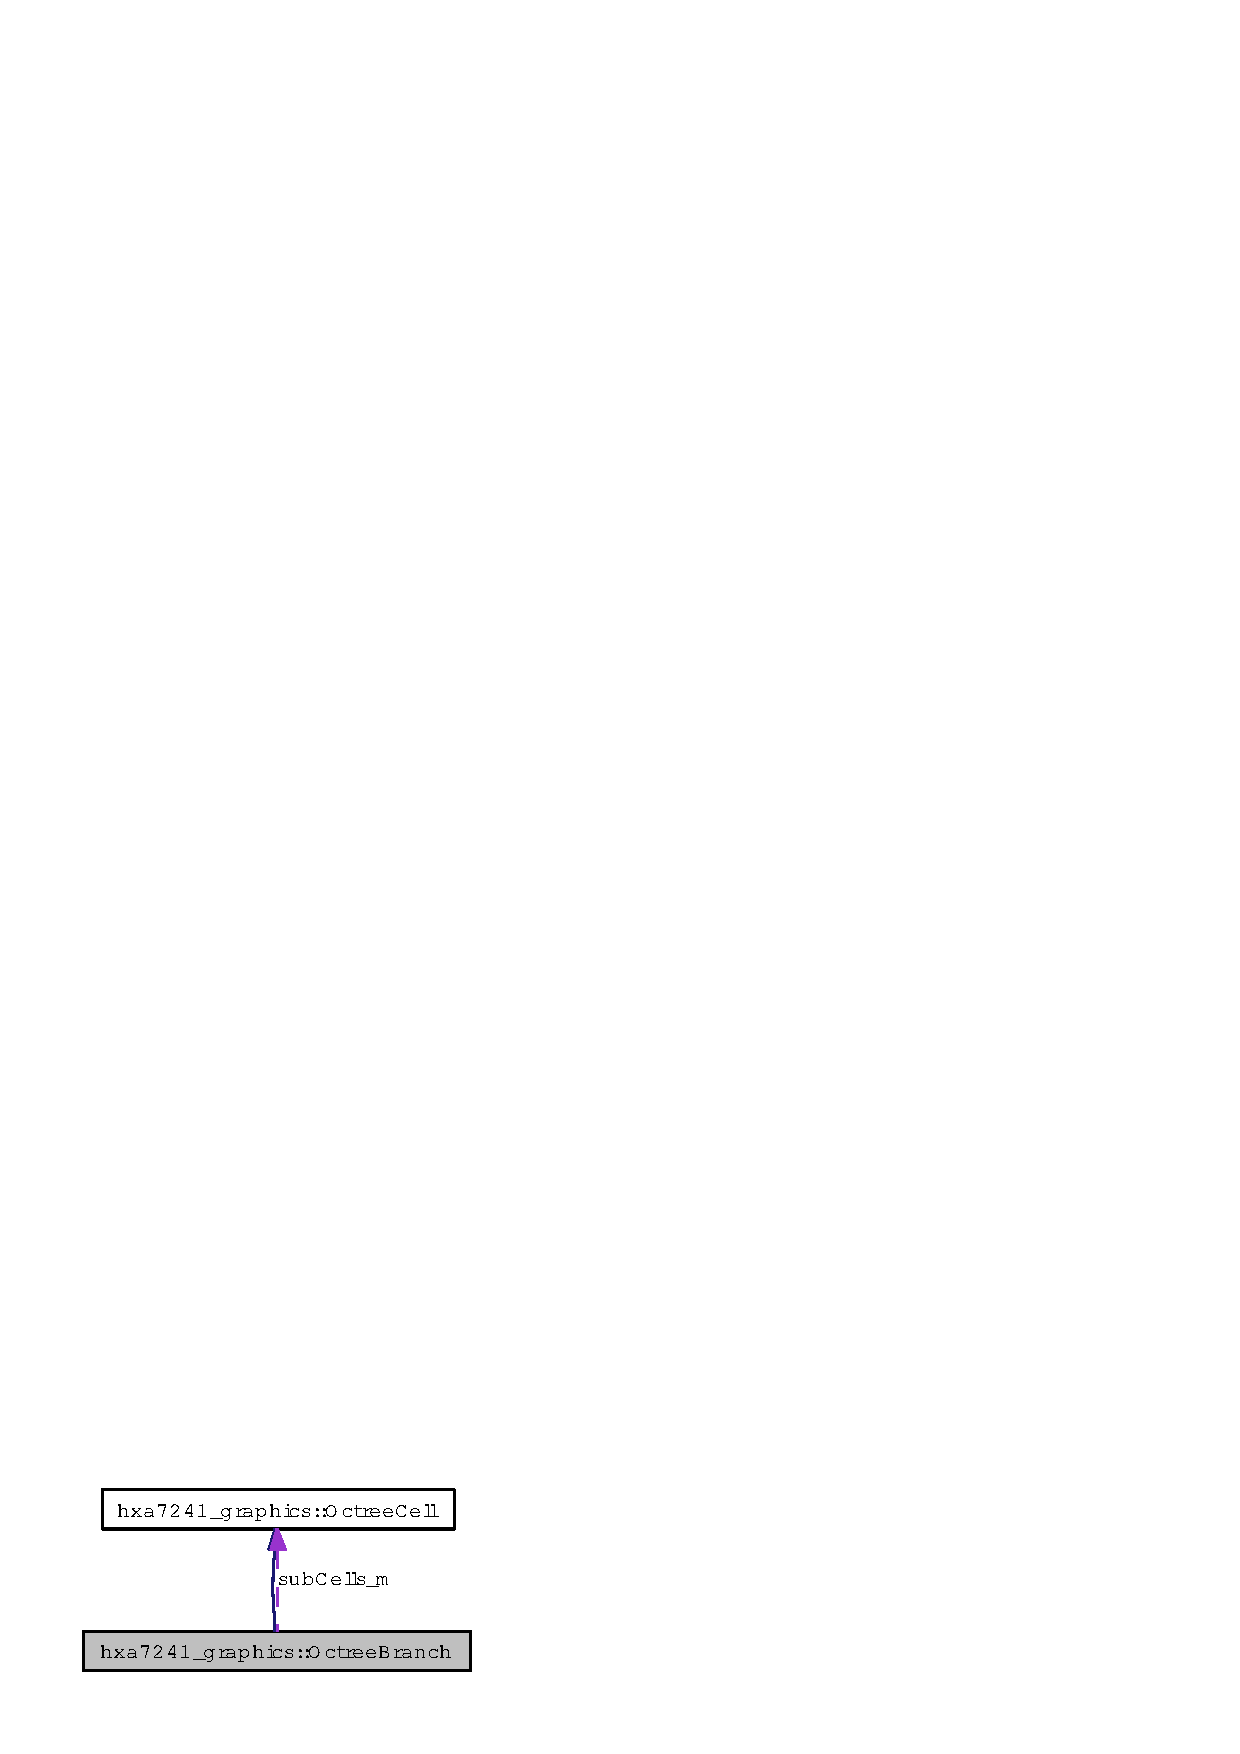
\includegraphics[width=115pt]{classhxa7241__graphics_1_1OctreeBranch__coll__graph}
\end{center}
\end{figure}
\subsection*{Public Member Functions}
\begin{CompactItemize}
\item 
{\bf Octree\-Branch} ()
\begin{CompactList}\small\item\em standard object services --------------------------------------------------- \item\end{CompactList}\item 
{\bf Octree\-Branch} (const {\bf Octree\-Data} \&this\-Data, const {\bf Array}$<$ const void $\ast$ $>$ \&items, const void $\ast$const p\-Item, const {\bf Octree\-Agent\-V} \&agent)
\item 
virtual {\bf $\sim$Octree\-Branch} ()
\item 
{\bf Octree\-Branch} (const {\bf Octree\-Branch} \&)
\item 
{\bf Octree\-Branch} \& {\bf operator=} (const {\bf Octree\-Branch} \&)
\item 
virtual void {\bf insert} (const {\bf Octree\-Data} \&this\-Data, {\bf Octree\-Cell} $\ast$\&p\-This, const void $\ast$p\-Item, const {\bf Octree\-Agent\-V} \&agent)
\begin{CompactList}\small\item\em commands ------------------------------------------------------------------- \item\end{CompactList}\item 
virtual bool {\bf remove} ({\bf Octree\-Cell} $\ast$\&p\-This, const void $\ast$p\-Item, const dword max\-Items\-Per\-Cell, dword \&item\-Count)
\item 
virtual void {\bf visit} (const {\bf Octree\-Data} \&this\-Data, {\bf Octree\-Visitor\-V} \&visitor) const
\begin{CompactList}\small\item\em queries -------------------------------------------------------------------- \item\end{CompactList}\item 
virtual {\bf Octree\-Cell} $\ast$ {\bf clone} () const
\item 
virtual void {\bf get\-Info} (dword \&byte\-Size, dword \&leaf\-Count, dword \&item\-Count, dword \&max\-Depth) const
\end{CompactItemize}
\subsection*{Static Public Member Functions}
\begin{CompactItemize}
\item 
static void {\bf continue\-Visit} (const {\bf Octree\-Cell} $\ast$sub\-Cells[8], const {\bf Octree\-Data} \&octree\-Data, dword sub\-Cell\-Index, {\bf Octree\-Visitor\-V} \&visitor)
\begin{CompactList}\small\item\em statics -------------------------------------------------------------------- \item\end{CompactList}\end{CompactItemize}
\subsection*{Protected Member Functions}
\begin{CompactItemize}
\item 
virtual void {\bf zero\-Sub\-Cells} ()
\begin{CompactList}\small\item\em implementation ------------------------------------------------------------- \item\end{CompactList}\end{CompactItemize}


\subsection{Detailed Description}
Inner node implementation of an octree cell.\par
\par


Stores pointers to eight (at most) child cells.

sub\-Cells\_\-m elements can be null, or point to an \doxyref{Octree\-Cell}{p.}{classhxa7241__graphics_1_1OctreeCell} instance. 



\subsection{Constructor \& Destructor Documentation}
\index{hxa7241_graphics::OctreeBranch@{hxa7241\_\-graphics::Octree\-Branch}!OctreeBranch@{OctreeBranch}}
\index{OctreeBranch@{OctreeBranch}!hxa7241_graphics::OctreeBranch@{hxa7241\_\-graphics::Octree\-Branch}}
\subsubsection{\setlength{\rightskip}{0pt plus 5cm}Octree\-Branch::Octree\-Branch ()}\label{classhxa7241__graphics_1_1OctreeBranch_42f7249c1578dfc66294655e783fe21e}


standard object services --------------------------------------------------- 

\index{hxa7241_graphics::OctreeBranch@{hxa7241\_\-graphics::Octree\-Branch}!OctreeBranch@{OctreeBranch}}
\index{OctreeBranch@{OctreeBranch}!hxa7241_graphics::OctreeBranch@{hxa7241\_\-graphics::Octree\-Branch}}
\subsubsection{\setlength{\rightskip}{0pt plus 5cm}Octree\-Branch::Octree\-Branch (const {\bf Octree\-Data} \& {\em this\-Data}, const {\bf Array}$<$ const void $\ast$ $>$ \& {\em items}, const void $\ast$const {\em p\-Item}, const {\bf Octree\-Agent\-V} \& {\em agent})}\label{classhxa7241__graphics_1_1OctreeBranch_77e0c99abc50b6d5fb1fb0687aa0608a}


\index{hxa7241_graphics::OctreeBranch@{hxa7241\_\-graphics::Octree\-Branch}!~OctreeBranch@{$\sim$OctreeBranch}}
\index{~OctreeBranch@{$\sim$OctreeBranch}!hxa7241_graphics::OctreeBranch@{hxa7241\_\-graphics::Octree\-Branch}}
\subsubsection{\setlength{\rightskip}{0pt plus 5cm}Octree\-Branch::$\sim$Octree\-Branch ()\hspace{0.3cm}{\tt  [virtual]}}\label{classhxa7241__graphics_1_1OctreeBranch_e2f09bec5e9597629c49f0290ead1e0e}


\index{hxa7241_graphics::OctreeBranch@{hxa7241\_\-graphics::Octree\-Branch}!OctreeBranch@{OctreeBranch}}
\index{OctreeBranch@{OctreeBranch}!hxa7241_graphics::OctreeBranch@{hxa7241\_\-graphics::Octree\-Branch}}
\subsubsection{\setlength{\rightskip}{0pt plus 5cm}Octree\-Branch::Octree\-Branch (const {\bf Octree\-Branch} \&)}\label{classhxa7241__graphics_1_1OctreeBranch_46906fb5f7b7000105fc38782392b418}




\subsection{Member Function Documentation}
\index{hxa7241_graphics::OctreeBranch@{hxa7241\_\-graphics::Octree\-Branch}!operator=@{operator=}}
\index{operator=@{operator=}!hxa7241_graphics::OctreeBranch@{hxa7241\_\-graphics::Octree\-Branch}}
\subsubsection{\setlength{\rightskip}{0pt plus 5cm}{\bf Octree\-Branch} \& Octree\-Branch::operator= (const {\bf Octree\-Branch} \&)}\label{classhxa7241__graphics_1_1OctreeBranch_1197934b2cd33dcb793a7f772f4355d7}


\index{hxa7241_graphics::OctreeBranch@{hxa7241\_\-graphics::Octree\-Branch}!insert@{insert}}
\index{insert@{insert}!hxa7241_graphics::OctreeBranch@{hxa7241\_\-graphics::Octree\-Branch}}
\subsubsection{\setlength{\rightskip}{0pt plus 5cm}void Octree\-Branch::insert (const {\bf Octree\-Data} \& {\em this\-Data}, {\bf Octree\-Cell} $\ast$\& {\em p\-This}, const void $\ast$ {\em p\-Item}, const {\bf Octree\-Agent\-V} \& {\em agent})\hspace{0.3cm}{\tt  [virtual]}}\label{classhxa7241__graphics_1_1OctreeBranch_149057db8e68438f5639088abe618007}


commands ------------------------------------------------------------------- 



Implements {\bf hxa7241\_\-graphics::Octree\-Cell} \doxyref{}{p.}{classhxa7241__graphics_1_1OctreeCell_0cf5936ffeaca906be184ac654cd8053}.\index{hxa7241_graphics::OctreeBranch@{hxa7241\_\-graphics::Octree\-Branch}!remove@{remove}}
\index{remove@{remove}!hxa7241_graphics::OctreeBranch@{hxa7241\_\-graphics::Octree\-Branch}}
\subsubsection{\setlength{\rightskip}{0pt plus 5cm}bool Octree\-Branch::remove ({\bf Octree\-Cell} $\ast$\& {\em p\-This}, const void $\ast$ {\em p\-Item}, const dword {\em max\-Items\-Per\-Cell}, dword \& {\em item\-Count})\hspace{0.3cm}{\tt  [virtual]}}\label{classhxa7241__graphics_1_1OctreeBranch_a9f402a456021e56b8c7e7e6e48c7863}




Implements {\bf hxa7241\_\-graphics::Octree\-Cell} \doxyref{}{p.}{classhxa7241__graphics_1_1OctreeCell_74c11f0b4d5ef93959253206c3816417}.\index{hxa7241_graphics::OctreeBranch@{hxa7241\_\-graphics::Octree\-Branch}!visit@{visit}}
\index{visit@{visit}!hxa7241_graphics::OctreeBranch@{hxa7241\_\-graphics::Octree\-Branch}}
\subsubsection{\setlength{\rightskip}{0pt plus 5cm}void Octree\-Branch::visit (const {\bf Octree\-Data} \& {\em this\-Data}, {\bf Octree\-Visitor\-V} \& {\em visitor}) const\hspace{0.3cm}{\tt  [virtual]}}\label{classhxa7241__graphics_1_1OctreeBranch_54e5ca483f3e52f1ccbbcfcd3c384493}


queries -------------------------------------------------------------------- 



Implements {\bf hxa7241\_\-graphics::Octree\-Cell} \doxyref{}{p.}{classhxa7241__graphics_1_1OctreeCell_e0998c3188914314451880d40ebd1c35}.\index{hxa7241_graphics::OctreeBranch@{hxa7241\_\-graphics::Octree\-Branch}!clone@{clone}}
\index{clone@{clone}!hxa7241_graphics::OctreeBranch@{hxa7241\_\-graphics::Octree\-Branch}}
\subsubsection{\setlength{\rightskip}{0pt plus 5cm}{\bf Octree\-Cell} $\ast$ Octree\-Branch::clone () const\hspace{0.3cm}{\tt  [virtual]}}\label{classhxa7241__graphics_1_1OctreeBranch_ab0e9bbd1749dffd6a398f92086bc868}




Implements {\bf hxa7241\_\-graphics::Octree\-Cell} \doxyref{}{p.}{classhxa7241__graphics_1_1OctreeCell_6f10b6cebce798d4a3e96b8822584774}.\index{hxa7241_graphics::OctreeBranch@{hxa7241\_\-graphics::Octree\-Branch}!getInfo@{getInfo}}
\index{getInfo@{getInfo}!hxa7241_graphics::OctreeBranch@{hxa7241\_\-graphics::Octree\-Branch}}
\subsubsection{\setlength{\rightskip}{0pt plus 5cm}void Octree\-Branch::get\-Info (dword \& {\em byte\-Size}, dword \& {\em leaf\-Count}, dword \& {\em item\-Count}, dword \& {\em max\-Depth}) const\hspace{0.3cm}{\tt  [virtual]}}\label{classhxa7241__graphics_1_1OctreeBranch_50cfc01d866acf532b900fbec17c99b2}




Implements {\bf hxa7241\_\-graphics::Octree\-Cell} \doxyref{}{p.}{classhxa7241__graphics_1_1OctreeCell_d8b69169addb924c9ec3bb6ae70a932f}.\index{hxa7241_graphics::OctreeBranch@{hxa7241\_\-graphics::Octree\-Branch}!continueVisit@{continueVisit}}
\index{continueVisit@{continueVisit}!hxa7241_graphics::OctreeBranch@{hxa7241\_\-graphics::Octree\-Branch}}
\subsubsection{\setlength{\rightskip}{0pt plus 5cm}void Octree\-Branch::continue\-Visit (const {\bf Octree\-Cell} $\ast$ {\em sub\-Cells}[8], const {\bf Octree\-Data} \& {\em octree\-Data}, dword {\em sub\-Cell\-Index}, {\bf Octree\-Visitor\-V} \& {\em visitor})\hspace{0.3cm}{\tt  [static]}}\label{classhxa7241__graphics_1_1OctreeBranch_13c4d758a1c9b38f166e916c87ba1469}


statics -------------------------------------------------------------------- 

\index{hxa7241_graphics::OctreeBranch@{hxa7241\_\-graphics::Octree\-Branch}!zeroSubCells@{zeroSubCells}}
\index{zeroSubCells@{zeroSubCells}!hxa7241_graphics::OctreeBranch@{hxa7241\_\-graphics::Octree\-Branch}}
\subsubsection{\setlength{\rightskip}{0pt plus 5cm}void Octree\-Branch::zero\-Sub\-Cells ()\hspace{0.3cm}{\tt  [protected, virtual]}}\label{classhxa7241__graphics_1_1OctreeBranch_68364176bd78a9ffda2545ffa174d24b}


implementation ------------------------------------------------------------- 



The documentation for this class was generated from the following files:\begin{CompactItemize}
\item 
{\bf Octree\-Implementation.h}\item 
{\bf Octree\-Implementation.cc}\end{CompactItemize}

\section{hxa7241\_\-graphics::Octree\-Cell Class Reference}
\label{classhxa7241__graphics_1_1OctreeCell}\index{hxa7241_graphics::OctreeCell@{hxa7241\_\-graphics::OctreeCell}}
{\tt \#include $<$Octree\-Implementation.h$>$}

Inheritance diagram for hxa7241\_\-graphics::Octree\-Cell:\begin{figure}[H]
\begin{center}
\leavevmode
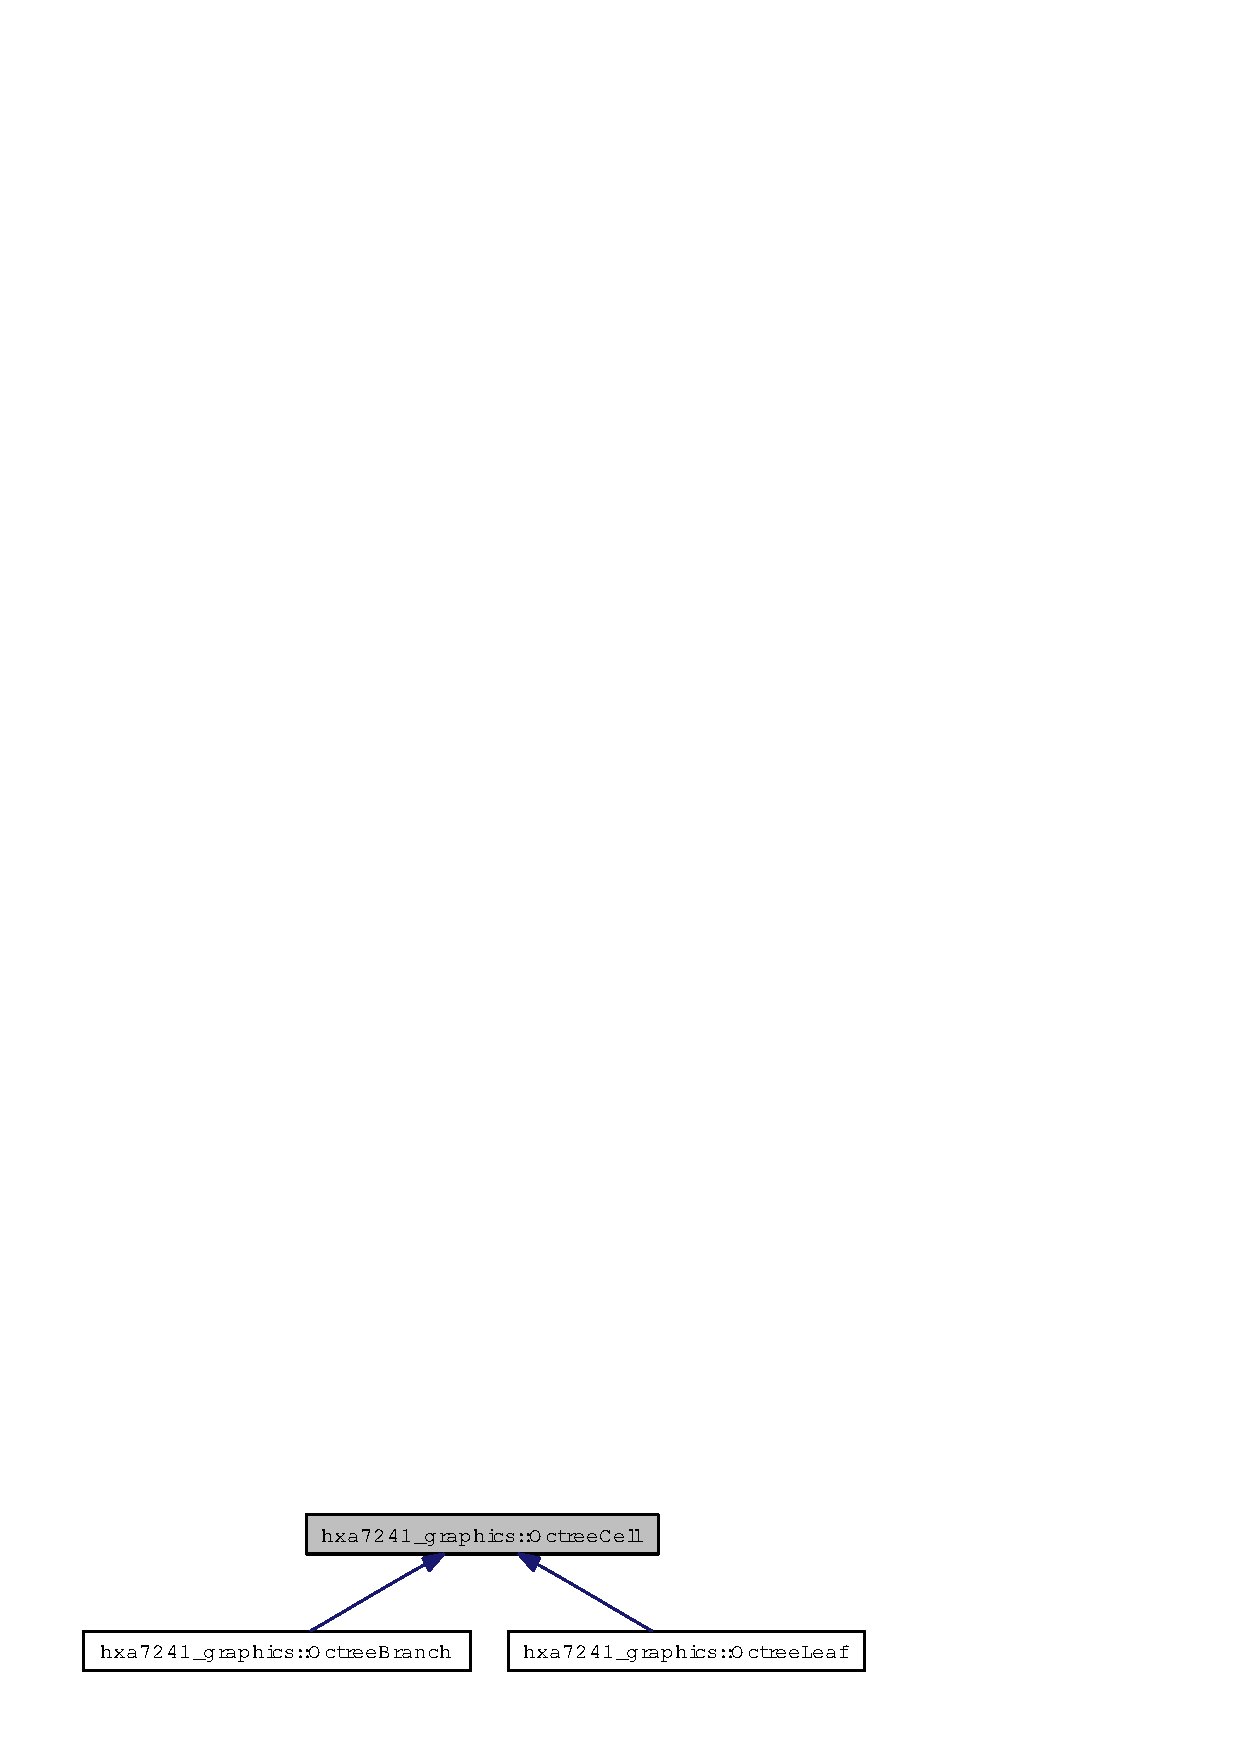
\includegraphics[width=209pt]{classhxa7241__graphics_1_1OctreeCell__inherit__graph}
\end{center}
\end{figure}
\subsection*{Public Member Functions}
\begin{CompactItemize}
\item 
virtual {\bf $\sim$Octree\-Cell} ()
\item 
virtual void {\bf insert} (const {\bf Octree\-Data} \&this\-Data, {\bf Octree\-Cell} $\ast$\&p\-This, const void $\ast$p\-Item, const {\bf Octree\-Agent\-V} \&agent)=0
\begin{CompactList}\small\item\em commands ------------------------------------------------------------------- \item\end{CompactList}\item 
virtual bool {\bf remove} ({\bf Octree\-Cell} $\ast$\&p\-This, const void $\ast$p\-Item, const dword max\-Items\-Per\-Cell, dword \&item\-Count)=0
\item 
virtual void {\bf visit} (const {\bf Octree\-Data} \&this\-Data, {\bf Octree\-Visitor\-V} \&visitor) const=0
\begin{CompactList}\small\item\em queries -------------------------------------------------------------------- \item\end{CompactList}\item 
virtual {\bf Octree\-Cell} $\ast$ {\bf clone} () const=0
\item 
virtual void {\bf get\-Info} (dword \&byte\-Size, dword \&leaf\-Count, dword \&item\-Count, dword \&max\-Depth) const=0
\end{CompactItemize}
\subsection*{Static Public Member Functions}
\begin{CompactItemize}
\item 
static {\bf Octree\-Cell} $\ast$ {\bf clone\-Non\-Zero} (const {\bf Octree\-Cell} $\ast$)
\begin{CompactList}\small\item\em statics -------------------------------------------------------------------- \item\end{CompactList}\end{CompactItemize}
\subsection*{Protected Member Functions}
\begin{CompactItemize}
\item 
{\bf Octree\-Cell} ()
\begin{CompactList}\small\item\em standard object services --------------------------------------------------- \item\end{CompactList}\end{CompactItemize}


\subsection{Detailed Description}
Abstract base for Composite types, for implementing \doxyref{Octree}{p.}{classhxa7241__graphics_1_1Octree} nodes.

Subcell numbering: \small\begin{alltt}
    y z       6 7
    |/   2 3  4 5
     -x  0 1
 \end{alltt}
\normalsize 
 in binary: \small\begin{alltt}
    y z           110 111
    |/   010 011  100 101
     -x  000 001
 \end{alltt}
\normalsize 
 



\subsection{Constructor \& Destructor Documentation}
\index{hxa7241_graphics::OctreeCell@{hxa7241\_\-graphics::Octree\-Cell}!OctreeCell@{OctreeCell}}
\index{OctreeCell@{OctreeCell}!hxa7241_graphics::OctreeCell@{hxa7241\_\-graphics::Octree\-Cell}}
\subsubsection{\setlength{\rightskip}{0pt plus 5cm}hxa7241\_\-graphics::Octree\-Cell::Octree\-Cell ()\hspace{0.3cm}{\tt  [inline, protected]}}\label{classhxa7241__graphics_1_1OctreeCell_3ec023c3d40078b33123c56dffe3444c}


standard object services --------------------------------------------------- 

\index{hxa7241_graphics::OctreeCell@{hxa7241\_\-graphics::Octree\-Cell}!~OctreeCell@{$\sim$OctreeCell}}
\index{~OctreeCell@{$\sim$OctreeCell}!hxa7241_graphics::OctreeCell@{hxa7241\_\-graphics::Octree\-Cell}}
\subsubsection{\setlength{\rightskip}{0pt plus 5cm}virtual hxa7241\_\-graphics::Octree\-Cell::$\sim$Octree\-Cell ()\hspace{0.3cm}{\tt  [inline, virtual]}}\label{classhxa7241__graphics_1_1OctreeCell_0a9f03261e22377df25fa908d000e514}




\subsection{Member Function Documentation}
\index{hxa7241_graphics::OctreeCell@{hxa7241\_\-graphics::Octree\-Cell}!insert@{insert}}
\index{insert@{insert}!hxa7241_graphics::OctreeCell@{hxa7241\_\-graphics::Octree\-Cell}}
\subsubsection{\setlength{\rightskip}{0pt plus 5cm}virtual void hxa7241\_\-graphics::Octree\-Cell::insert (const {\bf Octree\-Data} \& {\em this\-Data}, {\bf Octree\-Cell} $\ast$\& {\em p\-This}, const void $\ast$ {\em p\-Item}, const {\bf Octree\-Agent\-V} \& {\em agent})\hspace{0.3cm}{\tt  [pure virtual]}}\label{classhxa7241__graphics_1_1OctreeCell_0cf5936ffeaca906be184ac654cd8053}


commands ------------------------------------------------------------------- 



Implemented in {\bf hxa7241\_\-graphics::Octree\-Branch} \doxyref{}{p.}{classhxa7241__graphics_1_1OctreeBranch_149057db8e68438f5639088abe618007}, and {\bf hxa7241\_\-graphics::Octree\-Leaf} \doxyref{}{p.}{classhxa7241__graphics_1_1OctreeLeaf_7c6393f830a72b179948dd5bee97eeb4}.\index{hxa7241_graphics::OctreeCell@{hxa7241\_\-graphics::Octree\-Cell}!remove@{remove}}
\index{remove@{remove}!hxa7241_graphics::OctreeCell@{hxa7241\_\-graphics::Octree\-Cell}}
\subsubsection{\setlength{\rightskip}{0pt plus 5cm}virtual bool hxa7241\_\-graphics::Octree\-Cell::remove ({\bf Octree\-Cell} $\ast$\& {\em p\-This}, const void $\ast$ {\em p\-Item}, const dword {\em max\-Items\-Per\-Cell}, dword \& {\em item\-Count})\hspace{0.3cm}{\tt  [pure virtual]}}\label{classhxa7241__graphics_1_1OctreeCell_74c11f0b4d5ef93959253206c3816417}




Implemented in {\bf hxa7241\_\-graphics::Octree\-Branch} \doxyref{}{p.}{classhxa7241__graphics_1_1OctreeBranch_a9f402a456021e56b8c7e7e6e48c7863}, and {\bf hxa7241\_\-graphics::Octree\-Leaf} \doxyref{}{p.}{classhxa7241__graphics_1_1OctreeLeaf_64a170120344343a7f5309248aba2ab7}.\index{hxa7241_graphics::OctreeCell@{hxa7241\_\-graphics::Octree\-Cell}!visit@{visit}}
\index{visit@{visit}!hxa7241_graphics::OctreeCell@{hxa7241\_\-graphics::Octree\-Cell}}
\subsubsection{\setlength{\rightskip}{0pt plus 5cm}virtual void hxa7241\_\-graphics::Octree\-Cell::visit (const {\bf Octree\-Data} \& {\em this\-Data}, {\bf Octree\-Visitor\-V} \& {\em visitor}) const\hspace{0.3cm}{\tt  [pure virtual]}}\label{classhxa7241__graphics_1_1OctreeCell_e0998c3188914314451880d40ebd1c35}


queries -------------------------------------------------------------------- 



Implemented in {\bf hxa7241\_\-graphics::Octree\-Branch} \doxyref{}{p.}{classhxa7241__graphics_1_1OctreeBranch_54e5ca483f3e52f1ccbbcfcd3c384493}, and {\bf hxa7241\_\-graphics::Octree\-Leaf} \doxyref{}{p.}{classhxa7241__graphics_1_1OctreeLeaf_4dc0120fbd3d27f6628a507faf13d323}.\index{hxa7241_graphics::OctreeCell@{hxa7241\_\-graphics::Octree\-Cell}!clone@{clone}}
\index{clone@{clone}!hxa7241_graphics::OctreeCell@{hxa7241\_\-graphics::Octree\-Cell}}
\subsubsection{\setlength{\rightskip}{0pt plus 5cm}virtual {\bf Octree\-Cell}$\ast$ hxa7241\_\-graphics::Octree\-Cell::clone () const\hspace{0.3cm}{\tt  [pure virtual]}}\label{classhxa7241__graphics_1_1OctreeCell_6f10b6cebce798d4a3e96b8822584774}




Implemented in {\bf hxa7241\_\-graphics::Octree\-Branch} \doxyref{}{p.}{classhxa7241__graphics_1_1OctreeBranch_ab0e9bbd1749dffd6a398f92086bc868}, and {\bf hxa7241\_\-graphics::Octree\-Leaf} \doxyref{}{p.}{classhxa7241__graphics_1_1OctreeLeaf_0908765dbe95af75036abc65380a3aa8}.\index{hxa7241_graphics::OctreeCell@{hxa7241\_\-graphics::Octree\-Cell}!getInfo@{getInfo}}
\index{getInfo@{getInfo}!hxa7241_graphics::OctreeCell@{hxa7241\_\-graphics::Octree\-Cell}}
\subsubsection{\setlength{\rightskip}{0pt plus 5cm}virtual void hxa7241\_\-graphics::Octree\-Cell::get\-Info (dword \& {\em byte\-Size}, dword \& {\em leaf\-Count}, dword \& {\em item\-Count}, dword \& {\em max\-Depth}) const\hspace{0.3cm}{\tt  [pure virtual]}}\label{classhxa7241__graphics_1_1OctreeCell_d8b69169addb924c9ec3bb6ae70a932f}




Implemented in {\bf hxa7241\_\-graphics::Octree\-Branch} \doxyref{}{p.}{classhxa7241__graphics_1_1OctreeBranch_50cfc01d866acf532b900fbec17c99b2}, and {\bf hxa7241\_\-graphics::Octree\-Leaf} \doxyref{}{p.}{classhxa7241__graphics_1_1OctreeLeaf_ff8e9556edcae39b2d4fbd2db1d37b4f}.\index{hxa7241_graphics::OctreeCell@{hxa7241\_\-graphics::Octree\-Cell}!cloneNonZero@{cloneNonZero}}
\index{cloneNonZero@{cloneNonZero}!hxa7241_graphics::OctreeCell@{hxa7241\_\-graphics::Octree\-Cell}}
\subsubsection{\setlength{\rightskip}{0pt plus 5cm}{\bf Octree\-Cell} $\ast$ Octree\-Cell::clone\-Non\-Zero (const {\bf Octree\-Cell} $\ast$)\hspace{0.3cm}{\tt  [static]}}\label{classhxa7241__graphics_1_1OctreeCell_9f76513f2785740d5b786f44d12908e1}


statics -------------------------------------------------------------------- 



The documentation for this class was generated from the following files:\begin{CompactItemize}
\item 
{\bf Octree\-Implementation.h}\item 
{\bf Octree\-Implementation.cc}\end{CompactItemize}

\section{hxa7241\_\-graphics::Octree\-Data Class Reference}
\label{classhxa7241__graphics_1_1OctreeData}\index{hxa7241_graphics::OctreeData@{hxa7241\_\-graphics::OctreeData}}
{\tt \#include $<$Octree\-Auxiliary.h$>$}

Collaboration diagram for hxa7241\_\-graphics::Octree\-Data:\begin{figure}[H]
\begin{center}
\leavevmode
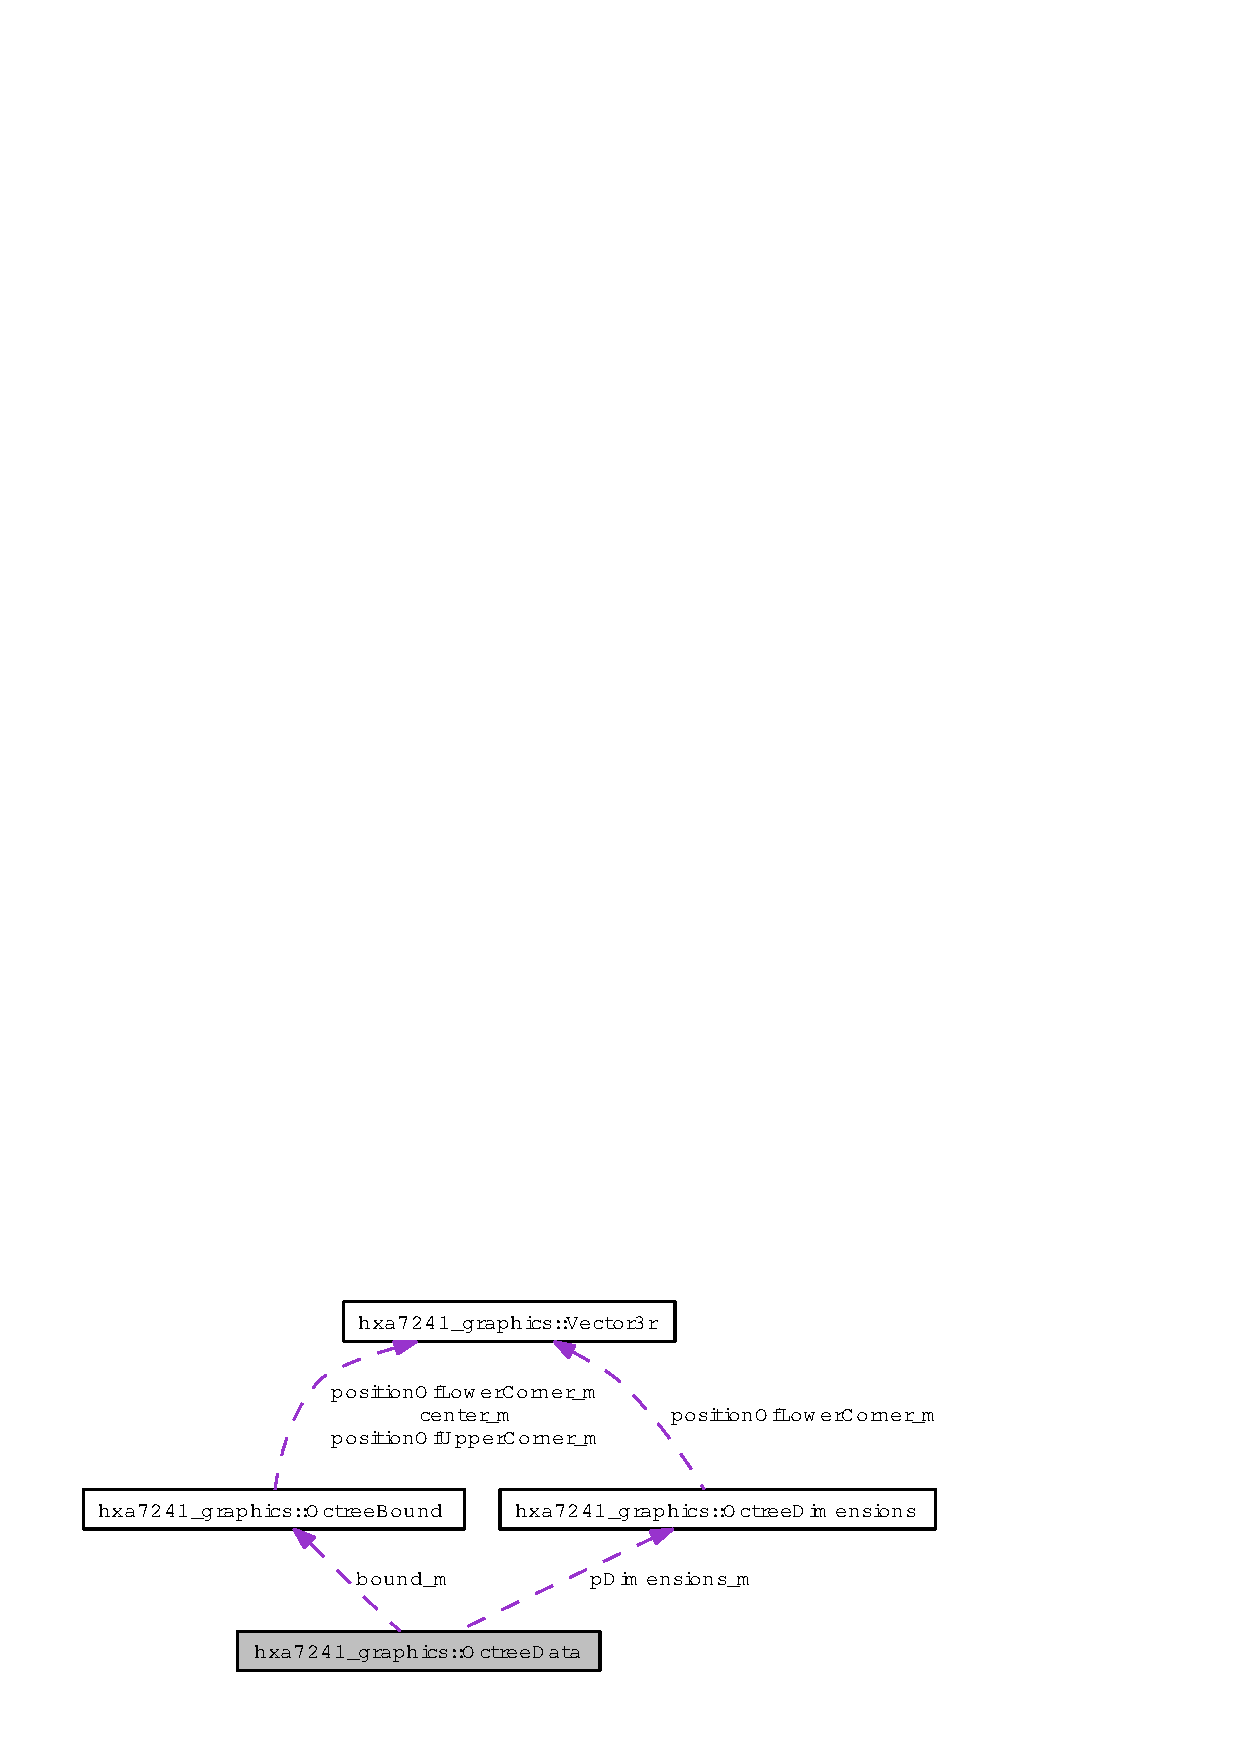
\includegraphics[width=232pt]{classhxa7241__graphics_1_1OctreeData__coll__graph}
\end{center}
\end{figure}
\subsection*{Public Member Functions}
\begin{CompactItemize}
\item 
{\bf Octree\-Data} (const {\bf Octree\-Dimensions} \&dimensions)
\begin{CompactList}\small\item\em standard object services --------------------------------------------------- \item\end{CompactList}\item 
{\bf Octree\-Data} (const {\bf Octree\-Data} \&parent\-Cell\-Data, dword sub\-Cell\-Index)
\item 
{\bf Octree\-Data} (const {\bf Octree\-Data} \&, const {\bf Octree\-Dimensions} \&)
\item 
{\bf $\sim$Octree\-Data} ()
\item 
{\bf Octree\-Data} (const {\bf Octree\-Data} \&)
\item 
{\bf Octree\-Data} \& {\bf operator=} (const {\bf Octree\-Data} \&)
\item 
const {\bf Octree\-Bound} \& {\bf get\-Bound} () const
\begin{CompactList}\small\item\em \doxyref{Octree\-Data}{p.}{classhxa7241__graphics_1_1OctreeData} -----------------------------------------------------------------. \item\end{CompactList}\item 
dword {\bf get\-Level} () const
\item 
const {\bf Octree\-Dimensions} \& {\bf get\-Dimensions} () const
\item 
bool {\bf is\-Subdivide} (dword item\-Count) const
\end{CompactItemize}


\subsection{Detailed Description}
\doxyref{Octree}{p.}{classhxa7241__graphics_1_1Octree} cell data during traversal.\par
\par


Constant.\par
\par


To be made during each level of tree descent, so storage is avoided, except to hold one at the root.\par
\par


Subcell numbering: \small\begin{alltt}
    y z       6 7
    |/   2 3  4 5
     -x  0 1
 \end{alltt}
\normalsize 
 in binary: \small\begin{alltt}
    y z           110 111
    |/   010 011  100 101
     -x  000 001
 \end{alltt}
\normalsize 


\begin{Desc}
\item[See also:]\doxyref{Octree\-Bound}{p.}{classhxa7241__graphics_1_1OctreeBound} 

\doxyref{Octree\-Dimensions}{p.}{classhxa7241__graphics_1_1OctreeDimensions} \end{Desc}




\subsection{Constructor \& Destructor Documentation}
\index{hxa7241_graphics::OctreeData@{hxa7241\_\-graphics::Octree\-Data}!OctreeData@{OctreeData}}
\index{OctreeData@{OctreeData}!hxa7241_graphics::OctreeData@{hxa7241\_\-graphics::Octree\-Data}}
\subsubsection{\setlength{\rightskip}{0pt plus 5cm}Octree\-Data::Octree\-Data (const {\bf Octree\-Dimensions} \& {\em dimensions})\hspace{0.3cm}{\tt  [explicit]}}\label{classhxa7241__graphics_1_1OctreeData_54da8bd41940df4ff7a142b31478b430}


standard object services --------------------------------------------------- 

\index{hxa7241_graphics::OctreeData@{hxa7241\_\-graphics::Octree\-Data}!OctreeData@{OctreeData}}
\index{OctreeData@{OctreeData}!hxa7241_graphics::OctreeData@{hxa7241\_\-graphics::Octree\-Data}}
\subsubsection{\setlength{\rightskip}{0pt plus 5cm}Octree\-Data::Octree\-Data (const {\bf Octree\-Data} \& {\em parent\-Cell\-Data}, dword {\em sub\-Cell\-Index})}\label{classhxa7241__graphics_1_1OctreeData_0d603f5bdf89d8d3b20063bc4dafad76}


\index{hxa7241_graphics::OctreeData@{hxa7241\_\-graphics::Octree\-Data}!OctreeData@{OctreeData}}
\index{OctreeData@{OctreeData}!hxa7241_graphics::OctreeData@{hxa7241\_\-graphics::Octree\-Data}}
\subsubsection{\setlength{\rightskip}{0pt plus 5cm}Octree\-Data::Octree\-Data (const {\bf Octree\-Data} \&, const {\bf Octree\-Dimensions} \&)}\label{classhxa7241__graphics_1_1OctreeData_20f196fe3a6b69c4dd9a548d496a1bb5}


\index{hxa7241_graphics::OctreeData@{hxa7241\_\-graphics::Octree\-Data}!~OctreeData@{$\sim$OctreeData}}
\index{~OctreeData@{$\sim$OctreeData}!hxa7241_graphics::OctreeData@{hxa7241\_\-graphics::Octree\-Data}}
\subsubsection{\setlength{\rightskip}{0pt plus 5cm}Octree\-Data::$\sim$Octree\-Data ()}\label{classhxa7241__graphics_1_1OctreeData_ae27d150cbba477c768d0adcb238b407}


\index{hxa7241_graphics::OctreeData@{hxa7241\_\-graphics::Octree\-Data}!OctreeData@{OctreeData}}
\index{OctreeData@{OctreeData}!hxa7241_graphics::OctreeData@{hxa7241\_\-graphics::Octree\-Data}}
\subsubsection{\setlength{\rightskip}{0pt plus 5cm}Octree\-Data::Octree\-Data (const {\bf Octree\-Data} \&)}\label{classhxa7241__graphics_1_1OctreeData_9ccce80b11b4097e4df6f194deccacd2}




\subsection{Member Function Documentation}
\index{hxa7241_graphics::OctreeData@{hxa7241\_\-graphics::Octree\-Data}!operator=@{operator=}}
\index{operator=@{operator=}!hxa7241_graphics::OctreeData@{hxa7241\_\-graphics::Octree\-Data}}
\subsubsection{\setlength{\rightskip}{0pt plus 5cm}{\bf Octree\-Data} \& Octree\-Data::operator= (const {\bf Octree\-Data} \&)}\label{classhxa7241__graphics_1_1OctreeData_a5534836a9935194d9e835aac9819e70}


\index{hxa7241_graphics::OctreeData@{hxa7241\_\-graphics::Octree\-Data}!getBound@{getBound}}
\index{getBound@{getBound}!hxa7241_graphics::OctreeData@{hxa7241\_\-graphics::Octree\-Data}}
\subsubsection{\setlength{\rightskip}{0pt plus 5cm}const {\bf Octree\-Bound} \& hxa7241\_\-graphics::Octree\-Data::get\-Bound () const\hspace{0.3cm}{\tt  [inline]}}\label{classhxa7241__graphics_1_1OctreeData_701d81e5a8998ec5ea612c7248380e73}


\doxyref{Octree\-Data}{p.}{classhxa7241__graphics_1_1OctreeData} -----------------------------------------------------------------. 

\index{hxa7241_graphics::OctreeData@{hxa7241\_\-graphics::Octree\-Data}!getLevel@{getLevel}}
\index{getLevel@{getLevel}!hxa7241_graphics::OctreeData@{hxa7241\_\-graphics::Octree\-Data}}
\subsubsection{\setlength{\rightskip}{0pt plus 5cm}dword hxa7241\_\-graphics::Octree\-Data::get\-Level () const\hspace{0.3cm}{\tt  [inline]}}\label{classhxa7241__graphics_1_1OctreeData_9217bee4b6c887e326b243f1fe851462}


\index{hxa7241_graphics::OctreeData@{hxa7241\_\-graphics::Octree\-Data}!getDimensions@{getDimensions}}
\index{getDimensions@{getDimensions}!hxa7241_graphics::OctreeData@{hxa7241\_\-graphics::Octree\-Data}}
\subsubsection{\setlength{\rightskip}{0pt plus 5cm}const {\bf Octree\-Dimensions} \& hxa7241\_\-graphics::Octree\-Data::get\-Dimensions () const\hspace{0.3cm}{\tt  [inline]}}\label{classhxa7241__graphics_1_1OctreeData_deeb7c14a69fc59bcea61cf1bd4bd99e}


\index{hxa7241_graphics::OctreeData@{hxa7241\_\-graphics::Octree\-Data}!isSubdivide@{isSubdivide}}
\index{isSubdivide@{isSubdivide}!hxa7241_graphics::OctreeData@{hxa7241\_\-graphics::Octree\-Data}}
\subsubsection{\setlength{\rightskip}{0pt plus 5cm}bool hxa7241\_\-graphics::Octree\-Data::is\-Subdivide (dword {\em item\-Count}) const\hspace{0.3cm}{\tt  [inline]}}\label{classhxa7241__graphics_1_1OctreeData_37d26c210294d5c56b30b6588d7822a9}




The documentation for this class was generated from the following files:\begin{CompactItemize}
\item 
{\bf Octree\-Auxiliary.h}\item 
{\bf Octree\-Auxiliary.cc}\end{CompactItemize}

\section{hxa7241\_\-graphics::Octree\-Dimensions Class Reference}
\label{classhxa7241__graphics_1_1OctreeDimensions}\index{hxa7241_graphics::OctreeDimensions@{hxa7241\_\-graphics::OctreeDimensions}}
{\tt \#include $<$Octree\-Auxiliary.h$>$}

Collaboration diagram for hxa7241\_\-graphics::Octree\-Dimensions:\begin{figure}[H]
\begin{center}
\leavevmode
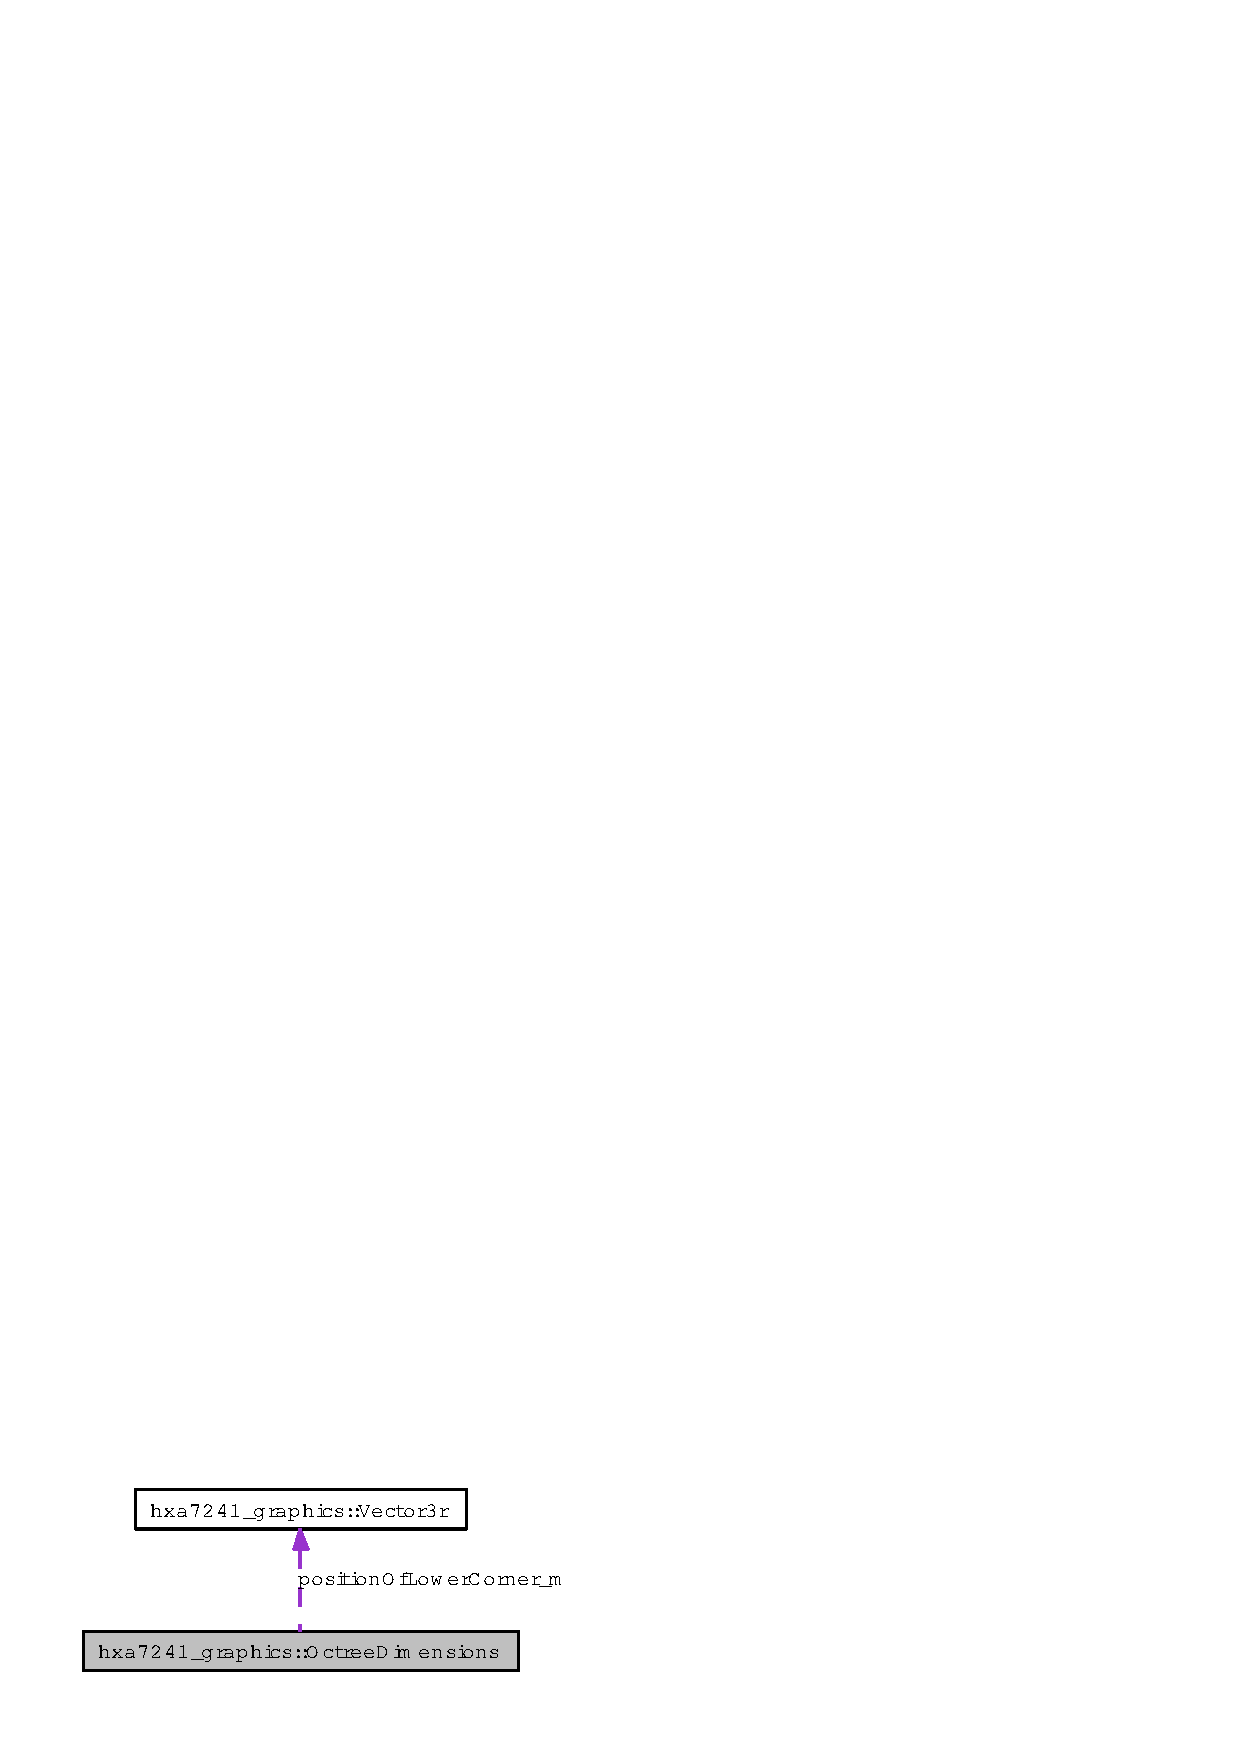
\includegraphics[width=139pt]{classhxa7241__graphics_1_1OctreeDimensions__coll__graph}
\end{center}
\end{figure}
\subsection*{Public Member Functions}
\begin{CompactItemize}
\item 
{\bf Octree\-Dimensions} (const {\bf Vector3r} \&position\-Of\-Lower\-Corner, real size, dword max\-Item\-Count\-Per\-Cell, dword max\-Level\-Count, real min\-Cell\-Size)
\begin{CompactList}\small\item\em standard object services --------------------------------------------------- \item\end{CompactList}\item 
{\bf $\sim$Octree\-Dimensions} ()
\item 
{\bf Octree\-Dimensions} (const {\bf Octree\-Dimensions} \&)
\item 
{\bf Octree\-Dimensions} \& {\bf operator=} (const {\bf Octree\-Dimensions} \&)
\item 
const {\bf Vector3r} \& {\bf get\-Position} () const
\begin{CompactList}\small\item\em \doxyref{Octree\-Dimensions}{p.}{classhxa7241__graphics_1_1OctreeDimensions} -----------------------------------------------------------. \item\end{CompactList}\item 
real {\bf get\-Size} () const
\item 
dword {\bf get\-Max\-Item\-Count\-Per\-Cell} () const
\item 
dword {\bf get\-Max\-Level\-Count} () const
\item 
real {\bf get\-Min\-Cell\-Size} () const
\item 
bool {\bf is\-Subdivide} (dword item\-Count, dword level, real size) const
\begin{CompactList}\small\item\em queries -------------------------------------------------------------------- \item\end{CompactList}\end{CompactItemize}


\subsection{Detailed Description}
Global octree data -- one instance for whole octree.\par
\par


Constant.

size\_\-m $>$= 0\par
 max\-Items\-Per\-Cell\_\-m $>$= 1\par
 max\-Level\_\-m $>$= 0 and $<$= MAX\_\-LEVEL\par
 min\-Size\_\-m $>$= MIN\_\-SIZE and $<$= size\_\-m\par
 



\subsection{Constructor \& Destructor Documentation}
\index{hxa7241_graphics::OctreeDimensions@{hxa7241\_\-graphics::Octree\-Dimensions}!OctreeDimensions@{OctreeDimensions}}
\index{OctreeDimensions@{OctreeDimensions}!hxa7241_graphics::OctreeDimensions@{hxa7241\_\-graphics::Octree\-Dimensions}}
\subsubsection{\setlength{\rightskip}{0pt plus 5cm}Octree\-Dimensions::Octree\-Dimensions (const {\bf Vector3r} \& {\em position\-Of\-Lower\-Corner}, real {\em size}, dword {\em max\-Item\-Count\-Per\-Cell}, dword {\em max\-Level\-Count}, real {\em min\-Cell\-Size})}\label{classhxa7241__graphics_1_1OctreeDimensions_8833b81e598e0b1cc7b98daee31288ee}


standard object services --------------------------------------------------- 

\index{hxa7241_graphics::OctreeDimensions@{hxa7241\_\-graphics::Octree\-Dimensions}!~OctreeDimensions@{$\sim$OctreeDimensions}}
\index{~OctreeDimensions@{$\sim$OctreeDimensions}!hxa7241_graphics::OctreeDimensions@{hxa7241\_\-graphics::Octree\-Dimensions}}
\subsubsection{\setlength{\rightskip}{0pt plus 5cm}Octree\-Dimensions::$\sim$Octree\-Dimensions ()}\label{classhxa7241__graphics_1_1OctreeDimensions_ffbe2fcaf3db49be65431d6c01060615}


\index{hxa7241_graphics::OctreeDimensions@{hxa7241\_\-graphics::Octree\-Dimensions}!OctreeDimensions@{OctreeDimensions}}
\index{OctreeDimensions@{OctreeDimensions}!hxa7241_graphics::OctreeDimensions@{hxa7241\_\-graphics::Octree\-Dimensions}}
\subsubsection{\setlength{\rightskip}{0pt plus 5cm}Octree\-Dimensions::Octree\-Dimensions (const {\bf Octree\-Dimensions} \&)}\label{classhxa7241__graphics_1_1OctreeDimensions_4199b3e8021c23a27d9a9a6cf820c90f}




\subsection{Member Function Documentation}
\index{hxa7241_graphics::OctreeDimensions@{hxa7241\_\-graphics::Octree\-Dimensions}!operator=@{operator=}}
\index{operator=@{operator=}!hxa7241_graphics::OctreeDimensions@{hxa7241\_\-graphics::Octree\-Dimensions}}
\subsubsection{\setlength{\rightskip}{0pt plus 5cm}{\bf Octree\-Dimensions} \& Octree\-Dimensions::operator= (const {\bf Octree\-Dimensions} \&)}\label{classhxa7241__graphics_1_1OctreeDimensions_bc30f675fd6ea1af90dbac8b35aa8e76}


\index{hxa7241_graphics::OctreeDimensions@{hxa7241\_\-graphics::Octree\-Dimensions}!getPosition@{getPosition}}
\index{getPosition@{getPosition}!hxa7241_graphics::OctreeDimensions@{hxa7241\_\-graphics::Octree\-Dimensions}}
\subsubsection{\setlength{\rightskip}{0pt plus 5cm}const {\bf Vector3r} \& hxa7241\_\-graphics::Octree\-Dimensions::get\-Position () const\hspace{0.3cm}{\tt  [inline]}}\label{classhxa7241__graphics_1_1OctreeDimensions_4c7bd5dd4adc2dac72c9436576400f7b}


\doxyref{Octree\-Dimensions}{p.}{classhxa7241__graphics_1_1OctreeDimensions} -----------------------------------------------------------. 

\index{hxa7241_graphics::OctreeDimensions@{hxa7241\_\-graphics::Octree\-Dimensions}!getSize@{getSize}}
\index{getSize@{getSize}!hxa7241_graphics::OctreeDimensions@{hxa7241\_\-graphics::Octree\-Dimensions}}
\subsubsection{\setlength{\rightskip}{0pt plus 5cm}real hxa7241\_\-graphics::Octree\-Dimensions::get\-Size () const\hspace{0.3cm}{\tt  [inline]}}\label{classhxa7241__graphics_1_1OctreeDimensions_e8157dd7145cdfc09053c0764be008bd}


\index{hxa7241_graphics::OctreeDimensions@{hxa7241\_\-graphics::Octree\-Dimensions}!getMaxItemCountPerCell@{getMaxItemCountPerCell}}
\index{getMaxItemCountPerCell@{getMaxItemCountPerCell}!hxa7241_graphics::OctreeDimensions@{hxa7241\_\-graphics::Octree\-Dimensions}}
\subsubsection{\setlength{\rightskip}{0pt plus 5cm}dword hxa7241\_\-graphics::Octree\-Dimensions::get\-Max\-Item\-Count\-Per\-Cell () const\hspace{0.3cm}{\tt  [inline]}}\label{classhxa7241__graphics_1_1OctreeDimensions_0ed4f1e98ce964e4db1b962d6081a95c}


\index{hxa7241_graphics::OctreeDimensions@{hxa7241\_\-graphics::Octree\-Dimensions}!getMaxLevelCount@{getMaxLevelCount}}
\index{getMaxLevelCount@{getMaxLevelCount}!hxa7241_graphics::OctreeDimensions@{hxa7241\_\-graphics::Octree\-Dimensions}}
\subsubsection{\setlength{\rightskip}{0pt plus 5cm}dword hxa7241\_\-graphics::Octree\-Dimensions::get\-Max\-Level\-Count () const\hspace{0.3cm}{\tt  [inline]}}\label{classhxa7241__graphics_1_1OctreeDimensions_566756ecf78d3ec6108fc46931cb4673}


\index{hxa7241_graphics::OctreeDimensions@{hxa7241\_\-graphics::Octree\-Dimensions}!getMinCellSize@{getMinCellSize}}
\index{getMinCellSize@{getMinCellSize}!hxa7241_graphics::OctreeDimensions@{hxa7241\_\-graphics::Octree\-Dimensions}}
\subsubsection{\setlength{\rightskip}{0pt plus 5cm}real hxa7241\_\-graphics::Octree\-Dimensions::get\-Min\-Cell\-Size () const\hspace{0.3cm}{\tt  [inline]}}\label{classhxa7241__graphics_1_1OctreeDimensions_16b54be6af6e83883c70d9a6931ecbd3}


\index{hxa7241_graphics::OctreeDimensions@{hxa7241\_\-graphics::Octree\-Dimensions}!isSubdivide@{isSubdivide}}
\index{isSubdivide@{isSubdivide}!hxa7241_graphics::OctreeDimensions@{hxa7241\_\-graphics::Octree\-Dimensions}}
\subsubsection{\setlength{\rightskip}{0pt plus 5cm}bool Octree\-Dimensions::is\-Subdivide (dword {\em item\-Count}, dword {\em level}, real {\em size}) const}\label{classhxa7241__graphics_1_1OctreeDimensions_eb7d8289a3348734e224bc6c2f075e97}


queries -------------------------------------------------------------------- 



The documentation for this class was generated from the following files:\begin{CompactItemize}
\item 
{\bf Octree\-Auxiliary.h}\item 
{\bf Octree\-Auxiliary.cc}\end{CompactItemize}

\section{hxa7241\_\-graphics::Octree\-Leaf Class Reference}
\label{classhxa7241__graphics_1_1OctreeLeaf}\index{hxa7241_graphics::OctreeLeaf@{hxa7241\_\-graphics::OctreeLeaf}}
{\tt \#include $<$Octree\-Implementation.h$>$}

Inheritance diagram for hxa7241\_\-graphics::Octree\-Leaf:\begin{figure}[H]
\begin{center}
\leavevmode
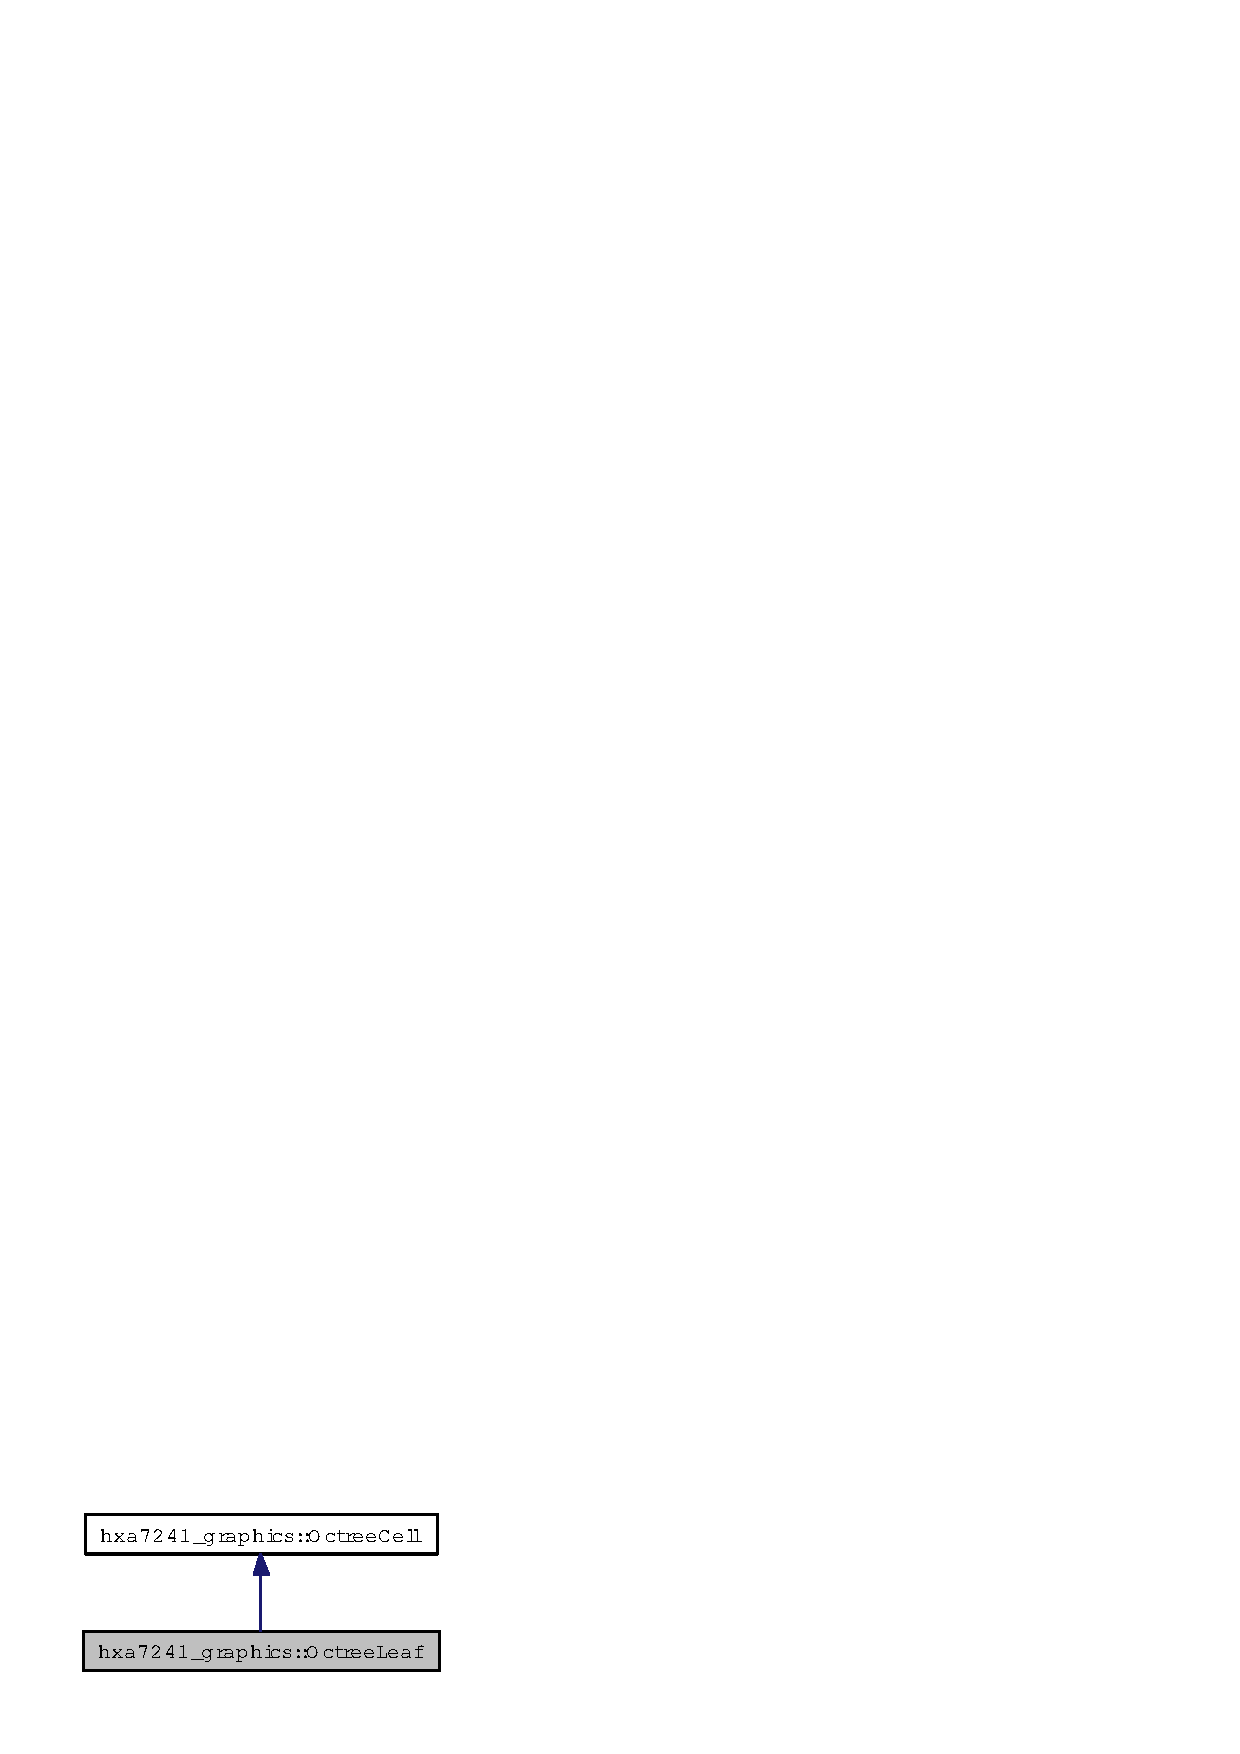
\includegraphics[width=107pt]{classhxa7241__graphics_1_1OctreeLeaf__inherit__graph}
\end{center}
\end{figure}
Collaboration diagram for hxa7241\_\-graphics::Octree\-Leaf:\begin{figure}[H]
\begin{center}
\leavevmode
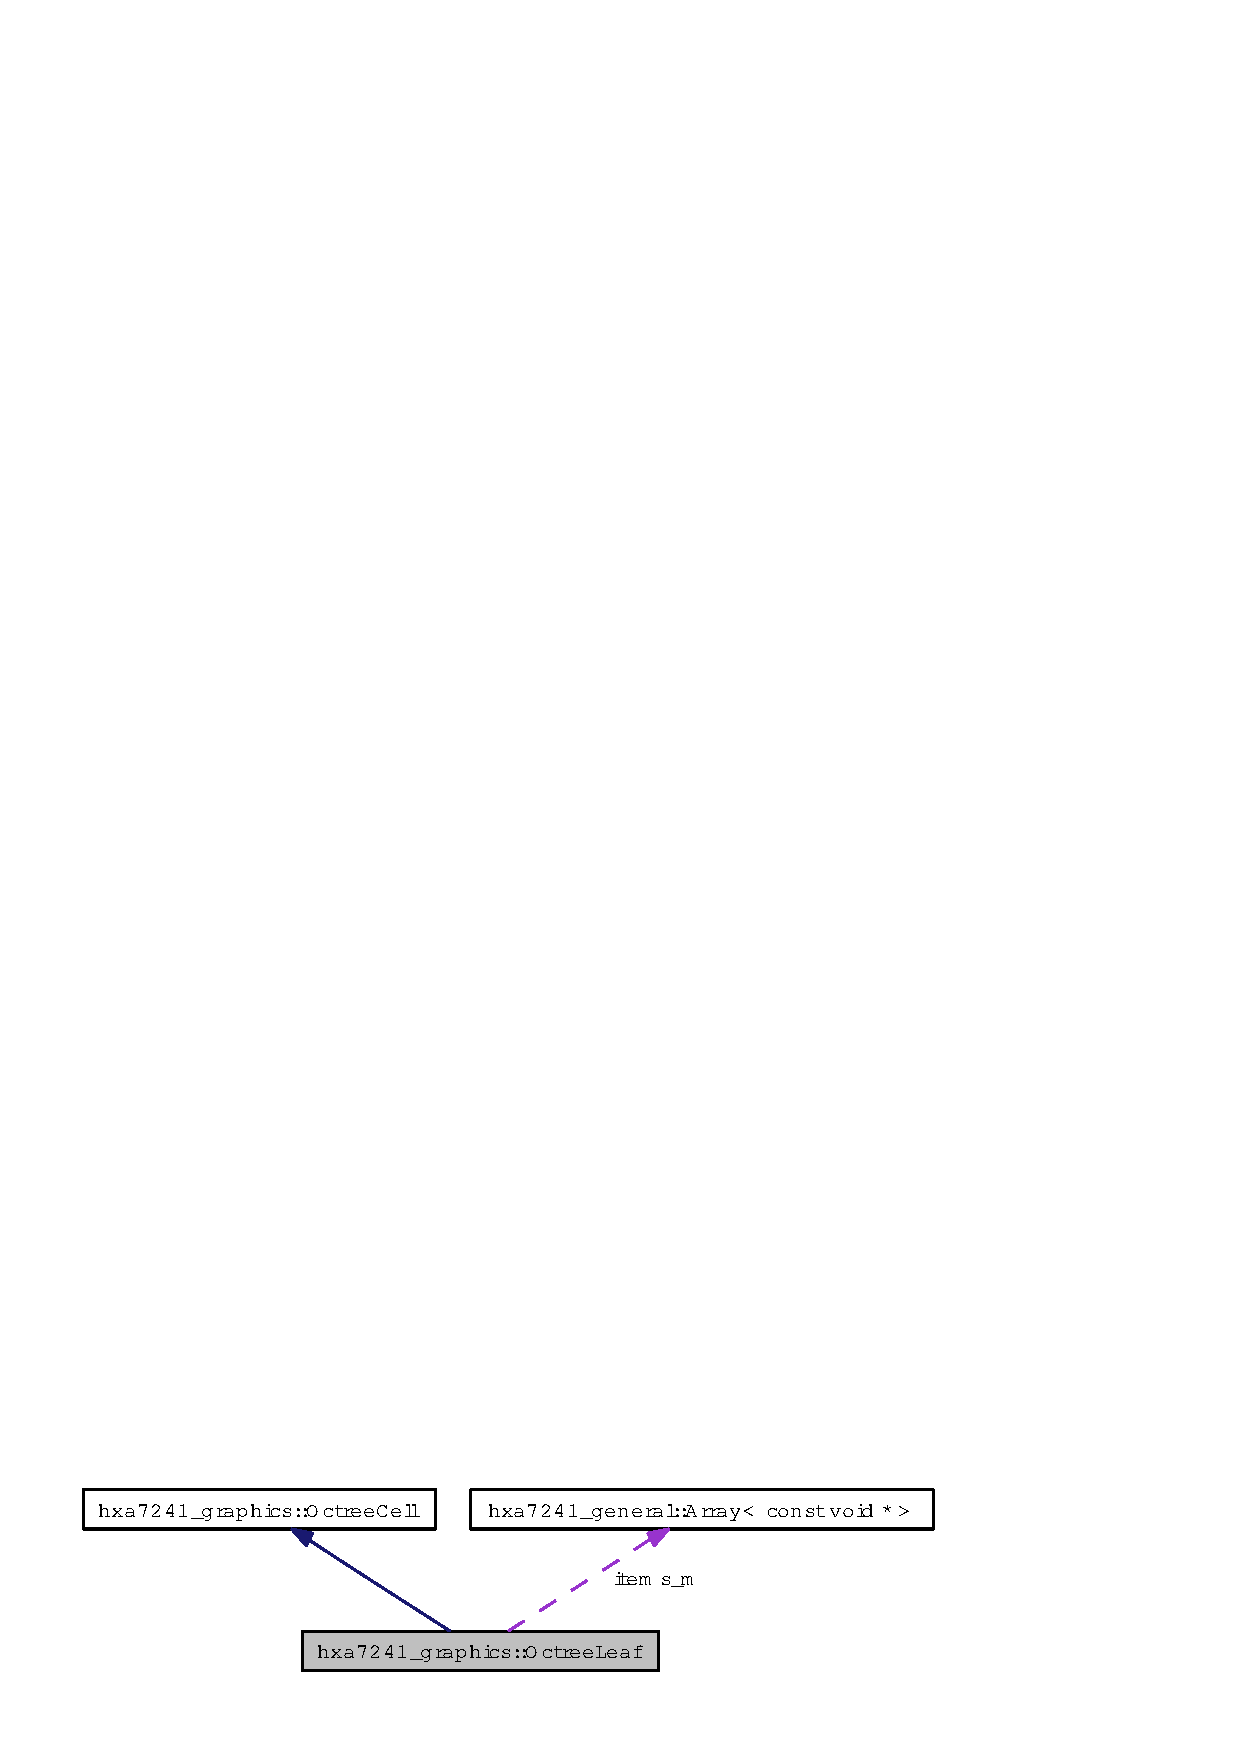
\includegraphics[width=226pt]{classhxa7241__graphics_1_1OctreeLeaf__coll__graph}
\end{center}
\end{figure}
\subsection*{Public Member Functions}
\begin{CompactItemize}
\item 
{\bf Octree\-Leaf} ()
\begin{CompactList}\small\item\em standard object services --------------------------------------------------- \item\end{CompactList}\item 
{\bf Octree\-Leaf} (const {\bf Octree\-Leaf} $\ast$const leafs[8])
\item 
virtual {\bf $\sim$Octree\-Leaf} ()
\item 
{\bf Octree\-Leaf} (const {\bf Octree\-Leaf} \&)
\item 
{\bf Octree\-Leaf} \& {\bf operator=} (const {\bf Octree\-Leaf} \&)
\item 
virtual void {\bf insert} (const {\bf Octree\-Data} \&this\-Data, {\bf Octree\-Cell} $\ast$\&p\-This, const void $\ast$p\-Item, const {\bf Octree\-Agent\-V} \&agent)
\begin{CompactList}\small\item\em commands ------------------------------------------------------------------- \item\end{CompactList}\item 
virtual bool {\bf remove} ({\bf Octree\-Cell} $\ast$\&p\-This, const void $\ast$p\-Item, const dword max\-Items\-Per\-Cell, dword \&item\-Count)
\item 
virtual void {\bf visit} (const {\bf Octree\-Data} \&this\-Data, {\bf Octree\-Visitor\-V} \&visitor) const
\begin{CompactList}\small\item\em queries -------------------------------------------------------------------- \item\end{CompactList}\item 
virtual {\bf Octree\-Cell} $\ast$ {\bf clone} () const
\item 
virtual void {\bf get\-Info} (dword \&byte\-Size, dword \&leaf\-Count, dword \&item\-Count, dword \&max\-Depth) const
\end{CompactItemize}
\subsection*{Static Public Member Functions}
\begin{CompactItemize}
\item 
static void {\bf insert\-Maybe\-Create} (const {\bf Octree\-Data} \&cell\-Data, {\bf Octree\-Cell} $\ast$\&p\-Cell, const void $\ast$p\-Item, const {\bf Octree\-Agent\-V} \&agent)
\begin{CompactList}\small\item\em statics -------------------------------------------------------------------- \item\end{CompactList}\end{CompactItemize}


\subsection{Detailed Description}
Outer node implementation of an octree cell.\par
\par


Stores pointers to items. 



\subsection{Constructor \& Destructor Documentation}
\index{hxa7241_graphics::OctreeLeaf@{hxa7241\_\-graphics::Octree\-Leaf}!OctreeLeaf@{OctreeLeaf}}
\index{OctreeLeaf@{OctreeLeaf}!hxa7241_graphics::OctreeLeaf@{hxa7241\_\-graphics::Octree\-Leaf}}
\subsubsection{\setlength{\rightskip}{0pt plus 5cm}Octree\-Leaf::Octree\-Leaf ()}\label{classhxa7241__graphics_1_1OctreeLeaf_dd1abe428a1cc09406717695800fec85}


standard object services --------------------------------------------------- 

\index{hxa7241_graphics::OctreeLeaf@{hxa7241\_\-graphics::Octree\-Leaf}!OctreeLeaf@{OctreeLeaf}}
\index{OctreeLeaf@{OctreeLeaf}!hxa7241_graphics::OctreeLeaf@{hxa7241\_\-graphics::Octree\-Leaf}}
\subsubsection{\setlength{\rightskip}{0pt plus 5cm}Octree\-Leaf::Octree\-Leaf (const {\bf Octree\-Leaf} $\ast$const {\em leafs}[8])}\label{classhxa7241__graphics_1_1OctreeLeaf_0add1cd96cfc5e7c8c632ebf79589fa2}


\index{hxa7241_graphics::OctreeLeaf@{hxa7241\_\-graphics::Octree\-Leaf}!~OctreeLeaf@{$\sim$OctreeLeaf}}
\index{~OctreeLeaf@{$\sim$OctreeLeaf}!hxa7241_graphics::OctreeLeaf@{hxa7241\_\-graphics::Octree\-Leaf}}
\subsubsection{\setlength{\rightskip}{0pt plus 5cm}Octree\-Leaf::$\sim$Octree\-Leaf ()\hspace{0.3cm}{\tt  [virtual]}}\label{classhxa7241__graphics_1_1OctreeLeaf_f75ac490fc5cbc56132ed5c99533c13b}


\index{hxa7241_graphics::OctreeLeaf@{hxa7241\_\-graphics::Octree\-Leaf}!OctreeLeaf@{OctreeLeaf}}
\index{OctreeLeaf@{OctreeLeaf}!hxa7241_graphics::OctreeLeaf@{hxa7241\_\-graphics::Octree\-Leaf}}
\subsubsection{\setlength{\rightskip}{0pt plus 5cm}Octree\-Leaf::Octree\-Leaf (const {\bf Octree\-Leaf} \&)}\label{classhxa7241__graphics_1_1OctreeLeaf_5784082a1e502115c9660d01781c5805}




\subsection{Member Function Documentation}
\index{hxa7241_graphics::OctreeLeaf@{hxa7241\_\-graphics::Octree\-Leaf}!operator=@{operator=}}
\index{operator=@{operator=}!hxa7241_graphics::OctreeLeaf@{hxa7241\_\-graphics::Octree\-Leaf}}
\subsubsection{\setlength{\rightskip}{0pt plus 5cm}{\bf Octree\-Leaf} \& Octree\-Leaf::operator= (const {\bf Octree\-Leaf} \&)}\label{classhxa7241__graphics_1_1OctreeLeaf_793614a3e6316183ce641d90be1a5bc4}


\index{hxa7241_graphics::OctreeLeaf@{hxa7241\_\-graphics::Octree\-Leaf}!insert@{insert}}
\index{insert@{insert}!hxa7241_graphics::OctreeLeaf@{hxa7241\_\-graphics::Octree\-Leaf}}
\subsubsection{\setlength{\rightskip}{0pt plus 5cm}void Octree\-Leaf::insert (const {\bf Octree\-Data} \& {\em this\-Data}, {\bf Octree\-Cell} $\ast$\& {\em p\-This}, const void $\ast$ {\em p\-Item}, const {\bf Octree\-Agent\-V} \& {\em agent})\hspace{0.3cm}{\tt  [virtual]}}\label{classhxa7241__graphics_1_1OctreeLeaf_7c6393f830a72b179948dd5bee97eeb4}


commands ------------------------------------------------------------------- 



Implements {\bf hxa7241\_\-graphics::Octree\-Cell} \doxyref{}{p.}{classhxa7241__graphics_1_1OctreeCell_0cf5936ffeaca906be184ac654cd8053}.\index{hxa7241_graphics::OctreeLeaf@{hxa7241\_\-graphics::Octree\-Leaf}!remove@{remove}}
\index{remove@{remove}!hxa7241_graphics::OctreeLeaf@{hxa7241\_\-graphics::Octree\-Leaf}}
\subsubsection{\setlength{\rightskip}{0pt plus 5cm}bool Octree\-Leaf::remove ({\bf Octree\-Cell} $\ast$\& {\em p\-This}, const void $\ast$ {\em p\-Item}, const dword {\em max\-Items\-Per\-Cell}, dword \& {\em item\-Count})\hspace{0.3cm}{\tt  [virtual]}}\label{classhxa7241__graphics_1_1OctreeLeaf_64a170120344343a7f5309248aba2ab7}




Implements {\bf hxa7241\_\-graphics::Octree\-Cell} \doxyref{}{p.}{classhxa7241__graphics_1_1OctreeCell_74c11f0b4d5ef93959253206c3816417}.\index{hxa7241_graphics::OctreeLeaf@{hxa7241\_\-graphics::Octree\-Leaf}!visit@{visit}}
\index{visit@{visit}!hxa7241_graphics::OctreeLeaf@{hxa7241\_\-graphics::Octree\-Leaf}}
\subsubsection{\setlength{\rightskip}{0pt plus 5cm}void Octree\-Leaf::visit (const {\bf Octree\-Data} \& {\em this\-Data}, {\bf Octree\-Visitor\-V} \& {\em visitor}) const\hspace{0.3cm}{\tt  [virtual]}}\label{classhxa7241__graphics_1_1OctreeLeaf_4dc0120fbd3d27f6628a507faf13d323}


queries -------------------------------------------------------------------- 



Implements {\bf hxa7241\_\-graphics::Octree\-Cell} \doxyref{}{p.}{classhxa7241__graphics_1_1OctreeCell_e0998c3188914314451880d40ebd1c35}.\index{hxa7241_graphics::OctreeLeaf@{hxa7241\_\-graphics::Octree\-Leaf}!clone@{clone}}
\index{clone@{clone}!hxa7241_graphics::OctreeLeaf@{hxa7241\_\-graphics::Octree\-Leaf}}
\subsubsection{\setlength{\rightskip}{0pt plus 5cm}{\bf Octree\-Cell} $\ast$ Octree\-Leaf::clone () const\hspace{0.3cm}{\tt  [virtual]}}\label{classhxa7241__graphics_1_1OctreeLeaf_0908765dbe95af75036abc65380a3aa8}




Implements {\bf hxa7241\_\-graphics::Octree\-Cell} \doxyref{}{p.}{classhxa7241__graphics_1_1OctreeCell_6f10b6cebce798d4a3e96b8822584774}.\index{hxa7241_graphics::OctreeLeaf@{hxa7241\_\-graphics::Octree\-Leaf}!getInfo@{getInfo}}
\index{getInfo@{getInfo}!hxa7241_graphics::OctreeLeaf@{hxa7241\_\-graphics::Octree\-Leaf}}
\subsubsection{\setlength{\rightskip}{0pt plus 5cm}void Octree\-Leaf::get\-Info (dword \& {\em byte\-Size}, dword \& {\em leaf\-Count}, dword \& {\em item\-Count}, dword \& {\em max\-Depth}) const\hspace{0.3cm}{\tt  [virtual]}}\label{classhxa7241__graphics_1_1OctreeLeaf_ff8e9556edcae39b2d4fbd2db1d37b4f}




Implements {\bf hxa7241\_\-graphics::Octree\-Cell} \doxyref{}{p.}{classhxa7241__graphics_1_1OctreeCell_d8b69169addb924c9ec3bb6ae70a932f}.\index{hxa7241_graphics::OctreeLeaf@{hxa7241\_\-graphics::Octree\-Leaf}!insertMaybeCreate@{insertMaybeCreate}}
\index{insertMaybeCreate@{insertMaybeCreate}!hxa7241_graphics::OctreeLeaf@{hxa7241\_\-graphics::Octree\-Leaf}}
\subsubsection{\setlength{\rightskip}{0pt plus 5cm}void Octree\-Leaf::insert\-Maybe\-Create (const {\bf Octree\-Data} \& {\em cell\-Data}, {\bf Octree\-Cell} $\ast$\& {\em p\-Cell}, const void $\ast$ {\em p\-Item}, const {\bf Octree\-Agent\-V} \& {\em agent})\hspace{0.3cm}{\tt  [static]}}\label{classhxa7241__graphics_1_1OctreeLeaf_64ce64675db0b34d5207497d42a39a5b}


statics -------------------------------------------------------------------- 



The documentation for this class was generated from the following files:\begin{CompactItemize}
\item 
{\bf Octree\-Implementation.h}\item 
{\bf Octree\-Implementation.cc}\end{CompactItemize}

\section{hxa7241\_\-graphics::Octree\-Root Class Reference}
\label{classhxa7241__graphics_1_1OctreeRoot}\index{hxa7241_graphics::OctreeRoot@{hxa7241\_\-graphics::OctreeRoot}}
{\tt \#include $<$Octree\-Implementation.h$>$}

Collaboration diagram for hxa7241\_\-graphics::Octree\-Root:\begin{figure}[H]
\begin{center}
\leavevmode
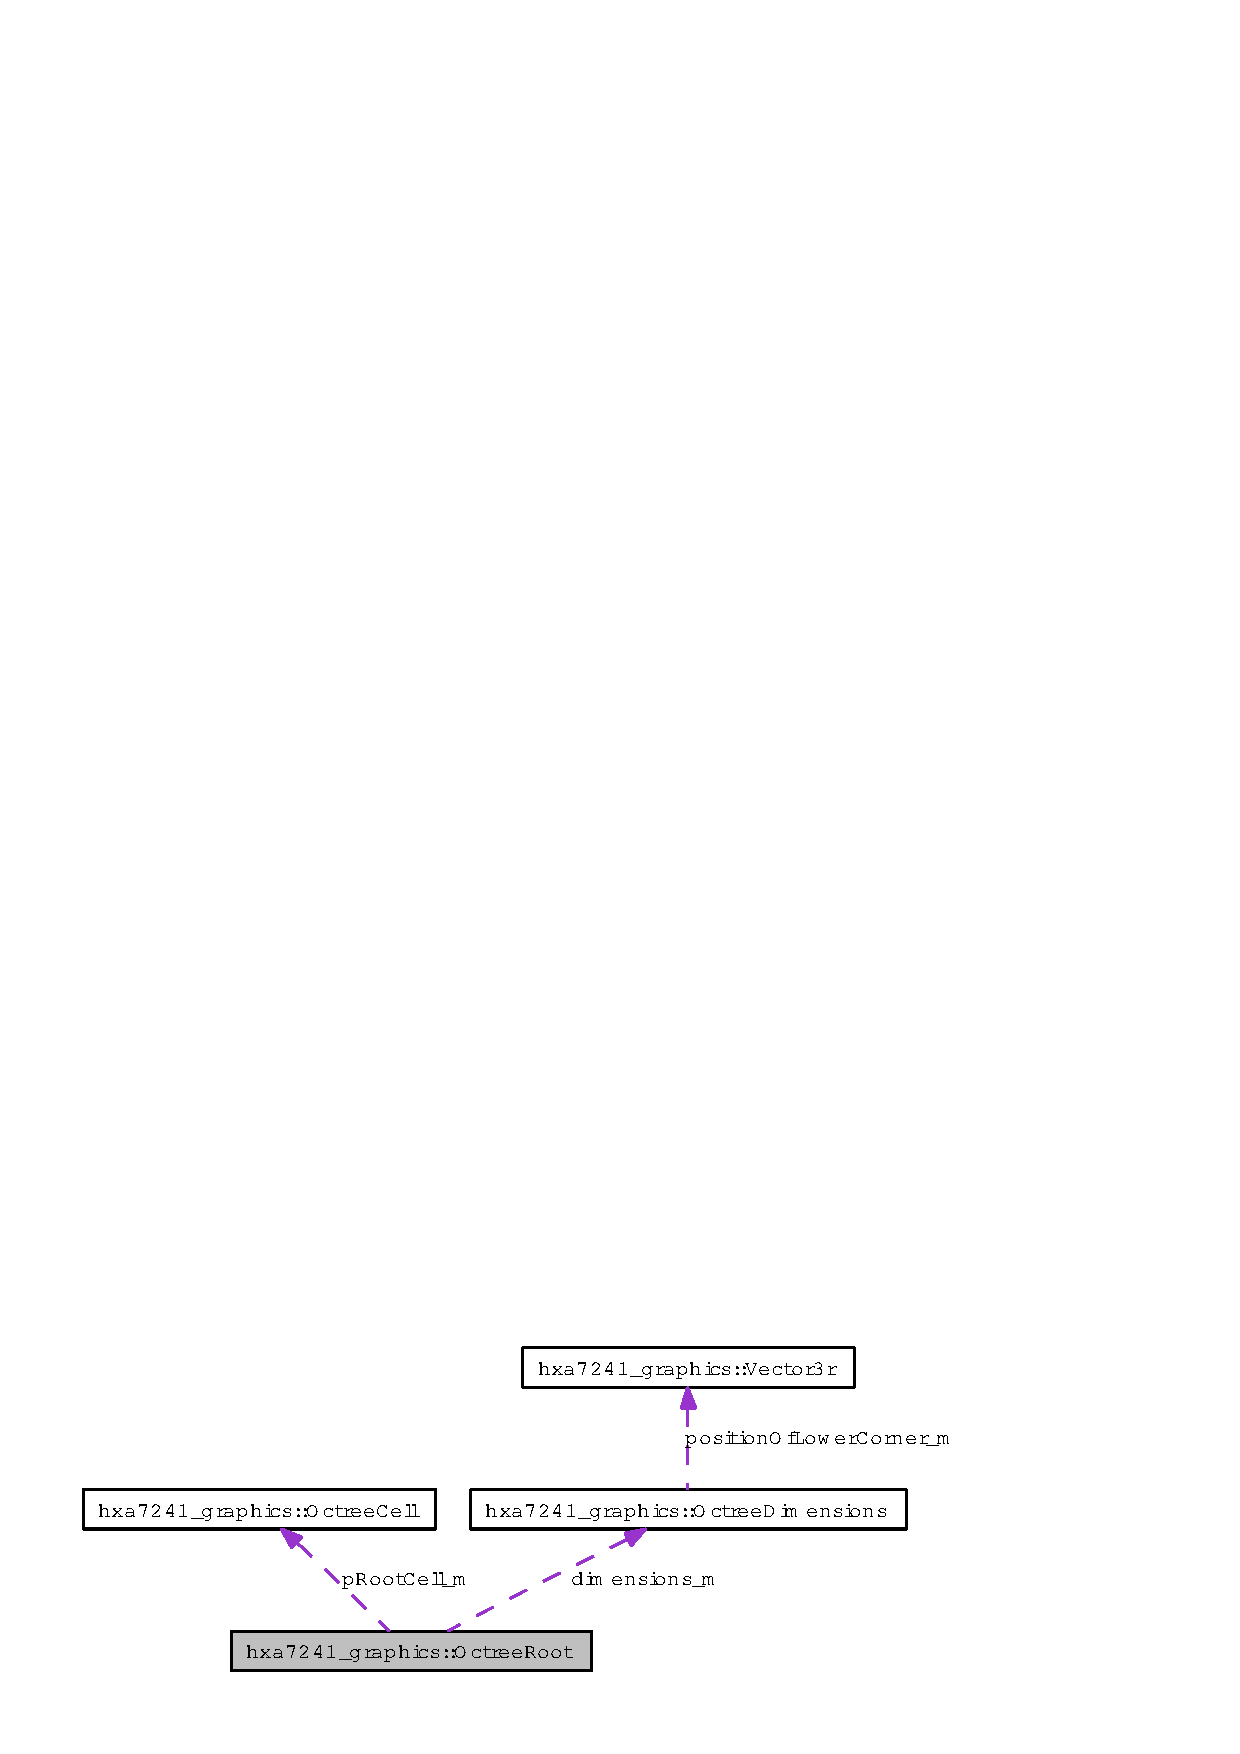
\includegraphics[width=232pt]{classhxa7241__graphics_1_1OctreeRoot__coll__graph}
\end{center}
\end{figure}
\subsection*{Public Member Functions}
\begin{CompactItemize}
\item 
{\bf Octree\-Root} (const {\bf Vector3r} \&position, real size\-Of\-Cube, dword max\-Items\-Per\-Cell, dword max\-Level\-Count, real min\-Cell\-Size)
\begin{CompactList}\small\item\em standard object services --------------------------------------------------- \item\end{CompactList}\item 
{\bf $\sim$Octree\-Root} ()
\item 
{\bf Octree\-Root} (const {\bf Octree\-Root} \&)
\item 
{\bf Octree\-Root} \& {\bf operator=} (const {\bf Octree\-Root} \&)
\item 
bool {\bf insert} (const void $\ast$p\-Item, const {\bf Octree\-Agent\-V} \&agent)
\begin{CompactList}\small\item\em commands ------------------------------------------------------------------- \item\end{CompactList}\item 
bool {\bf remove} (const void $\ast$p\-Item, const {\bf Octree\-Agent\-V} \&agent)
\item 
void {\bf visit} ({\bf Octree\-Visitor\-V} \&visitor) const
\begin{CompactList}\small\item\em queries -------------------------------------------------------------------- \item\end{CompactList}\item 
bool {\bf is\-Empty} () const
\item 
void {\bf get\-Info} (dword root\-Wrapper\-Byte\-Size, dword \&byte\-Size, dword \&leaf\-Count, dword \&item\-Count, dword \&max\-Depth) const
\item 
const {\bf Vector3r} \& {\bf get\-Position} () const
\item 
real {\bf get\-Size} () const
\item 
dword {\bf get\-Max\-Item\-Count\-Per\-Cell} () const
\item 
dword {\bf get\-Max\-Level\-Count} () const
\item 
real {\bf get\-Min\-Cell\-Size} () const
\end{CompactItemize}
\subsection*{Static Public Member Functions}
\begin{CompactItemize}
\item 
static void {\bf continue\-Visit} (const {\bf Octree\-Cell} $\ast$p\-Root\-Cell, const {\bf Octree\-Data} \&octree\-Data, {\bf Octree\-Visitor\-V} \&visitor)
\begin{CompactList}\small\item\em statics -------------------------------------------------------------------- \item\end{CompactList}\end{CompactItemize}


\subsection{Detailed Description}
Implementation class for the \doxyref{Octree}{p.}{classhxa7241__graphics_1_1Octree} template.

p\-Root\-Cell\_\-m can be null, or point to an \doxyref{Octree\-Cell}{p.}{classhxa7241__graphics_1_1OctreeCell} instance.\par
\par


At construction, p\-Root\-Cell\_\-m is set to a legal value.\par
 At destruction, p\-Root\-Cell\_\-m is deleted.\par
 Whenever p\-Root\-Cell\_\-m is modified, it must be deleted then set to a legal value.\par
 A legal value is: either 0, or the value from invocation of 'new'. 



\subsection{Constructor \& Destructor Documentation}
\index{hxa7241_graphics::OctreeRoot@{hxa7241\_\-graphics::Octree\-Root}!OctreeRoot@{OctreeRoot}}
\index{OctreeRoot@{OctreeRoot}!hxa7241_graphics::OctreeRoot@{hxa7241\_\-graphics::Octree\-Root}}
\subsubsection{\setlength{\rightskip}{0pt plus 5cm}Octree\-Root::Octree\-Root (const {\bf Vector3r} \& {\em position}, real {\em size\-Of\-Cube}, dword {\em max\-Items\-Per\-Cell}, dword {\em max\-Level\-Count}, real {\em min\-Cell\-Size})}\label{classhxa7241__graphics_1_1OctreeRoot_7a1c6a606e9adf05871c055b89d4374c}


standard object services --------------------------------------------------- 

\index{hxa7241_graphics::OctreeRoot@{hxa7241\_\-graphics::Octree\-Root}!~OctreeRoot@{$\sim$OctreeRoot}}
\index{~OctreeRoot@{$\sim$OctreeRoot}!hxa7241_graphics::OctreeRoot@{hxa7241\_\-graphics::Octree\-Root}}
\subsubsection{\setlength{\rightskip}{0pt plus 5cm}Octree\-Root::$\sim$Octree\-Root ()}\label{classhxa7241__graphics_1_1OctreeRoot_b39f0fcdc286c563692dc03a07668dc3}


\index{hxa7241_graphics::OctreeRoot@{hxa7241\_\-graphics::Octree\-Root}!OctreeRoot@{OctreeRoot}}
\index{OctreeRoot@{OctreeRoot}!hxa7241_graphics::OctreeRoot@{hxa7241\_\-graphics::Octree\-Root}}
\subsubsection{\setlength{\rightskip}{0pt plus 5cm}Octree\-Root::Octree\-Root (const {\bf Octree\-Root} \&)}\label{classhxa7241__graphics_1_1OctreeRoot_647330ec8bfeec42204deb11424a7a06}




\subsection{Member Function Documentation}
\index{hxa7241_graphics::OctreeRoot@{hxa7241\_\-graphics::Octree\-Root}!operator=@{operator=}}
\index{operator=@{operator=}!hxa7241_graphics::OctreeRoot@{hxa7241\_\-graphics::Octree\-Root}}
\subsubsection{\setlength{\rightskip}{0pt plus 5cm}{\bf Octree\-Root} \& Octree\-Root::operator= (const {\bf Octree\-Root} \&)}\label{classhxa7241__graphics_1_1OctreeRoot_4cb94840043915af398a92d7a5094ffb}


\index{hxa7241_graphics::OctreeRoot@{hxa7241\_\-graphics::Octree\-Root}!insert@{insert}}
\index{insert@{insert}!hxa7241_graphics::OctreeRoot@{hxa7241\_\-graphics::Octree\-Root}}
\subsubsection{\setlength{\rightskip}{0pt plus 5cm}bool Octree\-Root::insert (const void $\ast$ {\em p\-Item}, const {\bf Octree\-Agent\-V} \& {\em agent})}\label{classhxa7241__graphics_1_1OctreeRoot_78d548a33bfc453ad34bac28513975cc}


commands ------------------------------------------------------------------- 

\index{hxa7241_graphics::OctreeRoot@{hxa7241\_\-graphics::Octree\-Root}!remove@{remove}}
\index{remove@{remove}!hxa7241_graphics::OctreeRoot@{hxa7241\_\-graphics::Octree\-Root}}
\subsubsection{\setlength{\rightskip}{0pt plus 5cm}bool Octree\-Root::remove (const void $\ast$ {\em p\-Item}, const {\bf Octree\-Agent\-V} \& {\em agent})}\label{classhxa7241__graphics_1_1OctreeRoot_674a25660370049a0abc883b570fa0ea}


\index{hxa7241_graphics::OctreeRoot@{hxa7241\_\-graphics::Octree\-Root}!visit@{visit}}
\index{visit@{visit}!hxa7241_graphics::OctreeRoot@{hxa7241\_\-graphics::Octree\-Root}}
\subsubsection{\setlength{\rightskip}{0pt plus 5cm}void Octree\-Root::visit ({\bf Octree\-Visitor\-V} \& {\em visitor}) const}\label{classhxa7241__graphics_1_1OctreeRoot_b75c3b0cbf7424cf45b08b275bb6d4ce}


queries -------------------------------------------------------------------- 

\index{hxa7241_graphics::OctreeRoot@{hxa7241\_\-graphics::Octree\-Root}!isEmpty@{isEmpty}}
\index{isEmpty@{isEmpty}!hxa7241_graphics::OctreeRoot@{hxa7241\_\-graphics::Octree\-Root}}
\subsubsection{\setlength{\rightskip}{0pt plus 5cm}bool Octree\-Root::is\-Empty () const}\label{classhxa7241__graphics_1_1OctreeRoot_8eb4830e521b4b9ea9e926f42ee07887}


\index{hxa7241_graphics::OctreeRoot@{hxa7241\_\-graphics::Octree\-Root}!getInfo@{getInfo}}
\index{getInfo@{getInfo}!hxa7241_graphics::OctreeRoot@{hxa7241\_\-graphics::Octree\-Root}}
\subsubsection{\setlength{\rightskip}{0pt plus 5cm}void Octree\-Root::get\-Info (dword {\em root\-Wrapper\-Byte\-Size}, dword \& {\em byte\-Size}, dword \& {\em leaf\-Count}, dword \& {\em item\-Count}, dword \& {\em max\-Depth}) const}\label{classhxa7241__graphics_1_1OctreeRoot_f6d915235693b71c06686144cd224e27}


\index{hxa7241_graphics::OctreeRoot@{hxa7241\_\-graphics::Octree\-Root}!getPosition@{getPosition}}
\index{getPosition@{getPosition}!hxa7241_graphics::OctreeRoot@{hxa7241\_\-graphics::Octree\-Root}}
\subsubsection{\setlength{\rightskip}{0pt plus 5cm}const {\bf Vector3r} \& Octree\-Root::get\-Position () const}\label{classhxa7241__graphics_1_1OctreeRoot_200ff7f2e2d3213437535f07021dbdfe}


\index{hxa7241_graphics::OctreeRoot@{hxa7241\_\-graphics::Octree\-Root}!getSize@{getSize}}
\index{getSize@{getSize}!hxa7241_graphics::OctreeRoot@{hxa7241\_\-graphics::Octree\-Root}}
\subsubsection{\setlength{\rightskip}{0pt plus 5cm}real Octree\-Root::get\-Size () const}\label{classhxa7241__graphics_1_1OctreeRoot_877a933a326a54cc5e3dac03fa40cd06}


\index{hxa7241_graphics::OctreeRoot@{hxa7241\_\-graphics::Octree\-Root}!getMaxItemCountPerCell@{getMaxItemCountPerCell}}
\index{getMaxItemCountPerCell@{getMaxItemCountPerCell}!hxa7241_graphics::OctreeRoot@{hxa7241\_\-graphics::Octree\-Root}}
\subsubsection{\setlength{\rightskip}{0pt plus 5cm}dword Octree\-Root::get\-Max\-Item\-Count\-Per\-Cell () const}\label{classhxa7241__graphics_1_1OctreeRoot_1ff78be3bcf149987d60b49f57700ad1}


\index{hxa7241_graphics::OctreeRoot@{hxa7241\_\-graphics::Octree\-Root}!getMaxLevelCount@{getMaxLevelCount}}
\index{getMaxLevelCount@{getMaxLevelCount}!hxa7241_graphics::OctreeRoot@{hxa7241\_\-graphics::Octree\-Root}}
\subsubsection{\setlength{\rightskip}{0pt plus 5cm}dword Octree\-Root::get\-Max\-Level\-Count () const}\label{classhxa7241__graphics_1_1OctreeRoot_b4048fa55e9222bbf3716faeed3b595a}


\index{hxa7241_graphics::OctreeRoot@{hxa7241\_\-graphics::Octree\-Root}!getMinCellSize@{getMinCellSize}}
\index{getMinCellSize@{getMinCellSize}!hxa7241_graphics::OctreeRoot@{hxa7241\_\-graphics::Octree\-Root}}
\subsubsection{\setlength{\rightskip}{0pt plus 5cm}real Octree\-Root::get\-Min\-Cell\-Size () const}\label{classhxa7241__graphics_1_1OctreeRoot_a061a8e2cc29b7674fe0522e9c4b36c6}


\index{hxa7241_graphics::OctreeRoot@{hxa7241\_\-graphics::Octree\-Root}!continueVisit@{continueVisit}}
\index{continueVisit@{continueVisit}!hxa7241_graphics::OctreeRoot@{hxa7241\_\-graphics::Octree\-Root}}
\subsubsection{\setlength{\rightskip}{0pt plus 5cm}void Octree\-Root::continue\-Visit (const {\bf Octree\-Cell} $\ast$ {\em p\-Root\-Cell}, const {\bf Octree\-Data} \& {\em octree\-Data}, {\bf Octree\-Visitor\-V} \& {\em visitor})\hspace{0.3cm}{\tt  [static]}}\label{classhxa7241__graphics_1_1OctreeRoot_886f24f550bc0d50fb64c4b0c6de64f9}


statics -------------------------------------------------------------------- 



The documentation for this class was generated from the following files:\begin{CompactItemize}
\item 
{\bf Octree\-Implementation.h}\item 
{\bf Octree\-Implementation.cc}\end{CompactItemize}

\section{hxa7241\_\-graphics::Octree\-Visitor$<$ TYPE $>$ Class Template Reference}
\label{classhxa7241__graphics_1_1OctreeVisitor}\index{hxa7241_graphics::OctreeVisitor@{hxa7241\_\-graphics::OctreeVisitor}}
{\tt \#include $<$Octree.h$>$}

Inheritance diagram for hxa7241\_\-graphics::Octree\-Visitor$<$ TYPE $>$:\begin{figure}[H]
\begin{center}
\leavevmode
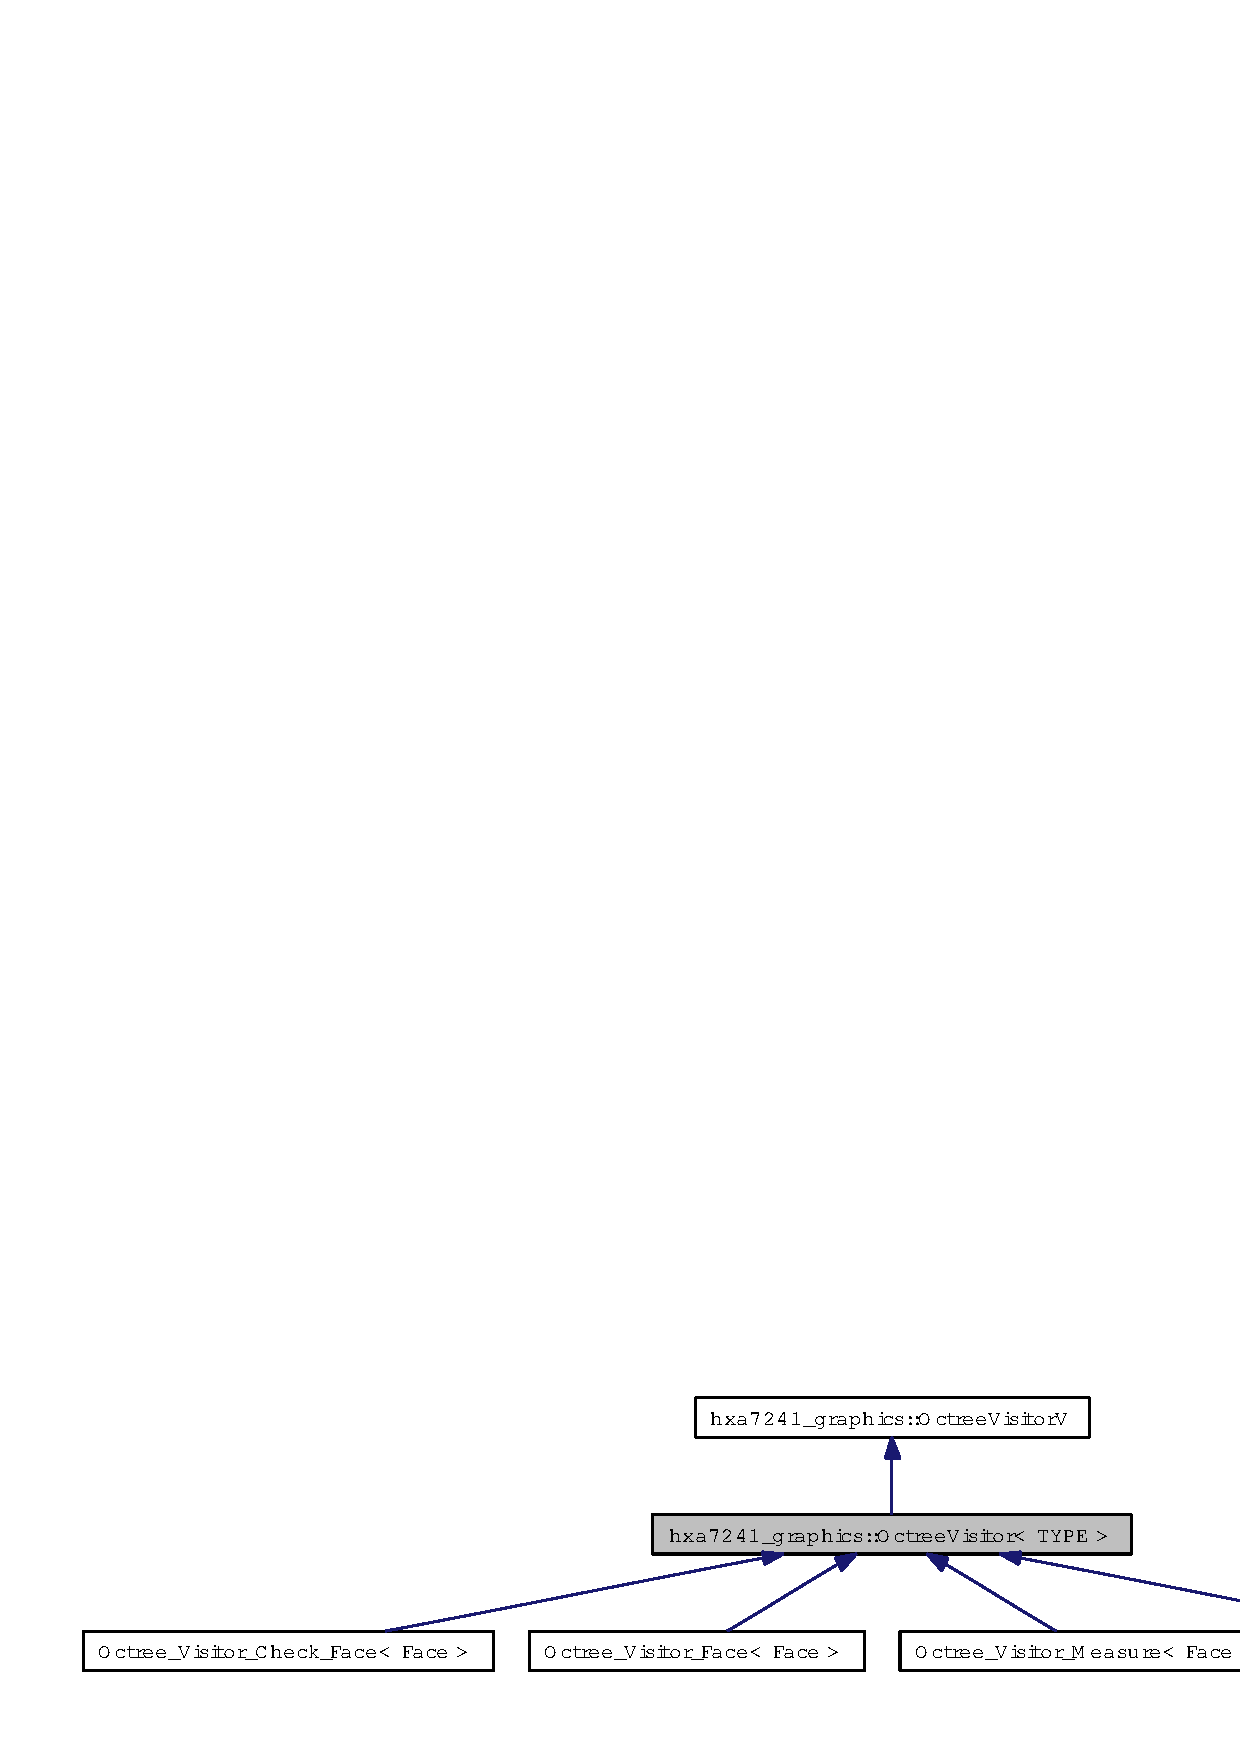
\includegraphics[width=404pt]{classhxa7241__graphics_1_1OctreeVisitor__inherit__graph}
\end{center}
\end{figure}
Collaboration diagram for hxa7241\_\-graphics::Octree\-Visitor$<$ TYPE $>$:\begin{figure}[H]
\begin{center}
\leavevmode
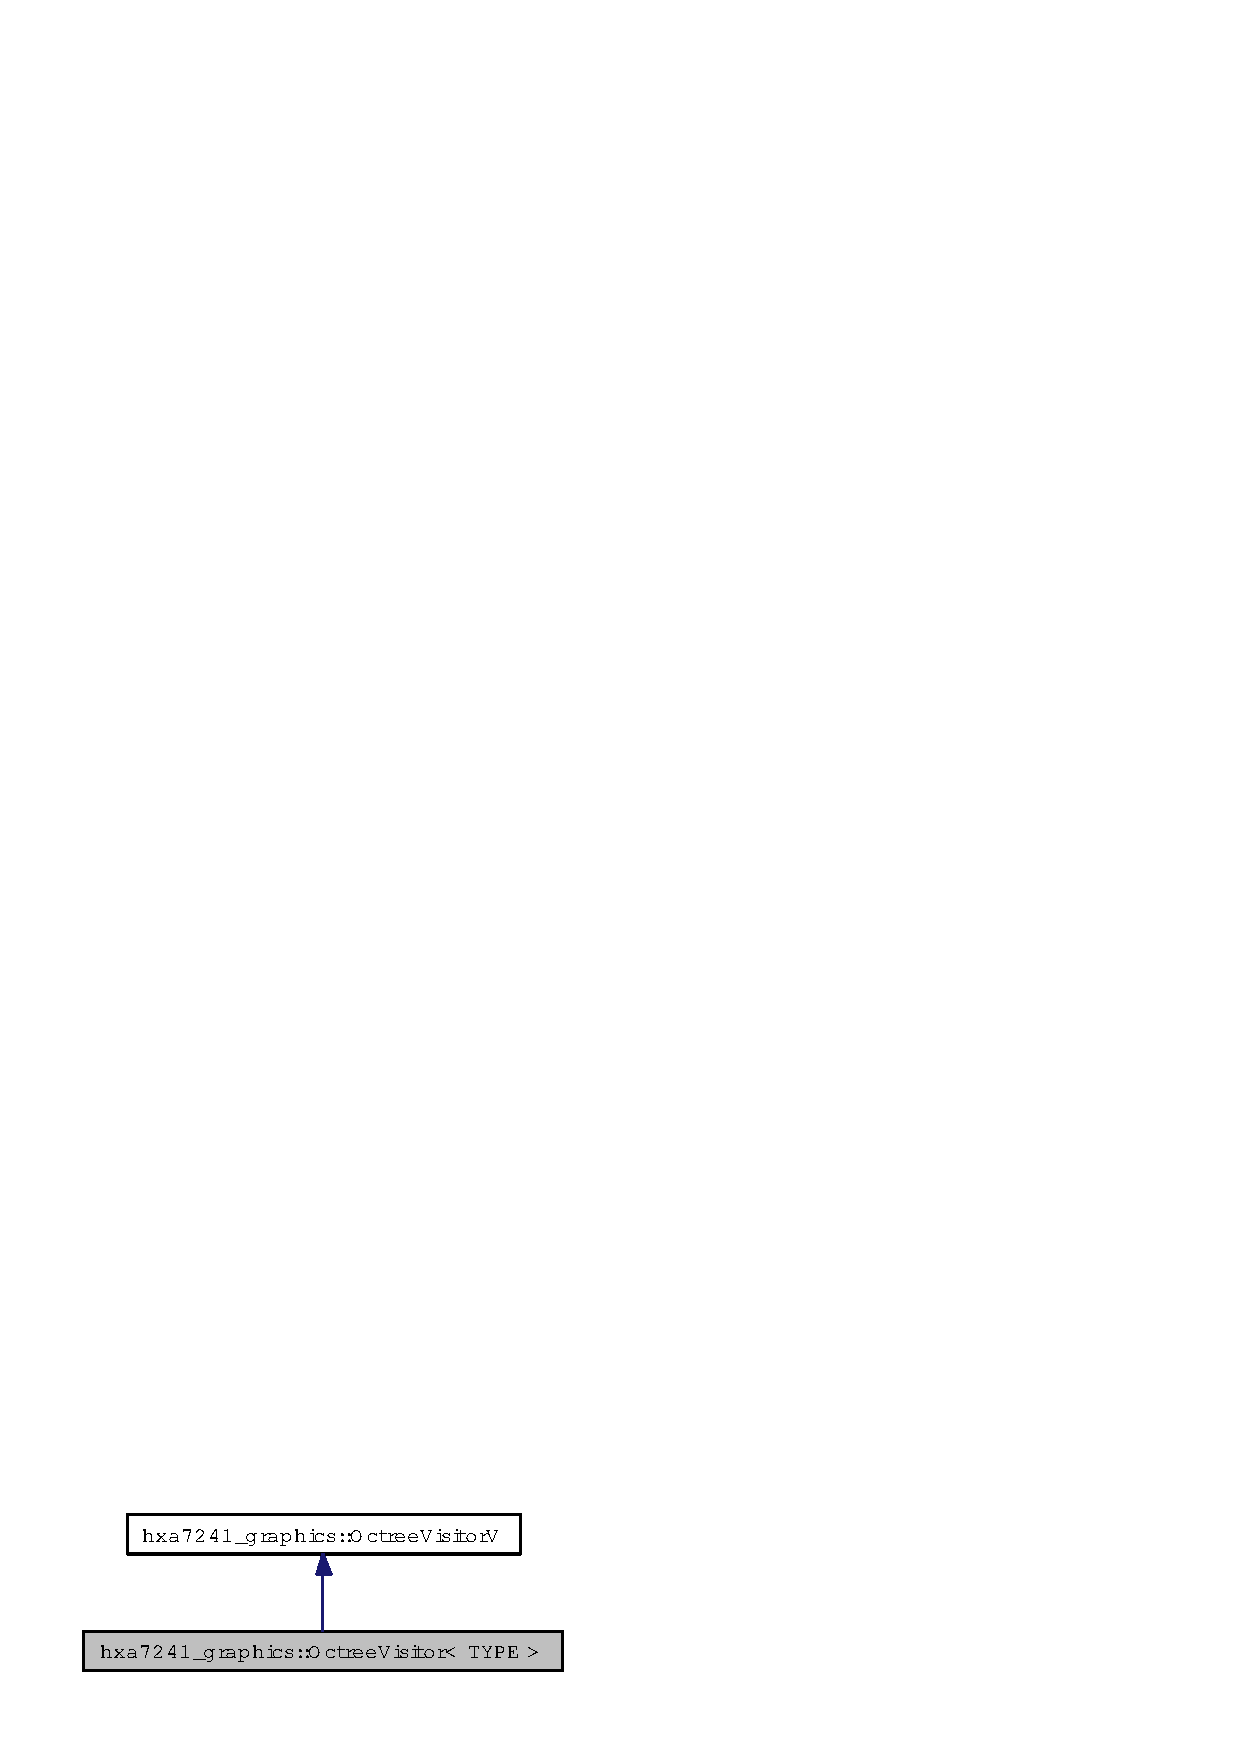
\includegraphics[width=137pt]{classhxa7241__graphics_1_1OctreeVisitor__coll__graph}
\end{center}
\end{figure}
\subsection*{Public Member Functions}
\begin{CompactItemize}
\item 
virtual {\bf $\sim$Octree\-Visitor} ()
\item 
virtual void {\bf visit\-Root\-V} (const {\bf Octree\-Cell} $\ast$p\-Root\-Cell, const {\bf Octree\-Data} \&octree\-Data)
\begin{CompactList}\small\item\em void-to-type forwarders \item\end{CompactList}\item 
virtual void {\bf visit\-Branch\-V} (const {\bf Octree\-Cell} $\ast$sub\-Cells[8], const {\bf Octree\-Data} \&octree\-Data)
\item 
virtual void {\bf visit\-Leaf\-V} (const {\bf Array}$<$ const void $\ast$ $>$ \&items, const {\bf Octree\-Data} \&octree\-Data)
\end{CompactItemize}
\subsection*{Protected Member Functions}
\begin{CompactItemize}
\item 
{\bf Octree\-Visitor} ()
\begin{CompactList}\small\item\em standard object services --------------------------------------------------- \item\end{CompactList}\item 
virtual void {\bf visit\-Root} (const {\bf Octree\-Cell} $\ast$p\-Root\-Cell, const {\bf Octree\-Data} \&octree\-Data)=0
\begin{CompactList}\small\item\em commands ------------------------------------------------------------------- \item\end{CompactList}\item 
virtual void {\bf visit\-Branch} (const {\bf Octree\-Cell} $\ast$sub\-Cells[8], const {\bf Octree\-Data} \&octree\-Data)=0
\item 
virtual void {\bf visit\-Leaf} (const {\bf Array}$<$ const TYPE $\ast$ $>$ \&items, const {\bf Octree\-Data} \&octree\-Data)=0
\end{CompactItemize}


\subsection{Detailed Description}
\subsubsection*{template$<$class TYPE$>$ class hxa7241\_\-graphics::Octree\-Visitor$<$ TYPE $>$}

Visitor abstract base, for client use with \doxyref{Octree}{p.}{classhxa7241__graphics_1_1Octree}.\par
\par


Client of \doxyref{Octree}{p.}{classhxa7241__graphics_1_1Octree} must define a concrete derivative of Octree\-Visitor$<$Item\-Type$>$.\par
\par


This is a reversal of the Visitor pattern: it allows an operation to be performed with the \doxyref{Octree}{p.}{classhxa7241__graphics_1_1Octree}, except the \doxyref{Octree}{p.}{classhxa7241__graphics_1_1Octree} is merely read from and it is the visitor that is modified.\par
\par


The visit methods are called by the tree nodes during the visit operation. The parameters supply the cell and boundary info. The implementation can call visit on the supplied cell.\par
\par


The implementation of visit\-Branch needs to make the \doxyref{Octree\-Data}{p.}{classhxa7241__graphics_1_1OctreeData} to be given in each call of visit.

Subcell numbering: \small\begin{alltt}
    y z       6 7
    |/   2 3  4 5
     -x  0 1
 \end{alltt}
\normalsize 
 in binary: \small\begin{alltt}
    y z           110 111
    |/   010 011  100 101
     -x  000 001
 \end{alltt}
\normalsize 


The \_\-\_\-\_\-V methods simply apply a type-cast to void$\ast$s and forward to their abstract counterparts.\par
\par
 



\subsection{Constructor \& Destructor Documentation}
\index{hxa7241_graphics::OctreeVisitor@{hxa7241\_\-graphics::Octree\-Visitor}!OctreeVisitor@{OctreeVisitor}}
\index{OctreeVisitor@{OctreeVisitor}!hxa7241_graphics::OctreeVisitor@{hxa7241\_\-graphics::Octree\-Visitor}}
\subsubsection{\setlength{\rightskip}{0pt plus 5cm}template$<$class TYPE$>$ {\bf hxa7241\_\-graphics::Octree\-Visitor}$<$ TYPE $>$::{\bf Octree\-Visitor} ()\hspace{0.3cm}{\tt  [inline, protected]}}\label{classhxa7241__graphics_1_1OctreeVisitor_7055025ef0b10d6f6f35e636f62de785}


standard object services --------------------------------------------------- 

\index{hxa7241_graphics::OctreeVisitor@{hxa7241\_\-graphics::Octree\-Visitor}!~OctreeVisitor@{$\sim$OctreeVisitor}}
\index{~OctreeVisitor@{$\sim$OctreeVisitor}!hxa7241_graphics::OctreeVisitor@{hxa7241\_\-graphics::Octree\-Visitor}}
\subsubsection{\setlength{\rightskip}{0pt plus 5cm}template$<$class TYPE$>$ virtual {\bf hxa7241\_\-graphics::Octree\-Visitor}$<$ TYPE $>$::$\sim${\bf Octree\-Visitor} ()\hspace{0.3cm}{\tt  [inline, virtual]}}\label{classhxa7241__graphics_1_1OctreeVisitor_35e6ed22803d5fbc29bb2994a0bf9fe0}




\subsection{Member Function Documentation}
\index{hxa7241_graphics::OctreeVisitor@{hxa7241\_\-graphics::Octree\-Visitor}!visitRootV@{visitRootV}}
\index{visitRootV@{visitRootV}!hxa7241_graphics::OctreeVisitor@{hxa7241\_\-graphics::Octree\-Visitor}}
\subsubsection{\setlength{\rightskip}{0pt plus 5cm}template$<$class TYPE$>$ void {\bf hxa7241\_\-graphics::Octree\-Visitor}$<$ TYPE $>$::visit\-Root\-V (const {\bf Octree\-Cell} $\ast$ {\em p\-Root\-Cell}, const {\bf Octree\-Data} \& {\em octree\-Data})\hspace{0.3cm}{\tt  [inline, virtual]}}\label{classhxa7241__graphics_1_1OctreeVisitor_61cd041a87e104914494e99b5e9e7d8c}


void-to-type forwarders 



Implements {\bf hxa7241\_\-graphics::Octree\-Visitor\-V} \doxyref{}{p.}{classhxa7241__graphics_1_1OctreeVisitorV_ed002d0f93c17840c621f5840cf986e4}.\index{hxa7241_graphics::OctreeVisitor@{hxa7241\_\-graphics::Octree\-Visitor}!visitBranchV@{visitBranchV}}
\index{visitBranchV@{visitBranchV}!hxa7241_graphics::OctreeVisitor@{hxa7241\_\-graphics::Octree\-Visitor}}
\subsubsection{\setlength{\rightskip}{0pt plus 5cm}template$<$class TYPE$>$ void {\bf hxa7241\_\-graphics::Octree\-Visitor}$<$ TYPE $>$::visit\-Branch\-V (const {\bf Octree\-Cell} $\ast$ {\em sub\-Cells}[8], const {\bf Octree\-Data} \& {\em octree\-Data})\hspace{0.3cm}{\tt  [inline, virtual]}}\label{classhxa7241__graphics_1_1OctreeVisitor_4e64e47d68d32ff6aac07bee49d8a84a}




Implements {\bf hxa7241\_\-graphics::Octree\-Visitor\-V} \doxyref{}{p.}{classhxa7241__graphics_1_1OctreeVisitorV_69b3d1549ed26d237d9c515cc7ced0b4}.\index{hxa7241_graphics::OctreeVisitor@{hxa7241\_\-graphics::Octree\-Visitor}!visitLeafV@{visitLeafV}}
\index{visitLeafV@{visitLeafV}!hxa7241_graphics::OctreeVisitor@{hxa7241\_\-graphics::Octree\-Visitor}}
\subsubsection{\setlength{\rightskip}{0pt plus 5cm}template$<$class TYPE$>$ void {\bf hxa7241\_\-graphics::Octree\-Visitor}$<$ TYPE $>$::visit\-Leaf\-V (const {\bf Array}$<$ const void $\ast$ $>$ \& {\em items}, const {\bf Octree\-Data} \& {\em octree\-Data})\hspace{0.3cm}{\tt  [inline, virtual]}}\label{classhxa7241__graphics_1_1OctreeVisitor_bff12c6a7b9272b870d6c834ec92359c}




Implements {\bf hxa7241\_\-graphics::Octree\-Visitor\-V} \doxyref{}{p.}{classhxa7241__graphics_1_1OctreeVisitorV_f805548bf0aca7122981d021a9846a9d}.\index{hxa7241_graphics::OctreeVisitor@{hxa7241\_\-graphics::Octree\-Visitor}!visitRoot@{visitRoot}}
\index{visitRoot@{visitRoot}!hxa7241_graphics::OctreeVisitor@{hxa7241\_\-graphics::Octree\-Visitor}}
\subsubsection{\setlength{\rightskip}{0pt plus 5cm}template$<$class TYPE$>$ virtual void {\bf hxa7241\_\-graphics::Octree\-Visitor}$<$ TYPE $>$::visit\-Root (const {\bf Octree\-Cell} $\ast$ {\em p\-Root\-Cell}, const {\bf Octree\-Data} \& {\em octree\-Data})\hspace{0.3cm}{\tt  [protected, pure virtual]}}\label{classhxa7241__graphics_1_1OctreeVisitor_30b2c5b03acb6c75b40d79a86e015878}


commands ------------------------------------------------------------------- 

Called by \doxyref{Octree}{p.}{classhxa7241__graphics_1_1Octree} when visit traversal is at the root.\par
\par
 To continue deeper, implementation calls \doxyref{Octree\-Root::continue\-Visit}{p.}{classhxa7241__graphics_1_1OctreeRoot_886f24f550bc0d50fb64c4b0c6de64f9}( p\-Root\-Cell, octree\-Data, $\ast$this ). p\-Root\-Cell can be null.\par
\par
 \begin{Desc}
\item[See also:]\doxyref{Octree\-Data}{p.}{classhxa7241__graphics_1_1OctreeData} \end{Desc}


Implemented in {\bf Octree\_\-Visitor\_\-Check\_\-Face} \doxyref{}{p.}{classOctree__Visitor__Check__Face_b760cdd0db55cd5e0a365007ab400d1a}, {\bf Octree\_\-Visitor\_\-Face} \doxyref{}{p.}{classOctree__Visitor__Face_0012a0413872dccf1c1358be7b4b9bc0}, {\bf Octree\_\-Visitor\_\-Measure} \doxyref{}{p.}{classOctree__Visitor__Measure_e12e73c31293ea5320acef16a49d14b6}, and {\bf Octree\_\-Visitor\_\-Update} \doxyref{}{p.}{classOctree__Visitor__Update_fc42ef265d0a074c51f403abc5dfa45f}.\index{hxa7241_graphics::OctreeVisitor@{hxa7241\_\-graphics::Octree\-Visitor}!visitBranch@{visitBranch}}
\index{visitBranch@{visitBranch}!hxa7241_graphics::OctreeVisitor@{hxa7241\_\-graphics::Octree\-Visitor}}
\subsubsection{\setlength{\rightskip}{0pt plus 5cm}template$<$class TYPE$>$ virtual void {\bf hxa7241\_\-graphics::Octree\-Visitor}$<$ TYPE $>$::visit\-Branch (const {\bf Octree\-Cell} $\ast$ {\em sub\-Cells}[8], const {\bf Octree\-Data} \& {\em octree\-Data})\hspace{0.3cm}{\tt  [protected, pure virtual]}}\label{classhxa7241__graphics_1_1OctreeVisitor_e62544f5cde1e32e7fd1515e0b8d110d}


Called by \doxyref{Octree}{p.}{classhxa7241__graphics_1_1Octree} when visit traversal is at a branch.\par
\par
 To continue deeper, implementation calls \doxyref{Octree\-Branch::continue\-Visit}{p.}{classhxa7241__graphics_1_1OctreeBranch_13c4d758a1c9b38f166e916c87ba1469}( sub\-Cells, octree\-Data, sub\-Cell\-Index, $\ast$this ) for any/all sub\-Cell\-Index values. sub\-Cells elements can be null.\par
\par
 \begin{Desc}
\item[See also:]\doxyref{Octree\-Data}{p.}{classhxa7241__graphics_1_1OctreeData} \end{Desc}


Implemented in {\bf Octree\_\-Visitor\_\-Check\_\-Face} \doxyref{}{p.}{classOctree__Visitor__Check__Face_3846d9a9d6a0c0bf5adf34b324295c87}, {\bf Octree\_\-Visitor\_\-Face} \doxyref{}{p.}{classOctree__Visitor__Face_982568defaf668997aceedd9eb69ff15}, {\bf Octree\_\-Visitor\_\-Measure} \doxyref{}{p.}{classOctree__Visitor__Measure_ab709f718cb6f6bd3d3ad4411749be04}, and {\bf Octree\_\-Visitor\_\-Update} \doxyref{}{p.}{classOctree__Visitor__Update_d9cb612bcad88d9bf13ecefc52c5f6d6}.\index{hxa7241_graphics::OctreeVisitor@{hxa7241\_\-graphics::Octree\-Visitor}!visitLeaf@{visitLeaf}}
\index{visitLeaf@{visitLeaf}!hxa7241_graphics::OctreeVisitor@{hxa7241\_\-graphics::Octree\-Visitor}}
\subsubsection{\setlength{\rightskip}{0pt plus 5cm}template$<$class TYPE$>$ virtual void {\bf hxa7241\_\-graphics::Octree\-Visitor}$<$ TYPE $>$::visit\-Leaf (const {\bf Array}$<$ const TYPE $\ast$ $>$ \& {\em items}, const {\bf Octree\-Data} \& {\em octree\-Data})\hspace{0.3cm}{\tt  [protected, pure virtual]}}\label{classhxa7241__graphics_1_1OctreeVisitor_b03a9f159ae112fcfec4f6f657b58653}


Called by \doxyref{Octree}{p.}{classhxa7241__graphics_1_1Octree} when visit traversal is at a leaf.\par
\par
 \begin{Desc}
\item[See also:]\doxyref{Octree\-Data}{p.}{classhxa7241__graphics_1_1OctreeData} \end{Desc}


The documentation for this class was generated from the following file:\begin{CompactItemize}
\item 
{\bf Octree.h}\end{CompactItemize}

\section{hxa7241\_\-graphics::Octree\-Visitor\-V Class Reference}
\label{classhxa7241__graphics_1_1OctreeVisitorV}\index{hxa7241_graphics::OctreeVisitorV@{hxa7241\_\-graphics::OctreeVisitorV}}
{\tt \#include $<$Octree\-Auxiliary.h$>$}

Inheritance diagram for hxa7241\_\-graphics::Octree\-Visitor\-V:\begin{figure}[H]
\begin{center}
\leavevmode
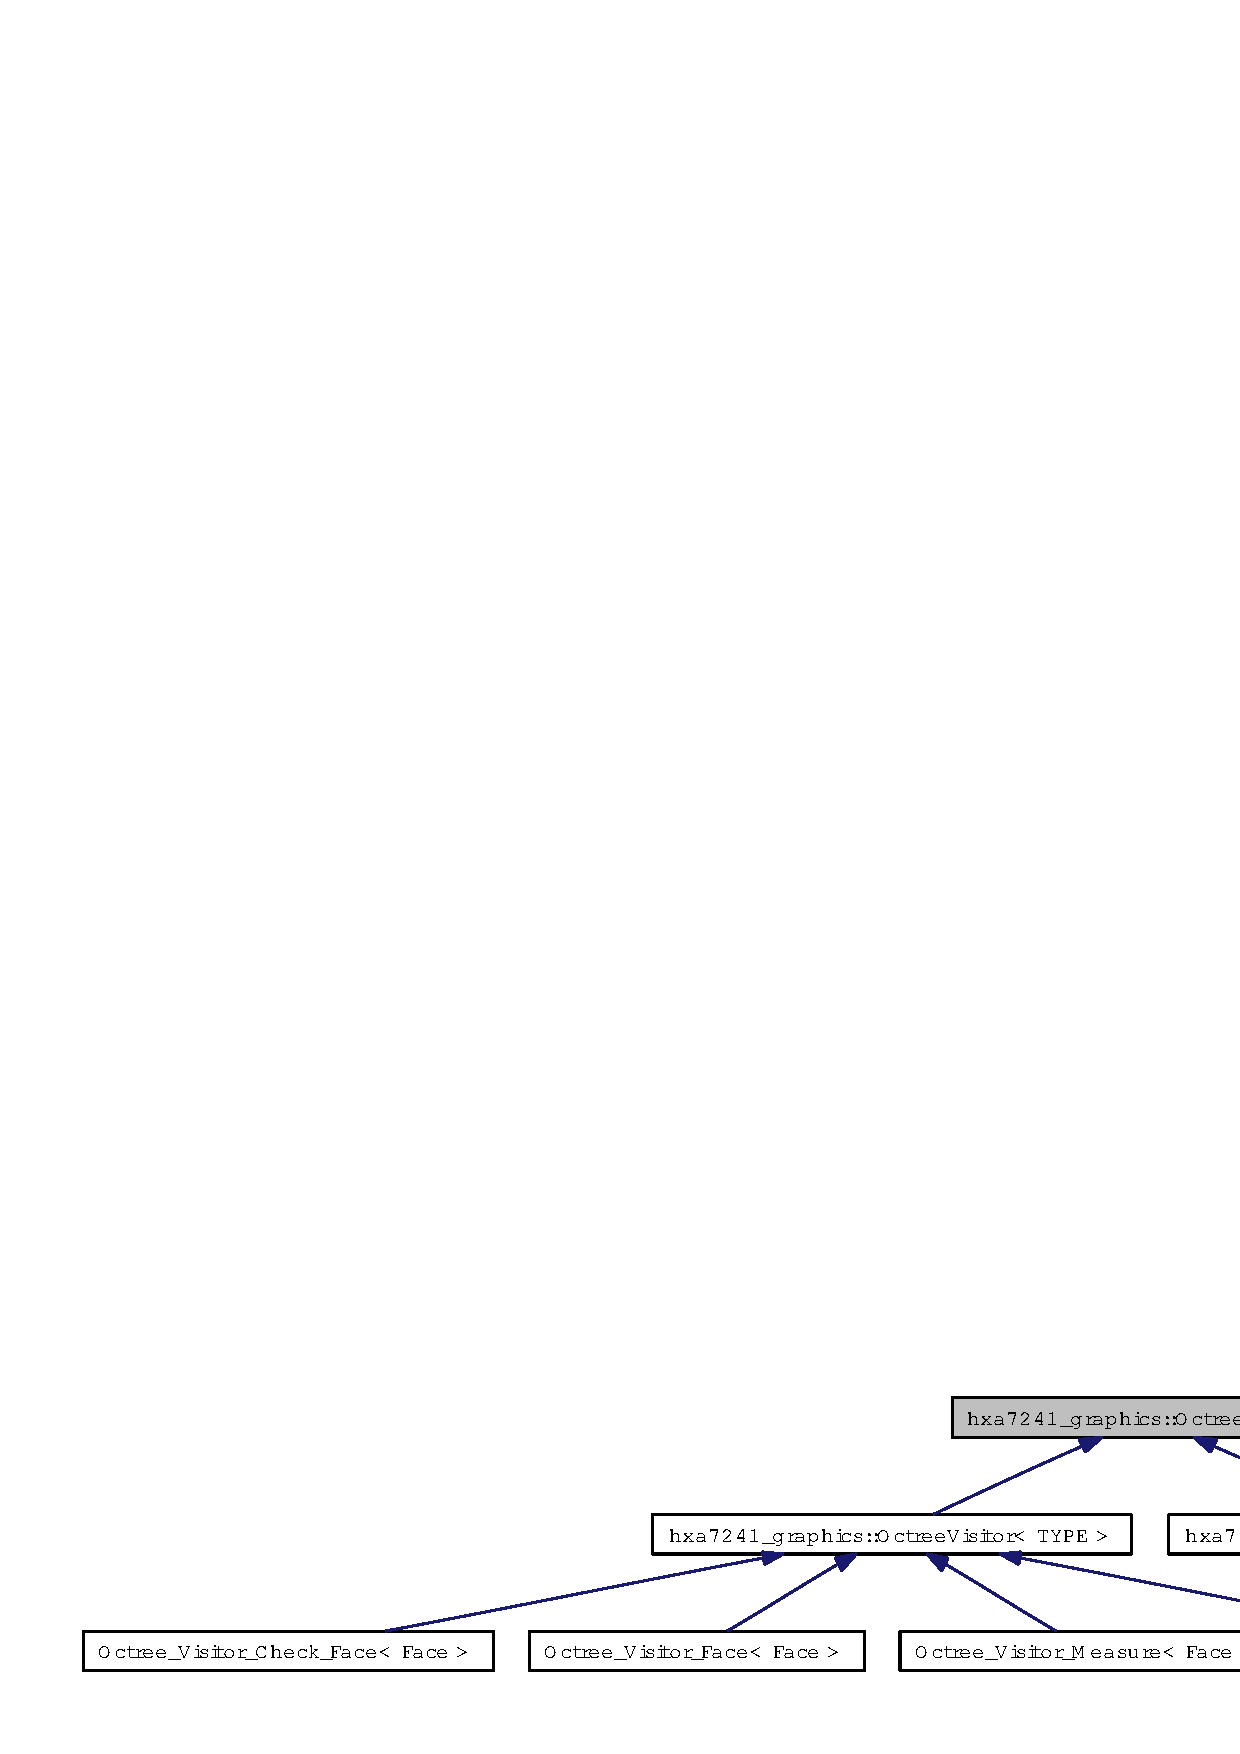
\includegraphics[width=404pt]{classhxa7241__graphics_1_1OctreeVisitorV__inherit__graph}
\end{center}
\end{figure}
\subsection*{Public Member Functions}
\begin{CompactItemize}
\item 
virtual {\bf $\sim$Octree\-Visitor\-V} ()
\item 
virtual void {\bf visit\-Root\-V} (const {\bf Octree\-Cell} $\ast$p\-Root\-Cell, const {\bf Octree\-Data} \&octree\-Data)=0
\begin{CompactList}\small\item\em commands ------------------------------------------------------------------- \item\end{CompactList}\item 
virtual void {\bf visit\-Branch\-V} (const {\bf Octree\-Cell} $\ast$sub\-Cells[8], const {\bf Octree\-Data} \&octree\-Data)=0
\item 
virtual void {\bf visit\-Leaf\-V} (const {\bf Array}$<$ const void $\ast$ $>$ \&items, const {\bf Octree\-Data} \&octree\-Data)=0
\end{CompactItemize}
\subsection*{Protected Member Functions}
\begin{CompactItemize}
\item 
{\bf Octree\-Visitor\-V} ()
\begin{CompactList}\small\item\em standard object services --------------------------------------------------- \item\end{CompactList}\end{CompactItemize}


\subsection{Detailed Description}
Visitor abstract base, for \doxyref{Octree}{p.}{classhxa7241__graphics_1_1Octree} implementation use.\par
\par


Subcell numbering: \small\begin{alltt}
    y z       6 7
    |/   2 3  4 5
     -x  0 1
 \end{alltt}
\normalsize 
 in binary: \small\begin{alltt}
    y z           110 111
    |/   010 011  100 101
     -x  000 001
 \end{alltt}
\normalsize 


\begin{Desc}
\item[See also:]\doxyref{Octree\-Cell}{p.}{classhxa7241__graphics_1_1OctreeCell} 

\doxyref{Octree\-Branch}{p.}{classhxa7241__graphics_1_1OctreeBranch} 

\doxyref{Octree\-Leaf}{p.}{classhxa7241__graphics_1_1OctreeLeaf} \end{Desc}




\subsection{Constructor \& Destructor Documentation}
\index{hxa7241_graphics::OctreeVisitorV@{hxa7241\_\-graphics::Octree\-Visitor\-V}!OctreeVisitorV@{OctreeVisitorV}}
\index{OctreeVisitorV@{OctreeVisitorV}!hxa7241_graphics::OctreeVisitorV@{hxa7241\_\-graphics::Octree\-Visitor\-V}}
\subsubsection{\setlength{\rightskip}{0pt plus 5cm}hxa7241\_\-graphics::Octree\-Visitor\-V::Octree\-Visitor\-V ()\hspace{0.3cm}{\tt  [inline, protected]}}\label{classhxa7241__graphics_1_1OctreeVisitorV_0df274bea5cf646cf00bddaeec28a25a}


standard object services --------------------------------------------------- 

\index{hxa7241_graphics::OctreeVisitorV@{hxa7241\_\-graphics::Octree\-Visitor\-V}!~OctreeVisitorV@{$\sim$OctreeVisitorV}}
\index{~OctreeVisitorV@{$\sim$OctreeVisitorV}!hxa7241_graphics::OctreeVisitorV@{hxa7241\_\-graphics::Octree\-Visitor\-V}}
\subsubsection{\setlength{\rightskip}{0pt plus 5cm}virtual hxa7241\_\-graphics::Octree\-Visitor\-V::$\sim$Octree\-Visitor\-V ()\hspace{0.3cm}{\tt  [inline, virtual]}}\label{classhxa7241__graphics_1_1OctreeVisitorV_bf944fed4ac9fe7fd190db50358db4ca}




\subsection{Member Function Documentation}
\index{hxa7241_graphics::OctreeVisitorV@{hxa7241\_\-graphics::Octree\-Visitor\-V}!visitRootV@{visitRootV}}
\index{visitRootV@{visitRootV}!hxa7241_graphics::OctreeVisitorV@{hxa7241\_\-graphics::Octree\-Visitor\-V}}
\subsubsection{\setlength{\rightskip}{0pt plus 5cm}virtual void hxa7241\_\-graphics::Octree\-Visitor\-V::visit\-Root\-V (const {\bf Octree\-Cell} $\ast$ {\em p\-Root\-Cell}, const {\bf Octree\-Data} \& {\em octree\-Data})\hspace{0.3cm}{\tt  [pure virtual]}}\label{classhxa7241__graphics_1_1OctreeVisitorV_ed002d0f93c17840c621f5840cf986e4}


commands ------------------------------------------------------------------- 



Implemented in {\bf hxa7241\_\-graphics::Octree\-Visitor$<$ TYPE $>$} \doxyref{}{p.}{classhxa7241__graphics_1_1OctreeVisitor_61cd041a87e104914494e99b5e9e7d8c}, and {\bf hxa7241\_\-graphics::Octree\-Visitor$<$ Face $>$} \doxyref{}{p.}{classhxa7241__graphics_1_1OctreeVisitor_61cd041a87e104914494e99b5e9e7d8c}.\index{hxa7241_graphics::OctreeVisitorV@{hxa7241\_\-graphics::Octree\-Visitor\-V}!visitBranchV@{visitBranchV}}
\index{visitBranchV@{visitBranchV}!hxa7241_graphics::OctreeVisitorV@{hxa7241\_\-graphics::Octree\-Visitor\-V}}
\subsubsection{\setlength{\rightskip}{0pt plus 5cm}virtual void hxa7241\_\-graphics::Octree\-Visitor\-V::visit\-Branch\-V (const {\bf Octree\-Cell} $\ast$ {\em sub\-Cells}[8], const {\bf Octree\-Data} \& {\em octree\-Data})\hspace{0.3cm}{\tt  [pure virtual]}}\label{classhxa7241__graphics_1_1OctreeVisitorV_69b3d1549ed26d237d9c515cc7ced0b4}




Implemented in {\bf hxa7241\_\-graphics::Octree\-Visitor$<$ TYPE $>$} \doxyref{}{p.}{classhxa7241__graphics_1_1OctreeVisitor_4e64e47d68d32ff6aac07bee49d8a84a}, and {\bf hxa7241\_\-graphics::Octree\-Visitor$<$ Face $>$} \doxyref{}{p.}{classhxa7241__graphics_1_1OctreeVisitor_4e64e47d68d32ff6aac07bee49d8a84a}.\index{hxa7241_graphics::OctreeVisitorV@{hxa7241\_\-graphics::Octree\-Visitor\-V}!visitLeafV@{visitLeafV}}
\index{visitLeafV@{visitLeafV}!hxa7241_graphics::OctreeVisitorV@{hxa7241\_\-graphics::Octree\-Visitor\-V}}
\subsubsection{\setlength{\rightskip}{0pt plus 5cm}virtual void hxa7241\_\-graphics::Octree\-Visitor\-V::visit\-Leaf\-V (const {\bf Array}$<$ const void $\ast$ $>$ \& {\em items}, const {\bf Octree\-Data} \& {\em octree\-Data})\hspace{0.3cm}{\tt  [pure virtual]}}\label{classhxa7241__graphics_1_1OctreeVisitorV_f805548bf0aca7122981d021a9846a9d}




Implemented in {\bf hxa7241\_\-graphics::Octree\-Visitor$<$ TYPE $>$} \doxyref{}{p.}{classhxa7241__graphics_1_1OctreeVisitor_bff12c6a7b9272b870d6c834ec92359c}, and {\bf hxa7241\_\-graphics::Octree\-Visitor$<$ Face $>$} \doxyref{}{p.}{classhxa7241__graphics_1_1OctreeVisitor_bff12c6a7b9272b870d6c834ec92359c}.

The documentation for this class was generated from the following file:\begin{CompactItemize}
\item 
{\bf Octree\-Auxiliary.h}\end{CompactItemize}

\section{Wm4::Quaternion$<$ Real $>$ Class Template Reference}
\label{classWm4_1_1Quaternion}\index{Wm4::Quaternion@{Wm4::Quaternion}}
{\tt \#include $<$Wm4Quaternion.h$>$}

Collaboration diagram for Wm4::Quaternion$<$ Real $>$:\begin{figure}[H]
\begin{center}
\leavevmode
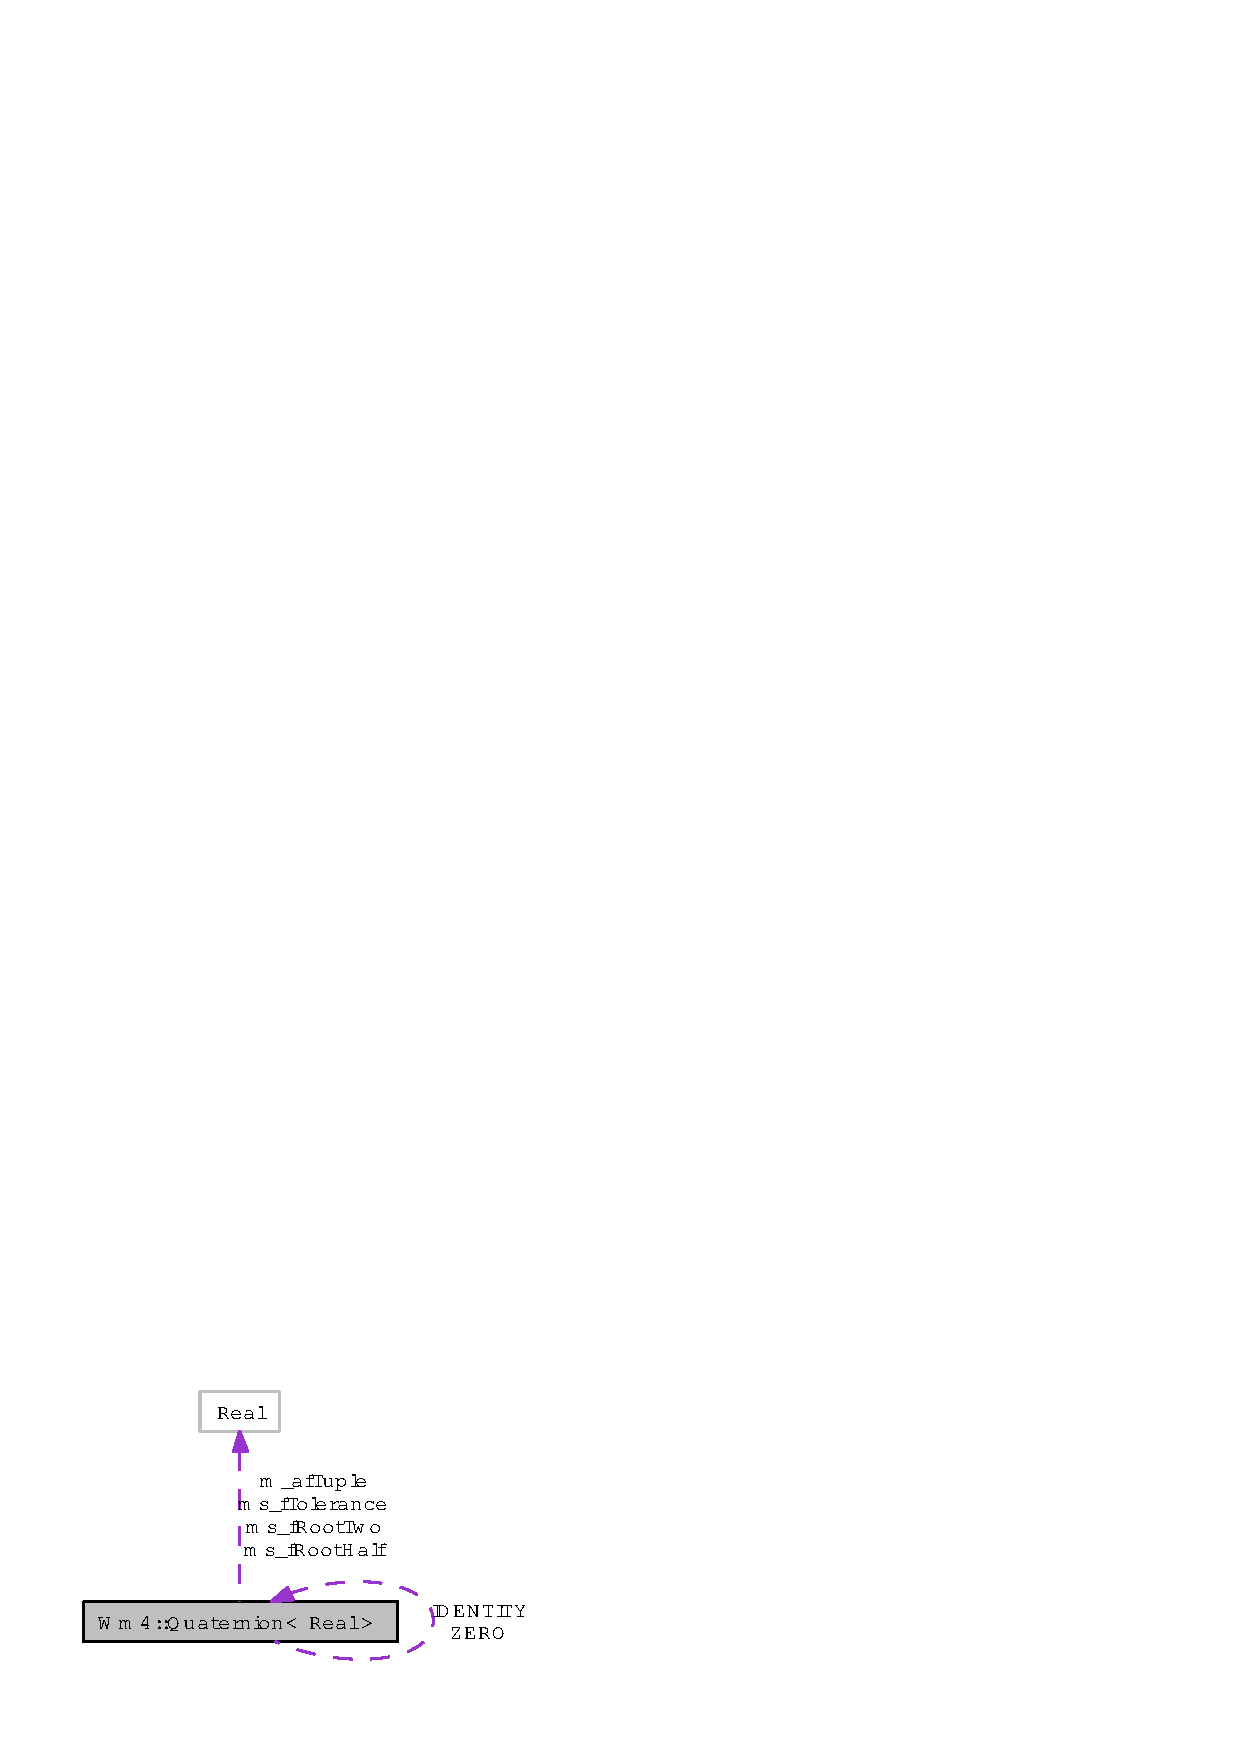
\includegraphics[width=129pt]{classWm4_1_1Quaternion__coll__graph}
\end{center}
\end{figure}
\subsection*{Public Member Functions}
\begin{CompactItemize}
\item 
{\bf Quaternion} ()
\item 
{\bf Quaternion} (Real f\-W, Real f\-X, Real f\-Y, Real f\-Z)
\item 
{\bf Quaternion} (const {\bf Quaternion} \&rk\-Q)
\item 
{\bf Quaternion} (const {\bf Matrix3}$<$ Real $>$ \&rk\-Rot)
\item 
{\bf Quaternion} (const {\bf Vector3}$<$ Real $>$ \&rk\-Axis, Real f\-Angle)
\item 
{\bf Quaternion} (const {\bf Vector3}$<$ Real $>$ ak\-Rot\-Column[3])
\item 
{\bf operator const Real $\ast$} () const
\item 
{\bf operator Real $\ast$} ()
\item 
Real {\bf operator[$\,$]} (int i) const
\item 
Real \& {\bf operator[$\,$]} (int i)
\item 
Real {\bf W} () const
\item 
Real \& {\bf W} ()
\item 
Real {\bf X} () const
\item 
Real \& {\bf X} ()
\item 
Real {\bf Y} () const
\item 
Real \& {\bf Y} ()
\item 
Real {\bf Z} () const
\item 
Real \& {\bf Z} ()
\item 
{\bf Quaternion} \& {\bf operator=} (const {\bf Quaternion} \&rk\-Q)
\item 
bool {\bf operator==} (const {\bf Quaternion} \&rk\-Q) const
\item 
bool {\bf operator!=} (const {\bf Quaternion} \&rk\-Q) const
\item 
bool {\bf operator$<$} (const {\bf Quaternion} \&rk\-Q) const
\item 
bool {\bf operator$<$=} (const {\bf Quaternion} \&rk\-Q) const
\item 
bool {\bf operator$>$} (const {\bf Quaternion} \&rk\-Q) const
\item 
bool {\bf operator$>$=} (const {\bf Quaternion} \&rk\-Q) const
\item 
{\bf Quaternion} {\bf operator+} (const {\bf Quaternion} \&rk\-Q) const
\item 
{\bf Quaternion} {\bf operator-} (const {\bf Quaternion} \&rk\-Q) const
\item 
{\bf Quaternion} {\bf operator $\ast$} (const {\bf Quaternion} \&rk\-Q) const
\item 
{\bf Quaternion} {\bf operator $\ast$} (Real f\-Scalar) const 
\item 
{\bf Quaternion} {\bf operator/} (Real f\-Scalar) const 
\item 
{\bf Quaternion} {\bf operator-} () const
\item 
{\bf Quaternion} \& {\bf operator+=} (const {\bf Quaternion} \&rk\-Q)
\item 
{\bf Quaternion} \& {\bf operator-=} (const {\bf Quaternion} \&rk\-Q)
\item 
{\bf Quaternion} \& {\bf operator $\ast$=} (Real f\-Scalar)
\item 
{\bf Quaternion} \& {\bf operator/=} (Real f\-Scalar)
\item 
{\bf Quaternion} \& {\bf From\-Rotation\-Matrix} (const {\bf Matrix3}$<$ Real $>$ \&rk\-Rot)
\item 
void {\bf To\-Rotation\-Matrix} ({\bf Matrix3}$<$ Real $>$ \&rk\-Rot) const
\item 
{\bf Quaternion} \& {\bf From\-Rotation\-Matrix} (const {\bf Vector3}$<$ Real $>$ ak\-Rot\-Column[3])
\item 
void {\bf To\-Rotation\-Matrix} ({\bf Vector3}$<$ Real $>$ ak\-Rot\-Column[3]) const
\item 
{\bf Quaternion} \& {\bf From\-Axis\-Angle} (const {\bf Vector3}$<$ Real $>$ \&rk\-Axis, Real f\-Angle)
\item 
void {\bf To\-Axis\-Angle} ({\bf Vector3}$<$ Real $>$ \&rk\-Axis, Real \&rf\-Angle) const
\item 
Real {\bf Length} () const
\item 
Real {\bf Squared\-Length} () const
\item 
Real {\bf Dot} (const {\bf Quaternion} \&rk\-Q) const
\item 
Real {\bf Normalize} ()
\item 
{\bf Quaternion} {\bf Inverse} () const
\item 
{\bf Quaternion} {\bf Conjugate} () const
\item 
{\bf Quaternion} {\bf Exp} () const
\item 
{\bf Quaternion} {\bf Log} () const
\item 
{\bf Vector3}$<$ Real $>$ {\bf Rotate} (const {\bf Vector3}$<$ Real $>$ \&rk\-Vector) const
\item 
{\bf Quaternion} \& {\bf Slerp} (Real f\-T, const {\bf Quaternion} \&rk\-P, const {\bf Quaternion} \&rk\-Q)
\item 
{\bf Quaternion} \& {\bf Slerp\-Extra\-Spins} (Real f\-T, const {\bf Quaternion} \&rk\-P, const {\bf Quaternion} \&rk\-Q, int i\-Extra\-Spins)
\item 
{\bf Quaternion} \& {\bf Intermediate} (const {\bf Quaternion} \&rk\-Q0, const {\bf Quaternion} \&rk\-Q1, const {\bf Quaternion} \&rk\-Q2)
\item 
{\bf Quaternion} \& {\bf Squad} (Real f\-T, const {\bf Quaternion} \&rk\-Q0, const {\bf Quaternion} \&rk\-A0, const {\bf Quaternion} \&rk\-A1, const {\bf Quaternion} \&rk\-Q1)
\item 
{\bf Quaternion} \& {\bf Align} (const {\bf Vector3}$<$ Real $>$ \&rk\-V1, const {\bf Vector3}$<$ Real $>$ \&rk\-V2)
\item 
void {\bf Decompose\-Twist\-Times\-Swing} (const {\bf Vector3}$<$ Real $>$ \&rk\-V1, {\bf Quaternion} \&rk\-Twist, {\bf Quaternion} \&rk\-Swing)
\item 
void {\bf Decompose\-Swing\-Times\-Twist} (const {\bf Vector3}$<$ Real $>$ \&rk\-V1, {\bf Quaternion} \&rk\-Swing, {\bf Quaternion} \&rk\-Twist)
\item 
{\bf Quaternion} {\bf Get\-Closest\-X} () const
\item 
{\bf Quaternion} {\bf Get\-Closest\-Y} () const
\item 
{\bf Quaternion} {\bf Get\-Closest\-Z} () const
\item 
{\bf Quaternion} {\bf Get\-Closest\-XY} () const
\item 
{\bf Quaternion} {\bf Get\-Closest\-YX} () const
\item 
{\bf Quaternion} {\bf Get\-Closest\-ZX} () const
\item 
{\bf Quaternion} {\bf Get\-Closest\-XZ} () const
\item 
{\bf Quaternion} {\bf Get\-Closest\-YZ} () const
\item 
{\bf Quaternion} {\bf Get\-Closest\-ZY} () const
\item 
void {\bf Factor\-XYZ} (Real \&rf\-Cx, Real \&rf\-Sx, Real \&rf\-Cy, Real \&rf\-Sy, Real \&rf\-Cz, Real \&rf\-Sz)
\item 
void {\bf Factor\-XZY} (Real \&rf\-Cx, Real \&rf\-Sx, Real \&rf\-Cz, Real \&rf\-Sz, Real \&rf\-Cy, Real \&rf\-Sy)
\item 
void {\bf Factor\-YZX} (Real \&rf\-Cy, Real \&rf\-Sy, Real \&rf\-Cz, Real \&rf\-Sz, Real \&rf\-Cx, Real \&rf\-Sx)
\item 
void {\bf Factor\-YXZ} (Real \&rf\-Cy, Real \&rf\-Sy, Real \&rf\-Cx, Real \&rf\-Sx, Real \&rf\-Cz, Real \&rf\-Sz)
\item 
void {\bf Factor\-ZXY} (Real \&rf\-Cz, Real \&rf\-Sz, Real \&rf\-Cx, Real \&rf\-Sx, Real \&rf\-Cy, Real \&rf\-Sy)
\item 
void {\bf Factor\-ZYX} (Real \&rf\-Cz, Real \&rf\-Sz, Real \&rf\-Cy, Real \&rf\-Sy, Real \&rf\-Cx, Real \&rf\-Sx)
\item 
{\bf Quaternion} {\bf Get\-Closest\-X} (const {\bf Constraints} \&rk\-XCon) const
\item 
{\bf Quaternion} {\bf Get\-Closest\-Y} (const {\bf Constraints} \&rk\-YCon) const
\item 
{\bf Quaternion} {\bf Get\-Closest\-Z} (const {\bf Constraints} \&rk\-ZCon) const
\item 
{\bf Quaternion} {\bf Get\-Closest\-XY} (const {\bf Constraints} \&rk\-XCon, const {\bf Constraints} \&rk\-YCon) const
\item 
{\bf Quaternion} {\bf Get\-Closest\-YX} (const {\bf Constraints} \&rk\-YCon, const {\bf Constraints} \&rk\-XCon) const
\item 
{\bf Quaternion} {\bf Get\-Closest\-ZX} (const {\bf Constraints} \&rk\-ZCon, const {\bf Constraints} \&rk\-XCon) const
\item 
{\bf Quaternion} {\bf Get\-Closest\-XZ} (const {\bf Constraints} \&rk\-XCon, const {\bf Constraints} \&rk\-ZCon) const
\item 
{\bf Quaternion} {\bf Get\-Closest\-ZY} (const {\bf Constraints} \&rk\-ZCon, const {\bf Constraints} \&rk\-YCon) const
\item 
{\bf Quaternion} {\bf Get\-Closest\-YZ} (const {\bf Constraints} \&rk\-YCon, const {\bf Constraints} \&rk\-ZCon) const
\item 
template$<$$>$ const {\bf Quaternion}$<$ float $>$ {\bf IDENTITY} (1.0f, 0.0f, 0.0f, 0.0f)
\item 
template$<$$>$ const {\bf Quaternion}$<$ float $>$ {\bf ZERO} (0.0f, 0.0f, 0.0f, 0.0f)
\item 
template$<$$>$ int {\bf ms\_\-i\-Next} [3]
\item 
template$<$$>$ float {\bf ms\_\-f\-Tolerance}
\item 
template$<$$>$ float {\bf ms\_\-f\-Root\-Two}
\item 
template$<$$>$ float {\bf ms\_\-f\-Root\-Half}
\item 
template$<$$>$ const {\bf Quaternion}$<$ double $>$ {\bf IDENTITY} (1.0, 0.0, 0.0, 0.0)
\item 
template$<$$>$ const {\bf Quaternion}$<$ double $>$ {\bf ZERO} (0.0, 0.0, 0.0, 0.0)
\item 
template$<$$>$ int {\bf ms\_\-i\-Next} [3]
\item 
template$<$$>$ double {\bf ms\_\-f\-Tolerance}
\item 
template$<$$>$ double {\bf ms\_\-f\-Root\-Two}
\item 
template$<$$>$ double {\bf ms\_\-f\-Root\-Half}
\end{CompactItemize}
\subsection*{Static Public Attributes}
\begin{CompactItemize}
\item 
static WM4\_\-FOUNDATION\_\-ITEM const {\bf Quaternion} {\bf IDENTITY}
\item 
static WM4\_\-FOUNDATION\_\-ITEM const {\bf Quaternion} {\bf ZERO}
\end{CompactItemize}
\subsection*{Classes}
\begin{CompactItemize}
\item 
class {\bf Constraints}
\end{CompactItemize}
\subsubsection*{template$<$class Real$>$ class Wm4::Quaternion$<$ Real $>$}



\subsection{Constructor \& Destructor Documentation}
\index{Wm4::Quaternion@{Wm4::Quaternion}!Quaternion@{Quaternion}}
\index{Quaternion@{Quaternion}!Wm4::Quaternion@{Wm4::Quaternion}}
\subsubsection{\setlength{\rightskip}{0pt plus 5cm}template$<$class Real$>$ {\bf Wm4::Quaternion}$<$ Real $>$::{\bf Quaternion} ()}\label{classWm4_1_1Quaternion_32466e45ed91a1f6aee0ab4024ebbfdf}


\index{Wm4::Quaternion@{Wm4::Quaternion}!Quaternion@{Quaternion}}
\index{Quaternion@{Quaternion}!Wm4::Quaternion@{Wm4::Quaternion}}
\subsubsection{\setlength{\rightskip}{0pt plus 5cm}template$<$class Real$>$ {\bf Wm4::Quaternion}$<$ Real $>$::{\bf Quaternion} (Real {\em f\-W}, Real {\em f\-X}, Real {\em f\-Y}, Real {\em f\-Z})}\label{classWm4_1_1Quaternion_4e41b6dc90db1e5bc27393944c1d419f}


\index{Wm4::Quaternion@{Wm4::Quaternion}!Quaternion@{Quaternion}}
\index{Quaternion@{Quaternion}!Wm4::Quaternion@{Wm4::Quaternion}}
\subsubsection{\setlength{\rightskip}{0pt plus 5cm}template$<$class Real$>$ {\bf Wm4::Quaternion}$<$ Real $>$::{\bf Quaternion} (const {\bf Quaternion}$<$ Real $>$ \& {\em rk\-Q})}\label{classWm4_1_1Quaternion_1a275cc89e8159c2ee75f01ac4000f55}


\index{Wm4::Quaternion@{Wm4::Quaternion}!Quaternion@{Quaternion}}
\index{Quaternion@{Quaternion}!Wm4::Quaternion@{Wm4::Quaternion}}
\subsubsection{\setlength{\rightskip}{0pt plus 5cm}template$<$class Real$>$ {\bf Wm4::Quaternion}$<$ Real $>$::{\bf Quaternion} (const {\bf Matrix3}$<$ Real $>$ \& {\em rk\-Rot})}\label{classWm4_1_1Quaternion_19dc773a1f4c008b2c9e090565bb6431}


\index{Wm4::Quaternion@{Wm4::Quaternion}!Quaternion@{Quaternion}}
\index{Quaternion@{Quaternion}!Wm4::Quaternion@{Wm4::Quaternion}}
\subsubsection{\setlength{\rightskip}{0pt plus 5cm}template$<$class Real$>$ {\bf Wm4::Quaternion}$<$ Real $>$::{\bf Quaternion} (const {\bf Vector3}$<$ Real $>$ \& {\em rk\-Axis}, Real {\em f\-Angle})}\label{classWm4_1_1Quaternion_0713966f31140f5169a0c3063c0b7430}


\index{Wm4::Quaternion@{Wm4::Quaternion}!Quaternion@{Quaternion}}
\index{Quaternion@{Quaternion}!Wm4::Quaternion@{Wm4::Quaternion}}
\subsubsection{\setlength{\rightskip}{0pt plus 5cm}template$<$class Real$>$ {\bf Wm4::Quaternion}$<$ Real $>$::{\bf Quaternion} (const {\bf Vector3}$<$ Real $>$ {\em ak\-Rot\-Column}[3])}\label{classWm4_1_1Quaternion_d3a3de3193121cf6adf22b7f3ba4428b}




\subsection{Member Function Documentation}
\index{Wm4::Quaternion@{Wm4::Quaternion}!operator const Real *@{operator const Real $\ast$}}
\index{operator const Real *@{operator const Real $\ast$}!Wm4::Quaternion@{Wm4::Quaternion}}
\subsubsection{\setlength{\rightskip}{0pt plus 5cm}template$<$class Real$>$ {\bf Wm4::Quaternion}$<$ Real $>$::operator const Real $\ast$ () const\hspace{0.3cm}{\tt  [inline]}}\label{classWm4_1_1Quaternion_2f86c976605cbaa01740720ce99a9342}


\index{Wm4::Quaternion@{Wm4::Quaternion}!operator Real *@{operator Real $\ast$}}
\index{operator Real *@{operator Real $\ast$}!Wm4::Quaternion@{Wm4::Quaternion}}
\subsubsection{\setlength{\rightskip}{0pt plus 5cm}template$<$class Real$>$ {\bf Wm4::Quaternion}$<$ Real $>$::operator Real $\ast$ ()\hspace{0.3cm}{\tt  [inline]}}\label{classWm4_1_1Quaternion_b4eaee550616a96095a0ab0a3ae1f028}


\index{Wm4::Quaternion@{Wm4::Quaternion}!operator[]@{operator[]}}
\index{operator[]@{operator[]}!Wm4::Quaternion@{Wm4::Quaternion}}
\subsubsection{\setlength{\rightskip}{0pt plus 5cm}template$<$class Real$>$ Real {\bf Wm4::Quaternion}$<$ Real $>$::operator[$\,$] (int {\em i}) const\hspace{0.3cm}{\tt  [inline]}}\label{classWm4_1_1Quaternion_e7561135811553160681730ca0d98670}


\index{Wm4::Quaternion@{Wm4::Quaternion}!operator[]@{operator[]}}
\index{operator[]@{operator[]}!Wm4::Quaternion@{Wm4::Quaternion}}
\subsubsection{\setlength{\rightskip}{0pt plus 5cm}template$<$class Real$>$ Real \& {\bf Wm4::Quaternion}$<$ Real $>$::operator[$\,$] (int {\em i})\hspace{0.3cm}{\tt  [inline]}}\label{classWm4_1_1Quaternion_50b4a53f03b7d8d84af62bcea70ed713}


\index{Wm4::Quaternion@{Wm4::Quaternion}!W@{W}}
\index{W@{W}!Wm4::Quaternion@{Wm4::Quaternion}}
\subsubsection{\setlength{\rightskip}{0pt plus 5cm}template$<$class Real$>$ Real {\bf Wm4::Quaternion}$<$ Real $>$::W () const\hspace{0.3cm}{\tt  [inline]}}\label{classWm4_1_1Quaternion_960f989a0ce9d6db3d9906c4d3ad5f1e}


\index{Wm4::Quaternion@{Wm4::Quaternion}!W@{W}}
\index{W@{W}!Wm4::Quaternion@{Wm4::Quaternion}}
\subsubsection{\setlength{\rightskip}{0pt plus 5cm}template$<$class Real$>$ Real \& {\bf Wm4::Quaternion}$<$ Real $>$::W ()\hspace{0.3cm}{\tt  [inline]}}\label{classWm4_1_1Quaternion_db69eb9cabe94f02734988a2e01a3484}


\index{Wm4::Quaternion@{Wm4::Quaternion}!X@{X}}
\index{X@{X}!Wm4::Quaternion@{Wm4::Quaternion}}
\subsubsection{\setlength{\rightskip}{0pt plus 5cm}template$<$class Real$>$ Real {\bf Wm4::Quaternion}$<$ Real $>$::X () const\hspace{0.3cm}{\tt  [inline]}}\label{classWm4_1_1Quaternion_bf365342d7c0e96d23673021f8e1087a}


\index{Wm4::Quaternion@{Wm4::Quaternion}!X@{X}}
\index{X@{X}!Wm4::Quaternion@{Wm4::Quaternion}}
\subsubsection{\setlength{\rightskip}{0pt plus 5cm}template$<$class Real$>$ Real \& {\bf Wm4::Quaternion}$<$ Real $>$::X ()\hspace{0.3cm}{\tt  [inline]}}\label{classWm4_1_1Quaternion_24b4aa16579caca3779d71ddcbd5e131}


\index{Wm4::Quaternion@{Wm4::Quaternion}!Y@{Y}}
\index{Y@{Y}!Wm4::Quaternion@{Wm4::Quaternion}}
\subsubsection{\setlength{\rightskip}{0pt plus 5cm}template$<$class Real$>$ Real {\bf Wm4::Quaternion}$<$ Real $>$::Y () const\hspace{0.3cm}{\tt  [inline]}}\label{classWm4_1_1Quaternion_d9ff560670b20d0f52270e0252fd95f2}


\index{Wm4::Quaternion@{Wm4::Quaternion}!Y@{Y}}
\index{Y@{Y}!Wm4::Quaternion@{Wm4::Quaternion}}
\subsubsection{\setlength{\rightskip}{0pt plus 5cm}template$<$class Real$>$ Real \& {\bf Wm4::Quaternion}$<$ Real $>$::Y ()\hspace{0.3cm}{\tt  [inline]}}\label{classWm4_1_1Quaternion_ab23f136c17695b188d4768ae9447b8a}


\index{Wm4::Quaternion@{Wm4::Quaternion}!Z@{Z}}
\index{Z@{Z}!Wm4::Quaternion@{Wm4::Quaternion}}
\subsubsection{\setlength{\rightskip}{0pt plus 5cm}template$<$class Real$>$ Real {\bf Wm4::Quaternion}$<$ Real $>$::Z () const\hspace{0.3cm}{\tt  [inline]}}\label{classWm4_1_1Quaternion_2438c994cabdd62a83b24753f0879f76}


\index{Wm4::Quaternion@{Wm4::Quaternion}!Z@{Z}}
\index{Z@{Z}!Wm4::Quaternion@{Wm4::Quaternion}}
\subsubsection{\setlength{\rightskip}{0pt plus 5cm}template$<$class Real$>$ Real \& {\bf Wm4::Quaternion}$<$ Real $>$::Z ()\hspace{0.3cm}{\tt  [inline]}}\label{classWm4_1_1Quaternion_7e47f1d93ceddf958af894a50213ac19}


\index{Wm4::Quaternion@{Wm4::Quaternion}!operator=@{operator=}}
\index{operator=@{operator=}!Wm4::Quaternion@{Wm4::Quaternion}}
\subsubsection{\setlength{\rightskip}{0pt plus 5cm}template$<$class Real$>$ {\bf Quaternion}$<$ Real $>$ \& {\bf Wm4::Quaternion}$<$ Real $>$::operator= (const {\bf Quaternion}$<$ Real $>$ \& {\em rk\-Q})\hspace{0.3cm}{\tt  [inline]}}\label{classWm4_1_1Quaternion_9f9051f46cc3b6e7c70d9cd0cd7f12ff}


\index{Wm4::Quaternion@{Wm4::Quaternion}!operator==@{operator==}}
\index{operator==@{operator==}!Wm4::Quaternion@{Wm4::Quaternion}}
\subsubsection{\setlength{\rightskip}{0pt plus 5cm}template$<$class Real$>$ bool {\bf Wm4::Quaternion}$<$ Real $>$::operator== (const {\bf Quaternion}$<$ Real $>$ \& {\em rk\-Q}) const}\label{classWm4_1_1Quaternion_17374f4682b525fbfc77bff020c6fa1f}


\index{Wm4::Quaternion@{Wm4::Quaternion}!operator"!=@{operator"!=}}
\index{operator"!=@{operator"!=}!Wm4::Quaternion@{Wm4::Quaternion}}
\subsubsection{\setlength{\rightskip}{0pt plus 5cm}template$<$class Real$>$ bool {\bf Wm4::Quaternion}$<$ Real $>$::operator!= (const {\bf Quaternion}$<$ Real $>$ \& {\em rk\-Q}) const}\label{classWm4_1_1Quaternion_8cfb7695938a7e9bc4595d17d95aebfd}


\index{Wm4::Quaternion@{Wm4::Quaternion}!operator<@{operator$<$}}
\index{operator<@{operator$<$}!Wm4::Quaternion@{Wm4::Quaternion}}
\subsubsection{\setlength{\rightskip}{0pt plus 5cm}template$<$class Real$>$ bool {\bf Wm4::Quaternion}$<$ Real $>$::operator$<$ (const {\bf Quaternion}$<$ Real $>$ \& {\em rk\-Q}) const}\label{classWm4_1_1Quaternion_8fc9a3f7f299e2f905946101e66d2d0d}


\index{Wm4::Quaternion@{Wm4::Quaternion}!operator<=@{operator$<$=}}
\index{operator<=@{operator$<$=}!Wm4::Quaternion@{Wm4::Quaternion}}
\subsubsection{\setlength{\rightskip}{0pt plus 5cm}template$<$class Real$>$ bool {\bf Wm4::Quaternion}$<$ Real $>$::operator$<$= (const {\bf Quaternion}$<$ Real $>$ \& {\em rk\-Q}) const}\label{classWm4_1_1Quaternion_9a96a03869dfd36baf811c0e44f67a34}


\index{Wm4::Quaternion@{Wm4::Quaternion}!operator>@{operator$>$}}
\index{operator>@{operator$>$}!Wm4::Quaternion@{Wm4::Quaternion}}
\subsubsection{\setlength{\rightskip}{0pt plus 5cm}template$<$class Real$>$ bool {\bf Wm4::Quaternion}$<$ Real $>$::operator$>$ (const {\bf Quaternion}$<$ Real $>$ \& {\em rk\-Q}) const}\label{classWm4_1_1Quaternion_d9e20bbdaca0df226c5eb293e28fb498}


\index{Wm4::Quaternion@{Wm4::Quaternion}!operator>=@{operator$>$=}}
\index{operator>=@{operator$>$=}!Wm4::Quaternion@{Wm4::Quaternion}}
\subsubsection{\setlength{\rightskip}{0pt plus 5cm}template$<$class Real$>$ bool {\bf Wm4::Quaternion}$<$ Real $>$::operator$>$= (const {\bf Quaternion}$<$ Real $>$ \& {\em rk\-Q}) const}\label{classWm4_1_1Quaternion_700a1803d1b5fa31db5aea71a40fa365}


\index{Wm4::Quaternion@{Wm4::Quaternion}!operator+@{operator+}}
\index{operator+@{operator+}!Wm4::Quaternion@{Wm4::Quaternion}}
\subsubsection{\setlength{\rightskip}{0pt plus 5cm}template$<$class Real$>$ {\bf Quaternion}$<$ Real $>$ {\bf Wm4::Quaternion}$<$ Real $>$::operator+ (const {\bf Quaternion}$<$ Real $>$ \& {\em rk\-Q}) const\hspace{0.3cm}{\tt  [inline]}}\label{classWm4_1_1Quaternion_853a41beda248fc365c7e4f27afeee2f}


\index{Wm4::Quaternion@{Wm4::Quaternion}!operator-@{operator-}}
\index{operator-@{operator-}!Wm4::Quaternion@{Wm4::Quaternion}}
\subsubsection{\setlength{\rightskip}{0pt plus 5cm}template$<$class Real$>$ {\bf Quaternion}$<$ Real $>$ {\bf Wm4::Quaternion}$<$ Real $>$::operator- (const {\bf Quaternion}$<$ Real $>$ \& {\em rk\-Q}) const\hspace{0.3cm}{\tt  [inline]}}\label{classWm4_1_1Quaternion_cd3975cac0be4c4399a2a7c5eab71ad9}


\index{Wm4::Quaternion@{Wm4::Quaternion}!operator *@{operator $\ast$}}
\index{operator *@{operator $\ast$}!Wm4::Quaternion@{Wm4::Quaternion}}
\subsubsection{\setlength{\rightskip}{0pt plus 5cm}template$<$class Real$>$ {\bf Quaternion}$<$ Real $>$ {\bf Wm4::Quaternion}$<$ Real $>$::operator $\ast$ (const {\bf Quaternion}$<$ Real $>$ \& {\em rk\-Q}) const\hspace{0.3cm}{\tt  [inline]}}\label{classWm4_1_1Quaternion_6bfd0d1486904570e2d5f8ab9c609714}


\index{Wm4::Quaternion@{Wm4::Quaternion}!operator *@{operator $\ast$}}
\index{operator *@{operator $\ast$}!Wm4::Quaternion@{Wm4::Quaternion}}
\subsubsection{\setlength{\rightskip}{0pt plus 5cm}template$<$class Real$>$ {\bf Quaternion}$<$ Real $>$ {\bf Wm4::Quaternion}$<$ Real $>$::operator $\ast$ (Real {\em f\-Scalar}) const\hspace{0.3cm}{\tt  [inline]}}\label{classWm4_1_1Quaternion_d42b7f0ebf0b164d3d6806078ffa5f6a}


\index{Wm4::Quaternion@{Wm4::Quaternion}!operator/@{operator/}}
\index{operator/@{operator/}!Wm4::Quaternion@{Wm4::Quaternion}}
\subsubsection{\setlength{\rightskip}{0pt plus 5cm}template$<$class Real$>$ {\bf Quaternion}$<$ Real $>$ {\bf Wm4::Quaternion}$<$ Real $>$::operator/ (Real {\em f\-Scalar}) const\hspace{0.3cm}{\tt  [inline]}}\label{classWm4_1_1Quaternion_07c3d0f906d7eda40d277380ca50b97f}


\index{Wm4::Quaternion@{Wm4::Quaternion}!operator-@{operator-}}
\index{operator-@{operator-}!Wm4::Quaternion@{Wm4::Quaternion}}
\subsubsection{\setlength{\rightskip}{0pt plus 5cm}template$<$class Real$>$ {\bf Quaternion}$<$ Real $>$ {\bf Wm4::Quaternion}$<$ Real $>$::operator- () const\hspace{0.3cm}{\tt  [inline]}}\label{classWm4_1_1Quaternion_9e92b601f1942231971eb3a84bd9649b}


\index{Wm4::Quaternion@{Wm4::Quaternion}!operator+=@{operator+=}}
\index{operator+=@{operator+=}!Wm4::Quaternion@{Wm4::Quaternion}}
\subsubsection{\setlength{\rightskip}{0pt plus 5cm}template$<$class Real$>$ {\bf Quaternion}$<$ Real $>$ \& {\bf Wm4::Quaternion}$<$ Real $>$::operator+= (const {\bf Quaternion}$<$ Real $>$ \& {\em rk\-Q})\hspace{0.3cm}{\tt  [inline]}}\label{classWm4_1_1Quaternion_b0ecdf716949ee56fd6b6f6fcf9ad2ca}


\index{Wm4::Quaternion@{Wm4::Quaternion}!operator-=@{operator-=}}
\index{operator-=@{operator-=}!Wm4::Quaternion@{Wm4::Quaternion}}
\subsubsection{\setlength{\rightskip}{0pt plus 5cm}template$<$class Real$>$ {\bf Quaternion}$<$ Real $>$ \& {\bf Wm4::Quaternion}$<$ Real $>$::operator-= (const {\bf Quaternion}$<$ Real $>$ \& {\em rk\-Q})\hspace{0.3cm}{\tt  [inline]}}\label{classWm4_1_1Quaternion_abc4c6eac448f8587a592b159485c872}


\index{Wm4::Quaternion@{Wm4::Quaternion}!operator *=@{operator $\ast$=}}
\index{operator *=@{operator $\ast$=}!Wm4::Quaternion@{Wm4::Quaternion}}
\subsubsection{\setlength{\rightskip}{0pt plus 5cm}template$<$class Real$>$ {\bf Quaternion}$<$ Real $>$ \& {\bf Wm4::Quaternion}$<$ Real $>$::operator $\ast$= (Real {\em f\-Scalar})\hspace{0.3cm}{\tt  [inline]}}\label{classWm4_1_1Quaternion_ac3d752a996ee6060b9bb624dd721195}


\index{Wm4::Quaternion@{Wm4::Quaternion}!operator/=@{operator/=}}
\index{operator/=@{operator/=}!Wm4::Quaternion@{Wm4::Quaternion}}
\subsubsection{\setlength{\rightskip}{0pt plus 5cm}template$<$class Real$>$ {\bf Quaternion}$<$ Real $>$ \& {\bf Wm4::Quaternion}$<$ Real $>$::operator/= (Real {\em f\-Scalar})\hspace{0.3cm}{\tt  [inline]}}\label{classWm4_1_1Quaternion_20d4f721888094693919d281601bac84}


\index{Wm4::Quaternion@{Wm4::Quaternion}!FromRotationMatrix@{FromRotationMatrix}}
\index{FromRotationMatrix@{FromRotationMatrix}!Wm4::Quaternion@{Wm4::Quaternion}}
\subsubsection{\setlength{\rightskip}{0pt plus 5cm}template$<$class Real$>$ {\bf Quaternion}$<$ Real $>$ \& {\bf Wm4::Quaternion}$<$ Real $>$::From\-Rotation\-Matrix (const {\bf Matrix3}$<$ Real $>$ \& {\em rk\-Rot})}\label{classWm4_1_1Quaternion_999ca8438ee2cc5d7bdb034a00054c8d}


\index{Wm4::Quaternion@{Wm4::Quaternion}!ToRotationMatrix@{ToRotationMatrix}}
\index{ToRotationMatrix@{ToRotationMatrix}!Wm4::Quaternion@{Wm4::Quaternion}}
\subsubsection{\setlength{\rightskip}{0pt plus 5cm}template$<$class Real$>$ void {\bf Wm4::Quaternion}$<$ Real $>$::To\-Rotation\-Matrix ({\bf Matrix3}$<$ Real $>$ \& {\em rk\-Rot}) const}\label{classWm4_1_1Quaternion_67ca867d76770511521bbc55eaeffb27}


\index{Wm4::Quaternion@{Wm4::Quaternion}!FromRotationMatrix@{FromRotationMatrix}}
\index{FromRotationMatrix@{FromRotationMatrix}!Wm4::Quaternion@{Wm4::Quaternion}}
\subsubsection{\setlength{\rightskip}{0pt plus 5cm}template$<$class Real$>$ {\bf Quaternion}$<$ Real $>$ \& {\bf Wm4::Quaternion}$<$ Real $>$::From\-Rotation\-Matrix (const {\bf Vector3}$<$ Real $>$ {\em ak\-Rot\-Column}[3])}\label{classWm4_1_1Quaternion_e111838a5863db8d32b939c64589f833}


\index{Wm4::Quaternion@{Wm4::Quaternion}!ToRotationMatrix@{ToRotationMatrix}}
\index{ToRotationMatrix@{ToRotationMatrix}!Wm4::Quaternion@{Wm4::Quaternion}}
\subsubsection{\setlength{\rightskip}{0pt plus 5cm}template$<$class Real$>$ void {\bf Wm4::Quaternion}$<$ Real $>$::To\-Rotation\-Matrix ({\bf Vector3}$<$ Real $>$ {\em ak\-Rot\-Column}[3]) const}\label{classWm4_1_1Quaternion_6eb3b7589399327cf2719f5a29789220}


\index{Wm4::Quaternion@{Wm4::Quaternion}!FromAxisAngle@{FromAxisAngle}}
\index{FromAxisAngle@{FromAxisAngle}!Wm4::Quaternion@{Wm4::Quaternion}}
\subsubsection{\setlength{\rightskip}{0pt plus 5cm}template$<$class Real$>$ {\bf Quaternion}$<$ Real $>$ \& {\bf Wm4::Quaternion}$<$ Real $>$::From\-Axis\-Angle (const {\bf Vector3}$<$ Real $>$ \& {\em rk\-Axis}, Real {\em f\-Angle})}\label{classWm4_1_1Quaternion_d097d07210266da3e52292151367f340}


\index{Wm4::Quaternion@{Wm4::Quaternion}!ToAxisAngle@{ToAxisAngle}}
\index{ToAxisAngle@{ToAxisAngle}!Wm4::Quaternion@{Wm4::Quaternion}}
\subsubsection{\setlength{\rightskip}{0pt plus 5cm}template$<$class Real$>$ void {\bf Wm4::Quaternion}$<$ Real $>$::To\-Axis\-Angle ({\bf Vector3}$<$ Real $>$ \& {\em rk\-Axis}, Real \& {\em rf\-Angle}) const}\label{classWm4_1_1Quaternion_25d66b10903a1f0a0c2cdcfcccc012dd}


\index{Wm4::Quaternion@{Wm4::Quaternion}!Length@{Length}}
\index{Length@{Length}!Wm4::Quaternion@{Wm4::Quaternion}}
\subsubsection{\setlength{\rightskip}{0pt plus 5cm}template$<$class Real$>$ Real {\bf Wm4::Quaternion}$<$ Real $>$::Length () const\hspace{0.3cm}{\tt  [inline]}}\label{classWm4_1_1Quaternion_f805700ec8fc3cee1c8daff3ecdfe88c}


\index{Wm4::Quaternion@{Wm4::Quaternion}!SquaredLength@{SquaredLength}}
\index{SquaredLength@{SquaredLength}!Wm4::Quaternion@{Wm4::Quaternion}}
\subsubsection{\setlength{\rightskip}{0pt plus 5cm}template$<$class Real$>$ Real {\bf Wm4::Quaternion}$<$ Real $>$::Squared\-Length () const\hspace{0.3cm}{\tt  [inline]}}\label{classWm4_1_1Quaternion_29e4ef607e51b0c034cdf0568c30f7cb}


\index{Wm4::Quaternion@{Wm4::Quaternion}!Dot@{Dot}}
\index{Dot@{Dot}!Wm4::Quaternion@{Wm4::Quaternion}}
\subsubsection{\setlength{\rightskip}{0pt plus 5cm}template$<$class Real$>$ Real {\bf Wm4::Quaternion}$<$ Real $>$::Dot (const {\bf Quaternion}$<$ Real $>$ \& {\em rk\-Q}) const\hspace{0.3cm}{\tt  [inline]}}\label{classWm4_1_1Quaternion_ea8c4800425d134db760bda44f5944bc}


\index{Wm4::Quaternion@{Wm4::Quaternion}!Normalize@{Normalize}}
\index{Normalize@{Normalize}!Wm4::Quaternion@{Wm4::Quaternion}}
\subsubsection{\setlength{\rightskip}{0pt plus 5cm}template$<$class Real$>$ Real {\bf Wm4::Quaternion}$<$ Real $>$::Normalize ()\hspace{0.3cm}{\tt  [inline]}}\label{classWm4_1_1Quaternion_b0df70264339a14241a2513883ece903}


\index{Wm4::Quaternion@{Wm4::Quaternion}!Inverse@{Inverse}}
\index{Inverse@{Inverse}!Wm4::Quaternion@{Wm4::Quaternion}}
\subsubsection{\setlength{\rightskip}{0pt plus 5cm}template$<$class Real$>$ {\bf Quaternion}$<$ Real $>$ {\bf Wm4::Quaternion}$<$ Real $>$::Inverse () const}\label{classWm4_1_1Quaternion_7adcfaa96c967518766a075832934f05}


\index{Wm4::Quaternion@{Wm4::Quaternion}!Conjugate@{Conjugate}}
\index{Conjugate@{Conjugate}!Wm4::Quaternion@{Wm4::Quaternion}}
\subsubsection{\setlength{\rightskip}{0pt plus 5cm}template$<$class Real$>$ {\bf Quaternion}$<$ Real $>$ {\bf Wm4::Quaternion}$<$ Real $>$::Conjugate () const}\label{classWm4_1_1Quaternion_ff8905d1a688dcbf07892de3be596b12}


\index{Wm4::Quaternion@{Wm4::Quaternion}!Exp@{Exp}}
\index{Exp@{Exp}!Wm4::Quaternion@{Wm4::Quaternion}}
\subsubsection{\setlength{\rightskip}{0pt plus 5cm}template$<$class Real$>$ {\bf Quaternion}$<$ Real $>$ {\bf Wm4::Quaternion}$<$ Real $>$::Exp () const}\label{classWm4_1_1Quaternion_fb4d38887cbd2c753ba7251c9447227a}


\index{Wm4::Quaternion@{Wm4::Quaternion}!Log@{Log}}
\index{Log@{Log}!Wm4::Quaternion@{Wm4::Quaternion}}
\subsubsection{\setlength{\rightskip}{0pt plus 5cm}template$<$class Real$>$ {\bf Quaternion}$<$ Real $>$ {\bf Wm4::Quaternion}$<$ Real $>$::{\bf Log} () const}\label{classWm4_1_1Quaternion_21a7fd3f85059e35d5edc10d1e8430d4}


\index{Wm4::Quaternion@{Wm4::Quaternion}!Rotate@{Rotate}}
\index{Rotate@{Rotate}!Wm4::Quaternion@{Wm4::Quaternion}}
\subsubsection{\setlength{\rightskip}{0pt plus 5cm}template$<$class Real$>$ {\bf Vector3}$<$ Real $>$ {\bf Wm4::Quaternion}$<$ Real $>$::Rotate (const {\bf Vector3}$<$ Real $>$ \& {\em rk\-Vector}) const}\label{classWm4_1_1Quaternion_f722d7183a96bea9115f77911c99bf70}


\index{Wm4::Quaternion@{Wm4::Quaternion}!Slerp@{Slerp}}
\index{Slerp@{Slerp}!Wm4::Quaternion@{Wm4::Quaternion}}
\subsubsection{\setlength{\rightskip}{0pt plus 5cm}template$<$class Real$>$ {\bf Quaternion}$<$ Real $>$ \& {\bf Wm4::Quaternion}$<$ Real $>$::Slerp (Real {\em f\-T}, const {\bf Quaternion}$<$ Real $>$ \& {\em rk\-P}, const {\bf Quaternion}$<$ Real $>$ \& {\em rk\-Q})}\label{classWm4_1_1Quaternion_0ec8407f839304a7e440ab290cf94c6c}


\index{Wm4::Quaternion@{Wm4::Quaternion}!SlerpExtraSpins@{SlerpExtraSpins}}
\index{SlerpExtraSpins@{SlerpExtraSpins}!Wm4::Quaternion@{Wm4::Quaternion}}
\subsubsection{\setlength{\rightskip}{0pt plus 5cm}template$<$class Real$>$ {\bf Quaternion}$<$ Real $>$ \& {\bf Wm4::Quaternion}$<$ Real $>$::Slerp\-Extra\-Spins (Real {\em f\-T}, const {\bf Quaternion}$<$ Real $>$ \& {\em rk\-P}, const {\bf Quaternion}$<$ Real $>$ \& {\em rk\-Q}, int {\em i\-Extra\-Spins})}\label{classWm4_1_1Quaternion_9a3d88bae1a77179140b32b03bd75fe2}


\index{Wm4::Quaternion@{Wm4::Quaternion}!Intermediate@{Intermediate}}
\index{Intermediate@{Intermediate}!Wm4::Quaternion@{Wm4::Quaternion}}
\subsubsection{\setlength{\rightskip}{0pt plus 5cm}template$<$class Real$>$ {\bf Quaternion}$<$ Real $>$ \& {\bf Wm4::Quaternion}$<$ Real $>$::Intermediate (const {\bf Quaternion}$<$ Real $>$ \& {\em rk\-Q0}, const {\bf Quaternion}$<$ Real $>$ \& {\em rk\-Q1}, const {\bf Quaternion}$<$ Real $>$ \& {\em rk\-Q2})}\label{classWm4_1_1Quaternion_78406c8173e77435e8ce1b13ef7c1f9c}


\index{Wm4::Quaternion@{Wm4::Quaternion}!Squad@{Squad}}
\index{Squad@{Squad}!Wm4::Quaternion@{Wm4::Quaternion}}
\subsubsection{\setlength{\rightskip}{0pt plus 5cm}template$<$class Real$>$ {\bf Quaternion}$<$ Real $>$ \& {\bf Wm4::Quaternion}$<$ Real $>$::Squad (Real {\em f\-T}, const {\bf Quaternion}$<$ Real $>$ \& {\em rk\-Q0}, const {\bf Quaternion}$<$ Real $>$ \& {\em rk\-A0}, const {\bf Quaternion}$<$ Real $>$ \& {\em rk\-A1}, const {\bf Quaternion}$<$ Real $>$ \& {\em rk\-Q1})}\label{classWm4_1_1Quaternion_b42ada6b188697a1d1bec34e78330ed0}


\index{Wm4::Quaternion@{Wm4::Quaternion}!Align@{Align}}
\index{Align@{Align}!Wm4::Quaternion@{Wm4::Quaternion}}
\subsubsection{\setlength{\rightskip}{0pt plus 5cm}template$<$class Real$>$ {\bf Quaternion}$<$ Real $>$ \& {\bf Wm4::Quaternion}$<$ Real $>$::Align (const {\bf Vector3}$<$ Real $>$ \& {\em rk\-V1}, const {\bf Vector3}$<$ Real $>$ \& {\em rk\-V2})}\label{classWm4_1_1Quaternion_afed22a39ac03d0b74984e133f1d1bed}


\index{Wm4::Quaternion@{Wm4::Quaternion}!DecomposeTwistTimesSwing@{DecomposeTwistTimesSwing}}
\index{DecomposeTwistTimesSwing@{DecomposeTwistTimesSwing}!Wm4::Quaternion@{Wm4::Quaternion}}
\subsubsection{\setlength{\rightskip}{0pt plus 5cm}template$<$class Real$>$ void {\bf Wm4::Quaternion}$<$ Real $>$::Decompose\-Twist\-Times\-Swing (const {\bf Vector3}$<$ Real $>$ \& {\em rk\-V1}, {\bf Quaternion}$<$ Real $>$ \& {\em rk\-Twist}, {\bf Quaternion}$<$ Real $>$ \& {\em rk\-Swing})}\label{classWm4_1_1Quaternion_70782459e82bba89d1f558db35989ede}


\index{Wm4::Quaternion@{Wm4::Quaternion}!DecomposeSwingTimesTwist@{DecomposeSwingTimesTwist}}
\index{DecomposeSwingTimesTwist@{DecomposeSwingTimesTwist}!Wm4::Quaternion@{Wm4::Quaternion}}
\subsubsection{\setlength{\rightskip}{0pt plus 5cm}template$<$class Real$>$ void {\bf Wm4::Quaternion}$<$ Real $>$::Decompose\-Swing\-Times\-Twist (const {\bf Vector3}$<$ Real $>$ \& {\em rk\-V1}, {\bf Quaternion}$<$ Real $>$ \& {\em rk\-Swing}, {\bf Quaternion}$<$ Real $>$ \& {\em rk\-Twist})}\label{classWm4_1_1Quaternion_9a117c3e9c8acbd6e7ae26a22bfdaf5c}


\index{Wm4::Quaternion@{Wm4::Quaternion}!GetClosestX@{GetClosestX}}
\index{GetClosestX@{GetClosestX}!Wm4::Quaternion@{Wm4::Quaternion}}
\subsubsection{\setlength{\rightskip}{0pt plus 5cm}template$<$class Real$>$ {\bf Quaternion}$<$ Real $>$ {\bf Wm4::Quaternion}$<$ Real $>$::Get\-Closest\-X () const}\label{classWm4_1_1Quaternion_d3e96bd350970366fcb2b0a09d984d10}


\index{Wm4::Quaternion@{Wm4::Quaternion}!GetClosestY@{GetClosestY}}
\index{GetClosestY@{GetClosestY}!Wm4::Quaternion@{Wm4::Quaternion}}
\subsubsection{\setlength{\rightskip}{0pt plus 5cm}template$<$class Real$>$ {\bf Quaternion}$<$ Real $>$ {\bf Wm4::Quaternion}$<$ Real $>$::Get\-Closest\-Y () const}\label{classWm4_1_1Quaternion_a2dd5d70dfd5f26a3024291474a6df66}


\index{Wm4::Quaternion@{Wm4::Quaternion}!GetClosestZ@{GetClosestZ}}
\index{GetClosestZ@{GetClosestZ}!Wm4::Quaternion@{Wm4::Quaternion}}
\subsubsection{\setlength{\rightskip}{0pt plus 5cm}template$<$class Real$>$ {\bf Quaternion}$<$ Real $>$ {\bf Wm4::Quaternion}$<$ Real $>$::Get\-Closest\-Z () const}\label{classWm4_1_1Quaternion_98ca51298f16fbb7223a9405b911970b}


\index{Wm4::Quaternion@{Wm4::Quaternion}!GetClosestXY@{GetClosestXY}}
\index{GetClosestXY@{GetClosestXY}!Wm4::Quaternion@{Wm4::Quaternion}}
\subsubsection{\setlength{\rightskip}{0pt plus 5cm}template$<$class Real$>$ {\bf Quaternion}$<$ Real $>$ {\bf Wm4::Quaternion}$<$ Real $>$::Get\-Closest\-XY () const}\label{classWm4_1_1Quaternion_e4b6087226aa6fc3ce6c7458b7d3bbbf}


\index{Wm4::Quaternion@{Wm4::Quaternion}!GetClosestYX@{GetClosestYX}}
\index{GetClosestYX@{GetClosestYX}!Wm4::Quaternion@{Wm4::Quaternion}}
\subsubsection{\setlength{\rightskip}{0pt plus 5cm}template$<$class Real$>$ {\bf Quaternion}$<$ Real $>$ {\bf Wm4::Quaternion}$<$ Real $>$::Get\-Closest\-YX () const}\label{classWm4_1_1Quaternion_910054a6b831f9965048e60b8706cf02}


\index{Wm4::Quaternion@{Wm4::Quaternion}!GetClosestZX@{GetClosestZX}}
\index{GetClosestZX@{GetClosestZX}!Wm4::Quaternion@{Wm4::Quaternion}}
\subsubsection{\setlength{\rightskip}{0pt plus 5cm}template$<$class Real$>$ {\bf Quaternion}$<$ Real $>$ {\bf Wm4::Quaternion}$<$ Real $>$::Get\-Closest\-ZX () const}\label{classWm4_1_1Quaternion_42ed27b9035d068f0c3bf8e3bfe88ae0}


\index{Wm4::Quaternion@{Wm4::Quaternion}!GetClosestXZ@{GetClosestXZ}}
\index{GetClosestXZ@{GetClosestXZ}!Wm4::Quaternion@{Wm4::Quaternion}}
\subsubsection{\setlength{\rightskip}{0pt plus 5cm}template$<$class Real$>$ {\bf Quaternion}$<$ Real $>$ {\bf Wm4::Quaternion}$<$ Real $>$::Get\-Closest\-XZ () const}\label{classWm4_1_1Quaternion_16a1d48db7c70e1c360f4ccd626043c2}


\index{Wm4::Quaternion@{Wm4::Quaternion}!GetClosestYZ@{GetClosestYZ}}
\index{GetClosestYZ@{GetClosestYZ}!Wm4::Quaternion@{Wm4::Quaternion}}
\subsubsection{\setlength{\rightskip}{0pt plus 5cm}template$<$class Real$>$ {\bf Quaternion}$<$ Real $>$ {\bf Wm4::Quaternion}$<$ Real $>$::Get\-Closest\-YZ () const}\label{classWm4_1_1Quaternion_2069a9806bb9cfddee4665a50d4e7997}


\index{Wm4::Quaternion@{Wm4::Quaternion}!GetClosestZY@{GetClosestZY}}
\index{GetClosestZY@{GetClosestZY}!Wm4::Quaternion@{Wm4::Quaternion}}
\subsubsection{\setlength{\rightskip}{0pt plus 5cm}template$<$class Real$>$ {\bf Quaternion}$<$ Real $>$ {\bf Wm4::Quaternion}$<$ Real $>$::Get\-Closest\-ZY () const}\label{classWm4_1_1Quaternion_ba055546010a994ca3556c74b6c22f27}


\index{Wm4::Quaternion@{Wm4::Quaternion}!FactorXYZ@{FactorXYZ}}
\index{FactorXYZ@{FactorXYZ}!Wm4::Quaternion@{Wm4::Quaternion}}
\subsubsection{\setlength{\rightskip}{0pt plus 5cm}template$<$class Real$>$ void {\bf Wm4::Quaternion}$<$ Real $>$::Factor\-XYZ (Real \& {\em rf\-Cx}, Real \& {\em rf\-Sx}, Real \& {\em rf\-Cy}, Real \& {\em rf\-Sy}, Real \& {\em rf\-Cz}, Real \& {\em rf\-Sz})}\label{classWm4_1_1Quaternion_420d3321c0d496f3f4a3b31ebd68f0d8}


\index{Wm4::Quaternion@{Wm4::Quaternion}!FactorXZY@{FactorXZY}}
\index{FactorXZY@{FactorXZY}!Wm4::Quaternion@{Wm4::Quaternion}}
\subsubsection{\setlength{\rightskip}{0pt plus 5cm}template$<$class Real$>$ void {\bf Wm4::Quaternion}$<$ Real $>$::Factor\-XZY (Real \& {\em rf\-Cx}, Real \& {\em rf\-Sx}, Real \& {\em rf\-Cz}, Real \& {\em rf\-Sz}, Real \& {\em rf\-Cy}, Real \& {\em rf\-Sy})}\label{classWm4_1_1Quaternion_1da1524e67dfadadd3d73796e124a741}


\index{Wm4::Quaternion@{Wm4::Quaternion}!FactorYZX@{FactorYZX}}
\index{FactorYZX@{FactorYZX}!Wm4::Quaternion@{Wm4::Quaternion}}
\subsubsection{\setlength{\rightskip}{0pt plus 5cm}template$<$class Real$>$ void {\bf Wm4::Quaternion}$<$ Real $>$::Factor\-YZX (Real \& {\em rf\-Cy}, Real \& {\em rf\-Sy}, Real \& {\em rf\-Cz}, Real \& {\em rf\-Sz}, Real \& {\em rf\-Cx}, Real \& {\em rf\-Sx})}\label{classWm4_1_1Quaternion_91edb7b79dc41cec01bd8c7cf6ba147f}


\index{Wm4::Quaternion@{Wm4::Quaternion}!FactorYXZ@{FactorYXZ}}
\index{FactorYXZ@{FactorYXZ}!Wm4::Quaternion@{Wm4::Quaternion}}
\subsubsection{\setlength{\rightskip}{0pt plus 5cm}template$<$class Real$>$ void {\bf Wm4::Quaternion}$<$ Real $>$::Factor\-YXZ (Real \& {\em rf\-Cy}, Real \& {\em rf\-Sy}, Real \& {\em rf\-Cx}, Real \& {\em rf\-Sx}, Real \& {\em rf\-Cz}, Real \& {\em rf\-Sz})}\label{classWm4_1_1Quaternion_4a3e790021f7eff98183820a6f573fc3}


\index{Wm4::Quaternion@{Wm4::Quaternion}!FactorZXY@{FactorZXY}}
\index{FactorZXY@{FactorZXY}!Wm4::Quaternion@{Wm4::Quaternion}}
\subsubsection{\setlength{\rightskip}{0pt plus 5cm}template$<$class Real$>$ void {\bf Wm4::Quaternion}$<$ Real $>$::Factor\-ZXY (Real \& {\em rf\-Cz}, Real \& {\em rf\-Sz}, Real \& {\em rf\-Cx}, Real \& {\em rf\-Sx}, Real \& {\em rf\-Cy}, Real \& {\em rf\-Sy})}\label{classWm4_1_1Quaternion_1624283bf14f6fab8c48e0d851de8d32}


\index{Wm4::Quaternion@{Wm4::Quaternion}!FactorZYX@{FactorZYX}}
\index{FactorZYX@{FactorZYX}!Wm4::Quaternion@{Wm4::Quaternion}}
\subsubsection{\setlength{\rightskip}{0pt plus 5cm}template$<$class Real$>$ void {\bf Wm4::Quaternion}$<$ Real $>$::Factor\-ZYX (Real \& {\em rf\-Cz}, Real \& {\em rf\-Sz}, Real \& {\em rf\-Cy}, Real \& {\em rf\-Sy}, Real \& {\em rf\-Cx}, Real \& {\em rf\-Sx})}\label{classWm4_1_1Quaternion_1b4c0d82c2f6873d5af2a98dcfa3064d}


\index{Wm4::Quaternion@{Wm4::Quaternion}!GetClosestX@{GetClosestX}}
\index{GetClosestX@{GetClosestX}!Wm4::Quaternion@{Wm4::Quaternion}}
\subsubsection{\setlength{\rightskip}{0pt plus 5cm}template$<$class Real$>$ {\bf Quaternion}$<$ Real $>$ {\bf Wm4::Quaternion}$<$ Real $>$::Get\-Closest\-X (const {\bf Constraints} \& {\em rk\-XCon}) const}\label{classWm4_1_1Quaternion_ceb69a5d390639469e085fc5a422d914}


\index{Wm4::Quaternion@{Wm4::Quaternion}!GetClosestY@{GetClosestY}}
\index{GetClosestY@{GetClosestY}!Wm4::Quaternion@{Wm4::Quaternion}}
\subsubsection{\setlength{\rightskip}{0pt plus 5cm}template$<$class Real$>$ {\bf Quaternion}$<$ Real $>$ {\bf Wm4::Quaternion}$<$ Real $>$::Get\-Closest\-Y (const {\bf Constraints} \& {\em rk\-YCon}) const}\label{classWm4_1_1Quaternion_834d0a6dd9494dd23e34cc6048257b4e}


\index{Wm4::Quaternion@{Wm4::Quaternion}!GetClosestZ@{GetClosestZ}}
\index{GetClosestZ@{GetClosestZ}!Wm4::Quaternion@{Wm4::Quaternion}}
\subsubsection{\setlength{\rightskip}{0pt plus 5cm}template$<$class Real$>$ {\bf Quaternion}$<$ Real $>$ {\bf Wm4::Quaternion}$<$ Real $>$::Get\-Closest\-Z (const {\bf Constraints} \& {\em rk\-ZCon}) const}\label{classWm4_1_1Quaternion_f5b0f63ffc089f0b62b4a5fe47e7f50e}


\index{Wm4::Quaternion@{Wm4::Quaternion}!GetClosestXY@{GetClosestXY}}
\index{GetClosestXY@{GetClosestXY}!Wm4::Quaternion@{Wm4::Quaternion}}
\subsubsection{\setlength{\rightskip}{0pt plus 5cm}template$<$class Real$>$ {\bf Quaternion}$<$ Real $>$ {\bf Wm4::Quaternion}$<$ Real $>$::Get\-Closest\-XY (const {\bf Constraints} \& {\em rk\-XCon}, const {\bf Constraints} \& {\em rk\-YCon}) const}\label{classWm4_1_1Quaternion_2c370f8a10467f94f68e444611b161ad}


\index{Wm4::Quaternion@{Wm4::Quaternion}!GetClosestYX@{GetClosestYX}}
\index{GetClosestYX@{GetClosestYX}!Wm4::Quaternion@{Wm4::Quaternion}}
\subsubsection{\setlength{\rightskip}{0pt plus 5cm}template$<$class Real$>$ {\bf Quaternion}$<$ Real $>$ {\bf Wm4::Quaternion}$<$ Real $>$::Get\-Closest\-YX (const {\bf Constraints} \& {\em rk\-YCon}, const {\bf Constraints} \& {\em rk\-XCon}) const}\label{classWm4_1_1Quaternion_abb2edebe0fd495fed9f2d8479cbf699}


\index{Wm4::Quaternion@{Wm4::Quaternion}!GetClosestZX@{GetClosestZX}}
\index{GetClosestZX@{GetClosestZX}!Wm4::Quaternion@{Wm4::Quaternion}}
\subsubsection{\setlength{\rightskip}{0pt plus 5cm}template$<$class Real$>$ {\bf Quaternion}$<$ Real $>$ {\bf Wm4::Quaternion}$<$ Real $>$::Get\-Closest\-ZX (const {\bf Constraints} \& {\em rk\-ZCon}, const {\bf Constraints} \& {\em rk\-XCon}) const}\label{classWm4_1_1Quaternion_a95edbc4adc16ef8879167e84fdfda7d}


\index{Wm4::Quaternion@{Wm4::Quaternion}!GetClosestXZ@{GetClosestXZ}}
\index{GetClosestXZ@{GetClosestXZ}!Wm4::Quaternion@{Wm4::Quaternion}}
\subsubsection{\setlength{\rightskip}{0pt plus 5cm}template$<$class Real$>$ {\bf Quaternion}$<$ Real $>$ {\bf Wm4::Quaternion}$<$ Real $>$::Get\-Closest\-XZ (const {\bf Constraints} \& {\em rk\-XCon}, const {\bf Constraints} \& {\em rk\-ZCon}) const}\label{classWm4_1_1Quaternion_b0424d935961db14096cec80ceb7c05d}


\index{Wm4::Quaternion@{Wm4::Quaternion}!GetClosestZY@{GetClosestZY}}
\index{GetClosestZY@{GetClosestZY}!Wm4::Quaternion@{Wm4::Quaternion}}
\subsubsection{\setlength{\rightskip}{0pt plus 5cm}template$<$class Real$>$ {\bf Quaternion}$<$ Real $>$ {\bf Wm4::Quaternion}$<$ Real $>$::Get\-Closest\-ZY (const {\bf Constraints} \& {\em rk\-ZCon}, const {\bf Constraints} \& {\em rk\-YCon}) const}\label{classWm4_1_1Quaternion_5beef9c556c27d8d981b5fc3fa9fdc34}


\index{Wm4::Quaternion@{Wm4::Quaternion}!GetClosestYZ@{GetClosestYZ}}
\index{GetClosestYZ@{GetClosestYZ}!Wm4::Quaternion@{Wm4::Quaternion}}
\subsubsection{\setlength{\rightskip}{0pt plus 5cm}template$<$class Real$>$ {\bf Quaternion}$<$ Real $>$ {\bf Wm4::Quaternion}$<$ Real $>$::Get\-Closest\-YZ (const {\bf Constraints} \& {\em rk\-YCon}, const {\bf Constraints} \& {\em rk\-ZCon}) const}\label{classWm4_1_1Quaternion_b9a245bad213a6ce5d8c35b2d4d48713}


\index{Wm4::Quaternion@{Wm4::Quaternion}!IDENTITY@{IDENTITY}}
\index{IDENTITY@{IDENTITY}!Wm4::Quaternion@{Wm4::Quaternion}}
\subsubsection{\setlength{\rightskip}{0pt plus 5cm}template$<$$>$ const {\bf Quaternion}$<$ float $>$ {\bf Wm4::Quaternion}$<$ float $>$::{\bf IDENTITY} (1. {\em 0f}, 0. {\em 0f}, 0. {\em 0f}, 0. {\em 0f})}\label{classWm4_1_1Quaternion_59288027790584fccd5c54d57a5589a2}


\index{Wm4::Quaternion@{Wm4::Quaternion}!ZERO@{ZERO}}
\index{ZERO@{ZERO}!Wm4::Quaternion@{Wm4::Quaternion}}
\subsubsection{\setlength{\rightskip}{0pt plus 5cm}template$<$$>$ const {\bf Quaternion}$<$ float $>$ {\bf Wm4::Quaternion}$<$ float $>$::{\bf ZERO} (0. {\em 0f}, 0. {\em 0f}, 0. {\em 0f}, 0. {\em 0f})}\label{classWm4_1_1Quaternion_ec90a2e0a977224b68532f33304de2f3}


\index{Wm4::Quaternion@{Wm4::Quaternion}!ms_iNext@{ms\_\-iNext}}
\index{ms_iNext@{ms\_\-iNext}!Wm4::Quaternion@{Wm4::Quaternion}}
\subsubsection{\setlength{\rightskip}{0pt plus 5cm}template$<$$>$ int {\bf Wm4::Quaternion}$<$ float $>$::ms\_\-i\-Next ()}\label{classWm4_1_1Quaternion_05174ba9862ca907a5185a11a7e2e389}


\index{Wm4::Quaternion@{Wm4::Quaternion}!ms_fTolerance@{ms\_\-fTolerance}}
\index{ms_fTolerance@{ms\_\-fTolerance}!Wm4::Quaternion@{Wm4::Quaternion}}
\subsubsection{\setlength{\rightskip}{0pt plus 5cm}template$<$$>$ float {\bf Wm4::Quaternion}$<$ float $>$::ms\_\-f\-Tolerance ()}\label{classWm4_1_1Quaternion_304f7d71a3b92582ce046bd540f0456a}


\index{Wm4::Quaternion@{Wm4::Quaternion}!ms_fRootTwo@{ms\_\-fRootTwo}}
\index{ms_fRootTwo@{ms\_\-fRootTwo}!Wm4::Quaternion@{Wm4::Quaternion}}
\subsubsection{\setlength{\rightskip}{0pt plus 5cm}template$<$$>$ float {\bf Wm4::Quaternion}$<$ float $>$::ms\_\-f\-Root\-Two ()}\label{classWm4_1_1Quaternion_76fd0e480dae5ecbfc91469cf0180019}


\index{Wm4::Quaternion@{Wm4::Quaternion}!ms_fRootHalf@{ms\_\-fRootHalf}}
\index{ms_fRootHalf@{ms\_\-fRootHalf}!Wm4::Quaternion@{Wm4::Quaternion}}
\subsubsection{\setlength{\rightskip}{0pt plus 5cm}template$<$$>$ float {\bf Wm4::Quaternion}$<$ float $>$::ms\_\-f\-Root\-Half ()}\label{classWm4_1_1Quaternion_a12eaa9511019cee51455f1fff46db9a}


\index{Wm4::Quaternion@{Wm4::Quaternion}!IDENTITY@{IDENTITY}}
\index{IDENTITY@{IDENTITY}!Wm4::Quaternion@{Wm4::Quaternion}}
\subsubsection{\setlength{\rightskip}{0pt plus 5cm}template$<$$>$ const {\bf Quaternion}$<$ double $>$ {\bf Wm4::Quaternion}$<$ double $>$::{\bf IDENTITY} (1. {\em 0}, 0. {\em 0}, 0. {\em 0}, 0. {\em 0})}\label{classWm4_1_1Quaternion_1a238f807517d926827e5c1b0e5ff29b}


\index{Wm4::Quaternion@{Wm4::Quaternion}!ZERO@{ZERO}}
\index{ZERO@{ZERO}!Wm4::Quaternion@{Wm4::Quaternion}}
\subsubsection{\setlength{\rightskip}{0pt plus 5cm}template$<$$>$ const {\bf Quaternion}$<$ double $>$ {\bf Wm4::Quaternion}$<$ double $>$::{\bf ZERO} (0. {\em 0}, 0. {\em 0}, 0. {\em 0}, 0. {\em 0})}\label{classWm4_1_1Quaternion_ab6454cbc8959189744465ed47ae90b0}


\index{Wm4::Quaternion@{Wm4::Quaternion}!ms_iNext@{ms\_\-iNext}}
\index{ms_iNext@{ms\_\-iNext}!Wm4::Quaternion@{Wm4::Quaternion}}
\subsubsection{\setlength{\rightskip}{0pt plus 5cm}template$<$$>$ int {\bf Wm4::Quaternion}$<$ double $>$::ms\_\-i\-Next ()}\label{classWm4_1_1Quaternion_bf4f129244f2ca051aaa91c3465f1f9d}


\index{Wm4::Quaternion@{Wm4::Quaternion}!ms_fTolerance@{ms\_\-fTolerance}}
\index{ms_fTolerance@{ms\_\-fTolerance}!Wm4::Quaternion@{Wm4::Quaternion}}
\subsubsection{\setlength{\rightskip}{0pt plus 5cm}template$<$$>$ double {\bf Wm4::Quaternion}$<$ double $>$::ms\_\-f\-Tolerance ()}\label{classWm4_1_1Quaternion_a9de22d187cdd57312c6f9d99a5f2f66}


\index{Wm4::Quaternion@{Wm4::Quaternion}!ms_fRootTwo@{ms\_\-fRootTwo}}
\index{ms_fRootTwo@{ms\_\-fRootTwo}!Wm4::Quaternion@{Wm4::Quaternion}}
\subsubsection{\setlength{\rightskip}{0pt plus 5cm}template$<$$>$ double {\bf Wm4::Quaternion}$<$ double $>$::ms\_\-f\-Root\-Two ()}\label{classWm4_1_1Quaternion_3b773db0e10149d2ca726ad44b072ee9}


\index{Wm4::Quaternion@{Wm4::Quaternion}!ms_fRootHalf@{ms\_\-fRootHalf}}
\index{ms_fRootHalf@{ms\_\-fRootHalf}!Wm4::Quaternion@{Wm4::Quaternion}}
\subsubsection{\setlength{\rightskip}{0pt plus 5cm}template$<$$>$ double {\bf Wm4::Quaternion}$<$ double $>$::ms\_\-f\-Root\-Half ()}\label{classWm4_1_1Quaternion_8699c62d3ca15c8bb09509a6efe87aaf}




\subsection{Member Data Documentation}
\index{Wm4::Quaternion@{Wm4::Quaternion}!IDENTITY@{IDENTITY}}
\index{IDENTITY@{IDENTITY}!Wm4::Quaternion@{Wm4::Quaternion}}
\subsubsection{\setlength{\rightskip}{0pt plus 5cm}template$<$class Real$>$ WM4\_\-FOUNDATION\_\-ITEM const {\bf Quaternion} {\bf Wm4::Quaternion}$<$ Real $>$::{\bf IDENTITY}\hspace{0.3cm}{\tt  [static]}}\label{classWm4_1_1Quaternion_0175525a86cac49cae5f80344d0e153e}


\index{Wm4::Quaternion@{Wm4::Quaternion}!ZERO@{ZERO}}
\index{ZERO@{ZERO}!Wm4::Quaternion@{Wm4::Quaternion}}
\subsubsection{\setlength{\rightskip}{0pt plus 5cm}template$<$class Real$>$ WM4\_\-FOUNDATION\_\-ITEM const {\bf Quaternion} {\bf Wm4::Quaternion}$<$ Real $>$::{\bf ZERO}\hspace{0.3cm}{\tt  [static]}}\label{classWm4_1_1Quaternion_ffff94f50a9f393355542f5ce16563f4}




The documentation for this class was generated from the following file:\begin{CompactItemize}
\item 
{\bf Wm4Quaternion.h}\end{CompactItemize}

\section{Wm4::Quaternion$<$ Real $>$::Constraints Class Reference}
\label{classWm4_1_1Quaternion_1_1Constraints}\index{Wm4::Quaternion::Constraints@{Wm4::Quaternion::Constraints}}
{\tt \#include $<$Wm4Quaternion.h$>$}

Collaboration diagram for Wm4::Quaternion$<$ Real $>$::Constraints:\begin{figure}[H]
\begin{center}
\leavevmode
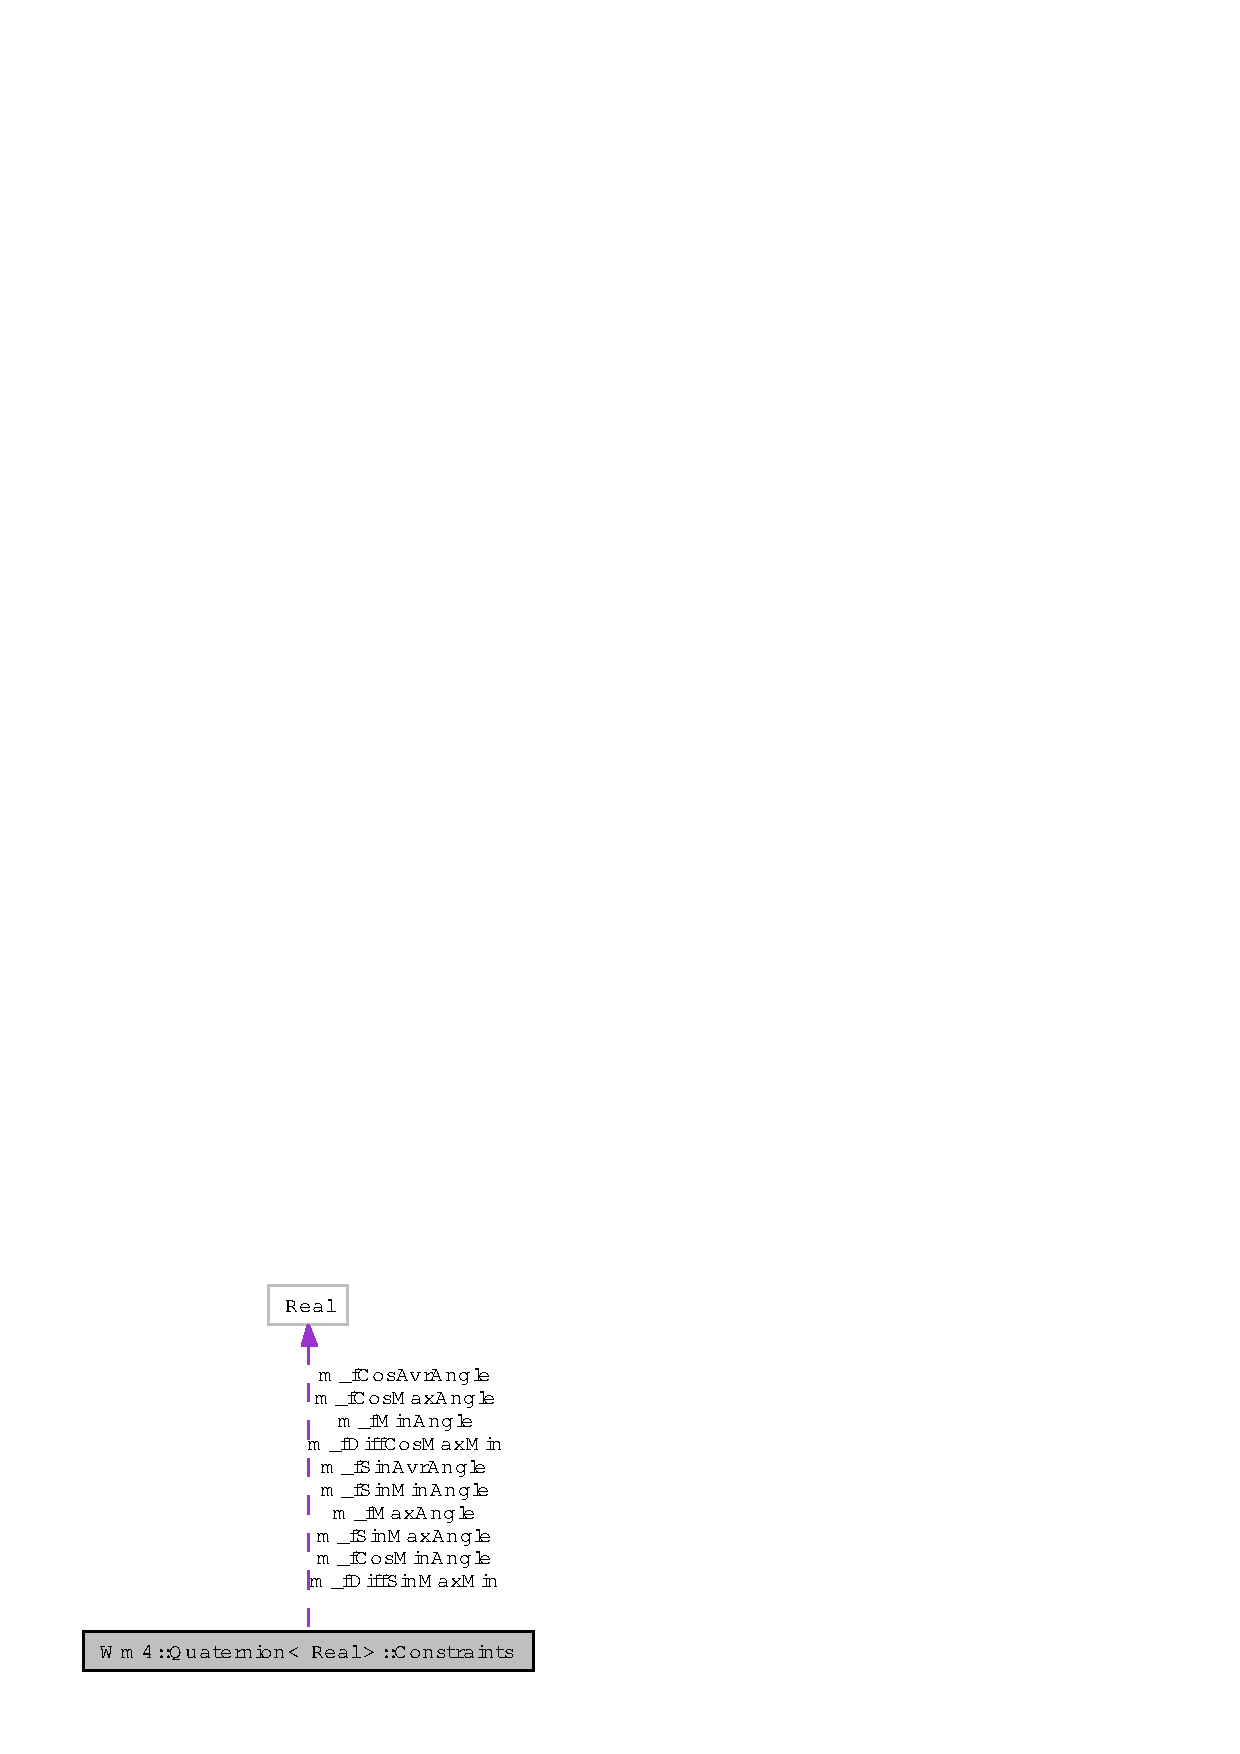
\includegraphics[width=130pt]{classWm4_1_1Quaternion_1_1Constraints__coll__graph}
\end{center}
\end{figure}
\subsection*{Public Member Functions}
\begin{CompactItemize}
\item 
{\bf Constraints} ()
\item 
{\bf Constraints} (Real f\-Min\-Angle, Real f\-Max\-Angle)
\item 
void {\bf Set\-Angles} (Real f\-Min\-Angle, Real f\-Max\-Angle)
\item 
bool {\bf Is\-Valid} (Real f\-X, Real f\-Y) const
\end{CompactItemize}
\subsection*{Public Attributes}
\begin{CompactItemize}
\item 
Real {\bf m\_\-f\-Min\-Angle}
\item 
Real {\bf m\_\-f\-Max\-Angle}
\item 
Real {\bf m\_\-f\-Cos\-Min\-Angle}
\item 
Real {\bf m\_\-f\-Sin\-Min\-Angle}
\item 
Real {\bf m\_\-f\-Cos\-Max\-Angle}
\item 
Real {\bf m\_\-f\-Sin\-Max\-Angle}
\item 
Real {\bf m\_\-f\-Diff\-Cos\-Max\-Min}
\item 
Real {\bf m\_\-f\-Diff\-Sin\-Max\-Min}
\item 
Real {\bf m\_\-f\-Cos\-Avr\-Angle}
\item 
Real {\bf m\_\-f\-Sin\-Avr\-Angle}
\end{CompactItemize}
\subsubsection*{template$<$class Real$>$ class Wm4::Quaternion$<$ Real $>$::Constraints}



\subsection{Constructor \& Destructor Documentation}
\index{Wm4::Quaternion::Constraints@{Wm4::Quaternion::Constraints}!Constraints@{Constraints}}
\index{Constraints@{Constraints}!Wm4::Quaternion::Constraints@{Wm4::Quaternion::Constraints}}
\subsubsection{\setlength{\rightskip}{0pt plus 5cm}template$<$class Real$>$ {\bf Wm4::Quaternion}$<$ Real $>$::Constraints::Constraints ()\hspace{0.3cm}{\tt  [inline]}}\label{classWm4_1_1Quaternion_1_1Constraints_baece2102271d37be19e4eb4250ae9a3}


\index{Wm4::Quaternion::Constraints@{Wm4::Quaternion::Constraints}!Constraints@{Constraints}}
\index{Constraints@{Constraints}!Wm4::Quaternion::Constraints@{Wm4::Quaternion::Constraints}}
\subsubsection{\setlength{\rightskip}{0pt plus 5cm}template$<$class Real$>$ {\bf Wm4::Quaternion}$<$ Real $>$::Constraints::Constraints (Real {\em f\-Min\-Angle}, Real {\em f\-Max\-Angle})\hspace{0.3cm}{\tt  [inline]}}\label{classWm4_1_1Quaternion_1_1Constraints_55ca3d50af6c74a9fccef44f2330e5ea}




\subsection{Member Function Documentation}
\index{Wm4::Quaternion::Constraints@{Wm4::Quaternion::Constraints}!SetAngles@{SetAngles}}
\index{SetAngles@{SetAngles}!Wm4::Quaternion::Constraints@{Wm4::Quaternion::Constraints}}
\subsubsection{\setlength{\rightskip}{0pt plus 5cm}template$<$class Real$>$ void {\bf Wm4::Quaternion}$<$ Real $>$::Constraints::Set\-Angles (Real {\em f\-Min\-Angle}, Real {\em f\-Max\-Angle})\hspace{0.3cm}{\tt  [inline]}}\label{classWm4_1_1Quaternion_1_1Constraints_6f960275d69caceaa6b59a8625ec1445}


\index{Wm4::Quaternion::Constraints@{Wm4::Quaternion::Constraints}!IsValid@{IsValid}}
\index{IsValid@{IsValid}!Wm4::Quaternion::Constraints@{Wm4::Quaternion::Constraints}}
\subsubsection{\setlength{\rightskip}{0pt plus 5cm}template$<$class Real$>$ bool {\bf Wm4::Quaternion}$<$ Real $>$::Constraints::Is\-Valid (Real {\em f\-X}, Real {\em f\-Y}) const\hspace{0.3cm}{\tt  [inline]}}\label{classWm4_1_1Quaternion_1_1Constraints_5b65cbee15c31fa6159b780cc7f3d17b}




\subsection{Member Data Documentation}
\index{Wm4::Quaternion::Constraints@{Wm4::Quaternion::Constraints}!m_fMinAngle@{m\_\-fMinAngle}}
\index{m_fMinAngle@{m\_\-fMinAngle}!Wm4::Quaternion::Constraints@{Wm4::Quaternion::Constraints}}
\subsubsection{\setlength{\rightskip}{0pt plus 5cm}template$<$class Real$>$ Real {\bf Wm4::Quaternion}$<$ Real $>$::{\bf Constraints::m\_\-f\-Min\-Angle}}\label{classWm4_1_1Quaternion_1_1Constraints_0ca98fffa124a20b421841c4eb423da2}


\index{Wm4::Quaternion::Constraints@{Wm4::Quaternion::Constraints}!m_fMaxAngle@{m\_\-fMaxAngle}}
\index{m_fMaxAngle@{m\_\-fMaxAngle}!Wm4::Quaternion::Constraints@{Wm4::Quaternion::Constraints}}
\subsubsection{\setlength{\rightskip}{0pt plus 5cm}template$<$class Real$>$ Real {\bf Wm4::Quaternion}$<$ Real $>$::{\bf Constraints::m\_\-f\-Max\-Angle}}\label{classWm4_1_1Quaternion_1_1Constraints_e6ce1299891268fb1436e638ac132df6}


\index{Wm4::Quaternion::Constraints@{Wm4::Quaternion::Constraints}!m_fCosMinAngle@{m\_\-fCosMinAngle}}
\index{m_fCosMinAngle@{m\_\-fCosMinAngle}!Wm4::Quaternion::Constraints@{Wm4::Quaternion::Constraints}}
\subsubsection{\setlength{\rightskip}{0pt plus 5cm}template$<$class Real$>$ Real {\bf Wm4::Quaternion}$<$ Real $>$::{\bf Constraints::m\_\-f\-Cos\-Min\-Angle}}\label{classWm4_1_1Quaternion_1_1Constraints_200176cd38eb222bca852af2760a26cb}


\index{Wm4::Quaternion::Constraints@{Wm4::Quaternion::Constraints}!m_fSinMinAngle@{m\_\-fSinMinAngle}}
\index{m_fSinMinAngle@{m\_\-fSinMinAngle}!Wm4::Quaternion::Constraints@{Wm4::Quaternion::Constraints}}
\subsubsection{\setlength{\rightskip}{0pt plus 5cm}template$<$class Real$>$ Real {\bf Wm4::Quaternion}$<$ Real $>$::{\bf Constraints::m\_\-f\-Sin\-Min\-Angle}}\label{classWm4_1_1Quaternion_1_1Constraints_d75bd2fdbb8a3bab1dc095f22ff040da}


\index{Wm4::Quaternion::Constraints@{Wm4::Quaternion::Constraints}!m_fCosMaxAngle@{m\_\-fCosMaxAngle}}
\index{m_fCosMaxAngle@{m\_\-fCosMaxAngle}!Wm4::Quaternion::Constraints@{Wm4::Quaternion::Constraints}}
\subsubsection{\setlength{\rightskip}{0pt plus 5cm}template$<$class Real$>$ Real {\bf Wm4::Quaternion}$<$ Real $>$::{\bf Constraints::m\_\-f\-Cos\-Max\-Angle}}\label{classWm4_1_1Quaternion_1_1Constraints_631f472b174a215e84582144b0b37856}


\index{Wm4::Quaternion::Constraints@{Wm4::Quaternion::Constraints}!m_fSinMaxAngle@{m\_\-fSinMaxAngle}}
\index{m_fSinMaxAngle@{m\_\-fSinMaxAngle}!Wm4::Quaternion::Constraints@{Wm4::Quaternion::Constraints}}
\subsubsection{\setlength{\rightskip}{0pt plus 5cm}template$<$class Real$>$ Real {\bf Wm4::Quaternion}$<$ Real $>$::{\bf Constraints::m\_\-f\-Sin\-Max\-Angle}}\label{classWm4_1_1Quaternion_1_1Constraints_f36569255d026380f058ab889389885b}


\index{Wm4::Quaternion::Constraints@{Wm4::Quaternion::Constraints}!m_fDiffCosMaxMin@{m\_\-fDiffCosMaxMin}}
\index{m_fDiffCosMaxMin@{m\_\-fDiffCosMaxMin}!Wm4::Quaternion::Constraints@{Wm4::Quaternion::Constraints}}
\subsubsection{\setlength{\rightskip}{0pt plus 5cm}template$<$class Real$>$ Real {\bf Wm4::Quaternion}$<$ Real $>$::{\bf Constraints::m\_\-f\-Diff\-Cos\-Max\-Min}}\label{classWm4_1_1Quaternion_1_1Constraints_d514455d5bb32591c0efdbb4f124c3b0}


\index{Wm4::Quaternion::Constraints@{Wm4::Quaternion::Constraints}!m_fDiffSinMaxMin@{m\_\-fDiffSinMaxMin}}
\index{m_fDiffSinMaxMin@{m\_\-fDiffSinMaxMin}!Wm4::Quaternion::Constraints@{Wm4::Quaternion::Constraints}}
\subsubsection{\setlength{\rightskip}{0pt plus 5cm}template$<$class Real$>$ Real {\bf Wm4::Quaternion}$<$ Real $>$::{\bf Constraints::m\_\-f\-Diff\-Sin\-Max\-Min}}\label{classWm4_1_1Quaternion_1_1Constraints_daeefc19ed556605868b2c15ae4bddb9}


\index{Wm4::Quaternion::Constraints@{Wm4::Quaternion::Constraints}!m_fCosAvrAngle@{m\_\-fCosAvrAngle}}
\index{m_fCosAvrAngle@{m\_\-fCosAvrAngle}!Wm4::Quaternion::Constraints@{Wm4::Quaternion::Constraints}}
\subsubsection{\setlength{\rightskip}{0pt plus 5cm}template$<$class Real$>$ Real {\bf Wm4::Quaternion}$<$ Real $>$::{\bf Constraints::m\_\-f\-Cos\-Avr\-Angle}}\label{classWm4_1_1Quaternion_1_1Constraints_91d840dba1dbee1313e4ecd6b1e450bb}


\index{Wm4::Quaternion::Constraints@{Wm4::Quaternion::Constraints}!m_fSinAvrAngle@{m\_\-fSinAvrAngle}}
\index{m_fSinAvrAngle@{m\_\-fSinAvrAngle}!Wm4::Quaternion::Constraints@{Wm4::Quaternion::Constraints}}
\subsubsection{\setlength{\rightskip}{0pt plus 5cm}template$<$class Real$>$ Real {\bf Wm4::Quaternion}$<$ Real $>$::{\bf Constraints::m\_\-f\-Sin\-Avr\-Angle}}\label{classWm4_1_1Quaternion_1_1Constraints_57d21a9c2f9c4609df3a702194ebffe5}




The documentation for this class was generated from the following file:\begin{CompactItemize}
\item 
{\bf Wm4Quaternion.h}\end{CompactItemize}

\section{Refractory Class Reference}
\label{classRefractory}\index{Refractory@{Refractory}}
{\tt \#include $<$refractory.h$>$}

Collaboration diagram for Refractory:\begin{figure}[H]
\begin{center}
\leavevmode
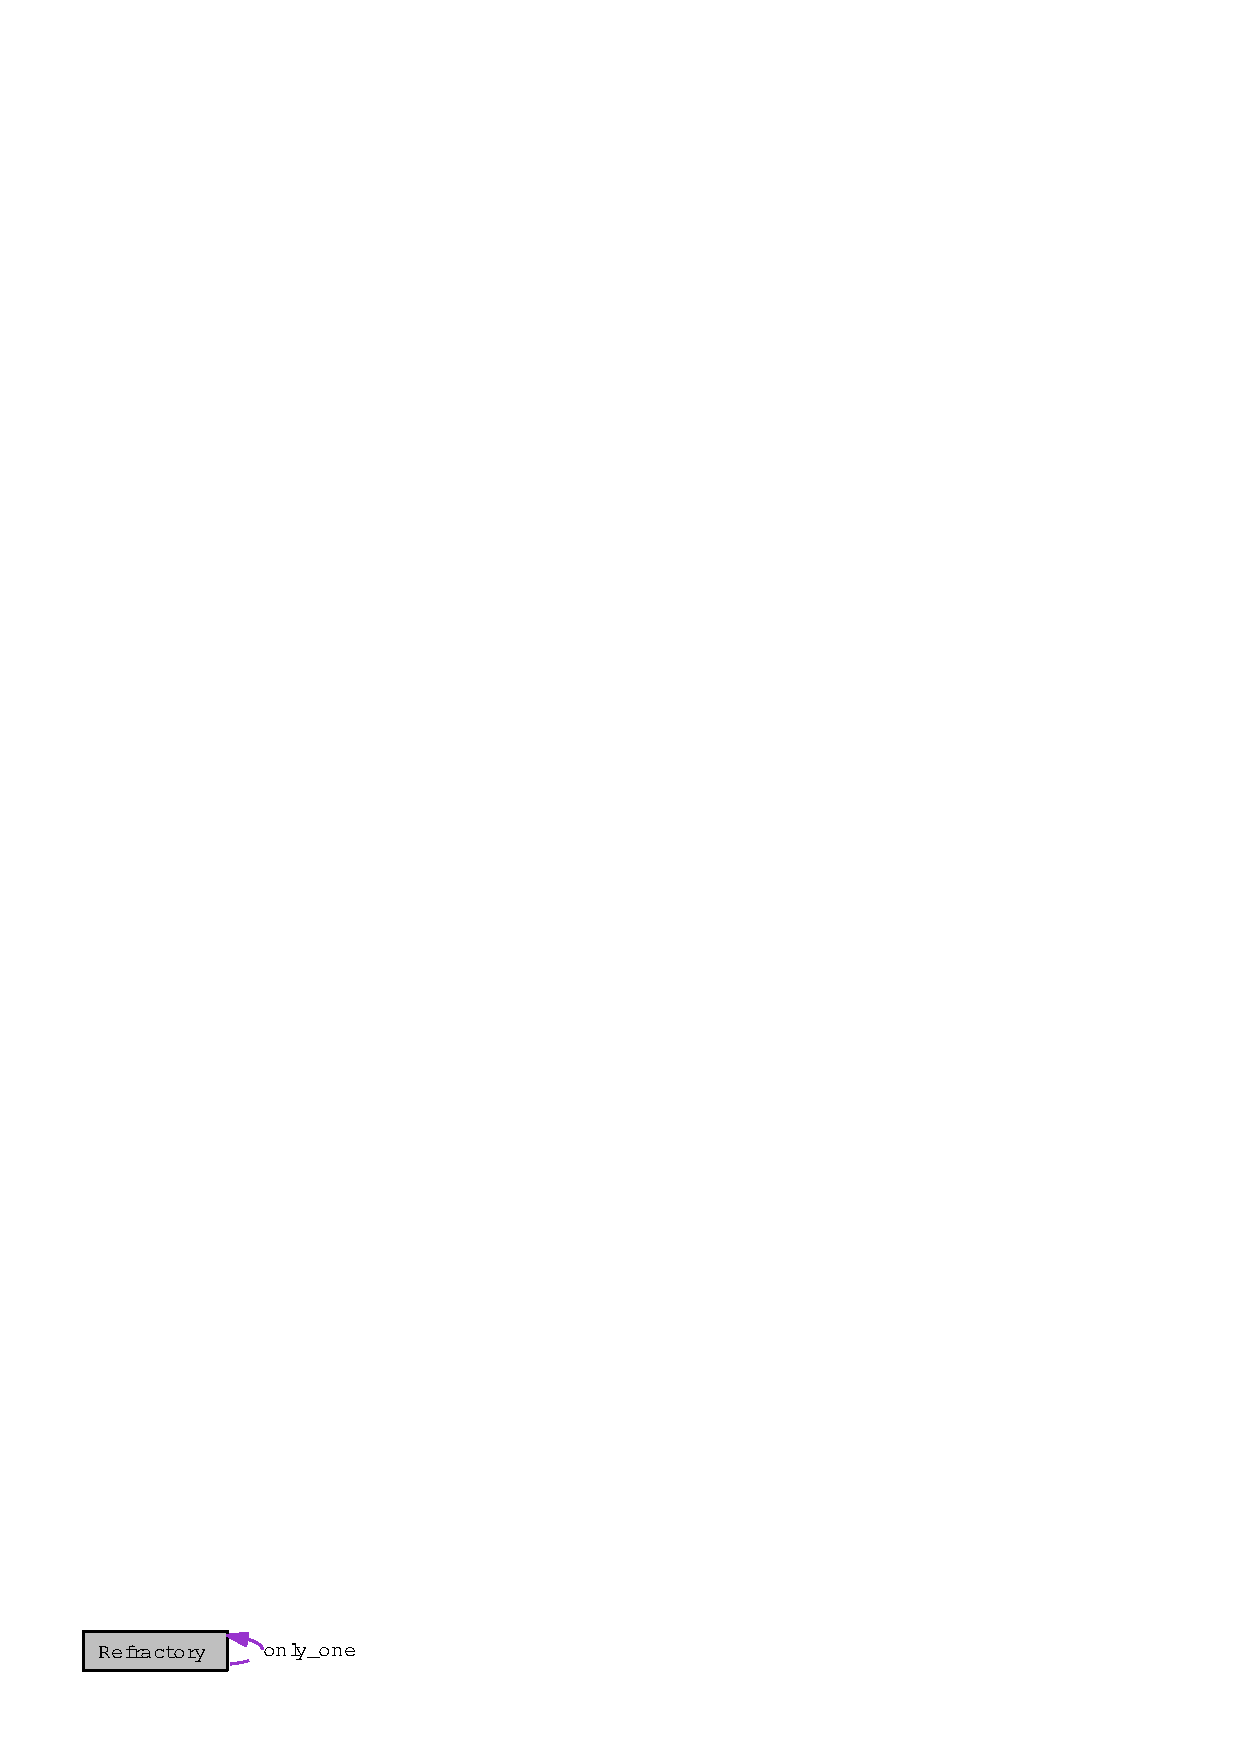
\includegraphics[width=88pt]{classRefractory__coll__graph}
\end{center}
\end{figure}
\subsection*{Public Member Functions}
\begin{CompactItemize}
\item 
int {\bf num\-Recorded\-Vertex\-Moves} ({\bf Vertex} $\ast$)
\item 
int {\bf get\-Num\-Vert\-Refracted\-N} (void) const
\item 
int {\bf get\-Num\-Vert\-Refracted\-Int} (void) const
\item 
int {\bf get\-Num\-Vert\-Refracted\-Ang} (void) const
\item 
int {\bf get\-Num\-Vert\-Refracted\-Small\-Disp} (void) const
\item 
int {\bf get\-Num\-Vert\-Refracted\-Octree\-Vio} (void) const
\item 
bool {\bf is\-Refracted} ({\bf Vertex} $\ast$const)
\item 
bool {\bf vertex\-Is\-Move\-Candidate} ({\bf Vertex} $\ast$const v)
\item 
bool {\bf vertex\-Moves\-Are\-Recorded} ({\bf Vertex} $\ast$)
\item 
void {\bf refract\-Vertex\-For\-Small\-Disp\-Vio} ({\bf Vertex} $\ast$const)
\item 
void {\bf refract\-Vertex\-For\-Int\-Vio} ({\bf Vertex} $\ast$const)
\item 
void {\bf refract\-Vertfor\-Angle\-Vio} ({\bf Vertex} $\ast$const)
\item 
void {\bf refract\-Vertfor\-Octree\-Vio} ({\bf Vertex} $\ast$v)
\item 
void {\bf refract\-Vert\-For\-Num\-Vio} ({\bf Vertex} $\ast$const)
\item 
void {\bf update\-Vert\-Move\-Distr} ({\bf Vertex} $\ast$const, {\bf ti\_\-it} \&)
\item 
void {\bf enforce\-Maxdisplacement} ({\bf Vertex} $\ast$const, {\bf vector3} \&)
\item 
void {\bf update\-Successful\-Move} (const int \&, {\bf Vertex} $\ast$const)
\item 
void {\bf reset\-For\-New\-Group} (void)
\item 
{\bf vp\_\-cit} {\bf get\-Next\-Vertex} (const int \&group, {\bf vp\_\-cit}, bool const, bool const, bool const)
\item 
{\bf vp\_\-cit} {\bf begin\-N} (void) const
\item 
{\bf vp\_\-cit} {\bf end\-N} (void) const
\item 
{\bf vp\_\-cit} {\bf begin\-Int} (void) const
\item 
{\bf vp\_\-cit} {\bf end\-Int} (void) const
\item 
{\bf vp\_\-cit} {\bf begin\-Ang} (void) const
\item 
{\bf vp\_\-cit} {\bf end\-Ang} (void) const
\item 
{\bf vp\_\-cit} {\bf begin\-Small\-Disp} (void) const
\item 
{\bf vp\_\-cit} {\bf end\-Small\-Disp} (void) const
\item 
{\bf vp\_\-cit} {\bf begin\-Octree\-Vio} (void) const
\item 
{\bf vp\_\-cit} {\bf end\-Octree\-Vio} (void) const
\end{CompactItemize}
\subsection*{Static Public Member Functions}
\begin{CompactItemize}
\item 
static {\bf Refractory} \& {\bf instance} (void)
\end{CompactItemize}


\subsection{Member Function Documentation}
\index{Refractory@{Refractory}!instance@{instance}}
\index{instance@{instance}!Refractory@{Refractory}}
\subsubsection{\setlength{\rightskip}{0pt plus 5cm}{\bf Refractory} \& Refractory::instance (void)\hspace{0.3cm}{\tt  [static]}}\label{classRefractory_5c2c61e4313547213a521ae1d106b7b8}


\index{Refractory@{Refractory}!numRecordedVertexMoves@{numRecordedVertexMoves}}
\index{numRecordedVertexMoves@{numRecordedVertexMoves}!Refractory@{Refractory}}
\subsubsection{\setlength{\rightskip}{0pt plus 5cm}int Refractory::num\-Recorded\-Vertex\-Moves ({\bf Vertex} $\ast$ {\em v})}\label{classRefractory_4632669e6e443738508471015b2c7cd2}


Get number of recorded moves for input vertex. \begin{Desc}
\item[Parameters:]
\begin{description}
\item[\mbox{$\leftarrow$} {\em v}]\doxyref{Vertex}{p.}{classVertex} of interest. \end{description}
\end{Desc}
\begin{Desc}
\item[Returns:]Number of recorded moves found for vertex. \end{Desc}
\index{Refractory@{Refractory}!getNumVertRefractedN@{getNumVertRefractedN}}
\index{getNumVertRefractedN@{getNumVertRefractedN}!Refractory@{Refractory}}
\subsubsection{\setlength{\rightskip}{0pt plus 5cm}int Refractory::get\-Num\-Vert\-Refracted\-N (void) const}\label{classRefractory_c4c57da847f5cffe7ffcf4cea07c717c}


Get number of vertices currently in refraction for filling their quota of moves per group. \begin{Desc}
\item[Returns:]Number of vertices refracted for moving MAX\_\-TOUCHES times. \end{Desc}
\index{Refractory@{Refractory}!getNumVertRefractedInt@{getNumVertRefractedInt}}
\index{getNumVertRefractedInt@{getNumVertRefractedInt}!Refractory@{Refractory}}
\subsubsection{\setlength{\rightskip}{0pt plus 5cm}int Refractory::get\-Num\-Vert\-Refracted\-Int (void) const}\label{classRefractory_e5a1b6956b49f8e984e0f79bb19d00f2}


Get number of vertices currently in refraction for resulting in intersected faces. \begin{Desc}
\item[Returns:]Number of vertices refracted for resulting in intersected faces. \end{Desc}
\index{Refractory@{Refractory}!getNumVertRefractedAng@{getNumVertRefractedAng}}
\index{getNumVertRefractedAng@{getNumVertRefractedAng}!Refractory@{Refractory}}
\subsubsection{\setlength{\rightskip}{0pt plus 5cm}int Refractory::get\-Num\-Vert\-Refracted\-Ang (void) const}\label{classRefractory_9b0512460e9be2fb4a5bd29a5462a91d}


Get number of vertices currently in refraction for resulting in extreme angles. \begin{Desc}
\item[Returns:]Number of vertices refracted for resulting in extreme angles. \end{Desc}
\index{Refractory@{Refractory}!getNumVertRefractedSmallDisp@{getNumVertRefractedSmallDisp}}
\index{getNumVertRefractedSmallDisp@{getNumVertRefractedSmallDisp}!Refractory@{Refractory}}
\subsubsection{\setlength{\rightskip}{0pt plus 5cm}int Refractory::get\-Num\-Vert\-Refracted\-Small\-Disp (void) const}\label{classRefractory_518691b6f7b3d8d5811b42588f167f20}


Get number of vertices currently in refraction for having unacceptably small virtual displacements. \begin{Desc}
\item[Returns:]Number of vertices refracted for resulting in small virtual displacements.. \end{Desc}
\index{Refractory@{Refractory}!getNumVertRefractedOctreeVio@{getNumVertRefractedOctreeVio}}
\index{getNumVertRefractedOctreeVio@{getNumVertRefractedOctreeVio}!Refractory@{Refractory}}
\subsubsection{\setlength{\rightskip}{0pt plus 5cm}int Refractory::get\-Num\-Vert\-Refracted\-Octree\-Vio (void) const}\label{classRefractory_088d1dea7c651d2869b070e155331d71}


Get number of vertices currently in refraction for breaching boundarsy of octree. \begin{Desc}
\item[Returns:]Number of vertices refracted for breaching octree boundary. \end{Desc}
\index{Refractory@{Refractory}!isRefracted@{isRefracted}}
\index{isRefracted@{isRefracted}!Refractory@{Refractory}}
\subsubsection{\setlength{\rightskip}{0pt plus 5cm}bool Refractory::is\-Refracted ({\bf Vertex} $\ast$ const {\em v})}\label{classRefractory_f168eb29dcbf3017c5566d792ddd1a39}


Determine if input vertex is currently in refractory period. \begin{Desc}
\item[Parameters:]
\begin{description}
\item[\mbox{$\leftarrow$} {\em v}]\doxyref{Vertex}{p.}{classVertex} of interest. \end{description}
\end{Desc}
\begin{Desc}
\item[Returns:]True if refracted; false otherwise. \end{Desc}
\index{Refractory@{Refractory}!vertexIsMoveCandidate@{vertexIsMoveCandidate}}
\index{vertexIsMoveCandidate@{vertexIsMoveCandidate}!Refractory@{Refractory}}
\subsubsection{\setlength{\rightskip}{0pt plus 5cm}bool Refractory::vertex\-Is\-Move\-Candidate ({\bf Vertex} $\ast$const {\em v})}\label{classRefractory_085b1700e2281d6a63762f0cd542ac70}


Determine if vertex is allowed to move. \begin{Desc}
\item[Parameters:]
\begin{description}
\item[\mbox{$\leftarrow$} {\em v}]\doxyref{Vertex}{p.}{classVertex} of interest. \end{description}
\end{Desc}
\begin{Desc}
\item[Returns:]True if allowed to move; false otherwise. \end{Desc}
\index{Refractory@{Refractory}!vertexMovesAreRecorded@{vertexMovesAreRecorded}}
\index{vertexMovesAreRecorded@{vertexMovesAreRecorded}!Refractory@{Refractory}}
\subsubsection{\setlength{\rightskip}{0pt plus 5cm}bool Refractory::vertex\-Moves\-Are\-Recorded ({\bf Vertex} $\ast$ {\em v})}\label{classRefractory_dd7c0b681eec0811050b1536b356872b}


Check if any moves by input vertex are recorded in this class. \begin{Desc}
\item[Parameters:]
\begin{description}
\item[\mbox{$\leftarrow$} {\em v}]\doxyref{Vertex}{p.}{classVertex} of interest. \end{description}
\end{Desc}
\begin{Desc}
\item[Returns:]True if recorded moves found for vertex. \end{Desc}
\index{Refractory@{Refractory}!refractVertexForSmallDispVio@{refractVertexForSmallDispVio}}
\index{refractVertexForSmallDispVio@{refractVertexForSmallDispVio}!Refractory@{Refractory}}
\subsubsection{\setlength{\rightskip}{0pt plus 5cm}void Refractory::refract\-Vertex\-For\-Small\-Disp\-Vio ({\bf Vertex} $\ast$ const {\em v})}\label{classRefractory_885ba1830dd5d45e721aed4259929c4e}


Put input vertex into refractory state (period when vertex cannot move) for attempting such a small move. \begin{Desc}
\item[Parameters:]
\begin{description}
\item[\mbox{$\leftarrow$} {\em v}]\doxyref{Vertex}{p.}{classVertex} to be refracted. \end{description}
\end{Desc}
\index{Refractory@{Refractory}!refractVertexForIntVio@{refractVertexForIntVio}}
\index{refractVertexForIntVio@{refractVertexForIntVio}!Refractory@{Refractory}}
\subsubsection{\setlength{\rightskip}{0pt plus 5cm}void Refractory::refract\-Vertex\-For\-Int\-Vio ({\bf Vertex} $\ast$ const {\em v})}\label{classRefractory_9b5a722bf75242e5565dcbb8dd15d267}


Put input vertex into refractory state (period when vertex cannot move) for resulting in face intersections with every attempted move. \begin{Desc}
\item[Parameters:]
\begin{description}
\item[\mbox{$\leftarrow$} {\em v}]\doxyref{Vertex}{p.}{classVertex} to be refracted. \end{description}
\end{Desc}
\index{Refractory@{Refractory}!refractVertforAngleVio@{refractVertforAngleVio}}
\index{refractVertforAngleVio@{refractVertforAngleVio}!Refractory@{Refractory}}
\subsubsection{\setlength{\rightskip}{0pt plus 5cm}void Refractory::refract\-Vertfor\-Angle\-Vio ({\bf Vertex} $\ast$ const {\em v})}\label{classRefractory_f6233064884ff93c8b85748aa059babf}


Put input vertex into refractory state (period when vertex cannot move) for ulting in very small (near 0) or very large (near 2$\ast$pi) angles with every attempted move. \begin{Desc}
\item[Parameters:]
\begin{description}
\item[\mbox{$\leftarrow$} {\em v}]\doxyref{Vertex}{p.}{classVertex} to be refracted. \end{description}
\end{Desc}
\index{Refractory@{Refractory}!refractVertforOctreeVio@{refractVertforOctreeVio}}
\index{refractVertforOctreeVio@{refractVertforOctreeVio}!Refractory@{Refractory}}
\subsubsection{\setlength{\rightskip}{0pt plus 5cm}void Refractory::refract\-Vertfor\-Octree\-Vio ({\bf Vertex} $\ast$ {\em v})}\label{classRefractory_371fb86c20dc565931fe2608594c631d}


Put input vertex into refractory state (period when vertex cannot move) for passing the octree boundary limits with every attempted move. \begin{Desc}
\item[Parameters:]
\begin{description}
\item[\mbox{$\leftarrow$} {\em v}]\doxyref{Vertex}{p.}{classVertex} to be refracted. \end{description}
\end{Desc}
\index{Refractory@{Refractory}!refractVertForNumVio@{refractVertForNumVio}}
\index{refractVertForNumVio@{refractVertForNumVio}!Refractory@{Refractory}}
\subsubsection{\setlength{\rightskip}{0pt plus 5cm}void Refractory::refract\-Vert\-For\-Num\-Vio ({\bf Vertex} $\ast$ const {\em v})}\label{classRefractory_ae0a729ba4fcfe0fd260ac26f21bfd19}


Put input vertex into refractory state (period when vertex cannot move) for being moved too many times. \begin{Desc}
\item[Parameters:]
\begin{description}
\item[\mbox{$\leftarrow$} {\em v}]\doxyref{Vertex}{p.}{classVertex} to be refracted. \end{description}
\end{Desc}
\index{Refractory@{Refractory}!updateVertMoveDistr@{updateVertMoveDistr}}
\index{updateVertMoveDistr@{updateVertMoveDistr}!Refractory@{Refractory}}
\subsubsection{\setlength{\rightskip}{0pt plus 5cm}void Refractory::update\-Vert\-Move\-Distr ({\bf Vertex} $\ast$ {\em const}, {\bf ti\_\-it} \&)}\label{classRefractory_316854c9d80f1f823ea78093137b2c15}


\index{Refractory@{Refractory}!enforceMaxdisplacement@{enforceMaxdisplacement}}
\index{enforceMaxdisplacement@{enforceMaxdisplacement}!Refractory@{Refractory}}
\subsubsection{\setlength{\rightskip}{0pt plus 5cm}void Refractory::enforce\-Maxdisplacement ({\bf Vertex} $\ast$ const {\em v}, {\bf vector3} \& {\em new\_\-pos})}\label{classRefractory_af94e7bf90ebe1eccd81645f1efb3498}


Enforce maximum vertex displacment policy. \begin{Desc}
\item[Parameters:]
\begin{description}
\item[\mbox{$\leftarrow$} {\em v}]\doxyref{Vertex}{p.}{classVertex} being moved. \item[\mbox{$\rightarrow$} {\em new\_\-pos}]New Position of input vertex. \end{description}
\end{Desc}
\index{Refractory@{Refractory}!updateSuccessfulMove@{updateSuccessfulMove}}
\index{updateSuccessfulMove@{updateSuccessfulMove}!Refractory@{Refractory}}
\subsubsection{\setlength{\rightskip}{0pt plus 5cm}void Refractory::update\-Successful\-Move (const int \& {\em group}, {\bf Vertex} $\ast$ const {\em v})}\label{classRefractory_0ce38616a3f3693df1d31a3759a5d3e9}


Update class after successful vertex move. \begin{Desc}
\item[Parameters:]
\begin{description}
\item[\mbox{$\leftarrow$} {\em v}]Last moved vertex. \end{description}
\end{Desc}
\index{Refractory@{Refractory}!resetForNewGroup@{resetForNewGroup}}
\index{resetForNewGroup@{resetForNewGroup}!Refractory@{Refractory}}
\subsubsection{\setlength{\rightskip}{0pt plus 5cm}void Refractory::reset\-For\-New\-Group (void)}\label{classRefractory_07d48b1f7698df19906badd9df0747e2}


Clear class members for new group of moved vertices. \index{Refractory@{Refractory}!getNextVertex@{getNextVertex}}
\index{getNextVertex@{getNextVertex}!Refractory@{Refractory}}
\subsubsection{\setlength{\rightskip}{0pt plus 5cm}{\bf vp\_\-cit} Refractory::get\-Next\-Vertex (const int \& {\em group}, {\bf vp\_\-cit} {\em v}, bool const {\em int\_\-flag}, bool const {\em ang\_\-flag}, bool const {\em outside\_\-octree})}\label{classRefractory_2156e3267acb297729fb0e2d94a7ca78}


Decide whether to try moving the same vertex again or give up and try moving another vertex. \begin{Desc}
\item[Parameters:]
\begin{description}
\item[\mbox{$\leftarrow$} {\em v}]\doxyref{Vertex}{p.}{classVertex} of interest. \item[\mbox{$\leftarrow$} {\em int\_\-flag}]True if vertex move resulted in new face intersections; false otherwise. \item[\mbox{$\leftarrow$} {\em ang\_\-flag}]True if vertex move resulted in extreme angles; false otherwise. \item[\mbox{$\leftarrow$} {\em outside\_\-octree}]True if vertex move breached octree boundary; false otherwise. \end{description}
\end{Desc}
\begin{Desc}
\item[Returns:]Iterator pointing to next vertex move candidate. \end{Desc}
\index{Refractory@{Refractory}!beginN@{beginN}}
\index{beginN@{beginN}!Refractory@{Refractory}}
\subsubsection{\setlength{\rightskip}{0pt plus 5cm}{\bf vp\_\-cit} Refractory::begin\-N (void) const}\label{classRefractory_b50c1de1c3359333d9916ea74a4e505a}


Get an iterator pointing to the first in the collection of vertices refracted for moving MAX\_\-TOUCHES times. \begin{Desc}
\item[Returns:]Iterator pointing to the first refracted vertex. \end{Desc}
\index{Refractory@{Refractory}!endN@{endN}}
\index{endN@{endN}!Refractory@{Refractory}}
\subsubsection{\setlength{\rightskip}{0pt plus 5cm}{\bf vp\_\-cit} Refractory::end\-N (void) const}\label{classRefractory_48383fc9ad9308f33dd29389ea7f3b04}


Get an iterator pointing to one past the last in the collection of vertices refracted for moving MAX\_\-TOUCHES times. \begin{Desc}
\item[Returns:]Iterator pointing to one past the last refracted vertex. \end{Desc}
\index{Refractory@{Refractory}!beginInt@{beginInt}}
\index{beginInt@{beginInt}!Refractory@{Refractory}}
\subsubsection{\setlength{\rightskip}{0pt plus 5cm}{\bf vp\_\-cit} Refractory::begin\-Int (void) const}\label{classRefractory_70c2b4efb010b44a6443e6326f1dd62f}


Get an iterator pointing to the first in the collection of vertices refracted for resulting in intersected faces. \begin{Desc}
\item[Returns:]Iterator pointing to the first refracted vertex. \end{Desc}
\index{Refractory@{Refractory}!endInt@{endInt}}
\index{endInt@{endInt}!Refractory@{Refractory}}
\subsubsection{\setlength{\rightskip}{0pt plus 5cm}{\bf vp\_\-cit} Refractory::end\-Int (void) const}\label{classRefractory_5827084b221695e0c4ef2b0a27c6b270}


Get an iterator pointing to one past the last in the collection of vertices refracted for resulting in intersected faces. \begin{Desc}
\item[Returns:]Iterator pointing to one past the last refracted vertex. \end{Desc}
\index{Refractory@{Refractory}!beginAng@{beginAng}}
\index{beginAng@{beginAng}!Refractory@{Refractory}}
\subsubsection{\setlength{\rightskip}{0pt plus 5cm}{\bf vp\_\-cit} Refractory::begin\-Ang (void) const}\label{classRefractory_6b5e66e2a7213713505391496a82d231}


Get an iterator pointing to the first in the collection of vertices refracted for resulting in extreme angles. \begin{Desc}
\item[Returns:]Iterator pointing to the first refracted vertex. \end{Desc}
\index{Refractory@{Refractory}!endAng@{endAng}}
\index{endAng@{endAng}!Refractory@{Refractory}}
\subsubsection{\setlength{\rightskip}{0pt plus 5cm}{\bf vp\_\-cit} Refractory::end\-Ang (void) const}\label{classRefractory_ef359fca1f797be8c80480edc55c9f49}


Get an iterator pointing to one past the last in the collection of vertices refracted for resulting in extreme angles. \begin{Desc}
\item[Returns:]Iterator pointing to one past the last refracted vertex. \end{Desc}
\index{Refractory@{Refractory}!beginSmallDisp@{beginSmallDisp}}
\index{beginSmallDisp@{beginSmallDisp}!Refractory@{Refractory}}
\subsubsection{\setlength{\rightskip}{0pt plus 5cm}{\bf vp\_\-cit} Refractory::begin\-Small\-Disp (void) const}\label{classRefractory_93cf4e10481b927f278e143c14745d03}


Get an iterator pointing to the first in the collection of vertices refracted for having an unacceptably small virtual displacement. \begin{Desc}
\item[Returns:]Iterator pointing to the first refracted vertex. \end{Desc}
\index{Refractory@{Refractory}!endSmallDisp@{endSmallDisp}}
\index{endSmallDisp@{endSmallDisp}!Refractory@{Refractory}}
\subsubsection{\setlength{\rightskip}{0pt plus 5cm}{\bf vp\_\-cit} Refractory::end\-Small\-Disp (void) const}\label{classRefractory_44f925ed5faf46265d77f1bd7e4b7c22}


Get an iterator pointing to one past the last in the collection of vertices refracted for having an unacceptably small virtual displacement. \begin{Desc}
\item[Returns:]Iterator pointing to one past the last refracted vertex. \end{Desc}
\index{Refractory@{Refractory}!beginOctreeVio@{beginOctreeVio}}
\index{beginOctreeVio@{beginOctreeVio}!Refractory@{Refractory}}
\subsubsection{\setlength{\rightskip}{0pt plus 5cm}{\bf vp\_\-cit} Refractory::begin\-Octree\-Vio (void) const}\label{classRefractory_3e7b2cc26ac5554b19bd34712924816e}


Get an iterator pointing to the first in the collection of vertices refracted for breaching boundary of octree. \begin{Desc}
\item[Returns:]Iterator pointing to the first refracted vertex. \end{Desc}
\index{Refractory@{Refractory}!endOctreeVio@{endOctreeVio}}
\index{endOctreeVio@{endOctreeVio}!Refractory@{Refractory}}
\subsubsection{\setlength{\rightskip}{0pt plus 5cm}{\bf vp\_\-cit} Refractory::end\-Octree\-Vio (void) const}\label{classRefractory_2cbac882d8076c016663b9ae3129ca1d}


Get an iterator pointing to one past the last in the collection of vertices refracted for breaching boundary of octree. \begin{Desc}
\item[Returns:]Iterator pointing to one past the last refracted vertex. \end{Desc}


The documentation for this class was generated from the following files:\begin{CompactItemize}
\item 
{\bf refractory.h}\item 
{\bf refractory.cc}\end{CompactItemize}

\section{result Struct Reference}
\label{structresult}\index{result@{result}}
{\tt \#include $<$meshmorph.h$>$}

\subsection*{Public Member Functions}
\begin{CompactItemize}
\item 
{\bf result} (void)
\end{CompactItemize}
\subsection*{Public Attributes}
\begin{CompactItemize}
\item 
bool {\bf line\_\-flag}
\item 
bool {\bf poly\_\-flag}
\item 
bool {\bf poly\_\-edge\_\-flag}
\end{CompactItemize}


\subsection{Constructor \& Destructor Documentation}
\index{result@{result}!result@{result}}
\index{result@{result}!result@{result}}
\subsubsection{\setlength{\rightskip}{0pt plus 5cm}result::result (void)\hspace{0.3cm}{\tt  [inline]}}\label{structresult_774c09f44e22e83b75f9dd4aa57c0222}




\subsection{Member Data Documentation}
\index{result@{result}!line_flag@{line\_\-flag}}
\index{line_flag@{line\_\-flag}!result@{result}}
\subsubsection{\setlength{\rightskip}{0pt plus 5cm}bool {\bf result::line\_\-flag}}\label{structresult_863743df4ba769d16c7a7596a7ab00d3}


\index{result@{result}!poly_flag@{poly\_\-flag}}
\index{poly_flag@{poly\_\-flag}!result@{result}}
\subsubsection{\setlength{\rightskip}{0pt plus 5cm}bool {\bf result::poly\_\-flag}}\label{structresult_a17567c5f302f2f166926fce371a3235}


\index{result@{result}!poly_edge_flag@{poly\_\-edge\_\-flag}}
\index{poly_edge_flag@{poly\_\-edge\_\-flag}!result@{result}}
\subsubsection{\setlength{\rightskip}{0pt plus 5cm}bool {\bf result::poly\_\-edge\_\-flag}}\label{structresult_4ef7154e57c1ccee2103f378e12c7438}




The documentation for this struct was generated from the following file:\begin{CompactItemize}
\item 
{\bf meshmorph.h}\end{CompactItemize}

\section{Search\_\-Stats Struct Reference}
\label{structSearch__Stats}\index{Search_Stats@{Search\_\-Stats}}
{\tt \#include $<$state.h$>$}

\subsection*{Public Attributes}
\begin{CompactItemize}
\item 
int {\bf fs\_\-changed}
\item 
int {\bf ps\_\-changed}
\item 
int {\bf fs\_\-changed\_\-adj}
\item 
int {\bf ps\_\-changed\_\-adj}
\end{CompactItemize}


\subsection{Member Data Documentation}
\index{Search_Stats@{Search\_\-Stats}!fs_changed@{fs\_\-changed}}
\index{fs_changed@{fs\_\-changed}!Search_Stats@{Search\_\-Stats}}
\subsubsection{\setlength{\rightskip}{0pt plus 5cm}int {\bf Search\_\-Stats::fs\_\-changed}}\label{structSearch__Stats_dd8ed88cd0f11097a136879b27d3cbf6}


\index{Search_Stats@{Search\_\-Stats}!ps_changed@{ps\_\-changed}}
\index{ps_changed@{ps\_\-changed}!Search_Stats@{Search\_\-Stats}}
\subsubsection{\setlength{\rightskip}{0pt plus 5cm}int {\bf Search\_\-Stats::ps\_\-changed}}\label{structSearch__Stats_67e0b661a697dc14562a9ba2b9212687}


\index{Search_Stats@{Search\_\-Stats}!fs_changed_adj@{fs\_\-changed\_\-adj}}
\index{fs_changed_adj@{fs\_\-changed\_\-adj}!Search_Stats@{Search\_\-Stats}}
\subsubsection{\setlength{\rightskip}{0pt plus 5cm}int {\bf Search\_\-Stats::fs\_\-changed\_\-adj}}\label{structSearch__Stats_980657b01ad056899b16490afdb223a9}


\index{Search_Stats@{Search\_\-Stats}!ps_changed_adj@{ps\_\-changed\_\-adj}}
\index{ps_changed_adj@{ps\_\-changed\_\-adj}!Search_Stats@{Search\_\-Stats}}
\subsubsection{\setlength{\rightskip}{0pt plus 5cm}int {\bf Search\_\-Stats::ps\_\-changed\_\-adj}}\label{structSearch__Stats_106a11648daf88de18c46e80dded0beb}




The documentation for this struct was generated from the following file:\begin{CompactItemize}
\item 
{\bf state.h}\end{CompactItemize}

\section{State Class Reference}
\label{classState}\index{State@{State}}
{\tt \#include $<$state.h$>$}

Collaboration diagram for State:\begin{figure}[H]
\begin{center}
\leavevmode
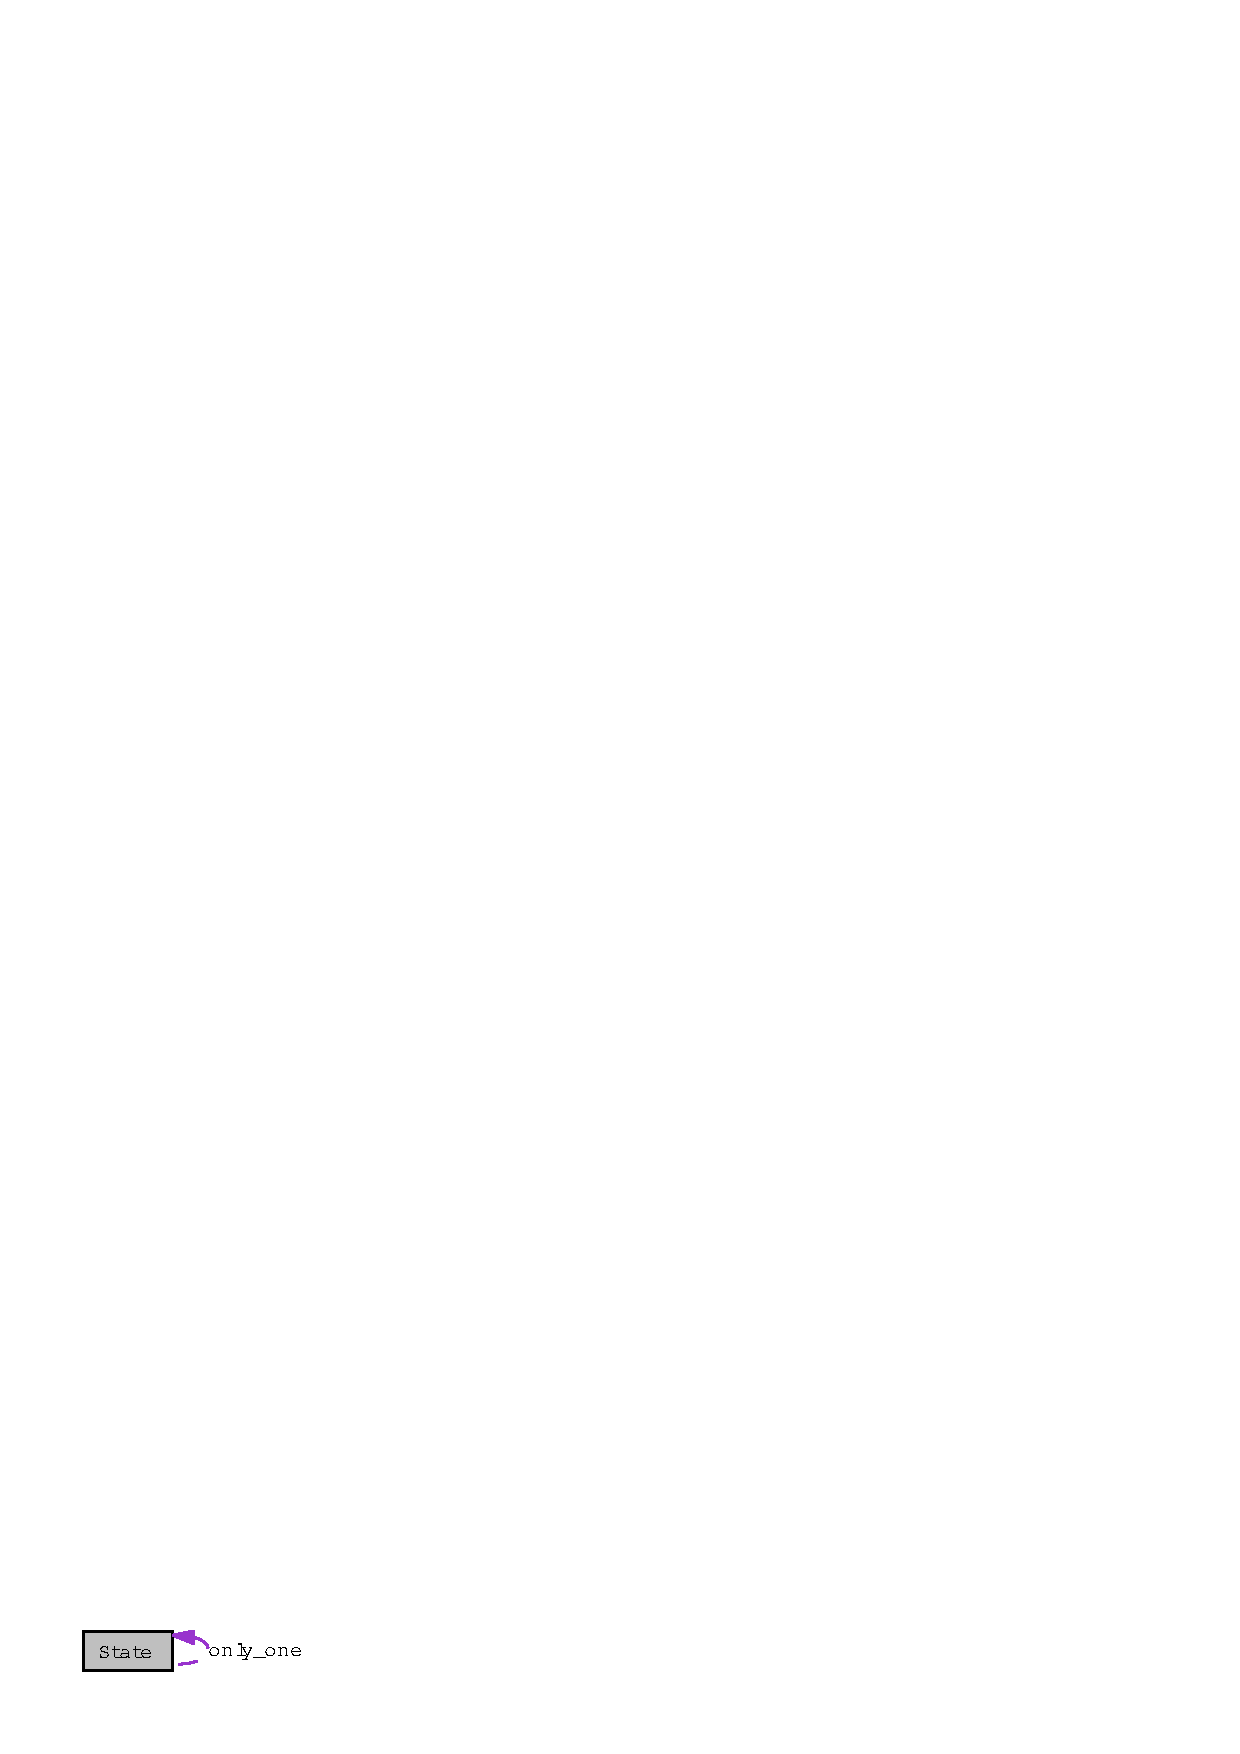
\includegraphics[width=75pt]{classState__coll__graph}
\end{center}
\end{figure}
\subsection*{Public Member Functions}
\begin{CompactItemize}
\item 
{\bf v\_\-set} {\bf get\-Verts\-For\-Full\-Closest\-Pt\-Search} ({\bf Vertex} const $\ast$const, {\bf vector3} const \&, {\bf vector3} const \&)
\item 
{\bf v\_\-set} {\bf get\-Verts\-For\-Partial\-Closest\-Pt\-Search} ({\bf vector3} const \&, {\bf vector3} const \&)
\item 
void {\bf record\-Vert\-Adj\-Face\-Edge\-Angles} ({\bf Vertex} const $\ast$const)
\item 
{\bf Search\_\-Stats} {\bf update\-Closest\-Face\-To\-Vertices} ({\bf Vertex} $\ast$const, {\bf v\_\-set} \&, {\bf v\_\-set} \&)
\item 
void {\bf update\-Adjacent\-Faces\-In\-Tree} ({\bf Vertex} const $\ast$const)
\item 
void {\bf update\-Vertex\-VD} ({\bf Vertex} $\ast$const)
\item 
bool {\bf extreme\-Angle\-Found} (void) const
\item 
bool {\bf assign\-New\-Vertex\-Coords} ({\bf Vertex} $\ast$const, {\bf vector3} const $\ast$const, {\bf vector3} const \&, bool \&, bool \&, bool \&)
\item 
bool {\bf angle\-Change\-Is\-Wrong} (float const \&, float const \&) const
\item 
bool {\bf vertex\-Outside\-Octree\-Bounds} ({\bf vector3} const $\ast$const)
\item 
void {\bf update\-Vertex\-Normals} ({\bf v\_\-set} \&fs)
\item 
void {\bf update\-Adjacent\-Faces\-In\-Octree} ({\bf Vertex} $\ast$const v, {\bf hxa7241\_\-graphics::Vector3r} $\ast$const adjacent\_\-face\_\-lower, {\bf hxa7241\_\-graphics::Vector3r} $\ast$const adjacent\_\-face\_\-upper)
\item 
void {\bf update\-Octree} ({\bf Vertex} $\ast$const v, {\bf hxa7241\_\-graphics::Vector3r} $\ast$const old\_\-adjacent\_\-face\_\-lower, {\bf hxa7241\_\-graphics::Vector3r} $\ast$const old\_\-adjacent\_\-face\_\-upper, {\bf hxa7241\_\-graphics::Vector3r} $\ast$const new\_\-adjacent\_\-face\_\-lower, {\bf hxa7241\_\-graphics::Vector3r} $\ast$const new\_\-adjacent\_\-face\_\-upper)
\item 
float {\bf get\-VD2} (void)
\item 
void {\bf set\-VD2} (float const \&sqd\_\-disp)
\end{CompactItemize}
\subsection*{Static Public Member Functions}
\begin{CompactItemize}
\item 
static {\bf State} \& {\bf instance} (void)
\end{CompactItemize}


\subsection{Member Function Documentation}
\index{State@{State}!instance@{instance}}
\index{instance@{instance}!State@{State}}
\subsubsection{\setlength{\rightskip}{0pt plus 5cm}{\bf State} \& State::instance (void)\hspace{0.3cm}{\tt  [static]}}\label{classState_cd3aa3488c0124d7d4774ff0f7250685}


\index{State@{State}!getVertsForFullClosestPtSearch@{getVertsForFullClosestPtSearch}}
\index{getVertsForFullClosestPtSearch@{getVertsForFullClosestPtSearch}!State@{State}}
\subsubsection{\setlength{\rightskip}{0pt plus 5cm}{\bf v\_\-set} State::get\-Verts\-For\-Full\-Closest\-Pt\-Search ({\bf Vertex} const $\ast$ const {\em v}, {\bf vector3} const \& {\em lower}, {\bf vector3} const \& {\em upper})}\label{classState_79777af274b0b24c635b88ddbe939c28}


Collect vertices whose closest point may now lie anywhere. \begin{Desc}
\item[Parameters:]
\begin{description}
\item[\mbox{$\leftarrow$} {\em v}]The current vertex. \item[\mbox{$\leftarrow$} {\em lower}]Lower corner of desired search region. \item[\mbox{$\leftarrow$} {\em upper}]Upper corner of desired search region. \end{description}
\end{Desc}
\begin{Desc}
\item[Returns:]\doxyref{Vertex}{p.}{classVertex} pointers requiring full closest point search. \end{Desc}
\index{State@{State}!getVertsForPartialClosestPtSearch@{getVertsForPartialClosestPtSearch}}
\index{getVertsForPartialClosestPtSearch@{getVertsForPartialClosestPtSearch}!State@{State}}
\subsubsection{\setlength{\rightskip}{0pt plus 5cm}{\bf v\_\-set} State::get\-Verts\-For\-Partial\-Closest\-Pt\-Search ({\bf vector3} const \& {\em lower}, {\bf vector3} const \& {\em upper})}\label{classState_dc783c8a19fb81acb36dc6985bf14dc7}


Collect vertices whose closest point may now lie on an adjacent face of current vertex.

\begin{Desc}
\item[Parameters:]
\begin{description}
\item[\mbox{$\leftarrow$} {\em lower}]Lower corner of desired search region. \item[\mbox{$\leftarrow$} {\em upper}]Upper corner of desired search region. \end{description}
\end{Desc}
\begin{Desc}
\item[Returns:]\doxyref{Vertex}{p.}{classVertex} pointers requiring partial closest point search. \end{Desc}
\index{State@{State}!recordVertAdjFaceEdgeAngles@{recordVertAdjFaceEdgeAngles}}
\index{recordVertAdjFaceEdgeAngles@{recordVertAdjFaceEdgeAngles}!State@{State}}
\subsubsection{\setlength{\rightskip}{0pt plus 5cm}void State::record\-Vert\-Adj\-Face\-Edge\-Angles ({\bf Vertex} const $\ast$ const {\em v})}\label{classState_2a79e1de329991765d02ade4199e64c8}


Record all edge angles from adjacent faces to input vertex. \begin{Desc}
\item[Parameters:]
\begin{description}
\item[\mbox{$\leftarrow$} {\em v}]\doxyref{Vertex}{p.}{classVertex} of interest. \end{description}
\end{Desc}
\index{State@{State}!updateClosestFaceToVertices@{updateClosestFaceToVertices}}
\index{updateClosestFaceToVertices@{updateClosestFaceToVertices}!State@{State}}
\subsubsection{\setlength{\rightskip}{0pt plus 5cm}{\bf Search\_\-Stats} State::update\-Closest\-Face\-To\-Vertices ({\bf Vertex} $\ast$ const {\em v}, {\bf v\_\-set} \& {\em fs}, {\bf v\_\-set} \& {\em ps})}\label{classState_44c20530fad7b5e4543571b30bdd850d}


Search for new closest point to input vertices.

\begin{Desc}
\item[Parameters:]
\begin{description}
\item[\mbox{$\leftarrow$} {\em v}]The current vertex. \item[\mbox{$\leftarrow$} {\em fs}]Hashed set of vertex pointers requiring full closest point search. \item[\mbox{$\leftarrow$} {\em ps}]Vector of vertex pointers requiring partial closest point search. \end{description}
\end{Desc}
\begin{Desc}
\item[Returns:]Collection of vertex counts quantifying how often the closest face to vertex changed. \end{Desc}
\index{State@{State}!updateAdjacentFacesInTree@{updateAdjacentFacesInTree}}
\index{updateAdjacentFacesInTree@{updateAdjacentFacesInTree}!State@{State}}
\subsubsection{\setlength{\rightskip}{0pt plus 5cm}void State::update\-Adjacent\-Faces\-In\-Tree ({\bf Vertex} const $\ast$ const {\em v})}\label{classState_00e926331052fea5700da67f7d1bb3db}


Update the location of adjacent faces to moved vertex in octree. \begin{Desc}
\item[Parameters:]
\begin{description}
\item[\mbox{$\leftarrow$} {\em v}]Last moved vertex. \end{description}
\end{Desc}
\index{State@{State}!updateVertexVD@{updateVertexVD}}
\index{updateVertexVD@{updateVertexVD}!State@{State}}
\subsubsection{\setlength{\rightskip}{0pt plus 5cm}void State::update\-Vertex\-VD ({\bf Vertex} $\ast$ const {\em v})}\label{classState_8ed5ca2a5be6e2c161240f9caaea80b3}


The virtual displacement of all vertices on adjacent faces of moved vertex will have changed, so update the appropriate maps.

\begin{Desc}
\item[Parameters:]
\begin{description}
\item[\mbox{$\leftarrow$} {\em v}]The current vertex. \end{description}
\end{Desc}
\index{State@{State}!extremeAngleFound@{extremeAngleFound}}
\index{extremeAngleFound@{extremeAngleFound}!State@{State}}
\subsubsection{\setlength{\rightskip}{0pt plus 5cm}bool State::extreme\-Angle\-Found (void) const}\label{classState_06e73d7906137e42ca970187a16e4e0e}


Require vertex move to not worsen the condition of extreme angles. \begin{Desc}
\item[Returns:]True if vertex move is an extreme angle violation; false if move passed the extreme angle test. \end{Desc}
\index{State@{State}!assignNewVertexCoords@{assignNewVertexCoords}}
\index{assignNewVertexCoords@{assignNewVertexCoords}!State@{State}}
\subsubsection{\setlength{\rightskip}{0pt plus 5cm}bool State::assign\-New\-Vertex\-Coords ({\bf Vertex} $\ast$ const {\em v}, {\bf vector3} const $\ast$ const {\em new\_\-pos}, {\bf vector3} const \& {\em old\_\-pos}, bool \& {\em face\_\-intersection}, bool \& {\em extreme\_\-angle}, bool \& {\em outside\_\-octree})}\label{classState_6afda204e91dd271e65a2b1189f4f06a}


Attempt move by input vertex. \begin{Desc}
\item[Parameters:]
\begin{description}
\item[\mbox{$\leftarrow$} {\em v}]\doxyref{Vertex}{p.}{classVertex} to move. \item[\mbox{$\leftarrow$} {\em new\_\-pos}]New location of vertex after move. \item[\mbox{$\rightarrow$} {\em face\_\-intersection}]True if interecting faces were detected and move was aborted. \item[\mbox{$\rightarrow$} {\em extreme\_\-angle}]True if extreme angles (near 0 or 2$\ast$pi) were detected and move was aborted. \item[\mbox{$\rightarrow$} {\em outside\_\-octree}]True if vertex move breached octree boundary and move was aborted. \end{description}
\end{Desc}
\begin{Desc}
\item[Returns:]True if move successful; false otherwise and vertex does not move. \end{Desc}
\index{State@{State}!angleChangeIsWrong@{angleChangeIsWrong}}
\index{angleChangeIsWrong@{angleChangeIsWrong}!State@{State}}
\subsubsection{\setlength{\rightskip}{0pt plus 5cm}bool State::angle\-Change\-Is\-Wrong (float const \& {\em old\_\-angle}, float const \& {\em new\_\-angle}) const}\label{classState_61b50db4d6a224a2275776803f633bc9}


Determine if extreme angle improved. \begin{Desc}
\item[Parameters:]
\begin{description}
\item[\mbox{$\leftarrow$} {\em old\_\-angle}]Extreme angle before the last vertex move. \item[\mbox{$\leftarrow$} {\em new\_\-angle}]Extreme angle after the last vertex move. \end{description}
\end{Desc}
\begin{Desc}
\item[Returns:]False if the change improved the angle; true otherwise. \end{Desc}
\index{State@{State}!vertexOutsideOctreeBounds@{vertexOutsideOctreeBounds}}
\index{vertexOutsideOctreeBounds@{vertexOutsideOctreeBounds}!State@{State}}
\subsubsection{\setlength{\rightskip}{0pt plus 5cm}bool State::vertex\-Outside\-Octree\-Bounds ({\bf vector3} const $\ast$ {\em const})}\label{classState_f7b810832e889c7cd1ac949240ddd099}


\index{State@{State}!updateVertexNormals@{updateVertexNormals}}
\index{updateVertexNormals@{updateVertexNormals}!State@{State}}
\subsubsection{\setlength{\rightskip}{0pt plus 5cm}void State::update\-Vertex\-Normals ({\bf v\_\-set} \& {\em fs})}\label{classState_d79a27db8482298f63e9f5a43ec54a8c}


Update vertex normals of vertices around moved vertex.

\begin{Desc}
\item[Parameters:]
\begin{description}
\item[\mbox{$\leftarrow$} {\em fs}]Hashed set of vertex pointers requiring full closest point search. \end{description}
\end{Desc}
\index{State@{State}!updateAdjacentFacesInOctree@{updateAdjacentFacesInOctree}}
\index{updateAdjacentFacesInOctree@{updateAdjacentFacesInOctree}!State@{State}}
\subsubsection{\setlength{\rightskip}{0pt plus 5cm}void State::update\-Adjacent\-Faces\-In\-Octree ({\bf Vertex} $\ast$const {\em v}, {\bf hxa7241\_\-graphics::Vector3r} $\ast$const {\em adjacent\_\-face\_\-lower}, {\bf hxa7241\_\-graphics::Vector3r} $\ast$const {\em adjacent\_\-face\_\-upper})}\label{classState_f27c97f19211d07041274058804dc0e7}


Update the octree with the new position of input adjacent faces to moved vertex. \begin{Desc}
\item[Parameters:]
\begin{description}
\item[\mbox{$\leftarrow$} {\em v}]Moved vertex. \item[\mbox{$\leftarrow$} {\em adjacent\_\-face\_\-lower}]Pointer to lower corner of pre-move bounding box of first adjacent face to moved vertex. \item[\mbox{$\leftarrow$} {\em adjacent\_\-face\_\-upper}]Pointer to upper corner of pre-move bounding box of first adjacent face to moved vertex. \end{description}
\end{Desc}
\index{State@{State}!updateOctree@{updateOctree}}
\index{updateOctree@{updateOctree}!State@{State}}
\subsubsection{\setlength{\rightskip}{0pt plus 5cm}void State::update\-Octree ({\bf Vertex} $\ast$const {\em v}, {\bf hxa7241\_\-graphics::Vector3r} $\ast$const {\em old\_\-adjacent\_\-face\_\-lower}, {\bf hxa7241\_\-graphics::Vector3r} $\ast$const {\em old\_\-adjacent\_\-face\_\-upper}, {\bf hxa7241\_\-graphics::Vector3r} $\ast$const {\em new\_\-adjacent\_\-face\_\-lower}, {\bf hxa7241\_\-graphics::Vector3r} $\ast$const {\em new\_\-adjacent\_\-face\_\-upper})}\label{classState_3fde06ff5fde9a07028ddcc9f0375da5}


Update the location of moved vertex adjacent faces in the octree. \begin{Desc}
\item[Parameters:]
\begin{description}
\item[\mbox{$\leftarrow$} {\em v}]Moved vertex. \item[\mbox{$\leftarrow$} {\em old\_\-adjacent\_\-face\_\-lower}]Pointer to lower corner of old bounding box of first adjacent face to moved vertex. \item[\mbox{$\leftarrow$} {\em old\_\-adjacent\_\-face\_\-upper}]Pointer to upper corner of old bounding box of first adjacent face to moved vertex. \item[\mbox{$\leftarrow$} {\em new\_\-adjacent\_\-face\_\-lower}]Pointer to lower corner of new bounding box of first adjacent face to moved vertex. \item[\mbox{$\leftarrow$} {\em new\_\-adjacent\_\-face\_\-upper}]Pointer to upper corner of new bounding box of first adjacent face to moved vertex. \end{description}
\end{Desc}
\index{State@{State}!getVD2@{getVD2}}
\index{getVD2@{getVD2}!State@{State}}
\subsubsection{\setlength{\rightskip}{0pt plus 5cm}float State::get\-VD2 (void)\hspace{0.3cm}{\tt  [inline]}}\label{classState_71ce175c245ca2d7925b3ddd9e072f70}


Return stored virtual displacement squared. \begin{Desc}
\item[Returns:]Squared virtual displacement. \end{Desc}
\index{State@{State}!setVD2@{setVD2}}
\index{setVD2@{setVD2}!State@{State}}
\subsubsection{\setlength{\rightskip}{0pt plus 5cm}void State::set\-VD2 (float const \& {\em sqd\_\-disp})\hspace{0.3cm}{\tt  [inline]}}\label{classState_b9acb3ffd6d4945c08f3cf432ed97124}


Set stored virtual displacement squared. \begin{Desc}
\item[Parameters:]
\begin{description}
\item[\mbox{$\leftarrow$} {\em sqd\_\-disp}]Squared virtual displacement. \end{description}
\end{Desc}


The documentation for this class was generated from the following files:\begin{CompactItemize}
\item 
{\bf state.h}\item 
{\bf state.cc}\end{CompactItemize}

\section{Wm4::System Class Reference}
\label{classWm4_1_1System}\index{Wm4::System@{Wm4::System}}
{\tt \#include $<$Wm4System.h$>$}

\subsection*{Public Types}
\begin{CompactItemize}
\item 
enum \{ {\bf SM\_\-READ}, 
{\bf SM\_\-WRITE}, 
{\bf SM\_\-READ\_\-WRITE}
 \}
\end{CompactItemize}
\subsection*{Static Public Member Functions}
\begin{CompactItemize}
\item 
static void {\bf Swap\-Bytes} (int i\-Size, void $\ast$pv\-Value)
\item 
static void {\bf Swap\-Bytes} (int i\-Size, int i\-Quantity, void $\ast$pv\-Value)
\item 
static bool {\bf Is\-Big\-Endian} ()
\item 
static void {\bf Endian\-Copy} (int i\-Size, const void $\ast$pv\-Src, void $\ast$pv\-Dst)
\item 
static void {\bf Endian\-Copy} (int i\-Size, int i\-Quantity, const void $\ast$pv\-Src, void $\ast$pv\-Dst)
\item 
static double {\bf Get\-Time} ()
\item 
static bool {\bf Load} (const char $\ast$ac\-Filename, char $\ast$\&rac\-Buffer, int \&ri\-Size)
\item 
static bool {\bf Save} (const char $\ast$ac\-Filename, const char $\ast$ac\-Buffer, int i\-Size)
\item 
static bool {\bf Append} (const char $\ast$ac\-Filename, char $\ast$ac\-Buffer, int i\-Size)
\item 
static int {\bf Read1} (const char $\ast$ac\-Buffer, int i\-Quantity, void $\ast$pv\-Data)
\item 
static int {\bf Write1} (char $\ast$ac\-Buffer, int i\-Quantity, const void $\ast$pv\-Data)
\item 
static int {\bf Read1} (FILE $\ast$pk\-File, int i\-Quantity, void $\ast$pv\-Data)
\item 
static int {\bf Write1} (FILE $\ast$pk\-File, int i\-Quantity, const void $\ast$pv\-Data)
\item 
static int {\bf Read2le} (const char $\ast$ac\-Buffer, int i\-Quantity, void $\ast$pv\-Data)
\item 
static int {\bf Read4le} (const char $\ast$ac\-Buffer, int i\-Quantity, void $\ast$pv\-Data)
\item 
static int {\bf Read8le} (const char $\ast$ac\-Buffer, int i\-Quantity, void $\ast$pv\-Data)
\item 
static int {\bf Write2le} (char $\ast$ac\-Buffer, int i\-Quantity, const void $\ast$pv\-Data)
\item 
static int {\bf Write4le} (char $\ast$ac\-Buffer, int i\-Quantity, const void $\ast$pv\-Data)
\item 
static int {\bf Write8le} (char $\ast$ac\-Buffer, int i\-Quantity, const void $\ast$pv\-Data)
\item 
static int {\bf Read2le} (FILE $\ast$pk\-File, int i\-Quantity, void $\ast$pv\-Data)
\item 
static int {\bf Read4le} (FILE $\ast$pk\-File, int i\-Quantity, void $\ast$pv\-Data)
\item 
static int {\bf Read8le} (FILE $\ast$pk\-File, int i\-Quantity, void $\ast$pv\-Data)
\item 
static int {\bf Write2le} (FILE $\ast$pk\-File, int i\-Quantity, const void $\ast$pv\-Data)
\item 
static int {\bf Write4le} (FILE $\ast$pk\-File, int i\-Quantity, const void $\ast$pv\-Data)
\item 
static int {\bf Write8le} (FILE $\ast$pk\-File, int i\-Quantity, const void $\ast$pv\-Data)
\item 
static int {\bf Read2be} (const char $\ast$ac\-Buffer, int i\-Quantity, void $\ast$pv\-Data)
\item 
static int {\bf Read4be} (const char $\ast$ac\-Buffer, int i\-Quantity, void $\ast$pv\-Data)
\item 
static int {\bf Read8be} (const char $\ast$ac\-Buffer, int i\-Quantity, void $\ast$pv\-Data)
\item 
static int {\bf Write2be} (char $\ast$ac\-Buffer, int i\-Quantity, const void $\ast$pv\-Data)
\item 
static int {\bf Write4be} (char $\ast$ac\-Buffer, int i\-Quantity, const void $\ast$pv\-Data)
\item 
static int {\bf Write8be} (char $\ast$ac\-Buffer, int i\-Quantity, const void $\ast$pv\-Data)
\item 
static int {\bf Read2be} (FILE $\ast$pk\-File, int i\-Quantity, void $\ast$pv\-Data)
\item 
static int {\bf Read4be} (FILE $\ast$pk\-File, int i\-Quantity, void $\ast$pv\-Data)
\item 
static int {\bf Read8be} (FILE $\ast$pk\-File, int i\-Quantity, void $\ast$pv\-Data)
\item 
static int {\bf Write2be} (FILE $\ast$pk\-File, int i\-Quantity, const void $\ast$pv\-Data)
\item 
static int {\bf Write4be} (FILE $\ast$pk\-File, int i\-Quantity, const void $\ast$pv\-Data)
\item 
static int {\bf Write8be} (FILE $\ast$pk\-File, int i\-Quantity, const void $\ast$pv\-Data)
\item 
static const char $\ast$ {\bf Get\-Path} (const char $\ast$ac\-Directory, const char $\ast$ac\-Filename)
\item 
static void {\bf Initialize} ()
\item 
static void {\bf Terminate} ()
\item 
static int {\bf Get\-Directory\-Quantity} ()
\item 
static const char $\ast$ {\bf Get\-Directory} (int i)
\item 
static bool {\bf Insert\-Directory} (const char $\ast$ac\-Directory)
\item 
static bool {\bf Remove\-Directory} (const char $\ast$ac\-Directory)
\item 
static void {\bf Remove\-All\-Directories} ()
\item 
static const char $\ast$ {\bf Get\-Path} (const char $\ast$ac\-Filename, int e\-Mode)
\item 
static unsigned int {\bf Make\-RGB} (unsigned char uc\-R, unsigned char uc\-G, unsigned char uc\-B)
\item 
static unsigned int {\bf Make\-RGBA} (unsigned char uc\-R, unsigned char uc\-G, unsigned char uc\-B, unsigned char uc\-A)
\item 
static FILE $\ast$ {\bf Fopen} (const char $\ast$ac\-Filename, const char $\ast$ac\-Mode)
\item 
static int {\bf Fprintf} (FILE $\ast$pk\-File, const char $\ast$ac\-Format,...)
\item 
static int {\bf Fclose} (FILE $\ast$pk\-File)
\item 
static const char $\ast$ {\bf Get\-Env} (const char $\ast$ac\-Env\-Var\-Name)
\item 
static void $\ast$ {\bf Memcpy} (void $\ast$pv\-Dst, size\_\-t ui\-Dst\-Size, const void $\ast$pv\-Src, size\_\-t ui\-Src\-Size)
\item 
static int {\bf Sprintf} (char $\ast$ac\-Dst, size\_\-t ui\-Dst\-Size, const char $\ast$ac\-Format,...)
\item 
static char $\ast$ {\bf Strcpy} (char $\ast$ac\-Dst, size\_\-t ui\-Dst\-Size, const char $\ast$ac\-Src)
\item 
static char $\ast$ {\bf Strcat} (char $\ast$ac\-Dst, size\_\-t ui\-Dst\-Size, const char $\ast$ac\-Src)
\item 
static char $\ast$ {\bf Strncpy} (char $\ast$ac\-Dst, size\_\-t ui\-Dst\-Size, const char $\ast$ac\-Src, size\_\-t ui\-Src\-Size)
\item 
static char $\ast$ {\bf Strtok} (char $\ast$ac\-Token, const char $\ast$ac\-Delimiters, char $\ast$\&rac\-Next\-Token)
\end{CompactItemize}
\subsection*{Static Public Attributes}
\begin{CompactItemize}
\item 
static char {\bf WM4\_\-PATH} [SYSTEM\_\-MAX\_\-ENVVAR]
\end{CompactItemize}


\subsection{Member Enumeration Documentation}
\subsubsection{\setlength{\rightskip}{0pt plus 5cm}anonymous enum}\label{classWm4_1_1System_7737a7e47a84d48b2227363f47e4fd48}


\begin{Desc}
\item[Enumerator: ]\par
\begin{description}
\index{SM_READ@{SM\_\-READ}!Wm4::System@{Wm4::System}}\index{Wm4::System@{Wm4::System}!SM_READ@{SM\_\-READ}}\item[{\em 
SM\_\-READ\label{classWm4_1_1System_7737a7e47a84d48b2227363f47e4fd4886b04bdaa52a6e54405cb1cb26a3c346}
}]\index{SM_WRITE@{SM\_\-WRITE}!Wm4::System@{Wm4::System}}\index{Wm4::System@{Wm4::System}!SM_WRITE@{SM\_\-WRITE}}\item[{\em 
SM\_\-WRITE\label{classWm4_1_1System_7737a7e47a84d48b2227363f47e4fd4834a821d0dafc541253bfa7f690603c20}
}]\index{SM_READ_WRITE@{SM\_\-READ\_\-WRITE}!Wm4::System@{Wm4::System}}\index{Wm4::System@{Wm4::System}!SM_READ_WRITE@{SM\_\-READ\_\-WRITE}}\item[{\em 
SM\_\-READ\_\-WRITE\label{classWm4_1_1System_7737a7e47a84d48b2227363f47e4fd487280e99bb81b1391b371f31a9b0e1c3c}
}]\end{description}
\end{Desc}



\subsection{Member Function Documentation}
\index{Wm4::System@{Wm4::System}!SwapBytes@{SwapBytes}}
\index{SwapBytes@{SwapBytes}!Wm4::System@{Wm4::System}}
\subsubsection{\setlength{\rightskip}{0pt plus 5cm}static void Wm4::System::Swap\-Bytes (int {\em i\-Size}, void $\ast$ {\em pv\-Value})\hspace{0.3cm}{\tt  [static]}}\label{classWm4_1_1System_3e986994800c78c70f2a7f007084754a}


\index{Wm4::System@{Wm4::System}!SwapBytes@{SwapBytes}}
\index{SwapBytes@{SwapBytes}!Wm4::System@{Wm4::System}}
\subsubsection{\setlength{\rightskip}{0pt plus 5cm}static void Wm4::System::Swap\-Bytes (int {\em i\-Size}, int {\em i\-Quantity}, void $\ast$ {\em pv\-Value})\hspace{0.3cm}{\tt  [static]}}\label{classWm4_1_1System_4d72f4992514ce404cd4896f1fdc8aa4}


\index{Wm4::System@{Wm4::System}!IsBigEndian@{IsBigEndian}}
\index{IsBigEndian@{IsBigEndian}!Wm4::System@{Wm4::System}}
\subsubsection{\setlength{\rightskip}{0pt plus 5cm}static bool Wm4::System::Is\-Big\-Endian ()\hspace{0.3cm}{\tt  [static]}}\label{classWm4_1_1System_8a732286323936a8d1b259dcbadbb840}


\index{Wm4::System@{Wm4::System}!EndianCopy@{EndianCopy}}
\index{EndianCopy@{EndianCopy}!Wm4::System@{Wm4::System}}
\subsubsection{\setlength{\rightskip}{0pt plus 5cm}static void Wm4::System::Endian\-Copy (int {\em i\-Size}, const void $\ast$ {\em pv\-Src}, void $\ast$ {\em pv\-Dst})\hspace{0.3cm}{\tt  [static]}}\label{classWm4_1_1System_90f08ebd7dd7af09479e1277f7126523}


\index{Wm4::System@{Wm4::System}!EndianCopy@{EndianCopy}}
\index{EndianCopy@{EndianCopy}!Wm4::System@{Wm4::System}}
\subsubsection{\setlength{\rightskip}{0pt plus 5cm}static void Wm4::System::Endian\-Copy (int {\em i\-Size}, int {\em i\-Quantity}, const void $\ast$ {\em pv\-Src}, void $\ast$ {\em pv\-Dst})\hspace{0.3cm}{\tt  [static]}}\label{classWm4_1_1System_8245e37e2d2f5a98788106e242e6277d}


\index{Wm4::System@{Wm4::System}!GetTime@{GetTime}}
\index{GetTime@{GetTime}!Wm4::System@{Wm4::System}}
\subsubsection{\setlength{\rightskip}{0pt plus 5cm}static double Wm4::System::Get\-Time ()\hspace{0.3cm}{\tt  [static]}}\label{classWm4_1_1System_3ff19ffa86de311957c3b94fc4c86197}


\index{Wm4::System@{Wm4::System}!Load@{Load}}
\index{Load@{Load}!Wm4::System@{Wm4::System}}
\subsubsection{\setlength{\rightskip}{0pt plus 5cm}static bool Wm4::System::Load (const char $\ast$ {\em ac\-Filename}, char $\ast$\& {\em rac\-Buffer}, int \& {\em ri\-Size})\hspace{0.3cm}{\tt  [static]}}\label{classWm4_1_1System_af5d5efbf10c46fe611bfc7244594476}


\index{Wm4::System@{Wm4::System}!Save@{Save}}
\index{Save@{Save}!Wm4::System@{Wm4::System}}
\subsubsection{\setlength{\rightskip}{0pt plus 5cm}static bool Wm4::System::Save (const char $\ast$ {\em ac\-Filename}, const char $\ast$ {\em ac\-Buffer}, int {\em i\-Size})\hspace{0.3cm}{\tt  [static]}}\label{classWm4_1_1System_77e0c4429d584c7e2e3cc8dd6f56c96e}


\index{Wm4::System@{Wm4::System}!Append@{Append}}
\index{Append@{Append}!Wm4::System@{Wm4::System}}
\subsubsection{\setlength{\rightskip}{0pt plus 5cm}static bool Wm4::System::Append (const char $\ast$ {\em ac\-Filename}, char $\ast$ {\em ac\-Buffer}, int {\em i\-Size})\hspace{0.3cm}{\tt  [static]}}\label{classWm4_1_1System_45f7cb9f567a6bbb3aeab9d5318973f3}


\index{Wm4::System@{Wm4::System}!Read1@{Read1}}
\index{Read1@{Read1}!Wm4::System@{Wm4::System}}
\subsubsection{\setlength{\rightskip}{0pt plus 5cm}static int Wm4::System::Read1 (const char $\ast$ {\em ac\-Buffer}, int {\em i\-Quantity}, void $\ast$ {\em pv\-Data})\hspace{0.3cm}{\tt  [static]}}\label{classWm4_1_1System_9f9e56476a8ba5713d2bb2decb4a4ff3}


\index{Wm4::System@{Wm4::System}!Write1@{Write1}}
\index{Write1@{Write1}!Wm4::System@{Wm4::System}}
\subsubsection{\setlength{\rightskip}{0pt plus 5cm}static int Wm4::System::Write1 (char $\ast$ {\em ac\-Buffer}, int {\em i\-Quantity}, const void $\ast$ {\em pv\-Data})\hspace{0.3cm}{\tt  [static]}}\label{classWm4_1_1System_bfaa3ba89083f2366e1ed9d8c69989da}


\index{Wm4::System@{Wm4::System}!Read1@{Read1}}
\index{Read1@{Read1}!Wm4::System@{Wm4::System}}
\subsubsection{\setlength{\rightskip}{0pt plus 5cm}static int Wm4::System::Read1 (FILE $\ast$ {\em pk\-File}, int {\em i\-Quantity}, void $\ast$ {\em pv\-Data})\hspace{0.3cm}{\tt  [static]}}\label{classWm4_1_1System_da908e9cee1c5b0bf03226c0e6962903}


\index{Wm4::System@{Wm4::System}!Write1@{Write1}}
\index{Write1@{Write1}!Wm4::System@{Wm4::System}}
\subsubsection{\setlength{\rightskip}{0pt plus 5cm}static int Wm4::System::Write1 (FILE $\ast$ {\em pk\-File}, int {\em i\-Quantity}, const void $\ast$ {\em pv\-Data})\hspace{0.3cm}{\tt  [static]}}\label{classWm4_1_1System_7946715d85089968263403237a26a2d8}


\index{Wm4::System@{Wm4::System}!Read2le@{Read2le}}
\index{Read2le@{Read2le}!Wm4::System@{Wm4::System}}
\subsubsection{\setlength{\rightskip}{0pt plus 5cm}static int Wm4::System::Read2le (const char $\ast$ {\em ac\-Buffer}, int {\em i\-Quantity}, void $\ast$ {\em pv\-Data})\hspace{0.3cm}{\tt  [static]}}\label{classWm4_1_1System_f0cfb2eb4eb6ed377cfa931e1ee5e638}


\index{Wm4::System@{Wm4::System}!Read4le@{Read4le}}
\index{Read4le@{Read4le}!Wm4::System@{Wm4::System}}
\subsubsection{\setlength{\rightskip}{0pt plus 5cm}static int Wm4::System::Read4le (const char $\ast$ {\em ac\-Buffer}, int {\em i\-Quantity}, void $\ast$ {\em pv\-Data})\hspace{0.3cm}{\tt  [static]}}\label{classWm4_1_1System_f6479ef6fa649750609932f07306f94d}


\index{Wm4::System@{Wm4::System}!Read8le@{Read8le}}
\index{Read8le@{Read8le}!Wm4::System@{Wm4::System}}
\subsubsection{\setlength{\rightskip}{0pt plus 5cm}static int Wm4::System::Read8le (const char $\ast$ {\em ac\-Buffer}, int {\em i\-Quantity}, void $\ast$ {\em pv\-Data})\hspace{0.3cm}{\tt  [static]}}\label{classWm4_1_1System_8d67e3b6439180d7a224bca9f18b54e7}


\index{Wm4::System@{Wm4::System}!Write2le@{Write2le}}
\index{Write2le@{Write2le}!Wm4::System@{Wm4::System}}
\subsubsection{\setlength{\rightskip}{0pt plus 5cm}static int Wm4::System::Write2le (char $\ast$ {\em ac\-Buffer}, int {\em i\-Quantity}, const void $\ast$ {\em pv\-Data})\hspace{0.3cm}{\tt  [static]}}\label{classWm4_1_1System_c570e6b935a363025d4868b03bc3add3}


\index{Wm4::System@{Wm4::System}!Write4le@{Write4le}}
\index{Write4le@{Write4le}!Wm4::System@{Wm4::System}}
\subsubsection{\setlength{\rightskip}{0pt plus 5cm}static int Wm4::System::Write4le (char $\ast$ {\em ac\-Buffer}, int {\em i\-Quantity}, const void $\ast$ {\em pv\-Data})\hspace{0.3cm}{\tt  [static]}}\label{classWm4_1_1System_c988a64a8106c3576b6633210a3d14f8}


\index{Wm4::System@{Wm4::System}!Write8le@{Write8le}}
\index{Write8le@{Write8le}!Wm4::System@{Wm4::System}}
\subsubsection{\setlength{\rightskip}{0pt plus 5cm}static int Wm4::System::Write8le (char $\ast$ {\em ac\-Buffer}, int {\em i\-Quantity}, const void $\ast$ {\em pv\-Data})\hspace{0.3cm}{\tt  [static]}}\label{classWm4_1_1System_b589c5bb09a8147b5dacb2b3eab0cd7e}


\index{Wm4::System@{Wm4::System}!Read2le@{Read2le}}
\index{Read2le@{Read2le}!Wm4::System@{Wm4::System}}
\subsubsection{\setlength{\rightskip}{0pt plus 5cm}static int Wm4::System::Read2le (FILE $\ast$ {\em pk\-File}, int {\em i\-Quantity}, void $\ast$ {\em pv\-Data})\hspace{0.3cm}{\tt  [static]}}\label{classWm4_1_1System_26bb4792ee2fd1dce6eda4971f0d6f1a}


\index{Wm4::System@{Wm4::System}!Read4le@{Read4le}}
\index{Read4le@{Read4le}!Wm4::System@{Wm4::System}}
\subsubsection{\setlength{\rightskip}{0pt plus 5cm}static int Wm4::System::Read4le (FILE $\ast$ {\em pk\-File}, int {\em i\-Quantity}, void $\ast$ {\em pv\-Data})\hspace{0.3cm}{\tt  [static]}}\label{classWm4_1_1System_dc76d8a490eb3834c5b9dfa48893aa0c}


\index{Wm4::System@{Wm4::System}!Read8le@{Read8le}}
\index{Read8le@{Read8le}!Wm4::System@{Wm4::System}}
\subsubsection{\setlength{\rightskip}{0pt plus 5cm}static int Wm4::System::Read8le (FILE $\ast$ {\em pk\-File}, int {\em i\-Quantity}, void $\ast$ {\em pv\-Data})\hspace{0.3cm}{\tt  [static]}}\label{classWm4_1_1System_66b7a25e5e0371fdd8b7fe9865178062}


\index{Wm4::System@{Wm4::System}!Write2le@{Write2le}}
\index{Write2le@{Write2le}!Wm4::System@{Wm4::System}}
\subsubsection{\setlength{\rightskip}{0pt plus 5cm}static int Wm4::System::Write2le (FILE $\ast$ {\em pk\-File}, int {\em i\-Quantity}, const void $\ast$ {\em pv\-Data})\hspace{0.3cm}{\tt  [static]}}\label{classWm4_1_1System_275fc9aed7d3612cec1d478479276881}


\index{Wm4::System@{Wm4::System}!Write4le@{Write4le}}
\index{Write4le@{Write4le}!Wm4::System@{Wm4::System}}
\subsubsection{\setlength{\rightskip}{0pt plus 5cm}static int Wm4::System::Write4le (FILE $\ast$ {\em pk\-File}, int {\em i\-Quantity}, const void $\ast$ {\em pv\-Data})\hspace{0.3cm}{\tt  [static]}}\label{classWm4_1_1System_6538bb9a6eb49b0c8943fccc5ddc6043}


\index{Wm4::System@{Wm4::System}!Write8le@{Write8le}}
\index{Write8le@{Write8le}!Wm4::System@{Wm4::System}}
\subsubsection{\setlength{\rightskip}{0pt plus 5cm}static int Wm4::System::Write8le (FILE $\ast$ {\em pk\-File}, int {\em i\-Quantity}, const void $\ast$ {\em pv\-Data})\hspace{0.3cm}{\tt  [static]}}\label{classWm4_1_1System_f2407893730726f21d896686b902fb4e}


\index{Wm4::System@{Wm4::System}!Read2be@{Read2be}}
\index{Read2be@{Read2be}!Wm4::System@{Wm4::System}}
\subsubsection{\setlength{\rightskip}{0pt plus 5cm}static int Wm4::System::Read2be (const char $\ast$ {\em ac\-Buffer}, int {\em i\-Quantity}, void $\ast$ {\em pv\-Data})\hspace{0.3cm}{\tt  [static]}}\label{classWm4_1_1System_54471c1acd0185a2169f39c1f04e2117}


\index{Wm4::System@{Wm4::System}!Read4be@{Read4be}}
\index{Read4be@{Read4be}!Wm4::System@{Wm4::System}}
\subsubsection{\setlength{\rightskip}{0pt plus 5cm}static int Wm4::System::Read4be (const char $\ast$ {\em ac\-Buffer}, int {\em i\-Quantity}, void $\ast$ {\em pv\-Data})\hspace{0.3cm}{\tt  [static]}}\label{classWm4_1_1System_cfd87f4e948a4acfb9c92d5cfe6bd0cb}


\index{Wm4::System@{Wm4::System}!Read8be@{Read8be}}
\index{Read8be@{Read8be}!Wm4::System@{Wm4::System}}
\subsubsection{\setlength{\rightskip}{0pt plus 5cm}static int Wm4::System::Read8be (const char $\ast$ {\em ac\-Buffer}, int {\em i\-Quantity}, void $\ast$ {\em pv\-Data})\hspace{0.3cm}{\tt  [static]}}\label{classWm4_1_1System_dbc9deaf9ab9d95a76c6d649e7c1ad12}


\index{Wm4::System@{Wm4::System}!Write2be@{Write2be}}
\index{Write2be@{Write2be}!Wm4::System@{Wm4::System}}
\subsubsection{\setlength{\rightskip}{0pt plus 5cm}static int Wm4::System::Write2be (char $\ast$ {\em ac\-Buffer}, int {\em i\-Quantity}, const void $\ast$ {\em pv\-Data})\hspace{0.3cm}{\tt  [static]}}\label{classWm4_1_1System_21d3c0454ee85d06350276f15326f06f}


\index{Wm4::System@{Wm4::System}!Write4be@{Write4be}}
\index{Write4be@{Write4be}!Wm4::System@{Wm4::System}}
\subsubsection{\setlength{\rightskip}{0pt plus 5cm}static int Wm4::System::Write4be (char $\ast$ {\em ac\-Buffer}, int {\em i\-Quantity}, const void $\ast$ {\em pv\-Data})\hspace{0.3cm}{\tt  [static]}}\label{classWm4_1_1System_3a6684f9f1ea57ed7707dd4d4803af75}


\index{Wm4::System@{Wm4::System}!Write8be@{Write8be}}
\index{Write8be@{Write8be}!Wm4::System@{Wm4::System}}
\subsubsection{\setlength{\rightskip}{0pt plus 5cm}static int Wm4::System::Write8be (char $\ast$ {\em ac\-Buffer}, int {\em i\-Quantity}, const void $\ast$ {\em pv\-Data})\hspace{0.3cm}{\tt  [static]}}\label{classWm4_1_1System_dc67e1bcf6743863281c279fd1a990ad}


\index{Wm4::System@{Wm4::System}!Read2be@{Read2be}}
\index{Read2be@{Read2be}!Wm4::System@{Wm4::System}}
\subsubsection{\setlength{\rightskip}{0pt plus 5cm}static int Wm4::System::Read2be (FILE $\ast$ {\em pk\-File}, int {\em i\-Quantity}, void $\ast$ {\em pv\-Data})\hspace{0.3cm}{\tt  [static]}}\label{classWm4_1_1System_fea3a45fc47a19ae287c92799e1ae67c}


\index{Wm4::System@{Wm4::System}!Read4be@{Read4be}}
\index{Read4be@{Read4be}!Wm4::System@{Wm4::System}}
\subsubsection{\setlength{\rightskip}{0pt plus 5cm}static int Wm4::System::Read4be (FILE $\ast$ {\em pk\-File}, int {\em i\-Quantity}, void $\ast$ {\em pv\-Data})\hspace{0.3cm}{\tt  [static]}}\label{classWm4_1_1System_366ff49f9a2af7f14c99d65a0366215f}


\index{Wm4::System@{Wm4::System}!Read8be@{Read8be}}
\index{Read8be@{Read8be}!Wm4::System@{Wm4::System}}
\subsubsection{\setlength{\rightskip}{0pt plus 5cm}static int Wm4::System::Read8be (FILE $\ast$ {\em pk\-File}, int {\em i\-Quantity}, void $\ast$ {\em pv\-Data})\hspace{0.3cm}{\tt  [static]}}\label{classWm4_1_1System_c140bcbc5b9cc63099dc09c5c86fde27}


\index{Wm4::System@{Wm4::System}!Write2be@{Write2be}}
\index{Write2be@{Write2be}!Wm4::System@{Wm4::System}}
\subsubsection{\setlength{\rightskip}{0pt plus 5cm}static int Wm4::System::Write2be (FILE $\ast$ {\em pk\-File}, int {\em i\-Quantity}, const void $\ast$ {\em pv\-Data})\hspace{0.3cm}{\tt  [static]}}\label{classWm4_1_1System_6b0f65a93d1de6b622157ee753bb0d3b}


\index{Wm4::System@{Wm4::System}!Write4be@{Write4be}}
\index{Write4be@{Write4be}!Wm4::System@{Wm4::System}}
\subsubsection{\setlength{\rightskip}{0pt plus 5cm}static int Wm4::System::Write4be (FILE $\ast$ {\em pk\-File}, int {\em i\-Quantity}, const void $\ast$ {\em pv\-Data})\hspace{0.3cm}{\tt  [static]}}\label{classWm4_1_1System_c0bd859fe6d7c7fed6011972f3a8f25d}


\index{Wm4::System@{Wm4::System}!Write8be@{Write8be}}
\index{Write8be@{Write8be}!Wm4::System@{Wm4::System}}
\subsubsection{\setlength{\rightskip}{0pt plus 5cm}static int Wm4::System::Write8be (FILE $\ast$ {\em pk\-File}, int {\em i\-Quantity}, const void $\ast$ {\em pv\-Data})\hspace{0.3cm}{\tt  [static]}}\label{classWm4_1_1System_12e360c02ed2e8b5a4678e9c7863fdfc}


\index{Wm4::System@{Wm4::System}!GetPath@{GetPath}}
\index{GetPath@{GetPath}!Wm4::System@{Wm4::System}}
\subsubsection{\setlength{\rightskip}{0pt plus 5cm}static const char$\ast$ Wm4::System::Get\-Path (const char $\ast$ {\em ac\-Directory}, const char $\ast$ {\em ac\-Filename})\hspace{0.3cm}{\tt  [static]}}\label{classWm4_1_1System_ba1a3ad9c15046b09b96ebf9c417bb77}


\index{Wm4::System@{Wm4::System}!Initialize@{Initialize}}
\index{Initialize@{Initialize}!Wm4::System@{Wm4::System}}
\subsubsection{\setlength{\rightskip}{0pt plus 5cm}static void Wm4::System::Initialize ()\hspace{0.3cm}{\tt  [static]}}\label{classWm4_1_1System_bea72076bb9d98b8c817476740d03718}


\index{Wm4::System@{Wm4::System}!Terminate@{Terminate}}
\index{Terminate@{Terminate}!Wm4::System@{Wm4::System}}
\subsubsection{\setlength{\rightskip}{0pt plus 5cm}static void Wm4::System::Terminate ()\hspace{0.3cm}{\tt  [static]}}\label{classWm4_1_1System_2af0be3481afbb3437c0c9beb6db374f}


\index{Wm4::System@{Wm4::System}!GetDirectoryQuantity@{GetDirectoryQuantity}}
\index{GetDirectoryQuantity@{GetDirectoryQuantity}!Wm4::System@{Wm4::System}}
\subsubsection{\setlength{\rightskip}{0pt plus 5cm}static int Wm4::System::Get\-Directory\-Quantity ()\hspace{0.3cm}{\tt  [static]}}\label{classWm4_1_1System_ffc2a18e5e7c4ea55b34f92e69af78e0}


\index{Wm4::System@{Wm4::System}!GetDirectory@{GetDirectory}}
\index{GetDirectory@{GetDirectory}!Wm4::System@{Wm4::System}}
\subsubsection{\setlength{\rightskip}{0pt plus 5cm}static const char$\ast$ Wm4::System::Get\-Directory (int {\em i})\hspace{0.3cm}{\tt  [static]}}\label{classWm4_1_1System_c1e6ab9941de99aae04751a9b610f97e}


\index{Wm4::System@{Wm4::System}!InsertDirectory@{InsertDirectory}}
\index{InsertDirectory@{InsertDirectory}!Wm4::System@{Wm4::System}}
\subsubsection{\setlength{\rightskip}{0pt plus 5cm}static bool Wm4::System::Insert\-Directory (const char $\ast$ {\em ac\-Directory})\hspace{0.3cm}{\tt  [static]}}\label{classWm4_1_1System_846d953512c67c10518063f303e75f58}


\index{Wm4::System@{Wm4::System}!RemoveDirectory@{RemoveDirectory}}
\index{RemoveDirectory@{RemoveDirectory}!Wm4::System@{Wm4::System}}
\subsubsection{\setlength{\rightskip}{0pt plus 5cm}static bool Wm4::System::Remove\-Directory (const char $\ast$ {\em ac\-Directory})\hspace{0.3cm}{\tt  [static]}}\label{classWm4_1_1System_40219b7af70b4e3e82c39142cfb7a43c}


\index{Wm4::System@{Wm4::System}!RemoveAllDirectories@{RemoveAllDirectories}}
\index{RemoveAllDirectories@{RemoveAllDirectories}!Wm4::System@{Wm4::System}}
\subsubsection{\setlength{\rightskip}{0pt plus 5cm}static void Wm4::System::Remove\-All\-Directories ()\hspace{0.3cm}{\tt  [static]}}\label{classWm4_1_1System_69c5a8fe084676959254ab8e8e553c69}


\index{Wm4::System@{Wm4::System}!GetPath@{GetPath}}
\index{GetPath@{GetPath}!Wm4::System@{Wm4::System}}
\subsubsection{\setlength{\rightskip}{0pt plus 5cm}static const char$\ast$ Wm4::System::Get\-Path (const char $\ast$ {\em ac\-Filename}, int {\em e\-Mode})\hspace{0.3cm}{\tt  [static]}}\label{classWm4_1_1System_6b85cc5e27250e080242e53a2d70f43e}


\index{Wm4::System@{Wm4::System}!MakeRGB@{MakeRGB}}
\index{MakeRGB@{MakeRGB}!Wm4::System@{Wm4::System}}
\subsubsection{\setlength{\rightskip}{0pt plus 5cm}static unsigned int Wm4::System::Make\-RGB (unsigned char {\em uc\-R}, unsigned char {\em uc\-G}, unsigned char {\em uc\-B})\hspace{0.3cm}{\tt  [static]}}\label{classWm4_1_1System_8fca5bb438de73f2f9e179257e874278}


\index{Wm4::System@{Wm4::System}!MakeRGBA@{MakeRGBA}}
\index{MakeRGBA@{MakeRGBA}!Wm4::System@{Wm4::System}}
\subsubsection{\setlength{\rightskip}{0pt plus 5cm}static unsigned int Wm4::System::Make\-RGBA (unsigned char {\em uc\-R}, unsigned char {\em uc\-G}, unsigned char {\em uc\-B}, unsigned char {\em uc\-A})\hspace{0.3cm}{\tt  [static]}}\label{classWm4_1_1System_eab6285f19bd417da080e5e0feca3632}


\index{Wm4::System@{Wm4::System}!Fopen@{Fopen}}
\index{Fopen@{Fopen}!Wm4::System@{Wm4::System}}
\subsubsection{\setlength{\rightskip}{0pt plus 5cm}static FILE$\ast$ Wm4::System::Fopen (const char $\ast$ {\em ac\-Filename}, const char $\ast$ {\em ac\-Mode})\hspace{0.3cm}{\tt  [static]}}\label{classWm4_1_1System_340806bcae5d85bb9eea6a38f3df84b8}


\index{Wm4::System@{Wm4::System}!Fprintf@{Fprintf}}
\index{Fprintf@{Fprintf}!Wm4::System@{Wm4::System}}
\subsubsection{\setlength{\rightskip}{0pt plus 5cm}static int Wm4::System::Fprintf (FILE $\ast$ {\em pk\-File}, const char $\ast$ {\em ac\-Format},  {\em ...})\hspace{0.3cm}{\tt  [static]}}\label{classWm4_1_1System_7a8fee165f061ee53c229cb37643574c}


\index{Wm4::System@{Wm4::System}!Fclose@{Fclose}}
\index{Fclose@{Fclose}!Wm4::System@{Wm4::System}}
\subsubsection{\setlength{\rightskip}{0pt plus 5cm}static int Wm4::System::Fclose (FILE $\ast$ {\em pk\-File})\hspace{0.3cm}{\tt  [static]}}\label{classWm4_1_1System_fe63864b7d95be12e38287758bc3cbb9}


\index{Wm4::System@{Wm4::System}!GetEnv@{GetEnv}}
\index{GetEnv@{GetEnv}!Wm4::System@{Wm4::System}}
\subsubsection{\setlength{\rightskip}{0pt plus 5cm}static const char$\ast$ Wm4::System::Get\-Env (const char $\ast$ {\em ac\-Env\-Var\-Name})\hspace{0.3cm}{\tt  [static]}}\label{classWm4_1_1System_49cd19097e976c709101789c3a7582c7}


\index{Wm4::System@{Wm4::System}!Memcpy@{Memcpy}}
\index{Memcpy@{Memcpy}!Wm4::System@{Wm4::System}}
\subsubsection{\setlength{\rightskip}{0pt plus 5cm}static void$\ast$ Wm4::System::Memcpy (void $\ast$ {\em pv\-Dst}, size\_\-t {\em ui\-Dst\-Size}, const void $\ast$ {\em pv\-Src}, size\_\-t {\em ui\-Src\-Size})\hspace{0.3cm}{\tt  [static]}}\label{classWm4_1_1System_eb8cad2018a4ca7c66012a41bea165ad}


\index{Wm4::System@{Wm4::System}!Sprintf@{Sprintf}}
\index{Sprintf@{Sprintf}!Wm4::System@{Wm4::System}}
\subsubsection{\setlength{\rightskip}{0pt plus 5cm}static int Wm4::System::Sprintf (char $\ast$ {\em ac\-Dst}, size\_\-t {\em ui\-Dst\-Size}, const char $\ast$ {\em ac\-Format},  {\em ...})\hspace{0.3cm}{\tt  [static]}}\label{classWm4_1_1System_8ea0b5ef972230ec66b1d0ad888060f4}


\index{Wm4::System@{Wm4::System}!Strcpy@{Strcpy}}
\index{Strcpy@{Strcpy}!Wm4::System@{Wm4::System}}
\subsubsection{\setlength{\rightskip}{0pt plus 5cm}static char$\ast$ Wm4::System::Strcpy (char $\ast$ {\em ac\-Dst}, size\_\-t {\em ui\-Dst\-Size}, const char $\ast$ {\em ac\-Src})\hspace{0.3cm}{\tt  [static]}}\label{classWm4_1_1System_76871a39455735cfb870f0bd2334655b}


\index{Wm4::System@{Wm4::System}!Strcat@{Strcat}}
\index{Strcat@{Strcat}!Wm4::System@{Wm4::System}}
\subsubsection{\setlength{\rightskip}{0pt plus 5cm}static char$\ast$ Wm4::System::Strcat (char $\ast$ {\em ac\-Dst}, size\_\-t {\em ui\-Dst\-Size}, const char $\ast$ {\em ac\-Src})\hspace{0.3cm}{\tt  [static]}}\label{classWm4_1_1System_f4448e643b507d29fa12a801f6e73486}


\index{Wm4::System@{Wm4::System}!Strncpy@{Strncpy}}
\index{Strncpy@{Strncpy}!Wm4::System@{Wm4::System}}
\subsubsection{\setlength{\rightskip}{0pt plus 5cm}static char$\ast$ Wm4::System::Strncpy (char $\ast$ {\em ac\-Dst}, size\_\-t {\em ui\-Dst\-Size}, const char $\ast$ {\em ac\-Src}, size\_\-t {\em ui\-Src\-Size})\hspace{0.3cm}{\tt  [static]}}\label{classWm4_1_1System_662413b41fda59780384142ed6cbb7a0}


\index{Wm4::System@{Wm4::System}!Strtok@{Strtok}}
\index{Strtok@{Strtok}!Wm4::System@{Wm4::System}}
\subsubsection{\setlength{\rightskip}{0pt plus 5cm}static char$\ast$ Wm4::System::Strtok (char $\ast$ {\em ac\-Token}, const char $\ast$ {\em ac\-Delimiters}, char $\ast$\& {\em rac\-Next\-Token})\hspace{0.3cm}{\tt  [static]}}\label{classWm4_1_1System_323f5f05e9ec0049dbbbb88563bb99c5}




\subsection{Member Data Documentation}
\index{Wm4::System@{Wm4::System}!WM4_PATH@{WM4\_\-PATH}}
\index{WM4_PATH@{WM4\_\-PATH}!Wm4::System@{Wm4::System}}
\subsubsection{\setlength{\rightskip}{0pt plus 5cm}char {\bf Wm4::System::WM4\_\-PATH}[SYSTEM\_\-MAX\_\-ENVVAR]\hspace{0.3cm}{\tt  [static]}}\label{classWm4_1_1System_6e4be2e9fe8a82484d1090f5ef9d06cb}




The documentation for this class was generated from the following file:\begin{CompactItemize}
\item 
{\bf Wm4System.h}\end{CompactItemize}

\section{Wm4::THash\-Set$<$ TKEY $>$ Class Template Reference}
\label{classWm4_1_1THashSet}\index{Wm4::THashSet@{Wm4::THashSet}}
{\tt \#include $<$Wm4THash\-Set.h$>$}

\subsection*{Public Member Functions}
\begin{CompactItemize}
\item 
{\bf THash\-Set} (int i\-Table\-Size)
\item 
{\bf $\sim$THash\-Set} ()
\item 
int {\bf Get\-Quantity} () const
\item 
TKEY $\ast$ {\bf Insert} (const TKEY \&rt\-Key)
\item 
TKEY $\ast$ {\bf Get} (const TKEY \&rt\-Key) const
\item 
bool {\bf Remove} (const TKEY \&rt\-Key)
\item 
void {\bf Remove\-All} ()
\item 
TKEY $\ast$ {\bf Get\-First} () const
\item 
TKEY $\ast$ {\bf Get\-Next} () const
\end{CompactItemize}
\subsection*{Public Attributes}
\begin{CompactItemize}
\item 
int($\ast$ {\bf User\-Hash\-Function} )(const TKEY \&)
\end{CompactItemize}
\subsection*{Classes}
\begin{CompactItemize}
\item 
class \textbf{Hash\-Item}
\end{CompactItemize}
\subsubsection*{template$<$class TKEY$>$ class Wm4::THash\-Set$<$ TKEY $>$}



\subsection{Constructor \& Destructor Documentation}
\index{Wm4::THashSet@{Wm4::THash\-Set}!THashSet@{THashSet}}
\index{THashSet@{THashSet}!Wm4::THashSet@{Wm4::THash\-Set}}
\subsubsection{\setlength{\rightskip}{0pt plus 5cm}template$<$class TKEY$>$ {\bf Wm4::THash\-Set}$<$ TKEY $>$::{\bf THash\-Set} (int {\em i\-Table\-Size})}\label{classWm4_1_1THashSet_cf62dc58fa248979183ac178e651c34f}


\index{Wm4::THashSet@{Wm4::THash\-Set}!~THashSet@{$\sim$THashSet}}
\index{~THashSet@{$\sim$THashSet}!Wm4::THashSet@{Wm4::THash\-Set}}
\subsubsection{\setlength{\rightskip}{0pt plus 5cm}template$<$class TKEY$>$ {\bf Wm4::THash\-Set}$<$ TKEY $>$::$\sim${\bf THash\-Set} ()}\label{classWm4_1_1THashSet_546fa20d516e1f45ebe61212a200b5f6}




\subsection{Member Function Documentation}
\index{Wm4::THashSet@{Wm4::THash\-Set}!GetQuantity@{GetQuantity}}
\index{GetQuantity@{GetQuantity}!Wm4::THashSet@{Wm4::THash\-Set}}
\subsubsection{\setlength{\rightskip}{0pt plus 5cm}template$<$class TKEY$>$ int {\bf Wm4::THash\-Set}$<$ TKEY $>$::Get\-Quantity () const}\label{classWm4_1_1THashSet_1c82e81469efa595b3a2885a93def346}


\index{Wm4::THashSet@{Wm4::THash\-Set}!Insert@{Insert}}
\index{Insert@{Insert}!Wm4::THashSet@{Wm4::THash\-Set}}
\subsubsection{\setlength{\rightskip}{0pt plus 5cm}template$<$class TKEY$>$ TKEY $\ast$ {\bf Wm4::THash\-Set}$<$ TKEY $>$::Insert (const TKEY \& {\em rt\-Key})}\label{classWm4_1_1THashSet_ab2aff76b120f5d69569d500a345d769}


\index{Wm4::THashSet@{Wm4::THash\-Set}!Get@{Get}}
\index{Get@{Get}!Wm4::THashSet@{Wm4::THash\-Set}}
\subsubsection{\setlength{\rightskip}{0pt plus 5cm}template$<$class TKEY$>$ TKEY $\ast$ {\bf Wm4::THash\-Set}$<$ TKEY $>$::Get (const TKEY \& {\em rt\-Key}) const}\label{classWm4_1_1THashSet_ab76381c59acfa352ddea717a06ae0a8}


\index{Wm4::THashSet@{Wm4::THash\-Set}!Remove@{Remove}}
\index{Remove@{Remove}!Wm4::THashSet@{Wm4::THash\-Set}}
\subsubsection{\setlength{\rightskip}{0pt plus 5cm}template$<$class TKEY$>$ bool {\bf Wm4::THash\-Set}$<$ TKEY $>$::Remove (const TKEY \& {\em rt\-Key})}\label{classWm4_1_1THashSet_88cdbe4cc424966638039b39dbc36496}


\index{Wm4::THashSet@{Wm4::THash\-Set}!RemoveAll@{RemoveAll}}
\index{RemoveAll@{RemoveAll}!Wm4::THashSet@{Wm4::THash\-Set}}
\subsubsection{\setlength{\rightskip}{0pt plus 5cm}template$<$class TKEY$>$ void {\bf Wm4::THash\-Set}$<$ TKEY $>$::Remove\-All ()}\label{classWm4_1_1THashSet_53a7a9ebdce75104b13138c7fb8d46ac}


\index{Wm4::THashSet@{Wm4::THash\-Set}!GetFirst@{GetFirst}}
\index{GetFirst@{GetFirst}!Wm4::THashSet@{Wm4::THash\-Set}}
\subsubsection{\setlength{\rightskip}{0pt plus 5cm}template$<$class TKEY$>$ TKEY $\ast$ {\bf Wm4::THash\-Set}$<$ TKEY $>$::Get\-First () const}\label{classWm4_1_1THashSet_e7f96b7c1616e865c15a62ff88c5930c}


\index{Wm4::THashSet@{Wm4::THash\-Set}!GetNext@{GetNext}}
\index{GetNext@{GetNext}!Wm4::THashSet@{Wm4::THash\-Set}}
\subsubsection{\setlength{\rightskip}{0pt plus 5cm}template$<$class TKEY$>$ TKEY $\ast$ {\bf Wm4::THash\-Set}$<$ TKEY $>$::Get\-Next () const}\label{classWm4_1_1THashSet_e8f33238a1445c6b7771ef885d226c23}




\subsection{Member Data Documentation}
\index{Wm4::THashSet@{Wm4::THash\-Set}!UserHashFunction@{UserHashFunction}}
\index{UserHashFunction@{UserHashFunction}!Wm4::THashSet@{Wm4::THash\-Set}}
\subsubsection{\setlength{\rightskip}{0pt plus 5cm}template$<$class TKEY$>$ int($\ast$ {\bf Wm4::THash\-Set}$<$ TKEY $>$::{\bf User\-Hash\-Function})(const TKEY \&)}\label{classWm4_1_1THashSet_35bc900f3b6e2ede7c27e5eef3046142}




The documentation for this class was generated from the following file:\begin{CompactItemize}
\item 
{\bf Wm4THash\-Set.h}\end{CompactItemize}

\section{Wm4::THash\-Table$<$ TKEY, TVALUE $>$ Class Template Reference}
\label{classWm4_1_1THashTable}\index{Wm4::THashTable@{Wm4::THashTable}}
{\tt \#include $<$Wm4THash\-Table.h$>$}

\subsection*{Public Member Functions}
\begin{CompactItemize}
\item 
{\bf THash\-Table} (int i\-Table\-Size)
\item 
{\bf $\sim$THash\-Table} ()
\item 
int {\bf Get\-Quantity} () const
\item 
bool {\bf Insert} (const TKEY \&rt\-Key, const TVALUE \&rt\-Value)
\item 
TVALUE $\ast$ {\bf Find} (const TKEY \&rt\-Key) const
\item 
bool {\bf Remove} (const TKEY \&rt\-Key)
\item 
void {\bf Remove\-All} ()
\item 
TVALUE $\ast$ {\bf Get\-First} (TKEY $\ast$pt\-Key) const 
\item 
TVALUE $\ast$ {\bf Get\-Next} (TKEY $\ast$pt\-Key) const 
\end{CompactItemize}
\subsection*{Public Attributes}
\begin{CompactItemize}
\item 
int($\ast$ {\bf User\-Hash\-Function} )(const TKEY \&)
\end{CompactItemize}
\subsection*{Classes}
\begin{CompactItemize}
\item 
class \textbf{Hash\-Item}
\end{CompactItemize}
\subsubsection*{template$<$class TKEY, class TVALUE$>$ class Wm4::THash\-Table$<$ TKEY, TVALUE $>$}



\subsection{Constructor \& Destructor Documentation}
\index{Wm4::THashTable@{Wm4::THash\-Table}!THashTable@{THashTable}}
\index{THashTable@{THashTable}!Wm4::THashTable@{Wm4::THash\-Table}}
\subsubsection{\setlength{\rightskip}{0pt plus 5cm}template$<$class TKEY, class TVALUE$>$ {\bf Wm4::THash\-Table}$<$ TKEY, TVALUE $>$::{\bf THash\-Table} (int {\em i\-Table\-Size})}\label{classWm4_1_1THashTable_05d0fde75e604e1989f973aba962cdab}


\index{Wm4::THashTable@{Wm4::THash\-Table}!~THashTable@{$\sim$THashTable}}
\index{~THashTable@{$\sim$THashTable}!Wm4::THashTable@{Wm4::THash\-Table}}
\subsubsection{\setlength{\rightskip}{0pt plus 5cm}template$<$class TKEY, class TVALUE$>$ {\bf Wm4::THash\-Table}$<$ TKEY, TVALUE $>$::$\sim${\bf THash\-Table} ()}\label{classWm4_1_1THashTable_2e92c138d5b8d79707d64ee92fce350b}




\subsection{Member Function Documentation}
\index{Wm4::THashTable@{Wm4::THash\-Table}!GetQuantity@{GetQuantity}}
\index{GetQuantity@{GetQuantity}!Wm4::THashTable@{Wm4::THash\-Table}}
\subsubsection{\setlength{\rightskip}{0pt plus 5cm}template$<$class TKEY, class TVALUE$>$ int {\bf Wm4::THash\-Table}$<$ TKEY, TVALUE $>$::Get\-Quantity () const}\label{classWm4_1_1THashTable_1189daf8ca9e2d2ad632a3580dc98694}


\index{Wm4::THashTable@{Wm4::THash\-Table}!Insert@{Insert}}
\index{Insert@{Insert}!Wm4::THashTable@{Wm4::THash\-Table}}
\subsubsection{\setlength{\rightskip}{0pt plus 5cm}template$<$class TKEY, class TVALUE$>$ bool {\bf Wm4::THash\-Table}$<$ TKEY, TVALUE $>$::Insert (const TKEY \& {\em rt\-Key}, const TVALUE \& {\em rt\-Value})}\label{classWm4_1_1THashTable_b5efe8cb55456a64349cf1d746decc34}


\index{Wm4::THashTable@{Wm4::THash\-Table}!Find@{Find}}
\index{Find@{Find}!Wm4::THashTable@{Wm4::THash\-Table}}
\subsubsection{\setlength{\rightskip}{0pt plus 5cm}template$<$class TKEY, class TVALUE$>$ TVALUE $\ast$ {\bf Wm4::THash\-Table}$<$ TKEY, TVALUE $>$::Find (const TKEY \& {\em rt\-Key}) const}\label{classWm4_1_1THashTable_4808a6bab88e7de28b3d6d2544a7cc4e}


\index{Wm4::THashTable@{Wm4::THash\-Table}!Remove@{Remove}}
\index{Remove@{Remove}!Wm4::THashTable@{Wm4::THash\-Table}}
\subsubsection{\setlength{\rightskip}{0pt plus 5cm}template$<$class TKEY, class TVALUE$>$ bool {\bf Wm4::THash\-Table}$<$ TKEY, TVALUE $>$::Remove (const TKEY \& {\em rt\-Key})}\label{classWm4_1_1THashTable_28d65bfd9a9b47f21b4fe756f35c626f}


\index{Wm4::THashTable@{Wm4::THash\-Table}!RemoveAll@{RemoveAll}}
\index{RemoveAll@{RemoveAll}!Wm4::THashTable@{Wm4::THash\-Table}}
\subsubsection{\setlength{\rightskip}{0pt plus 5cm}template$<$class TKEY, class TVALUE$>$ void {\bf Wm4::THash\-Table}$<$ TKEY, TVALUE $>$::Remove\-All ()}\label{classWm4_1_1THashTable_8feedf143991fe1335205714ed88cdbf}


\index{Wm4::THashTable@{Wm4::THash\-Table}!GetFirst@{GetFirst}}
\index{GetFirst@{GetFirst}!Wm4::THashTable@{Wm4::THash\-Table}}
\subsubsection{\setlength{\rightskip}{0pt plus 5cm}template$<$class TKEY, class TVALUE$>$ TVALUE $\ast$ {\bf Wm4::THash\-Table}$<$ TKEY, TVALUE $>$::Get\-First (TKEY $\ast$ {\em pt\-Key}) const}\label{classWm4_1_1THashTable_5fe79643bf8f360877a3dc0347791694}


\index{Wm4::THashTable@{Wm4::THash\-Table}!GetNext@{GetNext}}
\index{GetNext@{GetNext}!Wm4::THashTable@{Wm4::THash\-Table}}
\subsubsection{\setlength{\rightskip}{0pt plus 5cm}template$<$class TKEY, class TVALUE$>$ TVALUE $\ast$ {\bf Wm4::THash\-Table}$<$ TKEY, TVALUE $>$::Get\-Next (TKEY $\ast$ {\em pt\-Key}) const}\label{classWm4_1_1THashTable_1a8a201de9f85ef2dd1f3b732e68231e}




\subsection{Member Data Documentation}
\index{Wm4::THashTable@{Wm4::THash\-Table}!UserHashFunction@{UserHashFunction}}
\index{UserHashFunction@{UserHashFunction}!Wm4::THashTable@{Wm4::THash\-Table}}
\subsubsection{\setlength{\rightskip}{0pt plus 5cm}template$<$class TKEY, class TVALUE$>$ int($\ast$ {\bf Wm4::THash\-Table}$<$ TKEY, TVALUE $>$::{\bf User\-Hash\-Function})(const TKEY \&)}\label{classWm4_1_1THashTable_e3d78c4cd8804bdd07b0f8dec64efd7b}




The documentation for this class was generated from the following file:\begin{CompactItemize}
\item 
{\bf Wm4THash\-Table.h}\end{CompactItemize}

\section{Wm4::TMin\-Heap$<$ Generator, Real $>$ Class Template Reference}
\label{classWm4_1_1TMinHeap}\index{Wm4::TMinHeap@{Wm4::TMinHeap}}
{\tt \#include $<$Wm4TMin\-Heap.h$>$}

\subsection*{Public Member Functions}
\begin{CompactItemize}
\item 
{\bf TMin\-Heap} (int i\-Max\-Quantity, int i\-Grow\-By)
\item 
{\bf $\sim$TMin\-Heap} ()
\item 
int {\bf Get\-Max\-Quantity} () const
\item 
int {\bf Get\-Grow\-By} () const
\item 
int {\bf Get\-Quantity} () const
\item 
const {\bf TMin\-Heap\-Record}$<$ Generator, Real $>$ $\ast$ {\bf Get\-Record} (int i) const
\item 
const {\bf TMin\-Heap\-Record}$<$ Generator, Real $>$ $\ast$ {\bf Insert} (Generator t\-Generator, Real f\-Value)
\item 
void {\bf Remove} (Generator \&rt\-Generator, Real \&rf\-Value)
\item 
void {\bf Update} (const {\bf TMin\-Heap\-Record}$<$ Generator, Real $>$ $\ast$pk\-Const\-Record, Real f\-Value)
\item 
bool {\bf Is\-Valid} (int i\-Start, int i\-Final)
\item 
bool {\bf Is\-Valid} ()
\item 
void {\bf Print} (const char $\ast$ac\-Filename)
\end{CompactItemize}
\subsubsection*{template$<$typename Generator, typename Real$>$ class Wm4::TMin\-Heap$<$ Generator, Real $>$}



\subsection{Constructor \& Destructor Documentation}
\index{Wm4::TMinHeap@{Wm4::TMin\-Heap}!TMinHeap@{TMinHeap}}
\index{TMinHeap@{TMinHeap}!Wm4::TMinHeap@{Wm4::TMin\-Heap}}
\subsubsection{\setlength{\rightskip}{0pt plus 5cm}template$<$typename Generator, typename Real$>$ {\bf Wm4::TMin\-Heap}$<$ Generator, Real $>$::{\bf TMin\-Heap} (int {\em i\-Max\-Quantity}, int {\em i\-Grow\-By})}\label{classWm4_1_1TMinHeap_8373e9b14f2266640e96986cdec5f68c}


\index{Wm4::TMinHeap@{Wm4::TMin\-Heap}!~TMinHeap@{$\sim$TMinHeap}}
\index{~TMinHeap@{$\sim$TMinHeap}!Wm4::TMinHeap@{Wm4::TMin\-Heap}}
\subsubsection{\setlength{\rightskip}{0pt plus 5cm}template$<$typename Generator, typename Real$>$ {\bf Wm4::TMin\-Heap}$<$ Generator, Real $>$::$\sim${\bf TMin\-Heap} ()}\label{classWm4_1_1TMinHeap_79cca676827e6fda7d450aa66308fb31}




\subsection{Member Function Documentation}
\index{Wm4::TMinHeap@{Wm4::TMin\-Heap}!GetMaxQuantity@{GetMaxQuantity}}
\index{GetMaxQuantity@{GetMaxQuantity}!Wm4::TMinHeap@{Wm4::TMin\-Heap}}
\subsubsection{\setlength{\rightskip}{0pt plus 5cm}template$<$typename Generator, typename Real$>$ int {\bf Wm4::TMin\-Heap}$<$ Generator, Real $>$::Get\-Max\-Quantity () const}\label{classWm4_1_1TMinHeap_66b539704c300316ba16635ba9741560}


\index{Wm4::TMinHeap@{Wm4::TMin\-Heap}!GetGrowBy@{GetGrowBy}}
\index{GetGrowBy@{GetGrowBy}!Wm4::TMinHeap@{Wm4::TMin\-Heap}}
\subsubsection{\setlength{\rightskip}{0pt plus 5cm}template$<$typename Generator, typename Real$>$ int {\bf Wm4::TMin\-Heap}$<$ Generator, Real $>$::Get\-Grow\-By () const}\label{classWm4_1_1TMinHeap_9f16aa7f7ba00f3455951ce8892ff8ad}


\index{Wm4::TMinHeap@{Wm4::TMin\-Heap}!GetQuantity@{GetQuantity}}
\index{GetQuantity@{GetQuantity}!Wm4::TMinHeap@{Wm4::TMin\-Heap}}
\subsubsection{\setlength{\rightskip}{0pt plus 5cm}template$<$typename Generator, typename Real$>$ int {\bf Wm4::TMin\-Heap}$<$ Generator, Real $>$::Get\-Quantity () const}\label{classWm4_1_1TMinHeap_ca60c44af3067f82fe92ead0af38e880}


\index{Wm4::TMinHeap@{Wm4::TMin\-Heap}!GetRecord@{GetRecord}}
\index{GetRecord@{GetRecord}!Wm4::TMinHeap@{Wm4::TMin\-Heap}}
\subsubsection{\setlength{\rightskip}{0pt plus 5cm}template$<$typename Generator, typename Real$>$ const {\bf TMin\-Heap\-Record}$<$ Generator, Real $>$ $\ast$ {\bf Wm4::TMin\-Heap}$<$ Generator, Real $>$::Get\-Record (int {\em i}) const}\label{classWm4_1_1TMinHeap_09afb4e4ac1571adfeec18ee53276f2a}


\index{Wm4::TMinHeap@{Wm4::TMin\-Heap}!Insert@{Insert}}
\index{Insert@{Insert}!Wm4::TMinHeap@{Wm4::TMin\-Heap}}
\subsubsection{\setlength{\rightskip}{0pt plus 5cm}template$<$typename Generator, typename Real$>$ const {\bf TMin\-Heap\-Record}$<$ Generator, Real $>$ $\ast$ {\bf Wm4::TMin\-Heap}$<$ Generator, Real $>$::Insert (Generator {\em t\-Generator}, Real {\em f\-Value})}\label{classWm4_1_1TMinHeap_000f545d53c1757b7ffe674a09c64461}


\index{Wm4::TMinHeap@{Wm4::TMin\-Heap}!Remove@{Remove}}
\index{Remove@{Remove}!Wm4::TMinHeap@{Wm4::TMin\-Heap}}
\subsubsection{\setlength{\rightskip}{0pt plus 5cm}template$<$typename Generator, typename Real$>$ void {\bf Wm4::TMin\-Heap}$<$ Generator, Real $>$::Remove (Generator \& {\em rt\-Generator}, Real \& {\em rf\-Value})}\label{classWm4_1_1TMinHeap_299ce5189f2e027f6c79f8d194f2a823}


\index{Wm4::TMinHeap@{Wm4::TMin\-Heap}!Update@{Update}}
\index{Update@{Update}!Wm4::TMinHeap@{Wm4::TMin\-Heap}}
\subsubsection{\setlength{\rightskip}{0pt plus 5cm}template$<$typename Generator, typename Real$>$ void {\bf Wm4::TMin\-Heap}$<$ Generator, Real $>$::Update (const {\bf TMin\-Heap\-Record}$<$ Generator, Real $>$ $\ast$ {\em pk\-Const\-Record}, Real {\em f\-Value})}\label{classWm4_1_1TMinHeap_c57153678d32e250b36f9d87da7e771f}


\index{Wm4::TMinHeap@{Wm4::TMin\-Heap}!IsValid@{IsValid}}
\index{IsValid@{IsValid}!Wm4::TMinHeap@{Wm4::TMin\-Heap}}
\subsubsection{\setlength{\rightskip}{0pt plus 5cm}template$<$typename Generator, typename Real$>$ bool {\bf Wm4::TMin\-Heap}$<$ Generator, Real $>$::Is\-Valid (int {\em i\-Start}, int {\em i\-Final})}\label{classWm4_1_1TMinHeap_863d96ae63aa0b31107003020369d59e}


\index{Wm4::TMinHeap@{Wm4::TMin\-Heap}!IsValid@{IsValid}}
\index{IsValid@{IsValid}!Wm4::TMinHeap@{Wm4::TMin\-Heap}}
\subsubsection{\setlength{\rightskip}{0pt plus 5cm}template$<$typename Generator, typename Real$>$ bool {\bf Wm4::TMin\-Heap}$<$ Generator, Real $>$::Is\-Valid ()}\label{classWm4_1_1TMinHeap_12ff2bf9c90595ada66e867778363c04}


\index{Wm4::TMinHeap@{Wm4::TMin\-Heap}!Print@{Print}}
\index{Print@{Print}!Wm4::TMinHeap@{Wm4::TMin\-Heap}}
\subsubsection{\setlength{\rightskip}{0pt plus 5cm}template$<$typename Generator, typename Real$>$ void {\bf Wm4::TMin\-Heap}$<$ Generator, Real $>$::Print (const char $\ast$ {\em ac\-Filename})}\label{classWm4_1_1TMinHeap_b9b32cd5d9d56d4fc7c24ccb8317a013}




The documentation for this class was generated from the following file:\begin{CompactItemize}
\item 
{\bf Wm4TMin\-Heap.h}\end{CompactItemize}

\section{Wm4::TMin\-Heap\-Record$<$ Generator, Real $>$ Class Template Reference}
\label{classWm4_1_1TMinHeapRecord}\index{Wm4::TMinHeapRecord@{Wm4::TMinHeapRecord}}
{\tt \#include $<$Wm4TMin\-Heap.h$>$}

Collaboration diagram for Wm4::TMin\-Heap\-Record$<$ Generator, Real $>$:\begin{figure}[H]
\begin{center}
\leavevmode
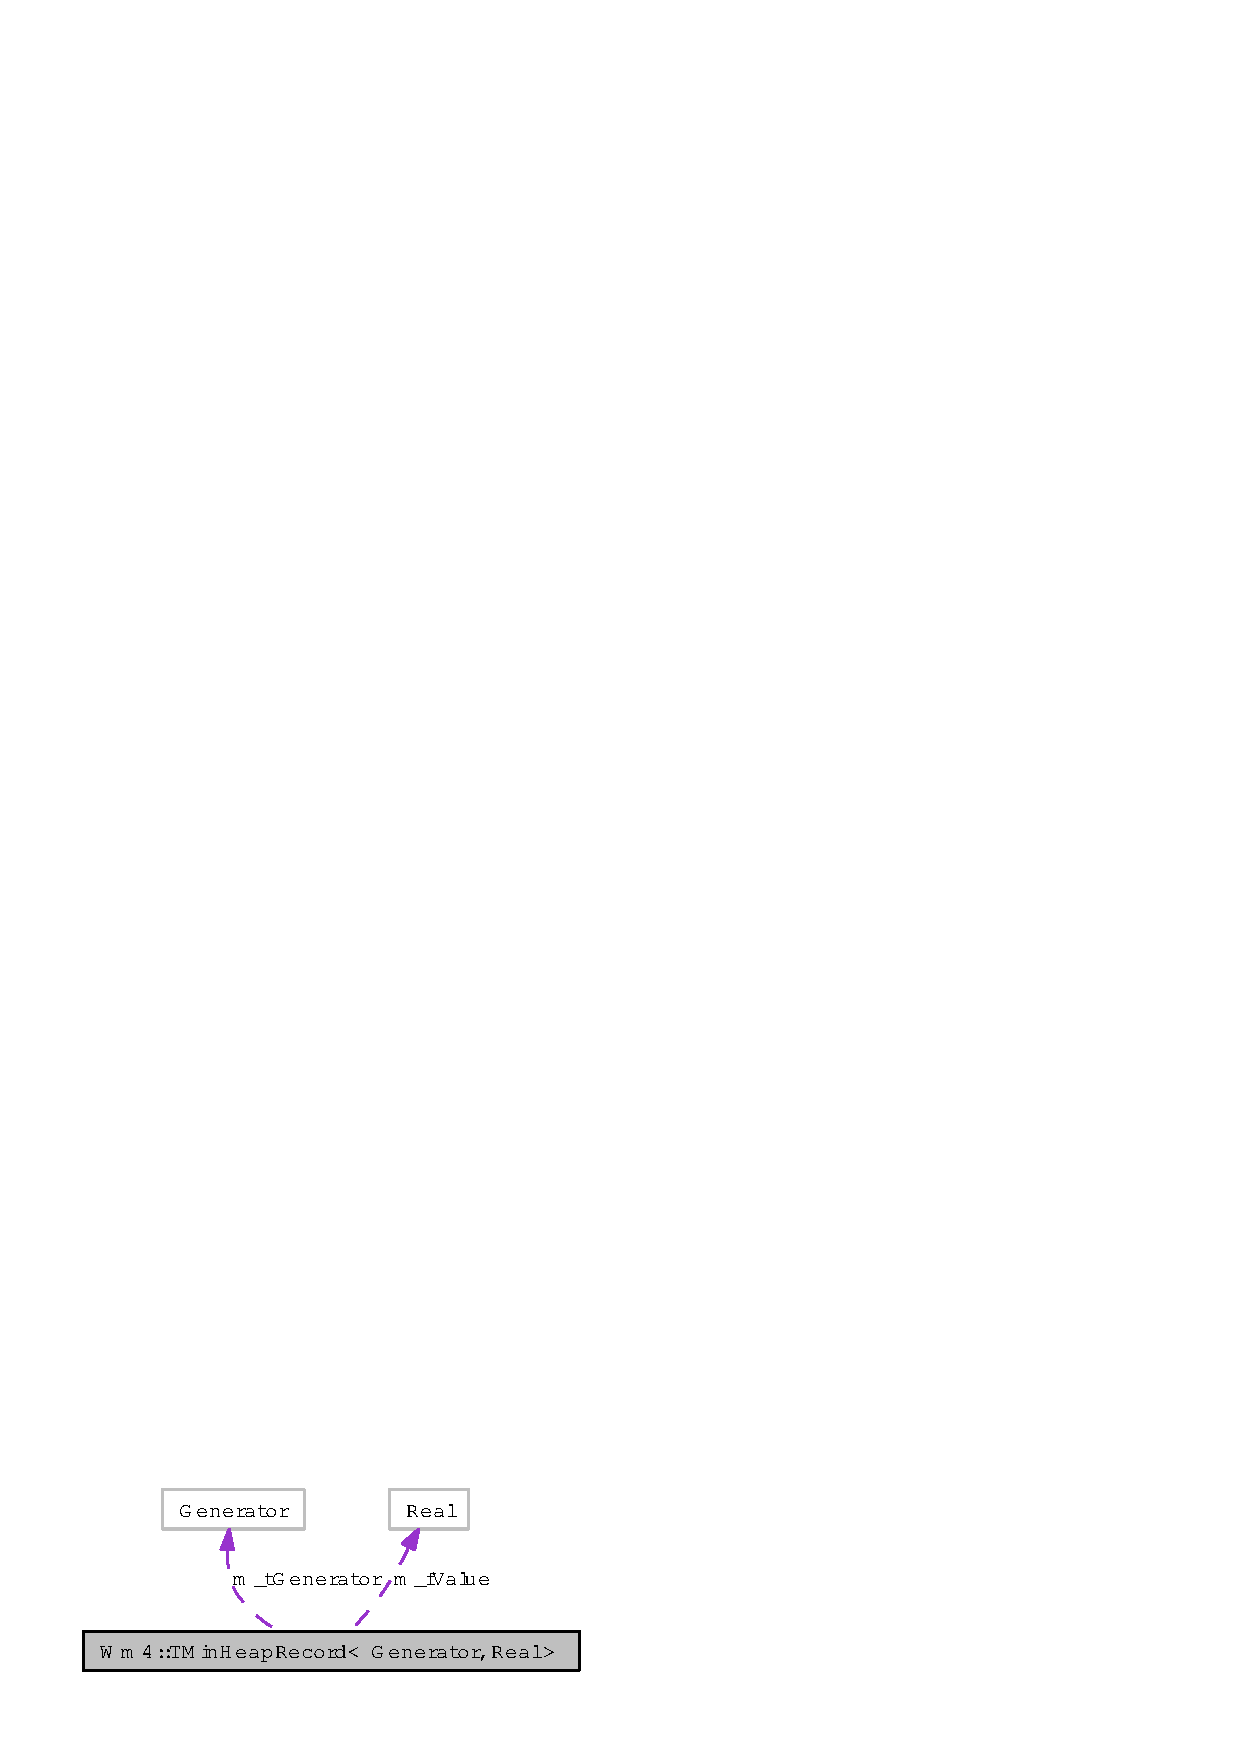
\includegraphics[width=141pt]{classWm4_1_1TMinHeapRecord__coll__graph}
\end{center}
\end{figure}
\subsection*{Public Member Functions}
\begin{CompactItemize}
\item 
{\bf TMin\-Heap\-Record} ()
\item 
{\bf $\sim$TMin\-Heap\-Record} ()
\item 
Generator {\bf Get\-Generator} () const
\item 
Real {\bf Get\-Value} () const
\end{CompactItemize}
\subsection*{Friends}
\begin{CompactItemize}
\item 
class {\bf TMin\-Heap$<$ Generator, Real $>$}
\end{CompactItemize}
\subsubsection*{template$<$typename Generator, typename Real$>$ class Wm4::TMin\-Heap\-Record$<$ Generator, Real $>$}



\subsection{Constructor \& Destructor Documentation}
\index{Wm4::TMinHeapRecord@{Wm4::TMin\-Heap\-Record}!TMinHeapRecord@{TMinHeapRecord}}
\index{TMinHeapRecord@{TMinHeapRecord}!Wm4::TMinHeapRecord@{Wm4::TMin\-Heap\-Record}}
\subsubsection{\setlength{\rightskip}{0pt plus 5cm}template$<$typename Generator, typename Real$>$ {\bf Wm4::TMin\-Heap\-Record}$<$ Generator, Real $>$::{\bf TMin\-Heap\-Record} ()}\label{classWm4_1_1TMinHeapRecord_768978badba3856ae212806b86c68345}


\index{Wm4::TMinHeapRecord@{Wm4::TMin\-Heap\-Record}!~TMinHeapRecord@{$\sim$TMinHeapRecord}}
\index{~TMinHeapRecord@{$\sim$TMinHeapRecord}!Wm4::TMinHeapRecord@{Wm4::TMin\-Heap\-Record}}
\subsubsection{\setlength{\rightskip}{0pt plus 5cm}template$<$typename Generator, typename Real$>$ {\bf Wm4::TMin\-Heap\-Record}$<$ Generator, Real $>$::$\sim${\bf TMin\-Heap\-Record} ()}\label{classWm4_1_1TMinHeapRecord_9b3f8321f3595b8f6d66ceeaf88154fb}




\subsection{Member Function Documentation}
\index{Wm4::TMinHeapRecord@{Wm4::TMin\-Heap\-Record}!GetGenerator@{GetGenerator}}
\index{GetGenerator@{GetGenerator}!Wm4::TMinHeapRecord@{Wm4::TMin\-Heap\-Record}}
\subsubsection{\setlength{\rightskip}{0pt plus 5cm}template$<$typename Generator, typename Real$>$ Generator {\bf Wm4::TMin\-Heap\-Record}$<$ Generator, Real $>$::Get\-Generator () const}\label{classWm4_1_1TMinHeapRecord_e93d74379d9efcd85430a2a1c959c86e}


\index{Wm4::TMinHeapRecord@{Wm4::TMin\-Heap\-Record}!GetValue@{GetValue}}
\index{GetValue@{GetValue}!Wm4::TMinHeapRecord@{Wm4::TMin\-Heap\-Record}}
\subsubsection{\setlength{\rightskip}{0pt plus 5cm}template$<$typename Generator, typename Real$>$ Real {\bf Wm4::TMin\-Heap\-Record}$<$ Generator, Real $>$::Get\-Value () const}\label{classWm4_1_1TMinHeapRecord_b10a9c41b2cf893521db8df9fedb5673}




\subsection{Friends And Related Function Documentation}
\index{Wm4::TMinHeapRecord@{Wm4::TMin\-Heap\-Record}!TMinHeap< Generator, Real >@{TMinHeap$<$ Generator, Real $>$}}
\index{TMinHeap< Generator, Real >@{TMinHeap$<$ Generator, Real $>$}!Wm4::TMinHeapRecord@{Wm4::TMin\-Heap\-Record}}
\subsubsection{\setlength{\rightskip}{0pt plus 5cm}template$<$typename Generator, typename Real$>$ friend class {\bf TMin\-Heap}$<$ Generator, Real $>$\hspace{0.3cm}{\tt  [friend]}}\label{classWm4_1_1TMinHeapRecord_54c578fd08bed627b76136aaae458026}




The documentation for this class was generated from the following file:\begin{CompactItemize}
\item 
{\bf Wm4TMin\-Heap.h}\end{CompactItemize}

\section{Wm4::TSmall\-Unordered\-Set$<$ T $>$ Class Template Reference}
\label{classWm4_1_1TSmallUnorderedSet}\index{Wm4::TSmallUnorderedSet@{Wm4::TSmallUnorderedSet}}
{\tt \#include $<$Wm4TSmall\-Unordered\-Set.h$>$}

Collaboration diagram for Wm4::TSmall\-Unordered\-Set$<$ T $>$:\begin{figure}[H]
\begin{center}
\leavevmode
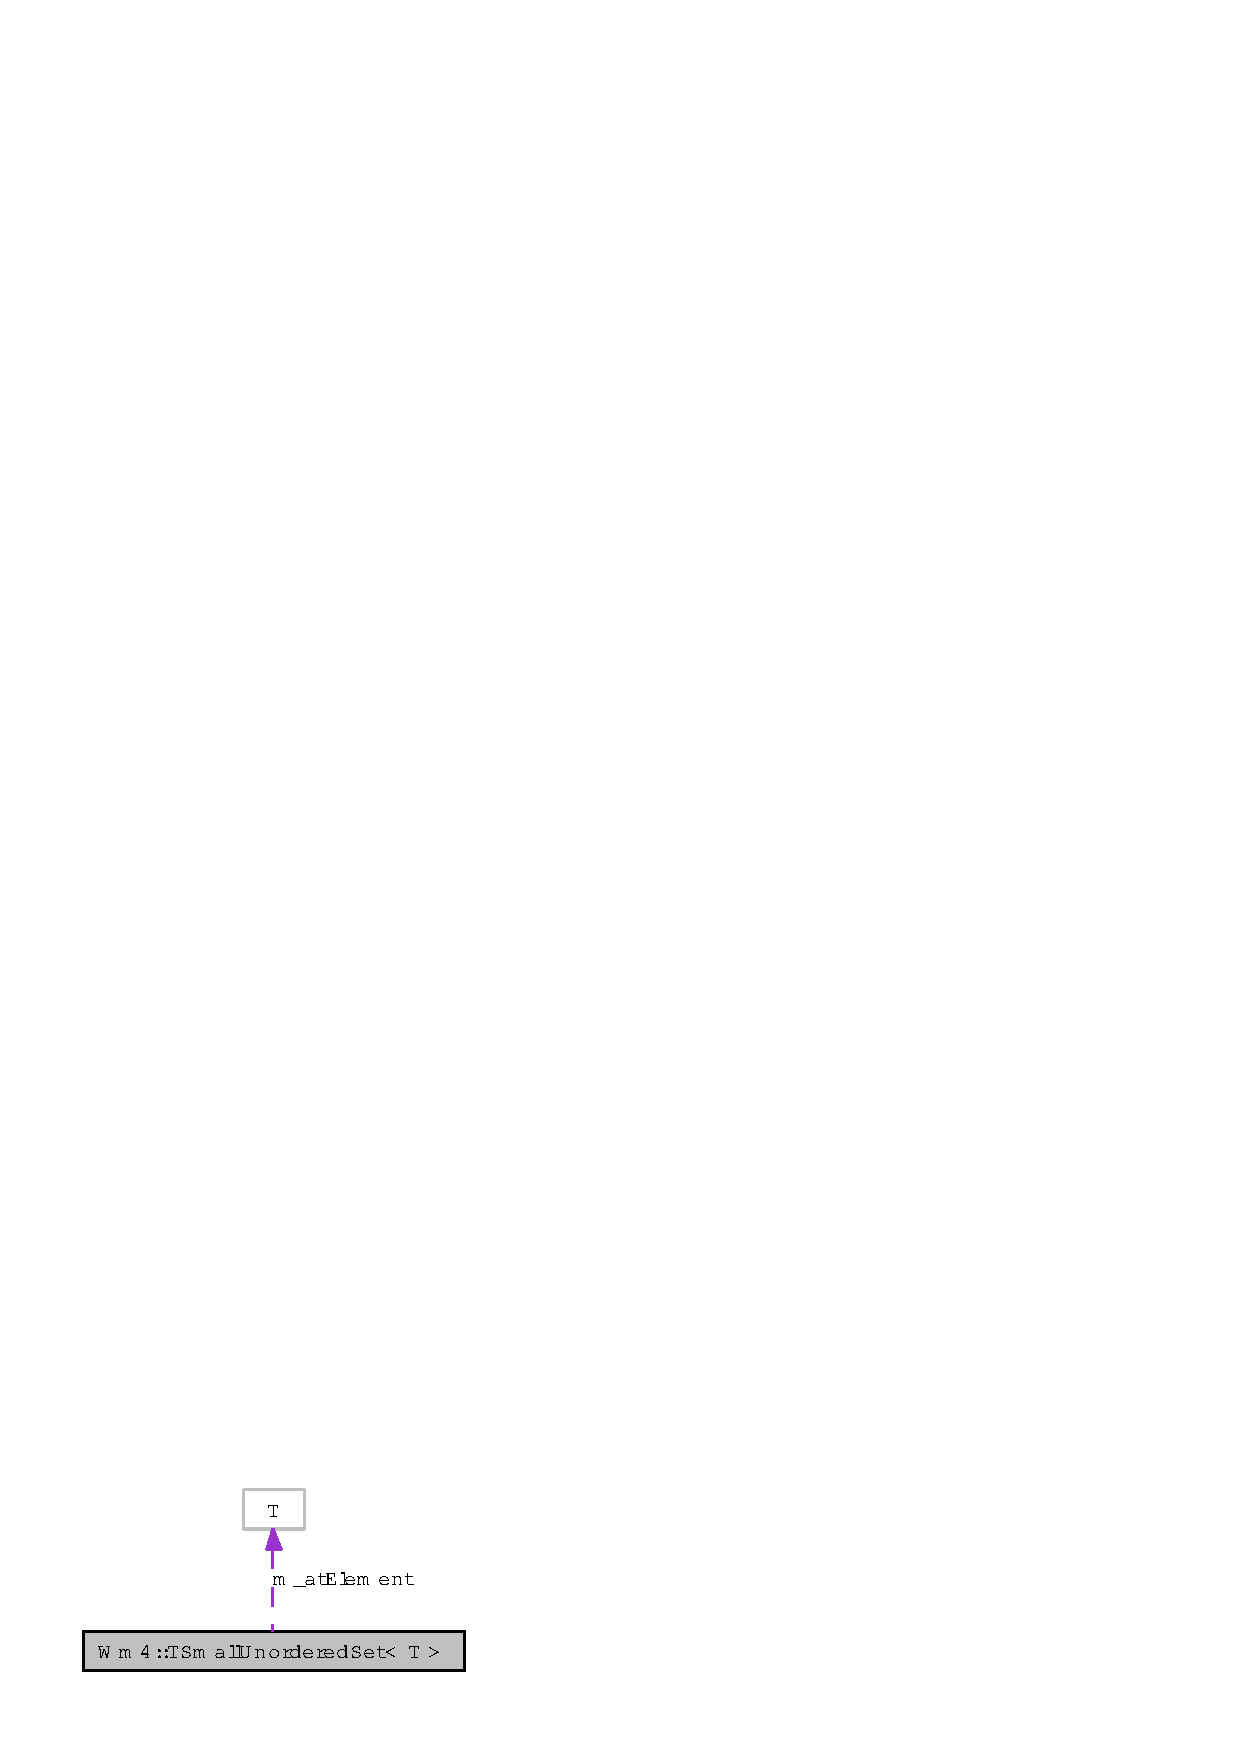
\includegraphics[width=113pt]{classWm4_1_1TSmallUnorderedSet__coll__graph}
\end{center}
\end{figure}
\subsection*{Public Member Functions}
\begin{CompactItemize}
\item 
{\bf TSmall\-Unordered\-Set} ()
\item 
{\bf TSmall\-Unordered\-Set} (int i\-Max\-Quantity, int i\-Grow\-By)
\item 
{\bf TSmall\-Unordered\-Set} (const {\bf TSmall\-Unordered\-Set} \&rk\-Set)
\item 
{\bf $\sim$TSmall\-Unordered\-Set} ()
\item 
{\bf TSmall\-Unordered\-Set} \& {\bf operator=} (const {\bf TSmall\-Unordered\-Set} \&rk\-Set)
\item 
int {\bf Get\-Max\-Quantity} () const
\item 
int {\bf Get\-Grow\-By} () const
\item 
int {\bf Get\-Quantity} () const
\item 
T $\ast$ {\bf Get\-Elements} ()
\item 
const T $\ast$ {\bf Get\-Elements} () const
\item 
T \& {\bf operator[$\,$]} (int i)
\item 
const T \& {\bf operator[$\,$]} (int i) const
\item 
bool {\bf Insert} (const T \&rk\-Element)
\item 
void {\bf Insert\-No\-Check} (const T \&rk\-Element)
\item 
bool {\bf Remove} (const T \&rk\-Element)
\item 
bool {\bf Exists} (const T \&rk\-Element)
\item 
void {\bf Clear} ()
\item 
void {\bf Clear} (int i\-Max\-Quantity, int i\-Grow\-By)
\end{CompactItemize}
\subsubsection*{template$<$class T$>$ class Wm4::TSmall\-Unordered\-Set$<$ T $>$}



\subsection{Constructor \& Destructor Documentation}
\index{Wm4::TSmallUnorderedSet@{Wm4::TSmall\-Unordered\-Set}!TSmallUnorderedSet@{TSmallUnorderedSet}}
\index{TSmallUnorderedSet@{TSmallUnorderedSet}!Wm4::TSmallUnorderedSet@{Wm4::TSmall\-Unordered\-Set}}
\subsubsection{\setlength{\rightskip}{0pt plus 5cm}template$<$class T$>$ {\bf Wm4::TSmall\-Unordered\-Set}$<$ T $>$::{\bf TSmall\-Unordered\-Set} ()}\label{classWm4_1_1TSmallUnorderedSet_2786e2c3052c7d03fded0338b7c4140b}


\index{Wm4::TSmallUnorderedSet@{Wm4::TSmall\-Unordered\-Set}!TSmallUnorderedSet@{TSmallUnorderedSet}}
\index{TSmallUnorderedSet@{TSmallUnorderedSet}!Wm4::TSmallUnorderedSet@{Wm4::TSmall\-Unordered\-Set}}
\subsubsection{\setlength{\rightskip}{0pt plus 5cm}template$<$class T$>$ {\bf Wm4::TSmall\-Unordered\-Set}$<$ T $>$::{\bf TSmall\-Unordered\-Set} (int {\em i\-Max\-Quantity}, int {\em i\-Grow\-By})}\label{classWm4_1_1TSmallUnorderedSet_bbde4fd2d9a7e5d80c9f05c25772a085}


\index{Wm4::TSmallUnorderedSet@{Wm4::TSmall\-Unordered\-Set}!TSmallUnorderedSet@{TSmallUnorderedSet}}
\index{TSmallUnorderedSet@{TSmallUnorderedSet}!Wm4::TSmallUnorderedSet@{Wm4::TSmall\-Unordered\-Set}}
\subsubsection{\setlength{\rightskip}{0pt plus 5cm}template$<$class T$>$ {\bf Wm4::TSmall\-Unordered\-Set}$<$ T $>$::{\bf TSmall\-Unordered\-Set} (const {\bf TSmall\-Unordered\-Set}$<$ T $>$ \& {\em rk\-Set})}\label{classWm4_1_1TSmallUnorderedSet_766b2da1ccddd2bd94928e4c09dc4332}


\index{Wm4::TSmallUnorderedSet@{Wm4::TSmall\-Unordered\-Set}!~TSmallUnorderedSet@{$\sim$TSmallUnorderedSet}}
\index{~TSmallUnorderedSet@{$\sim$TSmallUnorderedSet}!Wm4::TSmallUnorderedSet@{Wm4::TSmall\-Unordered\-Set}}
\subsubsection{\setlength{\rightskip}{0pt plus 5cm}template$<$class T$>$ {\bf Wm4::TSmall\-Unordered\-Set}$<$ T $>$::$\sim${\bf TSmall\-Unordered\-Set} ()}\label{classWm4_1_1TSmallUnorderedSet_8572c829ee007fa43a94c9dd0dd1be38}




\subsection{Member Function Documentation}
\index{Wm4::TSmallUnorderedSet@{Wm4::TSmall\-Unordered\-Set}!operator=@{operator=}}
\index{operator=@{operator=}!Wm4::TSmallUnorderedSet@{Wm4::TSmall\-Unordered\-Set}}
\subsubsection{\setlength{\rightskip}{0pt plus 5cm}template$<$class T$>$ {\bf TSmall\-Unordered\-Set}$<$ T $>$ \& {\bf Wm4::TSmall\-Unordered\-Set}$<$ T $>$::operator= (const {\bf TSmall\-Unordered\-Set}$<$ T $>$ \& {\em rk\-Set})}\label{classWm4_1_1TSmallUnorderedSet_6119f459d34f6edcb9a29c84aa225ae4}


\index{Wm4::TSmallUnorderedSet@{Wm4::TSmall\-Unordered\-Set}!GetMaxQuantity@{GetMaxQuantity}}
\index{GetMaxQuantity@{GetMaxQuantity}!Wm4::TSmallUnorderedSet@{Wm4::TSmall\-Unordered\-Set}}
\subsubsection{\setlength{\rightskip}{0pt plus 5cm}template$<$class T$>$ int {\bf Wm4::TSmall\-Unordered\-Set}$<$ T $>$::Get\-Max\-Quantity () const}\label{classWm4_1_1TSmallUnorderedSet_281c207a10abb8c7c1586ee40c353cd4}


\index{Wm4::TSmallUnorderedSet@{Wm4::TSmall\-Unordered\-Set}!GetGrowBy@{GetGrowBy}}
\index{GetGrowBy@{GetGrowBy}!Wm4::TSmallUnorderedSet@{Wm4::TSmall\-Unordered\-Set}}
\subsubsection{\setlength{\rightskip}{0pt plus 5cm}template$<$class T$>$ int {\bf Wm4::TSmall\-Unordered\-Set}$<$ T $>$::Get\-Grow\-By () const}\label{classWm4_1_1TSmallUnorderedSet_f2c717eeb8fb35f11579611870adfe92}


\index{Wm4::TSmallUnorderedSet@{Wm4::TSmall\-Unordered\-Set}!GetQuantity@{GetQuantity}}
\index{GetQuantity@{GetQuantity}!Wm4::TSmallUnorderedSet@{Wm4::TSmall\-Unordered\-Set}}
\subsubsection{\setlength{\rightskip}{0pt plus 5cm}template$<$class T$>$ int {\bf Wm4::TSmall\-Unordered\-Set}$<$ T $>$::Get\-Quantity () const}\label{classWm4_1_1TSmallUnorderedSet_22646babffba340ed45d1a0823333616}


\index{Wm4::TSmallUnorderedSet@{Wm4::TSmall\-Unordered\-Set}!GetElements@{GetElements}}
\index{GetElements@{GetElements}!Wm4::TSmallUnorderedSet@{Wm4::TSmall\-Unordered\-Set}}
\subsubsection{\setlength{\rightskip}{0pt plus 5cm}template$<$class T$>$ T $\ast$ {\bf Wm4::TSmall\-Unordered\-Set}$<$ T $>$::Get\-Elements ()}\label{classWm4_1_1TSmallUnorderedSet_ac98e31842f3cdbe7331663d969bf969}


\index{Wm4::TSmallUnorderedSet@{Wm4::TSmall\-Unordered\-Set}!GetElements@{GetElements}}
\index{GetElements@{GetElements}!Wm4::TSmallUnorderedSet@{Wm4::TSmall\-Unordered\-Set}}
\subsubsection{\setlength{\rightskip}{0pt plus 5cm}template$<$class T$>$ const T $\ast$ {\bf Wm4::TSmall\-Unordered\-Set}$<$ T $>$::Get\-Elements () const}\label{classWm4_1_1TSmallUnorderedSet_ea47a8d4ea1f56c0b5be02648e5f2014}


\index{Wm4::TSmallUnorderedSet@{Wm4::TSmall\-Unordered\-Set}!operator[]@{operator[]}}
\index{operator[]@{operator[]}!Wm4::TSmallUnorderedSet@{Wm4::TSmall\-Unordered\-Set}}
\subsubsection{\setlength{\rightskip}{0pt plus 5cm}template$<$class T$>$ T \& {\bf Wm4::TSmall\-Unordered\-Set}$<$ T $>$::operator[$\,$] (int {\em i})}\label{classWm4_1_1TSmallUnorderedSet_9b16af01eac1f26d3e28e896d67cc1f3}


\index{Wm4::TSmallUnorderedSet@{Wm4::TSmall\-Unordered\-Set}!operator[]@{operator[]}}
\index{operator[]@{operator[]}!Wm4::TSmallUnorderedSet@{Wm4::TSmall\-Unordered\-Set}}
\subsubsection{\setlength{\rightskip}{0pt plus 5cm}template$<$class T$>$ const T \& {\bf Wm4::TSmall\-Unordered\-Set}$<$ T $>$::operator[$\,$] (int {\em i}) const}\label{classWm4_1_1TSmallUnorderedSet_c251450549fb315ae85b93ed12fceec0}


\index{Wm4::TSmallUnorderedSet@{Wm4::TSmall\-Unordered\-Set}!Insert@{Insert}}
\index{Insert@{Insert}!Wm4::TSmallUnorderedSet@{Wm4::TSmall\-Unordered\-Set}}
\subsubsection{\setlength{\rightskip}{0pt plus 5cm}template$<$class T$>$ bool {\bf Wm4::TSmall\-Unordered\-Set}$<$ T $>$::Insert (const T \& {\em rk\-Element})}\label{classWm4_1_1TSmallUnorderedSet_9262b59b145e28cebe4d4acfdfe7c6ad}


\index{Wm4::TSmallUnorderedSet@{Wm4::TSmall\-Unordered\-Set}!InsertNoCheck@{InsertNoCheck}}
\index{InsertNoCheck@{InsertNoCheck}!Wm4::TSmallUnorderedSet@{Wm4::TSmall\-Unordered\-Set}}
\subsubsection{\setlength{\rightskip}{0pt plus 5cm}template$<$class T$>$ void {\bf Wm4::TSmall\-Unordered\-Set}$<$ T $>$::Insert\-No\-Check (const T \& {\em rk\-Element})}\label{classWm4_1_1TSmallUnorderedSet_c60d4e8f2ccff74c6ea026496de874bc}


\index{Wm4::TSmallUnorderedSet@{Wm4::TSmall\-Unordered\-Set}!Remove@{Remove}}
\index{Remove@{Remove}!Wm4::TSmallUnorderedSet@{Wm4::TSmall\-Unordered\-Set}}
\subsubsection{\setlength{\rightskip}{0pt plus 5cm}template$<$class T$>$ bool {\bf Wm4::TSmall\-Unordered\-Set}$<$ T $>$::Remove (const T \& {\em rk\-Element})}\label{classWm4_1_1TSmallUnorderedSet_213b21afb81bb1a41b915870ad7d5962}


\index{Wm4::TSmallUnorderedSet@{Wm4::TSmall\-Unordered\-Set}!Exists@{Exists}}
\index{Exists@{Exists}!Wm4::TSmallUnorderedSet@{Wm4::TSmall\-Unordered\-Set}}
\subsubsection{\setlength{\rightskip}{0pt plus 5cm}template$<$class T$>$ bool {\bf Wm4::TSmall\-Unordered\-Set}$<$ T $>$::Exists (const T \& {\em rk\-Element})}\label{classWm4_1_1TSmallUnorderedSet_e2fc96cf61aaadf6815e0245120d8dd4}


\index{Wm4::TSmallUnorderedSet@{Wm4::TSmall\-Unordered\-Set}!Clear@{Clear}}
\index{Clear@{Clear}!Wm4::TSmallUnorderedSet@{Wm4::TSmall\-Unordered\-Set}}
\subsubsection{\setlength{\rightskip}{0pt plus 5cm}template$<$class T$>$ void {\bf Wm4::TSmall\-Unordered\-Set}$<$ T $>$::Clear ()}\label{classWm4_1_1TSmallUnorderedSet_5355d2d639759b9b9e4d766beab04b21}


\index{Wm4::TSmallUnorderedSet@{Wm4::TSmall\-Unordered\-Set}!Clear@{Clear}}
\index{Clear@{Clear}!Wm4::TSmallUnorderedSet@{Wm4::TSmall\-Unordered\-Set}}
\subsubsection{\setlength{\rightskip}{0pt plus 5cm}template$<$class T$>$ void {\bf Wm4::TSmall\-Unordered\-Set}$<$ T $>$::Clear (int {\em i\-Max\-Quantity}, int {\em i\-Grow\-By})}\label{classWm4_1_1TSmallUnorderedSet_a041a9c43cef7aa6e765c9d15824982d}




The documentation for this class was generated from the following file:\begin{CompactItemize}
\item 
{\bf Wm4TSmall\-Unordered\-Set.h}\end{CompactItemize}

\section{Wm4::TString\-Hash\-Table$<$ TVALUE $>$ Class Template Reference}
\label{classWm4_1_1TStringHashTable}\index{Wm4::TStringHashTable@{Wm4::TStringHashTable}}
{\tt \#include $<$Wm4TString\-Hash\-Table.h$>$}

\subsection*{Public Member Functions}
\begin{CompactItemize}
\item 
{\bf TString\-Hash\-Table} (int i\-Table\-Size)
\item 
{\bf $\sim$TString\-Hash\-Table} ()
\item 
int {\bf Get\-Quantity} () const
\item 
bool {\bf Insert} (const std::string \&rk\-Key, const TVALUE \&rt\-Value)
\item 
TVALUE $\ast$ {\bf Find} (const std::string \&rk\-Key) const
\item 
bool {\bf Remove} (const std::string \&rk\-Key)
\item 
void {\bf Remove\-All} ()
\item 
TVALUE $\ast$ {\bf Get\-First} (std::string $\ast$pk\-Key) const
\item 
TVALUE $\ast$ {\bf Get\-Next} (std::string $\ast$pk\-Key) const
\end{CompactItemize}
\subsection*{Classes}
\begin{CompactItemize}
\item 
class \textbf{Hash\-Item}
\end{CompactItemize}
\subsubsection*{template$<$class TVALUE$>$ class Wm4::TString\-Hash\-Table$<$ TVALUE $>$}



\subsection{Constructor \& Destructor Documentation}
\index{Wm4::TStringHashTable@{Wm4::TString\-Hash\-Table}!TStringHashTable@{TStringHashTable}}
\index{TStringHashTable@{TStringHashTable}!Wm4::TStringHashTable@{Wm4::TString\-Hash\-Table}}
\subsubsection{\setlength{\rightskip}{0pt plus 5cm}template$<$class TVALUE$>$ {\bf Wm4::TString\-Hash\-Table}$<$ TVALUE $>$::{\bf TString\-Hash\-Table} (int {\em i\-Table\-Size})}\label{classWm4_1_1TStringHashTable_2f8e9f17a649a3e9c38f388cdca6e012}


\index{Wm4::TStringHashTable@{Wm4::TString\-Hash\-Table}!~TStringHashTable@{$\sim$TStringHashTable}}
\index{~TStringHashTable@{$\sim$TStringHashTable}!Wm4::TStringHashTable@{Wm4::TString\-Hash\-Table}}
\subsubsection{\setlength{\rightskip}{0pt plus 5cm}template$<$class TVALUE$>$ {\bf Wm4::TString\-Hash\-Table}$<$ TVALUE $>$::$\sim${\bf TString\-Hash\-Table} ()}\label{classWm4_1_1TStringHashTable_9728e8c60fdea12a8c9b7ed9b4204f43}




\subsection{Member Function Documentation}
\index{Wm4::TStringHashTable@{Wm4::TString\-Hash\-Table}!GetQuantity@{GetQuantity}}
\index{GetQuantity@{GetQuantity}!Wm4::TStringHashTable@{Wm4::TString\-Hash\-Table}}
\subsubsection{\setlength{\rightskip}{0pt plus 5cm}template$<$class TVALUE$>$ int {\bf Wm4::TString\-Hash\-Table}$<$ TVALUE $>$::Get\-Quantity () const}\label{classWm4_1_1TStringHashTable_59651403a906cca5c0aa7d19a471ae82}


\index{Wm4::TStringHashTable@{Wm4::TString\-Hash\-Table}!Insert@{Insert}}
\index{Insert@{Insert}!Wm4::TStringHashTable@{Wm4::TString\-Hash\-Table}}
\subsubsection{\setlength{\rightskip}{0pt plus 5cm}template$<$class TVALUE$>$ bool {\bf Wm4::TString\-Hash\-Table}$<$ TVALUE $>$::Insert (const std::string \& {\em rk\-Key}, const TVALUE \& {\em rt\-Value})}\label{classWm4_1_1TStringHashTable_b9c25ff9e818e32693f5e7eb16cbedd9}


\index{Wm4::TStringHashTable@{Wm4::TString\-Hash\-Table}!Find@{Find}}
\index{Find@{Find}!Wm4::TStringHashTable@{Wm4::TString\-Hash\-Table}}
\subsubsection{\setlength{\rightskip}{0pt plus 5cm}template$<$class TVALUE$>$ TVALUE $\ast$ {\bf Wm4::TString\-Hash\-Table}$<$ TVALUE $>$::Find (const std::string \& {\em rk\-Key}) const}\label{classWm4_1_1TStringHashTable_0655fe1516c18976e0d260cfdbad3db7}


\index{Wm4::TStringHashTable@{Wm4::TString\-Hash\-Table}!Remove@{Remove}}
\index{Remove@{Remove}!Wm4::TStringHashTable@{Wm4::TString\-Hash\-Table}}
\subsubsection{\setlength{\rightskip}{0pt plus 5cm}template$<$class TVALUE$>$ bool {\bf Wm4::TString\-Hash\-Table}$<$ TVALUE $>$::Remove (const std::string \& {\em rk\-Key})}\label{classWm4_1_1TStringHashTable_7c4c6b2071b30bae479c18a8eaf721dd}


\index{Wm4::TStringHashTable@{Wm4::TString\-Hash\-Table}!RemoveAll@{RemoveAll}}
\index{RemoveAll@{RemoveAll}!Wm4::TStringHashTable@{Wm4::TString\-Hash\-Table}}
\subsubsection{\setlength{\rightskip}{0pt plus 5cm}template$<$class TVALUE$>$ void {\bf Wm4::TString\-Hash\-Table}$<$ TVALUE $>$::Remove\-All ()}\label{classWm4_1_1TStringHashTable_654fcff20a8e68aa8c2c14577b0c11b4}


\index{Wm4::TStringHashTable@{Wm4::TString\-Hash\-Table}!GetFirst@{GetFirst}}
\index{GetFirst@{GetFirst}!Wm4::TStringHashTable@{Wm4::TString\-Hash\-Table}}
\subsubsection{\setlength{\rightskip}{0pt plus 5cm}template$<$class TVALUE$>$ TVALUE $\ast$ {\bf Wm4::TString\-Hash\-Table}$<$ TVALUE $>$::Get\-First (std::string $\ast$ {\em pk\-Key}) const}\label{classWm4_1_1TStringHashTable_728f59068296861d743449d8d357768f}


\index{Wm4::TStringHashTable@{Wm4::TString\-Hash\-Table}!GetNext@{GetNext}}
\index{GetNext@{GetNext}!Wm4::TStringHashTable@{Wm4::TString\-Hash\-Table}}
\subsubsection{\setlength{\rightskip}{0pt plus 5cm}template$<$class TVALUE$>$ TVALUE $\ast$ {\bf Wm4::TString\-Hash\-Table}$<$ TVALUE $>$::Get\-Next (std::string $\ast$ {\em pk\-Key}) const}\label{classWm4_1_1TStringHashTable_0d203a2bd2cdb9fc6189d81d96d73aa2}




The documentation for this class was generated from the following file:\begin{CompactItemize}
\item 
{\bf Wm4TString\-Hash\-Table.h}\end{CompactItemize}

\section{Wm4::TTuple$<$ DIMENSION, TYPE $>$ Class Template Reference}
\label{classWm4_1_1TTuple}\index{Wm4::TTuple@{Wm4::TTuple}}
{\tt \#include $<$Wm4TTuple.h$>$}

Collaboration diagram for Wm4::TTuple$<$ DIMENSION, TYPE $>$:\begin{figure}[H]
\begin{center}
\leavevmode
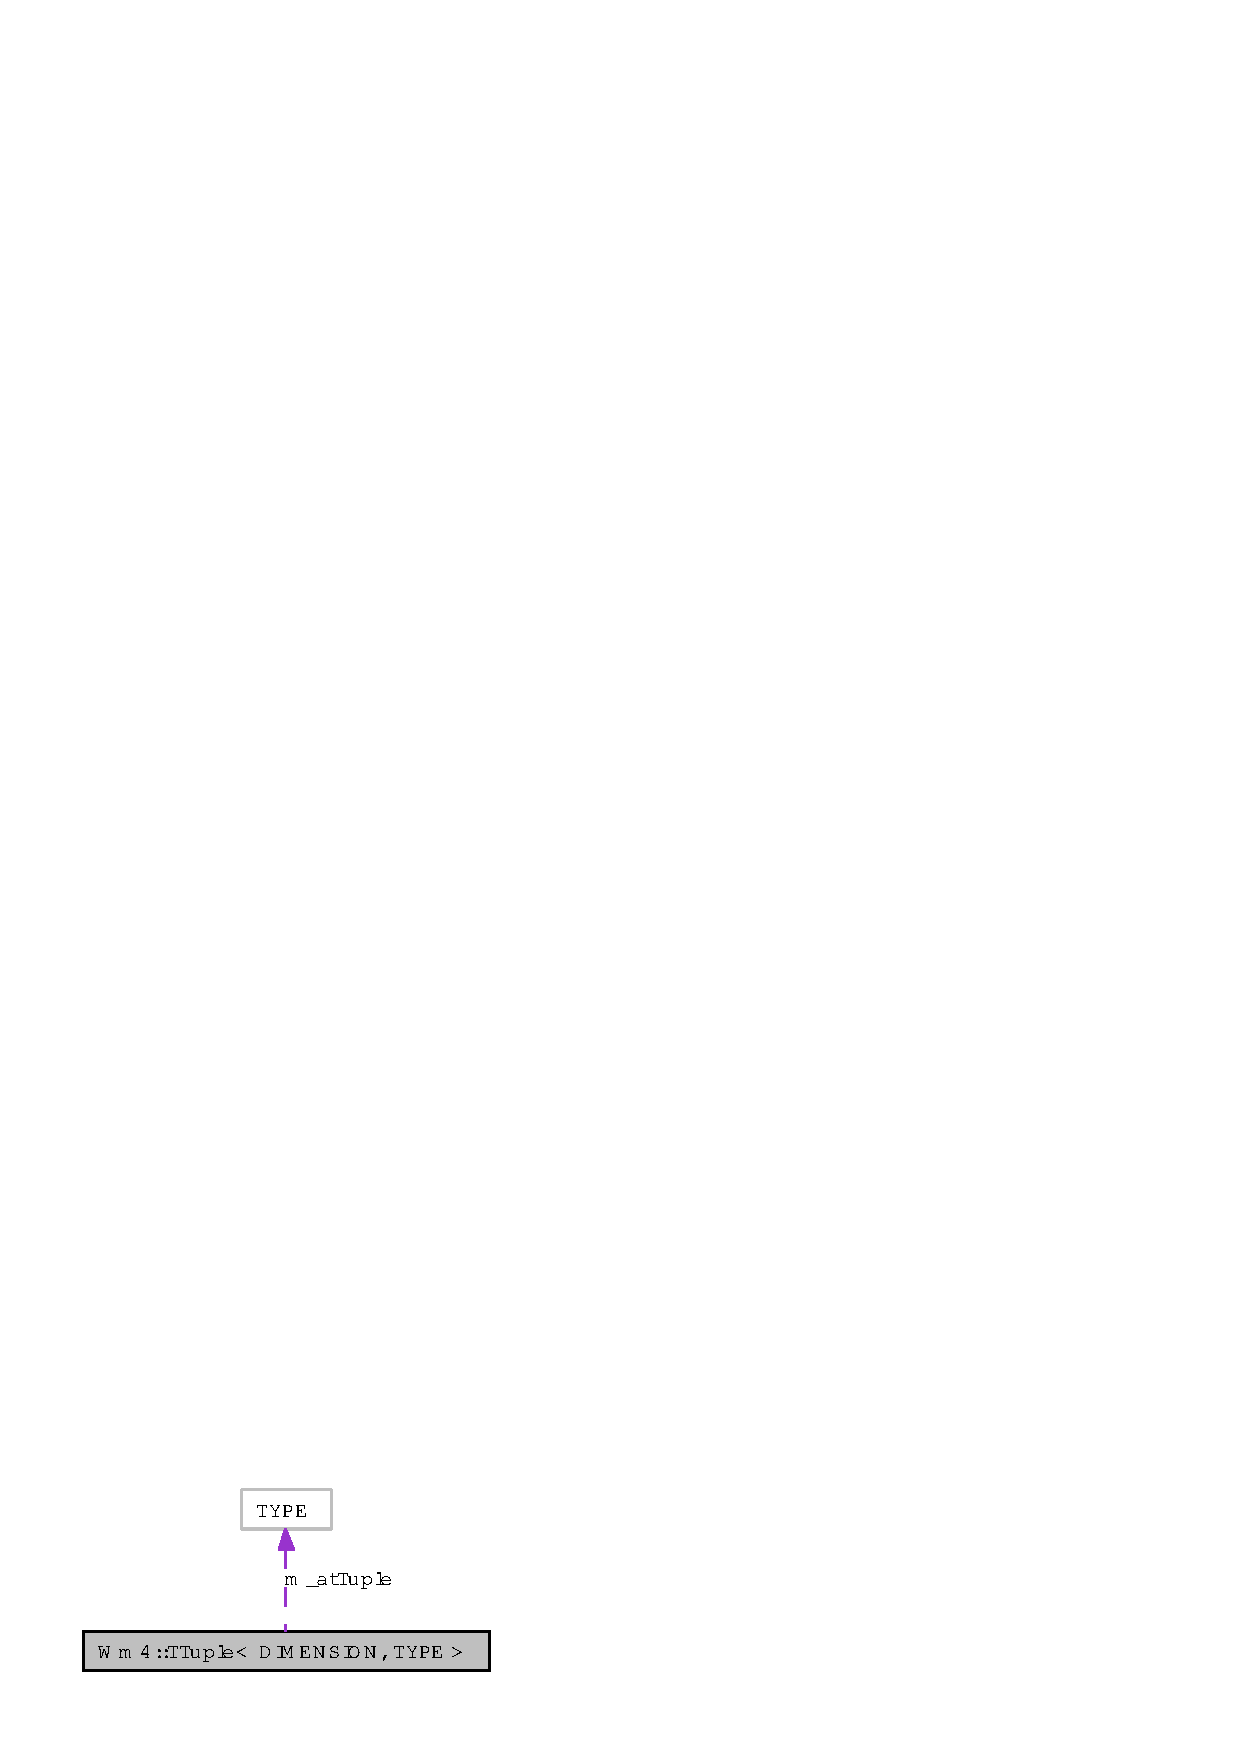
\includegraphics[width=119pt]{classWm4_1_1TTuple__coll__graph}
\end{center}
\end{figure}
\subsection*{Public Member Functions}
\begin{CompactItemize}
\item 
{\bf TTuple} ()
\item 
{\bf TTuple} (const {\bf TTuple} \&rk\-T)
\item 
{\bf $\sim$TTuple} ()
\item 
{\bf operator const TYPE $\ast$} () const
\item 
{\bf operator TYPE $\ast$} ()
\item 
TYPE {\bf operator[$\,$]} (int i) const
\item 
TYPE \& {\bf operator[$\,$]} (int i)
\item 
{\bf TTuple} \& {\bf operator=} (const {\bf TTuple} \&rk\-T)
\item 
bool {\bf operator==} (const {\bf TTuple} \&rk\-T) const
\item 
bool {\bf operator!=} (const {\bf TTuple} \&rk\-T) const
\item 
bool {\bf operator$<$} (const {\bf TTuple} \&rk\-T) const
\item 
bool {\bf operator$<$=} (const {\bf TTuple} \&rk\-T) const
\item 
bool {\bf operator$>$} (const {\bf TTuple} \&rk\-T) const
\item 
bool {\bf operator$>$=} (const {\bf TTuple} \&rk\-T) const
\end{CompactItemize}
\subsubsection*{template$<$int DIMENSION, class TYPE$>$ class Wm4::TTuple$<$ DIMENSION, TYPE $>$}



\subsection{Constructor \& Destructor Documentation}
\index{Wm4::TTuple@{Wm4::TTuple}!TTuple@{TTuple}}
\index{TTuple@{TTuple}!Wm4::TTuple@{Wm4::TTuple}}
\subsubsection{\setlength{\rightskip}{0pt plus 5cm}template$<$int DIMENSION, class TYPE$>$ {\bf Wm4::TTuple}$<$ DIMENSION, TYPE $>$::{\bf TTuple} ()}\label{classWm4_1_1TTuple_5b043df7abee10c61293ca045af3b261}


\index{Wm4::TTuple@{Wm4::TTuple}!TTuple@{TTuple}}
\index{TTuple@{TTuple}!Wm4::TTuple@{Wm4::TTuple}}
\subsubsection{\setlength{\rightskip}{0pt plus 5cm}template$<$int DIMENSION, class TYPE$>$ {\bf Wm4::TTuple}$<$ DIMENSION, TYPE $>$::{\bf TTuple} (const {\bf TTuple}$<$ DIMENSION, TYPE $>$ \& {\em rk\-T})}\label{classWm4_1_1TTuple_560aa4608ca020c6e4cfb909230a5b71}


\index{Wm4::TTuple@{Wm4::TTuple}!~TTuple@{$\sim$TTuple}}
\index{~TTuple@{$\sim$TTuple}!Wm4::TTuple@{Wm4::TTuple}}
\subsubsection{\setlength{\rightskip}{0pt plus 5cm}template$<$int DIMENSION, class TYPE$>$ {\bf Wm4::TTuple}$<$ DIMENSION, TYPE $>$::$\sim${\bf TTuple} ()}\label{classWm4_1_1TTuple_d159f7bcd3df93b7699bc1fc9f827dd7}




\subsection{Member Function Documentation}
\index{Wm4::TTuple@{Wm4::TTuple}!operator const TYPE *@{operator const TYPE $\ast$}}
\index{operator const TYPE *@{operator const TYPE $\ast$}!Wm4::TTuple@{Wm4::TTuple}}
\subsubsection{\setlength{\rightskip}{0pt plus 5cm}template$<$int DIMENSION, class TYPE$>$ {\bf Wm4::TTuple}$<$ DIMENSION, TYPE $>$::operator const TYPE $\ast$ () const}\label{classWm4_1_1TTuple_2d99c029fedc1bb4d195507861930c11}


\index{Wm4::TTuple@{Wm4::TTuple}!operator TYPE *@{operator TYPE $\ast$}}
\index{operator TYPE *@{operator TYPE $\ast$}!Wm4::TTuple@{Wm4::TTuple}}
\subsubsection{\setlength{\rightskip}{0pt plus 5cm}template$<$int DIMENSION, class TYPE$>$ {\bf Wm4::TTuple}$<$ DIMENSION, TYPE $>$::operator TYPE $\ast$ ()}\label{classWm4_1_1TTuple_ac311c3da5d2fcc9fa6c0cf2c796cda3}


\index{Wm4::TTuple@{Wm4::TTuple}!operator[]@{operator[]}}
\index{operator[]@{operator[]}!Wm4::TTuple@{Wm4::TTuple}}
\subsubsection{\setlength{\rightskip}{0pt plus 5cm}template$<$int DIMENSION, class TYPE$>$ TYPE {\bf Wm4::TTuple}$<$ DIMENSION, TYPE $>$::operator[$\,$] (int {\em i}) const}\label{classWm4_1_1TTuple_f51bf23c29d7df64d4c72e3105a9414f}


\index{Wm4::TTuple@{Wm4::TTuple}!operator[]@{operator[]}}
\index{operator[]@{operator[]}!Wm4::TTuple@{Wm4::TTuple}}
\subsubsection{\setlength{\rightskip}{0pt plus 5cm}template$<$int DIMENSION, class TYPE$>$ TYPE \& {\bf Wm4::TTuple}$<$ DIMENSION, TYPE $>$::operator[$\,$] (int {\em i})}\label{classWm4_1_1TTuple_6ea2360a9c9de80d04d739cd9dde420e}


\index{Wm4::TTuple@{Wm4::TTuple}!operator=@{operator=}}
\index{operator=@{operator=}!Wm4::TTuple@{Wm4::TTuple}}
\subsubsection{\setlength{\rightskip}{0pt plus 5cm}template$<$int DIMENSION, class TYPE$>$ {\bf TTuple}$<$ DIMENSION, TYPE $>$ \& {\bf Wm4::TTuple}$<$ DIMENSION, TYPE $>$::operator= (const {\bf TTuple}$<$ DIMENSION, TYPE $>$ \& {\em rk\-T})}\label{classWm4_1_1TTuple_5ce1feaa5ac7e0acde60c29563abd980}


\index{Wm4::TTuple@{Wm4::TTuple}!operator==@{operator==}}
\index{operator==@{operator==}!Wm4::TTuple@{Wm4::TTuple}}
\subsubsection{\setlength{\rightskip}{0pt plus 5cm}template$<$int DIMENSION, class TYPE$>$ bool {\bf Wm4::TTuple}$<$ DIMENSION, TYPE $>$::operator== (const {\bf TTuple}$<$ DIMENSION, TYPE $>$ \& {\em rk\-T}) const}\label{classWm4_1_1TTuple_31b88cc79b1f75b96b9997f22148abf7}


\index{Wm4::TTuple@{Wm4::TTuple}!operator"!=@{operator"!=}}
\index{operator"!=@{operator"!=}!Wm4::TTuple@{Wm4::TTuple}}
\subsubsection{\setlength{\rightskip}{0pt plus 5cm}template$<$int DIMENSION, class TYPE$>$ bool {\bf Wm4::TTuple}$<$ DIMENSION, TYPE $>$::operator!= (const {\bf TTuple}$<$ DIMENSION, TYPE $>$ \& {\em rk\-T}) const}\label{classWm4_1_1TTuple_1c0a98b2e5a44e2d6ed7fa51de8381af}


\index{Wm4::TTuple@{Wm4::TTuple}!operator<@{operator$<$}}
\index{operator<@{operator$<$}!Wm4::TTuple@{Wm4::TTuple}}
\subsubsection{\setlength{\rightskip}{0pt plus 5cm}template$<$int DIMENSION, class TYPE$>$ bool {\bf Wm4::TTuple}$<$ DIMENSION, TYPE $>$::operator$<$ (const {\bf TTuple}$<$ DIMENSION, TYPE $>$ \& {\em rk\-T}) const}\label{classWm4_1_1TTuple_9fbc4e18f280382e7107140697bb9025}


\index{Wm4::TTuple@{Wm4::TTuple}!operator<=@{operator$<$=}}
\index{operator<=@{operator$<$=}!Wm4::TTuple@{Wm4::TTuple}}
\subsubsection{\setlength{\rightskip}{0pt plus 5cm}template$<$int DIMENSION, class TYPE$>$ bool {\bf Wm4::TTuple}$<$ DIMENSION, TYPE $>$::operator$<$= (const {\bf TTuple}$<$ DIMENSION, TYPE $>$ \& {\em rk\-T}) const}\label{classWm4_1_1TTuple_86419d1d2e2fceacc6b47beae87f3919}


\index{Wm4::TTuple@{Wm4::TTuple}!operator>@{operator$>$}}
\index{operator>@{operator$>$}!Wm4::TTuple@{Wm4::TTuple}}
\subsubsection{\setlength{\rightskip}{0pt plus 5cm}template$<$int DIMENSION, class TYPE$>$ bool {\bf Wm4::TTuple}$<$ DIMENSION, TYPE $>$::operator$>$ (const {\bf TTuple}$<$ DIMENSION, TYPE $>$ \& {\em rk\-T}) const}\label{classWm4_1_1TTuple_0242a0b4520f71efc7019f0f4be11962}


\index{Wm4::TTuple@{Wm4::TTuple}!operator>=@{operator$>$=}}
\index{operator>=@{operator$>$=}!Wm4::TTuple@{Wm4::TTuple}}
\subsubsection{\setlength{\rightskip}{0pt plus 5cm}template$<$int DIMENSION, class TYPE$>$ bool {\bf Wm4::TTuple}$<$ DIMENSION, TYPE $>$::operator$>$= (const {\bf TTuple}$<$ DIMENSION, TYPE $>$ \& {\em rk\-T}) const}\label{classWm4_1_1TTuple_2c95a38aa11afcc29f7bbc94c20de9e1}




The documentation for this class was generated from the following file:\begin{CompactItemize}
\item 
{\bf Wm4TTuple.h}\end{CompactItemize}

\section{v\_\-hash Struct Reference}
\label{structv__hash}\index{v_hash@{v\_\-hash}}
{\tt \#include $<$meshmorph.h$>$}

\subsection*{Public Member Functions}
\begin{CompactItemize}
\item 
{\bf u4} {\bf operator()} ({\bf Vertex} $\ast$i) const
\end{CompactItemize}


\subsection{Member Function Documentation}
\index{v_hash@{v\_\-hash}!operator()@{operator()}}
\index{operator()@{operator()}!v_hash@{v\_\-hash}}
\subsubsection{\setlength{\rightskip}{0pt plus 5cm}{\bf u4} v\_\-hash::operator() ({\bf Vertex} $\ast$ {\em i}) const\hspace{0.3cm}{\tt  [inline]}}\label{structv__hash_70a95c1d9155c62221449480fd43bef8}




The documentation for this struct was generated from the following file:\begin{CompactItemize}
\item 
{\bf meshmorph.h}\end{CompactItemize}

\section{vector3 Struct Reference}
\label{structvector3}\index{vector3@{vector3}}
{\tt \#include $<$meshmorph.h$>$}

\subsection*{Public Member Functions}
\begin{CompactItemize}
\item 
{\bf vector3} (void)
\item 
{\bf vector3} (double x, double y, double z)
\item 
{\bf vector3} \& {\bf operator=} (const {\bf vector3} \&v)
\item 
{\bf vector3} \& {\bf operator+=} (double a)
\item 
{\bf vector3} \& {\bf operator-=} (double a)
\item 
{\bf vector3} \& {\bf operator+=} (const {\bf vector3} \&v)
\item 
{\bf vector3} \& {\bf operator $\ast$=} (double a)
\item 
{\bf vector3} {\bf operator-} (const {\bf vector3} \&v) const
\item 
{\bf vector3} {\bf operator $\ast$} (double a) const
\item 
{\bf vector3} {\bf operator+} (double a) const
\item 
{\bf vector3} {\bf operator+} (const {\bf vector3} \&v) const
\item 
{\bf vector3} {\bf operator/} (double a) const
\item 
double {\bf dot} (const {\bf vector3} \&v) const
\item 
double {\bf length} (void) const
\item 
{\bf vector3} {\bf cross} (const {\bf vector3} \&v) const
\item 
void {\bf print} (std::ostream \&target) const
\end{CompactItemize}
\subsection*{Public Attributes}
\begin{CompactItemize}
\item 
double {\bf p} [3]
\end{CompactItemize}


\subsection{Constructor \& Destructor Documentation}
\index{vector3@{vector3}!vector3@{vector3}}
\index{vector3@{vector3}!vector3@{vector3}}
\subsubsection{\setlength{\rightskip}{0pt plus 5cm}vector3::vector3 (void)\hspace{0.3cm}{\tt  [inline]}}\label{structvector3_9cc5c01ba835acaf8450eba934082b60}


\index{vector3@{vector3}!vector3@{vector3}}
\index{vector3@{vector3}!vector3@{vector3}}
\subsubsection{\setlength{\rightskip}{0pt plus 5cm}vector3::vector3 (double {\em x}, double {\em y}, double {\em z})\hspace{0.3cm}{\tt  [inline]}}\label{structvector3_c26d9c3a6c6cdf051570770815ed56cd}




\subsection{Member Function Documentation}
\index{vector3@{vector3}!operator=@{operator=}}
\index{operator=@{operator=}!vector3@{vector3}}
\subsubsection{\setlength{\rightskip}{0pt plus 5cm}{\bf vector3}\& vector3::operator= (const {\bf vector3} \& {\em v})\hspace{0.3cm}{\tt  [inline]}}\label{structvector3_926905b93ee84a3fe6fe431527fe963d}


\index{vector3@{vector3}!operator+=@{operator+=}}
\index{operator+=@{operator+=}!vector3@{vector3}}
\subsubsection{\setlength{\rightskip}{0pt plus 5cm}{\bf vector3}\& vector3::operator+= (double {\em a})\hspace{0.3cm}{\tt  [inline]}}\label{structvector3_c819a0b38b5482718079a0edc4706c76}


\index{vector3@{vector3}!operator-=@{operator-=}}
\index{operator-=@{operator-=}!vector3@{vector3}}
\subsubsection{\setlength{\rightskip}{0pt plus 5cm}{\bf vector3}\& vector3::operator-= (double {\em a})\hspace{0.3cm}{\tt  [inline]}}\label{structvector3_ab64d64ab09c7a9187174f3ebd05021a}


\index{vector3@{vector3}!operator+=@{operator+=}}
\index{operator+=@{operator+=}!vector3@{vector3}}
\subsubsection{\setlength{\rightskip}{0pt plus 5cm}{\bf vector3}\& vector3::operator+= (const {\bf vector3} \& {\em v})\hspace{0.3cm}{\tt  [inline]}}\label{structvector3_f680c4ef829b28ccfa064c60ae0cbe41}


\index{vector3@{vector3}!operator *=@{operator $\ast$=}}
\index{operator *=@{operator $\ast$=}!vector3@{vector3}}
\subsubsection{\setlength{\rightskip}{0pt plus 5cm}{\bf vector3}\& vector3::operator $\ast$= (double {\em a})\hspace{0.3cm}{\tt  [inline]}}\label{structvector3_a0eeff8878896dd37af24220bf9f0d89}


\index{vector3@{vector3}!operator-@{operator-}}
\index{operator-@{operator-}!vector3@{vector3}}
\subsubsection{\setlength{\rightskip}{0pt plus 5cm}{\bf vector3} vector3::operator- (const {\bf vector3} \& {\em v}) const\hspace{0.3cm}{\tt  [inline]}}\label{structvector3_7917d8f839872d5f107cb5dd4239ef62}


\index{vector3@{vector3}!operator *@{operator $\ast$}}
\index{operator *@{operator $\ast$}!vector3@{vector3}}
\subsubsection{\setlength{\rightskip}{0pt plus 5cm}{\bf vector3} vector3::operator $\ast$ (double {\em a}) const\hspace{0.3cm}{\tt  [inline]}}\label{structvector3_400f6166d46a8a8ef27ebd401fe56a46}


\index{vector3@{vector3}!operator+@{operator+}}
\index{operator+@{operator+}!vector3@{vector3}}
\subsubsection{\setlength{\rightskip}{0pt plus 5cm}{\bf vector3} vector3::operator+ (double {\em a}) const\hspace{0.3cm}{\tt  [inline]}}\label{structvector3_76ef174c8f0f5d7b35be3c22baf6ec4f}


\index{vector3@{vector3}!operator+@{operator+}}
\index{operator+@{operator+}!vector3@{vector3}}
\subsubsection{\setlength{\rightskip}{0pt plus 5cm}{\bf vector3} vector3::operator+ (const {\bf vector3} \& {\em v}) const\hspace{0.3cm}{\tt  [inline]}}\label{structvector3_586fe5d8bfa9b20470aa8b01407d8a3d}


\index{vector3@{vector3}!operator/@{operator/}}
\index{operator/@{operator/}!vector3@{vector3}}
\subsubsection{\setlength{\rightskip}{0pt plus 5cm}{\bf vector3} vector3::operator/ (double {\em a}) const\hspace{0.3cm}{\tt  [inline]}}\label{structvector3_19c3ff118634eb77e0572292c5d2aa96}


\index{vector3@{vector3}!dot@{dot}}
\index{dot@{dot}!vector3@{vector3}}
\subsubsection{\setlength{\rightskip}{0pt plus 5cm}double vector3::dot (const {\bf vector3} \& {\em v}) const\hspace{0.3cm}{\tt  [inline]}}\label{structvector3_82f3dc9b33d92b0382d73c8f2745ead8}


\index{vector3@{vector3}!length@{length}}
\index{length@{length}!vector3@{vector3}}
\subsubsection{\setlength{\rightskip}{0pt plus 5cm}double vector3::length (void) const\hspace{0.3cm}{\tt  [inline]}}\label{structvector3_8e6316e1db80fcded3840f703560c3d0}


\index{vector3@{vector3}!cross@{cross}}
\index{cross@{cross}!vector3@{vector3}}
\subsubsection{\setlength{\rightskip}{0pt plus 5cm}{\bf vector3} vector3::cross (const {\bf vector3} \& {\em v}) const\hspace{0.3cm}{\tt  [inline]}}\label{structvector3_b0cdde2821ccf93d4189ebbac351268f}


\index{vector3@{vector3}!print@{print}}
\index{print@{print}!vector3@{vector3}}
\subsubsection{\setlength{\rightskip}{0pt plus 5cm}void vector3::print (std::ostream \& {\em target}) const\hspace{0.3cm}{\tt  [inline]}}\label{structvector3_dc15d3f833f7a62149fd0a888b9fa5c1}




\subsection{Member Data Documentation}
\index{vector3@{vector3}!p@{p}}
\index{p@{p}!vector3@{vector3}}
\subsubsection{\setlength{\rightskip}{0pt plus 5cm}double {\bf vector3::p}[3]}\label{structvector3_89904ef9d7c3ce1b8261834001f3133e}




The documentation for this struct was generated from the following file:\begin{CompactItemize}
\item 
{\bf meshmorph.h}\end{CompactItemize}

\section{Wm4::Vector3$<$ Real $>$ Class Template Reference}
\label{classWm4_1_1Vector3}\index{Wm4::Vector3@{Wm4::Vector3}}
{\tt \#include $<$Wm4Vector3.h$>$}

Collaboration diagram for Wm4::Vector3$<$ Real $>$:\begin{figure}[H]
\begin{center}
\leavevmode
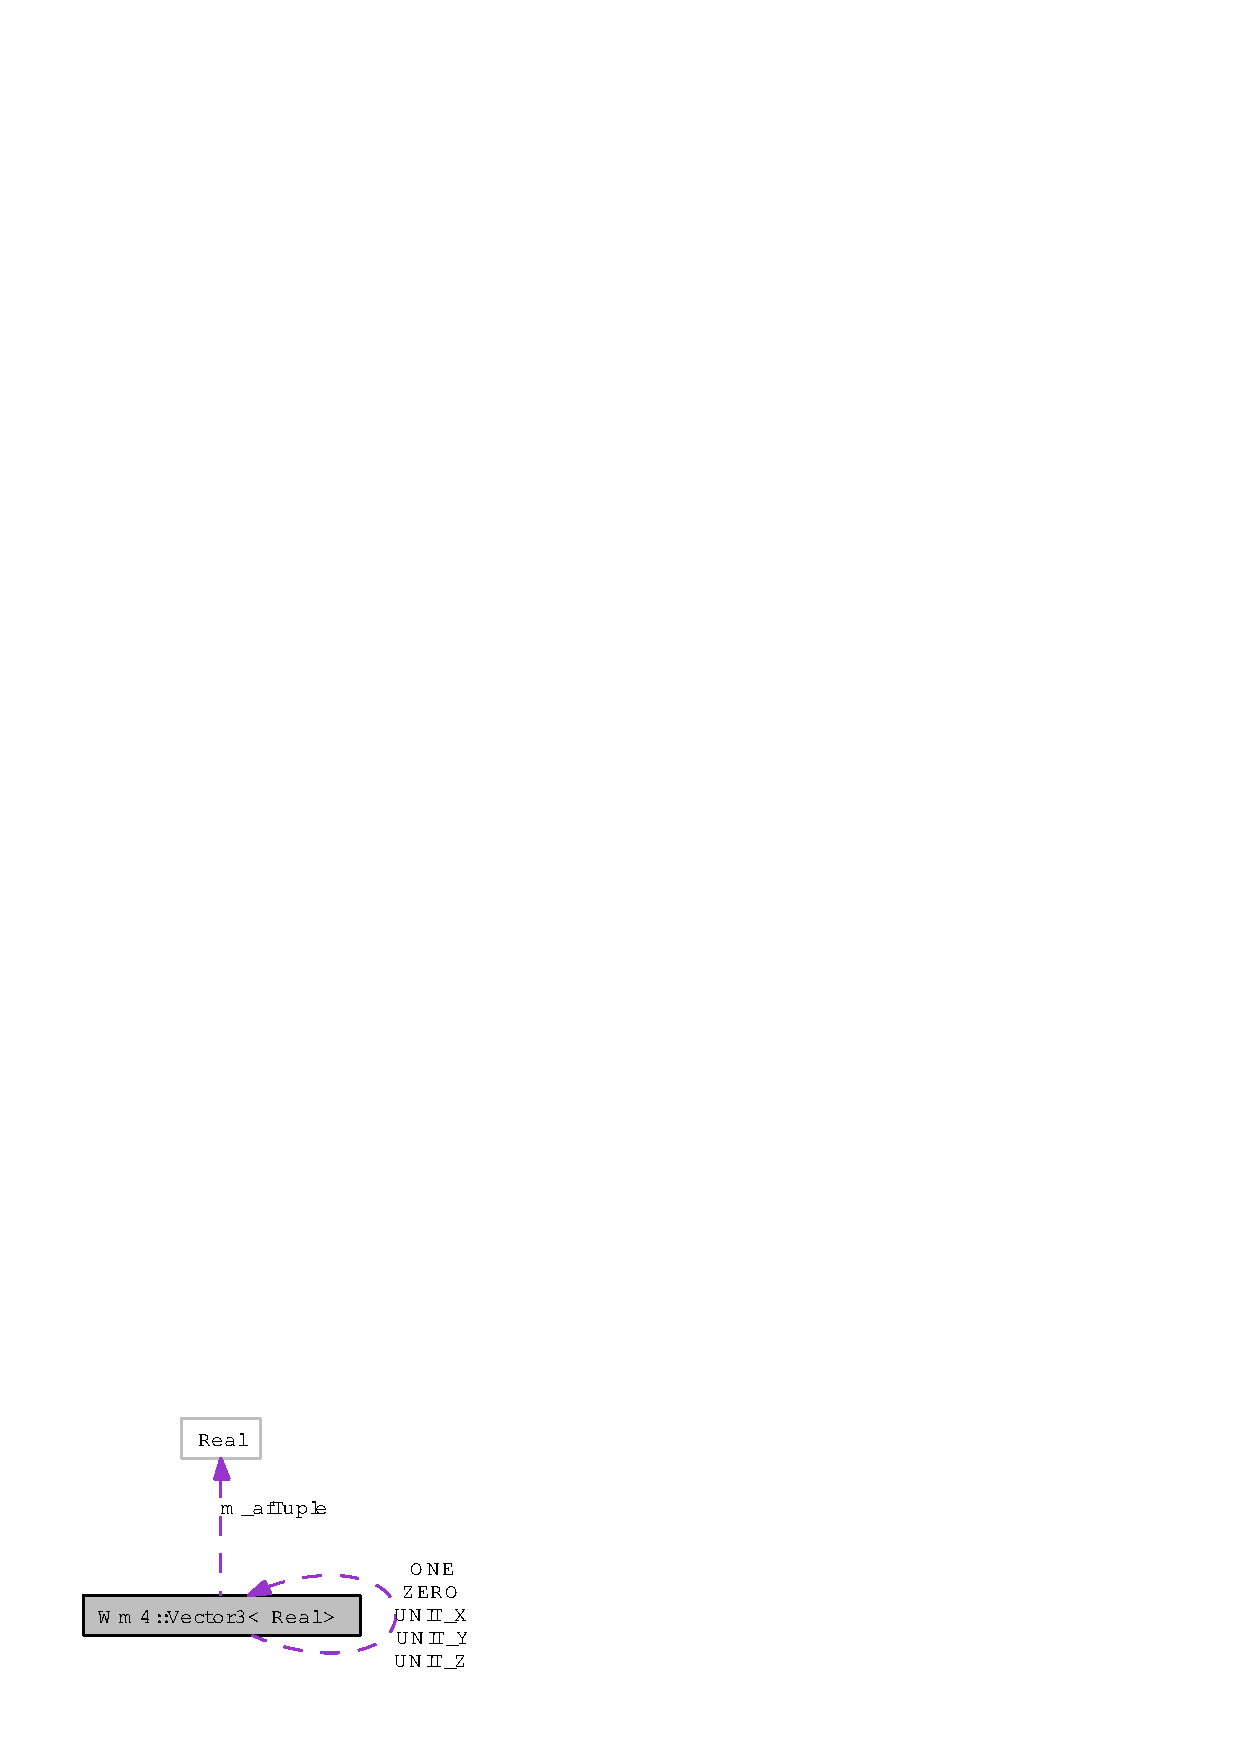
\includegraphics[width=115pt]{classWm4_1_1Vector3__coll__graph}
\end{center}
\end{figure}
\subsection*{Public Member Functions}
\begin{CompactItemize}
\item 
{\bf Vector3} ()
\item 
{\bf Vector3} (Real f\-X, Real f\-Y, Real f\-Z)
\item 
{\bf Vector3} (const Real $\ast$af\-Tuple)
\item 
{\bf Vector3} (const {\bf Vector3} \&rk\-V)
\item 
{\bf operator const Real $\ast$} () const
\item 
{\bf operator Real $\ast$} ()
\item 
Real {\bf operator[$\,$]} (int i) const
\item 
Real \& {\bf operator[$\,$]} (int i)
\item 
Real {\bf X} () const
\item 
Real \& {\bf X} ()
\item 
Real {\bf Y} () const
\item 
Real \& {\bf Y} ()
\item 
Real {\bf Z} () const
\item 
Real \& {\bf Z} ()
\item 
{\bf Vector3} \& {\bf operator=} (const {\bf Vector3} \&rk\-V)
\item 
bool {\bf operator==} (const {\bf Vector3} \&rk\-V) const
\item 
bool {\bf operator!=} (const {\bf Vector3} \&rk\-V) const
\item 
bool {\bf operator$<$} (const {\bf Vector3} \&rk\-V) const
\item 
bool {\bf operator$<$=} (const {\bf Vector3} \&rk\-V) const
\item 
bool {\bf operator$>$} (const {\bf Vector3} \&rk\-V) const
\item 
bool {\bf operator$>$=} (const {\bf Vector3} \&rk\-V) const
\item 
{\bf Vector3} {\bf operator+} (const {\bf Vector3} \&rk\-V) const
\item 
{\bf Vector3} {\bf operator-} (const {\bf Vector3} \&rk\-V) const
\item 
{\bf Vector3} {\bf operator $\ast$} (Real f\-Scalar) const 
\item 
{\bf Vector3} {\bf operator/} (Real f\-Scalar) const 
\item 
{\bf Vector3} {\bf operator-} () const
\item 
{\bf Vector3} \& {\bf operator+=} (const {\bf Vector3} \&rk\-V)
\item 
{\bf Vector3} \& {\bf operator-=} (const {\bf Vector3} \&rk\-V)
\item 
{\bf Vector3} \& {\bf operator $\ast$=} (Real f\-Scalar)
\item 
{\bf Vector3} \& {\bf operator/=} (Real f\-Scalar)
\item 
Real {\bf Length} () const
\item 
Real {\bf Squared\-Length} () const
\item 
Real {\bf Dot} (const {\bf Vector3} \&rk\-V) const
\item 
Real {\bf Normalize} ()
\item 
{\bf Vector3} {\bf Cross} (const {\bf Vector3} \&rk\-V) const
\item 
{\bf Vector3} {\bf Unit\-Cross} (const {\bf Vector3} \&rk\-V) const
\item 
void {\bf Get\-Barycentrics} (const {\bf Vector3} \&rk\-V0, const {\bf Vector3} \&rk\-V1, const {\bf Vector3} \&rk\-V2, const {\bf Vector3} \&rk\-V3, Real af\-Bary[4]) const
\end{CompactItemize}
\subsection*{Static Public Member Functions}
\begin{CompactItemize}
\item 
static void {\bf Orthonormalize} ({\bf Vector3} \&rk\-U, {\bf Vector3} \&rk\-V, {\bf Vector3} \&rk\-W)
\item 
static void {\bf Orthonormalize} ({\bf Vector3} $\ast$ak\-V)
\item 
static void {\bf Generate\-Orthonormal\-Basis} ({\bf Vector3} \&rk\-U, {\bf Vector3} \&rk\-V, {\bf Vector3} \&rk\-W)
\item 
static void {\bf Generate\-Complement\-Basis} ({\bf Vector3} \&rk\-U, {\bf Vector3} \&rk\-V, const {\bf Vector3} \&rk\-W)
\item 
static void {\bf Compute\-Extremes} (int i\-VQuantity, const {\bf Vector3} $\ast$ak\-Point, {\bf Vector3} \&rk\-Min, {\bf Vector3} \&rk\-Max)
\end{CompactItemize}
\subsection*{Static Public Attributes}
\begin{CompactItemize}
\item 
static WM4\_\-FOUNDATION\_\-ITEM const {\bf Vector3} {\bf ZERO}
\item 
static WM4\_\-FOUNDATION\_\-ITEM const {\bf Vector3} {\bf UNIT\_\-X}
\item 
static WM4\_\-FOUNDATION\_\-ITEM const {\bf Vector3} {\bf UNIT\_\-Y}
\item 
static WM4\_\-FOUNDATION\_\-ITEM const {\bf Vector3} {\bf UNIT\_\-Z}
\item 
static WM4\_\-FOUNDATION\_\-ITEM const {\bf Vector3} {\bf ONE}
\end{CompactItemize}
\subsubsection*{template$<$class Real$>$ class Wm4::Vector3$<$ Real $>$}



\subsection{Constructor \& Destructor Documentation}
\index{Wm4::Vector3@{Wm4::Vector3}!Vector3@{Vector3}}
\index{Vector3@{Vector3}!Wm4::Vector3@{Wm4::Vector3}}
\subsubsection{\setlength{\rightskip}{0pt plus 5cm}template$<$class Real$>$ {\bf Wm4::Vector3}$<$ Real $>$::{\bf Vector3} ()}\label{classWm4_1_1Vector3_0be5457c1a2ed752bd762a343fff6966}


\index{Wm4::Vector3@{Wm4::Vector3}!Vector3@{Vector3}}
\index{Vector3@{Vector3}!Wm4::Vector3@{Wm4::Vector3}}
\subsubsection{\setlength{\rightskip}{0pt plus 5cm}template$<$class Real$>$ {\bf Wm4::Vector3}$<$ Real $>$::{\bf Vector3} (Real {\em f\-X}, Real {\em f\-Y}, Real {\em f\-Z})}\label{classWm4_1_1Vector3_c447f97781c24e59be04539611a59e56}


\index{Wm4::Vector3@{Wm4::Vector3}!Vector3@{Vector3}}
\index{Vector3@{Vector3}!Wm4::Vector3@{Wm4::Vector3}}
\subsubsection{\setlength{\rightskip}{0pt plus 5cm}template$<$class Real$>$ {\bf Wm4::Vector3}$<$ Real $>$::{\bf Vector3} (const Real $\ast$ {\em af\-Tuple})}\label{classWm4_1_1Vector3_1c8c298fef9dacf92a789178878d4803}


\index{Wm4::Vector3@{Wm4::Vector3}!Vector3@{Vector3}}
\index{Vector3@{Vector3}!Wm4::Vector3@{Wm4::Vector3}}
\subsubsection{\setlength{\rightskip}{0pt plus 5cm}template$<$class Real$>$ {\bf Wm4::Vector3}$<$ Real $>$::{\bf Vector3} (const {\bf Vector3}$<$ Real $>$ \& {\em rk\-V})}\label{classWm4_1_1Vector3_e231716c3dd5d198ad17ef0c55cdd90b}




\subsection{Member Function Documentation}
\index{Wm4::Vector3@{Wm4::Vector3}!operator const Real *@{operator const Real $\ast$}}
\index{operator const Real *@{operator const Real $\ast$}!Wm4::Vector3@{Wm4::Vector3}}
\subsubsection{\setlength{\rightskip}{0pt plus 5cm}template$<$class Real$>$ {\bf Wm4::Vector3}$<$ Real $>$::operator const Real $\ast$ () const\hspace{0.3cm}{\tt  [inline]}}\label{classWm4_1_1Vector3_55e31edc3b1cf7fd110ec88b09863829}


\index{Wm4::Vector3@{Wm4::Vector3}!operator Real *@{operator Real $\ast$}}
\index{operator Real *@{operator Real $\ast$}!Wm4::Vector3@{Wm4::Vector3}}
\subsubsection{\setlength{\rightskip}{0pt plus 5cm}template$<$class Real$>$ {\bf Wm4::Vector3}$<$ Real $>$::operator Real $\ast$ ()\hspace{0.3cm}{\tt  [inline]}}\label{classWm4_1_1Vector3_496ff7239bd1c34d7094ad0d963baf94}


\index{Wm4::Vector3@{Wm4::Vector3}!operator[]@{operator[]}}
\index{operator[]@{operator[]}!Wm4::Vector3@{Wm4::Vector3}}
\subsubsection{\setlength{\rightskip}{0pt plus 5cm}template$<$class Real$>$ Real {\bf Wm4::Vector3}$<$ Real $>$::operator[$\,$] (int {\em i}) const\hspace{0.3cm}{\tt  [inline]}}\label{classWm4_1_1Vector3_3a1e926dc747b7ba08728e2b89348618}


\index{Wm4::Vector3@{Wm4::Vector3}!operator[]@{operator[]}}
\index{operator[]@{operator[]}!Wm4::Vector3@{Wm4::Vector3}}
\subsubsection{\setlength{\rightskip}{0pt plus 5cm}template$<$class Real$>$ Real \& {\bf Wm4::Vector3}$<$ Real $>$::operator[$\,$] (int {\em i})\hspace{0.3cm}{\tt  [inline]}}\label{classWm4_1_1Vector3_f16c1aab5c89b902d4c374fd8ab18f73}


\index{Wm4::Vector3@{Wm4::Vector3}!X@{X}}
\index{X@{X}!Wm4::Vector3@{Wm4::Vector3}}
\subsubsection{\setlength{\rightskip}{0pt plus 5cm}template$<$class Real$>$ Real {\bf Wm4::Vector3}$<$ Real $>$::X () const\hspace{0.3cm}{\tt  [inline]}}\label{classWm4_1_1Vector3_3854b82c9d1ebea73073c5a523abde3b}


\index{Wm4::Vector3@{Wm4::Vector3}!X@{X}}
\index{X@{X}!Wm4::Vector3@{Wm4::Vector3}}
\subsubsection{\setlength{\rightskip}{0pt plus 5cm}template$<$class Real$>$ Real \& {\bf Wm4::Vector3}$<$ Real $>$::X ()\hspace{0.3cm}{\tt  [inline]}}\label{classWm4_1_1Vector3_a63221cc2c958bdda340a7f7f08da6a8}


\index{Wm4::Vector3@{Wm4::Vector3}!Y@{Y}}
\index{Y@{Y}!Wm4::Vector3@{Wm4::Vector3}}
\subsubsection{\setlength{\rightskip}{0pt plus 5cm}template$<$class Real$>$ Real {\bf Wm4::Vector3}$<$ Real $>$::Y () const\hspace{0.3cm}{\tt  [inline]}}\label{classWm4_1_1Vector3_4d9580d763d3710cb58316d769daa6a9}


\index{Wm4::Vector3@{Wm4::Vector3}!Y@{Y}}
\index{Y@{Y}!Wm4::Vector3@{Wm4::Vector3}}
\subsubsection{\setlength{\rightskip}{0pt plus 5cm}template$<$class Real$>$ Real \& {\bf Wm4::Vector3}$<$ Real $>$::Y ()\hspace{0.3cm}{\tt  [inline]}}\label{classWm4_1_1Vector3_ed0ce037680d2e5c19df316d620b19f8}


\index{Wm4::Vector3@{Wm4::Vector3}!Z@{Z}}
\index{Z@{Z}!Wm4::Vector3@{Wm4::Vector3}}
\subsubsection{\setlength{\rightskip}{0pt plus 5cm}template$<$class Real$>$ Real {\bf Wm4::Vector3}$<$ Real $>$::Z () const\hspace{0.3cm}{\tt  [inline]}}\label{classWm4_1_1Vector3_69fce1c602b0b8568d41d05a3ef4088b}


\index{Wm4::Vector3@{Wm4::Vector3}!Z@{Z}}
\index{Z@{Z}!Wm4::Vector3@{Wm4::Vector3}}
\subsubsection{\setlength{\rightskip}{0pt plus 5cm}template$<$class Real$>$ Real \& {\bf Wm4::Vector3}$<$ Real $>$::Z ()\hspace{0.3cm}{\tt  [inline]}}\label{classWm4_1_1Vector3_792db4bd00e018eea9d3be13506b6558}


\index{Wm4::Vector3@{Wm4::Vector3}!operator=@{operator=}}
\index{operator=@{operator=}!Wm4::Vector3@{Wm4::Vector3}}
\subsubsection{\setlength{\rightskip}{0pt plus 5cm}template$<$class Real$>$ {\bf Vector3}$<$ Real $>$ \& {\bf Wm4::Vector3}$<$ Real $>$::operator= (const {\bf Vector3}$<$ Real $>$ \& {\em rk\-V})\hspace{0.3cm}{\tt  [inline]}}\label{classWm4_1_1Vector3_4c462b662e2453a855d2216ae00d4eb1}


\index{Wm4::Vector3@{Wm4::Vector3}!operator==@{operator==}}
\index{operator==@{operator==}!Wm4::Vector3@{Wm4::Vector3}}
\subsubsection{\setlength{\rightskip}{0pt plus 5cm}template$<$class Real$>$ bool {\bf Wm4::Vector3}$<$ Real $>$::operator== (const {\bf Vector3}$<$ Real $>$ \& {\em rk\-V}) const}\label{classWm4_1_1Vector3_f627f662808c5603863d2d7c4202c60a}


\index{Wm4::Vector3@{Wm4::Vector3}!operator"!=@{operator"!=}}
\index{operator"!=@{operator"!=}!Wm4::Vector3@{Wm4::Vector3}}
\subsubsection{\setlength{\rightskip}{0pt plus 5cm}template$<$class Real$>$ bool {\bf Wm4::Vector3}$<$ Real $>$::operator!= (const {\bf Vector3}$<$ Real $>$ \& {\em rk\-V}) const}\label{classWm4_1_1Vector3_397a06523c9a33ca92ccf5c3edd172d5}


\index{Wm4::Vector3@{Wm4::Vector3}!operator<@{operator$<$}}
\index{operator<@{operator$<$}!Wm4::Vector3@{Wm4::Vector3}}
\subsubsection{\setlength{\rightskip}{0pt plus 5cm}template$<$class Real$>$ bool {\bf Wm4::Vector3}$<$ Real $>$::operator$<$ (const {\bf Vector3}$<$ Real $>$ \& {\em rk\-V}) const}\label{classWm4_1_1Vector3_3e9a9c63a62a44e5745aeb9071bf4f55}


\index{Wm4::Vector3@{Wm4::Vector3}!operator<=@{operator$<$=}}
\index{operator<=@{operator$<$=}!Wm4::Vector3@{Wm4::Vector3}}
\subsubsection{\setlength{\rightskip}{0pt plus 5cm}template$<$class Real$>$ bool {\bf Wm4::Vector3}$<$ Real $>$::operator$<$= (const {\bf Vector3}$<$ Real $>$ \& {\em rk\-V}) const}\label{classWm4_1_1Vector3_7800f2c726bd9eb09892f767cd7aba19}


\index{Wm4::Vector3@{Wm4::Vector3}!operator>@{operator$>$}}
\index{operator>@{operator$>$}!Wm4::Vector3@{Wm4::Vector3}}
\subsubsection{\setlength{\rightskip}{0pt plus 5cm}template$<$class Real$>$ bool {\bf Wm4::Vector3}$<$ Real $>$::operator$>$ (const {\bf Vector3}$<$ Real $>$ \& {\em rk\-V}) const}\label{classWm4_1_1Vector3_023cea9ce14058000639c93290ca4295}


\index{Wm4::Vector3@{Wm4::Vector3}!operator>=@{operator$>$=}}
\index{operator>=@{operator$>$=}!Wm4::Vector3@{Wm4::Vector3}}
\subsubsection{\setlength{\rightskip}{0pt plus 5cm}template$<$class Real$>$ bool {\bf Wm4::Vector3}$<$ Real $>$::operator$>$= (const {\bf Vector3}$<$ Real $>$ \& {\em rk\-V}) const}\label{classWm4_1_1Vector3_4854e5f3f495c178e471cda42d896224}


\index{Wm4::Vector3@{Wm4::Vector3}!operator+@{operator+}}
\index{operator+@{operator+}!Wm4::Vector3@{Wm4::Vector3}}
\subsubsection{\setlength{\rightskip}{0pt plus 5cm}template$<$class Real$>$ {\bf Vector3}$<$ Real $>$ {\bf Wm4::Vector3}$<$ Real $>$::operator+ (const {\bf Vector3}$<$ Real $>$ \& {\em rk\-V}) const\hspace{0.3cm}{\tt  [inline]}}\label{classWm4_1_1Vector3_e771fc04c155a10e188bcf2e2b957676}


\index{Wm4::Vector3@{Wm4::Vector3}!operator-@{operator-}}
\index{operator-@{operator-}!Wm4::Vector3@{Wm4::Vector3}}
\subsubsection{\setlength{\rightskip}{0pt plus 5cm}template$<$class Real$>$ {\bf Vector3}$<$ Real $>$ {\bf Wm4::Vector3}$<$ Real $>$::operator- (const {\bf Vector3}$<$ Real $>$ \& {\em rk\-V}) const\hspace{0.3cm}{\tt  [inline]}}\label{classWm4_1_1Vector3_fd35acae902bdf5171c4ae77ecee371e}


\index{Wm4::Vector3@{Wm4::Vector3}!operator *@{operator $\ast$}}
\index{operator *@{operator $\ast$}!Wm4::Vector3@{Wm4::Vector3}}
\subsubsection{\setlength{\rightskip}{0pt plus 5cm}template$<$class Real$>$ {\bf Vector3}$<$ Real $>$ {\bf Wm4::Vector3}$<$ Real $>$::operator $\ast$ (Real {\em f\-Scalar}) const\hspace{0.3cm}{\tt  [inline]}}\label{classWm4_1_1Vector3_8daebcb3f93401a705b1fa0e00591fd2}


\index{Wm4::Vector3@{Wm4::Vector3}!operator/@{operator/}}
\index{operator/@{operator/}!Wm4::Vector3@{Wm4::Vector3}}
\subsubsection{\setlength{\rightskip}{0pt plus 5cm}template$<$class Real$>$ {\bf Vector3}$<$ Real $>$ {\bf Wm4::Vector3}$<$ Real $>$::operator/ (Real {\em f\-Scalar}) const\hspace{0.3cm}{\tt  [inline]}}\label{classWm4_1_1Vector3_6ad5c9c95d41fca84ef29b56367a4dd7}


\index{Wm4::Vector3@{Wm4::Vector3}!operator-@{operator-}}
\index{operator-@{operator-}!Wm4::Vector3@{Wm4::Vector3}}
\subsubsection{\setlength{\rightskip}{0pt plus 5cm}template$<$class Real$>$ {\bf Vector3}$<$ Real $>$ {\bf Wm4::Vector3}$<$ Real $>$::operator- () const\hspace{0.3cm}{\tt  [inline]}}\label{classWm4_1_1Vector3_7e96a2252e4e8feec613ff6c11630f23}


\index{Wm4::Vector3@{Wm4::Vector3}!operator+=@{operator+=}}
\index{operator+=@{operator+=}!Wm4::Vector3@{Wm4::Vector3}}
\subsubsection{\setlength{\rightskip}{0pt plus 5cm}template$<$class Real$>$ {\bf Vector3}$<$ Real $>$ \& {\bf Wm4::Vector3}$<$ Real $>$::operator+= (const {\bf Vector3}$<$ Real $>$ \& {\em rk\-V})\hspace{0.3cm}{\tt  [inline]}}\label{classWm4_1_1Vector3_2b60ed421e03409beca697cfefe775a0}


\index{Wm4::Vector3@{Wm4::Vector3}!operator-=@{operator-=}}
\index{operator-=@{operator-=}!Wm4::Vector3@{Wm4::Vector3}}
\subsubsection{\setlength{\rightskip}{0pt plus 5cm}template$<$class Real$>$ {\bf Vector3}$<$ Real $>$ \& {\bf Wm4::Vector3}$<$ Real $>$::operator-= (const {\bf Vector3}$<$ Real $>$ \& {\em rk\-V})\hspace{0.3cm}{\tt  [inline]}}\label{classWm4_1_1Vector3_1f4f8be55361c48ce563410ca3fa1f9e}


\index{Wm4::Vector3@{Wm4::Vector3}!operator *=@{operator $\ast$=}}
\index{operator *=@{operator $\ast$=}!Wm4::Vector3@{Wm4::Vector3}}
\subsubsection{\setlength{\rightskip}{0pt plus 5cm}template$<$class Real$>$ {\bf Vector3}$<$ Real $>$ \& {\bf Wm4::Vector3}$<$ Real $>$::operator $\ast$= (Real {\em f\-Scalar})\hspace{0.3cm}{\tt  [inline]}}\label{classWm4_1_1Vector3_5bc60c9ce1bee914f39aeea3ae0294e4}


\index{Wm4::Vector3@{Wm4::Vector3}!operator/=@{operator/=}}
\index{operator/=@{operator/=}!Wm4::Vector3@{Wm4::Vector3}}
\subsubsection{\setlength{\rightskip}{0pt plus 5cm}template$<$class Real$>$ {\bf Vector3}$<$ Real $>$ \& {\bf Wm4::Vector3}$<$ Real $>$::operator/= (Real {\em f\-Scalar})\hspace{0.3cm}{\tt  [inline]}}\label{classWm4_1_1Vector3_908362502ff0c1f68d407566903c647f}


\index{Wm4::Vector3@{Wm4::Vector3}!Length@{Length}}
\index{Length@{Length}!Wm4::Vector3@{Wm4::Vector3}}
\subsubsection{\setlength{\rightskip}{0pt plus 5cm}template$<$class Real$>$ Real {\bf Wm4::Vector3}$<$ Real $>$::Length () const\hspace{0.3cm}{\tt  [inline]}}\label{classWm4_1_1Vector3_e5d946478a3e33ad6d85fafa8da99bb1}


\index{Wm4::Vector3@{Wm4::Vector3}!SquaredLength@{SquaredLength}}
\index{SquaredLength@{SquaredLength}!Wm4::Vector3@{Wm4::Vector3}}
\subsubsection{\setlength{\rightskip}{0pt plus 5cm}template$<$class Real$>$ Real {\bf Wm4::Vector3}$<$ Real $>$::Squared\-Length () const\hspace{0.3cm}{\tt  [inline]}}\label{classWm4_1_1Vector3_2b406327430121a450911b17f960c5b4}


\index{Wm4::Vector3@{Wm4::Vector3}!Dot@{Dot}}
\index{Dot@{Dot}!Wm4::Vector3@{Wm4::Vector3}}
\subsubsection{\setlength{\rightskip}{0pt plus 5cm}template$<$class Real$>$ Real {\bf Wm4::Vector3}$<$ Real $>$::Dot (const {\bf Vector3}$<$ Real $>$ \& {\em rk\-V}) const\hspace{0.3cm}{\tt  [inline]}}\label{classWm4_1_1Vector3_6dc2a1dd851f3d1f8dee786db35b9625}


\index{Wm4::Vector3@{Wm4::Vector3}!Normalize@{Normalize}}
\index{Normalize@{Normalize}!Wm4::Vector3@{Wm4::Vector3}}
\subsubsection{\setlength{\rightskip}{0pt plus 5cm}template$<$class Real$>$ Real {\bf Wm4::Vector3}$<$ Real $>$::Normalize ()\hspace{0.3cm}{\tt  [inline]}}\label{classWm4_1_1Vector3_67c6c5439a4e931d65aefd3146a61a4c}


\index{Wm4::Vector3@{Wm4::Vector3}!Cross@{Cross}}
\index{Cross@{Cross}!Wm4::Vector3@{Wm4::Vector3}}
\subsubsection{\setlength{\rightskip}{0pt plus 5cm}template$<$class Real$>$ {\bf Vector3}$<$ Real $>$ {\bf Wm4::Vector3}$<$ Real $>$::Cross (const {\bf Vector3}$<$ Real $>$ \& {\em rk\-V}) const\hspace{0.3cm}{\tt  [inline]}}\label{classWm4_1_1Vector3_3aecdfd8f7e168f52232399b8e146ba0}


\index{Wm4::Vector3@{Wm4::Vector3}!UnitCross@{UnitCross}}
\index{UnitCross@{UnitCross}!Wm4::Vector3@{Wm4::Vector3}}
\subsubsection{\setlength{\rightskip}{0pt plus 5cm}template$<$class Real$>$ {\bf Vector3}$<$ Real $>$ {\bf Wm4::Vector3}$<$ Real $>$::Unit\-Cross (const {\bf Vector3}$<$ Real $>$ \& {\em rk\-V}) const\hspace{0.3cm}{\tt  [inline]}}\label{classWm4_1_1Vector3_760e0d47e71eca3208faaa4790123cfe}


\index{Wm4::Vector3@{Wm4::Vector3}!GetBarycentrics@{GetBarycentrics}}
\index{GetBarycentrics@{GetBarycentrics}!Wm4::Vector3@{Wm4::Vector3}}
\subsubsection{\setlength{\rightskip}{0pt plus 5cm}template$<$class Real$>$ void {\bf Wm4::Vector3}$<$ Real $>$::Get\-Barycentrics (const {\bf Vector3}$<$ Real $>$ \& {\em rk\-V0}, const {\bf Vector3}$<$ Real $>$ \& {\em rk\-V1}, const {\bf Vector3}$<$ Real $>$ \& {\em rk\-V2}, const {\bf Vector3}$<$ Real $>$ \& {\em rk\-V3}, Real {\em af\-Bary}[4]) const}\label{classWm4_1_1Vector3_903164705e7c42dcc3040b7f53652d6d}


\index{Wm4::Vector3@{Wm4::Vector3}!Orthonormalize@{Orthonormalize}}
\index{Orthonormalize@{Orthonormalize}!Wm4::Vector3@{Wm4::Vector3}}
\subsubsection{\setlength{\rightskip}{0pt plus 5cm}template$<$class Real$>$ void {\bf Wm4::Vector3}$<$ Real $>$::Orthonormalize ({\bf Vector3}$<$ Real $>$ \& {\em rk\-U}, {\bf Vector3}$<$ Real $>$ \& {\em rk\-V}, {\bf Vector3}$<$ Real $>$ \& {\em rk\-W})\hspace{0.3cm}{\tt  [static]}}\label{classWm4_1_1Vector3_0683c0eb8409e5aae3d97e6eef388b40}


\index{Wm4::Vector3@{Wm4::Vector3}!Orthonormalize@{Orthonormalize}}
\index{Orthonormalize@{Orthonormalize}!Wm4::Vector3@{Wm4::Vector3}}
\subsubsection{\setlength{\rightskip}{0pt plus 5cm}template$<$class Real$>$ void {\bf Wm4::Vector3}$<$ Real $>$::Orthonormalize ({\bf Vector3}$<$ Real $>$ $\ast$ {\em ak\-V})\hspace{0.3cm}{\tt  [static]}}\label{classWm4_1_1Vector3_aa8d8a7ed438b61bf2bda96cf692b809}


\index{Wm4::Vector3@{Wm4::Vector3}!GenerateOrthonormalBasis@{GenerateOrthonormalBasis}}
\index{GenerateOrthonormalBasis@{GenerateOrthonormalBasis}!Wm4::Vector3@{Wm4::Vector3}}
\subsubsection{\setlength{\rightskip}{0pt plus 5cm}template$<$class Real$>$ void {\bf Wm4::Vector3}$<$ Real $>$::Generate\-Orthonormal\-Basis ({\bf Vector3}$<$ Real $>$ \& {\em rk\-U}, {\bf Vector3}$<$ Real $>$ \& {\em rk\-V}, {\bf Vector3}$<$ Real $>$ \& {\em rk\-W})\hspace{0.3cm}{\tt  [static]}}\label{classWm4_1_1Vector3_c02acfd8ea2501022b8408085db2f78a}


\index{Wm4::Vector3@{Wm4::Vector3}!GenerateComplementBasis@{GenerateComplementBasis}}
\index{GenerateComplementBasis@{GenerateComplementBasis}!Wm4::Vector3@{Wm4::Vector3}}
\subsubsection{\setlength{\rightskip}{0pt plus 5cm}template$<$class Real$>$ void {\bf Wm4::Vector3}$<$ Real $>$::Generate\-Complement\-Basis ({\bf Vector3}$<$ Real $>$ \& {\em rk\-U}, {\bf Vector3}$<$ Real $>$ \& {\em rk\-V}, const {\bf Vector3}$<$ Real $>$ \& {\em rk\-W})\hspace{0.3cm}{\tt  [static]}}\label{classWm4_1_1Vector3_c9d9839d0871bfe560834eec756125b5}


\index{Wm4::Vector3@{Wm4::Vector3}!ComputeExtremes@{ComputeExtremes}}
\index{ComputeExtremes@{ComputeExtremes}!Wm4::Vector3@{Wm4::Vector3}}
\subsubsection{\setlength{\rightskip}{0pt plus 5cm}template$<$class Real$>$ void {\bf Wm4::Vector3}$<$ Real $>$::Compute\-Extremes (int {\em i\-VQuantity}, const {\bf Vector3}$<$ Real $>$ $\ast$ {\em ak\-Point}, {\bf Vector3}$<$ Real $>$ \& {\em rk\-Min}, {\bf Vector3}$<$ Real $>$ \& {\em rk\-Max})\hspace{0.3cm}{\tt  [static]}}\label{classWm4_1_1Vector3_1233f448d7976cbf265253e79c9cfa7c}




\subsection{Member Data Documentation}
\index{Wm4::Vector3@{Wm4::Vector3}!ZERO@{ZERO}}
\index{ZERO@{ZERO}!Wm4::Vector3@{Wm4::Vector3}}
\subsubsection{\setlength{\rightskip}{0pt plus 5cm}template$<$class Real$>$ WM4\_\-FOUNDATION\_\-ITEM const {\bf Vector3} {\bf Wm4::Vector3}$<$ Real $>$::{\bf ZERO}\hspace{0.3cm}{\tt  [static]}}\label{classWm4_1_1Vector3_f350845e64d6c0bbd9d9ee1a3e71c579}


\index{Wm4::Vector3@{Wm4::Vector3}!UNIT_X@{UNIT\_\-X}}
\index{UNIT_X@{UNIT\_\-X}!Wm4::Vector3@{Wm4::Vector3}}
\subsubsection{\setlength{\rightskip}{0pt plus 5cm}template$<$class Real$>$ WM4\_\-FOUNDATION\_\-ITEM const {\bf Vector3} {\bf Wm4::Vector3}$<$ Real $>$::{\bf UNIT\_\-X}\hspace{0.3cm}{\tt  [static]}}\label{classWm4_1_1Vector3_e0d46e617795d333aad32b1281e80f5f}


\index{Wm4::Vector3@{Wm4::Vector3}!UNIT_Y@{UNIT\_\-Y}}
\index{UNIT_Y@{UNIT\_\-Y}!Wm4::Vector3@{Wm4::Vector3}}
\subsubsection{\setlength{\rightskip}{0pt plus 5cm}template$<$class Real$>$ WM4\_\-FOUNDATION\_\-ITEM const {\bf Vector3} {\bf Wm4::Vector3}$<$ Real $>$::{\bf UNIT\_\-Y}\hspace{0.3cm}{\tt  [static]}}\label{classWm4_1_1Vector3_4ae2bc6a0a63b061c4776ca47af8f8c3}


\index{Wm4::Vector3@{Wm4::Vector3}!UNIT_Z@{UNIT\_\-Z}}
\index{UNIT_Z@{UNIT\_\-Z}!Wm4::Vector3@{Wm4::Vector3}}
\subsubsection{\setlength{\rightskip}{0pt plus 5cm}template$<$class Real$>$ WM4\_\-FOUNDATION\_\-ITEM const {\bf Vector3} {\bf Wm4::Vector3}$<$ Real $>$::{\bf UNIT\_\-Z}\hspace{0.3cm}{\tt  [static]}}\label{classWm4_1_1Vector3_8fbb0d29c3baae4c939e9383bf3d7873}


\index{Wm4::Vector3@{Wm4::Vector3}!ONE@{ONE}}
\index{ONE@{ONE}!Wm4::Vector3@{Wm4::Vector3}}
\subsubsection{\setlength{\rightskip}{0pt plus 5cm}template$<$class Real$>$ WM4\_\-FOUNDATION\_\-ITEM const {\bf Vector3} {\bf Wm4::Vector3}$<$ Real $>$::{\bf ONE}\hspace{0.3cm}{\tt  [static]}}\label{classWm4_1_1Vector3_405bef51c93e62b6fc50f54ba12ffa72}




The documentation for this class was generated from the following file:\begin{CompactItemize}
\item 
{\bf Wm4Vector3.h}\end{CompactItemize}

\section{hxa7241\_\-graphics::Vector3r Class Reference}
\label{classhxa7241__graphics_1_1Vector3r}\index{hxa7241_graphics::Vector3r@{hxa7241\_\-graphics::Vector3r}}
{\tt \#include $<$Vector3r.h$>$}

\subsection*{Public Member Functions}
\begin{CompactItemize}
\item 
{\bf Vector3r} ()
\begin{CompactList}\small\item\em standard object services --------------------------------------------------- \item\end{CompactList}\item 
{\bf Vector3r} (real x, real y, real z)
\item 
{\bf $\sim$Vector3r} ()
\begin{CompactList}\small\item\em standard object services --------------------------------------------------- \item\end{CompactList}\item 
{\bf Vector3r} (const {\bf Vector3r} \&)
\item 
{\bf Vector3r} \& {\bf operator=} (const {\bf Vector3r} \&)
\item 
{\bf Vector3r} \& {\bf set} (real x, real y, real z)
\begin{CompactList}\small\item\em commands ------------------------------------------------------------------- \item\end{CompactList}\item 
{\bf Vector3r} \& {\bf operator+=} (const {\bf Vector3r} \&)
\item 
{\bf Vector3r} \& {\bf operator-=} (const {\bf Vector3r} \&)
\item 
{\bf Vector3r} \& {\bf operator $\ast$=} (const {\bf Vector3r} \&)
\item 
{\bf Vector3r} \& {\bf operator/=} (const {\bf Vector3r} \&)
\item 
{\bf Vector3r} \& {\bf operator $\ast$=} (real)
\item 
{\bf Vector3r} \& {\bf operator/=} (real)
\item 
real {\bf get\-X} () const
\begin{CompactList}\small\item\em queries -------------------------------------------------------------------- \item\end{CompactList}\item 
real {\bf get\-Y} () const
\item 
real {\bf get\-Z} () const
\item 
real {\bf operator[$\,$]} (int) const
\item 
real {\bf length} () const
\begin{CompactList}\small\item\em queries -------------------------------------------------------------------- \item\end{CompactList}\item 
{\bf Vector3r} {\bf operator+} (const {\bf Vector3r} \&) const
\item 
{\bf Vector3r} {\bf operator-} (const {\bf Vector3r} \&) const
\item 
{\bf Vector3r} {\bf operator $\ast$} (const {\bf Vector3r} \&) const
\item 
{\bf Vector3r} {\bf operator/} (const {\bf Vector3r} \&) const
\item 
{\bf Vector3r} {\bf operator $\ast$} (real) const
\item 
{\bf Vector3r} {\bf operator/} (real) const
\item 
bool {\bf operator==} (const {\bf Vector3r} \&) const
\item 
bool {\bf operator!=} (const {\bf Vector3r} \&) const
\item 
bool {\bf is\-Zero} () const
\end{CompactItemize}
\subsection*{Static Public Member Functions}
\begin{CompactItemize}
\item 
static const {\bf Vector3r} \& {\bf ZERO} ()
\begin{CompactList}\small\item\em constants ------------------------------------------------------------------ \item\end{CompactList}\item 
static const {\bf Vector3r} \& {\bf HALF} ()
\item 
static const {\bf Vector3r} \& {\bf ONE} ()
\end{CompactItemize}
\subsection*{Friends}
\begin{CompactItemize}
\item 
{\bf Vector3r} {\bf operator $\ast$} (real, const {\bf Vector3r} \&)
\begin{CompactList}\small\item\em friends -------------------------------------------------------------------- \item\end{CompactList}\item 
{\bf Vector3r} {\bf operator/} (real, const {\bf Vector3r} \&)
\end{CompactItemize}


\subsection{Detailed Description}
Yes, its the 3D vector class!.\par
\par


If you write some 3D graphics software, then you MUST write your OWN vector class -- it is the law. So here is mine.\par
\par


(Unused stuff commented-out) 



\subsection{Constructor \& Destructor Documentation}
\index{hxa7241_graphics::Vector3r@{hxa7241\_\-graphics::Vector3r}!Vector3r@{Vector3r}}
\index{Vector3r@{Vector3r}!hxa7241_graphics::Vector3r@{hxa7241\_\-graphics::Vector3r}}
\subsubsection{\setlength{\rightskip}{0pt plus 5cm}Vector3r::Vector3r ()}\label{classhxa7241__graphics_1_1Vector3r_6cafbec0341bf75076ed59bf0d63acbb}


standard object services --------------------------------------------------- 

\index{hxa7241_graphics::Vector3r@{hxa7241\_\-graphics::Vector3r}!Vector3r@{Vector3r}}
\index{Vector3r@{Vector3r}!hxa7241_graphics::Vector3r@{hxa7241\_\-graphics::Vector3r}}
\subsubsection{\setlength{\rightskip}{0pt plus 5cm}Vector3r::Vector3r (real {\em x}, real {\em y}, real {\em z})}\label{classhxa7241__graphics_1_1Vector3r_9cfb05cb51e81c00ff049ee6834f0403}


\index{hxa7241_graphics::Vector3r@{hxa7241\_\-graphics::Vector3r}!~Vector3r@{$\sim$Vector3r}}
\index{~Vector3r@{$\sim$Vector3r}!hxa7241_graphics::Vector3r@{hxa7241\_\-graphics::Vector3r}}
\subsubsection{\setlength{\rightskip}{0pt plus 5cm}hxa7241\_\-graphics::Vector3r::$\sim$Vector3r ()\hspace{0.3cm}{\tt  [inline]}}\label{classhxa7241__graphics_1_1Vector3r_da27e60869e153abecd6be5d8b5976e5}


standard object services --------------------------------------------------- 

\index{hxa7241_graphics::Vector3r@{hxa7241\_\-graphics::Vector3r}!Vector3r@{Vector3r}}
\index{Vector3r@{Vector3r}!hxa7241_graphics::Vector3r@{hxa7241\_\-graphics::Vector3r}}
\subsubsection{\setlength{\rightskip}{0pt plus 5cm}hxa7241\_\-graphics::Vector3r::Vector3r (const {\bf Vector3r} \&)\hspace{0.3cm}{\tt  [inline]}}\label{classhxa7241__graphics_1_1Vector3r_8fc672fc98a6a810dc9fd336f107f1c5}




\subsection{Member Function Documentation}
\index{hxa7241_graphics::Vector3r@{hxa7241\_\-graphics::Vector3r}!operator=@{operator=}}
\index{operator=@{operator=}!hxa7241_graphics::Vector3r@{hxa7241\_\-graphics::Vector3r}}
\subsubsection{\setlength{\rightskip}{0pt plus 5cm}{\bf Vector3r} \& Vector3r::operator= (const {\bf Vector3r} \&)}\label{classhxa7241__graphics_1_1Vector3r_20579049bbbfd50d954a22ddd4391945}


\index{hxa7241_graphics::Vector3r@{hxa7241\_\-graphics::Vector3r}!set@{set}}
\index{set@{set}!hxa7241_graphics::Vector3r@{hxa7241\_\-graphics::Vector3r}}
\subsubsection{\setlength{\rightskip}{0pt plus 5cm}{\bf Vector3r} \& Vector3r::set (real {\em x}, real {\em y}, real {\em z})}\label{classhxa7241__graphics_1_1Vector3r_5d3ee37c8dd1c169bdffcbb164bdefac}


commands ------------------------------------------------------------------- 

\index{hxa7241_graphics::Vector3r@{hxa7241\_\-graphics::Vector3r}!operator+=@{operator+=}}
\index{operator+=@{operator+=}!hxa7241_graphics::Vector3r@{hxa7241\_\-graphics::Vector3r}}
\subsubsection{\setlength{\rightskip}{0pt plus 5cm}{\bf Vector3r} \& Vector3r::operator+= (const {\bf Vector3r} \&)}\label{classhxa7241__graphics_1_1Vector3r_3d77bab12071c383eceb8a2b16ef91a7}


\index{hxa7241_graphics::Vector3r@{hxa7241\_\-graphics::Vector3r}!operator-=@{operator-=}}
\index{operator-=@{operator-=}!hxa7241_graphics::Vector3r@{hxa7241\_\-graphics::Vector3r}}
\subsubsection{\setlength{\rightskip}{0pt plus 5cm}{\bf Vector3r} \& Vector3r::operator-= (const {\bf Vector3r} \&)}\label{classhxa7241__graphics_1_1Vector3r_09a0df54d3669ca5c17902dcbe5094d0}


\index{hxa7241_graphics::Vector3r@{hxa7241\_\-graphics::Vector3r}!operator *=@{operator $\ast$=}}
\index{operator *=@{operator $\ast$=}!hxa7241_graphics::Vector3r@{hxa7241\_\-graphics::Vector3r}}
\subsubsection{\setlength{\rightskip}{0pt plus 5cm}{\bf Vector3r} \& Vector3r::operator $\ast$= (const {\bf Vector3r} \&)}\label{classhxa7241__graphics_1_1Vector3r_f18978bb00e316fd23c88e1402c63984}


\index{hxa7241_graphics::Vector3r@{hxa7241\_\-graphics::Vector3r}!operator/=@{operator/=}}
\index{operator/=@{operator/=}!hxa7241_graphics::Vector3r@{hxa7241\_\-graphics::Vector3r}}
\subsubsection{\setlength{\rightskip}{0pt plus 5cm}{\bf Vector3r} \& Vector3r::operator/= (const {\bf Vector3r} \&)}\label{classhxa7241__graphics_1_1Vector3r_d124fd080646ba1860a37eea1bc3eea0}


\index{hxa7241_graphics::Vector3r@{hxa7241\_\-graphics::Vector3r}!operator *=@{operator $\ast$=}}
\index{operator *=@{operator $\ast$=}!hxa7241_graphics::Vector3r@{hxa7241\_\-graphics::Vector3r}}
\subsubsection{\setlength{\rightskip}{0pt plus 5cm}{\bf Vector3r} \& Vector3r::operator $\ast$= (real)}\label{classhxa7241__graphics_1_1Vector3r_4cf14e4e2953f2e5e68b1a924824f923}


\index{hxa7241_graphics::Vector3r@{hxa7241\_\-graphics::Vector3r}!operator/=@{operator/=}}
\index{operator/=@{operator/=}!hxa7241_graphics::Vector3r@{hxa7241\_\-graphics::Vector3r}}
\subsubsection{\setlength{\rightskip}{0pt plus 5cm}{\bf Vector3r} \& Vector3r::operator/= (real)}\label{classhxa7241__graphics_1_1Vector3r_719ad9cd94a87a65aa3d83282ee88e0c}


\index{hxa7241_graphics::Vector3r@{hxa7241\_\-graphics::Vector3r}!getX@{getX}}
\index{getX@{getX}!hxa7241_graphics::Vector3r@{hxa7241\_\-graphics::Vector3r}}
\subsubsection{\setlength{\rightskip}{0pt plus 5cm}real hxa7241\_\-graphics::Vector3r::get\-X () const\hspace{0.3cm}{\tt  [inline]}}\label{classhxa7241__graphics_1_1Vector3r_4ce46da3e114ff6d9572df3cc432fb50}


queries -------------------------------------------------------------------- 

\index{hxa7241_graphics::Vector3r@{hxa7241\_\-graphics::Vector3r}!getY@{getY}}
\index{getY@{getY}!hxa7241_graphics::Vector3r@{hxa7241\_\-graphics::Vector3r}}
\subsubsection{\setlength{\rightskip}{0pt plus 5cm}real hxa7241\_\-graphics::Vector3r::get\-Y () const\hspace{0.3cm}{\tt  [inline]}}\label{classhxa7241__graphics_1_1Vector3r_2175ce8f7174e3b634b59f199b4746a8}


\index{hxa7241_graphics::Vector3r@{hxa7241\_\-graphics::Vector3r}!getZ@{getZ}}
\index{getZ@{getZ}!hxa7241_graphics::Vector3r@{hxa7241\_\-graphics::Vector3r}}
\subsubsection{\setlength{\rightskip}{0pt plus 5cm}real hxa7241\_\-graphics::Vector3r::get\-Z () const\hspace{0.3cm}{\tt  [inline]}}\label{classhxa7241__graphics_1_1Vector3r_5a8ca0bb9a63575efe53886967d0332b}


\index{hxa7241_graphics::Vector3r@{hxa7241\_\-graphics::Vector3r}!operator[]@{operator[]}}
\index{operator[]@{operator[]}!hxa7241_graphics::Vector3r@{hxa7241\_\-graphics::Vector3r}}
\subsubsection{\setlength{\rightskip}{0pt plus 5cm}real hxa7241\_\-graphics::Vector3r::operator[$\,$] (int) const\hspace{0.3cm}{\tt  [inline]}}\label{classhxa7241__graphics_1_1Vector3r_a1b4a2f66d02f7f4b546fd041f150a9a}


\index{hxa7241_graphics::Vector3r@{hxa7241\_\-graphics::Vector3r}!length@{length}}
\index{length@{length}!hxa7241_graphics::Vector3r@{hxa7241\_\-graphics::Vector3r}}
\subsubsection{\setlength{\rightskip}{0pt plus 5cm}real Vector3r::length () const}\label{classhxa7241__graphics_1_1Vector3r_77e3eb67cfe1401e2816aefe4b6c113c}


queries -------------------------------------------------------------------- 

\index{hxa7241_graphics::Vector3r@{hxa7241\_\-graphics::Vector3r}!operator+@{operator+}}
\index{operator+@{operator+}!hxa7241_graphics::Vector3r@{hxa7241\_\-graphics::Vector3r}}
\subsubsection{\setlength{\rightskip}{0pt plus 5cm}{\bf Vector3r} Vector3r::operator+ (const {\bf Vector3r} \&) const}\label{classhxa7241__graphics_1_1Vector3r_b8b64d276673fda88ebd60a7baa0b324}


\index{hxa7241_graphics::Vector3r@{hxa7241\_\-graphics::Vector3r}!operator-@{operator-}}
\index{operator-@{operator-}!hxa7241_graphics::Vector3r@{hxa7241\_\-graphics::Vector3r}}
\subsubsection{\setlength{\rightskip}{0pt plus 5cm}{\bf Vector3r} Vector3r::operator- (const {\bf Vector3r} \&) const}\label{classhxa7241__graphics_1_1Vector3r_e6506cc5ad885e86f5cce6576f05d2b2}


\index{hxa7241_graphics::Vector3r@{hxa7241\_\-graphics::Vector3r}!operator *@{operator $\ast$}}
\index{operator *@{operator $\ast$}!hxa7241_graphics::Vector3r@{hxa7241\_\-graphics::Vector3r}}
\subsubsection{\setlength{\rightskip}{0pt plus 5cm}{\bf Vector3r} Vector3r::operator $\ast$ (const {\bf Vector3r} \&) const}\label{classhxa7241__graphics_1_1Vector3r_928b594ea3eb7879da6c0d99f7f6fc02}


\index{hxa7241_graphics::Vector3r@{hxa7241\_\-graphics::Vector3r}!operator/@{operator/}}
\index{operator/@{operator/}!hxa7241_graphics::Vector3r@{hxa7241\_\-graphics::Vector3r}}
\subsubsection{\setlength{\rightskip}{0pt plus 5cm}{\bf Vector3r} Vector3r::operator/ (const {\bf Vector3r} \&) const}\label{classhxa7241__graphics_1_1Vector3r_c0dd36e6c73934a66b7f4003e6b5040d}


\index{hxa7241_graphics::Vector3r@{hxa7241\_\-graphics::Vector3r}!operator *@{operator $\ast$}}
\index{operator *@{operator $\ast$}!hxa7241_graphics::Vector3r@{hxa7241\_\-graphics::Vector3r}}
\subsubsection{\setlength{\rightskip}{0pt plus 5cm}{\bf Vector3r} Vector3r::operator $\ast$ (real) const}\label{classhxa7241__graphics_1_1Vector3r_d8a12132d734eacc018e8f40168f54c8}


\index{hxa7241_graphics::Vector3r@{hxa7241\_\-graphics::Vector3r}!operator/@{operator/}}
\index{operator/@{operator/}!hxa7241_graphics::Vector3r@{hxa7241\_\-graphics::Vector3r}}
\subsubsection{\setlength{\rightskip}{0pt plus 5cm}{\bf Vector3r} Vector3r::operator/ (real) const}\label{classhxa7241__graphics_1_1Vector3r_4628ccc00d308a3c887a795ab9c3e3e3}


\index{hxa7241_graphics::Vector3r@{hxa7241\_\-graphics::Vector3r}!operator==@{operator==}}
\index{operator==@{operator==}!hxa7241_graphics::Vector3r@{hxa7241\_\-graphics::Vector3r}}
\subsubsection{\setlength{\rightskip}{0pt plus 5cm}bool Vector3r::operator== (const {\bf Vector3r} \&) const}\label{classhxa7241__graphics_1_1Vector3r_7e501771d4b0c3beace144a54b79ed7b}


\index{hxa7241_graphics::Vector3r@{hxa7241\_\-graphics::Vector3r}!operator"!=@{operator"!=}}
\index{operator"!=@{operator"!=}!hxa7241_graphics::Vector3r@{hxa7241\_\-graphics::Vector3r}}
\subsubsection{\setlength{\rightskip}{0pt plus 5cm}bool Vector3r::operator!= (const {\bf Vector3r} \&) const}\label{classhxa7241__graphics_1_1Vector3r_79d4cdebbba7a719d1703adb4692317e}


\index{hxa7241_graphics::Vector3r@{hxa7241\_\-graphics::Vector3r}!isZero@{isZero}}
\index{isZero@{isZero}!hxa7241_graphics::Vector3r@{hxa7241\_\-graphics::Vector3r}}
\subsubsection{\setlength{\rightskip}{0pt plus 5cm}bool Vector3r::is\-Zero () const}\label{classhxa7241__graphics_1_1Vector3r_3d446a1cb3223d2d8918687518b55594}


\index{hxa7241_graphics::Vector3r@{hxa7241\_\-graphics::Vector3r}!ZERO@{ZERO}}
\index{ZERO@{ZERO}!hxa7241_graphics::Vector3r@{hxa7241\_\-graphics::Vector3r}}
\subsubsection{\setlength{\rightskip}{0pt plus 5cm}const {\bf Vector3r} \& Vector3r::ZERO ()\hspace{0.3cm}{\tt  [static]}}\label{classhxa7241__graphics_1_1Vector3r_6c139f56fa9d3988a0a1792b2cec98a3}


constants ------------------------------------------------------------------ 

\index{hxa7241_graphics::Vector3r@{hxa7241\_\-graphics::Vector3r}!HALF@{HALF}}
\index{HALF@{HALF}!hxa7241_graphics::Vector3r@{hxa7241\_\-graphics::Vector3r}}
\subsubsection{\setlength{\rightskip}{0pt plus 5cm}const {\bf Vector3r} \& Vector3r::HALF ()\hspace{0.3cm}{\tt  [static]}}\label{classhxa7241__graphics_1_1Vector3r_d5474b798880377ac5c58b8665e7e752}


\index{hxa7241_graphics::Vector3r@{hxa7241\_\-graphics::Vector3r}!ONE@{ONE}}
\index{ONE@{ONE}!hxa7241_graphics::Vector3r@{hxa7241\_\-graphics::Vector3r}}
\subsubsection{\setlength{\rightskip}{0pt plus 5cm}const {\bf Vector3r} \& Vector3r::ONE ()\hspace{0.3cm}{\tt  [static]}}\label{classhxa7241__graphics_1_1Vector3r_53ec5b87686b39b864c06da5b970ed74}




\subsection{Friends And Related Function Documentation}
\index{hxa7241_graphics::Vector3r@{hxa7241\_\-graphics::Vector3r}!operator *@{operator $\ast$}}
\index{operator *@{operator $\ast$}!hxa7241_graphics::Vector3r@{hxa7241\_\-graphics::Vector3r}}
\subsubsection{\setlength{\rightskip}{0pt plus 5cm}{\bf Vector3r} operator $\ast$ (real {\em r}, const {\bf Vector3r} \& {\em v})\hspace{0.3cm}{\tt  [friend]}}\label{classhxa7241__graphics_1_1Vector3r_4100d997273ac9134374e5e4c24ba005}


friends -------------------------------------------------------------------- 

\index{hxa7241_graphics::Vector3r@{hxa7241\_\-graphics::Vector3r}!operator/@{operator/}}
\index{operator/@{operator/}!hxa7241_graphics::Vector3r@{hxa7241\_\-graphics::Vector3r}}
\subsubsection{\setlength{\rightskip}{0pt plus 5cm}{\bf Vector3r} operator/ (real {\em r}, const {\bf Vector3r} \& {\em v})\hspace{0.3cm}{\tt  [friend]}}\label{classhxa7241__graphics_1_1Vector3r_cb81bd446d15afc679ed1d02526a4ec0}




The documentation for this class was generated from the following files:\begin{CompactItemize}
\item 
{\bf Vector3r.h}\item 
{\bf Vector3r.cc}\end{CompactItemize}

\section{Vertex Class Reference}
\label{classVertex}\index{Vertex@{Vertex}}
{\tt \#include $<$vertex.h$>$}

Collaboration diagram for Vertex:\begin{figure}[H]
\begin{center}
\leavevmode
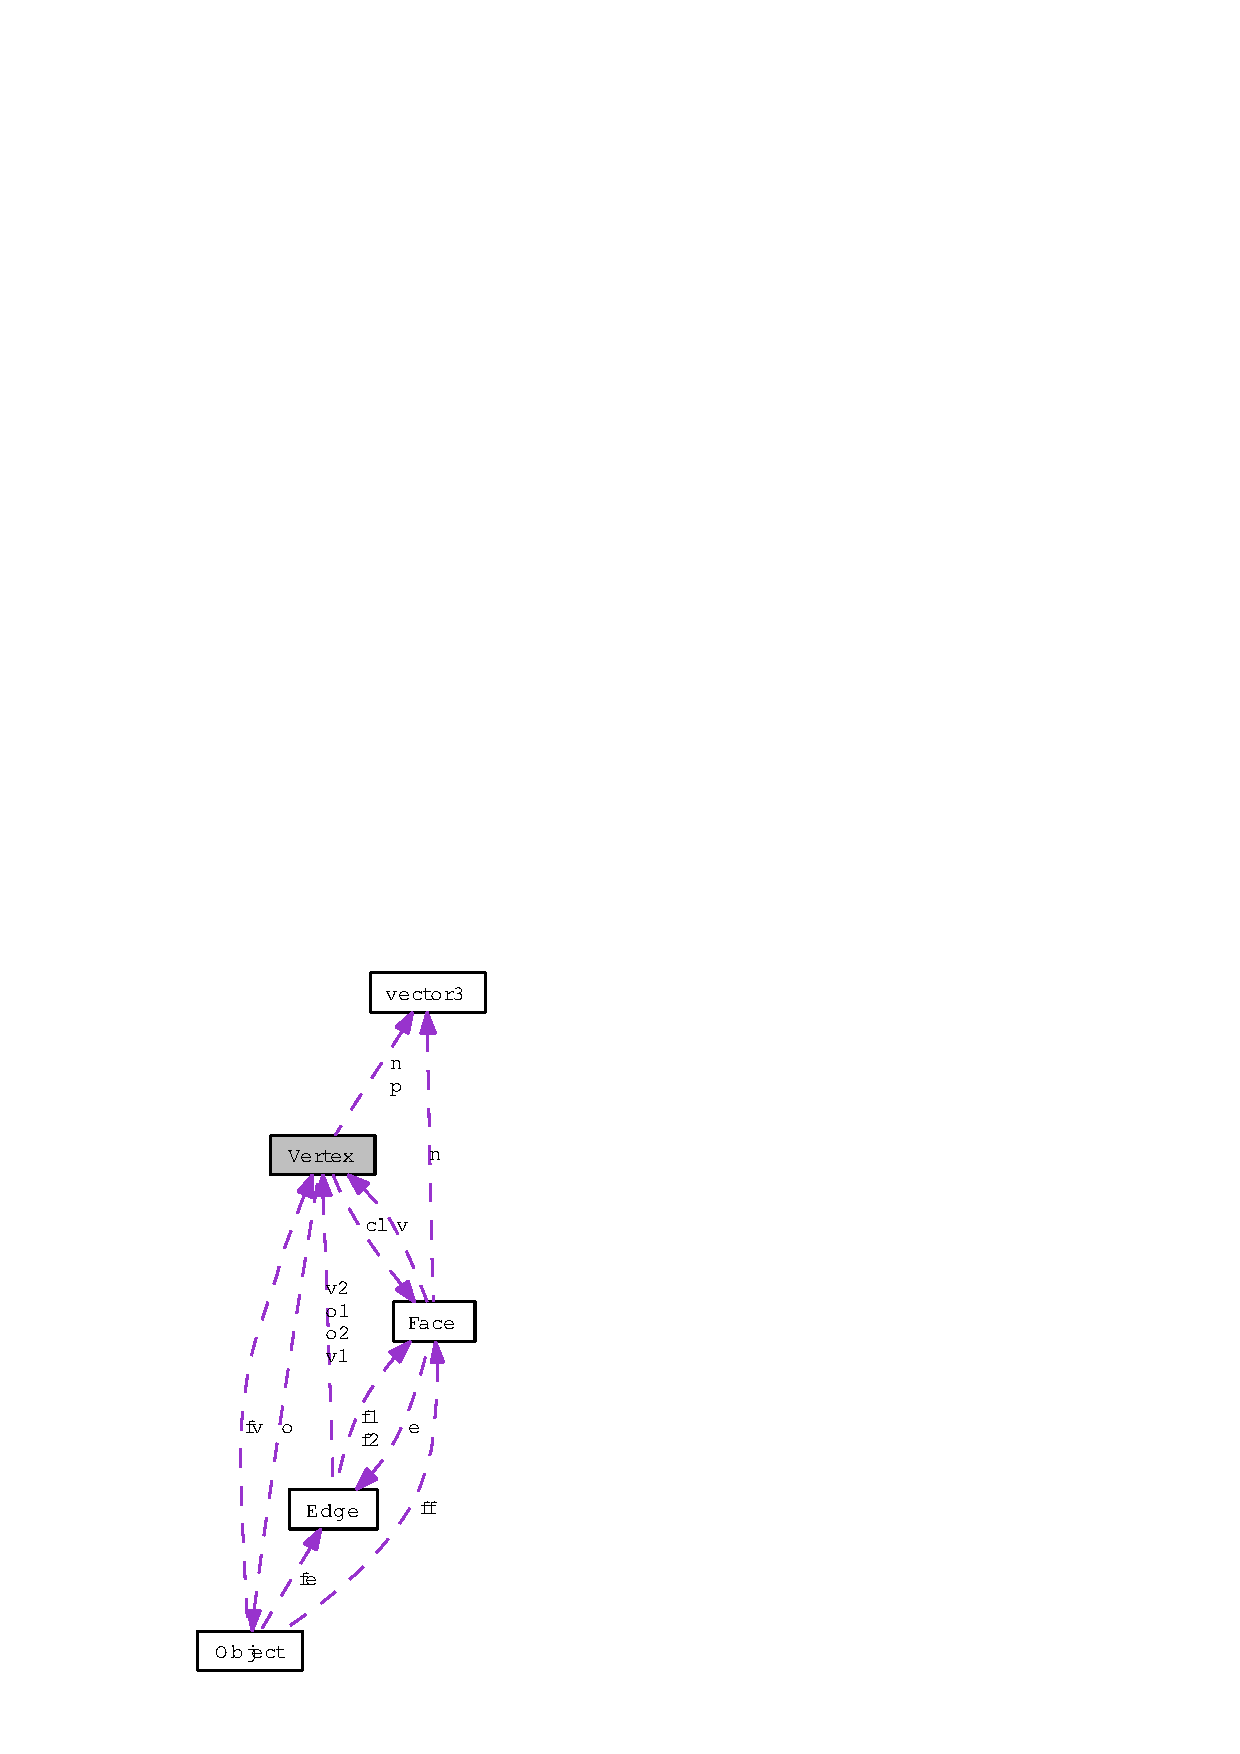
\includegraphics[width=122pt]{classVertex__coll__graph}
\end{center}
\end{figure}
\subsection*{Public Member Functions}
\begin{CompactItemize}
\item 
{\bf Vertex} (int const \&, double const \&x, double const \&y, double const \&z, {\bf Object} $\ast$const)
\item 
{\bf Vertex} ({\bf Vertex} const \&)
\item 
{\bf Vertex} \& {\bf operator=} ({\bf Vertex} const \&)
\item 
void {\bf print} (std::ostream \&) const
\item 
void {\bf print\-CP} (std::ostream \&) const
\item 
void {\bf set\-New\-Pos} ({\bf vector3} const $\ast$const)
\item 
void {\bf set\-Normal} (void)
\item 
void {\bf get\-Bounding\-Box} ({\bf vector3} \&, {\bf vector3} \&) const 
\item 
void {\bf update\-Adj\-Face\-Bounding\-Boxes} (void)
\item 
void {\bf define\-Local\-Region} ({\bf vector3} \&, {\bf vector3} \&)
\item 
void {\bf get\-Adj\-Vertices} ({\bf vec\_\-vp} \&) const
\item 
void {\bf get\-Adjacent\-Edges} ({\bf vec\_\-ep} \&) const
\item 
double {\bf get\-Sq\-Sep\-Dist} (void) const
\item 
double {\bf get\-Sq\-Virtual\-Disp} (double)
\item 
{\bf vector3} {\bf get\-New\-Pos} (double)
\item 
void {\bf record\-Adj\-Face\-Bounding\-Boxes} ({\bf hxa7241\_\-graphics::Vector3r} $\ast$const adjacent\_\-face\_\-lower, {\bf hxa7241\_\-graphics::Vector3r} $\ast$const adjacent\_\-face\_\-upper)
\item 
void {\bf get\-Total\-Force\-Energy} ({\bf vector3} \&) const
\item 
void {\bf get\-Adj\-Face\-Int\-Force} ({\bf vector3} \&) const
\item 
double {\bf get\-Ecw\-Force\-Energy} ({\bf vector3} \&, bool) const
\item 
double {\bf get\-Edge\-Stretch\-Force\-Energy} ({\bf vector3} \&, bool) const
\item 
double {\bf get\-Face\-Aspect\-Ratio\-Force\-Energy} ({\bf vector3} \&, bool) const
\item 
double {\bf get\-Edge\-Angle\-Force\-Energy} ({\bf vector3} \&, bool) const
\item 
{\bf Face} $\ast$ {\bf get\-Face\-Not\-Adj\-To\-Vertex} ({\bf Vertex} const $\ast$const) const 
\item 
void {\bf update\-Adjacent\-Face\-Normals} (void)
\item 
int {\bf get\-Last\-Refractory\-Iter} (void)
\item 
void {\bf set\-Last\-Refractory\-Iter} (int i)
\item 
void {\bf sort\-Adjacent\-Faces} (void)
\item 
{\bf vector3} {\bf get\-Normal} (void) const
\item 
int {\bf get\-Index} (void) const
\item 
int {\bf get\-Num\-Adj\-Faces} (void) const
\item 
bool {\bf face\-Is\-Adjacent} ({\bf Face} $\ast$face) const
\item 
bool {\bf is\-Match} (int const \&i, std::string const \&name) const
\item 
void {\bf add\-Adjacent\-Face} ({\bf Face} $\ast$face)
\item 
double const $\ast$ {\bf get\-Coord} (int const \&axis) const
\item 
{\bf Face} $\ast$ {\bf get\-Closest\-Face} (void)
\item 
void {\bf set\-Face} ({\bf Face} $\ast$const face)
\item 
{\bf vector3} const $\ast$ {\bf get\-Pos} (void) const
\item 
void {\bf set\-Pos} (double const \&x, double const \&y, double const \&z)
\item 
{\bf Object} const $\ast$ {\bf get\-Object} (void) const
\item 
{\bf fp\_\-cit} {\bf begin} (void) const
\item 
{\bf fp\_\-cit} {\bf end} (void) const
\end{CompactItemize}


\subsection{Constructor \& Destructor Documentation}
\index{Vertex@{Vertex}!Vertex@{Vertex}}
\index{Vertex@{Vertex}!Vertex@{Vertex}}
\subsubsection{\setlength{\rightskip}{0pt plus 5cm}Vertex::Vertex (int const \& {\em in}, double const \& {\em x}, double const \& {\em y}, double const \& {\em z}, {\bf Object} $\ast$ const {\em q})}\label{classVertex_6ebff1d17d628f435c2655520e57eb63}


Create new instance of \doxyref{Vertex}{p.}{classVertex} class.

\begin{Desc}
\item[Parameters:]
\begin{description}
\item[\mbox{$\leftarrow$} {\em line}]Single line from input mesh file. \item[\mbox{$\leftarrow$} {\em q}]Pointer to parent \doxyref{Object}{p.}{classObject}. \end{description}
\end{Desc}
\index{Vertex@{Vertex}!Vertex@{Vertex}}
\index{Vertex@{Vertex}!Vertex@{Vertex}}
\subsubsection{\setlength{\rightskip}{0pt plus 5cm}Vertex::Vertex ({\bf Vertex} const \&)}\label{classVertex_42156e0f7298c47e00f172a5f504028a}




\subsection{Member Function Documentation}
\index{Vertex@{Vertex}!operator=@{operator=}}
\index{operator=@{operator=}!Vertex@{Vertex}}
\subsubsection{\setlength{\rightskip}{0pt plus 5cm}{\bf Vertex} \& Vertex::operator= ({\bf Vertex} const \&)}\label{classVertex_d20da0d28fba10d6151cc8c5d756fff6}


\index{Vertex@{Vertex}!print@{print}}
\index{print@{print}!Vertex@{Vertex}}
\subsubsection{\setlength{\rightskip}{0pt plus 5cm}void Vertex::print (std::ostream \& {\em target}) const}\label{classVertex_ef328a4374db75403a25eb165c1b7066}


Print identifying vertex information to output stream.

\begin{Desc}
\item[Parameters:]
\begin{description}
\item[\mbox{$\leftarrow$} {\em target}]Pre-initialized output stream. \end{description}
\end{Desc}
\index{Vertex@{Vertex}!printCP@{printCP}}
\index{printCP@{printCP}!Vertex@{Vertex}}
\subsubsection{\setlength{\rightskip}{0pt plus 5cm}void Vertex::print\-CP (std::ostream \& {\em target}) const}\label{classVertex_277422e73e7ec49cec4239bfe0b98dbb}


Print to output stream the vertex position in DREa\-MM custom points format.

\begin{Desc}
\item[Parameters:]
\begin{description}
\item[\mbox{$\leftarrow$} {\em target}]Pre-initialized output stream. \end{description}
\end{Desc}
\index{Vertex@{Vertex}!setNewPos@{setNewPos}}
\index{setNewPos@{setNewPos}!Vertex@{Vertex}}
\subsubsection{\setlength{\rightskip}{0pt plus 5cm}void Vertex::set\-New\-Pos ({\bf vector3} const $\ast$ const {\em new\_\-position})}\label{classVertex_0e4d93fd1fd7e411c857492d0d7b328a}


Set new location for this vertex. \begin{Desc}
\item[Parameters:]
\begin{description}
\item[\mbox{$\leftarrow$} {\em new\_\-position}]New candidate position for this vertex. \end{description}
\end{Desc}
\index{Vertex@{Vertex}!setNormal@{setNormal}}
\index{setNormal@{setNormal}!Vertex@{Vertex}}
\subsubsection{\setlength{\rightskip}{0pt plus 5cm}void Vertex::set\-Normal (void)}\label{classVertex_338d57acc6a9e485afd0374fb8772fa2}


Calculate and store vertex normal vector computed as a weighted sum of adjacent face normals. \index{Vertex@{Vertex}!getBoundingBox@{getBoundingBox}}
\index{getBoundingBox@{getBoundingBox}!Vertex@{Vertex}}
\subsubsection{\setlength{\rightskip}{0pt plus 5cm}void Vertex::get\-Bounding\-Box ({\bf vector3} \& {\em lower}, {\bf vector3} \& {\em upper}) const}\label{classVertex_e968d8051fc4b83620920b6a149021cb}


Calculate and return vertex bounding box as bounding box of collection of adjacent faces. \begin{Desc}
\item[Parameters:]
\begin{description}
\item[\mbox{$\rightarrow$} {\em lower}]Lower corner of bounding box of collection of vertex adjacent faces. \item[\mbox{$\rightarrow$} {\em upper}]Upper corner of bounding box of collection of vertex adjacent faces. \end{description}
\end{Desc}
\index{Vertex@{Vertex}!updateAdjFaceBoundingBoxes@{updateAdjFaceBoundingBoxes}}
\index{updateAdjFaceBoundingBoxes@{updateAdjFaceBoundingBoxes}!Vertex@{Vertex}}
\subsubsection{\setlength{\rightskip}{0pt plus 5cm}void Vertex::update\-Adj\-Face\-Bounding\-Boxes (void)}\label{classVertex_1d9a88b8e7d1ffc4cc7b5679718bc307}


\index{Vertex@{Vertex}!defineLocalRegion@{defineLocalRegion}}
\index{defineLocalRegion@{defineLocalRegion}!Vertex@{Vertex}}
\subsubsection{\setlength{\rightskip}{0pt plus 5cm}void Vertex::define\-Local\-Region ({\bf vector3} \& {\em lower}, {\bf vector3} \& {\em upper})}\label{classVertex_f396f8cd8dcbac71a3db0c63fa39bf2e}


Calculate region around this vertex that is influenced by moving this vertex. \begin{Desc}
\item[Parameters:]
\begin{description}
\item[\mbox{$\rightarrow$} {\em lower}]Lower corner of local region. \item[\mbox{$\rightarrow$} {\em upper}]Upper corner of local region. \end{description}
\end{Desc}
\index{Vertex@{Vertex}!getAdjVertices@{getAdjVertices}}
\index{getAdjVertices@{getAdjVertices}!Vertex@{Vertex}}
\subsubsection{\setlength{\rightskip}{0pt plus 5cm}void Vertex::get\-Adj\-Vertices ({\bf vec\_\-vp} \& {\em adjacent\_\-vertices}) const}\label{classVertex_f5e00a98124f61e7c6877e8b843a50e2}


Collect and return vertices adjacent to this vertex. \begin{Desc}
\item[Parameters:]
\begin{description}
\item[\mbox{$\rightarrow$} {\em adjacent\_\-vertices}]Adjacent vertices of this vertex. \end{description}
\end{Desc}
\index{Vertex@{Vertex}!getAdjacentEdges@{getAdjacentEdges}}
\index{getAdjacentEdges@{getAdjacentEdges}!Vertex@{Vertex}}
\subsubsection{\setlength{\rightskip}{0pt plus 5cm}void Vertex::get\-Adjacent\-Edges ({\bf vec\_\-ep} \& {\em adjacent\_\-edges}) const}\label{classVertex_9698fd8ed0d0ecc74b08d25dfeb483d1}


Collect and return edges adjacent to this vertex. \begin{Desc}
\item[Parameters:]
\begin{description}
\item[\mbox{$\rightarrow$} {\em adjacent\_\-edges}]Adjacent edges of this vertex. \end{description}
\end{Desc}
\index{Vertex@{Vertex}!getSqSepDist@{getSqSepDist}}
\index{getSqSepDist@{getSqSepDist}!Vertex@{Vertex}}
\subsubsection{\setlength{\rightskip}{0pt plus 5cm}double Vertex::get\-Sq\-Sep\-Dist (void) const}\label{classVertex_08bdf63722a596fecada59dbc6a2ce67}


Calculare and return squared extracellular width of this vertex. \begin{Desc}
\item[Returns:]Squared extracellular width of this vertex. \end{Desc}
\index{Vertex@{Vertex}!getSqVirtualDisp@{getSqVirtualDisp}}
\index{getSqVirtualDisp@{getSqVirtualDisp}!Vertex@{Vertex}}
\subsubsection{\setlength{\rightskip}{0pt plus 5cm}double Vertex::get\-Sq\-Virtual\-Disp (double {\em gain})}\label{classVertex_d9fce6dd07b9f8053a0ee2f1dbfeba77}


Calculate and return the squared virtual displacement of this vertex. \begin{Desc}
\item[Parameters:]
\begin{description}
\item[\mbox{$\leftarrow$} {\em gain}]Proportionality constant between force and displacement. \end{description}
\end{Desc}
\begin{Desc}
\item[Returns:]Squared virtual displacement of this vertex. \end{Desc}
\index{Vertex@{Vertex}!getNewPos@{getNewPos}}
\index{getNewPos@{getNewPos}!Vertex@{Vertex}}
\subsubsection{\setlength{\rightskip}{0pt plus 5cm}{\bf vector3} Vertex::get\-New\-Pos (double {\em gain})}\label{classVertex_a7922650d655b0c69dbb3ba675021e59}


Calculate new vertex position. \begin{Desc}
\item[Parameters:]
\begin{description}
\item[\mbox{$\leftarrow$} {\em gain}]Proportionality between force and displacement. \end{description}
\end{Desc}
\begin{Desc}
\item[Returns:]New vertex location. \end{Desc}
\index{Vertex@{Vertex}!recordAdjFaceBoundingBoxes@{recordAdjFaceBoundingBoxes}}
\index{recordAdjFaceBoundingBoxes@{recordAdjFaceBoundingBoxes}!Vertex@{Vertex}}
\subsubsection{\setlength{\rightskip}{0pt plus 5cm}void Vertex::record\-Adj\-Face\-Bounding\-Boxes ({\bf hxa7241\_\-graphics::Vector3r} $\ast$const {\em adjacent\_\-face\_\-lower}, {\bf hxa7241\_\-graphics::Vector3r} $\ast$const {\em adjacent\_\-face\_\-upper})}\label{classVertex_8e996499ae0772ff3d6bcd5f92066859}


Record bounding box of each adjacent face of this vertex. \index{Vertex@{Vertex}!getTotalForceEnergy@{getTotalForceEnergy}}
\index{getTotalForceEnergy@{getTotalForceEnergy}!Vertex@{Vertex}}
\subsubsection{\setlength{\rightskip}{0pt plus 5cm}void Vertex::get\-Total\-Force\-Energy ({\bf vector3} \& {\em force}) const}\label{classVertex_c3a429d23891886ccb68c09967638c7e}


Calculate and return total force at this vertex, but energy is not computed. \begin{Desc}
\item[Parameters:]
\begin{description}
\item[\mbox{$\rightarrow$} {\em force}]Input force plus calculated force from all contributions. \end{description}
\end{Desc}
\index{Vertex@{Vertex}!getAdjFaceIntForce@{getAdjFaceIntForce}}
\index{getAdjFaceIntForce@{getAdjFaceIntForce}!Vertex@{Vertex}}
\subsubsection{\setlength{\rightskip}{0pt plus 5cm}void Vertex::get\-Adj\-Face\-Int\-Force ({\bf vector3} \& {\em force}) const}\label{classVertex_6ae08a26f3d0b1e812e02d62965e09da}


Calculate and return force and/or energy at this vertex due to adjacent face intersections. \begin{Desc}
\item[Parameters:]
\begin{description}
\item[\mbox{$\rightarrow$} {\em force}]Input force plus calculated adjacent face intersection contribution. \end{description}
\end{Desc}
\index{Vertex@{Vertex}!getEcwForceEnergy@{getEcwForceEnergy}}
\index{getEcwForceEnergy@{getEcwForceEnergy}!Vertex@{Vertex}}
\subsubsection{\setlength{\rightskip}{0pt plus 5cm}double Vertex::get\-Ecw\-Force\-Energy ({\bf vector3} \& {\em force}, bool {\em compute\_\-force}) const}\label{classVertex_9c451f0241ff1b35caf91373efb977c1}


Calculate and return the vertex force vector and energy due to the vertex extracellular width.

\begin{Desc}
\item[Parameters:]
\begin{description}
\item[\mbox{$\rightarrow$} {\em force}]The force vector due to the extracellular width is added to the input force. \item[\mbox{$\leftarrow$} {\em compute\_\-force}]If true, then compute force and energy; otherwise, compute only the energy. \end{description}
\end{Desc}
\index{Vertex@{Vertex}!getEdgeStretchForceEnergy@{getEdgeStretchForceEnergy}}
\index{getEdgeStretchForceEnergy@{getEdgeStretchForceEnergy}!Vertex@{Vertex}}
\subsubsection{\setlength{\rightskip}{0pt plus 5cm}double Vertex::get\-Edge\-Stretch\-Force\-Energy ({\bf vector3} \& {\em force}, bool {\em compute\_\-force}) const}\label{classVertex_2c0df9425320b0e9cb53f710b6d0591d}


Calculate and return force and/or energy at this vertex due to stretch of adjacent edges. \begin{Desc}
\item[Parameters:]
\begin{description}
\item[\mbox{$\rightarrow$} {\em force}]Input force plus calculated edge stretch contribution. \item[\mbox{$\leftarrow$} {\em compute\_\-force}]If true then compute force and energy; otherwise compute energy only. \end{description}
\end{Desc}
\begin{Desc}
\item[Returns:]Current energy stored in adjacent edge stretch. \end{Desc}
\index{Vertex@{Vertex}!getFaceAspectRatioForceEnergy@{getFaceAspectRatioForceEnergy}}
\index{getFaceAspectRatioForceEnergy@{getFaceAspectRatioForceEnergy}!Vertex@{Vertex}}
\subsubsection{\setlength{\rightskip}{0pt plus 5cm}double Vertex::get\-Face\-Aspect\-Ratio\-Force\-Energy ({\bf vector3} \& {\em force}, bool {\em compute\_\-force}) const}\label{classVertex_ae7528d909b3bc6f31a74713e5a520d5}


Calculate and return force and/or energy at this vertex due to aspect ratio of adjacent faces. \begin{Desc}
\item[Parameters:]
\begin{description}
\item[\mbox{$\rightarrow$} {\em force}]Input force plus calculated adjacent face contribution. \item[\mbox{$\leftarrow$} {\em compute\_\-force}]If true then compute force and energy; otherwise compute energy only. \end{description}
\end{Desc}
\begin{Desc}
\item[Returns:]Current energy stored in adjacent face aspect ratios. \end{Desc}
\index{Vertex@{Vertex}!getEdgeAngleForceEnergy@{getEdgeAngleForceEnergy}}
\index{getEdgeAngleForceEnergy@{getEdgeAngleForceEnergy}!Vertex@{Vertex}}
\subsubsection{\setlength{\rightskip}{0pt plus 5cm}double Vertex::get\-Edge\-Angle\-Force\-Energy ({\bf vector3} \& {\em force}, bool {\em compute\_\-force}) const}\label{classVertex_79b6556c8128e338848f4148126cf5c6}


Calculate and return force and/or energy at this vertex due to distribution of edge angles in adjacent faces of this vertex. \begin{Desc}
\item[Parameters:]
\begin{description}
\item[\mbox{$\rightarrow$} {\em force}]Input force plus calculated edge stretch contribution. \item[\mbox{$\leftarrow$} {\em compute\_\-force}]If true then compute force and energy; otherwise compute energy only. \end{description}
\end{Desc}
\begin{Desc}
\item[Returns:]Current energy stored in adjacent face edge angles. \end{Desc}
\index{Vertex@{Vertex}!getFaceNotAdjToVertex@{getFaceNotAdjToVertex}}
\index{getFaceNotAdjToVertex@{getFaceNotAdjToVertex}!Vertex@{Vertex}}
\subsubsection{\setlength{\rightskip}{0pt plus 5cm}{\bf Face} $\ast$ Vertex::get\-Face\-Not\-Adj\-To\-Vertex ({\bf Vertex} const $\ast$ const {\em avoided\_\-vertex}) const}\label{classVertex_3c4e5c26165558d81dc32ea2876e87f6}


Find and return an adjacent face to this vertex that does not contain the input vertex. \begin{Desc}
\item[Parameters:]
\begin{description}
\item[\mbox{$\leftarrow$} {\em avoided\_\-vertex}]\doxyref{Vertex}{p.}{classVertex} that adjacent face must not reference. \end{description}
\end{Desc}
\begin{Desc}
\item[Returns:]Pointer to adjacent face of this vertex. \end{Desc}
\index{Vertex@{Vertex}!updateAdjacentFaceNormals@{updateAdjacentFaceNormals}}
\index{updateAdjacentFaceNormals@{updateAdjacentFaceNormals}!Vertex@{Vertex}}
\subsubsection{\setlength{\rightskip}{0pt plus 5cm}void Vertex::update\-Adjacent\-Face\-Normals (void)}\label{classVertex_b8f027f61bdbecdf10135be8b54b9a77}


Recalculate normal vectors of faces adjacent to this vertex. \index{Vertex@{Vertex}!getLastRefractoryIter@{getLastRefractoryIter}}
\index{getLastRefractoryIter@{getLastRefractoryIter}!Vertex@{Vertex}}
\subsubsection{\setlength{\rightskip}{0pt plus 5cm}int Vertex::get\-Last\-Refractory\-Iter (void)\hspace{0.3cm}{\tt  [inline]}}\label{classVertex_f2136c527a0a5881fc34399ed8ec6459}


\index{Vertex@{Vertex}!setLastRefractoryIter@{setLastRefractoryIter}}
\index{setLastRefractoryIter@{setLastRefractoryIter}!Vertex@{Vertex}}
\subsubsection{\setlength{\rightskip}{0pt plus 5cm}void Vertex::set\-Last\-Refractory\-Iter (int {\em i})\hspace{0.3cm}{\tt  [inline]}}\label{classVertex_8b77fc93f9f23b3660a87b7180780c92}


\index{Vertex@{Vertex}!sortAdjacentFaces@{sortAdjacentFaces}}
\index{sortAdjacentFaces@{sortAdjacentFaces}!Vertex@{Vertex}}
\subsubsection{\setlength{\rightskip}{0pt plus 5cm}void Vertex::sort\-Adjacent\-Faces (void)\hspace{0.3cm}{\tt  [inline]}}\label{classVertex_33ec689fc3b54c151218b450a36c9440}


Sort stored adjacent faces to this vertex by face pointer. \index{Vertex@{Vertex}!getNormal@{getNormal}}
\index{getNormal@{getNormal}!Vertex@{Vertex}}
\subsubsection{\setlength{\rightskip}{0pt plus 5cm}{\bf vector3} Vertex::get\-Normal (void) const\hspace{0.3cm}{\tt  [inline]}}\label{classVertex_a59ca2c107b5ebf845465cde1e27b509}


Get stored vertex normal vector.

\begin{Desc}
\item[Returns:]\doxyref{Vertex}{p.}{classVertex} normal vector. Note vector length is not necessarily of unit length. \end{Desc}
\index{Vertex@{Vertex}!getIndex@{getIndex}}
\index{getIndex@{getIndex}!Vertex@{Vertex}}
\subsubsection{\setlength{\rightskip}{0pt plus 5cm}int Vertex::get\-Index (void) const\hspace{0.3cm}{\tt  [inline]}}\label{classVertex_0487c340a3a1559f4a8e45d8a7b0f9e2}


Return the index of vertex as recorded from input file.

\begin{Desc}
\item[Returns:]\doxyref{Vertex}{p.}{classVertex} index. \end{Desc}
\index{Vertex@{Vertex}!getNumAdjFaces@{getNumAdjFaces}}
\index{getNumAdjFaces@{getNumAdjFaces}!Vertex@{Vertex}}
\subsubsection{\setlength{\rightskip}{0pt plus 5cm}int Vertex::get\-Num\-Adj\-Faces (void) const\hspace{0.3cm}{\tt  [inline]}}\label{classVertex_b01da7ba35653cce77dfd96d3ec04872}


Calculate and return the number of stored adjacent faces to this vertex. \begin{Desc}
\item[Returns:]Number of stored adjacent faces to this vertex. \end{Desc}
\index{Vertex@{Vertex}!faceIsAdjacent@{faceIsAdjacent}}
\index{faceIsAdjacent@{faceIsAdjacent}!Vertex@{Vertex}}
\subsubsection{\setlength{\rightskip}{0pt plus 5cm}bool Vertex::face\-Is\-Adjacent ({\bf Face} $\ast$ {\em face}) const\hspace{0.3cm}{\tt  [inline]}}\label{classVertex_5d17892f8483a0d7c168a47c1a561557}


Determine if input face is adjacent to this vertex. \begin{Desc}
\item[Parameters:]
\begin{description}
\item[\mbox{$\leftarrow$} {\em face}]\doxyref{Face}{p.}{classFace} of interest. \end{description}
\end{Desc}
\begin{Desc}
\item[Returns:]True if input face is found among stored adjcent faces of this vertes; false otherwise. \end{Desc}
\index{Vertex@{Vertex}!isMatch@{isMatch}}
\index{isMatch@{isMatch}!Vertex@{Vertex}}
\subsubsection{\setlength{\rightskip}{0pt plus 5cm}bool Vertex::is\-Match (int const \& {\em i}, std::string const \& {\em name}) const\hspace{0.3cm}{\tt  [inline]}}\label{classVertex_bb086dcb3e4f4fd2098ffdba5ac8c019}


Compare input vertex index and object name to this vertex's index and object name. \begin{Desc}
\item[Parameters:]
\begin{description}
\item[\mbox{$\leftarrow$} {\em i}]Input vertex index. \item[\mbox{$\leftarrow$} {\em name}]Input vertex parent object name. \end{description}
\end{Desc}
\begin{Desc}
\item[Returns:]True if indices and names match; false otherwise. \end{Desc}
\index{Vertex@{Vertex}!addAdjacentFace@{addAdjacentFace}}
\index{addAdjacentFace@{addAdjacentFace}!Vertex@{Vertex}}
\subsubsection{\setlength{\rightskip}{0pt plus 5cm}void Vertex::add\-Adjacent\-Face ({\bf Face} $\ast$ {\em face})\hspace{0.3cm}{\tt  [inline]}}\label{classVertex_2f7d68842e13eaf8423e0a00d23beb04}


Record input face as adjacent to this vertex. \begin{Desc}
\item[Parameters:]
\begin{description}
\item[\mbox{$\leftarrow$} {\em face}]New adjacent face to this vertex. \end{description}
\end{Desc}
\index{Vertex@{Vertex}!getCoord@{getCoord}}
\index{getCoord@{getCoord}!Vertex@{Vertex}}
\subsubsection{\setlength{\rightskip}{0pt plus 5cm}double const$\ast$ Vertex::get\-Coord (int const \& {\em axis}) const\hspace{0.3cm}{\tt  [inline]}}\label{classVertex_a9d753c6db6816f5a6d649dc06b2bab4}


Retrieve one coordinate of position of this vertex. \begin{Desc}
\item[Parameters:]
\begin{description}
\item[\mbox{$\leftarrow$} {\em axis}]Axis of interest (0,1,2==x,y,z axis respectively). \end{description}
\end{Desc}
\begin{Desc}
\item[Returns:]The position coordinate of this vertex with index equal to axis. \end{Desc}
\index{Vertex@{Vertex}!getClosestFace@{getClosestFace}}
\index{getClosestFace@{getClosestFace}!Vertex@{Vertex}}
\subsubsection{\setlength{\rightskip}{0pt plus 5cm}{\bf Face}$\ast$ Vertex::get\-Closest\-Face (void)\hspace{0.3cm}{\tt  [inline]}}\label{classVertex_d6c234ee24e36b3d350a472769adcef4}


Retrieve the stored face on which the closest point to this vertex should lie. \begin{Desc}
\item[Returns:]Stored closest face pointer. \end{Desc}
\index{Vertex@{Vertex}!setFace@{setFace}}
\index{setFace@{setFace}!Vertex@{Vertex}}
\subsubsection{\setlength{\rightskip}{0pt plus 5cm}void Vertex::set\-Face ({\bf Face} $\ast$const  {\em face})\hspace{0.3cm}{\tt  [inline]}}\label{classVertex_d18dc62be3daf37e8796f557b93acc25}


Record the stored face on which the closest point to this vertex should lie. \begin{Desc}
\item[Parameters:]
\begin{description}
\item[\mbox{$\leftarrow$} {\em face}]Pointer to closet face to this vertex.. \end{description}
\end{Desc}
\index{Vertex@{Vertex}!getPos@{getPos}}
\index{getPos@{getPos}!Vertex@{Vertex}}
\subsubsection{\setlength{\rightskip}{0pt plus 5cm}{\bf vector3} const$\ast$ Vertex::get\-Pos (void) const\hspace{0.3cm}{\tt  [inline]}}\label{classVertex_6806afb3595d95814da949e54feb9105}


Retrieve the current position of this vertex. \begin{Desc}
\item[Returns:]Pointer to this vertex. \end{Desc}
\index{Vertex@{Vertex}!setPos@{setPos}}
\index{setPos@{setPos}!Vertex@{Vertex}}
\subsubsection{\setlength{\rightskip}{0pt plus 5cm}void Vertex::set\-Pos (double const \& {\em x}, double const \& {\em y}, double const \& {\em z})\hspace{0.3cm}{\tt  [inline]}}\label{classVertex_01f45c280d33aa0ccb6037bdb9c02583}


Set the position of this vertex. \begin{Desc}
\item[Parameters:]
\begin{description}
\item[\mbox{$\leftarrow$} {\em x}]X coordinate. \item[\mbox{$\leftarrow$} {\em y}]Y coordinate. \item[\mbox{$\leftarrow$} {\em z}]Z coordinate. \end{description}
\end{Desc}
\index{Vertex@{Vertex}!getObject@{getObject}}
\index{getObject@{getObject}!Vertex@{Vertex}}
\subsubsection{\setlength{\rightskip}{0pt plus 5cm}{\bf Object} const$\ast$ Vertex::get\-Object (void) const\hspace{0.3cm}{\tt  [inline]}}\label{classVertex_3f1a260d589727b4deddac476429e37b}


Retrieve a pointer to the parent \doxyref{Object}{p.}{classObject} of this vertex. \begin{Desc}
\item[Returns:]Pointer to parent object of this vertex. \end{Desc}
\index{Vertex@{Vertex}!begin@{begin}}
\index{begin@{begin}!Vertex@{Vertex}}
\subsubsection{\setlength{\rightskip}{0pt plus 5cm}{\bf fp\_\-cit} Vertex::begin (void) const\hspace{0.3cm}{\tt  [inline]}}\label{classVertex_7ebc259c68c71408ecc67662d64e9ec0}


Get an iterator pointing to the first in the collection of adjacent faces to this vertex. \begin{Desc}
\item[Returns:]Iterator pointing to the first adjacent face. \end{Desc}
\index{Vertex@{Vertex}!end@{end}}
\index{end@{end}!Vertex@{Vertex}}
\subsubsection{\setlength{\rightskip}{0pt plus 5cm}{\bf fp\_\-cit} Vertex::end (void) const\hspace{0.3cm}{\tt  [inline]}}\label{classVertex_4bb81e4284f35a668f19495419a23abb}


Get an iterator pointing to one past the last in the collection of adjacent faces to this vertex. \begin{Desc}
\item[Returns:]Iterator pointing to one past the last adjacent face. \end{Desc}


The documentation for this class was generated from the following files:\begin{CompactItemize}
\item 
{\bf vertex.h}\item 
{\bf vertex.cc}\end{CompactItemize}

\section{Vertex\_\-Schedule Class Reference}
\label{classVertex__Schedule}\index{Vertex_Schedule@{Vertex\_\-Schedule}}
{\tt \#include $<$vertex\_\-schedule.h$>$}

Collaboration diagram for Vertex\_\-Schedule:\begin{figure}[H]
\begin{center}
\leavevmode
\includegraphics[width=210pt]{classVertex__Schedule__coll__graph}
\end{center}
\end{figure}
\subsection*{Public Member Functions}
\begin{CompactItemize}
\item 
void {\bf calculate\-Move\-Location} ({\bf Vertex} $\ast$const)
\item 
void {\bf collect\-Vertices\-To\-Move\-Next} (const int \&)
\item 
void {\bf read\-Vertex\-Sequence} (const char $\ast$filename)
\item 
{\bf vp\_\-cit} {\bf begin\-Vset} (void) const
\item 
{\bf vp\_\-cit} {\bf end\-Vset} (void) const
\item 
void {\bf increment\-Num\-Moved\-Verts\-Group} (void)
\item 
{\bf vector3} const $\ast$ {\bf get\-Vertex\-Destination} (void) const
\item 
{\bf Vertex} $\ast$ {\bf get\-Current\-Vertex} (void) const
\item 
{\bf Vertex} $\ast$ {\bf get\-Seed\-Vertex} (void) const
\item 
int {\bf get\-Num\-Moved\-Verts\-Group} (void) const
\item 
void {\bf set\-Num\-Moved\-Verts\-Group} (int const \&init\_\-value)
\item 
bool {\bf no\-More\-Vertices\-To\-Move} (void) const
\item 
int {\bf get\-Reference\-Count\-Moved\-Verts} (void) const
\item 
bool {\bf no\-Set\-Vertices\-Moved} (void) const
\end{CompactItemize}
\subsection*{Static Public Member Functions}
\begin{CompactItemize}
\item 
static {\bf Vertex\_\-Schedule} \& {\bf instance} (void)
\end{CompactItemize}


\subsection{Member Function Documentation}
\index{Vertex_Schedule@{Vertex\_\-Schedule}!instance@{instance}}
\index{instance@{instance}!Vertex_Schedule@{Vertex\_\-Schedule}}
\subsubsection{\setlength{\rightskip}{0pt plus 5cm}{\bf Vertex\_\-Schedule} \& Vertex\_\-Schedule::instance (void)\hspace{0.3cm}{\tt  [static]}}\label{classVertex__Schedule_73029813663350a537c863c67976bcb6}


\index{Vertex_Schedule@{Vertex\_\-Schedule}!calculateMoveLocation@{calculateMoveLocation}}
\index{calculateMoveLocation@{calculateMoveLocation}!Vertex_Schedule@{Vertex\_\-Schedule}}
\subsubsection{\setlength{\rightskip}{0pt plus 5cm}void Vertex\_\-Schedule::calculate\-Move\-Location ({\bf Vertex} $\ast$ const {\em v})}\label{classVertex__Schedule_7132091b660efa36c5eb3e1dd0934967}


Calculate and record move location of input vertex. \begin{Desc}
\item[Parameters:]
\begin{description}
\item[\mbox{$\leftarrow$} {\em v}]\doxyref{Vertex}{p.}{classVertex} attempting a move. \end{description}
\end{Desc}
\index{Vertex_Schedule@{Vertex\_\-Schedule}!collectVerticesToMoveNext@{collectVerticesToMoveNext}}
\index{collectVerticesToMoveNext@{collectVerticesToMoveNext}!Vertex_Schedule@{Vertex\_\-Schedule}}
\subsubsection{\setlength{\rightskip}{0pt plus 5cm}void Vertex\_\-Schedule::collect\-Vertices\-To\-Move\-Next (const int \& {\em group})}\label{classVertex__Schedule_c3621ca9569e5a38e5daffdad2cb0775}


Identify and record a collection of vertices to move next. \index{Vertex_Schedule@{Vertex\_\-Schedule}!readVertexSequence@{readVertexSequence}}
\index{readVertexSequence@{readVertexSequence}!Vertex_Schedule@{Vertex\_\-Schedule}}
\subsubsection{\setlength{\rightskip}{0pt plus 5cm}void Vertex\_\-Schedule::read\-Vertex\-Sequence (const char $\ast$ {\em filename})}\label{classVertex__Schedule_dec602593611f7ebea28143926679b94}


Process vertex move sequence data. \begin{Desc}
\item[Parameters:]
\begin{description}
\item[\mbox{$\leftarrow$} {\em filename}]File containing a list of vertices to be moved in order. \end{description}
\end{Desc}
\index{Vertex_Schedule@{Vertex\_\-Schedule}!beginVset@{beginVset}}
\index{beginVset@{beginVset}!Vertex_Schedule@{Vertex\_\-Schedule}}
\subsubsection{\setlength{\rightskip}{0pt plus 5cm}{\bf vp\_\-cit} Vertex\_\-Schedule::begin\-Vset (void) const\hspace{0.3cm}{\tt  [inline]}}\label{classVertex__Schedule_768f889614599162ae3d70981e791d6a}


Get an iterator pointing to the first in the collection of vertices to move next. \begin{Desc}
\item[Returns:]Iterator pointing to the first vertex to move next. \end{Desc}
\index{Vertex_Schedule@{Vertex\_\-Schedule}!endVset@{endVset}}
\index{endVset@{endVset}!Vertex_Schedule@{Vertex\_\-Schedule}}
\subsubsection{\setlength{\rightskip}{0pt plus 5cm}{\bf vp\_\-cit} Vertex\_\-Schedule::end\-Vset (void) const\hspace{0.3cm}{\tt  [inline]}}\label{classVertex__Schedule_e2ef596b2c4a47b69be3c3f822d7bcfc}


Get an iterator pointing to one past the last in the collection of vertices to move next. \begin{Desc}
\item[Returns:]Iterator pointing to one past the last vertex to move next. \end{Desc}
\index{Vertex_Schedule@{Vertex\_\-Schedule}!incrementNumMovedVertsGroup@{incrementNumMovedVertsGroup}}
\index{incrementNumMovedVertsGroup@{incrementNumMovedVertsGroup}!Vertex_Schedule@{Vertex\_\-Schedule}}
\subsubsection{\setlength{\rightskip}{0pt plus 5cm}void Vertex\_\-Schedule::increment\-Num\-Moved\-Verts\-Group (void)\hspace{0.3cm}{\tt  [inline]}}\label{classVertex__Schedule_8bf86d52437824c1b78ca0f5ed9e5c0c}


Increment the number of moved vertices in group. \index{Vertex_Schedule@{Vertex\_\-Schedule}!getVertexDestination@{getVertexDestination}}
\index{getVertexDestination@{getVertexDestination}!Vertex_Schedule@{Vertex\_\-Schedule}}
\subsubsection{\setlength{\rightskip}{0pt plus 5cm}{\bf vector3} const$\ast$ Vertex\_\-Schedule::get\-Vertex\-Destination (void) const\hspace{0.3cm}{\tt  [inline]}}\label{classVertex__Schedule_3ae6a55e230276a631d20949138dd9c4}


Retrieve the location to which current vertex is attempting to move. \begin{Desc}
\item[Returns:]Recorded move location of current vertex. \end{Desc}
\index{Vertex_Schedule@{Vertex\_\-Schedule}!getCurrentVertex@{getCurrentVertex}}
\index{getCurrentVertex@{getCurrentVertex}!Vertex_Schedule@{Vertex\_\-Schedule}}
\subsubsection{\setlength{\rightskip}{0pt plus 5cm}{\bf Vertex}$\ast$ Vertex\_\-Schedule::get\-Current\-Vertex (void) const\hspace{0.3cm}{\tt  [inline]}}\label{classVertex__Schedule_eece2662bcd81cbf2fdfa4d1c6d53410}


Retrieve vertex attempting to move now. \begin{Desc}
\item[Returns:]Pointer to vertex attempting to move now. \end{Desc}
\index{Vertex_Schedule@{Vertex\_\-Schedule}!getSeedVertex@{getSeedVertex}}
\index{getSeedVertex@{getSeedVertex}!Vertex_Schedule@{Vertex\_\-Schedule}}
\subsubsection{\setlength{\rightskip}{0pt plus 5cm}{\bf Vertex}$\ast$ Vertex\_\-Schedule::get\-Seed\-Vertex (void) const\hspace{0.3cm}{\tt  [inline]}}\label{classVertex__Schedule_4935f3472cc6c77042c7032a063b5de7}


Retrieve pointer to seed vertex of collection of vertices to move. \begin{Desc}
\item[Returns:]Pointer to seed vertex. \end{Desc}
\index{Vertex_Schedule@{Vertex\_\-Schedule}!getNumMovedVertsGroup@{getNumMovedVertsGroup}}
\index{getNumMovedVertsGroup@{getNumMovedVertsGroup}!Vertex_Schedule@{Vertex\_\-Schedule}}
\subsubsection{\setlength{\rightskip}{0pt plus 5cm}int Vertex\_\-Schedule::get\-Num\-Moved\-Verts\-Group (void) const\hspace{0.3cm}{\tt  [inline]}}\label{classVertex__Schedule_802d1b6d13c9f3d82325f80590f46e03}


Retrieve the number of vertices moved so far in this group. \begin{Desc}
\item[Returns:]The number of vertices moved so far in this group. \end{Desc}
\index{Vertex_Schedule@{Vertex\_\-Schedule}!setNumMovedVertsGroup@{setNumMovedVertsGroup}}
\index{setNumMovedVertsGroup@{setNumMovedVertsGroup}!Vertex_Schedule@{Vertex\_\-Schedule}}
\subsubsection{\setlength{\rightskip}{0pt plus 5cm}void Vertex\_\-Schedule::set\-Num\-Moved\-Verts\-Group (int const \& {\em init\_\-value})\hspace{0.3cm}{\tt  [inline]}}\label{classVertex__Schedule_9588d4a7a1da405bc8bb5c533b337c32}


Initialize number of moved vertices in group. \begin{Desc}
\item[Parameters:]
\begin{description}
\item[\mbox{$\leftarrow$} {\em init\_\-value}]Initial value of number of moved vertices. \end{description}
\end{Desc}
\index{Vertex_Schedule@{Vertex\_\-Schedule}!noMoreVerticesToMove@{noMoreVerticesToMove}}
\index{noMoreVerticesToMove@{noMoreVerticesToMove}!Vertex_Schedule@{Vertex\_\-Schedule}}
\subsubsection{\setlength{\rightskip}{0pt plus 5cm}bool Vertex\_\-Schedule::no\-More\-Vertices\-To\-Move (void) const\hspace{0.3cm}{\tt  [inline]}}\label{classVertex__Schedule_bfe2aad2c1fc3178288702906940e764}


Check if more vertices in collection to move. \begin{Desc}
\item[Returns:]True if no more vertices to move; false otherwise. \end{Desc}
\index{Vertex_Schedule@{Vertex\_\-Schedule}!getReferenceCountMovedVerts@{getReferenceCountMovedVerts}}
\index{getReferenceCountMovedVerts@{getReferenceCountMovedVerts}!Vertex_Schedule@{Vertex\_\-Schedule}}
\subsubsection{\setlength{\rightskip}{0pt plus 5cm}int Vertex\_\-Schedule::get\-Reference\-Count\-Moved\-Verts (void) const\hspace{0.3cm}{\tt  [inline]}}\label{classVertex__Schedule_1710822552824e6934e207010456519f}


Retrieve the number of moved vertices in group at start of last set of moved vertices. \begin{Desc}
\item[Returns:]Reference count of moved vertices in group. \end{Desc}
\index{Vertex_Schedule@{Vertex\_\-Schedule}!noSetVerticesMoved@{noSetVerticesMoved}}
\index{noSetVerticesMoved@{noSetVerticesMoved}!Vertex_Schedule@{Vertex\_\-Schedule}}
\subsubsection{\setlength{\rightskip}{0pt plus 5cm}bool Vertex\_\-Schedule::no\-Set\-Vertices\-Moved (void) const\hspace{0.3cm}{\tt  [inline]}}\label{classVertex__Schedule_4d1f64b9e725eab1b672c545cba5e2b7}


Determine if any vertices were moved from last set of move candidates. \begin{Desc}
\item[Returns:]True if no vertices were moved; false otherwise. \end{Desc}


The documentation for this class was generated from the following files:\begin{CompactItemize}
\item 
{\bf vertex\_\-schedule.h}\item 
{\bf vertex\_\-schedule.cc}\end{CompactItemize}

\section{Virtual\_\-Disp Class Reference}
\label{classVirtual__Disp}\index{Virtual_Disp@{Virtual\_\-Disp}}
{\tt \#include $<$virtual\_\-disp.h$>$}

Collaboration diagram for Virtual\_\-Disp:\begin{figure}[H]
\begin{center}
\leavevmode
\includegraphics[width=93pt]{classVirtual__Disp__coll__graph}
\end{center}
\end{figure}
\subsection*{Public Member Functions}
\begin{CompactItemize}
\item 
void {\bf build\-Virt\-Disp\-Map\-Complement} (void)
\item 
bool {\bf find\-Virt\-Disp\-To\-Vert\-Assoc} ({\bf Vertex} $\ast$const, float const \&, {\bf tv\_\-it} \&)
\item 
void {\bf build\-Virt\-Disp\-Map} (const int \&)
\item 
void {\bf set\-Virtual\-Disp} ({\bf Vertex} $\ast$const, float const \&)
\item 
void {\bf update\-Virtual\-Disp} ({\bf Vertex} $\ast$const, bool const, float const \&)
\item 
void {\bf remove\-Virt\-Disp\-To\-Vert\-Assoc} ({\bf Vertex} $\ast$const, float const \&)
\item 
bool {\bf get\-Vert\-And\-Rank} ({\bf Vertex} $\ast$const, {\bf tv\_\-it} \&, int \&)
\item 
void {\bf reset\-For\-New\-Group} (const int \&)
\item 
void {\bf remove\-Vert\-From\-All\-Maps} ({\bf Vertex} $\ast$)
\item 
void {\bf validate\-Virt\-Disp\-Map\-Complement} (void)
\item 
void {\bf validate\-Virt\-Disp\-Map2} (void)
\item 
void {\bf validate\-Virt\-Disp\-Map} (void) const
\item 
void {\bf add\-Ad\-To\-Seed\-Ad} (const int \&count, double ad)
\item 
void {\bf add\-Vd\-To\-Seed\-Vd} (const int \&count)
\item 
{\bf s\_\-cit} {\bf begin\-Seed\-Act\-Disp} (void)
\item 
{\bf s\_\-cit} {\bf end\-Seed\-Act\-Disp} (void)
\item 
{\bf s\_\-cit} {\bf begin\-Seed\-Virt\-Disp} (void)
\item 
{\bf s\_\-cit} {\bf end\-Seed\-Virt\-Disp} (void)
\item 
{\bf tv\_\-crit} {\bf get\-Seed} (void)
\item 
int {\bf get\-Num\-Verts\-In\-Virt\-Disp\-Map} (void)
\item 
void {\bf advance\-Seed\-To\-Next\-Largest\-Vert} (void)
\item 
void {\bf reset\-Seed\-To\-Largest\-Vert} (void)
\item 
{\bf tv\_\-cit} {\bf begin\-Virt\-Disp\-Map} (void)
\item 
{\bf tv\_\-crit} {\bf rend\-Virt\-Disp\-Map} (void)
\item 
{\bf tv\_\-cit} {\bf end\-Virt\-Disp\-Map} (void)
\end{CompactItemize}
\subsection*{Static Public Member Functions}
\begin{CompactItemize}
\item 
static {\bf Virtual\_\-Disp} \& {\bf instance} (void)
\end{CompactItemize}


\subsection{Member Function Documentation}
\index{Virtual_Disp@{Virtual\_\-Disp}!instance@{instance}}
\index{instance@{instance}!Virtual_Disp@{Virtual\_\-Disp}}
\subsubsection{\setlength{\rightskip}{0pt plus 5cm}{\bf Virtual\_\-Disp} \& Virtual\_\-Disp::instance (void)\hspace{0.3cm}{\tt  [static]}}\label{classVirtual__Disp_cfa60cce91fdade84b2030b81d70ad22}


\index{Virtual_Disp@{Virtual\_\-Disp}!buildVirtDispMapComplement@{buildVirtDispMapComplement}}
\index{buildVirtDispMapComplement@{buildVirtDispMapComplement}!Virtual_Disp@{Virtual\_\-Disp}}
\subsubsection{\setlength{\rightskip}{0pt plus 5cm}void Virtual\_\-Disp::build\-Virt\-Disp\-Map\-Complement (void)}\label{classVirtual__Disp_abf9ca3e97dd2046dd148e6d6affe4b2}


Build v\_\-to\_\-vd2, the complement map of vd2\_\-to\_\-v. \index{Virtual_Disp@{Virtual\_\-Disp}!findVirtDispToVertAssoc@{findVirtDispToVertAssoc}}
\index{findVirtDispToVertAssoc@{findVirtDispToVertAssoc}!Virtual_Disp@{Virtual\_\-Disp}}
\subsubsection{\setlength{\rightskip}{0pt plus 5cm}bool Virtual\_\-Disp::find\-Virt\-Disp\-To\-Vert\-Assoc ({\bf Vertex} $\ast$ const {\em v}, float const \& {\em sqd\_\-vd}, {\bf tv\_\-it} \& {\em match})}\label{classVirtual__Disp_e04623758bf027aa71daa89499cd3d80}


Find and return element in vd2\_\-to\_\-v that matches input vertex and squared virtual displacement. \begin{Desc}
\item[Parameters:]
\begin{description}
\item[\mbox{$\leftarrow$} {\em v}]\doxyref{Vertex}{p.}{classVertex} of interest. \item[\mbox{$\leftarrow$} {\em sqd\_\-vd}]Squared virtual displacement of vertex. \item[\mbox{$\rightarrow$} {\em match}]Iterator to matching vd2\_\-to\_\-v element, if found; \end{description}
\end{Desc}
\begin{Desc}
\item[Returns:]True if match found; false otherwise. \end{Desc}
\index{Virtual_Disp@{Virtual\_\-Disp}!buildVirtDispMap@{buildVirtDispMap}}
\index{buildVirtDispMap@{buildVirtDispMap}!Virtual_Disp@{Virtual\_\-Disp}}
\subsubsection{\setlength{\rightskip}{0pt plus 5cm}void Virtual\_\-Disp::build\-Virt\-Disp\-Map (const int \& {\em group})}\label{classVirtual__Disp_32764f06734a84946095b7703579e24f}


Build vd2\_\-to\_\-v (which maps squared virtual dispacement to vertex pointer). \index{Virtual_Disp@{Virtual\_\-Disp}!setVirtualDisp@{setVirtualDisp}}
\index{setVirtualDisp@{setVirtualDisp}!Virtual_Disp@{Virtual\_\-Disp}}
\subsubsection{\setlength{\rightskip}{0pt plus 5cm}void Virtual\_\-Disp::set\-Virtual\-Disp ({\bf Vertex} $\ast$ const {\em v}, float const \& {\em sqd\_\-vd})}\label{classVirtual__Disp_ac2a04238e5a737cf6c36541ad6792a2}


Record association between input vertex and squared virtual displacement, removing any previous associations. \begin{Desc}
\item[Parameters:]
\begin{description}
\item[\mbox{$\leftarrow$} {\em v}]\doxyref{Vertex}{p.}{classVertex} of interest. \item[\mbox{$\leftarrow$} {\em sqd\_\-vd}]Squared virtual displacement of vertex. \end{description}
\end{Desc}
\index{Virtual_Disp@{Virtual\_\-Disp}!updateVirtualDisp@{updateVirtualDisp}}
\index{updateVirtualDisp@{updateVirtualDisp}!Virtual_Disp@{Virtual\_\-Disp}}
\subsubsection{\setlength{\rightskip}{0pt plus 5cm}void Virtual\_\-Disp::update\-Virtual\-Disp ({\bf Vertex} $\ast$ const {\em v}, bool const {\em vertex\_\-has\_\-closest\_\-pt}, float const \& {\em gain})}\label{classVirtual__Disp_33379e963a47834a0122fbeb19e9946c}


Calculate and record the virtual displacement and input vertex association. \begin{Desc}
\item[Parameters:]
\begin{description}
\item[\mbox{$\leftarrow$} {\em v}]\doxyref{Vertex}{p.}{classVertex} of interest. \item[\mbox{$\leftarrow$} {\em vertex\_\-has\_\-closest\_\-pt}]If true then add vertex to maps; \item[\mbox{$\leftarrow$} {\em gain}]Proportionality constant between force and position. otherwise remove associations referencing input vertex. \end{description}
\end{Desc}
\index{Virtual_Disp@{Virtual\_\-Disp}!removeVirtDispToVertAssoc@{removeVirtDispToVertAssoc}}
\index{removeVirtDispToVertAssoc@{removeVirtDispToVertAssoc}!Virtual_Disp@{Virtual\_\-Disp}}
\subsubsection{\setlength{\rightskip}{0pt plus 5cm}void Virtual\_\-Disp::remove\-Virt\-Disp\-To\-Vert\-Assoc ({\bf Vertex} $\ast$ const {\em v}, float const \& {\em sqd\_\-vd})}\label{classVirtual__Disp_2fb07b39a6b1d4473706d2ced2a04046}


Find and remove associations between input squared virtual displacement and input vertex in vd2\_\-to\_\-v map. \begin{Desc}
\item[Parameters:]
\begin{description}
\item[\mbox{$\leftarrow$} {\em v}]\doxyref{Vertex}{p.}{classVertex} of interest. \item[\mbox{$\leftarrow$} {\em sqd\_\-vd}]Squared virtual displacement associated with vertex. \end{description}
\end{Desc}
\index{Virtual_Disp@{Virtual\_\-Disp}!getVertAndRank@{getVertAndRank}}
\index{getVertAndRank@{getVertAndRank}!Virtual_Disp@{Virtual\_\-Disp}}
\subsubsection{\setlength{\rightskip}{0pt plus 5cm}bool Virtual\_\-Disp::get\-Vert\-And\-Rank ({\bf Vertex} $\ast$ const {\em v}, {\bf tv\_\-it} \& {\em match}, int \& {\em rank})}\label{classVirtual__Disp_a8252db47113f41f6d19837d67047af6}


Find vertex in map, record rank in ordering by squared virtual displacment, and return iterator to element. \begin{Desc}
\item[Parameters:]
\begin{description}
\item[\mbox{$\leftarrow$} {\em v}]\doxyref{Vertex}{p.}{classVertex} of interest. \item[\mbox{$\rightarrow$} {\em match}]Iterator to first element that matches input vertex. \item[\mbox{$\rightarrow$} {\em rank}]Numbering of match in sort by displacement (larget to smallest). \end{description}
\end{Desc}
\begin{Desc}
\item[Returns:]True if match found; false otherwise. \end{Desc}
\index{Virtual_Disp@{Virtual\_\-Disp}!resetForNewGroup@{resetForNewGroup}}
\index{resetForNewGroup@{resetForNewGroup}!Virtual_Disp@{Virtual\_\-Disp}}
\subsubsection{\setlength{\rightskip}{0pt plus 5cm}void Virtual\_\-Disp::reset\-For\-New\-Group (const int \& {\em group})}\label{classVirtual__Disp_72688ec1d2c12ed94e94b6c5c61782ad}


Re-initialize class before beginning a new group. \index{Virtual_Disp@{Virtual\_\-Disp}!removeVertFromAllMaps@{removeVertFromAllMaps}}
\index{removeVertFromAllMaps@{removeVertFromAllMaps}!Virtual_Disp@{Virtual\_\-Disp}}
\subsubsection{\setlength{\rightskip}{0pt plus 5cm}void Virtual\_\-Disp::remove\-Vert\-From\-All\-Maps ({\bf Vertex} $\ast$ {\em v})}\label{classVirtual__Disp_4f9258377da0925215ca52bf691ca4a9}


Remove associations of input vertex from all virtual displacement maps. \begin{Desc}
\item[Parameters:]
\begin{description}
\item[\mbox{$\leftarrow$} {\em v}]\doxyref{Vertex}{p.}{classVertex} of to be removed. \end{description}
\end{Desc}
\index{Virtual_Disp@{Virtual\_\-Disp}!validateVirtDispMapComplement@{validateVirtDispMapComplement}}
\index{validateVirtDispMapComplement@{validateVirtDispMapComplement}!Virtual_Disp@{Virtual\_\-Disp}}
\subsubsection{\setlength{\rightskip}{0pt plus 5cm}void Virtual\_\-Disp::validate\-Virt\-Disp\-Map\-Complement (void)}\label{classVirtual__Disp_20fa93aacf0b48d62d3686e4a152f4da}


Perform data integrity check on vertex to virtual displacement map. \index{Virtual_Disp@{Virtual\_\-Disp}!validateVirtDispMap2@{validateVirtDispMap2}}
\index{validateVirtDispMap2@{validateVirtDispMap2}!Virtual_Disp@{Virtual\_\-Disp}}
\subsubsection{\setlength{\rightskip}{0pt plus 5cm}void Virtual\_\-Disp::validate\-Virt\-Disp\-Map2 (void)}\label{classVirtual__Disp_9c81295d353c61a4a95fc9218522cea7}


Perform data integrity check on virtual displacement to vertex map by checking that displacements are not Na\-N, that the vertex is not NULL, that the displacement is less than threshold value, that closest face to vertex is not NULL, and comparing a calculated virtual displacement to stored displacement. \index{Virtual_Disp@{Virtual\_\-Disp}!validateVirtDispMap@{validateVirtDispMap}}
\index{validateVirtDispMap@{validateVirtDispMap}!Virtual_Disp@{Virtual\_\-Disp}}
\subsubsection{\setlength{\rightskip}{0pt plus 5cm}void Virtual\_\-Disp::validate\-Virt\-Disp\-Map (void) const}\label{classVirtual__Disp_20df52b786213c729616ab8f88398642}


Perform data integrity check on virtual displacement to vertex map by checking for duplicate vertices. \index{Virtual_Disp@{Virtual\_\-Disp}!addAdToSeedAd@{addAdToSeedAd}}
\index{addAdToSeedAd@{addAdToSeedAd}!Virtual_Disp@{Virtual\_\-Disp}}
\subsubsection{\setlength{\rightskip}{0pt plus 5cm}void Virtual\_\-Disp::add\-Ad\-To\-Seed\-Ad (const int \& {\em count}, double {\em ad})\hspace{0.3cm}{\tt  [inline]}}\label{classVirtual__Disp_aa0c0bdf53fa066c8704d10fd8905424}


Store seed actual displacement to detect steady state of model. \index{Virtual_Disp@{Virtual\_\-Disp}!addVdToSeedVd@{addVdToSeedVd}}
\index{addVdToSeedVd@{addVdToSeedVd}!Virtual_Disp@{Virtual\_\-Disp}}
\subsubsection{\setlength{\rightskip}{0pt plus 5cm}void Virtual\_\-Disp::add\-Vd\-To\-Seed\-Vd (const int \& {\em count})\hspace{0.3cm}{\tt  [inline]}}\label{classVirtual__Disp_ad13cf3e9d384b274d3a37794a672be8}


Store seed virtual displacement to detect steady state of model. \index{Virtual_Disp@{Virtual\_\-Disp}!beginSeedActDisp@{beginSeedActDisp}}
\index{beginSeedActDisp@{beginSeedActDisp}!Virtual_Disp@{Virtual\_\-Disp}}
\subsubsection{\setlength{\rightskip}{0pt plus 5cm}{\bf s\_\-cit} Virtual\_\-Disp::begin\-Seed\-Act\-Disp (void)\hspace{0.3cm}{\tt  [inline]}}\label{classVirtual__Disp_d99378952251481898b7c0d4d5eae606}


Get an iterator pointing to the first element in seed actual displacement vector. \begin{Desc}
\item[Returns:]Iterator pointing to the first seed actual displacement element. \end{Desc}
\index{Virtual_Disp@{Virtual\_\-Disp}!endSeedActDisp@{endSeedActDisp}}
\index{endSeedActDisp@{endSeedActDisp}!Virtual_Disp@{Virtual\_\-Disp}}
\subsubsection{\setlength{\rightskip}{0pt plus 5cm}{\bf s\_\-cit} Virtual\_\-Disp::end\-Seed\-Act\-Disp (void)\hspace{0.3cm}{\tt  [inline]}}\label{classVirtual__Disp_3e4cf6ee6648b2e12729db2650d2a291}


Get an iterator pointing to one past the last element in seed actual displacement vector. \begin{Desc}
\item[Returns:]Iterator pointing to one past the last seed actual displacement element. \end{Desc}
\index{Virtual_Disp@{Virtual\_\-Disp}!beginSeedVirtDisp@{beginSeedVirtDisp}}
\index{beginSeedVirtDisp@{beginSeedVirtDisp}!Virtual_Disp@{Virtual\_\-Disp}}
\subsubsection{\setlength{\rightskip}{0pt plus 5cm}{\bf s\_\-cit} Virtual\_\-Disp::begin\-Seed\-Virt\-Disp (void)\hspace{0.3cm}{\tt  [inline]}}\label{classVirtual__Disp_74031bc702c271dc5ae52847d0a9d292}


Get an iterator pointing to the first element in seed virtual displacement vector. \begin{Desc}
\item[Returns:]Iterator pointing to the first seed virtual displacement element. \end{Desc}
\index{Virtual_Disp@{Virtual\_\-Disp}!endSeedVirtDisp@{endSeedVirtDisp}}
\index{endSeedVirtDisp@{endSeedVirtDisp}!Virtual_Disp@{Virtual\_\-Disp}}
\subsubsection{\setlength{\rightskip}{0pt plus 5cm}{\bf s\_\-cit} Virtual\_\-Disp::end\-Seed\-Virt\-Disp (void)\hspace{0.3cm}{\tt  [inline]}}\label{classVirtual__Disp_6c141cbfd6ae72fbfb26259f27b95438}


Get an iterator pointing to one past the last element in seed virtual displacement vector. \begin{Desc}
\item[Returns:]Iterator pointing to one past the last seed virtual displacement element. \end{Desc}
\index{Virtual_Disp@{Virtual\_\-Disp}!getSeed@{getSeed}}
\index{getSeed@{getSeed}!Virtual_Disp@{Virtual\_\-Disp}}
\subsubsection{\setlength{\rightskip}{0pt plus 5cm}{\bf tv\_\-crit} Virtual\_\-Disp::get\-Seed (void)\hspace{0.3cm}{\tt  [inline]}}\label{classVirtual__Disp_4869832a48074eae8916af65d53cea9c}


Retrieve an iterator pointing to seed of collection of vertices to move. \begin{Desc}
\item[Returns:]Iterator pointing to element of virtual displacment map. \end{Desc}
\index{Virtual_Disp@{Virtual\_\-Disp}!getNumVertsInVirtDispMap@{getNumVertsInVirtDispMap}}
\index{getNumVertsInVirtDispMap@{getNumVertsInVirtDispMap}!Virtual_Disp@{Virtual\_\-Disp}}
\subsubsection{\setlength{\rightskip}{0pt plus 5cm}int Virtual\_\-Disp::get\-Num\-Verts\-In\-Virt\-Disp\-Map (void)\hspace{0.3cm}{\tt  [inline]}}\label{classVirtual__Disp_545e0127fe993d7687fefb08e2fa14b5}


Retrieve number of vertices in virtual displacement map. \begin{Desc}
\item[Returns:]Number of elements in virtual displacement map. \end{Desc}
\index{Virtual_Disp@{Virtual\_\-Disp}!advanceSeedToNextLargestVert@{advanceSeedToNextLargestVert}}
\index{advanceSeedToNextLargestVert@{advanceSeedToNextLargestVert}!Virtual_Disp@{Virtual\_\-Disp}}
\subsubsection{\setlength{\rightskip}{0pt plus 5cm}void Virtual\_\-Disp::advance\-Seed\-To\-Next\-Largest\-Vert (void)\hspace{0.3cm}{\tt  [inline]}}\label{classVirtual__Disp_af22a985122a4623f0184a25c56fc59c}


Advance iterator to point to next element in map sorted by virtual displacement. \index{Virtual_Disp@{Virtual\_\-Disp}!resetSeedToLargestVert@{resetSeedToLargestVert}}
\index{resetSeedToLargestVert@{resetSeedToLargestVert}!Virtual_Disp@{Virtual\_\-Disp}}
\subsubsection{\setlength{\rightskip}{0pt plus 5cm}void Virtual\_\-Disp::reset\-Seed\-To\-Largest\-Vert (void)\hspace{0.3cm}{\tt  [inline]}}\label{classVirtual__Disp_4c93b55c0f7071cc6e38b6864ed1f8c6}


Reset iterator to point to first element in map sorted by virtual displacement. \index{Virtual_Disp@{Virtual\_\-Disp}!beginVirtDispMap@{beginVirtDispMap}}
\index{beginVirtDispMap@{beginVirtDispMap}!Virtual_Disp@{Virtual\_\-Disp}}
\subsubsection{\setlength{\rightskip}{0pt plus 5cm}{\bf tv\_\-cit} Virtual\_\-Disp::begin\-Virt\-Disp\-Map (void)\hspace{0.3cm}{\tt  [inline]}}\label{classVirtual__Disp_7fa99fc73caddddb05ce75a1066bceee}


Get an iterator pointing to the first element in virtual displacement map. \begin{Desc}
\item[Returns:]Iterator pointing to the first virtual displacement element. \end{Desc}
\index{Virtual_Disp@{Virtual\_\-Disp}!rendVirtDispMap@{rendVirtDispMap}}
\index{rendVirtDispMap@{rendVirtDispMap}!Virtual_Disp@{Virtual\_\-Disp}}
\subsubsection{\setlength{\rightskip}{0pt plus 5cm}{\bf tv\_\-crit} Virtual\_\-Disp::rend\-Virt\-Disp\-Map (void)\hspace{0.3cm}{\tt  [inline]}}\label{classVirtual__Disp_16f6da6582de05dc703cf578eb4c1226}


Get a reverse iterator pointing to one past the last element in virtual displacement map. \begin{Desc}
\item[Returns:]Reverse iterator pointing to one past the last virtual displacement element. \end{Desc}
\index{Virtual_Disp@{Virtual\_\-Disp}!endVirtDispMap@{endVirtDispMap}}
\index{endVirtDispMap@{endVirtDispMap}!Virtual_Disp@{Virtual\_\-Disp}}
\subsubsection{\setlength{\rightskip}{0pt plus 5cm}{\bf tv\_\-cit} Virtual\_\-Disp::end\-Virt\-Disp\-Map (void)\hspace{0.3cm}{\tt  [inline]}}\label{classVirtual__Disp_3eea4a3c599f5e0e372a91329aaf3001}


Get an iterator pointing to one past the last element in virtual displacement map. \begin{Desc}
\item[Returns:]Iterator pointing to one past the last virtual displacement element. \end{Desc}


The documentation for this class was generated from the following files:\begin{CompactItemize}
\item 
{\bf virtual\_\-disp.h}\item 
{\bf virtual\_\-disp.cc}\end{CompactItemize}

\chapter{meshmorph File Documentation}
\section{Array.cc File Reference}
\label{Array_8cc}\index{Array.cc@{Array.cc}}
{\tt \#include \char`\"{}Array.h\char`\"{}}\par


Include dependency graph for Array.cc:\begin{figure}[H]
\begin{center}
\leavevmode
\includegraphics[width=197pt]{Array_8cc__incl}
\end{center}
\end{figure}

\section{Array.h File Reference}
\label{Array_8h}\index{Array.h@{Array.h}}
{\tt \#include \char`\"{}Primitives.h\char`\"{}}\par


Include dependency graph for Array.h:\begin{figure}[H]
\begin{center}
\leavevmode
\includegraphics[width=150pt]{Array_8h__incl}
\end{center}
\end{figure}


This graph shows which files directly or indirectly include this file:\begin{figure}[H]
\begin{center}
\leavevmode
\includegraphics[width=394pt]{Array_8h__dep__incl}
\end{center}
\end{figure}
\subsection*{Namespaces}
\begin{CompactItemize}
\item 
namespace {\bf hxa7241\_\-general}
\end{CompactItemize}
\subsection*{Classes}
\begin{CompactItemize}
\item 
class {\bf hxa7241\_\-general::Array$<$ TYPE $>$}
\end{CompactItemize}

\section{container.cc File Reference}
\label{container_8cc}\index{container.cc@{container.cc}}
{\tt \#include \char`\"{}container.h\char`\"{}}\par
{\tt \#include $<$dirent.h$>$}\par
{\tt \#include $<$cassert$>$}\par
{\tt \#include $<$cmath$>$}\par
{\tt \#include $<$fstream$>$}\par
{\tt \#include $<$iostream$>$}\par
{\tt \#include \char`\"{}log.h\char`\"{}}\par
{\tt \#include \char`\"{}edge.h\char`\"{}}\par
{\tt \#include \char`\"{}nice.h\char`\"{}}\par
{\tt \#include \char`\"{}controls.h\char`\"{}}\par
{\tt \#include \char`\"{}opttritri.h\char`\"{}}\par
{\tt \#include \char`\"{}Wm4Quaternion.h\char`\"{}}\par
{\tt \#include \char`\"{}vertex\_\-schedule.h\char`\"{}}\par
{\tt \#include \char`\"{}octree\_\-visitor\_\-check\_\-face.h\char`\"{}}\par


Include dependency graph for container.cc:\begin{figure}[H]
\begin{center}
\leavevmode
\includegraphics[width=206pt]{container_8cc__incl}
\end{center}
\end{figure}
\subsection*{Functions}
\begin{CompactItemize}
\item 
void {\bf keep\-Min} ({\bf vector3} \&min, {\bf Wm4::Vector3}$<$ double $>$ q)
\item 
void {\bf keep\-Max} ({\bf vector3} \&max, {\bf Wm4::Vector3}$<$ double $>$ q)
\end{CompactItemize}


\subsection{Function Documentation}
\index{container.cc@{container.cc}!keepMax@{keepMax}}
\index{keepMax@{keepMax}!container.cc@{container.cc}}
\subsubsection{\setlength{\rightskip}{0pt plus 5cm}void keep\-Max ({\bf vector3} \& {\em max}, {\bf Wm4::Vector3}$<$ double $>$ {\em q})}\label{container_8cc_751c0c375dacc25e2bab815b767b3fb6}


\index{container.cc@{container.cc}!keepMin@{keepMin}}
\index{keepMin@{keepMin}!container.cc@{container.cc}}
\subsubsection{\setlength{\rightskip}{0pt plus 5cm}void keep\-Min ({\bf vector3} \& {\em min}, {\bf Wm4::Vector3}$<$ double $>$ {\em q})}\label{container_8cc_4ad0271730b851c04d73a2438d7730da}



\hypertarget{container_8h}{
\section{container.h File Reference}
\label{container_8h}\index{container.h@{container.h}}
}
{\tt \#include $<$vector$>$}\par
{\tt \#include \char`\"{}object.h\char`\"{}}\par
\subsection*{Classes}
\begin{CompactItemize}
\item 
class \hyperlink{classContainer}{Container}
\end{CompactItemize}
\subsection*{Defines}
\begin{CompactItemize}
\item 
\#define \hyperlink{container_8h_6c0e07fabcd28953ed38855dfb61763c}{CONTAINER\_\-H}~1
\end{CompactItemize}
\subsection*{Typedefs}
\begin{CompactItemize}
\item 
typedef std::vector$<$ \hyperlink{classObject}{Object} $>$::iterator \hyperlink{container_8h_b1419b33b75b9fdefb8af198aca79708}{o\_\-iterator}
\item 
typedef std::vector$<$ \hyperlink{classObject}{Object} $>$::const\_\-iterator \hyperlink{container_8h_7f50282a208c7aa7c7af7b64b603ce61}{c\_\-o\_\-iterator}
\end{CompactItemize}


\subsection{Define Documentation}
\hypertarget{container_8h_6c0e07fabcd28953ed38855dfb61763c}{
\index{container.h@{container.h}!CONTAINER\_\-H@{CONTAINER\_\-H}}
\index{CONTAINER\_\-H@{CONTAINER\_\-H}!container.h@{container.h}}
\subsubsection[CONTAINER\_\-H]{\setlength{\rightskip}{0pt plus 5cm}\#define CONTAINER\_\-H~1}}
\label{container_8h_6c0e07fabcd28953ed38855dfb61763c}




\subsection{Typedef Documentation}
\hypertarget{container_8h_7f50282a208c7aa7c7af7b64b603ce61}{
\index{container.h@{container.h}!c\_\-o\_\-iterator@{c\_\-o\_\-iterator}}
\index{c\_\-o\_\-iterator@{c\_\-o\_\-iterator}!container.h@{container.h}}
\subsubsection[c\_\-o\_\-iterator]{\setlength{\rightskip}{0pt plus 5cm}typedef std::vector$<${\bf Object}$>$::const\_\-iterator {\bf c\_\-o\_\-iterator}}}
\label{container_8h_7f50282a208c7aa7c7af7b64b603ce61}


\hypertarget{container_8h_b1419b33b75b9fdefb8af198aca79708}{
\index{container.h@{container.h}!o\_\-iterator@{o\_\-iterator}}
\index{o\_\-iterator@{o\_\-iterator}!container.h@{container.h}}
\subsubsection[o\_\-iterator]{\setlength{\rightskip}{0pt plus 5cm}typedef std::vector$<${\bf Object}$>$::iterator {\bf o\_\-iterator}}}
\label{container_8h_b1419b33b75b9fdefb8af198aca79708}



\section{controls.cc File Reference}
\label{controls_8cc}\index{controls.cc@{controls.cc}}
{\tt \#include \char`\"{}controls.h\char`\"{}}\par
{\tt \#include $<$iostream$>$}\par
{\tt \#include $<$getopt.h$>$}\par
{\tt \#include $<$cmath$>$}\par
{\tt \#include \char`\"{}container.h\char`\"{}}\par


Include dependency graph for controls.cc:\begin{figure}[H]
\begin{center}
\leavevmode
\includegraphics[width=364pt]{controls_8cc__incl}
\end{center}
\end{figure}

\hypertarget{controls_8h}{
\section{controls.h File Reference}
\label{controls_8h}\index{controls.h@{controls.h}}
}
{\tt \#include $<$cassert$>$}\par
{\tt \#include $<$getopt.h$>$}\par
{\tt \#include $<$string.h$>$}\par
{\tt \#include $<$string$>$}\par
{\tt \#include $<$vector$>$}\par
\subsection*{Classes}
\begin{CompactItemize}
\item 
class \hyperlink{classControls}{Controls}
\end{CompactItemize}
\subsection*{Defines}
\begin{CompactItemize}
\item 
\#define \hyperlink{controls_8h_dbcef44a41ba27e50a21d80a826bcf1e}{CONTROLS\_\-H}~1
\end{CompactItemize}


\subsection{Define Documentation}
\hypertarget{controls_8h_dbcef44a41ba27e50a21d80a826bcf1e}{
\index{controls.h@{controls.h}!CONTROLS\_\-H@{CONTROLS\_\-H}}
\index{CONTROLS\_\-H@{CONTROLS\_\-H}!controls.h@{controls.h}}
\subsubsection[CONTROLS\_\-H]{\setlength{\rightskip}{0pt plus 5cm}\#define CONTROLS\_\-H~1}}
\label{controls_8h_dbcef44a41ba27e50a21d80a826bcf1e}



\section{edge.cc File Reference}
\label{edge_8cc}\index{edge.cc@{edge.cc}}
{\tt \#include \char`\"{}edge.h\char`\"{}}\par
{\tt \#include $<$cassert$>$}\par
{\tt \#include $<$cmath$>$}\par
{\tt \#include $<$iostream$>$}\par
{\tt \#include \char`\"{}controls.h\char`\"{}}\par


Include dependency graph for edge.cc:\begin{figure}[H]
\begin{center}
\leavevmode
\includegraphics[width=363pt]{edge_8cc__incl}
\end{center}
\end{figure}

\section{edge.h File Reference}
\label{edge_8h}\index{edge.h@{edge.h}}
{\tt \#include \char`\"{}meshmorph.h\char`\"{}}\par
{\tt \#include \char`\"{}vertex.h\char`\"{}}\par


Include dependency graph for edge.h:\begin{figure}[H]
\begin{center}
\leavevmode
\includegraphics[width=311pt]{edge_8h__incl}
\end{center}
\end{figure}


This graph shows which files directly or indirectly include this file:\begin{figure}[H]
\begin{center}
\leavevmode
\includegraphics[width=106pt]{edge_8h__dep__incl}
\end{center}
\end{figure}
\subsection*{Classes}
\begin{CompactItemize}
\item 
class {\bf Edge}
\end{CompactItemize}
\subsection*{Defines}
\begin{CompactItemize}
\item 
\#define {\bf EDGE\_\-H}~1
\end{CompactItemize}


\subsection{Define Documentation}
\index{edge.h@{edge.h}!EDGE_H@{EDGE\_\-H}}
\index{EDGE_H@{EDGE\_\-H}!edge.h@{edge.h}}
\subsubsection{\setlength{\rightskip}{0pt plus 5cm}\#define EDGE\_\-H~1}\label{edge_8h_135be90ddca4c44e8c2d171d650a8411}



\section{energy.cc File Reference}
\label{energy_8cc}\index{energy.cc@{energy.cc}}
{\tt \#include \char`\"{}energy.h\char`\"{}}\par
{\tt \#include $<$iostream$>$}\par
{\tt \#include \char`\"{}meshmorph.h\char`\"{}}\par
{\tt \#include \char`\"{}controls.h\char`\"{}}\par
{\tt \#include \char`\"{}container.h\char`\"{}}\par
{\tt \#include \char`\"{}edge.h\char`\"{}}\par


Include dependency graph for energy.cc:\begin{figure}[H]
\begin{center}
\leavevmode
\includegraphics[width=300pt]{energy_8cc__incl}
\end{center}
\end{figure}

\section{energy.h File Reference}
\label{energy_8h}\index{energy.h@{energy.h}}
{\tt \#include \char`\"{}meshmorph.h\char`\"{}}\par


Include dependency graph for energy.h:\begin{figure}[H]
\begin{center}
\leavevmode
\includegraphics[width=176pt]{energy_8h__incl}
\end{center}
\end{figure}


This graph shows which files directly or indirectly include this file:\begin{figure}[H]
\begin{center}
\leavevmode
\includegraphics[width=116pt]{energy_8h__dep__incl}
\end{center}
\end{figure}
\subsection*{Classes}
\begin{CompactItemize}
\item 
class {\bf Energy}
\end{CompactItemize}
\subsection*{Defines}
\begin{CompactItemize}
\item 
\#define {\bf ENERGY\_\-H}~1
\end{CompactItemize}


\subsection{Define Documentation}
\index{energy.h@{energy.h}!ENERGY_H@{ENERGY\_\-H}}
\index{ENERGY_H@{ENERGY\_\-H}!energy.h@{energy.h}}
\subsubsection{\setlength{\rightskip}{0pt plus 5cm}\#define ENERGY\_\-H~1}\label{energy_8h_aa0d043af0ffde6001be8c631764e0a7}



\section{face.cc File Reference}
\label{face_8cc}\index{face.cc@{face.cc}}
{\tt \#include \char`\"{}face.h\char`\"{}}\par
{\tt \#include $<$cassert$>$}\par
{\tt \#include $<$cmath$>$}\par
{\tt \#include $<$iostream$>$}\par
{\tt \#include \char`\"{}controls.h\char`\"{}}\par
{\tt \#include \char`\"{}opttritri.h\char`\"{}}\par


Include dependency graph for face.cc:\begin{figure}[H]
\begin{center}
\leavevmode
\includegraphics[width=331pt]{face_8cc__incl}
\end{center}
\end{figure}

\section{face.h File Reference}
\label{face_8h}\index{face.h@{face.h}}
{\tt \#include $<$cmath$>$}\par
{\tt \#include \char`\"{}meshmorph.h\char`\"{}}\par
{\tt \#include \char`\"{}Vector3r.h\char`\"{}}\par
{\tt \#include \char`\"{}vertex.h\char`\"{}}\par


Include dependency graph for face.h:\begin{figure}[H]
\begin{center}
\leavevmode
\includegraphics[width=279pt]{face_8h__incl}
\end{center}
\end{figure}


This graph shows which files directly or indirectly include this file:\begin{figure}[H]
\begin{center}
\leavevmode
\includegraphics[width=320pt]{face_8h__dep__incl}
\end{center}
\end{figure}
\subsection*{Classes}
\begin{CompactItemize}
\item 
class {\bf Face}
\end{CompactItemize}
\subsection*{Defines}
\begin{CompactItemize}
\item 
\#define {\bf FACE\_\-H}~1
\end{CompactItemize}


\subsection{Define Documentation}
\index{face.h@{face.h}!FACE_H@{FACE\_\-H}}
\index{FACE_H@{FACE\_\-H}!face.h@{face.h}}
\subsubsection{\setlength{\rightskip}{0pt plus 5cm}\#define FACE\_\-H~1}\label{face_8h_2d49d7fbff43a8596a37e792a51a6d13}



\section{gain\_\-schedule.cc File Reference}
\label{gain__schedule_8cc}\index{gain_schedule.cc@{gain\_\-schedule.cc}}
{\tt \#include \char`\"{}gain\_\-schedule.h\char`\"{}}\par
{\tt \#include $<$iostream$>$}\par
{\tt \#include \char`\"{}controls.h\char`\"{}}\par


Include dependency graph for gain\_\-schedule.cc:\begin{figure}[H]
\begin{center}
\leavevmode
\includegraphics[width=266pt]{gain__schedule_8cc__incl}
\end{center}
\end{figure}

\section{gain\_\-schedule.h File Reference}
\label{gain__schedule_8h}\index{gain_schedule.h@{gain\_\-schedule.h}}
{\tt \#include \char`\"{}meshmorph.h\char`\"{}}\par


Include dependency graph for gain\_\-schedule.h:\begin{figure}[H]
\begin{center}
\leavevmode
\includegraphics[width=196pt]{gain__schedule_8h__incl}
\end{center}
\end{figure}


This graph shows which files directly or indirectly include this file:\begin{figure}[H]
\begin{center}
\leavevmode
\includegraphics[width=147pt]{gain__schedule_8h__dep__incl}
\end{center}
\end{figure}
\subsection*{Classes}
\begin{CompactItemize}
\item 
class {\bf Gain\_\-Schedule}
\end{CompactItemize}
\subsection*{Defines}
\begin{CompactItemize}
\item 
\#define {\bf GAIN\_\-SCHEDULE\_\-H}~1
\end{CompactItemize}


\subsection{Define Documentation}
\index{gain_schedule.h@{gain\_\-schedule.h}!GAIN_SCHEDULE_H@{GAIN\_\-SCHEDULE\_\-H}}
\index{GAIN_SCHEDULE_H@{GAIN\_\-SCHEDULE\_\-H}!gain_schedule.h@{gain\_\-schedule.h}}
\subsubsection{\setlength{\rightskip}{0pt plus 5cm}\#define GAIN\_\-SCHEDULE\_\-H~1}\label{gain__schedule_8h_ab462d0da922b4b1334f089895b98c50}



\section{grid.cc File Reference}
\label{grid_8cc}\index{grid.cc@{grid.cc}}
{\tt \#include \char`\"{}grid.h\char`\"{}}\par
{\tt \#include $<$cmath$>$}\par
{\tt \#include \char`\"{}face.h\char`\"{}}\par


Include dependency graph for grid.cc:\begin{figure}[H]
\begin{center}
\leavevmode
\includegraphics[width=323pt]{grid_8cc__incl}
\end{center}
\end{figure}

\section{grid.h File Reference}
\label{grid_8h}\index{grid.h@{grid.h}}
{\tt \#include \char`\"{}meshmorph.h\char`\"{}}\par


Include dependency graph for grid.h:\begin{figure}[H]
\begin{center}
\leavevmode
\includegraphics[width=169pt]{grid_8h__incl}
\end{center}
\end{figure}


This graph shows which files directly or indirectly include this file:\begin{figure}[H]
\begin{center}
\leavevmode
\includegraphics[width=89pt]{grid_8h__dep__incl}
\end{center}
\end{figure}
\subsection*{Classes}
\begin{CompactItemize}
\item 
struct {\bf Grid}
\end{CompactItemize}
\subsection*{Defines}
\begin{CompactItemize}
\item 
\#define {\bf GRID\_\-H}~1
\end{CompactItemize}


\subsection{Define Documentation}
\index{grid.h@{grid.h}!GRID_H@{GRID\_\-H}}
\index{GRID_H@{GRID\_\-H}!grid.h@{grid.h}}
\subsubsection{\setlength{\rightskip}{0pt plus 5cm}\#define GRID\_\-H~1}\label{grid_8h_dcb80e765677817322ab019e3a10f540}



\section{intersecting\_\-faces.cc File Reference}
\label{intersecting__faces_8cc}\index{intersecting_faces.cc@{intersecting\_\-faces.cc}}
{\tt \#include \char`\"{}intersecting\_\-faces.h\char`\"{}}\par
{\tt \#include $<$cassert$>$}\par
{\tt \#include $<$cmath$>$}\par
{\tt \#include $<$iostream$>$}\par
{\tt \#include \char`\"{}nice.h\char`\"{}}\par
{\tt \#include \char`\"{}controls.h\char`\"{}}\par
{\tt \#include \char`\"{}opttritri.h\char`\"{}}\par
{\tt \#include \char`\"{}container.h\char`\"{}}\par


Include dependency graph for intersecting\_\-faces.cc:\begin{figure}[H]
\begin{center}
\leavevmode
\includegraphics[width=390pt]{intersecting__faces_8cc__incl}
\end{center}
\end{figure}

\section{intersecting\_\-faces.h File Reference}
\label{intersecting__faces_8h}\index{intersecting_faces.h@{intersecting\_\-faces.h}}
{\tt \#include \char`\"{}meshmorph.h\char`\"{}}\par


Include dependency graph for intersecting\_\-faces.h:\begin{figure}[H]
\begin{center}
\leavevmode
\includegraphics[width=205pt]{intersecting__faces_8h__incl}
\end{center}
\end{figure}


This graph shows which files directly or indirectly include this file:\begin{figure}[H]
\begin{center}
\leavevmode
\includegraphics[width=161pt]{intersecting__faces_8h__dep__incl}
\end{center}
\end{figure}
\subsection*{Classes}
\begin{CompactItemize}
\item 
class {\bf Intersecting\_\-Faces}
\end{CompactItemize}
\subsection*{Defines}
\begin{CompactItemize}
\item 
\#define {\bf INTERSECTING\_\-FACES\_\-H}~1
\end{CompactItemize}
\subsection*{Typedefs}
\begin{CompactItemize}
\item 
typedef \_\-\_\-gnu\_\-cxx::hash\_\-map$<$ {\bf Face} $\ast$, {\bf vec\_\-fp}, {\bf f\_\-hash}, {\bf eqf} $>$ {\bf hmap\_\-f\_\-f}
\item 
typedef \_\-\_\-gnu\_\-cxx::hash\_\-map$<$ {\bf Face} $\ast$, {\bf vec\_\-fp}, {\bf f\_\-hash}, {\bf eqf} $>$::iterator {\bf htff\_\-it}
\item 
typedef \_\-\_\-gnu\_\-cxx::hash\_\-map$<$ {\bf Face} $\ast$, {\bf vec\_\-fp}, {\bf f\_\-hash}, {\bf eqf} $>$::const\_\-iterator {\bf htff\_\-cit}
\item 
typedef \_\-\_\-gnu\_\-cxx::hash\_\-set$<$ {\bf Vertex} $\ast$, {\bf v\_\-hash}, {\bf eqv} $>$::iterator {\bf hv\_\-it}
\end{CompactItemize}


\subsection{Define Documentation}
\index{intersecting_faces.h@{intersecting\_\-faces.h}!INTERSECTING_FACES_H@{INTERSECTING\_\-FACES\_\-H}}
\index{INTERSECTING_FACES_H@{INTERSECTING\_\-FACES\_\-H}!intersecting_faces.h@{intersecting\_\-faces.h}}
\subsubsection{\setlength{\rightskip}{0pt plus 5cm}\#define INTERSECTING\_\-FACES\_\-H~1}\label{intersecting__faces_8h_0e45448521cb2f7849d48919b168335e}




\subsection{Typedef Documentation}
\index{intersecting_faces.h@{intersecting\_\-faces.h}!hmap_f_f@{hmap\_\-f\_\-f}}
\index{hmap_f_f@{hmap\_\-f\_\-f}!intersecting_faces.h@{intersecting\_\-faces.h}}
\subsubsection{\setlength{\rightskip}{0pt plus 5cm}typedef \_\-\_\-gnu\_\-cxx::hash\_\-map$<${\bf Face}$\ast$,{\bf vec\_\-fp},{\bf f\_\-hash},{\bf eqf}$>$ {\bf hmap\_\-f\_\-f}}\label{intersecting__faces_8h_e32beed597499e15d50c912443dbbb8e}


\index{intersecting_faces.h@{intersecting\_\-faces.h}!htff_cit@{htff\_\-cit}}
\index{htff_cit@{htff\_\-cit}!intersecting_faces.h@{intersecting\_\-faces.h}}
\subsubsection{\setlength{\rightskip}{0pt plus 5cm}typedef \_\-\_\-gnu\_\-cxx::hash\_\-map$<${\bf Face}$\ast$,{\bf vec\_\-fp},{\bf f\_\-hash},{\bf eqf}$>$::const\_\-iterator {\bf htff\_\-cit}}\label{intersecting__faces_8h_d54c98d3b6edd701bc42d29ceb0aca87}


\index{intersecting_faces.h@{intersecting\_\-faces.h}!htff_it@{htff\_\-it}}
\index{htff_it@{htff\_\-it}!intersecting_faces.h@{intersecting\_\-faces.h}}
\subsubsection{\setlength{\rightskip}{0pt plus 5cm}typedef \_\-\_\-gnu\_\-cxx::hash\_\-map$<${\bf Face}$\ast$,{\bf vec\_\-fp},{\bf f\_\-hash},{\bf eqf}$>$::iterator {\bf htff\_\-it}}\label{intersecting__faces_8h_4f56986f284adb196d6de25b9f62cee8}


\index{intersecting_faces.h@{intersecting\_\-faces.h}!hv_it@{hv\_\-it}}
\index{hv_it@{hv\_\-it}!intersecting_faces.h@{intersecting\_\-faces.h}}
\subsubsection{\setlength{\rightskip}{0pt plus 5cm}typedef \_\-\_\-gnu\_\-cxx::hash\_\-set$<${\bf Vertex}$\ast$,{\bf v\_\-hash},{\bf eqv}$>$::iterator {\bf hv\_\-it}}\label{intersecting__faces_8h_006012383947c6f228dc7ce628bfc148}



\section{log.cc File Reference}
\label{log_8cc}\index{log.cc@{log.cc}}
{\tt \#include \char`\"{}log.h\char`\"{}}\par
{\tt \#include $<$sys/time.h$>$}\par
{\tt \#include $<$cassert$>$}\par
{\tt \#include $<$cmath$>$}\par
{\tt \#include $<$iostream$>$}\par
{\tt \#include \char`\"{}edge.h\char`\"{}}\par
{\tt \#include \char`\"{}grid.h\char`\"{}}\par
{\tt \#include \char`\"{}nice.h\char`\"{}}\par
{\tt \#include \char`\"{}controls.h\char`\"{}}\par
{\tt \#include \char`\"{}container.h\char`\"{}}\par
{\tt \#include \char`\"{}refractory.h\char`\"{}}\par
{\tt \#include \char`\"{}virtual\_\-disp.h\char`\"{}}\par
{\tt \#include \char`\"{}gain\_\-schedule.h\char`\"{}}\par
{\tt \#include \char`\"{}vertex\_\-schedule.h\char`\"{}}\par
{\tt \#include \char`\"{}intersecting\_\-faces.h\char`\"{}}\par
{\tt \#include \char`\"{}octree\_\-visitor\_\-measure.h\char`\"{}}\par


Include dependency graph for log.cc:\begin{figure}[H]
\begin{center}
\leavevmode
\includegraphics[width=187pt]{log_8cc__incl}
\end{center}
\end{figure}

\section{log.h File Reference}
\label{log_8h}\index{log.h@{log.h}}
{\tt \#include $<$fstream$>$}\par
{\tt \#include $<$cstdlib$>$}\par
{\tt \#include $<$cstdarg$>$}\par
{\tt \#include $<$cstdio$>$}\par
{\tt \#include \char`\"{}meshmorph.h\char`\"{}}\par
{\tt \#include \char`\"{}state.h\char`\"{}}\par


Include dependency graph for log.h:\begin{figure}[H]
\begin{center}
\leavevmode
\includegraphics[width=258pt]{log_8h__incl}
\end{center}
\end{figure}


This graph shows which files directly or indirectly include this file:\begin{figure}[H]
\begin{center}
\leavevmode
\includegraphics[width=179pt]{log_8h__dep__incl}
\end{center}
\end{figure}
\subsection*{Classes}
\begin{CompactItemize}
\item 
class {\bf Log}
\end{CompactItemize}
\subsection*{Defines}
\begin{CompactItemize}
\item 
\#define {\bf LOG\_\-H}~1
\end{CompactItemize}
\subsection*{Typedefs}
\begin{CompactItemize}
\item 
typedef std::map$<$ std::string, double, {\bf lts} $>$ {\bf map\_\-s\_\-d}
\item 
typedef std::map$<$ std::string, double, {\bf lts} $>$::iterator {\bf sd\_\-it}
\end{CompactItemize}


\subsection{Define Documentation}
\index{log.h@{log.h}!LOG_H@{LOG\_\-H}}
\index{LOG_H@{LOG\_\-H}!log.h@{log.h}}
\subsubsection{\setlength{\rightskip}{0pt plus 5cm}\#define LOG\_\-H~1}\label{log_8h_234718feb78dab9dbe22c4ec6950efc8}




\subsection{Typedef Documentation}
\index{log.h@{log.h}!map_s_d@{map\_\-s\_\-d}}
\index{map_s_d@{map\_\-s\_\-d}!log.h@{log.h}}
\subsubsection{\setlength{\rightskip}{0pt plus 5cm}typedef std::map$<$std::string,double,{\bf lts}$>$ {\bf map\_\-s\_\-d}}\label{log_8h_c7be70056f226c85b0a1d973015f047b}


\index{log.h@{log.h}!sd_it@{sd\_\-it}}
\index{sd_it@{sd\_\-it}!log.h@{log.h}}
\subsubsection{\setlength{\rightskip}{0pt plus 5cm}typedef std::map$<$std::string,double,{\bf lts}$>$::iterator {\bf sd\_\-it}}\label{log_8h_671ae489b9b4d4580f3cf1904ac57af1}



\section{meshmorph.cc File Reference}
\label{meshmorph_8cc}\index{meshmorph.cc@{meshmorph.cc}}
{\tt \#include \char`\"{}meshmorph.h\char`\"{}}\par
{\tt \#include $<$iostream$>$}\par
{\tt \#include $<$cassert$>$}\par
{\tt \#include $<$cmath$>$}\par
{\tt \#include \char`\"{}log.h\char`\"{}}\par
{\tt \#include \char`\"{}nice.h\char`\"{}}\par
{\tt \#include \char`\"{}energy.h\char`\"{}}\par
{\tt \#include \char`\"{}controls.h\char`\"{}}\par
{\tt \#include \char`\"{}container.h\char`\"{}}\par
{\tt \#include \char`\"{}refractory.h\char`\"{}}\par
{\tt \#include \char`\"{}virtual\_\-disp.h\char`\"{}}\par
{\tt \#include \char`\"{}gain\_\-schedule.h\char`\"{}}\par
{\tt \#include \char`\"{}vertex\_\-schedule.h\char`\"{}}\par
{\tt \#include \char`\"{}octree\_\-agent\_\-face.h\char`\"{}}\par
{\tt \#include \char`\"{}intersecting\_\-faces.h\char`\"{}}\par
{\tt \#include \char`\"{}octree\_\-visitor\_\-face.h\char`\"{}}\par


Include dependency graph for meshmorph.cc:\begin{figure}[H]
\begin{center}
\leavevmode
\includegraphics[width=336pt]{meshmorph_8cc__incl}
\end{center}
\end{figure}
\subsection*{Functions}
\begin{CompactItemize}
\item 
int {\bf main} (int argc, char $\ast$$\ast$argv)
\item 
bool {\bf check\-Int\-Size} (void)
\item 
bool {\bf distinguishable} (double a, double b, double epsilon)
\item 
bool {\bf distinguishable} (double a, double b)
\end{CompactItemize}


\subsection{Function Documentation}
\index{meshmorph.cc@{meshmorph.cc}!checkIntSize@{checkIntSize}}
\index{checkIntSize@{checkIntSize}!meshmorph.cc@{meshmorph.cc}}
\subsubsection{\setlength{\rightskip}{0pt plus 5cm}bool check\-Int\-Size (void)}\label{meshmorph_8cc_1122d758f1b6eac91f763e9b10d306d2}


Determine if integers are 32 bit. \begin{Desc}
\item[Returns:]True if integers are 32 bit on this machine; false otherwise. \end{Desc}
\index{meshmorph.cc@{meshmorph.cc}!distinguishable@{distinguishable}}
\index{distinguishable@{distinguishable}!meshmorph.cc@{meshmorph.cc}}
\subsubsection{\setlength{\rightskip}{0pt plus 5cm}bool distinguishable (double {\em a}, double {\em b})}\label{meshmorph_8cc_7e48ad73971e78bc20e3deb1e74546ad}


Determine if two floating-point precision numbers are equivalent in value within MY\_\-DOUBLE\_\-EPSILON. \begin{Desc}
\item[Parameters:]
\begin{description}
\item[\mbox{$\leftarrow$} {\em a}]First number. \item[\mbox{$\leftarrow$} {\em b}]Second number. \end{description}
\end{Desc}
\begin{Desc}
\item[Returns:]1 if Inputs are different; 0 otherwise. \end{Desc}
\index{meshmorph.cc@{meshmorph.cc}!distinguishable@{distinguishable}}
\index{distinguishable@{distinguishable}!meshmorph.cc@{meshmorph.cc}}
\subsubsection{\setlength{\rightskip}{0pt plus 5cm}bool distinguishable (double {\em a}, double {\em b}, double {\em epsilon})}\label{meshmorph_8cc_54baf86f92ae2f215fbf2fc9d9913868}


Determine if two floating-point precision numbers are equivalent in value within epsilon. \begin{Desc}
\item[Parameters:]
\begin{description}
\item[\mbox{$\leftarrow$} {\em a}]First number. \item[\mbox{$\leftarrow$} {\em b}]Second number. \item[\mbox{$\leftarrow$} {\em epsilon}]The difference between the two input values must be greater than the fraction of the largest input value defined by epsilon. \end{description}
\end{Desc}
\begin{Desc}
\item[Returns:]1 if Inputs are different; 0 otherwise. \end{Desc}
\index{meshmorph.cc@{meshmorph.cc}!main@{main}}
\index{main@{main}!meshmorph.cc@{meshmorph.cc}}
\subsubsection{\setlength{\rightskip}{0pt plus 5cm}int main (int {\em argc}, char $\ast$$\ast$ {\em argv})}\label{meshmorph_8cc_3c04138a5bfe5d72780bb7e82a18e627}



\section{meshmorph.h File Reference}
\label{meshmorph_8h}\index{meshmorph.h@{meshmorph.h}}
{\tt \#include $<$cmath$>$}\par
{\tt \#include $<$iostream$>$}\par
{\tt \#include $<$ext/hash\_\-map$>$}\par
{\tt \#include $<$ext/hash\_\-set$>$}\par
{\tt \#include $<$map$>$}\par
{\tt \#include $<$set$>$}\par
{\tt \#include $<$string$>$}\par
{\tt \#include $<$vector$>$}\par


Include dependency graph for meshmorph.h:\begin{figure}[H]
\begin{center}
\leavevmode
\includegraphics[width=128pt]{meshmorph_8h__incl}
\end{center}
\end{figure}


This graph shows which files directly or indirectly include this file:\begin{figure}[H]
\begin{center}
\leavevmode
\includegraphics[width=376pt]{meshmorph_8h__dep__incl}
\end{center}
\end{figure}
\subsection*{Classes}
\begin{CompactItemize}
\item 
struct {\bf f\_\-hash}
\item 
struct {\bf v\_\-hash}
\item 
struct {\bf e\_\-hash}
\item 
struct {\bf vector3}
\item 
struct {\bf Minmax}
\item 
struct {\bf result}
\end{CompactItemize}
\subsection*{Defines}
\begin{CompactItemize}
\item 
\#define {\bf MESHMORPH\_\-H}~1
\end{CompactItemize}
\subsection*{Typedefs}
\begin{CompactItemize}
\item 
typedef unsigned long int {\bf u4}
\item 
typedef unsigned char {\bf u1}
\item 
typedef std::equal\_\-to$<$ const {\bf Face} $\ast$ $>$ {\bf eqf}
\item 
typedef std::equal\_\-to$<$ const {\bf Edge} $\ast$ $>$ {\bf eqe}
\item 
typedef std::equal\_\-to$<$ const {\bf Vertex} $\ast$ $>$ {\bf eqv}
\item 
typedef std::less$<$ const {\bf Edge} $\ast$ $>$ {\bf lte}
\item 
typedef std::less$<$ const {\bf Object} $\ast$ $>$ {\bf lto}
\item 
typedef std::less$<$ const {\bf Vertex} $\ast$ $>$ {\bf ltv}
\item 
typedef std::less$<$ const {\bf Face} $\ast$ $>$ {\bf ltf}
\item 
typedef std::less$<$ const std::string $>$ {\bf lts}
\item 
typedef std::less$<$ const double $>$ {\bf ltd}
\item 
typedef std::vector$<$ {\bf Vertex} $>$ {\bf vec\_\-v}
\item 
typedef std::vector$<$ {\bf Vertex} $>$::iterator {\bf v\_\-it}
\item 
typedef std::vector$<$ {\bf Vertex} $>$::const\_\-iterator {\bf v\_\-cit}
\item 
typedef std::vector$<$ {\bf Face} $>$ {\bf vec\_\-f}
\item 
typedef std::vector$<$ {\bf Face} $>$::iterator {\bf f\_\-it}
\item 
typedef std::vector$<$ {\bf Face} $>$::const\_\-iterator {\bf f\_\-cit}
\item 
typedef std::vector$<$ {\bf Edge} $>$ {\bf vec\_\-e}
\item 
typedef std::vector$<$ {\bf Edge} $>$::iterator {\bf e\_\-it}
\item 
typedef std::vector$<$ {\bf Edge} $>$::const\_\-iterator {\bf e\_\-cit}
\item 
typedef std::vector$<$ {\bf Object} $>$ {\bf vec\_\-o}
\item 
typedef std::vector$<$ {\bf Object} $>$::iterator {\bf o\_\-it}
\item 
typedef std::vector$<$ {\bf Object} $>$::const\_\-iterator {\bf o\_\-cit}
\item 
typedef std::vector$<$ {\bf Vertex} $\ast$ $>$ {\bf vec\_\-vp}
\item 
typedef std::vector$<$ {\bf Vertex} $\ast$ $>$::iterator {\bf vp\_\-it}
\item 
typedef std::vector$<$ {\bf Vertex} $\ast$ $>$::const\_\-iterator {\bf vp\_\-cit}
\item 
typedef std::vector$<$ {\bf Face} $\ast$ $>$ {\bf vec\_\-fp}
\item 
typedef std::vector$<$ {\bf Face} $\ast$ $>$::iterator {\bf fp\_\-it}
\item 
typedef std::vector$<$ {\bf Face} $\ast$ $>$::const\_\-iterator {\bf fp\_\-cit}
\item 
typedef std::vector$<$ {\bf Edge} $\ast$ $>$ {\bf vec\_\-ep}
\item 
typedef std::vector$<$ {\bf Edge} $\ast$ $>$::iterator {\bf ep\_\-it}
\item 
typedef std::vector$<$ {\bf Edge} $\ast$ $>$::const\_\-iterator {\bf ep\_\-cit}
\item 
typedef std::vector$<$ {\bf Object} $\ast$ $>$ {\bf vec\_\-op}
\item 
typedef std::vector$<$ {\bf Object} $\ast$ $>$::iterator {\bf op\_\-it}
\item 
typedef std::vector$<$ int $>$ {\bf vec\_\-i}
\item 
typedef std::vector$<$ int $>$::iterator {\bf i\_\-it}
\item 
typedef std::vector$<$ double $>$ {\bf vec\_\-d}
\item 
typedef std::vector$<$ double $>$::iterator {\bf d\_\-it}
\item 
typedef std::vector$<$ double $>$::const\_\-iterator {\bf d\_\-cit}
\item 
typedef std::vector$<$ std::string $>$ {\bf vec\_\-s}
\item 
typedef std::set$<$ std::string, {\bf lts} $>$ {\bf s\_\-set}
\item 
typedef std::set$<$ std::string, {\bf lts} $>$::iterator {\bf ss\_\-it}
\item 
typedef std::set$<$ {\bf Edge} $\ast$, {\bf lte} $>$ {\bf e\_\-set}
\item 
typedef std::set$<$ {\bf Edge} $\ast$, {\bf lte} $>$::iterator {\bf es\_\-it}
\item 
typedef std::set$<$ {\bf Vertex} $\ast$, {\bf ltv} $>$ {\bf v\_\-set}
\item 
typedef std::set$<$ {\bf Vertex} $\ast$, {\bf ltv} $>$::iterator {\bf vs\_\-it}
\item 
typedef std::set$<$ {\bf Face} $\ast$, {\bf ltf} $>$ {\bf f\_\-set}
\item 
typedef std::set$<$ {\bf Face} $\ast$, {\bf ltf} $>$::iterator {\bf fs\_\-it}
\item 
typedef \_\-\_\-gnu\_\-cxx::hash\_\-set$<$ {\bf Vertex} $\ast$, {\bf v\_\-hash}, {\bf eqv} $>$ {\bf hashset\_\-v}
\item 
typedef std::map$<$ std::string, {\bf Edge} $\ast$, {\bf lts} $>$ {\bf map\_\-s\_\-ep}
\item 
typedef \_\-\_\-gnu\_\-cxx::hash\_\-map$<$ {\bf Vertex} $\ast$, int, {\bf v\_\-hash}, {\bf eqv} $>$ {\bf hmap\_\-v}
\item 
typedef \_\-\_\-gnu\_\-cxx::hash\_\-map$<$ {\bf Vertex} $\ast$, int, {\bf v\_\-hash}, {\bf eqv} $>$::const\_\-iterator {\bf vhm\_\-cit}
\end{CompactItemize}
\subsection*{Functions}
\begin{CompactItemize}
\item 
bool {\bf distinguishable} (double a, double b, double epsilon)
\item 
bool {\bf distinguishable} (double a, double b)
\item 
bool {\bf check\-Int\-Size} (void)
\end{CompactItemize}


\subsection{Define Documentation}
\index{meshmorph.h@{meshmorph.h}!MESHMORPH_H@{MESHMORPH\_\-H}}
\index{MESHMORPH_H@{MESHMORPH\_\-H}!meshmorph.h@{meshmorph.h}}
\subsubsection{\setlength{\rightskip}{0pt plus 5cm}\#define MESHMORPH\_\-H~1}\label{meshmorph_8h_71120f21a107c5b75048614176bf8599}




\subsection{Typedef Documentation}
\index{meshmorph.h@{meshmorph.h}!d_cit@{d\_\-cit}}
\index{d_cit@{d\_\-cit}!meshmorph.h@{meshmorph.h}}
\subsubsection{\setlength{\rightskip}{0pt plus 5cm}typedef std::vector$<$double$>$::const\_\-iterator {\bf d\_\-cit}}\label{meshmorph_8h_2b0b40988a1846cebbeba82928d904a0}


\index{meshmorph.h@{meshmorph.h}!d_it@{d\_\-it}}
\index{d_it@{d\_\-it}!meshmorph.h@{meshmorph.h}}
\subsubsection{\setlength{\rightskip}{0pt plus 5cm}typedef std::vector$<$double$>$::iterator {\bf d\_\-it}}\label{meshmorph_8h_e48600948a78e106d03c76c264304228}


\index{meshmorph.h@{meshmorph.h}!e_cit@{e\_\-cit}}
\index{e_cit@{e\_\-cit}!meshmorph.h@{meshmorph.h}}
\subsubsection{\setlength{\rightskip}{0pt plus 5cm}typedef std::vector$<${\bf Edge}$>$::const\_\-iterator {\bf e\_\-cit}}\label{meshmorph_8h_22d8871843ac79d4b0e9c2fed01fb62b}


\index{meshmorph.h@{meshmorph.h}!e_it@{e\_\-it}}
\index{e_it@{e\_\-it}!meshmorph.h@{meshmorph.h}}
\subsubsection{\setlength{\rightskip}{0pt plus 5cm}typedef std::vector$<${\bf Edge}$>$::iterator {\bf e\_\-it}}\label{meshmorph_8h_1db3950949af5e08df041e08dbd14556}


\index{meshmorph.h@{meshmorph.h}!e_set@{e\_\-set}}
\index{e_set@{e\_\-set}!meshmorph.h@{meshmorph.h}}
\subsubsection{\setlength{\rightskip}{0pt plus 5cm}typedef std::set$<${\bf Edge}$\ast$,{\bf lte}$>$ {\bf e\_\-set}}\label{meshmorph_8h_00e760a04acb1a5623bd79189a3d5e44}


\index{meshmorph.h@{meshmorph.h}!ep_cit@{ep\_\-cit}}
\index{ep_cit@{ep\_\-cit}!meshmorph.h@{meshmorph.h}}
\subsubsection{\setlength{\rightskip}{0pt plus 5cm}typedef std::vector$<${\bf Edge}$\ast$$>$::const\_\-iterator {\bf ep\_\-cit}}\label{meshmorph_8h_7bbde133ac39ecfc284c91b3da140e56}


\index{meshmorph.h@{meshmorph.h}!ep_it@{ep\_\-it}}
\index{ep_it@{ep\_\-it}!meshmorph.h@{meshmorph.h}}
\subsubsection{\setlength{\rightskip}{0pt plus 5cm}typedef std::vector$<${\bf Edge}$\ast$$>$::iterator {\bf ep\_\-it}}\label{meshmorph_8h_2c2a5a920658be1c063b7bb97132ad02}


\index{meshmorph.h@{meshmorph.h}!eqe@{eqe}}
\index{eqe@{eqe}!meshmorph.h@{meshmorph.h}}
\subsubsection{\setlength{\rightskip}{0pt plus 5cm}typedef std::equal\_\-to$<$const {\bf Edge} $\ast$$>$ {\bf eqe}}\label{meshmorph_8h_d000fbd6ebbfd4ec6a1091b0fdade132}


\index{meshmorph.h@{meshmorph.h}!eqf@{eqf}}
\index{eqf@{eqf}!meshmorph.h@{meshmorph.h}}
\subsubsection{\setlength{\rightskip}{0pt plus 5cm}typedef std::equal\_\-to$<$const {\bf Face} $\ast$$>$ {\bf eqf}}\label{meshmorph_8h_60b006c4da96f6f67a50b4dd7a1c14bd}


\index{meshmorph.h@{meshmorph.h}!eqv@{eqv}}
\index{eqv@{eqv}!meshmorph.h@{meshmorph.h}}
\subsubsection{\setlength{\rightskip}{0pt plus 5cm}typedef std::equal\_\-to$<$const {\bf Vertex} $\ast$$>$ {\bf eqv}}\label{meshmorph_8h_5e4c69ea7515d6d451847631e6db1a04}


\index{meshmorph.h@{meshmorph.h}!es_it@{es\_\-it}}
\index{es_it@{es\_\-it}!meshmorph.h@{meshmorph.h}}
\subsubsection{\setlength{\rightskip}{0pt plus 5cm}typedef std::set$<${\bf Edge}$\ast$,{\bf lte}$>$::iterator {\bf es\_\-it}}\label{meshmorph_8h_be3f719aca3e5fff13f0f0384815ca50}


\index{meshmorph.h@{meshmorph.h}!f_cit@{f\_\-cit}}
\index{f_cit@{f\_\-cit}!meshmorph.h@{meshmorph.h}}
\subsubsection{\setlength{\rightskip}{0pt plus 5cm}typedef std::vector$<${\bf Face}$>$::const\_\-iterator {\bf f\_\-cit}}\label{meshmorph_8h_1bdf0f72f7c8cbe704a0f6b64be07f6b}


\index{meshmorph.h@{meshmorph.h}!f_it@{f\_\-it}}
\index{f_it@{f\_\-it}!meshmorph.h@{meshmorph.h}}
\subsubsection{\setlength{\rightskip}{0pt plus 5cm}typedef std::vector$<${\bf Face}$>$::iterator {\bf f\_\-it}}\label{meshmorph_8h_a19fd10324725dd9216be23ee875011e}


\index{meshmorph.h@{meshmorph.h}!f_set@{f\_\-set}}
\index{f_set@{f\_\-set}!meshmorph.h@{meshmorph.h}}
\subsubsection{\setlength{\rightskip}{0pt plus 5cm}typedef std::set$<${\bf Face}$\ast$,{\bf ltf}$>$ {\bf f\_\-set}}\label{meshmorph_8h_18c3a5c9149f71028e8356a5f59979c1}


\index{meshmorph.h@{meshmorph.h}!fp_cit@{fp\_\-cit}}
\index{fp_cit@{fp\_\-cit}!meshmorph.h@{meshmorph.h}}
\subsubsection{\setlength{\rightskip}{0pt plus 5cm}typedef std::vector$<${\bf Face}$\ast$$>$::const\_\-iterator {\bf fp\_\-cit}}\label{meshmorph_8h_8d2bcc70fbd9a2cca7eecb128703e8c7}


\index{meshmorph.h@{meshmorph.h}!fp_it@{fp\_\-it}}
\index{fp_it@{fp\_\-it}!meshmorph.h@{meshmorph.h}}
\subsubsection{\setlength{\rightskip}{0pt plus 5cm}typedef std::vector$<${\bf Face}$\ast$$>$::iterator {\bf fp\_\-it}}\label{meshmorph_8h_c65901c49115edae93d689df5a5e2078}


\index{meshmorph.h@{meshmorph.h}!fs_it@{fs\_\-it}}
\index{fs_it@{fs\_\-it}!meshmorph.h@{meshmorph.h}}
\subsubsection{\setlength{\rightskip}{0pt plus 5cm}typedef std::set$<${\bf Face}$\ast$,{\bf ltf}$>$::iterator {\bf fs\_\-it}}\label{meshmorph_8h_ac3d66c96f82288309b43040bf91b2d0}


\index{meshmorph.h@{meshmorph.h}!hashset_v@{hashset\_\-v}}
\index{hashset_v@{hashset\_\-v}!meshmorph.h@{meshmorph.h}}
\subsubsection{\setlength{\rightskip}{0pt plus 5cm}typedef \_\-\_\-gnu\_\-cxx::hash\_\-set$<${\bf Vertex}$\ast$,{\bf v\_\-hash},{\bf eqv}$>$ {\bf hashset\_\-v}}\label{meshmorph_8h_274b35739790732fd62f8771c082edb0}


\index{meshmorph.h@{meshmorph.h}!hmap_v@{hmap\_\-v}}
\index{hmap_v@{hmap\_\-v}!meshmorph.h@{meshmorph.h}}
\subsubsection{\setlength{\rightskip}{0pt plus 5cm}typedef \_\-\_\-gnu\_\-cxx::hash\_\-map$<${\bf Vertex}$\ast$,int,{\bf v\_\-hash},{\bf eqv}$>$ {\bf hmap\_\-v}}\label{meshmorph_8h_98cba187ef21b37be895460edbcbbe4d}


\index{meshmorph.h@{meshmorph.h}!i_it@{i\_\-it}}
\index{i_it@{i\_\-it}!meshmorph.h@{meshmorph.h}}
\subsubsection{\setlength{\rightskip}{0pt plus 5cm}typedef std::vector$<$int$>$::iterator {\bf i\_\-it}}\label{meshmorph_8h_8824401dc94595ec38aa0c359a8cf6c0}


\index{meshmorph.h@{meshmorph.h}!ltd@{ltd}}
\index{ltd@{ltd}!meshmorph.h@{meshmorph.h}}
\subsubsection{\setlength{\rightskip}{0pt plus 5cm}typedef std::less$<$const double$>$ {\bf ltd}}\label{meshmorph_8h_8395a7f9a95c868d9f7a2679b7b9c4c6}


\index{meshmorph.h@{meshmorph.h}!lte@{lte}}
\index{lte@{lte}!meshmorph.h@{meshmorph.h}}
\subsubsection{\setlength{\rightskip}{0pt plus 5cm}typedef std::less$<$const {\bf Edge} $\ast$$>$ {\bf lte}}\label{meshmorph_8h_d437f18aff14545bb2f4ba6bb223b9f9}


\index{meshmorph.h@{meshmorph.h}!ltf@{ltf}}
\index{ltf@{ltf}!meshmorph.h@{meshmorph.h}}
\subsubsection{\setlength{\rightskip}{0pt plus 5cm}typedef std::less$<$const {\bf Face} $\ast$$>$ {\bf ltf}}\label{meshmorph_8h_771fe55387804f93885e754766093f69}


\index{meshmorph.h@{meshmorph.h}!lto@{lto}}
\index{lto@{lto}!meshmorph.h@{meshmorph.h}}
\subsubsection{\setlength{\rightskip}{0pt plus 5cm}typedef std::less$<$const {\bf Object} $\ast$$>$ {\bf lto}}\label{meshmorph_8h_8330b10e338fa046ad1547a1e5a2f9c0}


\index{meshmorph.h@{meshmorph.h}!lts@{lts}}
\index{lts@{lts}!meshmorph.h@{meshmorph.h}}
\subsubsection{\setlength{\rightskip}{0pt plus 5cm}typedef std::less$<$const std::string$>$ {\bf lts}}\label{meshmorph_8h_502b03f11852c3daa44121be7f33ba67}


\index{meshmorph.h@{meshmorph.h}!ltv@{ltv}}
\index{ltv@{ltv}!meshmorph.h@{meshmorph.h}}
\subsubsection{\setlength{\rightskip}{0pt plus 5cm}typedef std::less$<$const {\bf Vertex} $\ast$$>$ {\bf ltv}}\label{meshmorph_8h_21e1832a86b3c598ae7cc21040547a49}


\index{meshmorph.h@{meshmorph.h}!map_s_ep@{map\_\-s\_\-ep}}
\index{map_s_ep@{map\_\-s\_\-ep}!meshmorph.h@{meshmorph.h}}
\subsubsection{\setlength{\rightskip}{0pt plus 5cm}typedef std::map$<$std::string,{\bf Edge}$\ast$,{\bf lts}$>$ {\bf map\_\-s\_\-ep}}\label{meshmorph_8h_44f8ecd3bb7785b1b65f8fe86ece7e8f}


\index{meshmorph.h@{meshmorph.h}!o_cit@{o\_\-cit}}
\index{o_cit@{o\_\-cit}!meshmorph.h@{meshmorph.h}}
\subsubsection{\setlength{\rightskip}{0pt plus 5cm}typedef std::vector$<${\bf Object}$>$::const\_\-iterator {\bf o\_\-cit}}\label{meshmorph_8h_bc066bbbef7a11c4ee8fa91ec325d609}


\index{meshmorph.h@{meshmorph.h}!o_it@{o\_\-it}}
\index{o_it@{o\_\-it}!meshmorph.h@{meshmorph.h}}
\subsubsection{\setlength{\rightskip}{0pt plus 5cm}typedef std::vector$<${\bf Object}$>$::iterator {\bf o\_\-it}}\label{meshmorph_8h_ee98e25193e5b352ac2eefbd05ccde6a}


\index{meshmorph.h@{meshmorph.h}!op_it@{op\_\-it}}
\index{op_it@{op\_\-it}!meshmorph.h@{meshmorph.h}}
\subsubsection{\setlength{\rightskip}{0pt plus 5cm}typedef std::vector$<${\bf Object}$\ast$$>$::iterator {\bf op\_\-it}}\label{meshmorph_8h_0f1596befebd38f6b2fe4e7fa62849b9}


\index{meshmorph.h@{meshmorph.h}!s_set@{s\_\-set}}
\index{s_set@{s\_\-set}!meshmorph.h@{meshmorph.h}}
\subsubsection{\setlength{\rightskip}{0pt plus 5cm}typedef std::set$<$std::string,{\bf lts}$>$ {\bf s\_\-set}}\label{meshmorph_8h_b394658db9d9ed70f0e9787f901f9428}


\index{meshmorph.h@{meshmorph.h}!ss_it@{ss\_\-it}}
\index{ss_it@{ss\_\-it}!meshmorph.h@{meshmorph.h}}
\subsubsection{\setlength{\rightskip}{0pt plus 5cm}typedef std::set$<$std::string,{\bf lts}$>$::iterator {\bf ss\_\-it}}\label{meshmorph_8h_e330971fee652d58e1a7fb9154dfbcff}


\index{meshmorph.h@{meshmorph.h}!u1@{u1}}
\index{u1@{u1}!meshmorph.h@{meshmorph.h}}
\subsubsection{\setlength{\rightskip}{0pt plus 5cm}typedef unsigned char {\bf u1}}\label{meshmorph_8h_216a9f8b04b4f0af84a4ca9d1d85a6ca}


\index{meshmorph.h@{meshmorph.h}!u4@{u4}}
\index{u4@{u4}!meshmorph.h@{meshmorph.h}}
\subsubsection{\setlength{\rightskip}{0pt plus 5cm}typedef unsigned long int {\bf u4}}\label{meshmorph_8h_9bcb189c00c284557b4f61c53de32d16}


\index{meshmorph.h@{meshmorph.h}!v_cit@{v\_\-cit}}
\index{v_cit@{v\_\-cit}!meshmorph.h@{meshmorph.h}}
\subsubsection{\setlength{\rightskip}{0pt plus 5cm}typedef std::vector$<${\bf Vertex}$>$::const\_\-iterator {\bf v\_\-cit}}\label{meshmorph_8h_dfa48b42fdac70f72a266296787d27e6}


\index{meshmorph.h@{meshmorph.h}!v_it@{v\_\-it}}
\index{v_it@{v\_\-it}!meshmorph.h@{meshmorph.h}}
\subsubsection{\setlength{\rightskip}{0pt plus 5cm}typedef std::vector$<${\bf Vertex}$>$::iterator {\bf v\_\-it}}\label{meshmorph_8h_3263d78f676958dea30d353e47e8b889}


\index{meshmorph.h@{meshmorph.h}!v_set@{v\_\-set}}
\index{v_set@{v\_\-set}!meshmorph.h@{meshmorph.h}}
\subsubsection{\setlength{\rightskip}{0pt plus 5cm}typedef std::set$<${\bf Vertex}$\ast$,{\bf ltv}$>$ {\bf v\_\-set}}\label{meshmorph_8h_f53009c47e4e310b71887703aee4ec17}


\index{meshmorph.h@{meshmorph.h}!vec_d@{vec\_\-d}}
\index{vec_d@{vec\_\-d}!meshmorph.h@{meshmorph.h}}
\subsubsection{\setlength{\rightskip}{0pt plus 5cm}typedef std::vector$<$double$>$ {\bf vec\_\-d}}\label{meshmorph_8h_db0ab3db1ab685e2d2bff657e3e86861}


\index{meshmorph.h@{meshmorph.h}!vec_e@{vec\_\-e}}
\index{vec_e@{vec\_\-e}!meshmorph.h@{meshmorph.h}}
\subsubsection{\setlength{\rightskip}{0pt plus 5cm}typedef std::vector$<${\bf Edge}$>$ {\bf vec\_\-e}}\label{meshmorph_8h_5b6feb140ea91636244ca71bf02ab5ea}


\index{meshmorph.h@{meshmorph.h}!vec_ep@{vec\_\-ep}}
\index{vec_ep@{vec\_\-ep}!meshmorph.h@{meshmorph.h}}
\subsubsection{\setlength{\rightskip}{0pt plus 5cm}typedef std::vector$<${\bf Edge}$\ast$$>$ {\bf vec\_\-ep}}\label{meshmorph_8h_b8f23ead30535aec0b94acd8c2b32c14}


\index{meshmorph.h@{meshmorph.h}!vec_f@{vec\_\-f}}
\index{vec_f@{vec\_\-f}!meshmorph.h@{meshmorph.h}}
\subsubsection{\setlength{\rightskip}{0pt plus 5cm}typedef std::vector$<${\bf Face}$>$ {\bf vec\_\-f}}\label{meshmorph_8h_a709e9ef45455fbf9881b8b6e2f0f5eb}


\index{meshmorph.h@{meshmorph.h}!vec_fp@{vec\_\-fp}}
\index{vec_fp@{vec\_\-fp}!meshmorph.h@{meshmorph.h}}
\subsubsection{\setlength{\rightskip}{0pt plus 5cm}typedef std::vector$<${\bf Face}$\ast$$>$ {\bf vec\_\-fp}}\label{meshmorph_8h_1f34905de522641c355a51fe9e3f1149}


\index{meshmorph.h@{meshmorph.h}!vec_i@{vec\_\-i}}
\index{vec_i@{vec\_\-i}!meshmorph.h@{meshmorph.h}}
\subsubsection{\setlength{\rightskip}{0pt plus 5cm}typedef std::vector$<$int$>$ {\bf vec\_\-i}}\label{meshmorph_8h_e59925ac43f8978cf3501e93cf1c098d}


\index{meshmorph.h@{meshmorph.h}!vec_o@{vec\_\-o}}
\index{vec_o@{vec\_\-o}!meshmorph.h@{meshmorph.h}}
\subsubsection{\setlength{\rightskip}{0pt plus 5cm}typedef std::vector$<${\bf Object}$>$ {\bf vec\_\-o}}\label{meshmorph_8h_4d7296e060be8f839ddc8f6a8365c5d7}


\index{meshmorph.h@{meshmorph.h}!vec_op@{vec\_\-op}}
\index{vec_op@{vec\_\-op}!meshmorph.h@{meshmorph.h}}
\subsubsection{\setlength{\rightskip}{0pt plus 5cm}typedef std::vector$<${\bf Object}$\ast$$>$ {\bf vec\_\-op}}\label{meshmorph_8h_adc452f798a41d587a6568b510b6f27c}


\index{meshmorph.h@{meshmorph.h}!vec_s@{vec\_\-s}}
\index{vec_s@{vec\_\-s}!meshmorph.h@{meshmorph.h}}
\subsubsection{\setlength{\rightskip}{0pt plus 5cm}typedef std::vector$<$std::string$>$ {\bf vec\_\-s}}\label{meshmorph_8h_bea971ce24f35cc2da329300a5845170}


\index{meshmorph.h@{meshmorph.h}!vec_v@{vec\_\-v}}
\index{vec_v@{vec\_\-v}!meshmorph.h@{meshmorph.h}}
\subsubsection{\setlength{\rightskip}{0pt plus 5cm}typedef std::vector$<${\bf Vertex}$>$ {\bf vec\_\-v}}\label{meshmorph_8h_e58282b98c7b56d285be1b9aa95341a1}


\index{meshmorph.h@{meshmorph.h}!vec_vp@{vec\_\-vp}}
\index{vec_vp@{vec\_\-vp}!meshmorph.h@{meshmorph.h}}
\subsubsection{\setlength{\rightskip}{0pt plus 5cm}typedef std::vector$<${\bf Vertex}$\ast$$>$ {\bf vec\_\-vp}}\label{meshmorph_8h_a2f71558ba2b448f8c9d69e13a5103be}


\index{meshmorph.h@{meshmorph.h}!vhm_cit@{vhm\_\-cit}}
\index{vhm_cit@{vhm\_\-cit}!meshmorph.h@{meshmorph.h}}
\subsubsection{\setlength{\rightskip}{0pt plus 5cm}typedef \_\-\_\-gnu\_\-cxx::hash\_\-map$<${\bf Vertex}$\ast$,int,{\bf v\_\-hash},{\bf eqv}$>$::const\_\-iterator {\bf vhm\_\-cit}}\label{meshmorph_8h_37680d6b8f28499a1aee927e43cb33c1}


\index{meshmorph.h@{meshmorph.h}!vp_cit@{vp\_\-cit}}
\index{vp_cit@{vp\_\-cit}!meshmorph.h@{meshmorph.h}}
\subsubsection{\setlength{\rightskip}{0pt plus 5cm}typedef std::vector$<${\bf Vertex}$\ast$$>$::const\_\-iterator {\bf vp\_\-cit}}\label{meshmorph_8h_0a71b31dd39130cbd3fd1fa15d7fefe1}


\index{meshmorph.h@{meshmorph.h}!vp_it@{vp\_\-it}}
\index{vp_it@{vp\_\-it}!meshmorph.h@{meshmorph.h}}
\subsubsection{\setlength{\rightskip}{0pt plus 5cm}typedef std::vector$<${\bf Vertex}$\ast$$>$::iterator {\bf vp\_\-it}}\label{meshmorph_8h_739e6a4d59cef4b66aa367b884b12cb7}


\index{meshmorph.h@{meshmorph.h}!vs_it@{vs\_\-it}}
\index{vs_it@{vs\_\-it}!meshmorph.h@{meshmorph.h}}
\subsubsection{\setlength{\rightskip}{0pt plus 5cm}typedef std::set$<${\bf Vertex}$\ast$,{\bf ltv}$>$::iterator {\bf vs\_\-it}}\label{meshmorph_8h_6a736ea70531f4c1ebd26c9551894045}




\subsection{Function Documentation}
\index{meshmorph.h@{meshmorph.h}!checkIntSize@{checkIntSize}}
\index{checkIntSize@{checkIntSize}!meshmorph.h@{meshmorph.h}}
\subsubsection{\setlength{\rightskip}{0pt plus 5cm}bool check\-Int\-Size (void)}\label{meshmorph_8h_1122d758f1b6eac91f763e9b10d306d2}


Determine if integers are 32 bit. \begin{Desc}
\item[Returns:]True if integers are 32 bit on this machine; false otherwise. \end{Desc}
\index{meshmorph.h@{meshmorph.h}!distinguishable@{distinguishable}}
\index{distinguishable@{distinguishable}!meshmorph.h@{meshmorph.h}}
\subsubsection{\setlength{\rightskip}{0pt plus 5cm}bool distinguishable (double {\em a}, double {\em b})}\label{meshmorph_8h_7e48ad73971e78bc20e3deb1e74546ad}


Determine if two floating-point precision numbers are equivalent in value within MY\_\-DOUBLE\_\-EPSILON. \begin{Desc}
\item[Parameters:]
\begin{description}
\item[\mbox{$\leftarrow$} {\em a}]First number. \item[\mbox{$\leftarrow$} {\em b}]Second number. \end{description}
\end{Desc}
\begin{Desc}
\item[Returns:]1 if Inputs are different; 0 otherwise. \end{Desc}
\index{meshmorph.h@{meshmorph.h}!distinguishable@{distinguishable}}
\index{distinguishable@{distinguishable}!meshmorph.h@{meshmorph.h}}
\subsubsection{\setlength{\rightskip}{0pt plus 5cm}bool distinguishable (double {\em a}, double {\em b}, double {\em epsilon})}\label{meshmorph_8h_54baf86f92ae2f215fbf2fc9d9913868}


Determine if two floating-point precision numbers are equivalent in value within epsilon. \begin{Desc}
\item[Parameters:]
\begin{description}
\item[\mbox{$\leftarrow$} {\em a}]First number. \item[\mbox{$\leftarrow$} {\em b}]Second number. \item[\mbox{$\leftarrow$} {\em epsilon}]The difference between the two input values must be greater than the fraction of the largest input value defined by epsilon. \end{description}
\end{Desc}
\begin{Desc}
\item[Returns:]1 if Inputs are different; 0 otherwise. \end{Desc}

\section{nice.cc File Reference}
\label{nice_8cc}\index{nice.cc@{nice.cc}}
{\tt \#include \char`\"{}nice.h\char`\"{}}\par
{\tt \#include $<$cassert$>$}\par
{\tt \#include $<$cmath$>$}\par
{\tt \#include $<$iostream$>$}\par
{\tt \#include \char`\"{}controls.h\char`\"{}}\par
{\tt \#include \char`\"{}container.h\char`\"{}}\par
{\tt \#include \char`\"{}opttritri.h\char`\"{}}\par


Include dependency graph for nice.cc:\begin{figure}[H]
\begin{center}
\leavevmode
\includegraphics[width=354pt]{nice_8cc__incl}
\end{center}
\end{figure}

\section{nice.h File Reference}
\label{nice_8h}\index{nice.h@{nice.h}}
{\tt \#include \char`\"{}meshmorph.h\char`\"{}}\par


Include dependency graph for nice.h:\begin{figure}[H]
\begin{center}
\leavevmode
\includegraphics[width=170pt]{nice_8h__incl}
\end{center}
\end{figure}


This graph shows which files directly or indirectly include this file:\begin{figure}[H]
\begin{center}
\leavevmode
\includegraphics[width=126pt]{nice_8h__dep__incl}
\end{center}
\end{figure}
\subsection*{Classes}
\begin{CompactItemize}
\item 
struct {\bf face\_\-grp}
\item 
class {\bf Nice}
\end{CompactItemize}
\subsection*{Defines}
\begin{CompactItemize}
\item 
\#define {\bf NICE\_\-H}~1
\end{CompactItemize}
\subsection*{Typedefs}
\begin{CompactItemize}
\item 
typedef std::map$<$ double, int, {\bf ltd} $>$ {\bf map\_\-di}
\item 
typedef std::map$<$ double, int, {\bf ltd} $>$::iterator {\bf di\_\-it}
\item 
typedef \_\-\_\-gnu\_\-cxx::hash\_\-map$<$ {\bf Vertex} $\ast$, int, {\bf v\_\-hash}, {\bf eqv} $>$::iterator {\bf vhm\_\-it}
\end{CompactItemize}


\subsection{Define Documentation}
\index{nice.h@{nice.h}!NICE_H@{NICE\_\-H}}
\index{NICE_H@{NICE\_\-H}!nice.h@{nice.h}}
\subsubsection{\setlength{\rightskip}{0pt plus 5cm}\#define NICE\_\-H~1}\label{nice_8h_5eebb69deee30282aaa4f3669cb659c9}




\subsection{Typedef Documentation}
\index{nice.h@{nice.h}!di_it@{di\_\-it}}
\index{di_it@{di\_\-it}!nice.h@{nice.h}}
\subsubsection{\setlength{\rightskip}{0pt plus 5cm}typedef std::map$<$double,int,{\bf ltd}$>$::iterator {\bf di\_\-it}}\label{nice_8h_fe054e51e1cda4bbd76b11ba48d2bd04}


\index{nice.h@{nice.h}!map_di@{map\_\-di}}
\index{map_di@{map\_\-di}!nice.h@{nice.h}}
\subsubsection{\setlength{\rightskip}{0pt plus 5cm}typedef std::map$<$double,int,{\bf ltd}$>$ {\bf map\_\-di}}\label{nice_8h_46e67a5b2b27ca92380034a01621a943}


\index{nice.h@{nice.h}!vhm_it@{vhm\_\-it}}
\index{vhm_it@{vhm\_\-it}!nice.h@{nice.h}}
\subsubsection{\setlength{\rightskip}{0pt plus 5cm}typedef \_\-\_\-gnu\_\-cxx::hash\_\-map$<${\bf Vertex}$\ast$,int,{\bf v\_\-hash},{\bf eqv}$>$::iterator {\bf vhm\_\-it}}\label{nice_8h_8bb21ea8b96f25d850160ffd28bea2bb}



\hypertarget{object_8cc}{
\section{object.cc File Reference}
\label{object_8cc}\index{object.cc@{object.cc}}
}
{\tt \#include $<$iostream$>$}\par
{\tt \#include $<$string$>$}\par
{\tt \#include $<$stdlib.h$>$}\par
{\tt \#include \char`\"{}contour.h\char`\"{}}\par
{\tt \#include \char`\"{}controls.h\char`\"{}}\par
{\tt \#include \char`\"{}object.h\char`\"{}}\par

\section{object.h File Reference}
\label{object_8h}\index{object.h@{object.h}}
{\tt \#include \char`\"{}meshmorph.h\char`\"{}}\par


Include dependency graph for object.h:\begin{figure}[H]
\begin{center}
\leavevmode
\includegraphics[width=175pt]{object_8h__incl}
\end{center}
\end{figure}


This graph shows which files directly or indirectly include this file:\begin{figure}[H]
\begin{center}
\leavevmode
\includegraphics[width=367pt]{object_8h__dep__incl}
\end{center}
\end{figure}
\subsection*{Classes}
\begin{CompactItemize}
\item 
class {\bf Object}
\end{CompactItemize}
\subsection*{Defines}
\begin{CompactItemize}
\item 
\#define {\bf OBJECT\_\-H}~1
\end{CompactItemize}
\subsection*{Typedefs}
\begin{CompactItemize}
\item 
typedef std::map$<$ std::string, {\bf Edge} $\ast$, {\bf lts} $>$::const\_\-iterator {\bf msep\_\-cit}
\end{CompactItemize}


\subsection{Define Documentation}
\index{object.h@{object.h}!OBJECT_H@{OBJECT\_\-H}}
\index{OBJECT_H@{OBJECT\_\-H}!object.h@{object.h}}
\subsubsection{\setlength{\rightskip}{0pt plus 5cm}\#define OBJECT\_\-H~1}\label{object_8h_a8010467994983b5e7d22edee6ab6806}




\subsection{Typedef Documentation}
\index{object.h@{object.h}!msep_cit@{msep\_\-cit}}
\index{msep_cit@{msep\_\-cit}!object.h@{object.h}}
\subsubsection{\setlength{\rightskip}{0pt plus 5cm}typedef std::map$<$std::string,{\bf Edge}$\ast$,{\bf lts}$>$::const\_\-iterator {\bf msep\_\-cit}}\label{object_8h_0b55971f5102e117df638ddc4acd0182}



\section{Octree.cc File Reference}
\label{Octree_8cc}\index{Octree.cc@{Octree.cc}}
{\tt \#include \char`\"{}Octree.h\char`\"{}}\par


Include dependency graph for Octree.cc:\begin{figure}[H]
\begin{center}
\leavevmode
\includegraphics[width=369pt]{Octree_8cc__incl}
\end{center}
\end{figure}

\section{Octree.h File Reference}
\label{Octree_8h}\index{Octree.h@{Octree.h}}
{\tt \#include \char`\"{}Octree\-Implementation.h\char`\"{}}\par


Include dependency graph for Octree.h:\begin{figure}[H]
\begin{center}
\leavevmode
\includegraphics[width=364pt]{Octree_8h__incl}
\end{center}
\end{figure}


This graph shows which files directly or indirectly include this file:\begin{figure}[H]
\begin{center}
\leavevmode
\includegraphics[width=326pt]{Octree_8h__dep__incl}
\end{center}
\end{figure}
\subsection*{Namespaces}
\begin{CompactItemize}
\item 
namespace {\bf hxa7241\_\-graphics}
\end{CompactItemize}
\subsection*{Classes}
\begin{CompactItemize}
\item 
class {\bf hxa7241\_\-graphics::Octree\-Agent$<$ TYPE $>$}
\item 
class {\bf hxa7241\_\-graphics::Octree\-Visitor$<$ TYPE $>$}
\item 
class {\bf hxa7241\_\-graphics::Octree$<$ TYPE $>$}
\end{CompactItemize}

\section{octree\_\-agent\_\-face.cc File Reference}
\label{octree__agent__face_8cc}\index{octree_agent_face.cc@{octree\_\-agent\_\-face.cc}}
{\tt \#include \char`\"{}octree\_\-agent\_\-face.h\char`\"{}}\par


Include dependency graph for octree\_\-agent\_\-face.cc:\begin{figure}[H]
\begin{center}
\leavevmode
\includegraphics[width=272pt]{octree__agent__face_8cc__incl}
\end{center}
\end{figure}

\section{octree\_\-agent\_\-face.h File Reference}
\label{octree__agent__face_8h}\index{octree_agent_face.h@{octree\_\-agent\_\-face.h}}
{\tt \#include \char`\"{}meshmorph.h\char`\"{}}\par
{\tt \#include \char`\"{}face.h\char`\"{}}\par
{\tt \#include \char`\"{}Octree.h\char`\"{}}\par


Include dependency graph for octree\_\-agent\_\-face.h:\begin{figure}[H]
\begin{center}
\leavevmode
\includegraphics[width=342pt]{octree__agent__face_8h__incl}
\end{center}
\end{figure}


This graph shows which files directly or indirectly include this file:\begin{figure}[H]
\begin{center}
\leavevmode
\includegraphics[width=162pt]{octree__agent__face_8h__dep__incl}
\end{center}
\end{figure}
\subsection*{Classes}
\begin{CompactItemize}
\item 
class {\bf Octree\_\-Agent\_\-Face}
\end{CompactItemize}

\section{octree\_\-visitor\_\-check\_\-face.cc File Reference}
\label{octree__visitor__check__face_8cc}\index{octree_visitor_check_face.cc@{octree\_\-visitor\_\-check\_\-face.cc}}
{\tt \#include \char`\"{}octree\_\-visitor\_\-check\_\-face.h\char`\"{}}\par
{\tt \#include $<$iostream$>$}\par
{\tt \#include \char`\"{}face.h\char`\"{}}\par
{\tt \#include \char`\"{}Primitives.h\char`\"{}}\par


Include dependency graph for octree\_\-visitor\_\-check\_\-face.cc:\begin{figure}[H]
\begin{center}
\leavevmode
\includegraphics[width=357pt]{octree__visitor__check__face_8cc__incl}
\end{center}
\end{figure}
\subsection*{Functions}
\begin{CompactItemize}
\item 
void {\bf dump\_\-this} (const Vector3r \&lower, const Vector3r \&upper)
\end{CompactItemize}


\subsection{Function Documentation}
\index{octree_visitor_check_face.cc@{octree\_\-visitor\_\-check\_\-face.cc}!dump_this@{dump\_\-this}}
\index{dump_this@{dump\_\-this}!octree_visitor_check_face.cc@{octree\_\-visitor\_\-check\_\-face.cc}}
\subsubsection{\setlength{\rightskip}{0pt plus 5cm}void dump\_\-this (const Vector3r \& {\em lower}, const Vector3r \& {\em upper})}\label{octree__visitor__check__face_8cc_7afd8b4856a46316b57496a57598bb1a}



\section{octree\_\-visitor\_\-check\_\-face.h File Reference}
\label{octree__visitor__check__face_8h}\index{octree_visitor_check_face.h@{octree\_\-visitor\_\-check\_\-face.h}}
{\tt \#include \char`\"{}meshmorph.h\char`\"{}}\par
{\tt \#include \char`\"{}face.h\char`\"{}}\par
{\tt \#include \char`\"{}Octree.h\char`\"{}}\par
{\tt \#include $<$iostream$>$}\par


Include dependency graph for octree\_\-visitor\_\-check\_\-face.h:\begin{figure}[H]
\begin{center}
\leavevmode
\includegraphics[width=360pt]{octree__visitor__check__face_8h__incl}
\end{center}
\end{figure}


This graph shows which files directly or indirectly include this file:\begin{figure}[H]
\begin{center}
\leavevmode
\includegraphics[width=198pt]{octree__visitor__check__face_8h__dep__incl}
\end{center}
\end{figure}
\subsection*{Classes}
\begin{CompactItemize}
\item 
class {\bf Octree\_\-Visitor\_\-Check\_\-Face}
\end{CompactItemize}

\section{octree\_\-visitor\_\-face.cc File Reference}
\label{octree__visitor__face_8cc}\index{octree_visitor_face.cc@{octree\_\-visitor\_\-face.cc}}
{\tt \#include \char`\"{}octree\_\-visitor\_\-face.h\char`\"{}}\par
{\tt \#include $<$iostream$>$}\par
{\tt \#include \char`\"{}face.h\char`\"{}}\par
{\tt \#include \char`\"{}controls.h\char`\"{}}\par
{\tt \#include \char`\"{}Primitives.h\char`\"{}}\par


Include dependency graph for octree\_\-visitor\_\-face.cc:\begin{figure}[H]
\begin{center}
\leavevmode
\includegraphics[width=323pt]{octree__visitor__face_8cc__incl}
\end{center}
\end{figure}

\section{octree\_\-visitor\_\-face.h File Reference}
\label{octree__visitor__face_8h}\index{octree_visitor_face.h@{octree\_\-visitor\_\-face.h}}
{\tt \#include \char`\"{}meshmorph.h\char`\"{}}\par
{\tt \#include \char`\"{}face.h\char`\"{}}\par
{\tt \#include \char`\"{}Octree.h\char`\"{}}\par
{\tt \#include $<$iostream$>$}\par


Include dependency graph for octree\_\-visitor\_\-face.h:\begin{figure}[H]
\begin{center}
\leavevmode
\includegraphics[width=343pt]{octree__visitor__face_8h__incl}
\end{center}
\end{figure}


This graph shows which files directly or indirectly include this file:\begin{figure}[H]
\begin{center}
\leavevmode
\includegraphics[width=244pt]{octree__visitor__face_8h__dep__incl}
\end{center}
\end{figure}
\subsection*{Classes}
\begin{CompactItemize}
\item 
class {\bf Octree\_\-Visitor\_\-Face}
\end{CompactItemize}

\section{octree\_\-visitor\_\-measure.cc File Reference}
\label{octree__visitor__measure_8cc}\index{octree_visitor_measure.cc@{octree\_\-visitor\_\-measure.cc}}
{\tt \#include \char`\"{}octree\_\-visitor\_\-measure.h\char`\"{}}\par
{\tt \#include $<$iostream$>$}\par
{\tt \#include \char`\"{}face.h\char`\"{}}\par
{\tt \#include \char`\"{}controls.h\char`\"{}}\par
{\tt \#include \char`\"{}Primitives.h\char`\"{}}\par


Include dependency graph for octree\_\-visitor\_\-measure.cc:\begin{figure}[H]
\begin{center}
\leavevmode
\includegraphics[width=345pt]{octree__visitor__measure_8cc__incl}
\end{center}
\end{figure}

\section{octree\_\-visitor\_\-measure.h File Reference}
\label{octree__visitor__measure_8h}\index{octree_visitor_measure.h@{octree\_\-visitor\_\-measure.h}}
{\tt \#include \char`\"{}meshmorph.h\char`\"{}}\par
{\tt \#include \char`\"{}face.h\char`\"{}}\par
{\tt \#include \char`\"{}Octree.h\char`\"{}}\par
{\tt \#include $<$iostream$>$}\par


Include dependency graph for octree\_\-visitor\_\-measure.h:\begin{figure}[H]
\begin{center}
\leavevmode
\includegraphics[width=354pt]{octree__visitor__measure_8h__incl}
\end{center}
\end{figure}


This graph shows which files directly or indirectly include this file:\begin{figure}[H]
\begin{center}
\leavevmode
\includegraphics[width=186pt]{octree__visitor__measure_8h__dep__incl}
\end{center}
\end{figure}
\subsection*{Classes}
\begin{CompactItemize}
\item 
class {\bf Octree\_\-Visitor\_\-Measure}
\end{CompactItemize}

\section{octree\_\-visitor\_\-update.cc File Reference}
\label{octree__visitor__update_8cc}\index{octree_visitor_update.cc@{octree\_\-visitor\_\-update.cc}}
{\tt \#include \char`\"{}octree\_\-visitor\_\-update.h\char`\"{}}\par
{\tt \#include $<$iostream$>$}\par
{\tt \#include \char`\"{}face.h\char`\"{}}\par
{\tt \#include \char`\"{}Primitives.h\char`\"{}}\par


Include dependency graph for octree\_\-visitor\_\-update.cc:\begin{figure}[H]
\begin{center}
\leavevmode
\includegraphics[width=337pt]{octree__visitor__update_8cc__incl}
\end{center}
\end{figure}

\section{octree\_\-visitor\_\-update.h File Reference}
\label{octree__visitor__update_8h}\index{octree_visitor_update.h@{octree\_\-visitor\_\-update.h}}
{\tt \#include \char`\"{}meshmorph.h\char`\"{}}\par
{\tt \#include \char`\"{}face.h\char`\"{}}\par
{\tt \#include \char`\"{}Octree.h\char`\"{}}\par
{\tt \#include $<$iostream$>$}\par


Include dependency graph for octree\_\-visitor\_\-update.h:\begin{figure}[H]
\begin{center}
\leavevmode
\includegraphics[width=350pt]{octree__visitor__update_8h__incl}
\end{center}
\end{figure}


This graph shows which files directly or indirectly include this file:\begin{figure}[H]
\begin{center}
\leavevmode
\includegraphics[width=178pt]{octree__visitor__update_8h__dep__incl}
\end{center}
\end{figure}
\subsection*{Classes}
\begin{CompactItemize}
\item 
class {\bf Octree\_\-Visitor\_\-Update}
\end{CompactItemize}

\section{Octree\-Auxiliary.cc File Reference}
\label{OctreeAuxiliary_8cc}\index{OctreeAuxiliary.cc@{OctreeAuxiliary.cc}}
{\tt \#include \char`\"{}Octree\-Auxiliary.h\char`\"{}}\par


Include dependency graph for Octree\-Auxiliary.cc:\begin{figure}[H]
\begin{center}
\leavevmode
\includegraphics[width=300pt]{OctreeAuxiliary_8cc__incl}
\end{center}
\end{figure}

\section{Octree\-Auxiliary.h File Reference}
\label{OctreeAuxiliary_8h}\index{OctreeAuxiliary.h@{OctreeAuxiliary.h}}
{\tt \#include \char`\"{}Array.h\char`\"{}}\par
{\tt \#include \char`\"{}Vector3r.h\char`\"{}}\par


Include dependency graph for Octree\-Auxiliary.h:\begin{figure}[H]
\begin{center}
\leavevmode
\includegraphics[width=228pt]{OctreeAuxiliary_8h__incl}
\end{center}
\end{figure}


This graph shows which files directly or indirectly include this file:\begin{figure}[H]
\begin{center}
\leavevmode
\includegraphics[width=349pt]{OctreeAuxiliary_8h__dep__incl}
\end{center}
\end{figure}
\subsection*{Namespaces}
\begin{CompactItemize}
\item 
namespace {\bf hxa7241\_\-graphics}
\end{CompactItemize}
\subsection*{Classes}
\begin{CompactItemize}
\item 
class {\bf hxa7241\_\-graphics::Octree\-Dimensions}
\item 
class {\bf hxa7241\_\-graphics::Octree\-Bound}
\item 
class {\bf hxa7241\_\-graphics::Octree\-Data}
\item 
class {\bf hxa7241\_\-graphics::Octree\-Agent\-V}
\item 
class {\bf hxa7241\_\-graphics::Octree\-Visitor\-V}
\end{CompactItemize}

\section{Octree\-Implementation.cc File Reference}
\label{OctreeImplementation_8cc}\index{OctreeImplementation.cc@{OctreeImplementation.cc}}
{\tt \#include \char`\"{}Octree\-Implementation.h\char`\"{}}\par


Include dependency graph for Octree\-Implementation.cc:\begin{figure}[H]
\begin{center}
\leavevmode
\includegraphics[width=362pt]{OctreeImplementation_8cc__incl}
\end{center}
\end{figure}

\section{Octree\-Implementation.h File Reference}
\label{OctreeImplementation_8h}\index{OctreeImplementation.h@{OctreeImplementation.h}}
{\tt \#include \char`\"{}Octree\-Auxiliary.h\char`\"{}}\par


Include dependency graph for Octree\-Implementation.h:\begin{figure}[H]
\begin{center}
\leavevmode
\includegraphics[width=316pt]{OctreeImplementation_8h__incl}
\end{center}
\end{figure}


This graph shows which files directly or indirectly include this file:\begin{figure}[H]
\begin{center}
\leavevmode
\includegraphics[width=279pt]{OctreeImplementation_8h__dep__incl}
\end{center}
\end{figure}
\subsection*{Namespaces}
\begin{CompactItemize}
\item 
namespace {\bf hxa7241\_\-graphics}
\end{CompactItemize}
\subsection*{Classes}
\begin{CompactItemize}
\item 
class {\bf hxa7241\_\-graphics::Octree\-Root}
\item 
class {\bf hxa7241\_\-graphics::Octree\-Cell}
\item 
class {\bf hxa7241\_\-graphics::Octree\-Branch}
\item 
class {\bf hxa7241\_\-graphics::Octree\-Leaf}
\end{CompactItemize}

\section{opttritri.cc File Reference}
\label{opttritri_8cc}\index{opttritri.cc@{opttritri.cc}}
{\tt \#include \char`\"{}opttritri.h\char`\"{}}\par
{\tt \#include \char`\"{}controls.h\char`\"{}}\par


Include dependency graph for opttritri.cc:\begin{figure}[H]
\begin{center}
\leavevmode
\includegraphics[width=233pt]{opttritri_8cc__incl}
\end{center}
\end{figure}
\subsection*{Functions}
\begin{CompactItemize}
\item 
int {\bf coplanar\_\-tri\_\-tri} ({\bf vector3} \&N, {\bf vector3} const $\ast$V0, {\bf vector3} const $\ast$V1, {\bf vector3} const $\ast$V2, {\bf vector3} const $\ast$U0, {\bf vector3} const $\ast$U1, {\bf vector3} const $\ast$U2)
\item 
int {\bf No\-Div\-Tri\-Tri\-Isect} ({\bf vector3} const $\ast$V0, {\bf vector3} const $\ast$V1, {\bf vector3} const $\ast$V2, {\bf vector3} const $\ast$U0, {\bf vector3} const $\ast$U1, {\bf vector3} const $\ast$U2)
\item 
int {\bf intersect\_\-triangle3} ({\bf vector3} const $\ast$orig, {\bf vector3} const $\ast$end, {\bf vector3} const $\ast$normal, {\bf vector3} const $\ast$vert0, {\bf vector3} const $\ast$vert1, {\bf vector3} const $\ast$vert2, {\bf result} \&r)
\end{CompactItemize}


\subsection{Function Documentation}
\index{opttritri.cc@{opttritri.cc}!coplanar_tri_tri@{coplanar\_\-tri\_\-tri}}
\index{coplanar_tri_tri@{coplanar\_\-tri\_\-tri}!opttritri.cc@{opttritri.cc}}
\subsubsection{\setlength{\rightskip}{0pt plus 5cm}int coplanar\_\-tri\_\-tri ({\bf vector3} \& {\em N}, {\bf vector3} const $\ast$ {\em V0}, {\bf vector3} const $\ast$ {\em V1}, {\bf vector3} const $\ast$ {\em V2}, {\bf vector3} const $\ast$ {\em U0}, {\bf vector3} const $\ast$ {\em U1}, {\bf vector3} const $\ast$ {\em U2})}\label{opttritri_8cc_7cc10013bc791c2bfab4bb52a1a2809e}


Determine whether two coplanar triangles intersect. \begin{Desc}
\item[Parameters:]
\begin{description}
\item[\mbox{$\leftarrow$} {\em N}]Not sure what this is. \item[\mbox{$\leftarrow$} {\em V0}]First vertex of first triangle. \item[\mbox{$\leftarrow$} {\em V1}]second vertex of first triangle. \item[\mbox{$\leftarrow$} {\em V2}]Third vertex of first triangle. \item[\mbox{$\leftarrow$} {\em U0}]First vertex of second triangle. \item[\mbox{$\leftarrow$} {\em U1}]second vertex of second triangle. \item[\mbox{$\leftarrow$} {\em U2}]Third vertex of second triangle. \end{description}
\end{Desc}
\begin{Desc}
\item[Returns:]1 if triangles intersect; 0 otherwise. \end{Desc}
\index{opttritri.cc@{opttritri.cc}!intersect_triangle3@{intersect\_\-triangle3}}
\index{intersect_triangle3@{intersect\_\-triangle3}!opttritri.cc@{opttritri.cc}}
\subsubsection{\setlength{\rightskip}{0pt plus 5cm}int intersect\_\-triangle3 ({\bf vector3} const $\ast$ {\em orig}, {\bf vector3} const $\ast$ {\em end}, {\bf vector3} const $\ast$ {\em normal}, {\bf vector3} const $\ast$ {\em vert0}, {\bf vector3} const $\ast$ {\em vert1}, {\bf vector3} const $\ast$ {\em vert2}, {\bf result} \& {\em r})}\label{opttritri_8cc_d7a9482aa12886f663ad07d306fe8ccb}


Determine if line segment and triangle intersect. \begin{Desc}
\item[Parameters:]
\begin{description}
\item[\mbox{$\leftarrow$} {\em orig}]One end of line segment. \item[\mbox{$\leftarrow$} {\em end}]Other end of line segment. \item[\mbox{$\leftarrow$} {\em normal}]Normal vector of triangle. \item[\mbox{$\leftarrow$} {\em vert0}]First vertex of triangle. \item[\mbox{$\leftarrow$} {\em vert1}]second vertex of triangle. \item[\mbox{$\leftarrow$} {\em vert2}]Third vertex of triangle. \item[\mbox{$\rightarrow$} {\em r}]Record whether line intersects triange along line segment; whether line intersects triangle; and whether line intersects edge of triangle. \end{description}
\end{Desc}
\begin{Desc}
\item[Returns:]1 if triangles intersect; 0 otherwise. \end{Desc}
\index{opttritri.cc@{opttritri.cc}!NoDivTriTriIsect@{NoDivTriTriIsect}}
\index{NoDivTriTriIsect@{NoDivTriTriIsect}!opttritri.cc@{opttritri.cc}}
\subsubsection{\setlength{\rightskip}{0pt plus 5cm}int No\-Div\-Tri\-Tri\-Isect ({\bf vector3} const $\ast$ {\em V0}, {\bf vector3} const $\ast$ {\em V1}, {\bf vector3} const $\ast$ {\em V2}, {\bf vector3} const $\ast$ {\em U0}, {\bf vector3} const $\ast$ {\em U1}, {\bf vector3} const $\ast$ {\em U2})}\label{opttritri_8cc_964292b46316fc46d2be9ca9570deb64}


Determine whether two triangles intersect. \begin{Desc}
\item[Parameters:]
\begin{description}
\item[\mbox{$\leftarrow$} {\em V0}]First vertex of first triangle. \item[\mbox{$\leftarrow$} {\em V1}]second vertex of first triangle. \item[\mbox{$\leftarrow$} {\em V2}]Third vertex of first triangle. \item[\mbox{$\leftarrow$} {\em U0}]First vertex of second triangle. \item[\mbox{$\leftarrow$} {\em U1}]second vertex of second triangle. \item[\mbox{$\leftarrow$} {\em U2}]Third vertex of second triangle. \end{description}
\end{Desc}
\begin{Desc}
\item[Returns:]1 if triangles intersect; 0 otherwise. \end{Desc}

\section{opttritri.h File Reference}
\label{opttritri_8h}\index{opttritri.h@{opttritri.h}}
{\tt \#include $<$math.h$>$}\par
{\tt \#include \char`\"{}meshmorph.h\char`\"{}}\par


Include dependency graph for opttritri.h:\begin{figure}[H]
\begin{center}
\leavevmode
\includegraphics[width=178pt]{opttritri_8h__incl}
\end{center}
\end{figure}


This graph shows which files directly or indirectly include this file:\begin{figure}[H]
\begin{center}
\leavevmode
\includegraphics[width=134pt]{opttritri_8h__dep__incl}
\end{center}
\end{figure}
\subsection*{Defines}
\begin{CompactItemize}
\item 
\#define {\bf FABS}(x)~(fabs(x))
\item 
\#define {\bf USE\_\-EPSILON\_\-TEST}~TRUE
\item 
\#define {\bf SORT}(a, b)
\item 
\#define {\bf EDGE\_\-EDGE\_\-TEST}(V0, U0, U1)
\item 
\#define {\bf EDGE\_\-AGAINST\_\-TRI\_\-EDGES}(V0, V1, U0, U1, U2)
\item 
\#define {\bf POINT\_\-IN\_\-TRI}(V0, U0, U1, U2)
\item 
\#define {\bf NEWCOMPUTE\_\-INTERVALS}(VV0, VV1, VV2, D0, D1, D2, D0D1, D0D2, A, B, C, X0, X1)
\end{CompactItemize}
\subsection*{Functions}
\begin{CompactItemize}
\item 
int {\bf coplanar\_\-tri\_\-tri} ({\bf vector3} \&N, {\bf vector3} const $\ast$V0, {\bf vector3} const $\ast$V1, {\bf vector3} const $\ast$V2, {\bf vector3} const $\ast$U0, {\bf vector3} const $\ast$U1, {\bf vector3} const $\ast$U2)
\item 
int {\bf No\-Div\-Tri\-Tri\-Isect} ({\bf vector3} const $\ast$V0, {\bf vector3} const $\ast$V1, {\bf vector3} const $\ast$V2, {\bf vector3} const $\ast$U0, {\bf vector3} const $\ast$U1, {\bf vector3} const $\ast$U2)
\item 
int {\bf intersect\_\-triangle3} ({\bf vector3} const $\ast$orig, {\bf vector3} const $\ast$end, {\bf vector3} const $\ast$normal, {\bf vector3} const $\ast$vert0, {\bf vector3} const $\ast$vert1, {\bf vector3} const $\ast$vert2, {\bf result} \&r)
\end{CompactItemize}


\subsection{Define Documentation}
\index{opttritri.h@{opttritri.h}!EDGE_AGAINST_TRI_EDGES@{EDGE\_\-AGAINST\_\-TRI\_\-EDGES}}
\index{EDGE_AGAINST_TRI_EDGES@{EDGE\_\-AGAINST\_\-TRI\_\-EDGES}!opttritri.h@{opttritri.h}}
\subsubsection{\setlength{\rightskip}{0pt plus 5cm}\#define EDGE\_\-AGAINST\_\-TRI\_\-EDGES(V0, V1, U0, U1, U2)}\label{opttritri_8h_831bfa37e6247abd79136fbd5c5ebee3}


\textbf{Value:}

\begin{Code}\begin{verbatim}{                                              \
  double Ax,Ay,Bx,By,Cx,Cy,e,d,f;               \
  Ax=V1->p[i0]-V0->p[i0];                            \
  Ay=V1->p[i1]-V0->p[i1];                            \
  /* test edge U0,U1 against V0,V1 */          \
  EDGE_EDGE_TEST(V0,U0,U1);                    \
  /* test edge U1,U2 against V0,V1 */          \
  EDGE_EDGE_TEST(V0,U1,U2);                    \
  /* test edge U2,U1 against V0,V1 */          \
  EDGE_EDGE_TEST(V0,U2,U0);                    \
}
\end{verbatim}\end{Code}
\index{opttritri.h@{opttritri.h}!EDGE_EDGE_TEST@{EDGE\_\-EDGE\_\-TEST}}
\index{EDGE_EDGE_TEST@{EDGE\_\-EDGE\_\-TEST}!opttritri.h@{opttritri.h}}
\subsubsection{\setlength{\rightskip}{0pt plus 5cm}\#define EDGE\_\-EDGE\_\-TEST(V0, U0, U1)}\label{opttritri_8h_1c2f23f22443903c367825ed07f65c0f}


\textbf{Value:}

\begin{Code}\begin{verbatim}Bx=U0->p[i0]-U1->p[i0];                                   \
By=U0->p[i1]-U1->p[i1];                                   \
Cx=V0->p[i0]-U0->p[i0];                                   \
Cy=V0->p[i1]-U0->p[i1];                                   \
f=Ay*Bx-Ax*By;                                      \
d=By*Cx-Bx*Cy;                                      \
if((f>0 && d>=0 && d<=f) || (f<0 && d<=0 && d>=f))  \
{                                                   \
  e=Ax*Cy-Ay*Cx;                                    \
  if(f>0)                                           \
  {                                                 \
    if(e>=0 && e<=f) return 1;                      \
  }                                                 \
  else                                              \
  {                                                 \
    if(e<=0 && e>=f) return 1;                      \
  }                                                 \
}
\end{verbatim}\end{Code}
\index{opttritri.h@{opttritri.h}!FABS@{FABS}}
\index{FABS@{FABS}!opttritri.h@{opttritri.h}}
\subsubsection{\setlength{\rightskip}{0pt plus 5cm}\#define FABS(x)~(fabs(x))}\label{opttritri_8h_9b649f4d878e64a80b4cd2cad45f43b3}


\index{opttritri.h@{opttritri.h}!NEWCOMPUTE_INTERVALS@{NEWCOMPUTE\_\-INTERVALS}}
\index{NEWCOMPUTE_INTERVALS@{NEWCOMPUTE\_\-INTERVALS}!opttritri.h@{opttritri.h}}
\subsubsection{\setlength{\rightskip}{0pt plus 5cm}\#define NEWCOMPUTE\_\-INTERVALS(VV0, VV1, VV2, D0, D1, D2, D0D1, D0D2, A, B, C, X0, X1)}\label{opttritri_8h_6fec81c12c0221d10380595bb646bc65}


\index{opttritri.h@{opttritri.h}!POINT_IN_TRI@{POINT\_\-IN\_\-TRI}}
\index{POINT_IN_TRI@{POINT\_\-IN\_\-TRI}!opttritri.h@{opttritri.h}}
\subsubsection{\setlength{\rightskip}{0pt plus 5cm}\#define POINT\_\-IN\_\-TRI(V0, U0, U1, U2)}\label{opttritri_8h_dd43cd9d9b223e41583e509300913a33}


\textbf{Value:}

\begin{Code}\begin{verbatim}{                                           \
  double a,b,c,d0,d1,d2;                     \
  /* is T1 completly inside T2? */          \
  /* check if V0 is inside tri(U0,U1,U2) */ \
  a=U1->p[i1]-U0->p[i1];                          \
  b=-(U1->p[i0]-U0->p[i0]);                       \
  c=-a*U0->p[i0]-b*U0->p[i1];                     \
  d0=a*V0->p[i0]+b*V0->p[i1]+c;                   \
  \
  a=U2->p[i1]-U1->p[i1];                          \
  b=-(U2->p[i0]-U1->p[i0]);                       \
  c=-a*U1->p[i0]-b*U1->p[i1];                     \
  d1=a*V0->p[i0]+b*V0->p[i1]+c;                   \
  \
  a=U0->p[i1]-U2->p[i1];                          \
  b=-(U0->p[i0]-U2->p[i0]);                       \
  c=-a*U2->p[i0]-b*U2->p[i1];                     \
  d2=a*V0->p[i0]+b*V0->p[i1]+c;                   \
  if(d0*d1>0.0)                             \
  {                                         \
    if(d0*d2>0.0) return 1;                 \
  }                                         \
}
\end{verbatim}\end{Code}
\index{opttritri.h@{opttritri.h}!SORT@{SORT}}
\index{SORT@{SORT}!opttritri.h@{opttritri.h}}
\subsubsection{\setlength{\rightskip}{0pt plus 5cm}\#define SORT(a, b)}\label{opttritri_8h_c226bc1ed04fd7d4865263484ed22a47}


\textbf{Value:}

\begin{Code}\begin{verbatim}if(a>b)    \
{          \
  double c; \
  c=a;     \
  a=b;     \
  b=c;     \
}
\end{verbatim}\end{Code}
\index{opttritri.h@{opttritri.h}!USE_EPSILON_TEST@{USE\_\-EPSILON\_\-TEST}}
\index{USE_EPSILON_TEST@{USE\_\-EPSILON\_\-TEST}!opttritri.h@{opttritri.h}}
\subsubsection{\setlength{\rightskip}{0pt plus 5cm}\#define USE\_\-EPSILON\_\-TEST~TRUE}\label{opttritri_8h_30e72ae9306395819bee85199878fa9e}




\subsection{Function Documentation}
\index{opttritri.h@{opttritri.h}!coplanar_tri_tri@{coplanar\_\-tri\_\-tri}}
\index{coplanar_tri_tri@{coplanar\_\-tri\_\-tri}!opttritri.h@{opttritri.h}}
\subsubsection{\setlength{\rightskip}{0pt plus 5cm}int coplanar\_\-tri\_\-tri ({\bf vector3} \& {\em N}, {\bf vector3} const $\ast$ {\em V0}, {\bf vector3} const $\ast$ {\em V1}, {\bf vector3} const $\ast$ {\em V2}, {\bf vector3} const $\ast$ {\em U0}, {\bf vector3} const $\ast$ {\em U1}, {\bf vector3} const $\ast$ {\em U2})}\label{opttritri_8h_7cc10013bc791c2bfab4bb52a1a2809e}


Determine whether two coplanar triangles intersect. \begin{Desc}
\item[Parameters:]
\begin{description}
\item[\mbox{$\leftarrow$} {\em N}]Not sure what this is. \item[\mbox{$\leftarrow$} {\em V0}]First vertex of first triangle. \item[\mbox{$\leftarrow$} {\em V1}]second vertex of first triangle. \item[\mbox{$\leftarrow$} {\em V2}]Third vertex of first triangle. \item[\mbox{$\leftarrow$} {\em U0}]First vertex of second triangle. \item[\mbox{$\leftarrow$} {\em U1}]second vertex of second triangle. \item[\mbox{$\leftarrow$} {\em U2}]Third vertex of second triangle. \end{description}
\end{Desc}
\begin{Desc}
\item[Returns:]1 if triangles intersect; 0 otherwise. \end{Desc}
\index{opttritri.h@{opttritri.h}!intersect_triangle3@{intersect\_\-triangle3}}
\index{intersect_triangle3@{intersect\_\-triangle3}!opttritri.h@{opttritri.h}}
\subsubsection{\setlength{\rightskip}{0pt plus 5cm}int intersect\_\-triangle3 ({\bf vector3} const $\ast$ {\em orig}, {\bf vector3} const $\ast$ {\em end}, {\bf vector3} const $\ast$ {\em normal}, {\bf vector3} const $\ast$ {\em vert0}, {\bf vector3} const $\ast$ {\em vert1}, {\bf vector3} const $\ast$ {\em vert2}, {\bf result} \& {\em r})}\label{opttritri_8h_d7a9482aa12886f663ad07d306fe8ccb}


Determine if line segment and triangle intersect. \begin{Desc}
\item[Parameters:]
\begin{description}
\item[\mbox{$\leftarrow$} {\em orig}]One end of line segment. \item[\mbox{$\leftarrow$} {\em end}]Other end of line segment. \item[\mbox{$\leftarrow$} {\em normal}]Normal vector of triangle. \item[\mbox{$\leftarrow$} {\em vert0}]First vertex of triangle. \item[\mbox{$\leftarrow$} {\em vert1}]second vertex of triangle. \item[\mbox{$\leftarrow$} {\em vert2}]Third vertex of triangle. \item[\mbox{$\rightarrow$} {\em r}]Record whether line intersects triange along line segment; whether line intersects triangle; and whether line intersects edge of triangle. \end{description}
\end{Desc}
\begin{Desc}
\item[Returns:]1 if triangles intersect; 0 otherwise. \end{Desc}
\index{opttritri.h@{opttritri.h}!NoDivTriTriIsect@{NoDivTriTriIsect}}
\index{NoDivTriTriIsect@{NoDivTriTriIsect}!opttritri.h@{opttritri.h}}
\subsubsection{\setlength{\rightskip}{0pt plus 5cm}int No\-Div\-Tri\-Tri\-Isect ({\bf vector3} const $\ast$ {\em V0}, {\bf vector3} const $\ast$ {\em V1}, {\bf vector3} const $\ast$ {\em V2}, {\bf vector3} const $\ast$ {\em U0}, {\bf vector3} const $\ast$ {\em U1}, {\bf vector3} const $\ast$ {\em U2})}\label{opttritri_8h_964292b46316fc46d2be9ca9570deb64}


Determine whether two triangles intersect. \begin{Desc}
\item[Parameters:]
\begin{description}
\item[\mbox{$\leftarrow$} {\em V0}]First vertex of first triangle. \item[\mbox{$\leftarrow$} {\em V1}]second vertex of first triangle. \item[\mbox{$\leftarrow$} {\em V2}]Third vertex of first triangle. \item[\mbox{$\leftarrow$} {\em U0}]First vertex of second triangle. \item[\mbox{$\leftarrow$} {\em U1}]second vertex of second triangle. \item[\mbox{$\leftarrow$} {\em U2}]Third vertex of second triangle. \end{description}
\end{Desc}
\begin{Desc}
\item[Returns:]1 if triangles intersect; 0 otherwise. \end{Desc}

\section{Primitives.h File Reference}
\label{Primitives_8h}\index{Primitives.h@{Primitives.h}}
{\tt \#include $<$limits.h$>$}\par
{\tt \#include $<$float.h$>$}\par


Include dependency graph for Primitives.h:\begin{figure}[H]
\begin{center}
\leavevmode
\includegraphics[width=105pt]{Primitives_8h__incl}
\end{center}
\end{figure}


This graph shows which files directly or indirectly include this file:\begin{figure}[H]
\begin{center}
\leavevmode
\includegraphics[width=281pt]{Primitives_8h__dep__incl}
\end{center}
\end{figure}
\subsection*{Namespaces}
\begin{CompactItemize}
\item 
namespace {\bf hxa7241}
\end{CompactItemize}
\subsection*{Typedefs}
\begin{CompactItemize}
\item 
typedef signed char {\bf hxa7241::byte}
\begin{CompactList}\small\item\em types ---------------------------------------------------------------------- \item\end{CompactList}\item 
typedef unsigned char {\bf hxa7241::ubyte}
\item 
typedef signed short {\bf hxa7241::word}
\item 
typedef unsigned short {\bf hxa7241::uword}
\item 
typedef signed int {\bf hxa7241::dword}
\item 
typedef unsigned int {\bf hxa7241::udword}
\item 
typedef double {\bf hxa7241::real}
\end{CompactItemize}
\subsection*{Variables}
\begin{CompactItemize}
\item 
const byte {\bf hxa7241::BYTE\_\-MIN} = SCHAR\_\-MIN
\begin{CompactList}\small\item\em constants ------------------------------------------------------------------ \item\end{CompactList}\item 
const byte {\bf hxa7241::BYTE\_\-MAX} = SCHAR\_\-MAX
\item 
const int {\bf hxa7241::BYTE\_\-BITS} = 8
\item 
const ubyte {\bf hxa7241::UBYTE\_\-MIN} = 0
\item 
const ubyte {\bf hxa7241::UBYTE\_\-MAX} = UCHAR\_\-MAX
\item 
const int {\bf hxa7241::UBYTE\_\-BITS} = 8
\item 
const word {\bf hxa7241::WORD\_\-MIN} = SHRT\_\-MIN
\item 
const word {\bf hxa7241::WORD\_\-MAX} = SHRT\_\-MAX
\item 
const int {\bf hxa7241::WORD\_\-BITS} = 16
\item 
const uword {\bf hxa7241::UWORD\_\-MIN} = 0
\item 
const uword {\bf hxa7241::UWORD\_\-MAX} = USHRT\_\-MAX
\item 
const int {\bf hxa7241::UWORD\_\-BITS} = 16
\item 
const dword {\bf hxa7241::DWORD\_\-MIN} = INT\_\-MIN
\item 
const dword {\bf hxa7241::DWORD\_\-MAX} = INT\_\-MAX
\item 
const int {\bf hxa7241::DWORD\_\-BITS} = 32
\item 
const udword {\bf hxa7241::UDWORD\_\-MIN} = 0
\item 
const udword {\bf hxa7241::UDWORD\_\-MAX} = UINT\_\-MAX
\item 
const int {\bf hxa7241::UDWORD\_\-BITS} = 32
\item 
const float {\bf hxa7241::FLOAT\_\-MIN\_\-POS} = static\_\-cast$<$float$>$(FLT\_\-MIN)
\item 
const float {\bf hxa7241::FLOAT\_\-MIN\_\-NEG} = static\_\-cast$<$float$>$(-FLT\_\-MAX)
\item 
const float {\bf hxa7241::FLOAT\_\-MAX} = static\_\-cast$<$float$>$(FLT\_\-MAX)
\item 
const float {\bf hxa7241::FLOAT\_\-EPSILON} = static\_\-cast$<$float$>$(FLT\_\-EPSILON)
\item 
const float {\bf hxa7241::FLOAT\_\-ALMOST\_\-ONE} = static\_\-cast$<$float$>$(1.0f - FLT\_\-EPSILON)
\item 
const float {\bf hxa7241::FLOAT\_\-SMALL} = static\_\-cast$<$float$>$(1.0e-12f)
\item 
const float {\bf hxa7241::FLOAT\_\-LARGE} = static\_\-cast$<$float$>$(1.0e+12f)
\item 
const double {\bf hxa7241::DOUBLE\_\-MIN\_\-POS} = static\_\-cast$<$double$>$(DBL\_\-MIN)
\item 
const double {\bf hxa7241::DOUBLE\_\-MIN\_\-NEG} = static\_\-cast$<$double$>$(-DBL\_\-MAX)
\item 
const double {\bf hxa7241::DOUBLE\_\-MAX} = static\_\-cast$<$double$>$(DBL\_\-MAX)
\item 
const double {\bf hxa7241::DOUBLE\_\-EPSILON} = static\_\-cast$<$double$>$(DBL\_\-EPSILON)
\item 
const double {\bf hxa7241::DOUBLE\_\-ALMOST\_\-ONE} = static\_\-cast$<$double$>$(1.0 - DBL\_\-EPSILON)
\item 
const double {\bf hxa7241::DOUBLE\_\-SMALL} = static\_\-cast$<$double$>$(1.0e-96)
\item 
const double {\bf hxa7241::DOUBLE\_\-LARGE} = static\_\-cast$<$double$>$(1.0e+96)
\item 
const double {\bf hxa7241::REAL\_\-MIN\_\-POS} = DOUBLE\_\-MIN\_\-POS
\item 
const double {\bf hxa7241::REAL\_\-MIN\_\-NEG} = DOUBLE\_\-MIN\_\-NEG
\item 
const double {\bf hxa7241::REAL\_\-MAX} = DOUBLE\_\-MAX
\item 
const double {\bf hxa7241::REAL\_\-EPSILON} = DOUBLE\_\-EPSILON
\item 
const double {\bf hxa7241::REAL\_\-ALMOST\_\-ONE} = DOUBLE\_\-ALMOST\_\-ONE
\item 
const double {\bf hxa7241::REAL\_\-SMALL} = DOUBLE\_\-SMALL
\item 
const double {\bf hxa7241::REAL\_\-LARGE} = DOUBLE\_\-LARGE
\end{CompactItemize}

\section{refractory.cc File Reference}
\label{refractory_8cc}\index{refractory.cc@{refractory.cc}}
{\tt \#include \char`\"{}refractory.h\char`\"{}}\par
{\tt \#include $<$cmath$>$}\par
{\tt \#include $<$iostream$>$}\par
{\tt \#include \char`\"{}log.h\char`\"{}}\par
{\tt \#include \char`\"{}edge.h\char`\"{}}\par
{\tt \#include \char`\"{}state.h\char`\"{}}\par
{\tt \#include \char`\"{}controls.h\char`\"{}}\par
{\tt \#include \char`\"{}container.h\char`\"{}}\par
{\tt \#include \char`\"{}gain\_\-schedule.h\char`\"{}}\par


Include dependency graph for refractory.cc:\begin{figure}[H]
\begin{center}
\leavevmode
\includegraphics[width=381pt]{refractory_8cc__incl}
\end{center}
\end{figure}

\section{refractory.h File Reference}
\label{refractory_8h}\index{refractory.h@{refractory.h}}
{\tt \#include $<$list$>$}\par
{\tt \#include \char`\"{}meshmorph.h\char`\"{}}\par


Include dependency graph for refractory.h:\begin{figure}[H]
\begin{center}
\leavevmode
\includegraphics[width=183pt]{refractory_8h__incl}
\end{center}
\end{figure}


This graph shows which files directly or indirectly include this file:\begin{figure}[H]
\begin{center}
\leavevmode
\includegraphics[width=134pt]{refractory_8h__dep__incl}
\end{center}
\end{figure}
\subsection*{Classes}
\begin{CompactItemize}
\item 
class {\bf Refractory}
\end{CompactItemize}
\subsection*{Defines}
\begin{CompactItemize}
\item 
\#define {\bf REFRACTORY\_\-H}~1
\end{CompactItemize}
\subsection*{Typedefs}
\begin{CompactItemize}
\item 
typedef std::list$<$ {\bf Vertex} $\ast$ $>$ {\bf v\_\-list}
\item 
typedef std::list$<$ {\bf Vertex} $\ast$ $>$::iterator {\bf vl\_\-it}
\item 
typedef std::map$<$ {\bf Vertex} $\ast$, int, {\bf ltv} $>$ {\bf map\_\-i}
\item 
typedef std::map$<$ {\bf Vertex} $\ast$, int, {\bf ltv} $>$::iterator {\bf ti\_\-it}
\end{CompactItemize}


\subsection{Define Documentation}
\index{refractory.h@{refractory.h}!REFRACTORY_H@{REFRACTORY\_\-H}}
\index{REFRACTORY_H@{REFRACTORY\_\-H}!refractory.h@{refractory.h}}
\subsubsection{\setlength{\rightskip}{0pt plus 5cm}\#define REFRACTORY\_\-H~1}\label{refractory_8h_a99c01b61edf05eaee110863cf2d512c}




\subsection{Typedef Documentation}
\index{refractory.h@{refractory.h}!map_i@{map\_\-i}}
\index{map_i@{map\_\-i}!refractory.h@{refractory.h}}
\subsubsection{\setlength{\rightskip}{0pt plus 5cm}typedef std::map$<${\bf Vertex}$\ast$,int,{\bf ltv}$>$ {\bf map\_\-i}}\label{refractory_8h_c3906daa0e5238cfddc04646b7c21b85}


\index{refractory.h@{refractory.h}!ti_it@{ti\_\-it}}
\index{ti_it@{ti\_\-it}!refractory.h@{refractory.h}}
\subsubsection{\setlength{\rightskip}{0pt plus 5cm}typedef std::map$<${\bf Vertex}$\ast$,int,{\bf ltv}$>$::iterator {\bf ti\_\-it}}\label{refractory_8h_9a60fd4641a43692632d09c3cdffb1a2}


\index{refractory.h@{refractory.h}!v_list@{v\_\-list}}
\index{v_list@{v\_\-list}!refractory.h@{refractory.h}}
\subsubsection{\setlength{\rightskip}{0pt plus 5cm}typedef std::list$<${\bf Vertex}$\ast$$>$ {\bf v\_\-list}}\label{refractory_8h_0dbb941a27b154bf4a0d752e4db9f512}


\index{refractory.h@{refractory.h}!vl_it@{vl\_\-it}}
\index{vl_it@{vl\_\-it}!refractory.h@{refractory.h}}
\subsubsection{\setlength{\rightskip}{0pt plus 5cm}typedef std::list$<${\bf Vertex}$\ast$$>$::iterator {\bf vl\_\-it}}\label{refractory_8h_26040db8b36401af8e7037211d71f44c}



\section{state.cc File Reference}
\label{state_8cc}\index{state.cc@{state.cc}}
{\tt \#include \char`\"{}state.h\char`\"{}}\par
{\tt \#include $<$cmath$>$}\par
{\tt \#include $<$iostream$>$}\par
{\tt \#include \char`\"{}log.h\char`\"{}}\par
{\tt \#include \char`\"{}edge.h\char`\"{}}\par
{\tt \#include \char`\"{}controls.h\char`\"{}}\par
{\tt \#include \char`\"{}container.h\char`\"{}}\par
{\tt \#include \char`\"{}virtual\_\-disp.h\char`\"{}}\par
{\tt \#include \char`\"{}gain\_\-schedule.h\char`\"{}}\par
{\tt \#include \char`\"{}octree\_\-agent\_\-face.h\char`\"{}}\par
{\tt \#include \char`\"{}octree\_\-visitor\_\-update.h\char`\"{}}\par
{\tt \#include \char`\"{}intersecting\_\-faces.h\char`\"{}}\par


Include dependency graph for state.cc:\begin{figure}[H]
\begin{center}
\leavevmode
\includegraphics[width=232pt]{state_8cc__incl}
\end{center}
\end{figure}

\section{state.h File Reference}
\label{state_8h}\index{state.h@{state.h}}
{\tt \#include \char`\"{}meshmorph.h\char`\"{}}\par
{\tt \#include \char`\"{}Vector3r.h\char`\"{}}\par


Include dependency graph for state.h:\begin{figure}[H]
\begin{center}
\leavevmode
\includegraphics[width=217pt]{state_8h__incl}
\end{center}
\end{figure}


This graph shows which files directly or indirectly include this file:\begin{figure}[H]
\begin{center}
\leavevmode
\includegraphics[width=223pt]{state_8h__dep__incl}
\end{center}
\end{figure}
\subsection*{Classes}
\begin{CompactItemize}
\item 
struct {\bf Search\_\-Stats}
\item 
class {\bf State}
\end{CompactItemize}
\subsection*{Defines}
\begin{CompactItemize}
\item 
\#define {\bf STATE\_\-H}~1
\end{CompactItemize}
\subsection*{Typedefs}
\begin{CompactItemize}
\item 
typedef \_\-\_\-gnu\_\-cxx::hash\_\-map$<$ {\bf Edge} $\ast$, int, {\bf e\_\-hash}, {\bf eqe} $>$ {\bf hmap\_\-e}
\item 
typedef \_\-\_\-gnu\_\-cxx::hash\_\-map$<$ {\bf Edge} $\ast$, float, {\bf e\_\-hash}, {\bf eqe} $>$ {\bf hmap\_\-e\_\-d}
\item 
typedef \_\-\_\-gnu\_\-cxx::hash\_\-map$<$ {\bf Edge} $\ast$, float, {\bf e\_\-hash}, {\bf eqe} $>$::iterator {\bf edhm\_\-it}
\item 
typedef \_\-\_\-gnu\_\-cxx::hash\_\-map$<$ {\bf Edge} $\ast$, float, {\bf e\_\-hash}, {\bf eqe} $>$::const\_\-iterator {\bf edhm\_\-cit}
\end{CompactItemize}


\subsection{Define Documentation}
\index{state.h@{state.h}!STATE_H@{STATE\_\-H}}
\index{STATE_H@{STATE\_\-H}!state.h@{state.h}}
\subsubsection{\setlength{\rightskip}{0pt plus 5cm}\#define STATE\_\-H~1}\label{state_8h_37e6e3fdf875b2d9551359bc749c71fd}




\subsection{Typedef Documentation}
\index{state.h@{state.h}!edhm_cit@{edhm\_\-cit}}
\index{edhm_cit@{edhm\_\-cit}!state.h@{state.h}}
\subsubsection{\setlength{\rightskip}{0pt plus 5cm}typedef \_\-\_\-gnu\_\-cxx::hash\_\-map$<${\bf Edge}$\ast$,float,{\bf e\_\-hash},{\bf eqe}$>$::const\_\-iterator {\bf edhm\_\-cit}}\label{state_8h_69cceb982d6e3eda0ede070552c10430}


\index{state.h@{state.h}!edhm_it@{edhm\_\-it}}
\index{edhm_it@{edhm\_\-it}!state.h@{state.h}}
\subsubsection{\setlength{\rightskip}{0pt plus 5cm}typedef \_\-\_\-gnu\_\-cxx::hash\_\-map$<${\bf Edge}$\ast$,float,{\bf e\_\-hash},{\bf eqe}$>$::iterator {\bf edhm\_\-it}}\label{state_8h_8a8f9f7c68d92a9aae8d9c5e48076d73}


\index{state.h@{state.h}!hmap_e@{hmap\_\-e}}
\index{hmap_e@{hmap\_\-e}!state.h@{state.h}}
\subsubsection{\setlength{\rightskip}{0pt plus 5cm}typedef \_\-\_\-gnu\_\-cxx::hash\_\-map$<${\bf Edge}$\ast$,int,{\bf e\_\-hash},{\bf eqe}$>$ {\bf hmap\_\-e}}\label{state_8h_77a60321e398a6e048de9abbb6ad0241}


\index{state.h@{state.h}!hmap_e_d@{hmap\_\-e\_\-d}}
\index{hmap_e_d@{hmap\_\-e\_\-d}!state.h@{state.h}}
\subsubsection{\setlength{\rightskip}{0pt plus 5cm}typedef \_\-\_\-gnu\_\-cxx::hash\_\-map$<${\bf Edge}$\ast$,float,{\bf e\_\-hash},{\bf eqe}$>$ {\bf hmap\_\-e\_\-d}}\label{state_8h_19d46eafcbb0b17c734464eb75a2cd4f}



\section{Vector3r.cc File Reference}
\label{Vector3r_8cc}\index{Vector3r.cc@{Vector3r.cc}}
{\tt \#include $<$math.h$>$}\par
{\tt \#include \char`\"{}Vector3r.h\char`\"{}}\par


Include dependency graph for Vector3r.cc:\begin{figure}[H]
\begin{center}
\leavevmode
\includegraphics[width=213pt]{Vector3r_8cc__incl}
\end{center}
\end{figure}
\subsection*{Functions}
\begin{CompactItemize}
\item 
{\bf Vector3r} {\bf hxa7241\_\-graphics::operator $\ast$} (const real r, const {\bf Vector3r} \&v)
\begin{CompactList}\small\item\em friends -------------------------------------------------------------------- \item\end{CompactList}\item 
{\bf Vector3r} {\bf hxa7241\_\-graphics::operator/} (const real r, const {\bf Vector3r} \&v)
\end{CompactItemize}

\section{Vector3r.h File Reference}
\label{Vector3r_8h}\index{Vector3r.h@{Vector3r.h}}
{\tt \#include \char`\"{}Primitives.h\char`\"{}}\par


Include dependency graph for Vector3r.h:\begin{figure}[H]
\begin{center}
\leavevmode
\includegraphics[width=158pt]{Vector3r_8h__incl}
\end{center}
\end{figure}


This graph shows which files directly or indirectly include this file:\begin{figure}[H]
\begin{center}
\leavevmode
\includegraphics[width=321pt]{Vector3r_8h__dep__incl}
\end{center}
\end{figure}
\subsection*{Namespaces}
\begin{CompactItemize}
\item 
namespace {\bf hxa7241\_\-graphics}
\end{CompactItemize}
\subsection*{Classes}
\begin{CompactItemize}
\item 
class {\bf hxa7241\_\-graphics::Vector3r}
\end{CompactItemize}
\subsection*{Functions}
\begin{CompactItemize}
\item 
{\bf Vector3r} {\bf hxa7241\_\-graphics::operator $\ast$} (const real r, const {\bf Vector3r} \&v)
\begin{CompactList}\small\item\em friends -------------------------------------------------------------------- \item\end{CompactList}\item 
{\bf Vector3r} {\bf hxa7241\_\-graphics::operator/} (const real r, const {\bf Vector3r} \&v)
\end{CompactItemize}

\section{vertex.cc File Reference}
\label{vertex_8cc}\index{vertex.cc@{vertex.cc}}
{\tt \#include \char`\"{}vertex.h\char`\"{}}\par
{\tt \#include $<$cassert$>$}\par
{\tt \#include $<$cmath$>$}\par
{\tt \#include $<$iostream$>$}\par
{\tt \#include \char`\"{}edge.h\char`\"{}}\par
{\tt \#include \char`\"{}nice.h\char`\"{}}\par
{\tt \#include \char`\"{}controls.h\char`\"{}}\par
{\tt \#include \char`\"{}container.h\char`\"{}}\par
{\tt \#include \char`\"{}intersecting\_\-faces.h\char`\"{}}\par


Include dependency graph for vertex.cc:\begin{figure}[H]
\begin{center}
\leavevmode
\includegraphics[width=389pt]{vertex_8cc__incl}
\end{center}
\end{figure}

\section{vertex.h File Reference}
\label{vertex_8h}\index{vertex.h@{vertex.h}}
{\tt \#include \char`\"{}meshmorph.h\char`\"{}}\par
{\tt \#include \char`\"{}face.h\char`\"{}}\par
{\tt \#include \char`\"{}object.h\char`\"{}}\par


Include dependency graph for vertex.h:\begin{figure}[H]
\begin{center}
\leavevmode
\includegraphics[width=267pt]{vertex_8h__incl}
\end{center}
\end{figure}


This graph shows which files directly or indirectly include this file:\begin{figure}[H]
\begin{center}
\leavevmode
\includegraphics[width=367pt]{vertex_8h__dep__incl}
\end{center}
\end{figure}
\subsection*{Classes}
\begin{CompactItemize}
\item 
class {\bf Vertex}
\item 
struct {\bf my\_\-ltv}
\end{CompactItemize}
\subsection*{Defines}
\begin{CompactItemize}
\item 
\#define {\bf VERTEX\_\-H}~1
\end{CompactItemize}


\subsection{Define Documentation}
\index{vertex.h@{vertex.h}!VERTEX_H@{VERTEX\_\-H}}
\index{VERTEX_H@{VERTEX\_\-H}!vertex.h@{vertex.h}}
\subsubsection{\setlength{\rightskip}{0pt plus 5cm}\#define VERTEX\_\-H~1}\label{vertex_8h_e07cbab90525c5082e1bf64da4fe90e6}



\section{vertex\_\-schedule.cc File Reference}
\label{vertex__schedule_8cc}\index{vertex_schedule.cc@{vertex\_\-schedule.cc}}
{\tt \#include \char`\"{}vertex\_\-schedule.h\char`\"{}}\par
{\tt \#include $<$cassert$>$}\par
{\tt \#include $<$iostream$>$}\par
{\tt \#include \char`\"{}log.h\char`\"{}}\par
{\tt \#include \char`\"{}nice.h\char`\"{}}\par
{\tt \#include \char`\"{}vertex.h\char`\"{}}\par
{\tt \#include \char`\"{}controls.h\char`\"{}}\par
{\tt \#include \char`\"{}container.h\char`\"{}}\par
{\tt \#include \char`\"{}refractory.h\char`\"{}}\par
{\tt \#include \char`\"{}virtual\_\-disp.h\char`\"{}}\par
{\tt \#include \char`\"{}gain\_\-schedule.h\char`\"{}}\par
{\tt \#include \char`\"{}intersecting\_\-faces.h\char`\"{}}\par


Include dependency graph for vertex\_\-schedule.cc:\begin{figure}[H]
\begin{center}
\leavevmode
\includegraphics[width=208pt]{vertex__schedule_8cc__incl}
\end{center}
\end{figure}

\section{vertex\_\-schedule.h File Reference}
\label{vertex__schedule_8h}\index{vertex_schedule.h@{vertex\_\-schedule.h}}
{\tt \#include \char`\"{}meshmorph.h\char`\"{}}\par


Include dependency graph for vertex\_\-schedule.h:\begin{figure}[H]
\begin{center}
\leavevmode
\includegraphics[width=201pt]{vertex__schedule_8h__incl}
\end{center}
\end{figure}


This graph shows which files directly or indirectly include this file:\begin{figure}[H]
\begin{center}
\leavevmode
\includegraphics[width=152pt]{vertex__schedule_8h__dep__incl}
\end{center}
\end{figure}
\subsection*{Classes}
\begin{CompactItemize}
\item 
class {\bf Vertex\_\-Schedule}
\end{CompactItemize}
\subsection*{Defines}
\begin{CompactItemize}
\item 
\#define {\bf VERTEX\_\-SCHEDULE\_\-H}~1
\end{CompactItemize}


\subsection{Define Documentation}
\index{vertex_schedule.h@{vertex\_\-schedule.h}!VERTEX_SCHEDULE_H@{VERTEX\_\-SCHEDULE\_\-H}}
\index{VERTEX_SCHEDULE_H@{VERTEX\_\-SCHEDULE\_\-H}!vertex_schedule.h@{vertex\_\-schedule.h}}
\subsubsection{\setlength{\rightskip}{0pt plus 5cm}\#define VERTEX\_\-SCHEDULE\_\-H~1}\label{vertex__schedule_8h_c5cde39ebc825edae3e7352763f8d67e}



\section{virtual\_\-disp.cc File Reference}
\label{virtual__disp_8cc}\index{virtual_disp.cc@{virtual\_\-disp.cc}}
{\tt \#include \char`\"{}virtual\_\-disp.h\char`\"{}}\par
{\tt \#include $<$iostream$>$}\par
{\tt \#include $<$cmath$>$}\par
{\tt \#include $<$cassert$>$}\par
{\tt \#include \char`\"{}vertex.h\char`\"{}}\par
{\tt \#include \char`\"{}controls.h\char`\"{}}\par
{\tt \#include \char`\"{}container.h\char`\"{}}\par
{\tt \#include \char`\"{}gain\_\-schedule.h\char`\"{}}\par


Include dependency graph for virtual\_\-disp.cc:\begin{figure}[H]
\begin{center}
\leavevmode
\includegraphics[width=373pt]{virtual__disp_8cc__incl}
\end{center}
\end{figure}

\section{virtual\_\-disp.h File Reference}
\label{virtual__disp_8h}\index{virtual_disp.h@{virtual\_\-disp.h}}
{\tt \#include $<$cmath$>$}\par
{\tt \#include \char`\"{}log.h\char`\"{}}\par
{\tt \#include \char`\"{}controls.h\char`\"{}}\par
{\tt \#include \char`\"{}meshmorph.h\char`\"{}}\par


Include dependency graph for virtual\_\-disp.h:\begin{figure}[H]
\begin{center}
\leavevmode
\includegraphics[width=332pt]{virtual__disp_8h__incl}
\end{center}
\end{figure}


This graph shows which files directly or indirectly include this file:\begin{figure}[H]
\begin{center}
\leavevmode
\includegraphics[width=140pt]{virtual__disp_8h__dep__incl}
\end{center}
\end{figure}
\subsection*{Classes}
\begin{CompactItemize}
\item 
class {\bf Virtual\_\-Disp}
\end{CompactItemize}
\subsection*{Defines}
\begin{CompactItemize}
\item 
\#define {\bf VIRTUAL\_\-DISP\_\-H}~1
\end{CompactItemize}
\subsection*{Typedefs}
\begin{CompactItemize}
\item 
typedef std::map$<$ {\bf Vertex} $\ast$, float, {\bf ltv} $>$ {\bf map\_\-d}
\item 
typedef std::map$<$ {\bf Vertex} $\ast$, float, {\bf ltv} $>$::iterator {\bf td\_\-it}
\item 
typedef std::multimap$<$ float, {\bf Vertex} $\ast$, {\bf ltd} $>$ {\bf map\_\-v}
\item 
typedef std::multimap$<$ float, {\bf Vertex} $\ast$, {\bf ltd} $>$::iterator {\bf tv\_\-it}
\item 
typedef std::multimap$<$ float, {\bf Vertex} $\ast$, {\bf ltd} $>$::reverse\_\-iterator {\bf tv\_\-rit}
\item 
typedef std::multimap$<$ float, {\bf Vertex} $\ast$, {\bf ltd} $>$::const\_\-reverse\_\-iterator {\bf tv\_\-crit}
\item 
typedef std::multimap$<$ float, {\bf Vertex} $\ast$, {\bf ltd} $>$::const\_\-iterator {\bf tv\_\-cit}
\item 
typedef std::vector$<$ std::string $>$::const\_\-iterator {\bf s\_\-cit}
\end{CompactItemize}


\subsection{Define Documentation}
\index{virtual_disp.h@{virtual\_\-disp.h}!VIRTUAL_DISP_H@{VIRTUAL\_\-DISP\_\-H}}
\index{VIRTUAL_DISP_H@{VIRTUAL\_\-DISP\_\-H}!virtual_disp.h@{virtual\_\-disp.h}}
\subsubsection{\setlength{\rightskip}{0pt plus 5cm}\#define VIRTUAL\_\-DISP\_\-H~1}\label{virtual__disp_8h_d575e78b4222fac3375391e355c33f5c}




\subsection{Typedef Documentation}
\index{virtual_disp.h@{virtual\_\-disp.h}!map_d@{map\_\-d}}
\index{map_d@{map\_\-d}!virtual_disp.h@{virtual\_\-disp.h}}
\subsubsection{\setlength{\rightskip}{0pt plus 5cm}typedef std::map$<${\bf Vertex}$\ast$,float,{\bf ltv}$>$ {\bf map\_\-d}}\label{virtual__disp_8h_44c43a9206db95db8c74ddd049dddaab}


\index{virtual_disp.h@{virtual\_\-disp.h}!map_v@{map\_\-v}}
\index{map_v@{map\_\-v}!virtual_disp.h@{virtual\_\-disp.h}}
\subsubsection{\setlength{\rightskip}{0pt plus 5cm}typedef std::multimap$<$float,{\bf Vertex}$\ast$,{\bf ltd}$>$ {\bf map\_\-v}}\label{virtual__disp_8h_252de2f3101f75e629ed97d697f05706}


\index{virtual_disp.h@{virtual\_\-disp.h}!s_cit@{s\_\-cit}}
\index{s_cit@{s\_\-cit}!virtual_disp.h@{virtual\_\-disp.h}}
\subsubsection{\setlength{\rightskip}{0pt plus 5cm}typedef std::vector$<$std::string$>$::const\_\-iterator {\bf s\_\-cit}}\label{virtual__disp_8h_46ee2cf79c4d709dc5360d41b92ebdca}


\index{virtual_disp.h@{virtual\_\-disp.h}!td_it@{td\_\-it}}
\index{td_it@{td\_\-it}!virtual_disp.h@{virtual\_\-disp.h}}
\subsubsection{\setlength{\rightskip}{0pt plus 5cm}typedef std::map$<${\bf Vertex}$\ast$,float,{\bf ltv}$>$::iterator {\bf td\_\-it}}\label{virtual__disp_8h_86fe39b5e506c950131375ca899fad8a}


\index{virtual_disp.h@{virtual\_\-disp.h}!tv_cit@{tv\_\-cit}}
\index{tv_cit@{tv\_\-cit}!virtual_disp.h@{virtual\_\-disp.h}}
\subsubsection{\setlength{\rightskip}{0pt plus 5cm}typedef std::multimap$<$float,{\bf Vertex}$\ast$,{\bf ltd}$>$::const\_\-iterator {\bf tv\_\-cit}}\label{virtual__disp_8h_b5091317f8d7ba6cf2ba9f128995a1f9}


\index{virtual_disp.h@{virtual\_\-disp.h}!tv_crit@{tv\_\-crit}}
\index{tv_crit@{tv\_\-crit}!virtual_disp.h@{virtual\_\-disp.h}}
\subsubsection{\setlength{\rightskip}{0pt plus 5cm}typedef std::multimap$<$float,{\bf Vertex}$\ast$,{\bf ltd}$>$::const\_\-reverse\_\-iterator {\bf tv\_\-crit}}\label{virtual__disp_8h_8a154da16e8a2d9bec785bed26d93944}


\index{virtual_disp.h@{virtual\_\-disp.h}!tv_it@{tv\_\-it}}
\index{tv_it@{tv\_\-it}!virtual_disp.h@{virtual\_\-disp.h}}
\subsubsection{\setlength{\rightskip}{0pt plus 5cm}typedef std::multimap$<$float,{\bf Vertex}$\ast$,{\bf ltd}$>$::iterator {\bf tv\_\-it}}\label{virtual__disp_8h_ce8a1cf2849bb6d7740f46bc858a2a53}


\index{virtual_disp.h@{virtual\_\-disp.h}!tv_rit@{tv\_\-rit}}
\index{tv_rit@{tv\_\-rit}!virtual_disp.h@{virtual\_\-disp.h}}
\subsubsection{\setlength{\rightskip}{0pt plus 5cm}typedef std::multimap$<$float,{\bf Vertex}$\ast$,{\bf ltd}$>$::reverse\_\-iterator {\bf tv\_\-rit}}\label{virtual__disp_8h_caa21ff3e334d48bc50c72b86b299b42}



\section{Wm4Foundation\-LIB.h File Reference}
\label{Wm4FoundationLIB_8h}\index{Wm4FoundationLIB.h@{Wm4FoundationLIB.h}}


This graph shows which files directly or indirectly include this file:\begin{figure}[H]
\begin{center}
\leavevmode
\includegraphics[width=420pt]{Wm4FoundationLIB_8h__dep__incl}
\end{center}
\end{figure}
\subsection*{Defines}
\begin{CompactItemize}
\item 
\#define {\bf WM4\_\-FOUNDATION\_\-ITEM}
\end{CompactItemize}


\subsection{Define Documentation}
\index{Wm4FoundationLIB.h@{Wm4Foundation\-LIB.h}!WM4_FOUNDATION_ITEM@{WM4\_\-FOUNDATION\_\-ITEM}}
\index{WM4_FOUNDATION_ITEM@{WM4\_\-FOUNDATION\_\-ITEM}!Wm4FoundationLIB.h@{Wm4Foundation\-LIB.h}}
\subsubsection{\setlength{\rightskip}{0pt plus 5cm}\#define WM4\_\-FOUNDATION\_\-ITEM}\label{Wm4FoundationLIB_8h_caf6123c72a2bb1a617ec452404a5e8f}



\section{Wm4Foundation\-PCH.h File Reference}
\label{Wm4FoundationPCH_8h}\index{Wm4FoundationPCH.h@{Wm4FoundationPCH.h}}


This graph shows which files directly or indirectly include this file:\begin{figure}[H]
\begin{center}
\leavevmode
\includegraphics[width=196pt]{Wm4FoundationPCH_8h__dep__incl}
\end{center}
\end{figure}

\section{Wm4Intr\-Segment3Triangle3.cpp File Reference}
\label{Wm4IntrSegment3Triangle3_8cpp}\index{Wm4IntrSegment3Triangle3.cpp@{Wm4IntrSegment3Triangle3.cpp}}
{\tt \#include \char`\"{}Wm4Foundation\-PCH.h\char`\"{}}\par
{\tt \#include \char`\"{}Wm4Intr\-Segment3Triangle3.h\char`\"{}}\par
{\tt \#include \char`\"{}Wm4Intr\-Utility3.h\char`\"{}}\par


Include dependency graph for Wm4Intr\-Segment3Triangle3.cpp:\begin{figure}[H]
\begin{center}
\leavevmode
\includegraphics[width=297pt]{Wm4IntrSegment3Triangle3_8cpp__incl}
\end{center}
\end{figure}
\subsection*{Namespaces}
\begin{CompactItemize}
\item 
namespace {\bf Wm4}
\end{CompactItemize}
\subsection*{Variables}
\begin{CompactItemize}
\item 
template WM4\_\-FOUNDATION\_\-ITEM class {\bf Wm4::Intr\-Segment3Triangle3$<$ float $>$}
\item 
template WM4\_\-FOUNDATION\_\-ITEM class {\bf Wm4::Intr\-Segment3Triangle3$<$ double $>$}
\end{CompactItemize}

\section{Wm4Intr\-Segment3Triangle3.h File Reference}
\label{Wm4IntrSegment3Triangle3_8h}\index{Wm4IntrSegment3Triangle3.h@{Wm4IntrSegment3Triangle3.h}}
{\tt \#include \char`\"{}Wm4Foundation\-LIB.h\char`\"{}}\par
{\tt \#include \char`\"{}Wm4Intersector.h\char`\"{}}\par
{\tt \#include \char`\"{}Wm4Segment3.h\char`\"{}}\par
{\tt \#include \char`\"{}Wm4Triangle3.h\char`\"{}}\par


Include dependency graph for Wm4Intr\-Segment3Triangle3.h:\begin{figure}[H]
\begin{center}
\leavevmode
\includegraphics[width=188pt]{Wm4IntrSegment3Triangle3_8h__incl}
\end{center}
\end{figure}


This graph shows which files directly or indirectly include this file:\begin{figure}[H]
\begin{center}
\leavevmode
\includegraphics[width=216pt]{Wm4IntrSegment3Triangle3_8h__dep__incl}
\end{center}
\end{figure}
\subsection*{Namespaces}
\begin{CompactItemize}
\item 
namespace {\bf Wm4}
\end{CompactItemize}
\subsection*{Classes}
\begin{CompactItemize}
\item 
class {\bf Wm4::Intr\-Segment3Triangle3$<$ Real $>$}
\end{CompactItemize}
\subsection*{Typedefs}
\begin{CompactItemize}
\item 
typedef Intr\-Segment3Triangle3$<$ float $>$ {\bf Wm4::Intr\-Segment3Triangle3f}
\item 
typedef Intr\-Segment3Triangle3$<$ double $>$ {\bf Wm4::Intr\-Segment3Triangle3d}
\end{CompactItemize}

\section{Wm4Intr\-Triangle3Cone3.cpp File Reference}
\label{Wm4IntrTriangle3Cone3_8cpp}\index{Wm4IntrTriangle3Cone3.cpp@{Wm4IntrTriangle3Cone3.cpp}}
{\tt \#include \char`\"{}Wm4Foundation\-PCH.h\char`\"{}}\par
{\tt \#include \char`\"{}Wm4Intr\-Triangle3Cone3.h\char`\"{}}\par


Include dependency graph for Wm4Intr\-Triangle3Cone3.cpp:\begin{figure}[H]
\begin{center}
\leavevmode
\includegraphics[width=277pt]{Wm4IntrTriangle3Cone3_8cpp__incl}
\end{center}
\end{figure}
\subsection*{Namespaces}
\begin{CompactItemize}
\item 
namespace {\bf Wm4}
\end{CompactItemize}
\subsection*{Variables}
\begin{CompactItemize}
\item 
template WM4\_\-FOUNDATION\_\-ITEM class {\bf Wm4::Intr\-Triangle3Cone3$<$ float $>$}
\item 
template WM4\_\-FOUNDATION\_\-ITEM class {\bf Wm4::Intr\-Triangle3Cone3$<$ double $>$}
\end{CompactItemize}

\section{Wm4Intr\-Triangle3Cone3.h File Reference}
\label{Wm4IntrTriangle3Cone3_8h}\index{Wm4IntrTriangle3Cone3.h@{Wm4IntrTriangle3Cone3.h}}
{\tt \#include \char`\"{}Wm4Foundation\-LIB.h\char`\"{}}\par
{\tt \#include \char`\"{}Wm4Intersector.h\char`\"{}}\par
{\tt \#include \char`\"{}Wm4Triangle3.h\char`\"{}}\par
{\tt \#include \char`\"{}Wm4Cone3.h\char`\"{}}\par


Include dependency graph for Wm4Intr\-Triangle3Cone3.h:\begin{figure}[H]
\begin{center}
\leavevmode
\includegraphics[width=178pt]{Wm4IntrTriangle3Cone3_8h__incl}
\end{center}
\end{figure}


This graph shows which files directly or indirectly include this file:\begin{figure}[H]
\begin{center}
\leavevmode
\includegraphics[width=196pt]{Wm4IntrTriangle3Cone3_8h__dep__incl}
\end{center}
\end{figure}
\subsection*{Namespaces}
\begin{CompactItemize}
\item 
namespace {\bf Wm4}
\end{CompactItemize}
\subsection*{Classes}
\begin{CompactItemize}
\item 
class {\bf Wm4::Intr\-Triangle3Cone3$<$ Real $>$}
\end{CompactItemize}
\subsection*{Typedefs}
\begin{CompactItemize}
\item 
typedef Intr\-Triangle3Cone3$<$ float $>$ {\bf Wm4::Intr\-Triangle3Cone3f}
\item 
typedef Intr\-Triangle3Cone3$<$ double $>$ {\bf Wm4::Intr\-Triangle3Cone3d}
\end{CompactItemize}

\section{Wm4Math.h File Reference}
\label{Wm4Math_8h}\index{Wm4Math.h@{Wm4Math.h}}
{\tt \#include \char`\"{}Wm4Foundation\-LIB.h\char`\"{}}\par
{\tt \#include \char`\"{}Wm4System.h\char`\"{}}\par
{\tt \#include \char`\"{}Wm4Math.inl\char`\"{}}\par
{\tt \#include \char`\"{}Wm4Math\-MCR.h\char`\"{}}\par


Include dependency graph for Wm4Math.h:\begin{figure}[H]
\begin{center}
\leavevmode
\includegraphics[width=210pt]{Wm4Math_8h__incl}
\end{center}
\end{figure}


This graph shows which files directly or indirectly include this file:\begin{figure}[H]
\begin{center}
\leavevmode
\includegraphics[width=337pt]{Wm4Math_8h__dep__incl}
\end{center}
\end{figure}
\subsection*{Namespaces}
\begin{CompactItemize}
\item 
namespace {\bf Wm4}
\end{CompactItemize}
\subsection*{Classes}
\begin{CompactItemize}
\item 
class {\bf Wm4::Math$<$ Real $>$}
\end{CompactItemize}
\subsection*{Typedefs}
\begin{CompactItemize}
\item 
typedef Math$<$ float $>$ {\bf Wm4::Mathf}
\item 
typedef Math$<$ double $>$ {\bf Wm4::Mathd}
\end{CompactItemize}

\section{Wm4Math.inl File Reference}
\label{Wm4Math_8inl}\index{Wm4Math.inl@{Wm4Math.inl}}


This graph shows which files directly or indirectly include this file:\begin{figure}[H]
\begin{center}
\leavevmode
\includegraphics[width=397pt]{Wm4Math_8inl__dep__incl}
\end{center}
\end{figure}

\section{Wm4Math\-MCR.h File Reference}
\label{Wm4MathMCR_8h}\index{Wm4MathMCR.h@{Wm4MathMCR.h}}


This graph shows which files directly or indirectly include this file:\begin{figure}[H]
\begin{center}
\leavevmode
\includegraphics[width=405pt]{Wm4MathMCR_8h__dep__incl}
\end{center}
\end{figure}
\subsection*{Defines}
\begin{CompactItemize}
\item 
\#define {\bf WM4\_\-SCALED\_\-FLOAT\_\-TO\_\-INT}(f\-Float, i\-Log, i\-Int)
\item 
\#define {\bf WM4\_\-SCALED\_\-FLOAT\_\-TO\_\-INT}(f\-Float, i\-Log, i\-Int)
\end{CompactItemize}


\subsection{Define Documentation}
\index{Wm4MathMCR.h@{Wm4Math\-MCR.h}!WM4_SCALED_FLOAT_TO_INT@{WM4\_\-SCALED\_\-FLOAT\_\-TO\_\-INT}}
\index{WM4_SCALED_FLOAT_TO_INT@{WM4\_\-SCALED\_\-FLOAT\_\-TO\_\-INT}!Wm4MathMCR.h@{Wm4Math\-MCR.h}}
\subsubsection{\setlength{\rightskip}{0pt plus 5cm}\#define WM4\_\-SCALED\_\-FLOAT\_\-TO\_\-INT(f\-Float, i\-Log, i\-Int)}\label{Wm4MathMCR_8h_00ef31d3042640b57b3521e582dadf51}


\textbf{Value:}

\begin{Code}\begin{verbatim}{ \
    int iShift = 150 - iLog - ((*(int*)(&fFloat) >> 23) & 0xFF); \
    if ( iShift < 24 ) \
    { \
        iInt = ((*(int*)(&fFloat) & 0x007FFFFF) | \
            0x00800000) >> iShift; \
        if ( iInt == (1 << iLog) ) \
        { \
            iInt--; \
        } \
    } \
    else \
    { \
        iInt = 0; \
    } \
}
\end{verbatim}\end{Code}
\index{Wm4MathMCR.h@{Wm4Math\-MCR.h}!WM4_SCALED_FLOAT_TO_INT@{WM4\_\-SCALED\_\-FLOAT\_\-TO\_\-INT}}
\index{WM4_SCALED_FLOAT_TO_INT@{WM4\_\-SCALED\_\-FLOAT\_\-TO\_\-INT}!Wm4MathMCR.h@{Wm4Math\-MCR.h}}
\subsubsection{\setlength{\rightskip}{0pt plus 5cm}\#define WM4\_\-SCALED\_\-FLOAT\_\-TO\_\-INT(f\-Float, i\-Log, i\-Int)}\label{Wm4Math_8h_00ef31d3042640b57b3521e582dadf51}


\textbf{Value:}

\begin{Code}\begin{verbatim}{ \
    int iShift = 150 - iLog - ((*(int*)(&fFloat) >> 23) & 0xFF); \
    if ( iShift < 24 ) \
    { \
        iInt = ((*(int*)(&fFloat) & 0x007FFFFF) | \
            0x00800000) >> iShift; \
        if ( iInt == (1 << iLog) ) \
        { \
            iInt--; \
        } \
    } \
    else \
    { \
        iInt = 0; \
    } \
}
\end{verbatim}\end{Code}

\section{Wm4Matrix3.h File Reference}
\label{Wm4Matrix3_8h}\index{Wm4Matrix3.h@{Wm4Matrix3.h}}
{\tt \#include \char`\"{}Wm4Foundation\-LIB.h\char`\"{}}\par
{\tt \#include \char`\"{}Wm4Vector3.h\char`\"{}}\par
{\tt \#include \char`\"{}Wm4Matrix3.inl\char`\"{}}\par


Include dependency graph for Wm4Matrix3.h:\begin{figure}[H]
\begin{center}
\leavevmode
\includegraphics[width=351pt]{Wm4Matrix3_8h__incl}
\end{center}
\end{figure}


This graph shows which files directly or indirectly include this file:\begin{figure}[H]
\begin{center}
\leavevmode
\includegraphics[width=216pt]{Wm4Matrix3_8h__dep__incl}
\end{center}
\end{figure}
\subsection*{Namespaces}
\begin{CompactItemize}
\item 
namespace {\bf Wm4}
\end{CompactItemize}
\subsection*{Classes}
\begin{CompactItemize}
\item 
class {\bf Wm4::Matrix3$<$ Real $>$}
\end{CompactItemize}
\subsection*{Typedefs}
\begin{CompactItemize}
\item 
typedef Matrix3$<$ float $>$ {\bf Wm4::Matrix3f}
\item 
typedef Matrix3$<$ double $>$ {\bf Wm4::Matrix3d}
\end{CompactItemize}
\subsection*{Functions}
\begin{CompactItemize}
\item 
template$<$class Real$>$ Matrix3$<$ Real $>$ {\bf Wm4::operator $\ast$} (Real f\-Scalar, const Matrix3$<$ Real $>$ \&rk\-M)
\item 
template$<$class Real$>$ Vector3$<$ Real $>$ {\bf Wm4::operator $\ast$} (const Vector3$<$ Real $>$ \&rk\-V, const Matrix3$<$ Real $>$ \&rk\-M)
\end{CompactItemize}

\section{Wm4Matrix3.inl File Reference}
\label{Wm4Matrix3_8inl}\index{Wm4Matrix3.inl@{Wm4Matrix3.inl}}


This graph shows which files directly or indirectly include this file:\begin{figure}[H]
\begin{center}
\leavevmode
\includegraphics[width=283pt]{Wm4Matrix3_8inl__dep__incl}
\end{center}
\end{figure}
\subsection*{Functions}
\begin{CompactItemize}
\item 
template$<$class Real$>$ Matrix3$<$ Real $>$ {\bf operator $\ast$} (Real f\-Scalar, const Matrix3$<$ Real $>$ \&rk\-M)
\item 
template$<$class Real$>$ Vector3$<$ Real $>$ {\bf operator $\ast$} (const Vector3$<$ Real $>$ \&rk\-V, const Matrix3$<$ Real $>$ \&rk\-M)
\end{CompactItemize}


\subsection{Function Documentation}
\index{Wm4Matrix3.inl@{Wm4Matrix3.inl}!operator *@{operator $\ast$}}
\index{operator *@{operator $\ast$}!Wm4Matrix3.inl@{Wm4Matrix3.inl}}
\subsubsection{\setlength{\rightskip}{0pt plus 5cm}template$<$class Real$>$ Vector3$<$Real$>$ operator $\ast$ (const Vector3$<$ Real $>$ \& {\em rk\-V}, const Matrix3$<$ Real $>$ \& {\em rk\-M})\hspace{0.3cm}{\tt  [inline]}}\label{Wm4Matrix3_8inl_8e9ddfcf935e4b9c24258639cd868d5b}


\index{Wm4Matrix3.inl@{Wm4Matrix3.inl}!operator *@{operator $\ast$}}
\index{operator *@{operator $\ast$}!Wm4Matrix3.inl@{Wm4Matrix3.inl}}
\subsubsection{\setlength{\rightskip}{0pt plus 5cm}template$<$class Real$>$ Matrix3$<$Real$>$ operator $\ast$ (Real {\em f\-Scalar}, const Matrix3$<$ Real $>$ \& {\em rk\-M})\hspace{0.3cm}{\tt  [inline]}}\label{Wm4Matrix3_8inl_09a113bd9df613de432aa0e188add8fa}



\section{Wm4Memory.h File Reference}
\label{Wm4Memory_8h}\index{Wm4Memory.h@{Wm4Memory.h}}


This graph shows which files directly or indirectly include this file:\begin{figure}[H]
\begin{center}
\leavevmode
\includegraphics[width=348pt]{Wm4Memory_8h__dep__incl}
\end{center}
\end{figure}
\subsection*{Defines}
\begin{CompactItemize}
\item 
\#define {\bf WM4\_\-NEW}~new
\item 
\#define {\bf WM4\_\-DELETE}~delete
\end{CompactItemize}


\subsection{Define Documentation}
\index{Wm4Memory.h@{Wm4Memory.h}!WM4_DELETE@{WM4\_\-DELETE}}
\index{WM4_DELETE@{WM4\_\-DELETE}!Wm4Memory.h@{Wm4Memory.h}}
\subsubsection{\setlength{\rightskip}{0pt plus 5cm}\#define WM4\_\-DELETE~delete}\label{Wm4Memory_8h_2974c08e07adbe9a05404ba2856bfde0}


\index{Wm4Memory.h@{Wm4Memory.h}!WM4_NEW@{WM4\_\-NEW}}
\index{WM4_NEW@{WM4\_\-NEW}!Wm4Memory.h@{Wm4Memory.h}}
\subsubsection{\setlength{\rightskip}{0pt plus 5cm}\#define WM4\_\-NEW~new}\label{Wm4Memory_8h_01ad707ea009cff7a3567cdb6acf0588}



\section{Wm4Platforms.h File Reference}
\label{Wm4Platforms_8h}\index{Wm4Platforms.h@{Wm4Platforms.h}}
{\tt \#include $<$stdint.h$>$}\par


Include dependency graph for Wm4Platforms.h:\begin{figure}[H]
\begin{center}
\leavevmode
\includegraphics[width=118pt]{Wm4Platforms_8h__incl}
\end{center}
\end{figure}


This graph shows which files directly or indirectly include this file:\begin{figure}[H]
\begin{center}
\leavevmode
\includegraphics[width=352pt]{Wm4Platforms_8h__dep__incl}
\end{center}
\end{figure}
\subsection*{Typedefs}
\begin{CompactItemize}
\item 
typedef int64\_\-t {\bf Integer64}
\end{CompactItemize}


\subsection{Typedef Documentation}
\index{Wm4Platforms.h@{Wm4Platforms.h}!Integer64@{Integer64}}
\index{Integer64@{Integer64}!Wm4Platforms.h@{Wm4Platforms.h}}
\subsubsection{\setlength{\rightskip}{0pt plus 5cm}typedef int64\_\-t {\bf Integer64}}\label{Wm4Platforms_8h_69c8e96618c4b27fc9ee7dc3ec9f8346}



\section{Wm4Quaternion.cc File Reference}
\label{Wm4Quaternion_8cc}\index{Wm4Quaternion.cc@{Wm4Quaternion.cc}}
{\tt \#include \char`\"{}Wm4Foundation\-PCH.h\char`\"{}}\par
{\tt \#include \char`\"{}Wm4Quaternion.h\char`\"{}}\par


Include dependency graph for Wm4Quaternion.cc:\begin{figure}[H]
\begin{center}
\leavevmode
\includegraphics[width=386pt]{Wm4Quaternion_8cc__incl}
\end{center}
\end{figure}
\subsection*{Namespaces}
\begin{CompactItemize}
\item 
namespace {\bf Wm4}
\end{CompactItemize}

\section{Wm4Quaternion.h File Reference}
\label{Wm4Quaternion_8h}\index{Wm4Quaternion.h@{Wm4Quaternion.h}}
{\tt \#include \char`\"{}Wm4Foundation\-LIB.h\char`\"{}}\par
{\tt \#include \char`\"{}Wm4Matrix3.h\char`\"{}}\par
{\tt \#include \char`\"{}Wm4Quaternion.inl\char`\"{}}\par


Include dependency graph for Wm4Quaternion.h:\begin{figure}[H]
\begin{center}
\leavevmode
\includegraphics[width=368pt]{Wm4Quaternion_8h__incl}
\end{center}
\end{figure}


This graph shows which files directly or indirectly include this file:\begin{figure}[H]
\begin{center}
\leavevmode
\includegraphics[width=152pt]{Wm4Quaternion_8h__dep__incl}
\end{center}
\end{figure}
\subsection*{Namespaces}
\begin{CompactItemize}
\item 
namespace {\bf Wm4}
\end{CompactItemize}
\subsection*{Classes}
\begin{CompactItemize}
\item 
class {\bf Wm4::Quaternion$<$ Real $>$}
\item 
class {\bf Wm4::Quaternion$<$ Real $>$::Constraints}
\end{CompactItemize}
\subsection*{Typedefs}
\begin{CompactItemize}
\item 
typedef Quaternion$<$ float $>$ {\bf Wm4::Quaternionf}
\item 
typedef Quaternion$<$ double $>$ {\bf Wm4::Quaterniond}
\end{CompactItemize}
\subsection*{Functions}
\begin{CompactItemize}
\item 
template$<$class Real$>$ Quaternion$<$ Real $>$ {\bf Wm4::operator $\ast$} (Real f\-Scalar, const Quaternion$<$ Real $>$ \&rk\-Q)
\end{CompactItemize}

\section{Wm4Quaternion.inl File Reference}
\label{Wm4Quaternion_8inl}\index{Wm4Quaternion.inl@{Wm4Quaternion.inl}}


This graph shows which files directly or indirectly include this file:\begin{figure}[H]
\begin{center}
\leavevmode
\includegraphics[width=228pt]{Wm4Quaternion_8inl__dep__incl}
\end{center}
\end{figure}
\subsection*{Functions}
\begin{CompactItemize}
\item 
template$<$class Real$>$ Quaternion$<$ Real $>$ {\bf operator $\ast$} (Real f\-Scalar, const Quaternion$<$ Real $>$ \&rk\-Q)
\end{CompactItemize}


\subsection{Function Documentation}
\index{Wm4Quaternion.inl@{Wm4Quaternion.inl}!operator *@{operator $\ast$}}
\index{operator *@{operator $\ast$}!Wm4Quaternion.inl@{Wm4Quaternion.inl}}
\subsubsection{\setlength{\rightskip}{0pt plus 5cm}template$<$class Real$>$ Quaternion$<$Real$>$ operator $\ast$ (Real {\em f\-Scalar}, const Quaternion$<$ Real $>$ \& {\em rk\-Q})\hspace{0.3cm}{\tt  [inline]}}\label{Wm4Quaternion_8inl_7ec61a9de2604a1d8805da415d6a7f3d}



\section{Wm4System.h File Reference}
\label{Wm4System_8h}\index{Wm4System.h@{Wm4System.h}}
{\tt \#include \char`\"{}Wm4Foundation\-LIB.h\char`\"{}}\par
{\tt \#include \char`\"{}Wm4Platforms.h\char`\"{}}\par
{\tt \#include $<$cassert$>$}\par
{\tt \#include $<$cctype$>$}\par
{\tt \#include $<$cfloat$>$}\par
{\tt \#include $<$climits$>$}\par
{\tt \#include $<$cmath$>$}\par
{\tt \#include $<$cstdarg$>$}\par
{\tt \#include $<$cstddef$>$}\par
{\tt \#include $<$cstdio$>$}\par
{\tt \#include $<$cstdlib$>$}\par
{\tt \#include $<$cstring$>$}\par
{\tt \#include $<$ctime$>$}\par
{\tt \#include $<$iostream$>$}\par
{\tt \#include $<$fstream$>$}\par
{\tt \#include $<$algorithm$>$}\par
{\tt \#include $<$list$>$}\par
{\tt \#include $<$map$>$}\par
{\tt \#include $<$queue$>$}\par
{\tt \#include $<$set$>$}\par
{\tt \#include $<$stack$>$}\par
{\tt \#include $<$string$>$}\par
{\tt \#include $<$utility$>$}\par
{\tt \#include $<$vector$>$}\par
{\tt \#include \char`\"{}Wm4Memory.h\char`\"{}}\par
{\tt \#include \char`\"{}Wm4System.inl\char`\"{}}\par
{\tt \#include \char`\"{}Wm4THash\-Set.h\char`\"{}}\par
{\tt \#include \char`\"{}Wm4THash\-Table.h\char`\"{}}\par
{\tt \#include \char`\"{}Wm4TMin\-Heap.h\char`\"{}}\par
{\tt \#include \char`\"{}Wm4TString\-Hash\-Table.h\char`\"{}}\par
{\tt \#include \char`\"{}Wm4TSmall\-Unordered\-Set.h\char`\"{}}\par
{\tt \#include \char`\"{}Wm4TTuple.h\char`\"{}}\par


Include dependency graph for Wm4System.h:\begin{figure}[H]
\begin{center}
\leavevmode
\includegraphics[width=245pt]{Wm4System_8h__incl}
\end{center}
\end{figure}


This graph shows which files directly or indirectly include this file:\begin{figure}[H]
\begin{center}
\leavevmode
\includegraphics[width=357pt]{Wm4System_8h__dep__incl}
\end{center}
\end{figure}
\subsection*{Namespaces}
\begin{CompactItemize}
\item 
namespace {\bf Wm4}
\end{CompactItemize}
\subsection*{Classes}
\begin{CompactItemize}
\item 
class {\bf Wm4::System}
\end{CompactItemize}
\subsection*{Functions}
\begin{CompactItemize}
\item 
template$<$class T$>$ void {\bf Wm4::Allocate} (int i\-Cols, int i\-Rows, T $\ast$$\ast$\&raat\-Array)
\item 
template$<$class T$>$ void {\bf Wm4::Allocate} (int i\-Cols, int i\-Rows, int i\-Slices, T $\ast$$\ast$$\ast$\&raaat\-Array)
\item 
template$<$class T$>$ void {\bf Wm4::Deallocate} (T $\ast$$\ast$$\ast$\&raaat\-Array)
\end{CompactItemize}

\section{Wm4System.inl File Reference}
\label{Wm4System_8inl}\index{Wm4System.inl@{Wm4System.inl}}


This graph shows which files directly or indirectly include this file:\begin{figure}[H]
\begin{center}
\leavevmode
\includegraphics[width=350pt]{Wm4System_8inl__dep__incl}
\end{center}
\end{figure}
\subsection*{Functions}
\begin{CompactItemize}
\item 
template$<$class T$>$ void {\bf Allocate} (int i\-Cols, int i\-Rows, T $\ast$$\ast$\&raat\-Array)
\item 
template$<$class T$>$ void {\bf Deallocate} (T $\ast$$\ast$\&raat\-Array)
\item 
template$<$class T$>$ void {\bf Allocate} (int i\-Cols, int i\-Rows, int i\-Slices, T $\ast$$\ast$$\ast$\&raaat\-Array)
\item 
template$<$class T$>$ void {\bf Deallocate} (T $\ast$$\ast$$\ast$\&raaat\-Array)
\end{CompactItemize}


\subsection{Function Documentation}
\index{Wm4System.inl@{Wm4System.inl}!Allocate@{Allocate}}
\index{Allocate@{Allocate}!Wm4System.inl@{Wm4System.inl}}
\subsubsection{\setlength{\rightskip}{0pt plus 5cm}template$<$class T$>$ void Allocate (int {\em i\-Cols}, int {\em i\-Rows}, int {\em i\-Slices}, T $\ast$$\ast$$\ast$\& {\em raaat\-Array})}\label{Wm4System_8inl_8e6e4cd39d7c7b5d8640d0f64102550b}


\index{Wm4System.inl@{Wm4System.inl}!Allocate@{Allocate}}
\index{Allocate@{Allocate}!Wm4System.inl@{Wm4System.inl}}
\subsubsection{\setlength{\rightskip}{0pt plus 5cm}template$<$class T$>$ void Allocate (int {\em i\-Cols}, int {\em i\-Rows}, T $\ast$$\ast$\& {\em raat\-Array})}\label{Wm4System_8inl_eab18e6882f2d8ca15d81418fa2411a7}


\index{Wm4System.inl@{Wm4System.inl}!Deallocate@{Deallocate}}
\index{Deallocate@{Deallocate}!Wm4System.inl@{Wm4System.inl}}
\subsubsection{\setlength{\rightskip}{0pt plus 5cm}template$<$class T$>$ void Deallocate (T $\ast$$\ast$$\ast$\& {\em raaat\-Array})}\label{Wm4System_8inl_c43deaf92da34d168fa48026cac69666}


\index{Wm4System.inl@{Wm4System.inl}!Deallocate@{Deallocate}}
\index{Deallocate@{Deallocate}!Wm4System.inl@{Wm4System.inl}}
\subsubsection{\setlength{\rightskip}{0pt plus 5cm}template$<$class T$>$ void Deallocate (T $\ast$$\ast$\& {\em raat\-Array})}\label{Wm4System_8inl_7c53217e8f397b0cec292888522fdb20}



\section{Wm4THash\-Set.h File Reference}
\label{Wm4THashSet_8h}\index{Wm4THashSet.h@{Wm4THashSet.h}}
{\tt \#include \char`\"{}Wm4Foundation\-LIB.h\char`\"{}}\par
{\tt \#include \char`\"{}Wm4System.h\char`\"{}}\par
{\tt \#include \char`\"{}Wm4THash\-Set.inl\char`\"{}}\par


Include dependency graph for Wm4THash\-Set.h:\begin{figure}[H]
\begin{center}
\leavevmode
\includegraphics[width=226pt]{Wm4THashSet_8h__incl}
\end{center}
\end{figure}


This graph shows which files directly or indirectly include this file:\begin{figure}[H]
\begin{center}
\leavevmode
\includegraphics[width=353pt]{Wm4THashSet_8h__dep__incl}
\end{center}
\end{figure}
\subsection*{Namespaces}
\begin{CompactItemize}
\item 
namespace {\bf Wm4}
\end{CompactItemize}
\subsection*{Classes}
\begin{CompactItemize}
\item 
class {\bf Wm4::THash\-Set$<$ TKEY $>$}
\item 
class \textbf{Wm4::THash\-Set$<$ TKEY $>$::Hash\-Item}
\end{CompactItemize}

\section{Wm4THash\-Set.inl File Reference}
\label{Wm4THashSet_8inl}\index{Wm4THashSet.inl@{Wm4THashSet.inl}}


This graph shows which files directly or indirectly include this file:\begin{figure}[H]
\begin{center}
\leavevmode
\includegraphics[width=361pt]{Wm4THashSet_8inl__dep__incl}
\end{center}
\end{figure}

\section{Wm4THash\-Table.h File Reference}
\label{Wm4THashTable_8h}\index{Wm4THashTable.h@{Wm4THashTable.h}}
{\tt \#include \char`\"{}Wm4Foundation\-LIB.h\char`\"{}}\par
{\tt \#include \char`\"{}Wm4System.h\char`\"{}}\par
{\tt \#include \char`\"{}Wm4THash\-Table.inl\char`\"{}}\par


Include dependency graph for Wm4THash\-Table.h:\begin{figure}[H]
\begin{center}
\leavevmode
\includegraphics[width=236pt]{Wm4THashTable_8h__incl}
\end{center}
\end{figure}


This graph shows which files directly or indirectly include this file:\begin{figure}[H]
\begin{center}
\leavevmode
\includegraphics[width=358pt]{Wm4THashTable_8h__dep__incl}
\end{center}
\end{figure}
\subsection*{Namespaces}
\begin{CompactItemize}
\item 
namespace {\bf Wm4}
\end{CompactItemize}
\subsection*{Classes}
\begin{CompactItemize}
\item 
class {\bf Wm4::THash\-Table$<$ TKEY, TVALUE $>$}
\item 
class \textbf{Wm4::THash\-Table$<$ TKEY, TVALUE $>$::Hash\-Item}
\end{CompactItemize}

\section{Wm4THash\-Table.inl File Reference}
\label{Wm4THashTable_8inl}\index{Wm4THashTable.inl@{Wm4THashTable.inl}}


This graph shows which files directly or indirectly include this file:\begin{figure}[H]
\begin{center}
\leavevmode
\includegraphics[width=371pt]{Wm4THashTable_8inl__dep__incl}
\end{center}
\end{figure}

\section{Wm4TMin\-Heap.h File Reference}
\label{Wm4TMinHeap_8h}\index{Wm4TMinHeap.h@{Wm4TMinHeap.h}}
{\tt \#include \char`\"{}Wm4System.h\char`\"{}}\par
{\tt \#include \char`\"{}Wm4TMin\-Heap.inl\char`\"{}}\par


Include dependency graph for Wm4TMin\-Heap.h:\begin{figure}[H]
\begin{center}
\leavevmode
\includegraphics[width=147pt]{Wm4TMinHeap_8h__incl}
\end{center}
\end{figure}


This graph shows which files directly or indirectly include this file:\begin{figure}[H]
\begin{center}
\leavevmode
\includegraphics[width=354pt]{Wm4TMinHeap_8h__dep__incl}
\end{center}
\end{figure}
\subsection*{Namespaces}
\begin{CompactItemize}
\item 
namespace {\bf Wm4}
\end{CompactItemize}
\subsection*{Classes}
\begin{CompactItemize}
\item 
class {\bf Wm4::TMin\-Heap\-Record$<$ Generator, Real $>$}
\item 
class {\bf Wm4::TMin\-Heap$<$ Generator, Real $>$}
\end{CompactItemize}

\section{Wm4TMin\-Heap.inl File Reference}
\label{Wm4TMinHeap_8inl}\index{Wm4TMinHeap.inl@{Wm4TMinHeap.inl}}


This graph shows which files directly or indirectly include this file:\begin{figure}[H]
\begin{center}
\leavevmode
\includegraphics[width=363pt]{Wm4TMinHeap_8inl__dep__incl}
\end{center}
\end{figure}

\section{Wm4TSmall\-Unordered\-Set.h File Reference}
\label{Wm4TSmallUnorderedSet_8h}\index{Wm4TSmallUnorderedSet.h@{Wm4TSmallUnorderedSet.h}}
{\tt \#include \char`\"{}Wm4Foundation\-LIB.h\char`\"{}}\par
{\tt \#include \char`\"{}Wm4TSmall\-Unordered\-Set.inl\char`\"{}}\par


Include dependency graph for Wm4TSmall\-Unordered\-Set.h:\begin{figure}[H]
\begin{center}
\leavevmode
\includegraphics[width=201pt]{Wm4TSmallUnorderedSet_8h__incl}
\end{center}
\end{figure}


This graph shows which files directly or indirectly include this file:\begin{figure}[H]
\begin{center}
\leavevmode
\includegraphics[width=381pt]{Wm4TSmallUnorderedSet_8h__dep__incl}
\end{center}
\end{figure}
\subsection*{Namespaces}
\begin{CompactItemize}
\item 
namespace {\bf Wm4}
\end{CompactItemize}
\subsection*{Classes}
\begin{CompactItemize}
\item 
class {\bf Wm4::TSmall\-Unordered\-Set$<$ T $>$}
\end{CompactItemize}

\section{Wm4TSmall\-Unordered\-Set.inl File Reference}
\label{Wm4TSmallUnorderedSet_8inl}\index{Wm4TSmallUnorderedSet.inl@{Wm4TSmallUnorderedSet.inl}}


This graph shows which files directly or indirectly include this file:\begin{figure}[H]
\begin{center}
\leavevmode
\includegraphics[width=353pt]{Wm4TSmallUnorderedSet_8inl__dep__incl}
\end{center}
\end{figure}

\section{Wm4TString\-Hash\-Table.h File Reference}
\label{Wm4TStringHashTable_8h}\index{Wm4TStringHashTable.h@{Wm4TStringHashTable.h}}
{\tt \#include \char`\"{}Wm4Foundation\-LIB.h\char`\"{}}\par
{\tt \#include \char`\"{}Wm4System.h\char`\"{}}\par
{\tt \#include \char`\"{}Wm4TString\-Hash\-Table.inl\char`\"{}}\par


Include dependency graph for Wm4TString\-Hash\-Table.h:\begin{figure}[H]
\begin{center}
\leavevmode
\includegraphics[width=266pt]{Wm4TStringHashTable_8h__incl}
\end{center}
\end{figure}


This graph shows which files directly or indirectly include this file:\begin{figure}[H]
\begin{center}
\leavevmode
\includegraphics[width=358pt]{Wm4TStringHashTable_8h__dep__incl}
\end{center}
\end{figure}
\subsection*{Namespaces}
\begin{CompactItemize}
\item 
namespace {\bf Wm4}
\end{CompactItemize}
\subsection*{Classes}
\begin{CompactItemize}
\item 
class {\bf Wm4::TString\-Hash\-Table$<$ TVALUE $>$}
\item 
class \textbf{Wm4::TString\-Hash\-Table$<$ TVALUE $>$::Hash\-Item}
\end{CompactItemize}

\section{Wm4TString\-Hash\-Table.inl File Reference}
\label{Wm4TStringHashTable_8inl}\index{Wm4TStringHashTable.inl@{Wm4TStringHashTable.inl}}


This graph shows which files directly or indirectly include this file:\begin{figure}[H]
\begin{center}
\leavevmode
\includegraphics[width=386pt]{Wm4TStringHashTable_8inl__dep__incl}
\end{center}
\end{figure}

\section{Wm4TTuple.h File Reference}
\label{Wm4TTuple_8h}\index{Wm4TTuple.h@{Wm4TTuple.h}}
{\tt \#include \char`\"{}Wm4Foundation\-LIB.h\char`\"{}}\par
{\tt \#include \char`\"{}Wm4System.h\char`\"{}}\par
{\tt \#include \char`\"{}Wm4TTuple.inl\char`\"{}}\par


Include dependency graph for Wm4TTuple.h:\begin{figure}[H]
\begin{center}
\leavevmode
\includegraphics[width=210pt]{Wm4TTuple_8h__incl}
\end{center}
\end{figure}


This graph shows which files directly or indirectly include this file:\begin{figure}[H]
\begin{center}
\leavevmode
\includegraphics[width=345pt]{Wm4TTuple_8h__dep__incl}
\end{center}
\end{figure}
\subsection*{Namespaces}
\begin{CompactItemize}
\item 
namespace {\bf Wm4}
\end{CompactItemize}
\subsection*{Classes}
\begin{CompactItemize}
\item 
class {\bf Wm4::TTuple$<$ DIMENSION, TYPE $>$}
\end{CompactItemize}

\section{Wm4TTuple.inl File Reference}
\label{Wm4TTuple_8inl}\index{Wm4TTuple.inl@{Wm4TTuple.inl}}


This graph shows which files directly or indirectly include this file:\begin{figure}[H]
\begin{center}
\leavevmode
\includegraphics[width=345pt]{Wm4TTuple_8inl__dep__incl}
\end{center}
\end{figure}

\section{Wm4Vector3.h File Reference}
\label{Wm4Vector3_8h}\index{Wm4Vector3.h@{Wm4Vector3.h}}
{\tt \#include \char`\"{}Wm4Foundation\-LIB.h\char`\"{}}\par
{\tt \#include \char`\"{}Wm4Math.h\char`\"{}}\par
{\tt \#include \char`\"{}Wm4Vector3.inl\char`\"{}}\par


Include dependency graph for Wm4Vector3.h:\begin{figure}[H]
\begin{center}
\leavevmode
\includegraphics[width=284pt]{Wm4Vector3_8h__incl}
\end{center}
\end{figure}


This graph shows which files directly or indirectly include this file:\begin{figure}[H]
\begin{center}
\leavevmode
\includegraphics[width=280pt]{Wm4Vector3_8h__dep__incl}
\end{center}
\end{figure}
\subsection*{Namespaces}
\begin{CompactItemize}
\item 
namespace {\bf Wm4}
\end{CompactItemize}
\subsection*{Classes}
\begin{CompactItemize}
\item 
class {\bf Wm4::Vector3$<$ Real $>$}
\end{CompactItemize}
\subsection*{Typedefs}
\begin{CompactItemize}
\item 
typedef Vector3$<$ float $>$ {\bf Wm4::Vector3f}
\item 
typedef Vector3$<$ double $>$ {\bf Wm4::Vector3d}
\end{CompactItemize}
\subsection*{Functions}
\begin{CompactItemize}
\item 
template$<$class Real$>$ Vector3$<$ Real $>$ {\bf Wm4::operator $\ast$} (Real f\-Scalar, const Vector3$<$ Real $>$ \&rk\-V)
\item 
template$<$class Real$>$ std::ostream \& {\bf Wm4::operator$<$$<$} (std::ostream \&rk\-OStr, const Vector3$<$ Real $>$ \&rk\-V)
\end{CompactItemize}

\section{Wm4Vector3.inl File Reference}
\label{Wm4Vector3_8inl}\index{Wm4Vector3.inl@{Wm4Vector3.inl}}


This graph shows which files directly or indirectly include this file:\begin{figure}[H]
\begin{center}
\leavevmode
\includegraphics[width=347pt]{Wm4Vector3_8inl__dep__incl}
\end{center}
\end{figure}
\subsection*{Functions}
\begin{CompactItemize}
\item 
template$<$class Real$>$ Vector3$<$ Real $>$ {\bf operator $\ast$} (Real f\-Scalar, const Vector3$<$ Real $>$ \&rk\-V)
\item 
template$<$class Real$>$ std::ostream \& {\bf operator$<$$<$} (std::ostream \&rk\-OStr, const Vector3$<$ Real $>$ \&rk\-V)
\end{CompactItemize}


\subsection{Function Documentation}
\index{Wm4Vector3.inl@{Wm4Vector3.inl}!operator *@{operator $\ast$}}
\index{operator *@{operator $\ast$}!Wm4Vector3.inl@{Wm4Vector3.inl}}
\subsubsection{\setlength{\rightskip}{0pt plus 5cm}template$<$class Real$>$ Vector3$<$Real$>$ operator $\ast$ (Real {\em f\-Scalar}, const Vector3$<$ Real $>$ \& {\em rk\-V})\hspace{0.3cm}{\tt  [inline]}}\label{Wm4Vector3_8inl_a4181a73ff21a2b062970298166810ff}


\index{Wm4Vector3.inl@{Wm4Vector3.inl}!operator<<@{operator$<$$<$}}
\index{operator<<@{operator$<$$<$}!Wm4Vector3.inl@{Wm4Vector3.inl}}
\subsubsection{\setlength{\rightskip}{0pt plus 5cm}template$<$class Real$>$ std::ostream\& operator$<$$<$ (std::ostream \& {\em rk\-OStr}, const Vector3$<$ Real $>$ \& {\em rk\-V})}\label{Wm4Vector3_8inl_1051ef6a7fa4075a8014680811d82c1c}



\printindex
\end{document}
